\documentclass[12pt]{article}
\usepackage[margin=0.8in]{geometry}
\usepackage{amsmath,amssymb,amsthm}
\usepackage{enumitem}
\usepackage{longtable}
\usepackage{array}
\usepackage{xcolor}
\usepackage{hyperref}
\usepackage{fancyhdr}
\usepackage{titlesec}
\usepackage{tcolorbox}
\usepackage{multicol}
\usepackage{booktabs}
\hypersetup{colorlinks=true, linkcolor=blue!50!black, urlcolor=blue!50!black}
\pagestyle{fancy}
\fancyhf{}
\rhead{\thepage}
\lhead{Engineering Math to Pure Math}
\setlength{\parskip}{0.55em}
\setlength{\parindent}{0pt}
\setlist[itemize]{topsep=0.2em,itemsep=0.2em}
\setlist[enumerate]{topsep=0.2em,itemsep=0.25em}
\newtcolorbox{focusbox}{colback=blue!3!white,colframe=blue!50!black,title=Focus}
\newtcolorbox{intuitionbox}{colback=green!3!white,colframe=green!40!black,title=Intuition}
\newtcolorbox{formalbox}{colback=gray!4!white,colframe=gray!70!black,title=Formal}
\newtcolorbox{walkbox}{colback=orange!5!white,colframe=orange!60!black,title=Walking question}
\newcommand{\N}{\mathbb{N}}
\newcommand{\Z}{\mathbb{Z}}
\newcommand{\Q}{\mathbb{Q}}
\newcommand{\R}{\mathbb{R}}
\newcommand{\C}{\mathbb{C}}
\newcommand{\eps}{\varepsilon}
\newcommand{\pow}{\mathcal{P}}
\theoremstyle{definition}
\newtheorem{definition}{Definition}
\newtheorem{example}{Example}
\newtheorem{exercise}{Exercise}
\theoremstyle{plain}
\newtheorem{theorem}{Theorem}
\newtheorem{lemma}{Lemma}
\theoremstyle{remark}
\newtheorem{remark}{Remark}

\usepackage{needspace}
\usepackage{tikz}
\usepackage{pgfplots}
\pgfplotsset{compat=1.18}
\usetikzlibrary{arrows.meta,positioning,calc,fit,shapes.geometric,decorations.pathreplacing}
\geometry{margin=0.95in}
\setlength{\parskip}{0.72em}
\setlength{\headheight}{15pt}
\newtcolorbox{trapbox}{colback=red!3!white,colframe=red!55!black,title=Common trap}
\newtcolorbox{historybox}{colback=yellow!7!white,colframe=yellow!45!black,title=History and connection}
\newtcolorbox{labbox}{colback=purple!3!white,colframe=purple!45!black,title=Proof lab}
\newtcolorbox{aestheticbox}{colback=cyan!4!white,colframe=cyan!50!black,title=Why mathematicians care}
\newtcolorbox{applicationbox}{colback=magenta!4!white,colframe=magenta!55!black,title=Modern application}
\newtcolorbox{connectionbox}{colback=teal!4!white,colframe=teal!55!black,title=Connection to other math}
\newtcolorbox{marginnotebox}{colback=gray!6!white,colframe=gray!55!black,title=Reading note}
\newtcolorbox{recoverybox}{colback=white,colframe=gray!45!black,title=Pause}
\definecolor{sourceblue}{RGB}{61,105,180}
\definecolor{targetgreen}{RGB}{62,145,95}
\definecolor{quotientorange}{RGB}{214,127,35}
\definecolor{trapred}{RGB}{190,65,55}
\definecolor{structurepurple}{RGB}{120,88,165}
\newcommand{\motifcompression}{\tikz[baseline=-0.6ex]{\draw[-{Latex}, thick, structurepurple] (0,0)--(0.55,0); \draw[-{Latex}, thick, structurepurple] (0,0.16)--(0.55,0.04); \draw[-{Latex}, thick, structurepurple] (0,-0.16)--(0.55,-0.04);}}
\newcommand{\motiflocalglobal}{\tikz[baseline=-0.6ex]{\draw[thick, sourceblue] (0,0) circle (0.12); \draw[thick, targetgreen] (0.45,0) circle (0.27);}}
\newcommand{\motifhiddenquantifier}{\tikz[baseline=-0.6ex]{\node[draw, circle, inner sep=0.5pt, fill=yellow!18] at (0,0) {$\forall$};}}
\newcommand{\motifstrategy}{\tikz[baseline=-0.6ex]{\draw[-{Latex}, thick] (0,0)--(0.55,0); \draw[-{Latex}, thick] (0.28,0)--(0.55,0.22); \draw[-{Latex}, thick] (0.28,0)--(0.55,-0.22);}}
\newcommand{\chapterline}{\vspace{0.4em}\hrule\vspace{0.8em}}
\title{\textbf{Proofs From the Ground Up}\\A Deep Conversational Reader Before Velleman}
\author{Engineering Mathematics to Pure Mathematics}
\date{May 2026}
\begin{document}
\maketitle
\tableofcontents
\newpage
\section*{How This Book Should Be Read}
\addcontentsline{toc}{section}{How This Book Should Be Read}

This is not a survey. A survey skims broadly over advanced topics without working through their foundations. This book focuses directly on the concrete mechanisms of proof.

We spend substantial time on the initial foundations---statements, variables, quantifiers, negations, definitions, and sets---because these ideas support everything that follows. Without a secure grasp of these tools, real analysis (the rigorous study of limits, continuity, and infinite precision) can seem obscure, abstract algebra (the study of symmetries and algebraic operations) can appear disconnected from familiar arithmetic, and topology (the study of properties preserved under continuous deformation) can seem purely abstract. 

When these foundations are clear, however, each subject develops naturally: their definitions and theorems follow directly from asking precise questions about mathematical structure.

\begin{center}
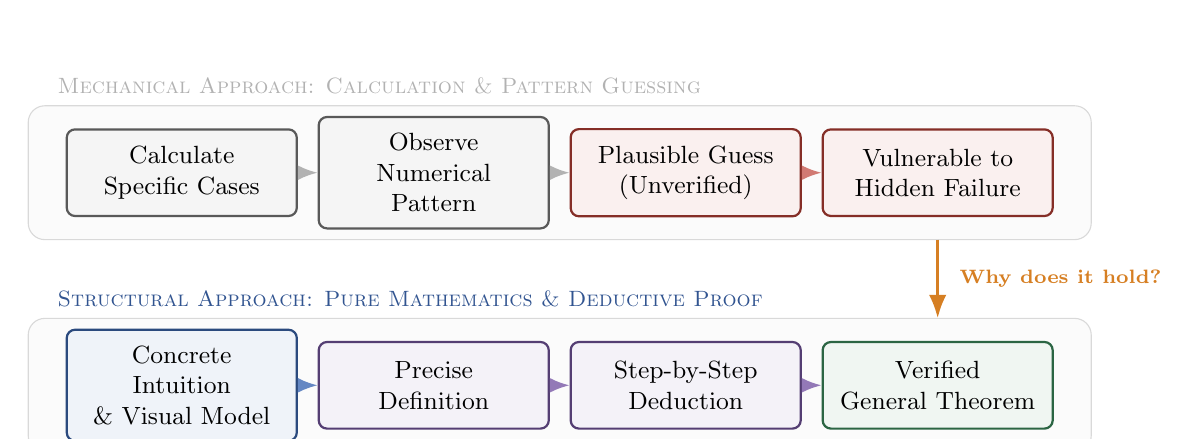
\begin{tikzpicture}[
    node distance=0.8cm,
    font=\small,
    lane/.style={draw=gray!30, fill=gray!3, rounded corners=6pt, inner sep=10pt},
    stepbox/.style={draw=#1!70!black, fill=#1!8, rounded corners=3pt, thick, align=center, inner sep=6pt, text width=2.5cm, minimum height=1.1cm},
    stepbox/.default=sourceblue,
    arrup/.style={-{Latex[length=2.5mm]}, thick, #1},
    arrup/.default=gray!60
]

% Background lanes
\node[lane, minimum width=13.5cm, minimum height=1.7cm] (lane1) at (6.0, 2.3) {};
\node[lane, minimum width=13.5cm, minimum height=1.7cm] (lane2) at (6.0, -0.4) {};

% Labels for lanes
\node[anchor=west, font=\footnotesize\scshape, text=gray!60] at (-0.5, 3.4) {Mechanical Approach: Calculation \& Pattern Guessing};
\node[anchor=west, font=\footnotesize\scshape, text=sourceblue!80!black] at (-0.5, 0.7) {Structural Approach: Pure Mathematics \& Deductive Proof};

% Top lane nodes
\node[stepbox=gray] (c1) at (1.2, 2.3) {Calculate\\Specific Cases};
\node[stepbox=gray] (c2) at (4.4, 2.3) {Observe\\Numerical Pattern};
\node[stepbox=trapred] (c3) at (7.6, 2.3) {Plausible Guess\\(Unverified)};
\node[stepbox=trapred] (c4) at (10.8, 2.3) {Vulnerable to\\Hidden Failure};

\draw[arrup=gray!60] (c1) -- (c2);
\draw[arrup=gray!60] (c2) -- (c3);
\draw[arrup=trapred!70] (c3) -- (c4);

% Transition arrows between lanes
\draw[-{Latex[length=3mm]}, very thick, quotientorange] (10.8, 1.45) -- node[right=4pt, font=\scriptsize\bfseries, text=quotientorange]{Why does it hold?} (10.8, 0.45);

% Bottom lane nodes
\node[stepbox=sourceblue] (p1) at (1.2, -0.4) {Concrete Intuition\\\& Visual Model};
\node[stepbox=structurepurple] (p2) at (4.4, -0.4) {Precise\\Definition};
\node[stepbox=structurepurple] (p3) at (7.6, -0.4) {Step-by-Step\\Deduction};
\node[stepbox=targetgreen] (p4) at (10.8, -0.4) {Verified\\General Theorem};

\draw[arrup=sourceblue!80] (p1) -- (p2);
\draw[arrup=structurepurple!80] (p2) -- (p3);
\draw[arrup=structurepurple!80] (p3) -- (p4);

\end{tikzpicture}
\end{center}

\subsection*{The anatomy of a mathematical concept}

In this text, we resist the urge to hurry into formal proofs before the picture is settled in your mind. Whenever a major concept arrives, you will encounter it through a deliberate sequence:

\begin{itemize}
\item \textbf{The geometric or tactile picture}: What does this look like if you draw it, walk through it, or treat it as a game?
\item \textbf{The minimal formal definition}: What exact requirements are packed into the vocabulary, and why is every single word necessary?
\item \textbf{Examples and deliberate non-examples}: What lives inside the concept, and what sits just outside its boundary?
\item \textbf{Notation decoded}: What is the shorthand saying in plain human terms, and what common reading traps does it set?
\item \textbf{Complete, unhurried proofs}: Every algebraic step and logical pivot explained without hand-waving or skipping the mechanics.
\item \textbf{Walking questions}: Prompts designed to be turned over in your head while away from your desk.
\end{itemize}

\begin{focusbox}
Measure your progress through this book by your ability to work with the concepts independently: after reading an explanation, close the book, take a blank sheet of paper, and verify whether you can state the definitions precisely and explain the reasoning behind the proofs.
\end{focusbox}

\subsection*{The working rule for this text}

When you encounter a new definition, test it immediately against concrete examples. Find a simple object that satisfies it, find a close non-example that fails one condition, and ask what would change if a condition were omitted.

This practice builds immediate familiarity. The theorems in advanced mathematics describe how these definitions interact, so understanding the definitions thoroughly makes following and discovering proofs much more natural.

\begin{recoverybox}
\textbf{Pause and think:} Consider the definition of an \emph{even integer}: an integer $n$ for which there exists an integer $k$ such that $n = 2k$. Test this machine on three edge cases before reading further:
\begin{itemize}
\item Is $0$ even? Check the machine: does an integer $k$ exist with $0 = 2k$? Yes, $k = 0 \in \Z$, so $0$ passes.
\item Is $-6$ even? Check the machine: $-6 = 2(-3)$, and $-3 \in \Z$, so $-6$ passes.
\item Is $2.4$ even? The definition requires $n \in \Z$; $2.4$ is not an integer, so the condition fails immediately.
\end{itemize}
Notice how a formal definition settles questions that everyday intuition might leave uncertain.
\end{recoverybox}

We can visualize a definition as a two-stage filter machine (Figure~\ref{00:fig-definition-machine}).

\begin{figure}[htbp]
\centering
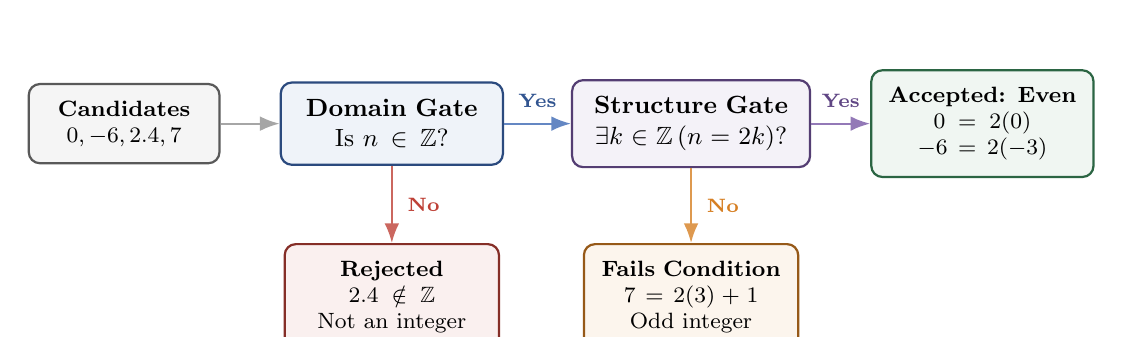
\begin{tikzpicture}[
    font=\small,
    box/.style={draw=#1!70!black, fill=#1!8, rounded corners=4pt, thick, align=center, inner sep=6pt},
    box/.default=sourceblue,
    arrup/.style={-{Latex[length=2.5mm]}, thick, #1},
    arrup/.default=gray!60
]

% Input candidates
\node[box=gray, font=\footnotesize, text width=2.0cm] (in) at (0, 1.5) {\textbf{Candidates}\\$0, -6, 2.4, 7$};

% Gate 1: Domain
\node[box=sourceblue, text width=2.4cm] (g1) at (3.4, 1.5) {\textbf{Domain Gate}\\Is $n \in \Z$?};

% Rejection 1
\node[box=trapred, text width=2.3cm, font=\footnotesize] (r1) at (3.4, -0.7) {\textbf{Rejected}\\$2.4 \notin \Z$\\Not an integer};

% Gate 2: Structure
\node[box=structurepurple, text width=2.6cm] (g2) at (7.2, 1.5) {\textbf{Structure Gate}\\$\exists k \in \Z \, (n = 2k)$?};

% Rejection 2
\node[box=quotientorange, text width=2.3cm, font=\footnotesize] (r2) at (7.2, -0.7) {\textbf{Fails Condition}\\$7 = 2(3) + 1$\\Odd integer};

% Accepted
\node[box=targetgreen, text width=2.4cm, font=\footnotesize] (acc) at (10.9, 1.5) {\textbf{Accepted: Even}\\$0 = 2(0)$\\$-6 = 2(-3)$};

% Arrows
\draw[arrup=gray!70] (in) -- (g1);
\draw[arrup=sourceblue!80] (g1) -- node[above=2pt, font=\scriptsize\bfseries, text=sourceblue!80!black]{Yes} (g2);
\draw[arrup=trapred!80] (g1) -- node[right=2pt, font=\scriptsize\bfseries, text=trapred]{No} (r1);
\draw[arrup=structurepurple!80] (g2) -- node[above=2pt, font=\scriptsize\bfseries, text=structurepurple!80!black]{Yes} (acc);
\draw[arrup=quotientorange!80] (g2) -- node[right=2pt, font=\scriptsize\bfseries, text=quotientorange]{No} (r2);

\end{tikzpicture}
\caption{The definition as an inspection machine. Candidate inputs face sequential gates: first a domain check ($n \in \Z$), then the algebraic condition ($\exists k \in \Z$ with $n = 2k$). Candidates that satisfy both are accepted as even; failing either halts the process.}
\label{00:fig-definition-machine}
\end{figure}

\subsection*{From measurement to deductive proof}

Using empirical rules and arithmetic calculations, Egyptian and Babylonian scribes computed canal volumes, granary capacities, and calendar cycles with notable practical accuracy.

Beginning around the sixth century BCE, Greek mathematicians pursued a different goal: explaining why geometric relationships must hold in general. Consider an isosceles triangle (a triangle with two sides of equal length). A surveyor can measure its base angles with a protractor, verify their equality across many drawings, and observe that the base angles match.

Why, then, did Euclid construct a formal \emph{proof}?

Because a protractor inspects a single physical drawing. It is subject to eyesight and the limits of the instrument. It can confirm that the base angles match within a fraction of a degree, but it cannot establish that the difference is strictly zero. More fundamentally, measuring a thousand triangles cannot guarantee that every possible isosceles triangle shares the same property.

Deductive proof shifts the focus from measurement to structure (Figure~\ref{00:fig-measurement-vs-proof}). Instead of measuring the angles, we draw the vertical axis of symmetry $AD$. By Side-Angle-Side congruence (triangles sharing two sides and the angle between them are identical), the left half $\triangle ABD$ and the right half $\triangle ACD$ are mirror reflections. The equality $\angle B = \angle C$ does not depend on measurement precision; it follows deductively from the symmetry of the figure.

\begin{figure}[htbp]
\centering
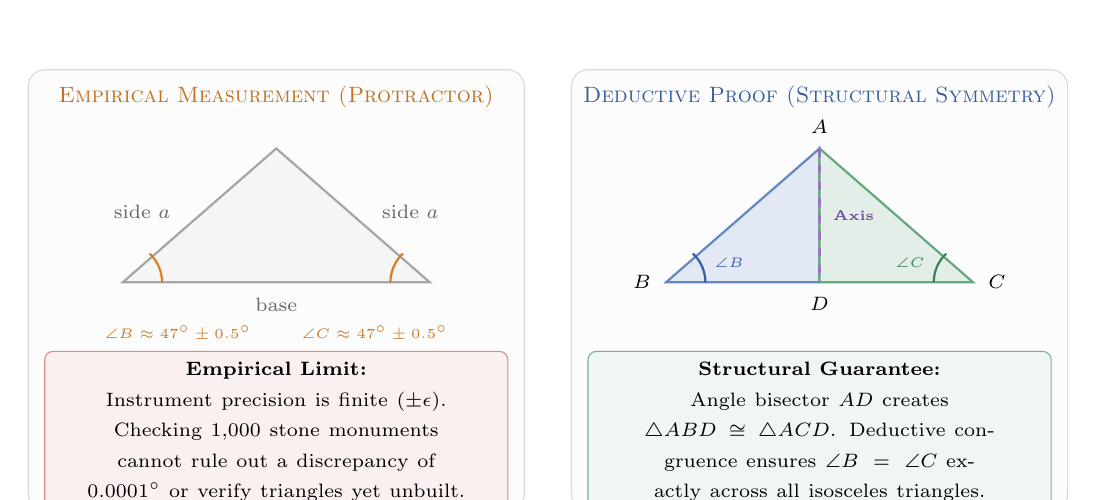
\begin{tikzpicture}[
    font=\small,
    panel/.style={draw=gray!30, fill=gray!2, rounded corners=6pt, inner sep=8pt}
]

% Panel 1: Empirical Measurement
\node[panel, minimum width=6.3cm, minimum height=5.6cm] (p1) at (3.15, 2.0) {};
\node[font=\footnotesize\scshape, text=quotientorange!90!black] at (3.15, 4.45) {Empirical Measurement (Protractor)};

% Triangle in Panel 1
\coordinate (A1) at (3.15, 3.8);
\coordinate (B1) at (1.2, 2.1);
\coordinate (C1) at (5.1, 2.1);

\draw[thick, draw=gray!70, fill=gray!8] (A1) -- (B1) -- (C1) -- cycle;

% Dimension labels
\node[left=2pt, font=\scriptsize, text=gray!80!black] at (2.0, 3.0) {side $a$};
\node[right=2pt, font=\scriptsize, text=gray!80!black] at (4.3, 3.0) {side $a$};
\node[below=2pt, font=\scriptsize, text=gray!80!black] at (3.15, 2.1) {base};

% Angle arcs and callouts
\draw[thick, quotientorange] (1.7, 2.1) arc (0:47:0.5);
\draw[thick, quotientorange] (4.6, 2.1) arc (180:133:0.5);

\node[font=\tiny\bfseries, text=quotientorange!95!black, align=center] at (1.9, 1.45) {$\angle B \approx 47^\circ \pm 0.5^\circ$};
\node[font=\tiny\bfseries, text=quotientorange!95!black, align=center] at (4.4, 1.45) {$\angle C \approx 47^\circ \pm 0.5^\circ$};

\node[draw=trapred!60, fill=trapred!8, rounded corners=3pt, text width=5.6cm, align=center, inner sep=4pt] at (3.15, 0.2) {
    \scriptsize\textbf{Empirical Limit:}\\
    Instrument precision is finite ($\pm \epsilon$). Checking 1,000 stone monuments cannot rule out a discrepancy of $0.0001^\circ$ or verify triangles yet unbuilt.
};

% Panel 2: Deductive Symmetry
\node[panel, minimum width=6.3cm, minimum height=5.6cm] (p2) at (10.05, 2.0) {};
\node[font=\footnotesize\scshape, text=sourceblue!90!black] at (10.05, 4.45) {Deductive Proof (Structural Symmetry)};

% Triangle in Panel 2
\coordinate (A2) at (10.05, 3.8);
\coordinate (B2) at (8.1, 2.1);
\coordinate (C2) at (12.0, 2.1);
\coordinate (D2) at (10.05, 2.1);

% Shaded congruent halves
\draw[fill=sourceblue!15, draw=sourceblue!80, thick] (A2) -- (B2) -- (D2) -- cycle;
\draw[fill=targetgreen!15, draw=targetgreen!80, thick] (A2) -- (D2) -- (C2) -- cycle;

% Symmetry spine
\draw[very thick, dashed, structurepurple!80] (A2) -- (D2) node[midway, right=1pt, font=\tiny\bfseries, text=structurepurple!90!black] {Axis};

% Labels
\node[above=2pt, font=\scriptsize] at (A2) {$A$};
\node[left=2pt, font=\scriptsize] at (B2) {$B$};
\node[right=2pt, font=\scriptsize] at (C2) {$C$};
\node[below=2pt, font=\scriptsize] at (D2) {$D$};

% Angle marks
\draw[thick, sourceblue!90!black] (8.6, 2.1) arc (0:47:0.5);
\node[font=\tiny\bfseries, text=sourceblue!90!black] at (8.9, 2.35) {$\angle B$};

\draw[thick, targetgreen!90!black] (11.5, 2.1) arc (180:133:0.5);
\node[font=\tiny\bfseries, text=targetgreen!90!black] at (11.2, 2.35) {$\angle C$};

% Congruence note
\node[draw=targetgreen!70, fill=targetgreen!8, rounded corners=3pt, text width=5.6cm, align=center, inner sep=4pt] at (10.05, 0.2) {
    \scriptsize\textbf{Structural Guarantee:}\\
    Angle bisector $AD$ creates $\triangle ABD \cong \triangle ACD$. Deductive congruence ensures $\angle B = \angle C$ exactly across all isosceles triangles.
};

\end{tikzpicture}
\caption{Measurement versus proof. \textbf{Left}: A physical protractor inspects a concrete triangle. It confirms equality up to instrument tolerance ($\pm \epsilon$), but cannot guarantee zero discrepancy or speak about triangles not yet measured. \textbf{Right}: A deductive argument constructs the axis of symmetry $AD$. By Side-Angle-Side congruence, the left half is an exact mirror reflection of the right half, establishing that the base angles are equal for every isosceles triangle.}
\label{00:fig-measurement-vs-proof}
\end{figure}

\begin{historybox}
The limits of physical measurement became sharp with the Pythagorean discovery of incommensurability (quantities that share no common measuring unit). The early Pythagoreans believed every geometric relationship was a ratio of whole numbers. When measuring the diagonal of a unit square against its side, they expected a fine enough unit to divide evenly into both. Instead, deductive proof revealed that no such unit exists: the ratio is $\sqrt{2}$, an irrational number (it cannot be written as a fraction of integers $a/b$). Legend says Hippasus of Metapontum was drowned at sea for revealing this result. Physical measurement produces approximations like $1.414$ or $1.41421356$, but only deductive proof could show that the ratio is not a fraction.

Euclid's breakthrough in the \emph{Elements} (c.~300 BCE) was to replace physical measurement with an axiomatic framework. Starting from minimal definitions and five geometric postulates (such as ``a straight line can be drawn between any two points''), each proposition was deduced step by step.

Even so, Euclid's system left gaps. His synthetic geometry (geometry built directly from axioms without coordinates) relied implicitly on diagrams---for instance, assuming without proof that two circles must intersect if their centers are close enough. In 1899, David Hilbert supplied a complete set of axioms. In the nineteenth century, mathematicians also discovered that Euclid's Fifth Postulate (the parallel postulate) can be altered, yielding consistent non-Euclidean geometries. In 1931, Kurt G\"odel showed that no single axiomatic system can be both consistent and complete enough to prove all truths of arithmetic. The search for secure foundations remains an active part of mathematical thinking.
\end{historybox}

The proof that the diagonal of a unit square cannot be expressed as a ratio of whole numbers illustrates the difference between physical approximation and deduction (Figure~\ref{00:fig-incommensurability-diagonal}).

\begin{figure}[htbp]
\centering
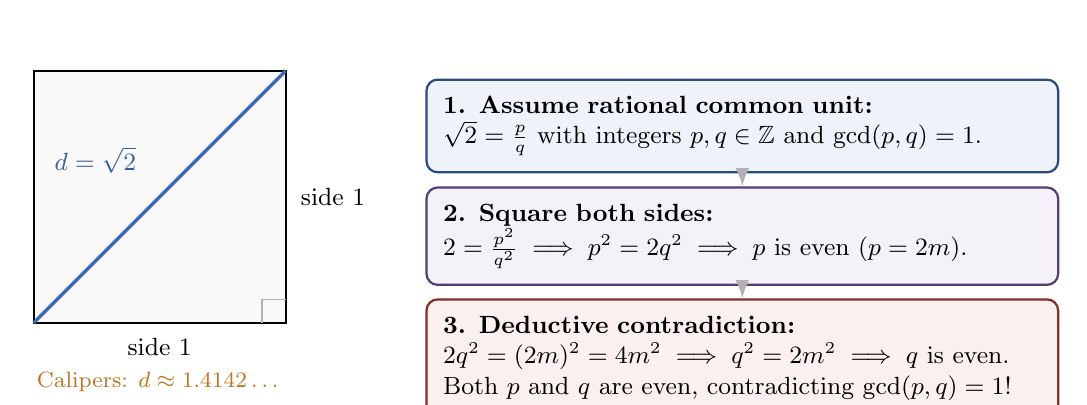
\begin{tikzpicture}[
    font=\small,
    box/.style={draw=#1!70!black, fill=#1!8, rounded corners=4pt, thick, align=left, inner sep=6pt},
    box/.default=sourceblue
]

% Left: The unit square
\draw[thick, fill=gray!5] (0, 0) rectangle (3.2, 3.2);
\draw[very thick, sourceblue] (0, 0) -- (3.2, 3.2);

% Right angle mark at (3.2, 0)
\draw[gray!60] (2.9, 0) -- (2.9, 0.3) -- (3.2, 0.3);

% Labels on the square
\node[below=2pt, font=\small] at (1.6, 0) {side $1$};
\node[right=2pt, font=\small] at (3.2, 1.6) {side $1$};
\node[above left=-1pt, font=\small\bfseries, text=sourceblue!90!black] at (1.4, 1.8) {$d = \sqrt{2}$};

% Caliper approximation callout below
\node[font=\footnotesize, text=quotientorange!90!black, align=center] at (1.6, -0.75) {Calipers: $d \approx 1.4142\dots$};

% Right: Contradiction steps
\node[box=sourceblue, text width=7.6cm] (step1) at (9.0, 2.5) {
    \textbf{1. Assume rational common unit:}\\
    $\sqrt{2} = \frac{p}{q}$ with integers $p, q \in \Z$ and $\gcd(p,q) = 1$.
};

\node[box=structurepurple, text width=7.6cm] (step2) at (9.0, 1.1) {
    \textbf{2. Square both sides:}\\
    $2 = \frac{p^2}{q^2} \implies p^2 = 2q^2 \implies p$ is even ($p = 2m$).
};

\node[box=trapred, text width=7.6cm] (step3) at (9.0, -0.45) {
    \textbf{3. Deductive contradiction:}\\
    $2q^2 = (2m)^2 = 4m^2 \implies q^2 = 2m^2 \implies q$ is even.\\
    Both $p$ and $q$ are even, contradicting $\gcd(p,q) = 1$!
};

\draw[-{Latex}, thick, gray!60] (step1) -- (step2);
\draw[-{Latex}, thick, gray!60] (step2) -- (step3);

\end{tikzpicture}
\caption{Incommensurability of the diagonal. Physical calipers can only approximate $d \approx 1.4142$, never ruling out a rational fraction with a large denominator. Deductive proof establishes that assuming $\sqrt{2} = p/q$ forces both $p$ and $q$ to be even, an impossible contradiction that proves no such fraction exists.}
\label{00:fig-incommensurability-diagonal}
\end{figure}

\subsection*{What beginner-friendly means here}

Being accessible does not mean avoiding technical precision; it means ensuring every logical step is clearly explained. We introduce concepts with concrete motivation and visual intuition, but every explanation leads directly to precise definitions and verifiable deductions. The goal is to make rigorous mathematical reasoning understandable from the ground up.

In Chapter~1 (\emph{The Change in Game: From Getting Answers to Giving Reasons}), we make this transition concrete. We will examine a formula that holds for billions of consecutive numbers before abruptly failing, and see why numerical calculation cannot substitute for deductive proof.

\subsection*{Exercises}

\begin{enumerate}
\item \textbf{Laser measurement versus deductive proof.} Suppose you build a physical triangle out of machined steel rods whose lengths agree to within one micrometer ($10^{-6}\text{ m}$). A laser sensor measures the three angles and reports $59.999^\circ$, $60.001^\circ$, and $60.000^\circ$. Have you proven that an equilateral triangle has equal angles? What does a deductive proof provide that the physical sensor can never deliver?

\item \textbf{The machine test: why $1$ is not prime.} A student argues: ``Since $1$ is only divisible by $1$ and itself, $1$ must be a prime number.'' Mathematicians define a prime number as an integer $p > 1$ whose only positive divisors are $1$ and $p$. Why is the requirement $p > 1$ deliberately included in the definition machine? (Hint: Consider what happens to the Fundamental Theorem of Arithmetic---which states that every integer greater than $1$ factors into prime numbers in exactly one way---if $1$ were counted as a prime.)

\item \textbf{Boundary testing on a definition machine.} Consider the definition: ``An integer $n$ is \emph{composite} if there exist integers $a > 1$ and $b > 1$ such that $n = ab$.'' Test each candidate number against this machine and state whether it is accepted, rejected, or outside the domain of definition:
\begin{enumerate}[label=(\alph*)]
\item $n = 12$
\item $n = 7$
\item $n = 1$
\item $n = 0$
\item $n = -6$
\end{enumerate}

\item \textbf{Testing claims on numbers.} Consider the claim: ``For every real number $x$, if $x > 0$, then $x^2 > x$.''
\begin{enumerate}[label=(\alph*)]
\item Find two numbers that easily satisfy this claim.
\item Test the boundary value $x = 1$. Does $1^2 > 1$?
\item Test the value $x = 1/2$. Does $(1/2)^2 > 1/2$?
\item Describe the exact collection of positive real numbers for which the claim $x^2 > x$ is actually true.
\end{enumerate}

\item \textbf{Incommensurability and proof.} In your own words, explain why the discovery that the diagonal of a unit square cannot be written as a fraction of integers ($a/b$) could never have been made using bronze calipers or numerical tables alone. What role did deductive contradiction play in uncovering this fact?
\end{enumerate}

\begin{walkbox}
Consider a mathematical formula you frequently use, such as the quadratic formula or the Pythagorean theorem. Can you derive it from first principles, or do you rely on it as a memorized procedure? What definitions and intermediate steps are required to turn that formula into a complete deductive proof?
\end{walkbox}

\newpage

\section{The Change in Game: From Getting Answers to Giving Reasons}
\chapterline

In the opening pages of this book (\emph{How This Book Should Be Read}), we distinguished between calculating numerical answers and providing deductive proofs. If your background is in engineering or applied science, your training naturally directs your attention toward methods of solution. When you encounter a system of linear equations, you reach for Gaussian elimination or matrix factorizations. When a differential equation appears, you check whether it is separable, linear, or amenable to an integrating factor. When an integral looks intimidating, you scan your mental catalog for substitutions, integration by parts, or numerical quadrature.

That computational agility is valuable. But pure mathematics asks you to pause before reaching for an algorithm. It shifts the central question from \emph{what is the answer?} to something fundamentally different:

\begin{quote}
\itshape What exact claim is being made here, and why is it logically impossible for it to fail under our assumptions?
\end{quote}

Answering that question requires a different kind of argument than computing a result.

\subsection{Checking numbers versus establishing truth}

Consider a simple numerical experiment. You add consecutive odd numbers and watch the running totals emerge:
\begin{align*}
1 &= 1 = 1^2, \\
1 + 3 &= 4 = 2^2, \\
1 + 3 + 5 &= 9 = 3^2, \\
1 + 3 + 5 + 7 &= 16 = 4^2, \\
1 + 3 + 5 + 7 + 9 &= 25 = 5^2.
\end{align*}

A striking regularity appears immediately. It is natural to form a conjecture---a proposed statement believed to be true based on patterns, but not yet proved---that for any positive integer $n$ (where $\N = \{1, 2, 3, \ldots\}$ denotes the natural numbers):
\[
1 + 3 + 5 + \cdots + (2n - 1) = n^2.
\]

You could write a quick script to test this equation for $n = 10$, $n = 1{,}000$, or even the first ten billion natural numbers. Every single test will return a match. 

In engineering, ten billion consecutive successful trials is strong empirical evidence. In pure mathematics, however, those ten billion checks leave infinitely many natural numbers untested. Checking specific numbers, no matter how many, cannot prove a claim for every natural number $n$.

This exact dilemma confronted Thales, Pythagoras, and Euclid in the sixth through third centuries BCE. Working with sand trays, straightedges, and counting pebbles, the early Greeks realized that empirical testing is inherently limited on infinite sets.

Several famous conjectures held for thousands or millions of test cases before failing at a single counterexample---a concrete instance where a general claim fails:
\begin{itemize}
\item \textbf{Fermat's Prime Conjecture (1640)}: Pierre de Fermat noticed that the numbers $F_n = 2^{2^n} + 1$ are prime (whole numbers greater than $1$ with no positive divisors other than $1$ and themselves) for $n = 0, 1, 2, 3, 4$:
\[
F_0 = 3, \quad F_1 = 5, \quad F_2 = 17, \quad F_3 = 257, \quad F_4 = 65{,}537.
\]
All five are prime. Fermat conjectured that $F_n$ is prime for \emph{every} natural number $n$. Almost a century later, in 1732, Leonhard Euler factored the very next case:
\[
F_5 = 2^{32} + 1 = 4{,}294{,}967{,}297 = 641 \times 6{,}700{,}417.
\]
In fact, no other Fermat prime has ever been discovered.
\item \textbf{Euler's Sum of Powers (1769)}: Euler conjectured that at least $k$ positive $k$-th powers are required to sum to another $k$-th power. For fourth powers, this asserted that $a^4 + b^4 + c^4 = d^4$ has no positive integer solutions. For more than two centuries, mathematicians found no counterexample, and twentieth-century computer searches turned up nothing. Yet in 1986, using elliptic curves and algebraic geometry, Noam Elkies showed that a counterexample exists:
\[
2{,}682{,}440^4 + 15{,}365{,}639^4 + 18{,}796{,}760^4 = 20{,}615{,}673^4.
\]
\item \textbf{The P\'olya Conjecture (1919)}: George P\'olya conjectured that for any integer $n > 1$, at least half of the integers up to $n$ have an odd number of prime factors (counted with repetition, so $12 = 2 \times 2 \times 3$ has three prime factors, which is odd, while $4 = 2 \times 2$ has two, which is even). The conjecture was verified for millions of integers. It holds without exception for every single number up to $906{,}150{,}256$. The smallest counterexample only appears at $n = 906{,}150{,}257$!
\end{itemize}

If mathematicians had stopped checking at nine hundred million, they would have accepted a false claim. Checking individual numbers only verifies finitely many cases; a proof shows why a general statement holds for every $n$.

\begin{recoverybox}
\textbf{Pause and think:} Suppose someone writes a script that tests an arithmetic identity for the first trillion positive integers, and every single case succeeds. In software testing or material science, this is overwhelming evidence. Why does a pure mathematician still refuse to declare the identity true?
\end{recoverybox}

\begin{center}
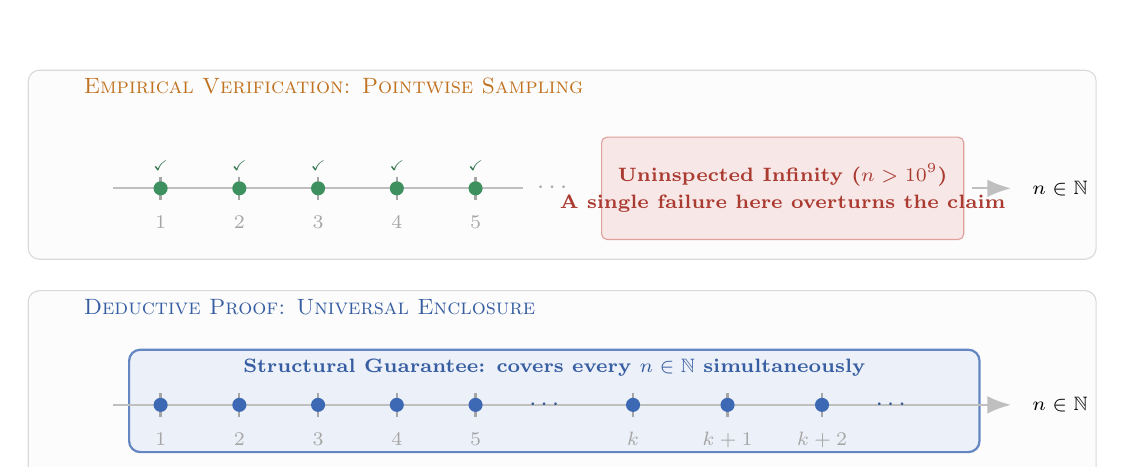
\begin{tikzpicture}[
    font=\small,
    ruler/.style={draw=gray!50, thick},
    panel/.style={draw=gray!30, fill=gray!2, rounded corners=4pt, inner sep=8pt}
]

% Panel A: Sampling
\node[panel, text width=13.0cm, minimum height=2.4cm] (pA) at (6.5, 3.0) {};
\node[anchor=west, font=\footnotesize\scshape, text=quotientorange!90!black] at (0.3, 4.0) {Empirical Verification: Pointwise Sampling};

% Number line for Panel A
\draw[ruler] (0.8, 2.7) -- (6.0, 2.7);
\node[font=\small, text=gray!70] at (6.4, 2.7) {$\cdots$};
\draw[ruler, -{Latex[length=3mm]}] (11.7, 2.7) -- (12.2, 2.7) node[right=4pt, font=\scriptsize] {$n \in \N$};
\foreach \x/\label in {1.4/1, 2.4/2, 3.4/3, 4.4/4, 5.4/5} {
    \draw[thick, gray!70] (\x, 2.85) -- (\x, 2.55) node[below=2pt, font=\scriptsize] {$\label$};
    \node[circle, fill=targetgreen, inner sep=1.8pt] at (\x, 2.7) {};
    \node[above=3pt, font=\tiny\bfseries, text=targetgreen!80!black] at (\x, 2.7) {\checkmark};
}

% Region of untested numbers
\draw[fill=trapred!12, draw=trapred!50, rounded corners=2pt] (7.0, 2.05) rectangle (11.6, 3.35);
\node[text=trapred!90!black, font=\scriptsize\bfseries, align=center] at (9.3, 2.7) {Uninspected Infinity ($n > 10^9$)\\[2pt]\scriptsize A single failure here overturns the claim};

% Panel B: Deductive Proof
\node[panel, text width=13.0cm, minimum height=2.4cm] (pB) at (6.5, 0.2) {};
\node[anchor=west, font=\footnotesize\scshape, text=sourceblue!90!black] at (0.3, 1.2) {Deductive Proof: Universal Enclosure};

% Enclosure boundary
\draw[draw=sourceblue!80, fill=sourceblue!10, rounded corners=4pt, thick] (1.0, -0.65) rectangle (11.8, 0.65);
\node[text=sourceblue!90!black, font=\scriptsize\bfseries, align=center] at (6.4, 0.42) {Structural Guarantee: covers every $n \in \N$ simultaneously};

\draw[ruler, -{Latex[length=3mm]}] (0.8, -0.05) -- (12.2, -0.05) node[right=4pt, font=\scriptsize] {$n \in \N$};
\foreach \x/\label in {1.4/1, 2.4/2, 3.4/3, 4.4/4, 5.4/5} {
    \draw[thick, gray!70] (\x, 0.10) -- (\x, -0.20) node[below=2pt, font=\scriptsize] {$\label$};
    \node[circle, fill=sourceblue, inner sep=1.8pt] at (\x, -0.05) {};
}
\node[font=\small, text=sourceblue!80!black] at (6.3, -0.05) {$\cdots$};
\foreach \x/\label in {7.4/k, 8.6/k+1, 9.8/k+2} {
    \draw[thick, gray!70] (\x, 0.10) -- (\x, -0.20) node[below=2pt, font=\scriptsize] {$\label$};
    \node[circle, fill=sourceblue, inner sep=1.8pt] at (\x, -0.05) {};
}
\node[font=\small, text=sourceblue!80!black] at (10.7, -0.05) {$\cdots$};

\end{tikzpicture}\\[0.4em]
{\small\textbf{Figure 1.1:} \textit{Pointwise sampling versus universal enclosure.} Empirical verification (top) tests individual numbers, leaving infinitely many uninspected values where a counterexample can hide. Deductive proof (bottom) identifies an underlying structural relationship that establishes all infinitely many cases at once.}
\end{center}

To establish that our odd-number pattern holds across the entire infinite tail in Figure~1.1, we need a single structural argument that covers every $n$ at once.

\subsection{Seeing the reason geometrically}

Why \emph{must} the sum of the first $n$ odd numbers equal $n^2$? We do not need a computer to check cases. We can arrange the numbers visually into a square.

Start with a single $1 \times 1$ block. To expand this block into a $2 \times 2$ square, you must wrap around its top and right edges. How many new unit squares are required? Exactly $3$. 

To expand the $2 \times 2$ square into a $3 \times 3$ square, you again wrap an L-shaped band around the outer border. That band consists of two sides of length $2$, plus the single corner block where they meet: $2 + 2 + 1 = 5$ unit squares.

\begin{center}
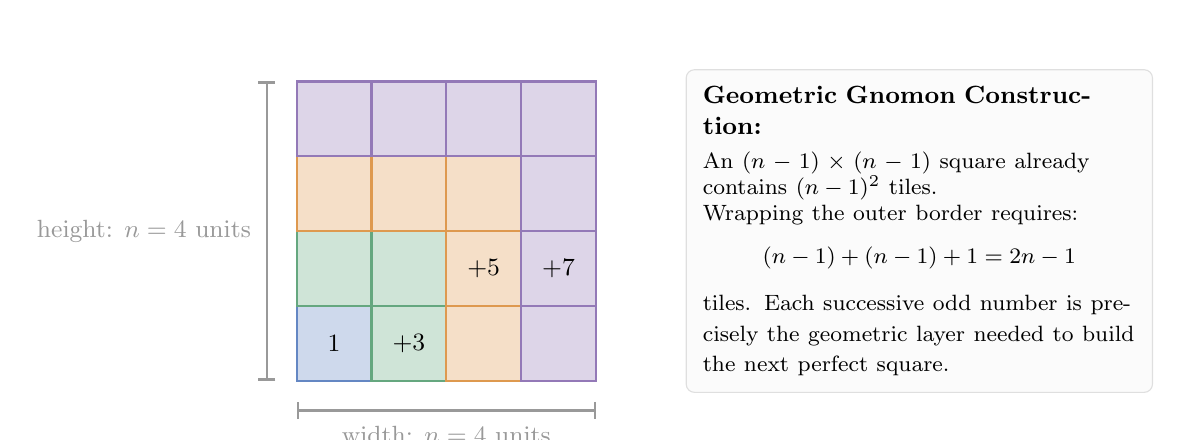
\begin{tikzpicture}[scale=0.95, font=\small]

% 1x1 block
\draw[fill=sourceblue!25, draw=sourceblue!80, thick] (0,0) rectangle (1,1);
\node at (0.5, 0.5) {$1$};

% 2x2 layer (3 blocks)
\draw[fill=targetgreen!25, draw=targetgreen!80, thick] (1,0) rectangle (2,1);
\draw[fill=targetgreen!25, draw=targetgreen!80, thick] (1,1) rectangle (2,2);
\draw[fill=targetgreen!25, draw=targetgreen!80, thick] (0,1) rectangle (1,2);
\node at (1.5, 0.5) {$+3$};
\node at (1.5, 1.5) {};
\node at (0.5, 1.5) {};

% 3x3 layer (5 blocks)
\foreach \x/\y in {2/0, 2/1, 2/2, 1/2, 0/2} {
    \draw[fill=quotientorange!25, draw=quotientorange!80, thick] (\x,\y) rectangle (\x+1,\y+1);
}
\node at (2.5, 1.5) {$+5$};

% 4x4 layer (7 blocks)
\foreach \x/\y in {3/0, 3/1, 3/2, 3/3, 2/3, 1/3, 0/3} {
    \draw[fill=structurepurple!25, draw=structurepurple!80, thick] (\x,\y) rectangle (\x+1,\y+1);
}
\node at (3.5, 1.5) {$+7$};

% Dimension annotations
\draw[|-|, thick, gray!80] (0, -0.4) -- (4, -0.4) node[midway, below=2pt] {width: $n = 4$ units};
\draw[|-|, thick, gray!80] (-0.4, 0) -- (-0.4, 4) node[midway, left=2pt] {height: $n = 4$ units};

% Legend / Explanation on the right
\node[anchor=west, text width=5.5cm, inner sep=6pt, fill=gray!3, draw=gray!25, rounded corners=3pt] at (5.2, 2.0) {
    \textbf{Geometric Gnomon Construction:}\\[0.3em]
    \footnotesize
    An $(n-1) \times (n-1)$ square already contains $(n-1)^2$ tiles.\\
    Wrapping the outer border requires:
    \[
    (n-1) + (n-1) + 1 = 2n - 1
    \]
    tiles. Each successive odd number is precisely the geometric layer needed to build the next perfect square.
};

\end{tikzpicture}\\[0.4em]
{\small\textbf{Figure 1.2:} \textit{The geometric gnomon construction.} Successive odd numbers wrap around an existing square like nested shells. Expanding an $(n-1) \times (n-1)$ square to an $n \times n$ square requires two strips of length $n-1$ plus a single corner tile: $(n-1) + (n-1) + 1 = 2n-1$ tiles. The algebraic expansion and the geometric tiling match exactly.}
\end{center}

In general, if you already have an $(n-1) \times (n-1)$ square containing $(n-1)^2$ tiles, completing the $n \times n$ square requires adding:
\[
n^2 - (n-1)^2 = n^2 - (n^2 - 2n + 1) = 2n - 1
\]
new tiles. Geometrically, this breaks into two arms of length $n-1$ along the top and right, plus $1$ single corner block where they meet:
\[
(n - 1) + (n - 1) + 1 = 2n - 1.
\]
This L-shaped border (known since ancient Greek geometry as a \emph{gnomon}, from the Greek word for a carpenter's square or indicator) shows that the $n$-th odd number is structurally tailored to convert an $(n-1)^2$ square into an $n^2$ square. 

We did not need to test individual cases up to $n = 10^{12}$. The geometric argument reveals the algebraic reason that forces the equation to hold across all natural numbers at once.

\begin{recoverybox}
\textbf{Pause and think:} Look at the gnomon equation $n^2 - (n-1)^2 = 2n - 1$. What happens if you add consecutive \emph{even} numbers instead: $2 + 4 + 6 + \cdots + 2n$? Can you picture what shape is formed if you attach one extra column of unit tiles to the side of the square? (Can you see why the sum is $n(n+1)$?)
\end{recoverybox}

\subsection{From formulas to structural invariants}

In engineering, formulas often serve as compact input-output converters:
\[
\vec{F} = m\vec{a}, \qquad e^{i\theta} = \cos\theta + i\sin\theta, \qquad A\vec{x} = \vec{b}.
\]
In pure mathematics, formulas are often consequences of broader geometric and algebraic structures. Instead of asking only what numerical output a formula produces, pure mathematics investigates the structural rules governing the systems where the formula lives:
\begin{itemize}
\item What is a \emph{set} (a well-defined collection of distinct objects), and how do we build collections without falling into self-referential paradoxes?
\item What is a \emph{function} (not merely an algebraic formula like $f(x) = x^2$, but an unambiguous assignment from each element of an input domain to an output target)?
\item What does it mean for two mathematical systems to share the ``same structure''---an \emph{isomorphism} (from the Greek \emph{isos} ``equal'' and \emph{morphe} ``form'': a structural dictionary that matches every element and operation of one system to another without loss of information)?
\item What properties remain \emph{invariant} (unchanged under transformations, such as stretching, twisting, or coordinate shifts)?
\end{itemize}

This shift toward abstraction unifies seemingly unrelated problems. A single theorem about \emph{groups}---mathematical systems capturing symmetry, defined as collections of actions that can be combined and undone under strict rules---explains properties of modular arithmetic, geometric symmetries of crystals, roots of polynomial equations, and conservation laws in physics.

\begin{historybox}
Early Greek mathematicians studied number theory by arranging pebbles (\emph{psephoi}, from which the word \emph{calculus} originates) into geometric arrays: triangles, squares, and rectangles. The L-shaped gnomon was not an abstract algebraic trick; it was a physical wooden carpenter's square placed around an existing pebble array to enlarge it.

The limitation of pebble arithmetic and empirical testing is that physical arrangements only verify finitely many instances at a time. The shift to deductive proof---exemplified by Euclid's \emph{Elements}---aimed to capture all infinitely many cases at once by analyzing the structure rather than counting stones.
\end{historybox}

\subsection{General proofs and the limits of visual intuition}

A structural argument like our gnomon tiling covers every positive integer $n$ at once, rather than checking values one by one.

Even so, visual and geometric reasoning has a real limitation: \textbf{our eyes can easily be deceived}. Drawings rely on physical ink and human visual perception, both of which have finite resolution. A slight tilt or a tiny gap can easily pass unnoticed, making false arguments appear plausible.

To see how unassisted visual intuition can be misleading, consider the classic dissection paradox shown in Figure~1.3. An $8 \times 8$ square of area $64$ is sliced into four pieces: two right triangles (each with legs $3$ and $8$, area $12$) and two trapezoids (each with parallel sides $3$ and $5$ and width $5$, area $20$). When rearranged, the pieces appear to fit together into a $13 \times 5$ rectangle of area $65$.

\begin{center}
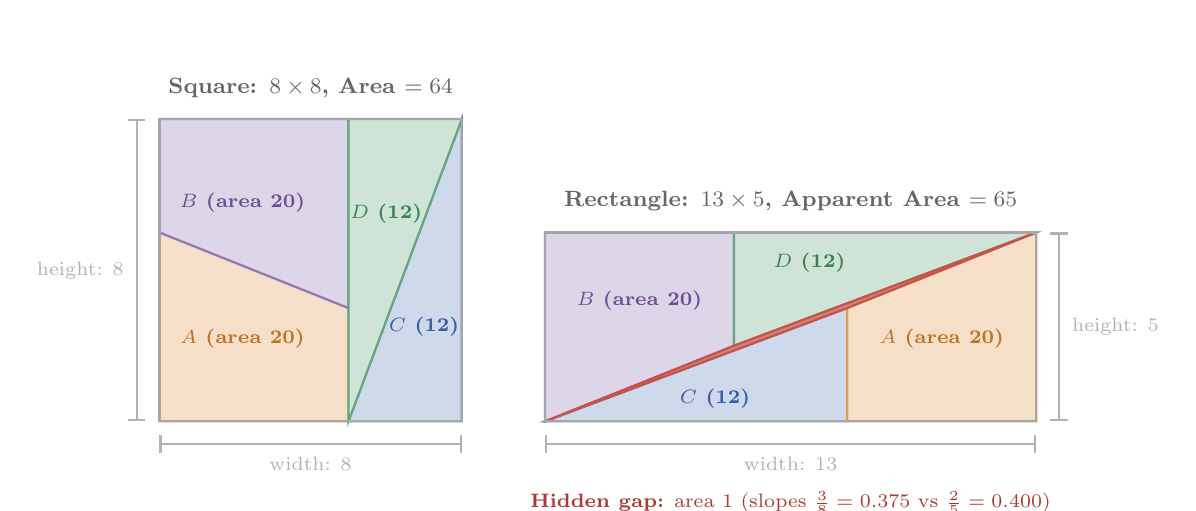
\begin{tikzpicture}[scale=0.48, font=\small]

% Panel 1: The 8x8 Square (Area 64)
\begin{scope}[xshift=0cm]
    \node[anchor=south, font=\footnotesize\bfseries\scshape, text=gray!80!black] at (4, 8.3) {Square: $8 \times 8$, Area $= 64$};
    
    % Grid
    \draw[step=1, gray!18, very thin] (0,0) grid (8,8);
    
    % Trapezoid A (lower-left)
    \filldraw[fill=quotientorange!25, draw=quotientorange!80, thick] (0,0) -- (5,0) -- (5,3) -- (0,5) -- cycle;
    \node[text=quotientorange!90!black, font=\scriptsize\bfseries] at (2.2, 2.2) {$A$ (area 20)};
    
    % Trapezoid B (upper-left)
    \filldraw[fill=structurepurple!25, draw=structurepurple!80, thick] (0,5) -- (5,3) -- (5,8) -- (0,8) -- cycle;
    \node[text=structurepurple!90!black, font=\scriptsize\bfseries] at (2.2, 5.8) {$B$ (area 20)};
    
    % Triangle C (lower-right)
    \filldraw[fill=sourceblue!25, draw=sourceblue!80, thick] (5,0) -- (8,0) -- (8,8) -- cycle;
    \node[text=sourceblue!90!black, font=\scriptsize\bfseries] at (7.0, 2.5) {$C$ (12)};
    
    % Triangle D (upper-right)
    \filldraw[fill=targetgreen!25, draw=targetgreen!80, thick] (5,0) -- (5,8) -- (8,8) -- cycle;
    \node[text=targetgreen!90!black, font=\scriptsize\bfseries] at (6.0, 5.5) {$D$ (12)};
    
    % Outer border
    \draw[thick, gray!70] (0,0) rectangle (8,8);
    \draw[|-|, thick, gray!60] (0, -0.6) -- (8, -0.6) node[midway, below=1pt, font=\scriptsize] {width: $8$};
    \draw[|-|, thick, gray!60] (-0.6, 0) -- (-0.6, 8) node[midway, left=1pt, font=\scriptsize] {height: $8$};
\end{scope}

% Panel 2: The 13x5 Rectangle (Apparent Area 65)
\begin{scope}[xshift=10.2cm, yshift=0cm]
    \node[anchor=south, font=\footnotesize\bfseries\scshape, text=gray!80!black] at (6.5, 5.3) {Rectangle: $13 \times 5$, Apparent Area $= 65$};
    
    % Grid
    \draw[step=1, gray!18, very thin] (0,0) grid (13,5);
    
    % Triangle C (bottom-left)
    \filldraw[fill=sourceblue!25, draw=sourceblue!80, thick] (0,0) -- (8,0) -- (8,3) -- cycle;
    \node[text=sourceblue!90!black, font=\scriptsize\bfseries] at (4.5, 0.6) {$C$ (12)};
    
    % Trapezoid A (bottom-right)
    \filldraw[fill=quotientorange!25, draw=quotientorange!80, thick] (8,0) -- (13,0) -- (13,5) -- (8,3) -- cycle;
    \node[text=quotientorange!90!black, font=\scriptsize\bfseries] at (10.5, 2.2) {$A$ (area 20)};
    
    % Trapezoid B (top-left)
    \filldraw[fill=structurepurple!25, draw=structurepurple!80, thick] (0,0) -- (5,2) -- (5,5) -- (0,5) -- cycle;
    \node[text=structurepurple!90!black, font=\scriptsize\bfseries] at (2.5, 3.2) {$B$ (area 20)};
    
    % Triangle D (top-right)
    \filldraw[fill=targetgreen!25, draw=targetgreen!80, thick] (5,2) -- (13,5) -- (5,5) -- cycle;
    \node[text=targetgreen!90!black, font=\scriptsize\bfseries] at (7.0, 4.2) {$D$ (12)};
    
    % Parallelogram gap (vertices (0,0), (5,2), (13,5), (8,3))
    \filldraw[fill=trapred!65, draw=trapred!90, thick] (0,0) -- (5,2) -- (13,5) -- (8,3) -- cycle;
    
    % Outer border
    \draw[thick, gray!70] (0,0) rectangle (13,5);
    \draw[|-|, thick, gray!60] (0, -0.6) -- (13, -0.6) node[midway, below=1pt, font=\scriptsize] {width: $13$};
    \draw[|-|, thick, gray!60] (13.6, 0) -- (13.6, 5) node[midway, right=1pt, font=\scriptsize] {height: $5$};
    
    % Note on gap
    \node[anchor=north, font=\scriptsize, text=trapred!90!black] at (6.5, -1.6) {\textbf{Hidden gap:} area $1$ (slopes $\frac{3}{8} = 0.375$ vs $\frac{2}{5} = 0.400$)};
\end{scope}

\end{tikzpicture}\\[0.4em]
{\small\textbf{Figure 1.3:} \textit{The chessboard dissection paradox ($64 \ne 65$).} Slicing an $8 \times 8$ square (left) yields four pieces totaling area $64$. Reassembling them into a $13 \times 5$ rectangle (right) seems to produce area $65$. The illusion arises because the human eye cannot see the slight bend along the diagonal: the triangle's slope is $\frac{3}{8} = 0.375$, while the trapezoid's slope is $\frac{2}{5} = 0.400$. The pieces do not meet; they enclose a thin parallelogram gap of area $1$.}
\end{center}

Where did the extra square unit come from?

The human eye sees a clean diagonal line running from $(0,0)$ to $(13,5)$. But calculate the slopes of the abutting pieces:
\[
\text{slope of triangle hypotenuse} = \frac{3}{8} = 0.375, \qquad \text{slope of trapezoid edge} = \frac{2}{5} = 0.400.
\]
Because $\frac{3}{8} \ne \frac{2}{5}$, the pieces do not meet along a straight line. They bend slightly outward, leaving a long, paper-thin parallelogram gap running along the seam. The area of that hidden gap is precisely $1$ unit square:
\[
|5 \times 3 - 8 \times 2| = |15 - 16| = 1.
\]
Because the slope difference is only $0.025$, our visual system smooths over the gap and perceives a solid rectangle. If we relied on pictures alone as proofs, we would be forced to conclude that $64 = 65$.

Geometric drawings also cannot directly represent higher dimensions. We cannot sketch a ten-dimensional vector space or an infinite-dimensional space of continuous functions on a chalkboard.

When visual intuition reaches its practical boundary, mathematics turns to precise symbolic language. In Chapter~2 (\emph{Mathematical Sentences: Statements, Predicates, and Claims}), we begin building that grammar from the ground up, learning how to distinguish expressions from assertions, open conditions from true-or-false statements, and valid deductive arguments from empirical patterns.

\subsection{Exercises: cultivating three perspectives}

\begin{enumerate}[label=\textbf{\arabic*.}]
\item \textbf{Mental Check: Patterns versus Invariants.}
\begin{enumerate}[label=(\alph*)]
\item Consider the polynomial $P(n) = n^2 - n + 41$. Compute $P(1), P(2), P(3), P(4)$. Are all four values prime? (In fact, $P(n)$ produces prime numbers for every integer from $n = 1$ up to $n = 40$.) What happens at $n = 41$? Why does this reinforce the lesson of Figure~1.1?
\item Someone claims that $(n-1)(n-2)(n-3) = 0$ is a universal law for all natural numbers, citing $n = 1, 2, 3$ as evidence. At what value of $n$ does this claim break, and what went wrong with the tester's reasoning?
\end{enumerate}

\item \textbf{Core Practice: Three Perspectives on Odd Numbers.}
For the identity $1 + 3 + 5 + \cdots + (2n-1) = n^2$, write down three distinct explanations:
\begin{enumerate}[label=(\alph*)]
\item A concrete numerical verification for $n = 6$.
\item A paragraph in plain English explaining the geometric gnomon diagram (Figure~1.2) to someone who has never studied algebra.
\item An inductive step: assuming the identity holds for some positive integer $k$, so that $1 + 3 + \cdots + (2k-1) = k^2$, show algebraically how adding the next odd number, $2(k+1) - 1$, produces $(k+1)^2$.
\end{enumerate}

\item \textbf{Core Practice: Summing Consecutive Even Numbers.}
Consider the sum of the first $n$ consecutive even numbers: $2 + 4 + 6 + \cdots + 2n$.
\begin{enumerate}[label=(\alph*)]
\item Calculate the sum for $n = 1, 2, 3, 4$. What pattern emerges in relation to $n(n+1)$?
\item By pairing each odd number in $1 + 3 + 5 + \cdots + (2n-1)$ with $1$ extra unit, deduce geometrically why the even sum forms an $n \times (n+1)$ rectangle of area $n(n+1)$.
\end{enumerate}

\item \textbf{Deeper Reflection: The Anatomy of a Visual Illusion.}
In the chessboard dissection paradox (Figure~1.3), the dimensions $3, 5, 8, 13$ are consecutive terms of the Fibonacci sequence ($F_4 = 3, F_5 = 5, F_6 = 8, F_7 = 13$).
\begin{enumerate}[label=(\alph*)]
\item Calculate Cassini's identity for these indices: $F_5 \times F_7 - F_6^2 = 5 \times 13 - 8^2$.
\item What happens to the slopes $\frac{F_{k-1}}{F_{k+1}}$ and $\frac{F_{k-2}}{F_k}$ as the Fibonacci indices grow larger? Does the gap become easier or harder for the human eye to detect?
\end{enumerate}
\end{enumerate}

\begin{walkbox}
Take an equation or rule of thumb you rely on frequently in your own work. Do you know the precise boundary conditions where it ceases to be true? What hidden assumption prevents it from failing?
\end{walkbox}

\newpage

\section{Mathematical Sentences: Statements, Predicates, and Claims}
\chapterline

Before constructing proofs, we need to inspect the grammar of mathematical language. This is not grammar in the sense of memorizing punctuation rules. It is the physics of how symbols fit together: what kinds of objects exist, which expressions refer to things, which expressions make claims, and which claims can be evaluated as true or false.

\begin{historybox}
For more than two thousand years, formal logic was synonymous with Aristotle's syllogisms (c.~350 BCE in the \emph{Prior Analytics}), which classified arguments into verbal templates like ``All humans are mortal; Socrates is human; therefore Socrates is mortal.'' Scholars had only natural language and rhetorical categories to guide them. But as mathematics advanced toward modern calculus and abstract geometry, Aristotle's grammar broke down completely. It could not express even simple relational deductions, such as Augustus De Morgan's challenge: ``All horses are animals; therefore every head of a horse is a head of an animal.''

Natural language set dangerous syntactic traps. In everyday speech, the little word ``is'' does three entirely different jobs without warning: it asserts identity (``a triangle \emph{is} a three-sided polygon''), declares a property or membership (``seven \emph{is} prime''), or claims universal containment (``a dog \emph{is} an animal''). Conflating these three roles caused centuries of philosophical confusion and made rigorous proofs of infinite processes impossible.

In 1879, the German mathematician Gottlob Frege published his revolutionary \emph{Begriffsschrift} (``Concept Script''). Frege replaced everyday subject-predicate grammar with the mathematical concept of a function. An open condition like ``\ldots is prime'' is a predicate function $P(x)$ that accepts an object and outputs an unambiguous truth value: True or False. This breakthrough gave mathematics its modern taxonomy of terms, predicates, and statements. Yet this taxonomy is purely static; it tells us what a sentence is, but not how variables change or interact across a proof. In Chapter~3 (\emph{Variables Have Roles: Fixed, Arbitrary, Chosen, Bound}), we add the dynamic engine of variable scoping.
\end{historybox}

In mathematics, sentences are divided by this sharp taxonomic line.

\begin{definition}
A \emph{statement} (or \emph{proposition}) is a sentence that is unambiguously either true or false, but not both.
\end{definition}

Consider these examples:
\begin{itemize}
\item ``$7$ is a prime number'' is a true statement.
\item ``$9$ is a prime number'' is a false statement.
\item ``There are infinitely many prime numbers'' is a true statement.
\item ``Every continuous function on $\R$ is differentiable'' is a false statement (the absolute value function $f(x) = |x|$ fails to have a derivative at $x = 0$).
\end{itemize}

A sentence does not need to be easy to evaluate to qualify as a statement. For more than three centuries, Fermat's Last Theorem---the claim that $a^n + b^n = c^n$ has no positive integer solutions for integers $n > 2$---remained unproved. Its truth was unknown to the entire human race until Andrew Wiles and Richard Taylor completed a proof in 1995. Throughout those three centuries, the sentence was not a vague riddle; it was a bona fide statement waiting for a proof.

\subsection{The taxonomy of mathematical expressions}

A common obstacle when transitioning from computational mathematics to proof-based mathematics is conflating nouns, open conditions, assertions, and procedural commands.

\begin{center}
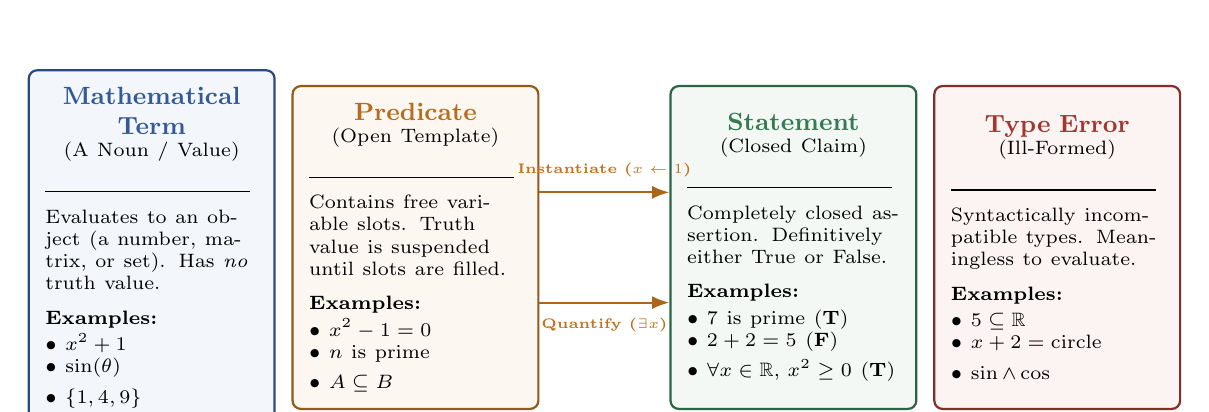
\begin{tikzpicture}[
    font=\small,
    category/.style={draw=#1!70!black, fill=#1!6, rounded corners=3pt, thick, text width=2.7cm, inner sep=6pt, minimum height=4.1cm, align=left},
    header/.style={font=\footnotesize\bfseries\scshape, text=#1!80!black, align=center},
    sample/.style={font=\scriptsize, text=gray!80!black}
]

% Category 1: Terms
\node[category=sourceblue] (col1) at (0, 0) {
    {\centering\textbf{\color{sourceblue!85!black}Mathematical Term}\\\scriptsize(A Noun / Value)\par}
    \vspace{0.2em}
    \rule{2.6cm}{0.4pt}\\[0.35em]
    \scriptsize Evaluates to an object (a number, matrix, or set). Has \emph{no} truth value.\\[0.55em]
    \textbf{Examples:}\\[0.2em]
    $\bullet$~$x^2 + 1$\\
    $\bullet$~$\sin(\theta)$\\
    $\bullet$~$\{1, 4, 9\}$
};

% Category 2: Predicates
\node[category=quotientorange] (col2) at (3.35, 0) {
    {\centering\textbf{\color{quotientorange!85!black}Predicate}\\\scriptsize(Open Template)\par}
    \vspace{0.2em}
    \rule{2.6cm}{0.4pt}\\[0.35em]
    \scriptsize Contains free variable slots. Truth value is suspended until slots are filled.\\[0.55em]
    \textbf{Examples:}\\[0.2em]
    $\bullet$~$x^2 - 1 = 0$\\
    $\bullet$~$n$ is prime\\
    $\bullet$~$A \subseteq B$
};

% Category 3: Statements
\node[category=targetgreen] (col3) at (8.15, 0) {
    {\centering\textbf{\color{targetgreen!85!black}Statement}\\\scriptsize(Closed Claim)\par}
    \vspace{0.2em}
    \rule{2.6cm}{0.4pt}\\[0.35em]
    \scriptsize Completely closed assertion. Definitively either True or False.\\[0.55em]
    \textbf{Examples:}\\[0.2em]
    $\bullet$~$7$ is prime (\textbf{T})\\
    $\bullet$~$2 + 2 = 5$ (\textbf{F})\\
    $\bullet$~$\forall x \in \R,\, x^2 \ge 0$ (\textbf{T})
};

% Category 4: Type Errors
\node[category=trapred] (col4) at (11.5, 0) {
    {\centering\textbf{\color{trapred!85!black}Type Error}\\\scriptsize(Ill-Formed)\par}
    \vspace{0.2em}
    \rule{2.6cm}{0.4pt}\\[0.35em]
    \scriptsize Syntactically incompatible types. Meaningless to evaluate.\\[0.55em]
    \textbf{Examples:}\\[0.2em]
    $\bullet$~$5 \subseteq \R$\\
    $\bullet$~$x + 2 = \text{circle}$\\
    $\bullet$~$\sin \land \cos$
};

% Transformation arrows from Predicate to Statement in dedicated corridor
\draw[-{Latex[length=2.2mm]}, thick, quotientorange!80!black] ([yshift=0.7cm]col2.east) -- node[above=2pt, font=\tiny\bfseries, text=quotientorange!90!black]{Instantiate ($x \leftarrow 1$)} ([yshift=0.7cm]col3.west);
\draw[-{Latex[length=2.2mm]}, thick, quotientorange!80!black] ([yshift=-0.7cm]col2.east) -- node[below=2pt, font=\tiny\bfseries, text=quotientorange!90!black]{Quantify ($\exists x$)} ([yshift=-0.7cm]col3.west);

\end{tikzpicture}
\end{center}

\subsection{Predicates: sentences with empty sockets}

An expression such as $x^2 - 1 = 0$ looks like a statement, but it is not. You cannot say whether it is true or false until you know what $x$ is. If $x = 1$, the sentence becomes $1^2 - 1 = 0$, which is true. If $x = 3$, the sentence becomes $3^2 - 1 = 0$, which is false.

\begin{definition}
A \emph{predicate} is a sentence containing one or more variables that becomes a statement whenever each variable is replaced by a specific element from a specified domain, or bound by a quantifier.
\end{definition}

In computer science, a predicate is a function that returns a boolean value:
\begin{center}
\texttt{isEven : Integer $\to$ \{True, False\}}
\end{center}
Until you pass an input into \texttt{isEven(n)}, the function call produces no boolean output. In mathematics, we write $P(x)$ to indicate that $P$ is a predicate waiting for an input $x$.

\subsection{The domain changes everything}

When you work with a predicate, the mathematical universe from which variables may be chosen---the \emph{domain of discourse}---is not an optional footnote. It governs the truth of the sentence.

Recall our standard number systems:
\begin{itemize}
\item $\N = \{1, 2, 3, \ldots\}$: the natural numbers (positive integers).
\item $\Z = \{\ldots, -2, -1, 0, 1, 2, \ldots\}$: the integers.
\item $\Q = \{p/q : p, q \in \Z, q \neq 0\}$: the rational numbers (fractions).
\item $\R$: the real numbers (including rationals and irrationals like $\sqrt{2}$ and $\pi$).
\item $\C = \{a + bi : a, b \in \R, i^2 = -1\}$: the complex numbers.
\end{itemize}

Now examine the predicate $P(x) : x^2 < 2$. Its truth depends entirely on where $x$ is allowed to live:
\begin{itemize}
\item Over the natural numbers $\N$, the statement ``$\exists x \in \N, x^2 < 2$'' has only a single witness: $x = 1$.
\item Over the integers $\Z$, the solutions are $x \in \{-1, 0, 1\}$.
\item Over the rational numbers $\Q$, there are infinitely many solutions, yet the boundary points $-\sqrt{2}$ and $\sqrt{2}$ do not exist inside $\Q$.
\item Over the real numbers $\R$, the solution set is the open interval $(-\sqrt{2}, \sqrt{2})$.
\item Over the complex numbers $\C$, the inequality $x^2 < 2$ is not even standardly defined, because the complex numbers do not possess an ordering compatible with arithmetic.
\end{itemize}

\begin{trapbox}
Never leave a variable floating without a declared domain. Writing $x^2 \ge 0$ without specifying the domain is an invitation to confusion. Over $\R$, it is true; over $\C$, choosing $x = i$ gives $i^2 = -1 < 0$.
\end{trapbox}

\subsection{Claims, theorems, and mathematical etiquette}

When mathematicians state assertions they intend to establish, they use conventional labels to communicate the structural role of the result:

\begin{itemize}
\item \textbf{Theorem}: A central, landmark result that anchors a theory (e.g., the Pythagorean Theorem, the Fundamental Theorem of Algebra).
\item \textbf{Proposition}: A solid, standalone result of intermediate significance, worth recording in its own right.
\item \textbf{Lemma}: A stepping-stone result. Lemmas often do the heavy algebraic lifting so that the main theorem can be stated cleanly.
\item \textbf{Corollary}: A direct and immediate consequence of an established theorem, requiring minimal additional effort to verify.
\item \textbf{Conjecture}: A statement believed to be true based on strong evidence or heuristic arguments, but which currently lacks an inescapable proof.
\end{itemize}

These terms are stylistic rather than formal. One author's lemma might be celebrated by later generations as a profound theorem (such as Zorn's Lemma or Gauss's Lemma).

\subsection{What formal grammar unlocked---and its operational limits}

Frege's functional taxonomy unlocked an unprecedented clarity: it permanently separated the object of study (nouns/terms) from the assertions made about it (statements), while providing a rigorous home for open equations through predicates. It protects mathematicians from catastrophic category mistakes, such as trying to assert that a number is a subset, or testing whether an open formula is true without binding its variables.

Yet this grammatical taxonomy has an honest operational limitation: \textbf{it is completely static}. It tells you what an expression is, but it says nothing about how variables behave over the course of a multi-paragraph proof. If a sentence contains an $x$, who chooses its value? Is $x$ an immovable constant given by the problem, an adversarial input you have no power to alter, an object you are free to construct, or a private dummy counter that will vanish at the end of the line? 

Without clear rules governing variable lifetime, visibility, and permissions, even grammatically perfect sentences can lead to circular or invalid proofs. In Chapter~3 (\emph{Variables Have Roles: Fixed, Arbitrary, Chosen, Bound}), we move from static grammar to dynamic execution, mastering the four fundamental roles of variables and the iron laws of lexical scope.

\subsection{Exercises}

Classify each expression below as a term, a predicate, a statement, an instruction, or a grammatical type error:
\begin{enumerate}
\item $2x + 5 = 11$.
\item $2(3) + 5 = 11$.
\item $\cos^2(\theta) + \sin^2(\theta)$.
\item For every real number $x$, $x^2 + 1 > 0$.
\item Let $G$ be a finite group.
\item $3 \in \{1, 2, 3, 4\}$.
\item $\{3\} \in \{1, 2, 3, 4\}$.
\item $\{3\} \subseteq \{1, 2, 3, 4\}$.
\item $\sqrt{-1} \le 4$.
\end{enumerate}

For each of the following predicates, describe two different domains where the predicate yields different sets of solutions:
\begin{enumerate}[resume]
\item $Q(x) : 2x = 7$.
\item $R(x) : x^2 = 2$.
\item $S(x) : x \ge 0$.
\end{enumerate}

\newpage

\section{Variables Have Roles: Fixed, Arbitrary, Chosen, and Bound}
\chapterline

In Chapter~2 (\emph{Mathematical Sentences: Statements, Predicates, and Claims}), we saw that a predicate is an open sentence containing empty slots, like $P(x) \colon \text{``}x\text{ is prime''}$. To evaluate whether the sentence is true or false, those slots must be filled by concrete objects or bound by quantifiers.

In elementary algebra, a variable often represents an unknown number in an equation. You solve $3x + 4 = 19$, isolate $x$, and find $x = 5$, where $x$ represents a specific numerical value.

In proof-based mathematics, variables serve several distinct purposes. Letters in a proof represent different concepts, carry distinct logical permissions, and operate within specific scopes. Conflating these roles is a frequent source of error in proofs.

Consider a beginner trying to prove that every integer $n \ge 2$ has a prime factor:
\begin{quote}
\itshape Flawed attempt: Let $n = 12$. Since $12 = 3 \times 4$ and $3$ is prime, $n$ has a prime factor. Therefore, every integer $n \ge 2$ has a prime factor.
\end{quote}
The arithmetic is correct ($12$ really is $3 \times 4$), yet the argument is invalid. Why? Because when a claim begins ``for every integer $n$,'' the argument must hold for an \emph{arbitrary} integer. One cannot substitute a specific chosen number to prove a universal statement.

To read and write proofs with confidence, you need to recognize which of the four fundamental roles a variable plays in any given sentence.

\begin{historybox}
For most of human history, even elementary algebra was purely rhetorical (written out entirely in words without mathematical symbols). Medieval mathematicians had no notation for unknowns or coefficients; every problem was phrased verbally using terms like \emph{cosa} (the Italian word for ``the thing'') and \emph{census} (``the square''). In 1591, the French mathematician Fran\c{c}ois Vi\`ete made a major leap in \emph{In artem analyticem isagoge} by systematically using letters: vowels ($A, E, I$) for unknown quantities and consonants ($B, C, D$) for known parameters. For the first time, mathematicians could manipulate entire families of equations at once.

Yet introducing letters created a stubborn misconception that lasted for two centuries. In the 1700s, Leonhard Euler, Jean le Rond d'Alembert, and Daniel Bernoulli often treated variables as physical quantities that ``flow with time''---an intuition inherited from Isaac Newton's calculus of fluxions (Newton's term for the rates of change of quantities flowing continuously through time). This confusion erupted in the famous vibrating string controversy of 1747--1755, where d'Alembert, Euler, and Bernoulli argued bitterly over the motion of a plucked violin string. Because they lacked a precise definition of a function and had no formal rules for whether a letter was an arbitrary fixed input or an actively moving quantity, they frequently treated a variable as fixed in one step and varied it in the next, falling into contradictory results.

Between 1889 and 1895, the Italian mathematician Giuseppe Peano, together with Gottlob Frege in 1879, dismantled this confusion by formalizing variable binding and lexical scope (the bounded region of text where a variable name is defined and valid). In the 1930s, Alonzo Church introduced the $\lambda$-calculus (lambda calculus, a formal mathematical system where variables are explicitly bound as inputs to functions), which established the scoping rules used by modern programming languages. A variable is neither an unknown number nor a moving physical particle; it is a scoped placeholder governed by strict visibility permissions. Distinguishing the different roles of variables keeps proofs logically sound and avoids variable capture (where an expression accidentally binds a variable with the same name from an outer scope).

Today, an active research challenge in computer science and mathematical logic is how computer proof assistants (such as Lean, Coq, and Isabelle) should manage bound variables when verifying massive libraries of mathematics. Naive substitution causes severe performance bottlenecks. Designing representations that handle variable binding without variable capture---such as De Bruijn indices (numbering placeholders by how many nested scopes enclose them rather than naming them with letters) or nominal logic---remains a lively subject.
\end{historybox}

\subsection{The four roles of variables}

\begin{center}
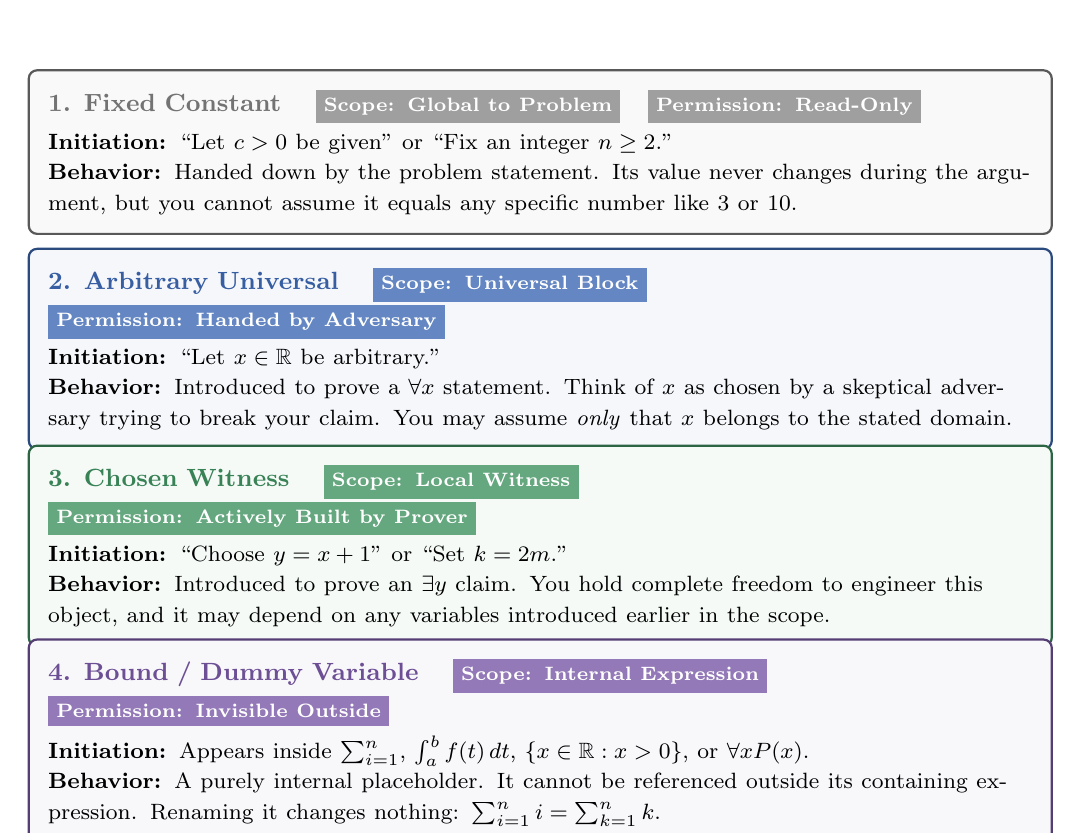
\begin{tikzpicture}[
    font=\small,
    lane/.style={draw=#1!70!black, fill=#1!5, rounded corners=3pt, thick, text width=12.5cm, inner sep=7pt},
    badge/.style={font=\scriptsize\bfseries\scshape, text=white, fill=#1!80!black, rounded corners=2pt, inner sep=3pt}
]

% Lane 1: Fixed Constant
\node[lane=gray] (l1) at (0, 7.5) {
    \textbf{\color{gray!90!black}1. Fixed Constant} \quad \colorbox{gray!75}{\color{white}\scriptsize\bfseries Scope: Global to Problem} \hspace{0.4em} \colorbox{gray!75}{\color{white}\scriptsize\bfseries Permission: Read-Only}\\[0.3em]
    \footnotesize
    \textbf{Initiation:} ``Let $c > 0$ be given'' or ``Fix an integer $n \ge 2$.''\\
    \textbf{Behavior:} Handed down by the problem statement. Its value never changes during the argument, but you cannot assume it equals any specific number like $3$ or $10$.
};

% Lane 2: Arbitrary Universal
\node[lane=sourceblue] (l2) at (0, 5.0) {
    \textbf{\color{sourceblue!90!black}2. Arbitrary Universal} \quad \colorbox{sourceblue!80}{\color{white}\scriptsize\bfseries Scope: Universal Block} \hspace{0.4em} \colorbox{sourceblue!80}{\color{white}\scriptsize\bfseries Permission: Handed by Adversary}\\[0.3em]
    \footnotesize
    \textbf{Initiation:} ``Let $x \in \R$ be arbitrary.''\\
    \textbf{Behavior:} Introduced to prove a $\forall x$ statement. Think of $x$ as chosen by a skeptical adversary trying to break your claim. You may assume \emph{only} that $x$ belongs to the stated domain.
};

% Lane 3: Chosen Witness
\node[lane=targetgreen] (l3) at (0, 2.5) {
    \textbf{\color{targetgreen!90!black}3. Chosen Witness} \quad \colorbox{targetgreen!80}{\color{white}\scriptsize\bfseries Scope: Local Witness} \hspace{0.4em} \colorbox{targetgreen!80}{\color{white}\scriptsize\bfseries Permission: Actively Built by Prover}\\[0.3em]
    \footnotesize
    \textbf{Initiation:} ``Choose $y = x + 1$'' or ``Set $k = 2m$.''\\
    \textbf{Behavior:} Introduced to prove an $\exists y$ claim. You hold complete freedom to engineer this object, and it may depend on any variables introduced earlier in the scope.
};

% Lane 4: Bound Dummy
\node[lane=structurepurple] (l4) at (0, 0.0) {
    \textbf{\color{structurepurple!90!black}4. Bound / Dummy Variable} \quad \colorbox{structurepurple!80}{\color{white}\scriptsize\bfseries Scope: Internal Expression} \hspace{0.4em} \colorbox{structurepurple!80}{\color{white}\scriptsize\bfseries Permission: Invisible Outside}\\[0.3em]
    \footnotesize
    \textbf{Initiation:} Appears inside $\sum_{i=1}^n$, $\int_a^b f(t)\,dt$, $\{x \in \R : x > 0\}$, or $\forall x P(x)$.\\
    \textbf{Behavior:} A purely internal placeholder. It cannot be referenced outside its containing expression. Renaming it changes nothing: $\sum_{i=1}^n i = \sum_{k=1}^n k$.
};

\end{tikzpicture}\\[0.4em]
{\small\textbf{The Four Roles of Variables:} Every letter in a proof serves one of four operational roles. Its category defines where it is visible (scope), who chooses it (permissions), and whether its name can be freely swapped without altering meaning.}
\end{center}

\subsection{Lexical scope: mathematical proofs as programs}

If you have written software, you are already comfortable with variable scope (the region of source code where a name is recognized). A local variable declared inside a function body ceases to exist once that function returns. Trying to access that variable outside the curly braces causes a compile-time error.

Mathematical proofs obey the exact same scoping rules:

\begin{center}
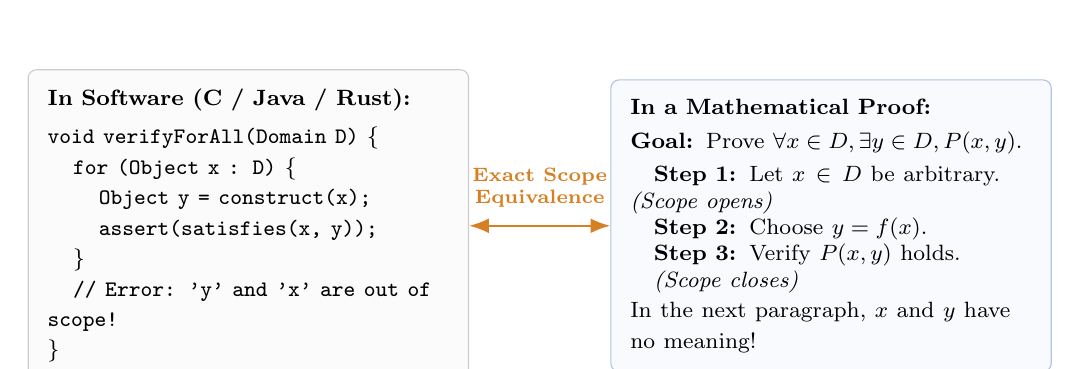
\begin{tikzpicture}[font=\small]

% Code block comparison
\node[draw=gray!40, fill=gray!3, rounded corners=3pt, text width=5.1cm, inner sep=7pt, align=left] (code) at (-3.7, 0) {
    \textbf{\footnotesize In Software (C / Java / Rust):}\\[0.3em]
    \texttt{\footnotesize void verifyForAll(Domain D) \{}\\
    \quad\texttt{\footnotesize for (Object x : D) \{}\\
    \quad\quad\texttt{\footnotesize Object y = construct(x);}\\
    \quad\quad\texttt{\footnotesize assert(satisfies(x, y));}\\
    \quad\texttt{\footnotesize \}}\\
    \quad\texttt{\footnotesize // Error: 'y' and 'x' are out of scope!}\\
    \texttt{\footnotesize \}}
};

% Math block comparison
\node[draw=sourceblue!40, fill=sourceblue!3, rounded corners=3pt, text width=5.1cm, inner sep=7pt, align=left] (math) at (3.7, 0) {
    \textbf{\footnotesize In a Mathematical Proof:}\\[0.3em]
    \footnotesize \textbf{Goal:} Prove $\forall x \in D, \exists y \in D, P(x, y)$.\\[0.3em]
    \quad \textbf{Step 1:} Let $x \in D$ be arbitrary. \emph{(Scope opens)}\\
    \quad \textbf{Step 2:} Choose $y = f(x)$.\\
    \quad \textbf{Step 3:} Verify $P(x, y)$ holds.\\
    \quad \emph{(Scope closes)}\\
    \footnotesize In the next paragraph, $x$ and $y$ have no meaning!
};

\draw[<->, {Latex[length=2.5mm]}-{Latex[length=2.5mm]}, thick, quotientorange] (code.east) -- node[above=3pt, font=\scriptsize\bfseries, text=quotientorange, align=center]{Exact Scope\\Equivalence} (math.west);

\end{tikzpicture}\\[0.4em]
{\small\textbf{Lexical Scoping in Software and Proof:} In both programming and pure mathematics, local variables declared inside a block vanish as soon as the block terminates. Attempting to use $x$ or $y$ after the universal claim is proved is an out-of-scope error.}
\end{center}

When a proof says ``Let $x \in \R$ be arbitrary,'' it opens a local scope block. Inside that block, $x$ is treated as an immutable object about which nothing is known except that $x \in \R$. Once you show that the desired property holds for that generic $x$, the universal statement $\forall x \in \R, \ldots$ is established, and the scope block closes. You cannot subsequently refer to ``that $x$'' in later arguments.

This scoping discipline protects against a frequent proof error: the leaked variable. Suppose you are asked to prove a property about two even integers, $n$ and $m$. By definition, $n$ is even if there exists an integer $k$ such that $n = 2k$. A common beginner mistake is to write:
\begin{quote}
``Since $n$ is even, $n = 2k$. Since $m$ is even, $m = 2k$.''
\end{quote}
Here, the letter $k$ was a local witness tied specifically to the evenness of $n$. Reusing the exact same variable name for $m$ accidentally forces $n = m$, meaning you are no longer proving the claim for two arbitrary even integers, but only for the special case where both integers are equal! To maintain proper variable scoping, every fresh existential claim requires a fresh variable name: $n = 2k$ and $m = 2j$ for integers $k$ and $j$.

\begin{recoverybox}
\textbf{Mental check: Spotting the scope leak}
A student writes the following argument:
\begin{quote}
``To show that $A \subseteq B$, let $x \in A$ be arbitrary. Since $A \subseteq B$, it follows that $x \in B$. Hence $A \subseteq B$ is proved. Therefore, we have found an element $x$ that belongs to both $A$ and $B$, which proves that $A \cap B \neq \emptyset$.''
\end{quote}
What is the fatal flaw in the student's reasoning?
\\[0.3em]
\emph{Answer:} The variable $x$ was introduced as an arbitrary element strictly inside the temporary scope used to prove $A \subseteq B$. Once $A \subseteq B$ is established, that scope closes and $x$ vanishes. The argument does not show that $A$ contains any elements at all! If $A = \emptyset$, the subset claim $\emptyset \subseteq B$ is vacuously true, yet $\emptyset \cap B = \emptyset$. Claiming that $x \in A \cap B$ in the next sentence attempts to use an out-of-scope variable that has already expired.
\end{recoverybox}

\subsection{Free versus bound variables}

Look at the following three mathematical expressions:
\[
\text{(A)}\quad \sum_{i=1}^n i^2, \qquad\qquad \text{(B)}\quad \int_0^1 x^2 \, dx, \qquad\qquad \text{(C)}\quad x^2 + y^2 = 1.
\]

In expression (A), the index $i$ is \emph{bound} by the summation. The letter $n$, however, is \emph{free}: the numerical value of the sum depends directly on what $n$ is. If you change $n$ from $3$ to $4$, the sum changes from $14$ to $30$. But if you replace every occurrence of $i$ with $j$, getting $\sum_{j=1}^n j^2$, the value is completely unchanged. The index $i$ is merely an internal dummy counter.

In expression (B), the variable $x$ is bound by the integral. The expression evaluates to the concrete number $1/3$. There is no $x$ remaining in the answer. Writing ``let $x = 10$'' before the integral has zero effect on its outcome.

In expression (C), both $x$ and $y$ are free. Without additional context, the equation does not assert a truth value; it defines a predicate (an open condition satisfied by pairs of points on the unit circle).

The distinction between free and bound variables is straightforward: \textbf{free variables are parameters determined by the surrounding context, while bound variables are internal placeholders local to an operator} (Figure~\ref{03:fig-bound-variable-capsule}).

\begin{figure}[htbp]
\centering
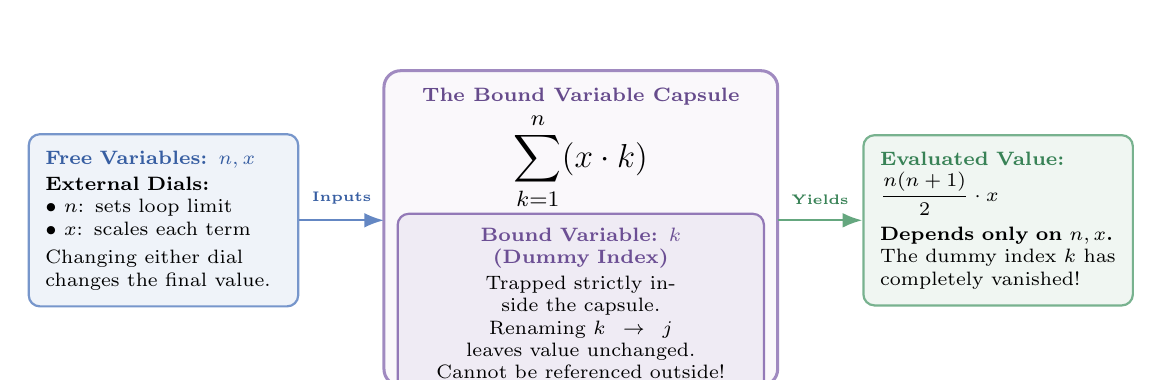
\begin{tikzpicture}[
    font=\small,
    capsule/.style={draw=structurepurple!70, fill=structurepurple!4, rounded corners=6pt, line width=1.1pt},
    freebox/.style={draw=sourceblue!70, fill=sourceblue!8, rounded corners=4pt, thick, align=left, inner sep=6pt},
    boundbox/.style={draw=structurepurple!80, fill=structurepurple!12, rounded corners=4pt, thick, align=center, inner sep=5pt},
    outbox/.style={draw=targetgreen!70, fill=targetgreen!8, rounded corners=4pt, thick, align=left, inner sep=6pt}
]

% Left: Free inputs box
\node[freebox, font=\scriptsize, text width=3.0cm] (freenote) at (-5.3, 0) {
    \textbf{\color{sourceblue!90!black}Free Variables: $n, x$}\\[0.2em]
    \textbf{External Dials:}\\
    $\bullet$~$n$: sets loop limit\\
    $\bullet$~$x$: scales each term\\[0.3em]
    Changing either dial changes the final value.
};

% Capsule container
\draw[capsule] (-2.5, -2.1) rectangle (2.5, 1.9);
\node[anchor=north, font=\scriptsize\bfseries\scshape, text=structurepurple!85!black] at (0, 1.8) {The Bound Variable Capsule};

% Expression inside capsule
\node[font=\large] (expr) at (0, 0.75) {$\displaystyle \sum_{k=1}^n (x \cdot k)$};

% Bound note inside capsule
\node[boundbox, font=\scriptsize, text width=4.3cm] (bnote) at (0, -1.05) {
    \textbf{\color{structurepurple!90!black}Bound Variable: $k$ (Dummy Index)}\\[0.2em]
    Trapped strictly inside the capsule.\\
    Renaming $k \to j$ leaves value unchanged.\\
    Cannot be referenced outside!
};

% Arrow into capsule
\draw[-{Latex[length=2.5mm]}, thick, sourceblue!80] (freenote.east) -- node[above=2pt, font=\tiny\bfseries, text=sourceblue!90!black]{Inputs} (-2.5, 0);

% Right: Output box
\node[outbox, font=\scriptsize, text width=3.0cm] (outnote) at (5.3, 0) {
    \textbf{\color{targetgreen!90!black}Evaluated Value:}\\[0.2em]
    $\displaystyle \frac{n(n+1)}{2} \cdot x$\\[0.4em]
    \textbf{Depends only on $n, x$.}\\
    The dummy index $k$ has completely vanished!
};

% Arrow out of capsule
\draw[-{Latex[length=2.5mm]}, thick, targetgreen!80] (2.5, 0) -- node[above=2pt, font=\tiny\bfseries, text=targetgreen!90!black]{Yields} (outnote.west);

\end{tikzpicture}
\caption{Free and bound variables in an expression. Free variables ($n, x$) are parameters supplied from the surrounding context. The bound variable ($k$) is an internal index local to the summation; it cannot be referenced in the outer scope and disappears upon evaluation.}
\label{03:fig-bound-variable-capsule}
\end{figure}

Because a bound variable is purely internal, you are always free to rename it to any other symbol that is not already in use. In mathematical logic, this principle is called $\alpha$-equivalence (alpha-equivalence, meaning two formulas are identical up to renaming of bound variables):
\[
\int_a^b f(t) \, dt = \int_a^b f(u) \, du = \int_a^b f(w) \, dw.
\]
The choice of letter $t, u, w$ carries zero mathematical information. 

However, you must never rename a bound variable to a letter that is already free in the surrounding context. In the sum $\sum_{k=1}^n k$, renaming $k$ to $n$ produces $\sum_{n=1}^n n$. This name collision triggers \emph{variable capture}: the upper limit $n$ is captured by the summation index, destroying the original formula.

\begin{recoverybox}
\textbf{Mental check: Free or bound?}
In each of the following expressions, identify which letters are free and which are bound:
\begin{enumerate}[label=(\alph*)]
\item $\displaystyle \int_1^x \frac{1}{t} \, dt = \ln(x)$.
\item $\displaystyle \{y \in \R : y^2 < c\}$.
\item $\displaystyle \lim_{h \to 0} \frac{f(x+h) - f(x)}{h}$.
\end{enumerate}
\emph{Answers:} In (a), $x$ is free (it is the upper limit of integration); $t$ is bound by $dt$. In (b), $c$ is free (a parameter); $y$ is bound by the set-builder braces. In (c), $x$ and $f$ are free (the point and the function); $h$ is bound by the limit operator.
\end{recoverybox}

\subsection{A worked example of quantifier and role parsing}

Consider the statement:
\[
\forall x \in \R, \, \exists y \in \R \text{ such that } x + y = 0.
\]

Let us trace the roles and permissions line by line:
\begin{enumerate}
\item \textbf{The universal player moves first}: The statement begins with $\forall x \in \R$. Therefore, in our proof, we must begin by accepting an \emph{arbitrary} real number:
\begin{quote}
``Let $x \in \R$ be arbitrary.''
\end{quote}
We cannot choose $x = 0$ or $x = 5$. We must leave $x$ completely general.
\item \textbf{The existential player responds}: The next quantifier is $\exists y \in \R$. We must now produce a \emph{chosen witness}. Because $y$ comes \emph{after} $x$ in the quantifier order, our choice of $y$ is legally permitted to depend on $x$:
\begin{quote}
``Choose $y = -x$.''
\end{quote}
\item \textbf{Verify the requirements}: We verify two things: first, that $-x \in \R$ (it is, since the real numbers are closed under negation), and second, that $x + y = x + (-x) = 0$.
\item \textbf{Conclude and close scope}: Both conditions are satisfied, so the statement is proved, and the local variables $x$ and $y$ close their scopes.
\end{enumerate}

Now observe what happens if the quantifiers are reversed:
\[
\exists y \in \R \text{ such that } \forall x \in \R, \, x + y = 0.
\]
Here, $y$ must be chosen \emph{first}, independently of $x$. Any proposed value of $y$ (say $y = 0$) fails for $x = 1$, since $1 + 0 = 1 \neq 0$. In fact, for any fixed real number $y$, choosing $x = -y + 1$ yields $x + y = (-y + 1) + y = 1 \neq 0$. Reversing the quantifier order changes the dependence between the variables.

\begin{trapbox}
Never define an existential witness using a variable that has not yet entered scope. In the statement $\forall x \, \exists y$, your formula for $y$ may use $x$. In $\exists y \, \forall x$, your formula for $y$ must be an absolute constant chosen before $x$ is announced. Writing ``Choose $y = -x$'' before $\forall x$ has appeared is an illegal forward reference.
\end{trapbox}

\subsection{The bridge to quantifiers: who moves first?}

Scoping rules tell us where a variable is visible and what operations are legally permitted on it. But in advanced mathematics, theorems rarely involve a single variable in isolation. They involve chains of variables interacting with one another.

When you prove a theorem in analysis or algebra, you often handle several variables at once: a fixed space, an arbitrary element, a chosen witness, and a bound index. Who chooses which letter, and which choices may depend on earlier ones?

In Chapter~4 (\emph{Quantifiers: The Game of For Every and There Exists}), we examine how quantifiers ($\forall$ and $\exists$) govern these choices as a game, and why their order is critical to mathematical statements.

\subsection{Exercises}

\begin{enumerate}
\item \textbf{Role Identification (Warm-up):} In the statement
\[
\forall n \in \Z, \, \exists m \in \Z \text{ such that } n = 2m + 1,
\]
identify the roles of $n$ and $m$. Is the statement true or false? Notice that even if a statement is mathematically false, its variables still possess well-defined syntactic roles!

\item \textbf{Multi-Variable Parsing (Calculus):} In the definition of continuity of a function $f \colon \R \to \R$ at a point $c$:
\begin{quote}
``For every $\eps > 0$, there exists $\delta > 0$ such that for all $x \in \R$, if $|x - c| < \delta$, then $|f(x) - f(c)| < \eps$,''
\end{quote}
identify the exact role of each letter: $c$, $\eps$, $\delta$, and $x$. Which variable is a fixed constant, which are arbitrary universals, and which is a chosen witness? On which prior variables is the formula for $\delta$ permitted to depend?

\item \textbf{Bound Dummies and Evaluation:} In the expression
\[
L = \lim_{n \to \infty} \sum_{k=1}^n \frac{k}{n^2}:
\]
\begin{enumerate}[label=(\alph*)]
\item Which variables are bound dummies, and what binding operator captures each of them?
\item Compute the value of the expression by first summing $\sum_{k=1}^n k = \frac{n(n+1)}{2}$ and then evaluating the limit as $n \to \infty$. Does any variable survive into the final number?
\end{enumerate}

\item \textbf{Diagnosing Proof Bugs (Illegal Specialization):} Explain the exact error in the following pseudo-proof:
\begin{quote}
\itshape Claim: Every integer is even.\\
False proof: Let $n \in \Z$ be arbitrary. Choose $n = 4$. Since $4 = 2(2)$, $n$ is even. Therefore every integer is even.
\end{quote}
Which role permission was violated? Why does setting $n = 4$ destroy the universal validity of the proof?

\item \textbf{Diagnosing Proof Bugs (Forward Referencing):} Explain what is wrong with the following proof attempt:
\begin{quote}
\itshape Claim: $\exists y \in \R \text{ such that } \forall x \in \R, \, x + y = x$.\\
False proof: Let $x \in \R$ be arbitrary. Choose $y = x - x = 0$. Since $x + 0 = x$, the number $y$ works for all $x$. Therefore such a $y$ exists.
\end{quote}
Although the claim is actually true (the number $0$ indeed works for all $x$), why is this proof invalid as written? (Look at the quantifier order and the scope-opening line).

\item \textbf{Variable Capture in Calculus:} Consider the function $F(x) = \int_0^x (x - t) \, dt$.
\begin{enumerate}[label=(\alph*)]
\item Evaluate $F(x)$ by integrating with respect to $t$.
\item A student reasons: ``Because $t$ is a dummy variable, I can rename it to $x$. Then the integrand becomes $(x - x) = 0$, so $\int_0^x 0 \, dx = 0$.'' Explain why this reasoning is completely false, identifying the exact collision between a free variable and a bound variable.
\end{enumerate}

\item \textbf{Proof Lab (Writing Scopes Explicitly):} Write a rigorous, step-by-step proof of the claim:
\[
\forall x \in \R, \, (x > 3 \implies x^2 - 9 > 0).
\]
For each line of your proof, explicitly state whether you are opening a scope, introducing an arbitrary element, assuming a hypothesis, or closing a scope.
\end{enumerate}

\begin{walkbox}
When reading an advanced textbook, pause at each variable. Ask yourself: ``Is this a fixed parameter, an arbitrary element of a set, a chosen witness satisfying an existential claim, or a bound index local to an expression?''
\end{walkbox}

\newpage

\section{Quantifiers: The Game of For Every and There Exists}
\chapterline

In Chapter~3, we saw that variables in mathematics serve distinct logical roles: an \emph{arbitrary} variable represents any generic element of a domain, while a \emph{chosen} variable is a specific witness constructed to establish an existential claim.

Yet in mathematical statements, variables do not appear only in isolation. They appear in pairs, triplets, and chains. When multiple variables interact in the same claim, who sets the terms first? Which variable choices may depend on earlier ones?

The answer is governed by two symbols called \textbf{quantifiers}---operators that specify \emph{how many} elements in a collection satisfy a given property:
\[
\forall \quad \text{(``for every'' / ``for all'')}, \qquad\qquad \exists \quad \text{(``there exists'' / ``for at least one'')}.
\]
The order in which these symbols appear determines the logical structure of a proof. Reversing two quantifiers is not a minor syntactic detail; it frequently transforms a true theorem into a false statement.

\begin{historybox}
In the early nineteenth century, Augustin-Louis Cauchy was striving to put calculus on solid ground. Working in 1821 with informal notions of limits, Cauchy stated in his \emph{Cours d'Analyse} that the sum of any convergent series of continuous functions must be continuous. However, Joseph Fourier had already observed that trigonometric series of sines and cosines could converge to discontinuous functions, such as square waves. For decades, mathematicians debated how a sum of continuous terms could yield a discontinuous limit.

The contradiction was resolved in 1847 when Philipp Ludwig von Seidel and George Gabriel Stokes independently realized that Cauchy had conflated two different orders of quantifiers. If you pick any single point on the horizontal axis, the sequence of functions may settle down at that specific point ($\forall x \, \exists N$, known as \emph{pointwise convergence}). That does not guarantee that the sequence settles down at the same rate across the entire domain ($\exists N \, \forall x$, formalized by Karl Weierstrass as \emph{uniform convergence}).

When Gottlob Frege (1879) and Charles Sanders Peirce (1885) invented explicit symbolic notation for quantifiers, this linguistic ambiguity vanished. Quantifiers gave mathematicians the precision to distinguish pointwise convergence from uniform convergence. Alternating quantifiers remain central in modern logic and theoretical computer science: the \emph{Polynomial Hierarchy} classifies computational problems by how many alternating $\forall$ and $\exists$ decisions they require. Whether adding more quantifier alternations strictly expands the class of solvable problems, or whether the hierarchy collapses to a finite level, remains a fundamental open problem in complexity theory.
\end{historybox}

To see why quantifier order is essential, it helps to view quantified statements through game-theoretic semantics, where truth is evaluated as an interaction between two participants.

\subsection{Quantifiers as a two-player game}

Imagine a game played on a mathematical domain between two players:
\begin{itemize}
\item \textbf{The Universal Challenger ($\forall$)}: A challenger seeking a counterexample to the claim. Whenever a statement specifies $\forall x$, the Challenger selects an element $x$ from the domain in an attempt to make the condition fail.
\item \textbf{The Existential Prover ($\exists$)}: The prover attempting to verify the claim. Whenever a statement specifies $\exists y$, the Prover must produce an element $y$ that satisfies the required condition.
\end{itemize}

The fundamental rule of this game is simple: \textbf{the order of the quantifiers dictates the order of play}. Whoever appears first moves first. Whoever moves second plays with full knowledge of the first player's move.

\subsection{Pointwise dependence versus uniform choice}

Let us compare these two roles on the real numbers $\R$ with the relation $x + y = 0$.

\textbf{Game 1}: $\forall x \in \R, \, \exists y \in \R \text{ such that } x + y = 0$.
\begin{itemize}
\item The Challenger plays first, choosing any real number $x$.
\item You play second. Given their choice of $x$, you respond with $y = -x$.
\item Check the condition: $x + (-x) = 0$. Because you can produce a valid $y$ for any $x$ the Challenger selects, the statement is \textbf{True}.
\end{itemize}

\textbf{Game 2}: $\exists y \in \R \text{ such that } \forall x \in \R, \, x + y = 0$.
\begin{itemize}
\item You must play first: you must choose a single real number $y$ before the Challenger reveals their move.
\item Suppose you choose $y = 0$.
\item The Challenger now plays second, inspecting your $y$. Knowing your choice is $0$, they pick $x = 5$.
\item Check the condition: $5 + 0 = 5 \neq 0$.
\item Can any choice of $y$ work? No: for any fixed $y$, the Challenger simply picks $x = 1 - y$, forcing $x + y = 1 \neq 0$. The statement is \textbf{False}.
\end{itemize}

In Game 1, the choice of $y$ depends on $x$: your response can vary with each input. In Game 2, you must select a single uniform value of $y$ that works for every possible $x$.

\begin{recoverybox}
\textbf{Mental check:} What happens if we change the domain of Game~1 from the real numbers $\R$ to the natural numbers $\N = \{1, 2, 3, \ldots\}$?
\[
\forall x \in \N, \, \exists y \in \N \text{ such that } x + y = 0.
\]
Can the Prover still win?
\emph{Answer:} No. The Challenger picks $x = 1$. The only real number satisfying $1 + y = 0$ is $y = -1$, but $-1 \notin \N$. No such natural number exists, so the statement is False. The domain of a quantifier limits the allowable choices for each variable.
\end{recoverybox}

\subsection{Visualizing the game on a grid}

We can make this distinction visible on a grid where rows represent inputs chosen by the Challenger ($x$) and columns represent responses chosen by the Prover ($y$). A cell $(x, y)$ is lit up whenever the predicate $P(x, y)$---a mathematical condition whose truth depends on the pair $(x, y)$---is satisfied.

\begin{center}
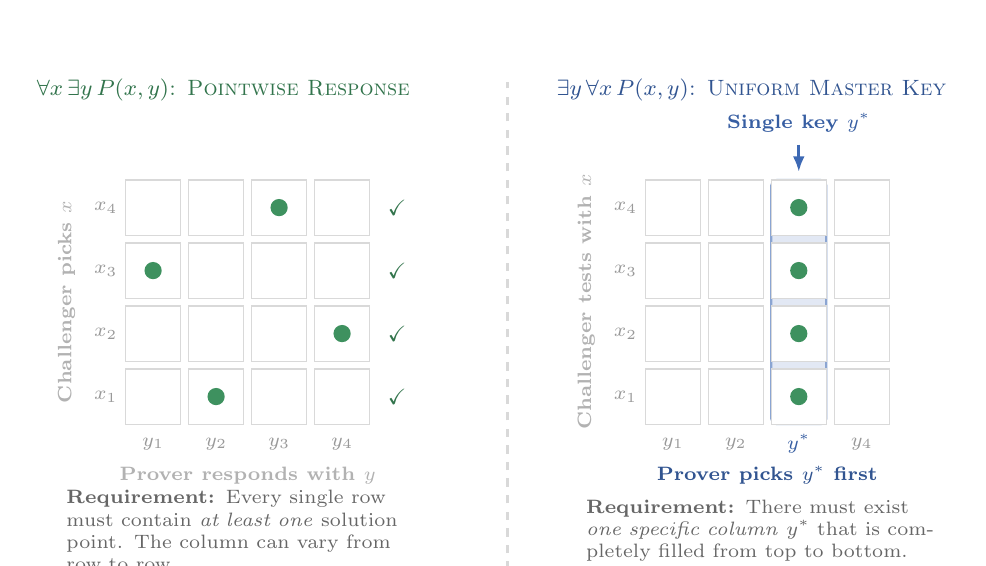
\begin{tikzpicture}[
    font=\small,
    cell/.style={draw=gray!30, fill=white, minimum size=0.7cm, inner sep=0pt},
    hitpoint/.style={circle, fill=targetgreen, inner sep=2.2pt},
    mastercol/.style={fill=sourceblue!15, draw=sourceblue!60, thick}
]

% Panel A: Forall x Exists y
\begin{scope}[xshift=0cm]
    \node[anchor=west, font=\footnotesize\scshape, text=targetgreen!80!black] at (-0.8, 4.7) {$\forall x \, \exists y \, P(x,y)$: Pointwise Response};
    
    % Axis role labels
    \node[font=\scriptsize\bfseries, text=gray!60, rotate=90] at (-0.3, 2.0) {Challenger picks $x$};
    \node[font=\scriptsize\bfseries, text=gray!60] at (2.0, -0.2) {Prover responds with $y$};

    % Grid background
    \foreach \r in {1,2,3,4} {
        \foreach \c in {1,2,3,4} {
            \node[cell] at (\c*0.8, \r*0.8) {};
        }
    }
    
    % Axis labels
    \node[font=\scriptsize, text=gray!80] at (0.2, 3.2) {$x_4$};
    \node[font=\scriptsize, text=gray!80] at (0.2, 2.4) {$x_3$};
    \node[font=\scriptsize, text=gray!80] at (0.2, 1.6) {$x_2$};
    \node[font=\scriptsize, text=gray!80] at (0.2, 0.8) {$x_1$};
    
    \node[font=\scriptsize, text=gray!80] at (0.8, 0.2) {$y_1$};
    \node[font=\scriptsize, text=gray!80] at (1.6, 0.2) {$y_2$};
    \node[font=\scriptsize, text=gray!80] at (2.4, 0.2) {$y_3$};
    \node[font=\scriptsize, text=gray!80] at (3.2, 0.2) {$y_4$};
    
    % Green hits: at least one per row
    \node[hitpoint] at (1.6, 0.8) {}; % (x1, y2)
    \node[hitpoint] at (3.2, 1.6) {}; % (x2, y4)
    \node[hitpoint] at (0.8, 2.4) {}; % (x3, y1)
    \node[hitpoint] at (2.4, 3.2) {}; % (x4, y3)
    
    % Row indicators: green checkmarks
    \foreach \r in {0.8, 1.6, 2.4, 3.2} {
        \node[font=\footnotesize, text=targetgreen!80!black] at (3.9, \r) {$\checkmark$};
    }
    
    \node[text width=4.6cm, align=left, font=\scriptsize, text=gray!80!black] at (2.0, -0.9) {
        \textbf{Requirement:} Every single row must contain \emph{at least one} solution point. The column can vary from row to row.
    };
\end{scope}

% Divider line
\draw[draw=gray!30, dashed, thick] (5.3, -1.4) -- (5.3, 4.8);

% Panel B: Exists y Forall x
\begin{scope}[xshift=6.6cm]
    \node[anchor=west, font=\footnotesize\scshape, text=sourceblue!80!black] at (-0.8, 4.7) {$\exists y \, \forall x \, P(x,y)$: Uniform Master Key};
    
    % Axis role labels
    \node[font=\scriptsize\bfseries, text=gray!60, rotate=90] at (-0.3, 2.0) {Challenger tests with $x$};
    \node[font=\scriptsize\bfseries, text=sourceblue!80!black] at (2.0, -0.2) {Prover picks $y^*$ first};

    % Highlighted master column y3
    \draw[mastercol, rounded corners=2pt] (2.05, 0.45) rectangle (2.75, 3.55);
    
    % Grid background
    \foreach \r in {1,2,3,4} {
        \foreach \c in {1,2,3,4} {
            \node[cell] at (\c*0.8, \r*0.8) {};
        }
    }
    
    % Axis labels
    \node[font=\scriptsize, text=gray!80] at (0.2, 3.2) {$x_4$};
    \node[font=\scriptsize, text=gray!80] at (0.2, 2.4) {$x_3$};
    \node[font=\scriptsize, text=gray!80] at (0.2, 1.6) {$x_2$};
    \node[font=\scriptsize, text=gray!80] at (0.2, 0.8) {$x_1$};
    
    \node[font=\scriptsize, text=gray!80] at (0.8, 0.2) {$y_1$};
    \node[font=\scriptsize, text=gray!80] at (1.6, 0.2) {$y_2$};
    \node[font=\scriptsize\bfseries, text=sourceblue!90!black] at (2.4, 0.2) {$y^*$};
    \node[font=\scriptsize, text=gray!80] at (3.2, 0.2) {$y_4$};
    
    % Green hits all down column 3
    \node[hitpoint] at (2.4, 0.8) {};
    \node[hitpoint] at (2.4, 1.6) {};
    \node[hitpoint] at (2.4, 2.4) {};
    \node[hitpoint] at (2.4, 3.2) {};
    
    % Column indicator
    \draw[-{Latex[length=2mm]}, very thick, sourceblue] (2.4, 4.0) -- (2.4, 3.65);
    \node[above=1pt, font=\scriptsize\bfseries, text=sourceblue!90!black] at (2.4, 4.0) {Single key $y^*$};
    
    \node[text width=4.6cm, align=left, font=\scriptsize, text=gray!80!black] at (2.0, -0.9) {
        \textbf{Requirement:} There must exist \emph{one specific column} $y^*$ that is completely filled from top to bottom.
    };
\end{scope}

\end{tikzpicture}
\end{center}

Notice the visual distinction:
\begin{itemize}
\item To satisfy $\forall x \, \exists y \, P(x, y)$, at least one point in each row must be satisfied, even if the column varies from row to row.
\item To satisfy $\exists y \, \forall x \, P(x, y)$, an entire single column must be completely filled.
\end{itemize}

This is why $\exists y \, \forall x \, P(x, y)$ is a much stronger assertion than $\forall x \, \exists y \, P(x, y)$. In fact, the implication:
\[
\bigl(\exists y \, \forall x \, P(x, y)\bigr) \implies \bigl(\forall x \, \exists y \, P(x, y)\bigr)
\]
is always universally valid (if you have an unbroken column, every row clearly contains a point in that column).

Why is this implication guaranteed to hold? We can verify it directly using the variable roles introduced in Chapter~3:
\begin{enumerate}
\item \textbf{Assume the premise:} We assume that $\exists y \, \forall x \, P(x, y)$ is true. By the definition of existence, there is some specific witness $y^* \in D$ such that $P(x, y^*)$ holds for every $x \in D$.
\item \textbf{Set up the goal:} We need to prove $\forall x \, \exists y \, P(x, y)$. Following our game, let $x \in D$ be arbitrary (the Challenger hands us an element).
\item \textbf{Choose the response:} We must produce a winning response $y$. Which element do we pick? We choose $y = y^*$.
\item \textbf{Verify:} Does $P(x, y^*)$ hold? Yes, because $P(x, y^*)$ holds for \emph{all} elements in the domain, including the arbitrary $x$ handed to us.
\end{enumerate}
The reverse implication, however, is not generally true: having winning points in different rows does not mean they align in a single column.

\subsection{How the game dictates proof structure}

Quantifiers directly determine the logical skeleton of a proof (Figure~\ref{04:fig-proof-skeletons}):

\begin{figure}[htbp]
\centering
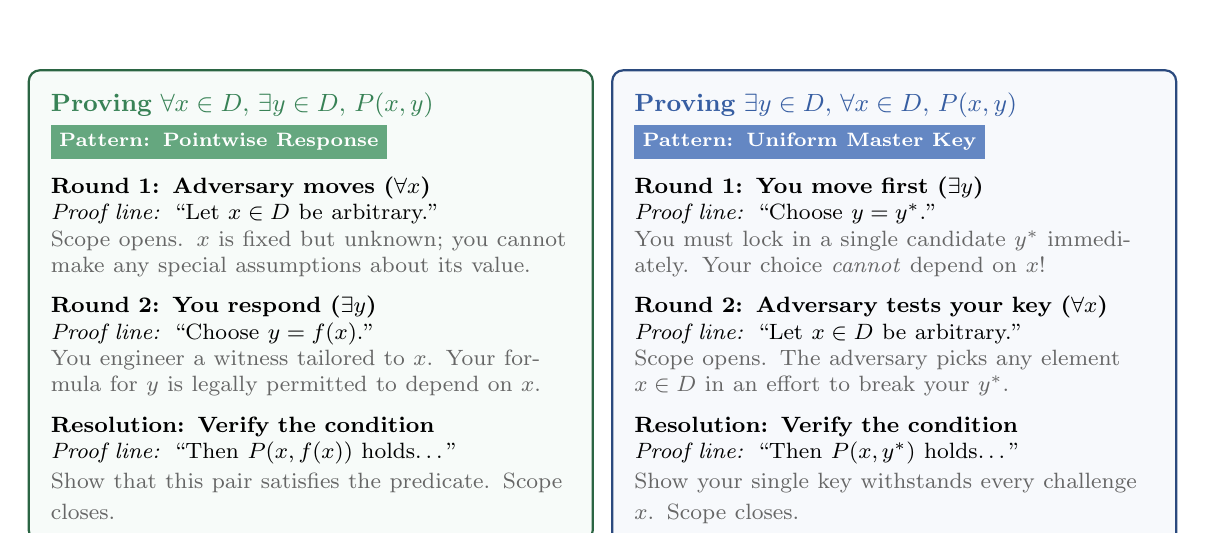
\begin{tikzpicture}[
    font=\small,
    proofcard/.style={draw=#1!70!black, fill=#1!4, rounded corners=4pt, thick, text width=6.6cm, inner sep=8pt}
]

% Left Card: Pointwise
\node[proofcard=targetgreen, anchor=north west] (cardA) at (0, 0) {
    \textbf{\color{targetgreen!90!black}Proving $\forall x \in D, \, \exists y \in D, \, P(x, y)$}\\[0.2em]
    \colorbox{targetgreen!80}{\color{white}\scriptsize\bfseries Pattern: Pointwise Response}\\[0.6em]
    \footnotesize
    \textbf{Round 1: Adversary moves ($\forall x$)}\\
    \emph{Proof line:} ``Let $x \in D$ be arbitrary.''\\
    \color{gray!80!black}Scope opens. $x$ is fixed but unknown; you cannot make any special assumptions about its value.\\[0.6em]
    \color{black}
    \textbf{Round 2: You respond ($\exists y$)}\\
    \emph{Proof line:} ``Choose $y = f(x)$.''\\
    \color{gray!80!black}You engineer a witness tailored to $x$. Your formula for $y$ is legally permitted to depend on $x$.\\[0.6em]
    \color{black}
    \textbf{Resolution: Verify the condition}\\
    \emph{Proof line:} ``Then $P(x, f(x))$ holds\dots''\\
    \color{gray!80!black}Show that this pair satisfies the predicate. Scope closes.
};

% Right Card: Uniform
\node[proofcard=sourceblue, anchor=north east] (cardB) at (14.6, 0) {
    \textbf{\color{sourceblue!90!black}Proving $\exists y \in D, \, \forall x \in D, \, P(x, y)$}\\[0.2em]
    \colorbox{sourceblue!80}{\color{white}\scriptsize\bfseries Pattern: Uniform Master Key}\\[0.6em]
    \footnotesize
    \textbf{Round 1: You move first ($\exists y$)}\\
    \emph{Proof line:} ``Choose $y = y^*$.''\\
    \color{gray!80!black}You must lock in a single candidate $y^*$ immediately. Your choice \emph{cannot} depend on $x$!\\[0.6em]
    \color{black}
    \textbf{Round 2: Adversary tests your key ($\forall x$)}\\
    \emph{Proof line:} ``Let $x \in D$ be arbitrary.''\\
    \color{gray!80!black}Scope opens. The adversary picks any element $x \in D$ in an effort to break your $y^*$.\\[0.6em]
    \color{black}
    \textbf{Resolution: Verify the condition}\\
    \emph{Proof line:} ``Then $P(x, y^*)$ holds\dots''\\
    \color{gray!80!black}Show your single key withstands every challenge $x$. Scope closes.
};

\end{tikzpicture}
\caption{Proof skeletons determined by quantifier order. In a $\forall x \, \exists y$ statement (left), the universal variable is introduced first and the existential witness may depend on $x$. In an $\exists y \, \forall x$ statement (right), the prover must produce a single witness $y^*$ that works for every $x$.}
\label{04:fig-proof-skeletons}
\end{figure}

\begin{recoverybox}
\textbf{Mental check:} In a proof of $\forall x \in \R, \, \exists y \in \R, \, P(x, y)$, can your definition of $y$ mention $x$? Can it mention a variable $z$ that has never been introduced?
\emph{Answer:} Yes to $x$, because $x$ was introduced in an outer scope before $y$ was chosen. No to $z$, because $z$ does not exist in the current scope. Variable scoping in proofs is just as strict as in computer programs.
\end{recoverybox}

\subsection{When can quantifiers swap? (Homogeneous vs.\ heterogeneous)}

Does quantifier order always matter? Not quite. The order matters only when you \textbf{switch players}:
\begin{itemize}
\item \textbf{Homogeneous quantifiers commute:}
\[
\forall x \, \forall y \, P(x, y) \iff \forall y \, \forall x \, P(x, y), \qquad\qquad \exists x \, \exists y \, P(x, y) \iff \exists y \, \exists x \, P(x, y).
\]
When both quantifiers are $\forall$, the Challenger chooses both elements. It makes no difference whether they pick $x$ first or $y$ first; their goal is simply to find any pair $(x, y)$ that breaks the claim. We often abbreviate this as $\forall x, y \in D$. Similarly, when both quantifiers are $\exists$, you get to pick both witnesses together.
\item \textbf{Heterogeneous quantifiers do not commute:}
\[
\forall x \, \exists y \, P(x, y) \not\iff \exists y \, \forall x \, P(x, y).
\]
As soon as $\forall$ and $\exists$ alternate, the game becomes asymmetric. Whoever moves second enjoys an information advantage: they get to inspect the first player's move before committing to their own.
\end{itemize}

\subsection{Everyday, software, and engineering analogies}

The distinction between $\forall x \, \exists y$ and $\exists y \, \forall x$ appears throughout technology and daily life.

\textbf{1. An audio amplifier specification:}
\begin{quote}
\textbf{Claim A}: For every frequency $f \in [20\,\text{Hz}, 20\,\text{kHz}]$, there exists an equalization filter setting that cancels distortion.
\end{quote}
This is a standard feature. The user turns a dial tailored to the specific problematic frequency. The setting responds to the frequency: $\text{setting} = g(f)$.

Now compare:
\begin{quote}
\textbf{Claim B}: There exists a single equalization filter setting that cancels distortion at every frequency $f \in [20\,\text{Hz}, 20\,\text{kHz}]$.
\end{quote}
This is a far more demanding engineering requirement. It demands a single static circuit that simultaneously eliminates all distortion across the whole audio spectrum.

\textbf{2. Software algorithms:}
\begin{itemize}
\item \emph{Pointwise:} ``For every input list $L$, there exists a Python script that sorts $L$ in $O(n)$ time.'' This is trivially true: if $L$ is already sorted, a simple verification script runs in linear time; if $L$ is in reverse order, a reverse-reading script works. You pick a custom script after inspecting the list!
\item \emph{Uniform:} ``There exists a comparison-based Python script that sorts every input list $L$ in $O(n)$ time.'' This is mathematically impossible: the famous comparison-sorting lower bound proves that any single comparison sort requires $\Omega(n \log n)$ operations in the worst case.
\end{itemize}

\textbf{3. Human language ambiguities:}
In everyday conversation, English often blurs quantifier order. If someone says ``Everyone loves someone,'' do they mean that each person has their own favorite companion ($\forall p \, \exists s$), or that there is a single beloved celebrity whom everyone admires ($\exists s \, \forall p$)? Mathematical notation exists precisely to prevent such ambiguities from corrupting our reasoning.

\begin{focusbox}
Whenever you read a definition with nested quantifiers, look at which variable appears first. A variable introduced later may depend on variables introduced earlier; a variable introduced earlier must be chosen independently of those that follow.
\end{focusbox}

\subsection{Three nested quantifiers and the bridge to negation}

The two-player game scales naturally to three, four, or any number of quantifiers: the players simply alternate turns.

Consider the definition of a \textbf{bounded function} $f \colon \R \to \R$ (a function whose values remain within a bounded interval):
\[
\exists M \in \R \text{ such that } \forall x \in \R, \, |f(x)| \le M.
\]
Here, you (the Prover) must move first by proposing a bound $M$. The Challenger then inspects your $M$ and tests whether any $x \in \R$ violates the bound. For $f(x) = \sin(x)$, you succeed by choosing $M = 1$. For $f(x) = x^2$, whatever $M$ you pick, the Challenger counters with $x = \sqrt{M} + 1$, so the function is unbounded.

Or consider the formal definition of the \textbf{limit of a sequence} $a_n \to L$:
\[
\forall \eps > 0, \, \exists N \in \N, \, \forall n \ge N, \, |a_n - L| < \eps.
\]
This corresponds to three rounds:
\begin{enumerate}
\item \textbf{Round 1 (Challenger, $\forall \eps > 0$):} Demands a tolerance, such as $\eps = 0.001$.
\item \textbf{Round 2 (Prover, $\exists N \in \N$):} Responds with a cutoff index $N$ computed from $\eps$.
\item \textbf{Round 3 (Challenger, $\forall n \ge N$):} Tests any subsequent term $n \ge N$ to see if $|a_n - L| < \eps$.
\end{enumerate}
If you have a rule for choosing $N$ that wins against every possible $\eps > 0$, the sequence converges.

We can visualize this three-round tournament as a sequence trapped within an epsilon band (Figure~\ref{04:fig-limit-game}).

\begin{figure}[htbp]
\centering
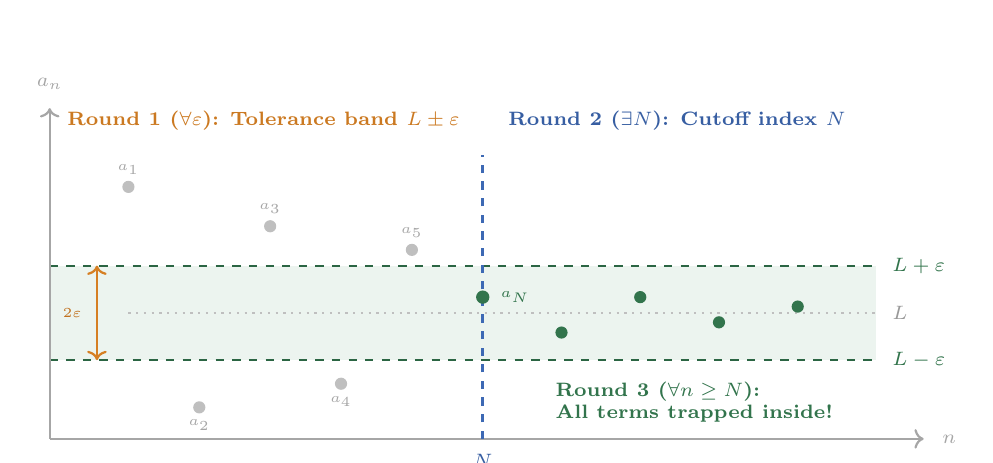
\begin{tikzpicture}[
    font=\small
]

% Epsilon band shading
\fill[targetgreen!10] (0.5, 1.4) rectangle (11.0, 2.6);

% Horizontal band boundaries
\draw[targetgreen!70!black, dashed, thick] (0.5, 2.6) -- (11.0, 2.6) node[right=2pt, font=\scriptsize, text=targetgreen!80!black] {$L + \eps$};
\draw[targetgreen!70!black, dashed, thick] (0.5, 1.4) -- (11.0, 1.4) node[right=2pt, font=\scriptsize, text=targetgreen!80!black] {$L - \eps$};

% Target limit L line
\draw[gray!50, dotted, thick] (1.5, 2.0) -- (11.0, 2.0) node[right=2pt, font=\scriptsize, text=gray!80] {$L$};

% Axes
\draw[->, thick, gray!70] (0.5, 0.4) -- (11.6, 0.4) node[right=3pt, font=\scriptsize] {$n$};
\draw[->, thick, gray!70] (0.5, 0.4) -- (0.5, 4.6) node[above=3pt, font=\scriptsize] {$a_n$};

% Epsilon width indicator
\draw[<->, thick, quotientorange] (1.1, 1.4) -- (1.1, 2.6);
\node[left=2pt, font=\tiny\bfseries, text=quotientorange!90!black] at (1.1, 2.0) {$2\eps$};

% Cutoff N vertical line
\draw[very thick, sourceblue, dashed] (6.0, 0.4) -- (6.0, 4.0);
\node[below=2pt, font=\scriptsize\bfseries, text=sourceblue!90!black] at (6.0, 0.4) {$N$};

% Round 1 callout
\node[anchor=south west, font=\scriptsize\bfseries, text=quotientorange!95!black] at (0.6, 4.2) {Round 1 ($\forall \eps$): Tolerance band $L \pm \eps$};

% Round 2 callout
\node[anchor=south west, font=\scriptsize\bfseries, text=sourceblue!90!black] at (6.2, 4.2) {Round 2 ($\exists N$): Cutoff index $N$};

% Round 3 callout
\node[anchor=north west, font=\scriptsize\bfseries, text=targetgreen!80!black, align=left] at (6.8, 1.25) {Round 3 ($\forall n \ge N$):\\All terms trapped inside!};

% Early terms (outside or wandering)
\fill[gray!50] (1.5, 3.6) circle (2.2pt) node[above=1pt, font=\tiny, text=gray!70] {$a_1$};
\fill[gray!50] (2.4, 0.8) circle (2.2pt) node[below=1pt, font=\tiny, text=gray!70] {$a_2$};
\fill[gray!50] (3.3, 3.1) circle (2.2pt) node[above=1pt, font=\tiny, text=gray!70] {$a_3$};
\fill[gray!50] (4.2, 1.1) circle (2.2pt) node[below=1pt, font=\tiny, text=gray!70] {$a_4$};
\fill[gray!50] (5.1, 2.8) circle (2.2pt) node[above=1pt, font=\tiny, text=gray!70] {$a_5$};

% Terms from N onward (safely trapped)
\fill[targetgreen!80!black] (6.0, 2.2) circle (2.4pt);
\node[right=3pt, font=\tiny\bfseries, text=targetgreen!80!black] at (6.0, 2.2) {$a_N$};
\fill[targetgreen!80!black] (7.0, 1.75) circle (2.2pt);
\fill[targetgreen!80!black] (8.0, 2.20) circle (2.2pt);
\fill[targetgreen!80!black] (9.0, 1.88) circle (2.2pt);
\fill[targetgreen!80!black] (10.0, 2.08) circle (2.2pt);

\end{tikzpicture}
\caption{The three-round quantifier game for the limit of a sequence ($\forall \eps > 0, \exists N \in \N, \forall n \ge N, |a_n - L| < \eps$). In Round~1, the Challenger narrows the tolerance corridor to $L \pm \eps$. In Round~2, the Prover inspects $\eps$ and chooses a cutoff index $N$. In Round~3, the Challenger tests any $n \ge N$: all terms from $N$ onward satisfy the condition $|a_n - L| < \eps$.}
\label{04:fig-limit-game}
\end{figure}

What if a quantified claim is false? How do you mathematically disagree with an assertion containing multiple quantifiers?

If an adversary claims that $\forall x \in D, \, \exists y \in D, \, P(x, y)$, refuting them requires you to step into the shoes of the Challenger. You must establish that \emph{there exists an element $x \in D$} for which \emph{every possible response $y$} fails:
\[
\neg \bigl(\forall x \in D, \, \exists y \in D, \, P(x, y)\bigr) \iff \exists x \in D, \, \forall y \in D, \, \neg P(x, y).
\]
Notice the systematic inversion: every $\forall$ transforms into an $\exists$, every $\exists$ transforms into a $\forall$, and the condition is negated. Negation exchanges the roles of the universal and existential quantifiers.

In Chapter~5 (\emph{Negation: How to Disagree Precisely}), we examine the systematic rules for negating quantified statements and constructing counterexamples.

\subsection{Exercises}

\subsubsection*{Part A: Warm-Up Mental Checks}
State whether each statement is true or false, and justify your answer in a single sentence:
\begin{enumerate}
\item $\forall x \in \R, \, \exists y \in \R \text{ such that } x + y = 10$.
\item $\exists y \in \R \text{ such that } \forall x \in \R, \, x + y = 10$.
\item $\forall x \in \Z, \, \exists y \in \Z \text{ such that } x - y \text{ is an even integer}$.
\end{enumerate}

\subsubsection*{Part B: Routine Game Practice}
Determine whether each statement is true or false. Provide a winning strategy for the Prover, or an adversary's winning counter-move:
\begin{enumerate}[resume]
\item $\forall x \in \R, \, \exists y \in \R \text{ such that } x < y$.
\item $\exists y \in \R \text{ such that } \forall x \in \R, \, x < y$.
\item $\forall x \in \R, \, \exists y \in \R \text{ such that } xy = 1$.
\item $\forall x \in (\R \setminus \{0\}), \, \exists y \in \R \text{ such that } xy = 1$.
\item $\exists y \in \R \text{ such that } \forall x \in \R, \, xy = 0$.
\item $\forall x \in \N, \, \exists y \in \N \text{ such that } y < x$ (where $\N = \{1, 2, 3, \ldots\}$).
\end{enumerate}

\subsubsection*{Part C: Proof Skeletons}
For each claim below, write only the opening declaration (introducing variables and their roles) and the final verification line of a direct proof. Do not carry out the calculations:
\begin{enumerate}[resume]
\item $\forall x \in \R, \, \exists y \in \R \text{ such that } y^3 = x$.
\item $\exists c \in \R \text{ such that } \forall x \in \R, \, x^2 + c \ge 0$.
\end{enumerate}

\subsubsection*{Part D: Deeper Challenges}
\begin{enumerate}[resume]
\item Write out a rigorous four-step proof that for any non-empty domain $D$ and any predicate $P(x, y)$, the implication $\bigl(\exists y \in D \, \forall x \in D \, P(x, y)\bigr) \implies \bigl(\forall x \in D \, \exists y \in D \, P(x, y)\bigr)$ is valid. Explicitly state the role (arbitrary vs.\ chosen) of each variable you introduce.
\item Consider the three-quantifier sentence on the real numbers:
\[
\forall x \in \R, \, \exists y \in \R, \, \forall z \in \R, \, x + y + z > 0.
\]
Is this statement true or false? Play the three-round game step by step to prove your conclusion.
\end{enumerate}

\begin{walkbox}
Think of the definition of the limit of a sequence: ``For every $\eps > 0$, there exists an index $N$ such that\ldots'' Who moves first in this game? Does $N$ depend on $\eps$, or does $\eps$ depend on $N$? What would it mean if the quantifiers were reversed: ``There exists an index $N$ such that for every $\eps > 0$\ldots''? Could any sequence except an eventually constant one satisfy that reversed condition?
\end{walkbox}

\newpage

\section{Negation: How to Disagree Precisely}
\chapterline

In ordinary conversation, disagreement can be vague. If someone declares ``Everyone loves summer,'' an everyday response might be ``I don't!'' or ``That's not true, winter is great.'' The everyday meaning is easily understood, but English allows ambiguity to creep in: does ``everyone doesn't love summer'' mean nobody loves it, or merely that at least one person does not?

In mathematics, negation is not an attitude or a rhetorical rebuttal. It is a razor-sharp logical operation. To negate a statement $P$ means to construct the exact statement $\neg P$ that is true when $P$ is false, and false when $P$ is true. 

If you cannot state the exact negation of a theorem or definition, you cannot construct a proof by contradiction, and you cannot recognize when a proposed counterexample actually refutes a claim.

\begin{historybox}
In the 1910s and 1920s, the Dutch topologist L.E.J. Brouwer triggered one of the most intense civil wars in modern mathematics by questioning the meaning of negation on infinite collections. In classical logic, every statement is assumed to be either true or false (the Law of the Excluded Middle, $P \lor \neg P$). Under this rule, proving that a statement cannot be false automatically proves that it is true ($\neg \neg P \implies P$).

Brouwer pointed out a subtle dilemma: on a finite list of numbers, checking whether a property holds is straightforward; if no counterexample exists, you eventually inspect every number and know it is true. But on an infinite set, showing that ``it is impossible for no solution to exist'' does not hand you the solution! Brouwer argued that unless you can build the object in a finite number of steps, claiming it exists through double negation is an empty illusion. 

David Hilbert defended classical logic with fierce intensity. To Hilbert, banning indirect negation was like ``forbidding the telescope to the astronomer or the use of his fists to the boxer.'' Hilbert famously declared: ``No one shall expel us from the paradise that Cantor created.'' Hermann Weyl, one of Hilbert's greatest students, briefly joined Brouwer, warning that classical analysis was a house built on sand, before modern logic demonstrated that both constructive and classical systems could coexist with distinct virtues. In classical proof writing, mastering exact negation remains our most reliable weapon for exposing logical gaps and formulating counterexamples.
\end{historybox}

\subsection{Negating quantifiers: crossing the boundary}

The central rule of quantifier negation is that \textbf{negation swaps the quantifier and moves inside}:
\begin{align*}
\neg \bigl(\forall x \in D, \, P(x)\bigr) &\iff \exists x \in D \text{ such that } \neg P(x), \\
\neg \bigl(\exists x \in D \text{ such that } P(x)\bigr) &\iff \forall x \in D, \, \neg P(x).
\end{align*}

Why does this flip occur? Think of the universe of discourse $D$ geometrically. Let $S = \{x \in D : P(x)\}$ be the territory where property $P$ holds, and let its complement $S^c = \{x \in D : \neg P(x)\}$ be the territory where property $P$ fails.

\begin{center}
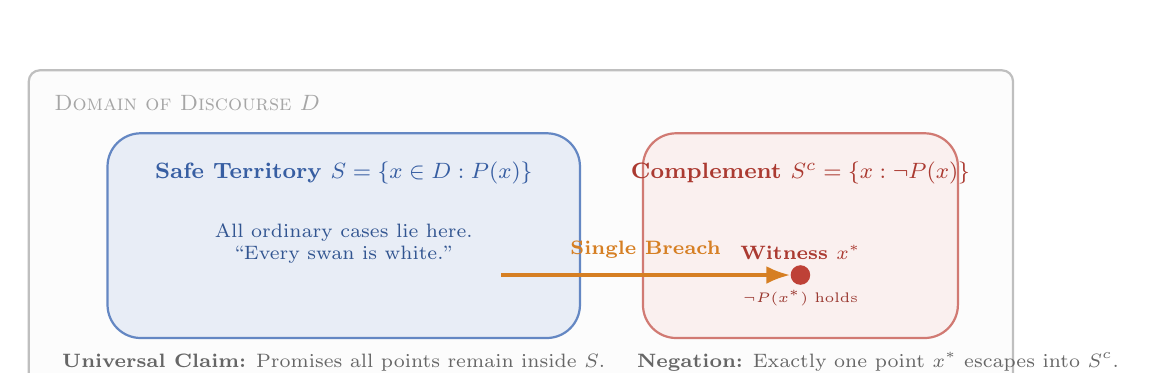
\begin{tikzpicture}[
    font=\small,
    universe/.style={draw=gray!50, fill=gray!2, rounded corners=4pt, thick},
    claimset/.style={draw=sourceblue!80, fill=sourceblue!12, rounded corners=12pt, thick},
    badset/.style={draw=trapred!70, fill=trapred!8, rounded corners=12pt, thick}
]

% Universe Box
\draw[universe] (0, 0) rectangle (12.5, 4.0);
\node[anchor=north west, font=\footnotesize\scshape, text=gray!70] at (0.2, 3.8) {Domain of Discourse $D$};

% Satisfying Region S
\draw[claimset] (1.0, 0.6) rectangle (7.0, 3.2);
\node[font=\footnotesize\bfseries, text=sourceblue!90!black] at (4.0, 2.7) {Safe Territory $S = \{x \in D : P(x)\}$};
\node[font=\scriptsize, text=sourceblue!80!black, align=center] at (4.0, 1.8) {All ordinary cases lie here.\\``Every swan is white.''};

% Complement Region S^c
\draw[badset] (7.8, 0.6) rectangle (11.8, 3.2);
\node[font=\footnotesize\bfseries, text=trapred!90!black] at (9.8, 2.7) {Complement $S^c = \{x : \neg P(x)\}$};

% The Escaped Witness
\node[circle, fill=trapred, inner sep=2.5pt] (witness) at (9.8, 1.4) {};
\node[above=2pt, font=\scriptsize\bfseries, text=trapred!90!black] at (witness) {Witness $x^*$};
\node[below=2pt, font=\tiny, text=trapred!80!black] at (witness) {$\neg P(x^*)$ holds};

% Boundary crossing arrow
\draw[-{Latex[length=3mm]}, very thick, quotientorange] (6.0, 1.4) -- node[above=2pt, font=\scriptsize\bfseries, text=quotientorange]{Single Breach} (witness);

% Bottom summary note
\node[anchor=west, font=\scriptsize, text=gray!80!black] at (0.3, 0.3) {
    \textbf{Universal Claim:} Promises all points remain inside $S$. \quad
    \textbf{Negation:} Exactly one point $x^*$ escapes into $S^c$.
};

\end{tikzpicture}
\end{center}

A universal claim asserts that \emph{every} point in the domain remains strictly inside the safe territory $S$. To tear that claim down, you do not need every point to escape. You do not need the entire world to fail. You need only a single witness $x^*$ that crosses the boundary into $S^c$.

Conversely, an existential claim asserts that at least one point lives in $S$. To refute that claim, you cannot simply show that some point misses. You must demonstrate that \emph{every} point in $D$ fails to enter $S$.

\subsection{Negating implications: the broken contract}

Beginners frequently stumble when negating an if-then statement. When asked to negate:
\begin{quote}
``If it rains, then the ground is wet'' ($P \implies Q$),
\end{quote}
an intuitive first guess is often ``If it rains, then the ground is dry.'' But that is not a negation; that is a brand new, aggressive implication.

An implication $P \implies Q$ is a contractual guarantee:
\begin{center}
\itshape ``Whenever condition $P$ is fulfilled, I promise outcome $Q$ will occur.''
\end{center}
Under what exact circumstance is this contract broken? 
\begin{itemize}
\item If it does not rain, the contract was never tested. No promise has been broken.
\item If it rains and the ground is wet, the contract was honored.
\item The contract is broken \textbf{if and only if} it rains, and yet the ground remains dry.
\end{itemize}

Therefore, the negation of an implication is never an if-then statement. It is a conjunction:
\[
\neg(P \implies Q) \iff P \land \neg Q.
\]
To disprove $P \implies Q$, you must produce an instance where the hypothesis $P$ is fully satisfied, while the conclusion $Q$ fails.

\subsection{De Morgan's laws: the duality of AND and OR}

When negating composite conditions involving ``and'' ($\land$) or ``or'' ($\lor$), Augustus De Morgan observed a fundamental duality:
\begin{align*}
\neg(P \land Q) &\iff \neg P \lor \neg Q, \\
\neg(P \lor Q) &\iff \neg P \land \neg Q.
\end{align*}

\begin{center}
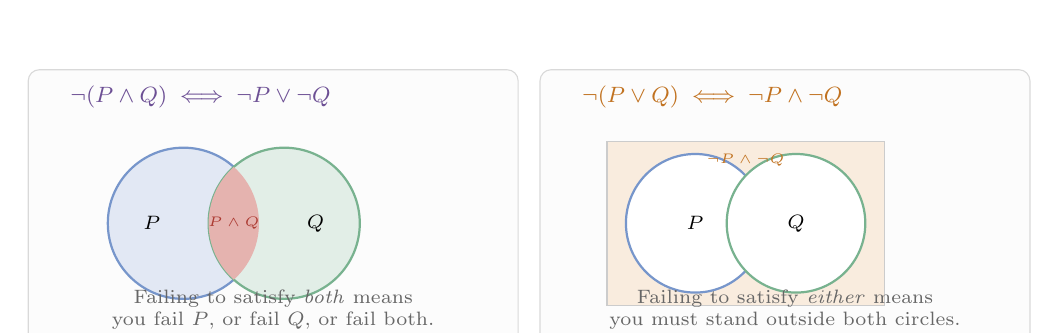
\begin{tikzpicture}[
    font=\small,
    subpanel/.style={draw=gray!30, fill=gray!2, rounded corners=4pt, inner sep=6pt}
]

% Panel A: Negation of AND
\node[subpanel, text width=5.8cm, minimum height=3.5cm] (p1) at (0, 0) {};
\node[anchor=west, font=\footnotesize\scshape, text=structurepurple!90!black] at (-2.7, 1.4) {$\neg(P \land Q) \iff \neg P \lor \neg Q$};

\begin{scope}[xshift=-0.5cm, yshift=-0.2cm, scale=0.8]
    % Circles
    \draw[thick, draw=sourceblue!70, fill=sourceblue!15] (-0.8, 0) circle (1.2);
    \draw[thick, draw=targetgreen!70, fill=targetgreen!15] (0.8, 0) circle (1.2);
    
    % Lens (P and Q)
    \begin{scope}
        \clip (-0.8, 0) circle (1.2);
        \fill[trapred!40] (0.8, 0) circle (1.2);
    \end{scope}
    
    \node[font=\scriptsize] at (-1.3, 0) {$P$};
    \node[font=\scriptsize] at (1.3, 0) {$Q$};
    \node[font=\tiny\bfseries, text=trapred!90!black] at (0, 0) {$P \land Q$};
\end{scope}

\node[font=\scriptsize, text=gray!80!black, align=center] at (0, -1.3) {
    Failing to satisfy \emph{both} means\\you fail $P$, or fail $Q$, or fail both.
};

% Panel B: Negation of OR
\node[subpanel, text width=5.8cm, minimum height=3.5cm] (p2) at (6.5, 0) {};
\node[anchor=west, font=\footnotesize\scshape, text=quotientorange!90!black] at (3.8, 1.4) {$\neg(P \lor Q) \iff \neg P \land \neg Q$};

\begin{scope}[xshift=6.0cm, yshift=-0.2cm, scale=0.8]
    % Surrounding universe shaded
    \draw[fill=quotientorange!15, draw=gray!40] (-2.2, -1.3) rectangle (2.2, 1.3);
    
    % Both circles unshaded / white
    \draw[thick, draw=sourceblue!70, fill=white] (-0.8, 0) circle (1.1);
    \draw[thick, draw=targetgreen!70, fill=white] (0.8, 0) circle (1.1);
    
    \node[font=\scriptsize] at (-0.8, 0) {$P$};
    \node[font=\scriptsize] at (0.8, 0) {$Q$};
    \node[font=\tiny\bfseries, text=quotientorange!90!black] at (0, 1.0) {$\neg P \land \neg Q$};
\end{scope}

\node[font=\scriptsize, text=gray!80!black, align=center] at (6.5, -1.3) {
    Failing to satisfy \emph{either} means\\you must stand outside both circles.
};

\end{tikzpicture}
\end{center}

If a club requires you to be ``over 21 \textbf{and} a resident of California,'' what does it take to be denied entry? You do not need to fail both requirements. You are denied if you are under 21, \textbf{or} if you are not a resident of California.

\subsection{Negating a multi-quantifier statement: step-by-step}

Let us negate the formal definition of sequence convergence. The statement $a_n \to L$ as $n \to \infty$ means:
\[
\forall \eps > 0, \, \exists N \in \N, \, \forall n \ge N, \, |a_n - L| < \eps.
\]

To negate this, we push the negation symbol through the quantifiers one by one from left to right:
\begin{align*}
\neg \bigl(\forall \eps > 0, \ldots\bigr) &\iff \exists \eps > 0 \text{ such that } \neg \bigl(\exists N \in \N, \ldots\bigr) \\
&\iff \exists \eps > 0, \, \forall N \in \N, \, \neg \bigl(\forall n \ge N, \ldots\bigr) \\
&\iff \exists \eps > 0, \, \forall N \in \N, \, \exists n \ge N \text{ such that } |a_n - L| \ge \eps.
\end{align*}

Read this final line in plain English: there is some tolerance band of radius $\eps > 0$ such that no matter how far out you travel into the sequence (for every index $N$), you can always find a later term $n \ge N$ that escapes the band. The sequence never settles down inside the $\eps$-tube.

\subsection{What precise negation unlocked---and the need for definition machines}

The algebraic calculus of negation transformed disagreement from a rhetorical clash of opinions into a mechanical procedure. By pushing negations through quantifier prefixes ($\neg \forall \to \exists \neg$) and breaking down conditional contracts ($\neg(P \implies Q) \iff P \land \neg Q$), mathematicians gained an exact recipe for refutation: to shatter a universal promise, you do not need to tear down the entire world; you need only construct a single witness that satisfies the premise while violating the conclusion.

Yet knowing how to manipulate symbols like $\neg, \forall,$ and $\implies$ hits a brick wall if the words inside the sentences remain hazy. If someone claims that ``every continuous function is differentiable'', formal negation tells you to find a function that is continuous but not differentiable. But what do the words ``continuous'' and ``differentiable'' actually demand under the hood? If mathematical vocabulary is treated like a dictionary definition with poetic flexibility, you can never prove whether a candidate witness genuinely qualifies. 

In Chapter~6 (\emph{Definitions: The Machines Inside the Words}), we open up mathematical terms, discovering that definitions in pure mathematics are not summaries of usage, but rigid two-way algebraic sorting machines.

\subsection{Exercises}

Negate each statement completely, so that no negation symbol appears outside a quantifier or connective:
\begin{enumerate}
\item Every real number has a real cube root: $\forall x \in \R, \, \exists y \in \R, \, y^3 = x$.
\item There is an integer whose square is negative: $\exists n \in \Z, \, n^2 < 0$.
\item For every $x > 0$, there exists $y > 0$ such that $xy = 1$.
\item If $n$ is prime, then $n = 2$ or $n$ is odd.
\item $\forall x \in A, \, \bigl(P(x) \implies \exists y \in B, \, Q(x, y)\bigr)$.
\item The function $f : \R \to \R$ is bounded: $\exists M > 0, \, \forall x \in \R, \, |f(x)| \le M$.
\end{enumerate}

\begin{walkbox}
Whenever you read a news headline asserting that ``Nobody wants to do X anymore,'' practice formulating the minimal mathematical negation. Does it require an enthusiastic crowd, or merely one person?
\end{walkbox}

\newpage

\section{Definitions: The Machines Inside the Words}
\chapterline

In Chapter~5, we treated mathematical claims as geometric territories: a universal statement promises that every object stays inside a safe region, and negating it means hunting for a single witness that steps outside. But this raises an essential question: what draws the boundary line in the first place? How do we determine whether a candidate number, function, or geometric shape belongs inside the territory or stands outside it?

In everyday language, definitions are largely descriptive. Dictionaries record how words are commonly used, capturing nuances, historical context, and loose associations. If someone asks what makes a cup a ``mug,'' one might mention a handle, a cylindrical ceramic shape, and its use for hot drinks. If a container lacks a handle or is made of glass, whether it counts as a mug remains open to informal debate. Everyday language tolerates imprecise boundaries.

In pure mathematics, a definition is not a descriptive summary; it is an exact specification. It establishes precise criteria that classify mathematical objects unambiguously. Every object either satisfies all stated conditions and belongs to the defined category, or fails at least one condition and does not.

\begin{figure}[htbp]
\centering
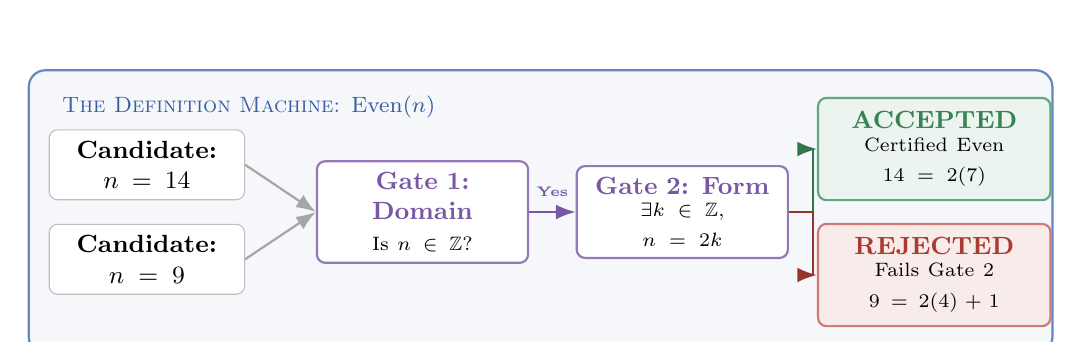
\begin{tikzpicture}[
    font=\small,
    machine/.style={draw=sourceblue!80, fill=sourceblue!5, rounded corners=6pt, thick, inner sep=10pt},
    gate/.style={draw=structurepurple!80, fill=white, rounded corners=3pt, thick, text width=2.4cm, align=center, inner sep=4pt},
    inout/.style={draw=gray!50, fill=white, rounded corners=3pt, text width=2.2cm, align=center, inner sep=4pt}
]

% Main machine boundary
\node[machine, minimum width=13.0cm, minimum height=3.6cm] (box) at (6.0, 0) {};
\node[anchor=north west, font=\footnotesize\scshape, text=sourceblue!90!black] at (-0.2, 1.6) {The Definition Machine: $\operatorname{Even}(n)$};

% Left: Candidate Inputs
\node[inout] (in1) at (1.0, 0.6) {\textbf{Candidate:} $n = 14$};
\node[inout] (in2) at (1.0, -0.6) {\textbf{Candidate:} $n = 9$};

% Gates inside machine
\node[gate] (g1) at (4.5, 0) {\textbf{\color{structurepurple}Gate 1: Domain}\\\scriptsize Is $n \in \Z$?};
\node[gate] (g2) at (7.8, 0) {\textbf{\color{structurepurple}Gate 2: Form}\\\scriptsize $\exists k \in \Z,$\\$n = 2k$};

% Output streams
\node[draw=targetgreen!80, fill=targetgreen!10, rounded corners=3pt, thick, text width=2.6cm, align=center, inner sep=5pt] (outT) at (11.0, 0.8) {
    \textbf{\color{targetgreen!90!black}ACCEPTED}\\\scriptsize Certified Even\\$14 = 2(7)$
};

\node[draw=trapred!70, fill=trapred!10, rounded corners=3pt, thick, text width=2.6cm, align=center, inner sep=5pt] (outF) at (11.0, -0.8) {
    \textbf{\color{trapred!90!black}REJECTED}\\\scriptsize Fails Gate 2\\$9 = 2(4) + 1$
};

% Connecting arrows
\draw[-{Latex[length=2.5mm]}, thick, gray!70] (in1.east) -- (g1.west);
\draw[-{Latex[length=2.5mm]}, thick, gray!70] (in2.east) -- (g1.west);

\draw[-{Latex[length=2.5mm]}, thick, structurepurple] (g1) -- node[above=2pt, font=\tiny\bfseries, text=structurepurple]{Yes} (g2);

\draw[-{Latex[length=2.5mm]}, thick, targetgreen!80!black] (g2.east) -- ++(0.3, 0) |- (outT.west);
\draw[-{Latex[length=2.5mm]}, thick, trapred!80!black] (g2.east) -- ++(0.3, 0) |- (outF.west);

\end{tikzpicture}
\caption{A mathematical definition viewed as a two-stage condition check. Candidate objects arrive from the left and must pass each requirement. Candidate $n = 14$ is an integer (Gate 1) and factors as $2 \times 7$ (Gate 2), so it satisfies both conditions and is classified as even. Candidate $n = 9$ is an integer but fails the factorization test, so it is not even.}
\label{06:fig-definition-machine-even}
\end{figure}

\begin{historybox}
Throughout the eighteenth century, calculus pioneers including Leonhard Euler and Joseph-Louis Lagrange treated definitions as descriptive summaries of geometric intuition. A \emph{continuous curve} was described informally as a line drawn across paper without lifting the quill, and mathematicians took for granted that any unbroken curve must possess a well-defined tangent line---an instantaneous slope or derivative---at almost every point. If you could sketch it without tears or leaps, smooth calculus tools were assumed to apply.

In 1872, Karl Weierstrass challenged this visual confidence by introducing a counterexample to the Berlin Academy: an infinite sum of cosine oscillations, adding infinitely many ripple waves of ever-smaller wavelengths and ever-steeper slopes. The resulting curve has no breaks or gaps, yet it is nowhere differentiable. At every single point, under every level of magnification, the curve consists entirely of sharp corners, never flattening into a line. Charles Hermite recoiled with ``fright and horror from this lamentable plague of functions without derivatives,'' while Henri Poincar\'e complained that logic had invented monsters to mock common sense.

Yet Bernard Bolzano (in 1817) and Weierstrass realized that the fault lay not in the functions, but in relying on human sketches. An ink line on paper has physical thickness that hides microscopic oscillations. Definitions could no longer be fuzzy summaries of visual intuition; they had to become rigid sorting machines governed by quantifiers ($\forall$ and $\exists$) and exact inequality contracts ($\eps$ and $\delta$). By defining continuity through arithmetic bounds rather than sketches, mathematics grounded proof in symbolic precision.

This shift remains vital today: in modern computer proof assistants such as Lean, Coq, and Isabelle, mathematical definitions are literally encoded as machine-checked sorting gates. A major frontier in modern mathematical reasoning is whether automated systems can learn to formulate the right minimal definitions on their own, rather than merely verifying human-crafted ones.
\end{historybox}

\subsection{The two operations: unpacking and packaging}

Every mathematical definition operates as a bidirectional pipeline. Depending on where you stand in a proof, you will use it in one of two modes:

\begin{enumerate}
\item \textbf{Unpacking (Using the Definition)}: You are \emph{given} that an object satisfies a definition. 
The definition allows you to replace the term with its explicit mathematical conditions:
\begin{quote}
``Since $n$ is even, there exists some integer $k$ such that $n = 2k$.''
\end{quote}
Here, the word ``even'' is replaced by a concrete algebraic equation ($n = 2k$) that you can substitute, manipulate, or factor.

\item \textbf{Packaging (Applying the Definition)}: You have performed algebraic manipulations and want to \emph{conclude} that an object satisfies a definition.
The definition specifies the exact entrance criteria you must satisfy:
\begin{quote}
``Since $m = 2(j^2 + j)$ where $j^2 + j \in \Z$, the number $m$ is of the form $2k$ for an integer $k$. Therefore, $m$ is even.''
\end{quote}
Here, you verify that the expression satisfies the conditions and conclude that $m$ is even.
\end{enumerate}

Early proof writing is largely the discipline of alternating cleanly between unpacking your hypotheses and packaging your conclusions, as illustrated in Figure~\ref{06:fig-unpack-package-pipeline}.

\begin{figure}[htbp]
\centering
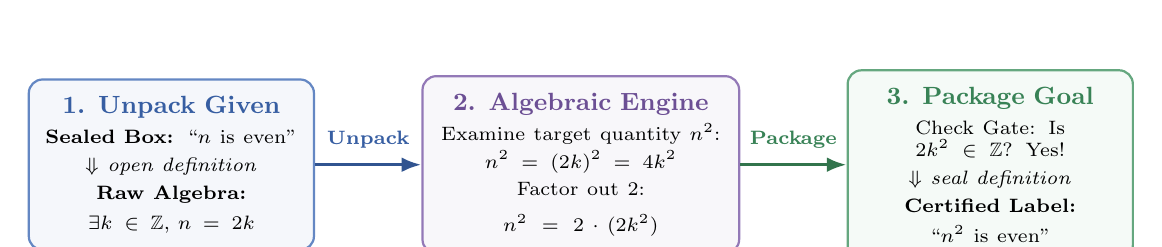
\begin{tikzpicture}[
    font=\small,
    stage/.style={draw=gray!60, fill=white, rounded corners=5pt, thick, inner sep=6pt, text width=3.2cm, align=center},
    steparrow/.style={-{Latex[length=2.5mm]}, very thick}
]

% Stage 1: Unpack
\node[stage, draw=sourceblue!80, fill=sourceblue!5] (s1) at (1.6, 0) {
    \textbf{\color{sourceblue!90!black}1. Unpack Given}\\[3pt]
    \scriptsize \textbf{Sealed Box:} ``$n$ is even''\\[2pt]
    $\Downarrow$ \emph{open definition}\\[2pt]
    \textbf{Raw Algebra:}\\
    $\exists k \in \Z, \, n = 2k$
};

% Stage 2: Algebraic Manipulation
\node[stage, draw=structurepurple!80, fill=structurepurple!5, text width=3.6cm] (s2) at (6.8, 0) {
    \textbf{\color{structurepurple!90!black}2. Algebraic Engine}\\[3pt]
    \scriptsize Examine target quantity $n^2$:\\[2pt]
    $n^2 = (2k)^2 = 4k^2$\\[2pt]
    Factor out $2$:\\[2pt]
    $n^2 = 2 \cdot (2k^2)$
};

% Stage 3: Package
\node[stage, draw=targetgreen!80, fill=targetgreen!5] (s3) at (12.0, 0) {
    \textbf{\color{targetgreen!90!black}3. Package Goal}\\[3pt]
    \scriptsize Check Gate: Is $2k^2 \in \Z$? Yes!\\[2pt]
    $\Downarrow$ \emph{seal definition}\\[2pt]
    \textbf{Certified Label:}\\
    ``$n^2$ is even''
};

% Connecting Arrows
\draw[steparrow, sourceblue!80!black] (s1.east) -- node[above=2pt, font=\scriptsize\bfseries, text=sourceblue!90!black]{Unpack} (s2.west);
\draw[steparrow, targetgreen!80!black] (s2.east) -- node[above=2pt, font=\scriptsize\bfseries, text=targetgreen!90!black]{Package} (s3.west);

\end{tikzpicture}
\caption{Unpacking and packaging in a direct proof. On the left, we unpack the hypothesis: replacing the term ``even'' with the algebraic statement $n = 2k$ for some $k \in \Z$. In the center, we manipulate the expression algebraically into the form $2 \cdot (\text{integer})$. On the right, we verify that the condition is met and conclude that $n^2$ is even.}
\label{06:fig-unpack-package-pipeline}
\end{figure}

\subsection{Divisibility: a definition to handle with care}

Let us inspect a standard arithmetic definition that beginners often mangle:

\begin{definition}
Let $a, b \in \Z$. We say that $a$ \emph{divides} $b$, written $a \mid b$, if there exists an integer $k$ such that $b = ak$.
\end{definition}

In plain language, $a \mid b$ means that $b$ is an exact whole-number multiple of $a$. Imagine a measuring rod of length $a$: it can tile a segment of length $b$ perfectly, with no leftover remainder.

Notice the orientation of the symbols:
\begin{itemize}
\item $3 \mid 12$ is true because $12 = 3(4)$. Here $a = 3$, $b = 12$, and the witness integer is $k = 4$.
\item $12 \mid 3$ is false because there is no integer $k$ satisfying $3 = 12k$ (the only real solution is $k = 1/4$, which fails the integer gate requirement).
\end{itemize}

Figure~\ref{06:fig-divisibility-tiling} illustrates this measuring-rod model: $a$ divides $b$ precisely when rods of length $a$ tile the interval $[0, b]$ without gap or overlap.

\begin{figure}[htbp]
\centering
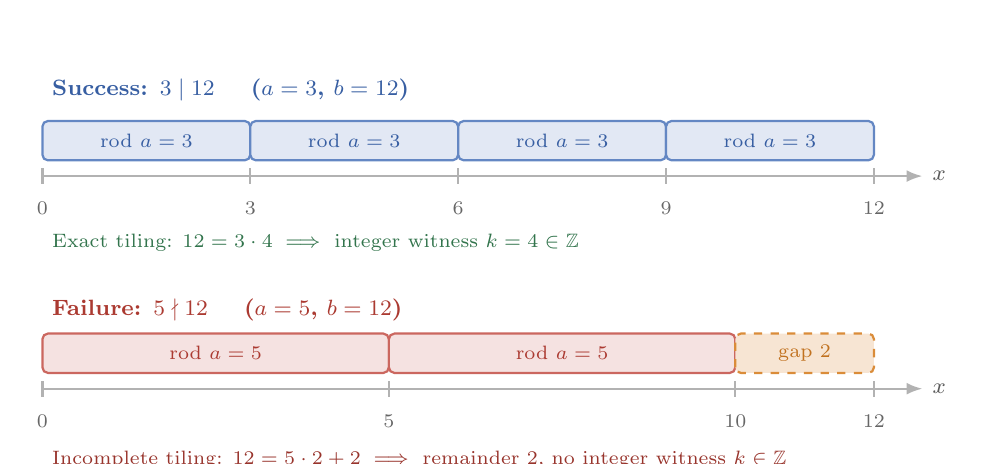
\begin{tikzpicture}[
    x=0.88cm, y=1cm,
    font=\small,
    rod/.style={draw=sourceblue!80, fill=sourceblue!15, rounded corners=2pt, thick, inner sep=0pt},
    failrod/.style={draw=trapred!80, fill=trapred!15, rounded corners=2pt, thick, inner sep=0pt},
    remrod/.style={draw=quotientorange!90, fill=quotientorange!20, dashed, rounded corners=2pt, thick, inner sep=0pt},
    axis/.style={-{Latex[length=2mm]}, thick, gray!60}
]

% Top case: 3 | 12
\node[anchor=west, font=\footnotesize\bfseries, text=sourceblue!90!black] at (0, 3.1) {Success: $3 \mid 12$ \quad ($a = 3$, $b = 12$)};
\draw[axis] (0, 2.0) -- (12.7, 2.0) node[right, font=\footnotesize, text=gray!70!black] {$x$};
\foreach \x in {0, 3, 6, 9, 12} {
    \draw[gray!60, thick] (\x, 1.9) -- (\x, 2.1);
    \node[below=3pt, font=\scriptsize, text=gray!80!black] at (\x, 1.9) {$\x$};
}
\draw[rod] (0, 2.2) rectangle ++(3, 0.5) node[pos=0.5, font=\scriptsize, text=sourceblue!90!black]{rod $a=3$};
\draw[rod] (3, 2.2) rectangle ++(3, 0.5) node[pos=0.5, font=\scriptsize, text=sourceblue!90!black]{rod $a=3$};
\draw[rod] (6, 2.2) rectangle ++(3, 0.5) node[pos=0.5, font=\scriptsize, text=sourceblue!90!black]{rod $a=3$};
\draw[rod] (9, 2.2) rectangle ++(3, 0.5) node[pos=0.5, font=\scriptsize, text=sourceblue!90!black]{rod $a=3$};
\node[anchor=west, font=\scriptsize, text=targetgreen!80!black] at (0, 1.15) {Exact tiling: $12 = 3 \cdot 4 \implies$ integer witness $k = 4 \in \Z$};

% Bottom case: 5 does not divide 12
\node[anchor=west, font=\footnotesize\bfseries, text=trapred!90!black] at (0, 0.3) {Failure: $5 \nmid 12$ \quad ($a = 5$, $b = 12$)};
\draw[axis] (0, -0.7) -- (12.7, -0.7) node[right, font=\footnotesize, text=gray!70!black] {$x$};
\foreach \x in {0, 5, 10, 12} {
    \draw[gray!60, thick] (\x, -0.8) -- (\x, -0.6);
    \node[below=3pt, font=\scriptsize, text=gray!80!black] at (\x, -0.8) {$\x$};
}
\draw[failrod] (0, -0.5) rectangle ++(5, 0.5) node[pos=0.5, font=\scriptsize, text=trapred!90!black]{rod $a=5$};
\draw[failrod] (5, -0.5) rectangle ++(5, 0.5) node[pos=0.5, font=\scriptsize, text=trapred!90!black]{rod $a=5$};
\draw[remrod] (10, -0.5) rectangle ++(2, 0.5) node[pos=0.5, font=\scriptsize, text=quotientorange!90!black]{gap $2$};
\node[anchor=west, font=\scriptsize, text=trapred!80!black] at (0, -1.6) {Incomplete tiling: $12 = 5 \cdot 2 + 2 \implies$ remainder $2$, no integer witness $k \in \Z$};

\end{tikzpicture}
\caption{The integer tiling interpretation of divisibility $a \mid b$. In the upper case, the interval $[0, 12]$ is tiled exactly by four rods of length $a = 3$, certifying that $3 \mid 12$ with integer witness $k = 4$. In the lower case, attempting to tile $[0, 12]$ with rods of length $a = 5$ leaves an incomplete gap of length $2$, so no integer multiplier exists and $5 \nmid 12$.}
\label{06:fig-divisibility-tiling}
\end{figure}

\begin{trapbox}
Do not confuse the vertical bar $a \mid b$ with the forward slash $a / b$.
\begin{itemize}
\item $a \mid b$ is a \textbf{statement} (an assertion that can be true or false).
\item $a / b$ is a \textbf{term} (an algebraic expression denoting a rational number).
\end{itemize}
Writing ``if $a / b$ then\ldots'' is a grammatical type error: you cannot place a numerical quantity into the condition slot of an if-then statement.
\end{trapbox}

Beginners often stumble on boundary cases involving zero and negative numbers because intuition confuses the relational statement $a \mid b$ with the algorithmic process of long division:
\begin{itemize}
\item \textbf{Does $3 \mid 0$?} Run it through the machine: does there exist an integer $k$ such that $0 = 3k$? Setting $k = 0$ works, since $0 = 3(0)$. Thus, $3 \mid 0$ is true! In fact, every integer $a$ divides $0$, because $0 = a \cdot 0$.
\item \textbf{Does $0 \mid 3$?} The machine asks: does there exist an integer $k$ such that $3 = 0 \cdot k$? Since $0 \cdot k = 0$ for every integer $k$, no such witness can ever exist. The machine firmly rejects it: $0 \nmid 3$.
\item \textbf{Negative divisors:} Does $-4 \mid 12$? Yes, because $12 = (-4)(-3)$, and $-3 \in \Z$. Signs are no obstacle for the divisibility machine.
\end{itemize}

\begin{recoverybox}
\textbf{Pause and think}: Before reading further, test these three candidate pairs mentally against the definition of divisibility:
(1) Does $6 \mid 24$? \quad (2) Does $24 \mid 6$? \quad (3) Does $0 \mid 0$?

\emph{Answers}: (1) True: $24 = 6(4)$. (2) False: $6 = 24k$ has no integer solution. (3) True under the formal definition: $0 = 0 \cdot k$ holds for any integer $k$ (for instance, $k = 1$). Note that while $0 \mid 0$ is a valid true relation, the fraction $0/0$ is undefined arithmetic.
\end{recoverybox}

\subsection{Why mathematicians demand minimal, non-redundant criteria}

Why are definitions designed the way they are? Consider how you might describe a square in everyday speech:
\begin{quote}
``A four-sided polygon with equal sides, four right angles, opposite sides parallel, and equal-length perpendicular diagonals that bisect each other.''
\end{quote}
That description is accurate, but redundant as a mathematical definition.

If every consequence were included in the definition of a square, proving that a shape is a square would require verifying every item on that list.

Mathematicians prefer \textbf{minimal, non-redundant definitions}:
\begin{definition}
A \emph{square} is a quadrilateral with four equal sides and one right angle.
\end{definition}
The remaining geometric properties---such as parallel opposite sides, three additional right angles, and perpendicular diagonals that bisect each other---are not part of the definition. They are \emph{theorems} deduced from this minimal set of conditions.

Keeping definitions minimal simplifies proofs:
\begin{itemize}
\item \textbf{Minimal Verification}: To prove an object qualifies, you need only verify the essential defining conditions.
\item \textbf{Deductive Utility}: Once established, all known theorems about that class of objects apply immediately.
\end{itemize}

\begin{trapbox}
\textbf{The Variable Collision Trap}: When a proof provides multiple hypotheses, you must open each box with a \emph{fresh variable name}. 

Suppose you are given that $a \mid b$ and $b \mid c$. A frequent beginner mistake is to write:
\begin{center}
``$b = ak$ and $c = bk$.'' \quad \textbf{(WRONG!)}
\end{center}
By reusing the letter $k$, you have accidentally claimed that the two multipliers are identical: $b/a = c/b$. For instance, $2 \mid 6$ (where the factor is $3$) and $6 \mid 24$ (where the factor is $4$). Reusing $k$ forces $3 = 4$, collapsing your proof into nonsense.

\textbf{Golden Rule}: Every time you unpack an existential definition ($\exists$), introduce a new, unused variable ($j, m, k_1, k_2$).
\end{trapbox}

\subsection{Worked proof: divisibility is transitive}

A relation is \emph{transitive} if it passes along chains: whenever $a$ relates to $b$, and $b$ relates to $c$, then $a$ relates directly to $c$ (like falling dominoes, or ancestral descent: if you are the child of your parent, and your parent is the child of your grandparent, you are the descendant of your grandparent).

Let us watch the unpacking and packaging pipeline in action on a complete, formal proof.

\begin{theorem}\label{06:thm-divisibility-transitive}
Let $a, b, c \in \Z$. If $a \mid b$ and $b \mid c$, then $a \mid c$.
\end{theorem}

\begin{proof}
Suppose $a \mid b$ and $b \mid c$. 

\emph{(Unpacking step)}: By the definition of divisibility applied to $a \mid b$, there exists an integer $j$ such that $b = aj$. Similarly, by definition applied to $b \mid c$, there exists an integer $m$ such that $c = bm$. Notice that we deliberately selected distinct variables $j$ and $m$ to avoid the Variable Collision Trap.

\emph{(Algebraic core)}: We want to show that $c$ is an integer multiple of $a$. Substituting the expression for $b$ into the equation for $c$, we have:
\[
c = bm = (aj)m = a(jm)
\]
by the associative property of integer multiplication. 

\emph{(Packaging step)}: Since $j$ and $m$ are integers, their product $k = jm$ is also an integer (the integers are closed under multiplication). Thus, we have expressed $c$ in the form $c = ak$ for some $k \in \Z$. By definition of divisibility, this means $a \mid c$.
\end{proof}

Every step is accounted for: we opened the definitions to reveal the algebra, manipulated the symbols lawfully, and closed the definition to reach our destination.

Figure~\ref{06:fig-transitivity-tiling} shows this substitution geometrically: the total segment $c$ is built from $m$ blocks of length $b$, and each block of length $b$ is composed of $j$ rods of length $a$.

\begin{figure}[htbp]
\centering
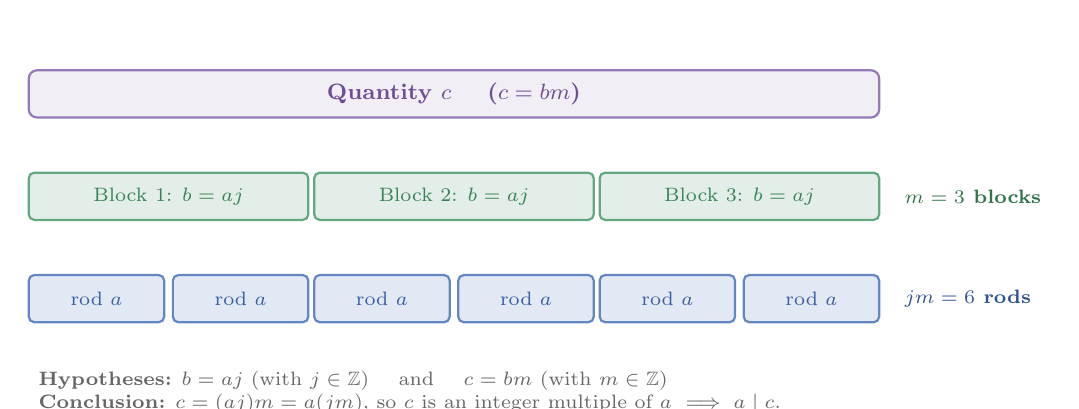
\begin{tikzpicture}[
    font=\small,
    cblock/.style={draw=structurepurple!80, fill=structurepurple!10, rounded corners=3pt, thick},
    bblock/.style={draw=targetgreen!80, fill=targetgreen!15, rounded corners=2pt, thick},
    ablock/.style={draw=sourceblue!80, fill=sourceblue!15, rounded corners=2pt, thick}
]

% Level 1: Entire quantity c
\draw[cblock] (0, 3.2) rectangle (10.8, 3.8);
\node[font=\footnotesize\bfseries, text=structurepurple!90!black] at (5.4, 3.5) {Quantity $c$ \quad ($c = bm$)};

% Level 2: Decomposed into m=3 blocks of size b
\draw[bblock] (0, 1.9) rectangle (3.55, 2.5) node[pos=0.5, font=\scriptsize, text=targetgreen!90!black] {Block 1: $b = aj$};
\draw[bblock] (3.625, 1.9) rectangle (7.175, 2.5) node[pos=0.5, font=\scriptsize, text=targetgreen!90!black] {Block 2: $b = aj$};
\draw[bblock] (7.25, 1.9) rectangle (10.8, 2.5) node[pos=0.5, font=\scriptsize, text=targetgreen!90!black] {Block 3: $b = aj$};
\node[anchor=west, font=\scriptsize\bfseries, text=targetgreen!80!black] at (11.0, 2.2) {$m = 3$ blocks};

% Level 3: Decomposed into j=2 rods of size a per block
\foreach \i in {0, 1, 2} {
    \draw[ablock] (\i*3.625, 0.6) rectangle (\i*3.625 + 1.72, 1.2) node[pos=0.5, font=\scriptsize, text=sourceblue!90!black] {rod $a$};
    \draw[ablock] (\i*3.625 + 1.83, 0.6) rectangle (\i*3.625 + 3.55, 1.2) node[pos=0.5, font=\scriptsize, text=sourceblue!90!black] {rod $a$};
}
\node[anchor=west, font=\scriptsize\bfseries, text=sourceblue!80!black] at (11.0, 0.9) {$jm = 6$ rods};

% Explanatory summary beneath
\node[anchor=north west, font=\scriptsize, text=gray!80!black, align=left] at (0, 0.1) {
    \textbf{Hypotheses:} $b = aj$ (with $j \in \Z$) \quad and \quad $c = bm$ (with $m \in \Z$)\\
    \textbf{Conclusion:} $c = (aj)m = a(jm)$, so $c$ is an integer multiple of $a$ $\implies a \mid c$.
};

\end{tikzpicture}
\caption{Geometric decomposition showing that divisibility is transitive ($a \mid b$ and $b \mid c \implies a \mid c$). The total quantity $c$ is partitioned into $m = 3$ blocks of size $b$. Because $a \mid b$, each individual block of size $b$ is itself partitioned into $j = 2$ rods of size $a$. Nesting these partitions tiles all of $c$ into $jm = 6$ rods of size $a$, certifying that $a \mid c$ with integer witness $k = jm$.}
\label{06:fig-transitivity-tiling}
\end{figure}

\subsection{From single machines to deductive chains}

Up to now, we have tested definitions one at a time. Most theorems, however, connect multiple definitions through conditional claims, such as: ``If an integer $n$ is a multiple of $4$, then $n$ is even.''

In Theorem~\ref{06:thm-divisibility-transitive}, the path from hypothesis to conclusion was direct. But consider the claim: ``If $n^2$ is even, then $n$ is even.'' Unpacking the hypothesis gives $n^2 = 2k$, which yields $n = \sqrt{2k}$---an expression that does not readily reveal the integer factors of $n$.

When a direct algebraic proof is difficult, alternative proof strategies become necessary. In Chapter~7 (\emph{If-Then Statements and Proof Strategy}), we examine the logical structure of conditional statements, exploring contrapositive proof and contradiction.

\subsection{Exercises}

\subsubsection*{Part A: Quick Mental Checks}
\begin{enumerate}
\item For each pair of integers $(a, b)$, decide whether $a \mid b$ is true or false:
\begin{enumerate}[label=(\alph*)]
\item $(7, 42)$
\item $(42, 7)$
\item $(-3, 15)$
\item $(6, 0)$
\item $(0, 6)$
\end{enumerate}

\item Identify the fatal flaw in this student's attempt to prove that the sum of two even integers is even:
\begin{quote}
``Let $x$ and $y$ be even integers. By definition of even, $x = 2k$ and $y = 2k$. Adding them gives $x + y = 2k + 2k = 4k = 2(2k)$. Since $2k$ is an integer, $x + y$ is of the form $2m$, so $x + y$ is even.''
\end{quote}

\item Determine whether each of the following is a \textbf{statement} (an assertion that can be true or false) or a \textbf{term} (an expression denoting a number or object):
\begin{enumerate}[label=(\alph*)]
\item $a \mid b$
\item $a / b$
\item $n = 2k$
\item $2k + 1$
\end{enumerate}
\end{enumerate}

\subsubsection*{Part B: Direct Unpacking and Packaging Practice}
\begin{enumerate}[resume]
\item Prove that the product of two odd integers is odd. Explicitly identify where you unpack the definition of odd and where you package it.
\item Prove that if $a \mid b$ and $a \mid c$, then $a \mid (b + c)$.
\item Prove that if $a \mid b$, then $a \mid (bx)$ for every integer $x$.
\item An integer $n$ is defined to be a \emph{multiple of $4$} if there exists an integer $k$ such that $n = 4k$. Prove that if $n$ is a multiple of $4$, then $n$ is even.
\item A real number $x$ is \emph{rational} ($x \in \Q$) if there exist integers $p, q \in \Z$ with $q \neq 0$ such that $x = p/q$. Prove that if $x, y \in \Q$, then $x + y \in \Q$.
\end{enumerate}

\subsubsection*{Part C: Deeper Exploration}
\begin{enumerate}[resume]
\item Suppose $a, b \in \Z$ are non-zero integers such that $a \mid b$ and $b \mid a$. Prove that $a = b$ or $a = -b$. Where in your argument does the fact that $a$ and $b$ are integers (rather than arbitrary real numbers) play an essential role?
\item An integer $p > 1$ is defined to be \emph{prime} if its only positive divisors are $1$ and $p$. Why do mathematicians deliberately demand $p > 1$, excluding the number $1$ from being prime? (Consider what would happen to the Fundamental Theorem of Arithmetic---which promises that every integer greater than $1$ has a \emph{unique} factorization into primes---if $1$ were included).
\end{enumerate}

\begin{walkbox}
On your next walk, notice how definitions in everyday life (such as ``organic food,'' ``planet,'' or ``full-time employee'') differ from mathematical definitions. When astronomers reclassified Pluto in 2006 by demanding that a planet must ``clear the neighborhood around its orbit,'' they replaced an informal description with explicit classification criteria. What were the specific conditions, and which condition did Pluto fail to satisfy?
\end{walkbox}

\newpage

\section{If-Then Statements and Proof Strategy}
\chapterline

In the previous chapter, we treated definitions as precise classification tools: given an object, they tell us whether it belongs to a class. In mathematics, we connect these conditions into chains of consequence:
\[
P \implies Q.
\]
We call this an \textbf{implication}---a conditional promise that whenever condition $P$ is satisfied, outcome $Q$ is guaranteed to follow. The statement $P$ is called the \textbf{hypothesis} (the starting assumption), and $Q$ is called the \textbf{conclusion} (the promised result).

When you are asked to prove an implication, beginners often make an understandable initial mistake: they look at $P$ and wonder whether it is actually true in the real world. But an implication never asserts that $P$ is true! It makes a conditional promise:
\begin{center}
\itshape ``In any mathematical scenario where $P$ happens to hold, $Q$ is guaranteed to hold as well.''
\end{center}
Think of an airline boarding pass: ``If you hold a ticket for Seat 14B, you may board the plane.'' The airline is not claiming that you hold such a ticket. They are stating a binding rule: hand them a ticket for 14B, and a seat on the plane is guaranteed.

\subsection{Implication as geometric containment}

The cleanest way to visualize an implication is through the geometry of sets. Let $U$ be the universe of all possible scenarios, let $P$ be the set of scenarios where the hypothesis holds, and let $Q$ be the set of scenarios where the conclusion holds.

The assertion $P \implies Q$ means precisely that \textbf{$P$ is a subset of $Q$} ($P \subseteq Q$).

\begin{center}
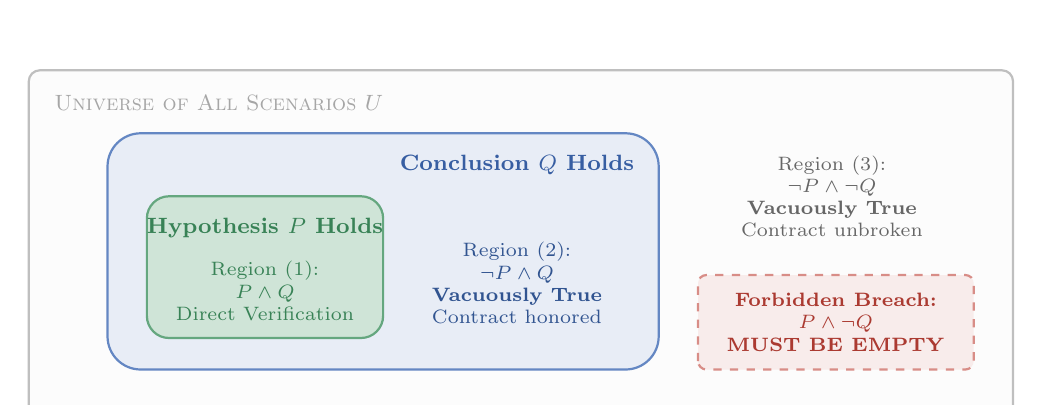
\begin{tikzpicture}[
    font=\small,
    universe/.style={draw=gray!50, fill=gray!2, rounded corners=4pt, thick},
    concl/.style={draw=sourceblue!80, fill=sourceblue!12, rounded corners=12pt, thick},
    hypo/.style={draw=targetgreen!80, fill=targetgreen!25, rounded corners=8pt, thick}
]

% Universe Box
\draw[universe] (0, 0) rectangle (12.5, 4.4);
\node[anchor=north west, font=\footnotesize\scshape, text=gray!70] at (0.2, 4.2) {Universe of All Scenarios $U$};

% Conclusion Region Q
\draw[concl] (1.0, 0.6) rectangle (8.0, 3.6);
\node[font=\footnotesize\bfseries, text=sourceblue!90!black] at (6.2, 3.2) {Conclusion $Q$ Holds};

% Hypothesis Region P (nested entirely inside Q)
\draw[hypo] (1.5, 1.0) rectangle (4.5, 2.8);
\node[font=\footnotesize\bfseries, text=targetgreen!90!black] at (3.0, 2.4) {Hypothesis $P$ Holds};
\node[font=\scriptsize, text=targetgreen!90!black, align=center] at (3.0, 1.6) {Region (1):\\$P \land Q$\\Direct Verification};

% Vacuous region inside Q but outside P
\node[font=\scriptsize, text=sourceblue!80!black, align=center] at (6.2, 1.7) {Region (2):\\$\neg P \land Q$\\\textbf{Vacuously True}\\Contract honored};

% Vacuous region outside both P and Q
\node[font=\scriptsize, text=gray!80!black, align=center] at (10.2, 2.8) {Region (3):\\$\neg P \land \neg Q$\\\textbf{Vacuously True}\\Contract unbroken};

% Forbidden breach region (highlighted outside)
\draw[draw=trapred!60, fill=trapred!10, rounded corners=3pt, thick, dashed] (8.5, 0.6) rectangle (12.0, 1.8);
\node[font=\scriptsize\bfseries, text=trapred!90!black, align=center] at (10.25, 1.2) {Forbidden Breach:\\$P \land \neg Q$\\\textbf{MUST BE EMPTY}};

\end{tikzpicture}
\end{center}

This geometry reveals how truth behaves:
\begin{itemize}
\item \textbf{Region 1 ($P$ is true, $Q$ is true)}: You stand inside $P$. Because the boundary of $P$ is nested entirely inside $Q$, you are automatically inside $Q$. For example, if $n$ is a multiple of $4$, then $n$ is automatically even. Both hypothesis and conclusion hold; the promise is fulfilled.
\item \textbf{Region 2 ($\neg P$ holds, $Q$ is true)}: You stand inside $Q$, but outside $P$. For example, the number $6$ is even, but it is not a multiple of $4$. Has the promise ``if a multiple of $4$, then even'' been broken? Not at all. The promise said nothing about what happens to numbers that are not multiples of $4$.
\item \textbf{Region 3 ($\neg P$ holds, $\neg Q$ holds)}: You stand outside both $P$ and $Q$. For example, $7$ is neither a multiple of $4$ nor even. Again, no promise was broken.
\item \textbf{The Forbidden Region ($P$ is true, $\neg Q$ holds)}: This would be a point inside $P$ but outside $Q$---for example, an integer that is a multiple of $4$ yet odd. If even a single such point existed, the implication $P \implies Q$ would be false. Saying that $P \implies Q$ is true means this region contains no points.
\end{itemize}

\subsection{Vacuous truth: promises about empty conditions}

The fact that $P \implies Q$ is considered true whenever $P$ is false is known as \textbf{vacuous truth}---a conditional promise that is declared true simply because its starting condition is impossible or never satisfied. Beginners often find this unsettling at first encounter. Consider the statement:
\begin{quote}
``If an integer is both a multiple of $4$ and an odd number, then that integer is purple.''
\end{quote}
Is this statement true? In mathematical logic, the answer is an unqualified \textbf{yes}. 

Why? Because an integer that is simultaneously a multiple of $4$ and odd does not exist. The hypothesis describes the empty set $\emptyset$---the unique set containing zero elements. To catch someone breaking an if-then promise, you must bring forward a real counterexample that fulfills premise $P$ while violating conclusion $Q$. Because no one can ever produce an odd multiple of $4$, no one can ever catch the promise in a breach.

\begin{recoverybox}
\textbf{Pause and think:} Suppose an instructor announces: ``If you score $105\%$ on the final exam, you will receive an A+.'' You take the exam, earn $88\%$, and receive a B. Did the instructor break their promise or lie to you?

\emph{Answer:} No. The promise was conditioned on scoring $105\%$. Because you never fulfilled that condition, the instructor had no obligation to award the A+, and no breach of contract occurred. In mathematics, unbroken promises are classified as true.
\end{recoverybox}

\begin{historybox}
Around 300 BCE, two Greek philosophers of the Megarian school---an ancient philosophical circle centered in Megara devoted to logic puzzles and paradoxes---sparked a debate over conditionals that lasted for more than two millennia. Philo of Megara and his teacher Diodorus Cronus asked a direct question: what does it mean for a promise of the form ``If $P$, then $Q$'' to be true when the condition $P$ does not happen?

Philo proposed an answer that startled the ancient world: an implication is true in every single case except when the premise $P$ is true and the outcome $Q$ is false. Under Philo's rule, whenever $P$ is false, the implication is automatically true---what modern logicians call \emph{material implication}, the rule that evaluates a conditional purely by the truth or falsehood of its parts, without requiring any real-world cause connecting them. Diodorus Cronus and the Stoic philosopher Chrysippus vehemently objected, arguing that an authentic conditional requires an intrinsic causal or logical bond. To their ears, calling ``If $2 + 2 = 5$, then the Moon is made of green cheese'' true seemed to mock human intuition. Bertrand Russell later dramatized the Megarian logic when challenged to prove that a false premise implies anything: if $1 = 0$, adding $1$ yields $2 = 1$; the collection containing Bertrand Russell and the Pope has two members, but $2 = 1$, so the collection has one member, proving that Russell and the Pope are one and the same person!

In 1879, Gottlob Frege and later Bertrand Russell and Alfred North Whitehead in \emph{Principia Mathematica} (1910) recognized that Philo's material implication was indispensable for formalizing mathematics. By decoupling mathematical proofs from subjective human feelings of ``relevance,'' mathematical logic could be executed as a rigorous, symbolic calculus. Without vacuous truth, modern set theory would instantly stall: we could not prove that the empty set is a subset of every set ($\emptyset \subseteq A$), nor could computer programs execute conditional branching instructions reliably.
\end{historybox}

In set theory, vacuous truth is the exact reason why the empty set $\emptyset$ is a subset of every set:
\[
\emptyset \subseteq A \quad \text{for every set } A.
\]
Recall the definition of subset: $S \subseteq A$ means that for every object $x$, if $x \in S$, then $x \in A$. When $S = \emptyset$, the hypothesis ``$x \in \emptyset$'' is false for every object in the mathematical universe. The condition is vacuously satisfied for every element, and the containment holds without exception.

\subsection{The trap of the converse and inverse}

Once you have an implication $P \implies Q$, there are three other conditional statements that can be formed by rearranging and negating its pieces:

\begin{enumerate}
\item \textbf{The Converse ($Q \implies P$)}: Swap the hypothesis and conclusion.
\item \textbf{The Inverse ($\neg P \implies \neg Q$)}: Negate both sides without swapping.
\item \textbf{The Contrapositive ($\neg Q \implies \neg P$)}: Swap both sides \emph{and} negate both sides.
\end{enumerate}

To see how these differ, let us test them on a simple arithmetic statement where $P$ is ``$x = 3$'' and $Q$ is ``$x^2 = 9$'', working with real numbers:
\begin{itemize}
\item \textbf{Original ($P \implies Q$)}: ``If $x = 3$, then $x^2 = 9$.'' \\
\emph{Status:} \textbf{True.} $3^2 = 9$.
\item \textbf{Converse ($Q \implies P$)}: ``If $x^2 = 9$, then $x = 3$.'' \\
\emph{Status:} \textbf{False!} If $x^2 = 9$, $x$ could equal $-3$.
\item \textbf{Inverse ($\neg P \implies \neg Q$)}: ``If $x \neq 3$, then $x^2 \neq 9$.'' \\
\emph{Status:} \textbf{False!} Setting $x = -3$ satisfies $x \neq 3$, yet $x^2 = 9$.
\item \textbf{Contrapositive ($\neg Q \implies \neg P$)}: ``If $x^2 \neq 9$, then $x \neq 3$.'' \\
\emph{Status:} \textbf{True.} If the square is not $9$, the number could not possibly have been $3$.
\end{itemize}

\begin{center}
\small
\begin{tabular}{lll}
\toprule
\textbf{Statement Form} & \textbf{Symbolic Logic} & \textbf{Truth Relation to $P \implies Q$} \\
\midrule
Original Implication & $P \implies Q$ & The baseline claim \\
Contrapositive & $\neg Q \implies \neg P$ & \textbf{Logically equivalent} (identical truth value) \\
Converse & $Q \implies P$ & \textbf{Independent statement} (may be true or false) \\
Inverse & $\neg P \implies \neg Q$ & \textbf{Equivalent to converse} (independent of original) \\
\bottomrule
\end{tabular}
\end{center}

Notice that the inverse ($\neg P \implies \neg Q$) is the contrapositive of the converse ($Q \implies P$). That is why the inverse and converse always share the exact same truth value. But neither of them has any logical obligation to agree with the original statement!

The square of conditionals in the diagram below summarizes these relationships: diagonal pairs share identical truth values, while horizontal and vertical moves lead to independent claims.

\begin{center}
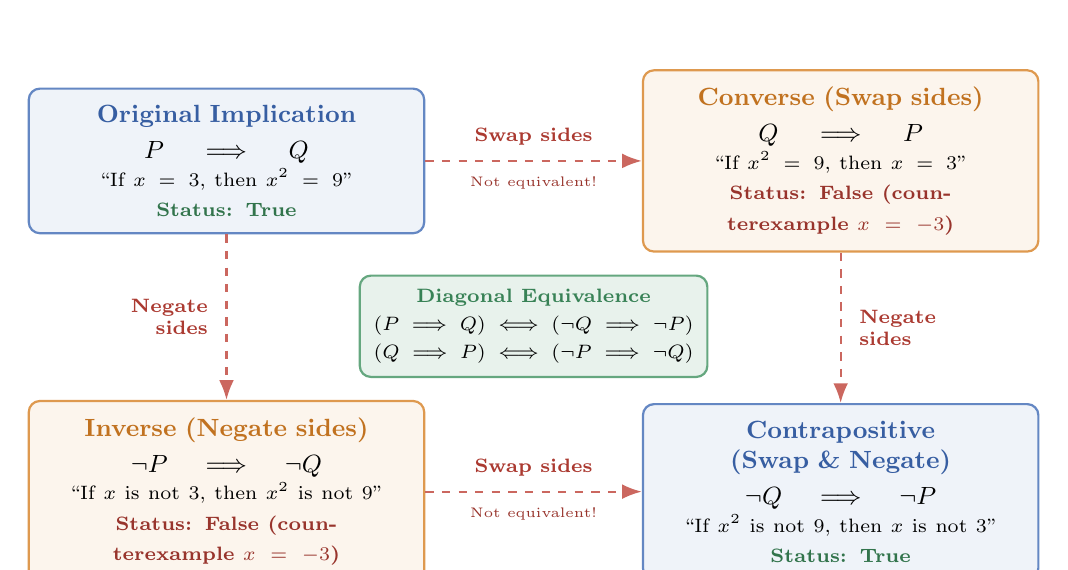
\begin{tikzpicture}[
    font=\small,
    boxorig/.style={draw=sourceblue!80, fill=sourceblue!8, rounded corners=4pt, thick, text width=4.6cm, inner sep=6pt, align=center},
    boxconv/.style={draw=quotientorange!80, fill=quotientorange!8, rounded corners=4pt, thick, text width=4.6cm, inner sep=6pt, align=center},
    linkdash/.style={-{Latex[length=2.5mm]}, thick, trapred!80, dashed}
]

% Top-Left: Original
\node[boxorig] (orig) at (0, 3.4) {
    \textbf{\color{sourceblue!90!black}Original Implication}\\[2pt]
    $P \implies Q$\\[2pt]
    \scriptsize ``If $x = 3$, then $x^2 = 9$''\\\textbf{\color{targetgreen!80!black}Status: True}
};

% Top-Right: Converse
\node[boxconv] (conv) at (7.8, 3.4) {
    \textbf{\color{quotientorange!90!black}Converse (Swap sides)}\\[2pt]
    $Q \implies P$\\[2pt]
    \scriptsize ``If $x^2 = 9$, then $x = 3$''\\\textbf{\color{trapred!80!black}Status: False (counterexample $x=-3$)}
};

% Bottom-Left: Inverse
\node[boxconv] (inv) at (0, -0.8) {
    \textbf{\color{quotientorange!90!black}Inverse (Negate sides)}\\[2pt]
    $\neg P \implies \neg Q$\\[2pt]
    \scriptsize ``If $x$ is not $3$, then $x^2$ is not $9$''\\\textbf{\color{trapred!80!black}Status: False (counterexample $x=-3$)}
};

% Bottom-Right: Contrapositive
\node[boxorig] (contra) at (7.8, -0.8) {
    \textbf{\color{sourceblue!90!black}Contrapositive (Swap \& Negate)}\\[2pt]
    $\neg Q \implies \neg P$\\[2pt]
    \scriptsize ``If $x^2$ is not $9$, then $x$ is not $3$''\\\textbf{\color{targetgreen!80!black}Status: True}
};

% Horizontal dashed arrows (non-equivalence)
\draw[linkdash] (orig.east) -- node[above=2pt, font=\scriptsize\bfseries, text=trapred!90!black]{Swap sides} node[below=2pt, font=\tiny, text=trapred!80!black]{Not equivalent!} (conv.west);
\draw[linkdash] (inv.east) -- node[above=2pt, font=\scriptsize\bfseries, text=trapred!90!black]{Swap sides} node[below=2pt, font=\tiny, text=trapred!80!black]{Not equivalent!} (contra.west);

% Vertical dashed arrows (non-equivalence)
\draw[linkdash] (orig.south) -- node[left=3pt, font=\scriptsize\bfseries, text=trapred!90!black, align=right]{Negate\\sides} (inv.north);
\draw[linkdash] (conv.south) -- node[right=3pt, font=\scriptsize\bfseries, text=trapred!90!black, align=left]{Negate\\sides} (contra.north);

% Central equivalence banner
\node[draw=targetgreen!80, fill=targetgreen!12, rounded corners=4pt, thick, inner sep=5pt, align=center, font=\scriptsize] (center) at (3.9, 1.3) {
    \textbf{\color{targetgreen!90!black}Diagonal Equivalence}\\[2pt]
    $(P \implies Q) \iff (\neg Q \implies \neg P)$\\[2pt]
    $(Q \implies P) \iff (\neg P \implies \neg Q)$
};

\end{tikzpicture}
\end{center}

\begin{trapbox}
\textbf{The Converse Fallacy}: One of the most common errors in all of mathematics is confusing an implication with its converse. In casual conversation, people say ``If it is raining, the sidewalk is wet'' and loosely assume that a wet sidewalk implies rain. But a sprinkler could have caused it! Never assume that proving $P \implies Q$ gives you any license to use $Q \implies P$.
\end{trapbox}

What happens when an implication and its converse are \emph{both} true? In that case, the two statements are logically equivalent, and we write:
\[
P \iff Q \quad (\text{``}P \text{ if and only if } Q\text{''}, \text{ often abbreviated } P \text{ iff } Q).
\]
A statement of the form $P \iff Q$ is called a \textbf{biconditional}---a two-way promise. Whenever you see a theorem framed as ``$P$ if and only if $Q$,'' you are being given two separate mathematical tasks:
\begin{enumerate}
\item \textbf{Forward direction ($\implies$)}: Assume $P$, deduce $Q$.
\item \textbf{Backward direction ($\impliedby$)}: Assume $Q$, deduce $P$ (or prove its contrapositive: assume $\neg P$, deduce $\neg Q$).
\end{enumerate}

\begin{recoverybox}
\textbf{Pause and think:} State the converse of: ``If a number is divisible by $10$, then it is divisible by $5$.'' Is the converse true?

\emph{Answer:} The converse is: ``If a number is divisible by $5$, then it is divisible by $10$.'' This converse is false: for instance, $15$ is divisible by $5$, but not by $10$. The original implication holds, but the converse fails.
\end{recoverybox}

\subsection{Three standard proof strategies}

When proving an implication $P \implies Q$, there are three standard approaches:

\begin{center}
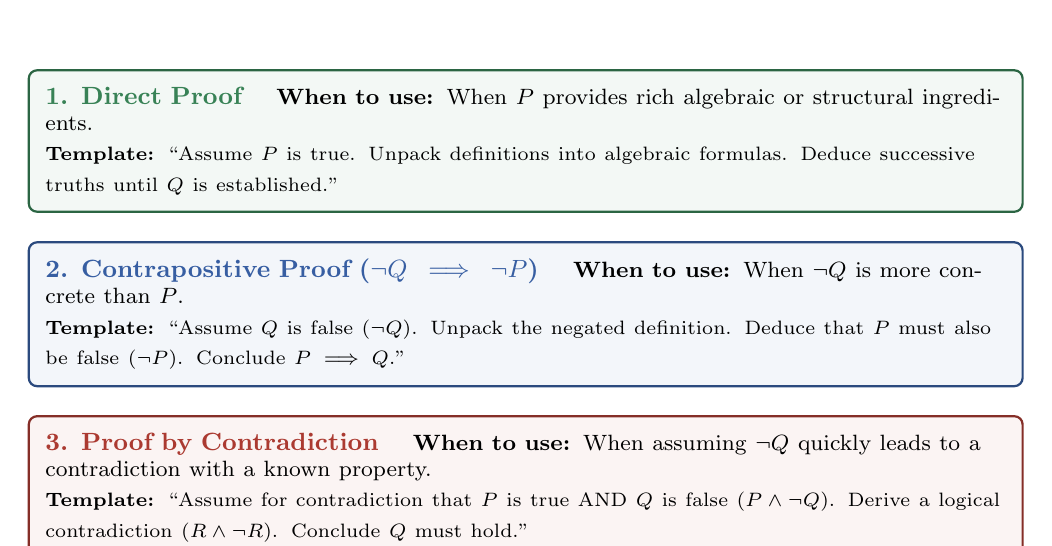
\begin{tikzpicture}[
    font=\small,
    plan/.style={draw=#1!70!black, fill=#1!6, rounded corners=3pt, thick, text width=12.2cm, inner sep=6pt}
]

% Plan 1: Direct Proof
\node[plan=targetgreen] (p1) at (0, 3.2) {
    \textbf{\color{targetgreen!90!black}1. Direct Proof} \quad \footnotesize\textbf{When to use:} When $P$ provides rich algebraic or structural ingredients.\\
    \scriptsize
    \textbf{Template:} ``Assume $P$ is true. Unpack definitions into algebraic formulas. Deduce successive truths until $Q$ is established.''
};

% Plan 2: Contrapositive
\node[plan=sourceblue] (p2) at (0, 1.0) {
    \textbf{\color{sourceblue!90!black}2. Contrapositive Proof ($\neg Q \implies \neg P$)} \quad \footnotesize\textbf{When to use:} When $\neg Q$ is more concrete than $P$.\\
    \scriptsize
    \textbf{Template:} ``Assume $Q$ is false ($\neg Q$). Unpack the negated definition. Deduce that $P$ must also be false ($\neg P$). Conclude $P \implies Q$.''
};

% Plan 3: Contradiction
\node[plan=trapred] (p3) at (0, -1.2) {
    \textbf{\color{trapred!90!black}3. Proof by Contradiction} \quad \footnotesize\textbf{When to use:} When assuming $\neg Q$ quickly leads to a contradiction with a known property.\\
    \scriptsize
    \textbf{Template:} ``Assume for contradiction that $P$ is true AND $Q$ is false ($P \land \neg Q$). Derive a logical contradiction ($R \land \neg R$). Conclude $Q$ must hold.''
};

\end{tikzpicture}
\end{center}

\subsection{Strategy 1: The direct route and the forward-backward method}

In a direct proof, you take premise $P$ as given and deduce conclusion $Q$ through a chain of lawful steps. But how do you find those steps when staring at a blank page?

Beginners often imagine that mathematicians discover proofs in a single forward pass, writing down line 1, then line 2, all the way to the end. In reality, finding a proof is often a two-directional process: the \textbf{forward-backward method}.

Before writing the final proof, split your scratchpad into two columns:
\begin{enumerate}
\item \textbf{The Forward Column (What do I know?)}: Start with hypothesis $P$. Unpack its definitions into concrete algebraic tools. Ask: \emph{``What facts can I extract immediately from this starting point?''}
\item \textbf{The Backward Column (What do I need?)}: Look at conclusion $Q$. Unpack what it would take to justify $Q$. Ask: \emph{``What statement, if I could prove it, would be sufficient to declare $Q$ true?''}
\item \textbf{Connecting the Two Sides}: Manipulate the forward equations until they match the form required by the backward target. Once the two ends connect, write down the final proof from start to finish, presenting a clean deductive argument.
\end{enumerate}

Let us see how this method works on a concrete example.

\begin{theorem}
Let $n \in \Z$. If $n$ is odd, then $5n + 3$ is even.
\end{theorem}

\begin{proof}[Scratchwork and Discovery]
\textbf{Forward:} The hypothesis is that $n$ is odd. Unpacking the definition of odd from Chapter~6 gives:
\[
n = 2k + 1 \quad \text{for some integer } k.
\]
\textbf{Backward:} The target conclusion is that $5n + 3$ is even. Unpacking the definition of even tells us our destination: we must show that
\[
5n + 3 = 2m \quad \text{for some integer } m.
\]
\textbf{Connecting the bridge:} We substitute the forward expression $n = 2k + 1$ into $5n + 3$:
\[
5n + 3 = 5(2k + 1) + 3 = 10k + 5 + 3 = 10k + 8 = 2(5k + 4).
\]
Because $k$ is an integer, $5k + 4$ is an integer. Setting $m = 5k + 4$ delivers the exact form $2m$ demanded by the definition of an even integer.
\end{proof}

The diagram below visualizes this strategy: forward unpacking and backward target-setting meet once the expression is factored into the required form.

\begin{center}
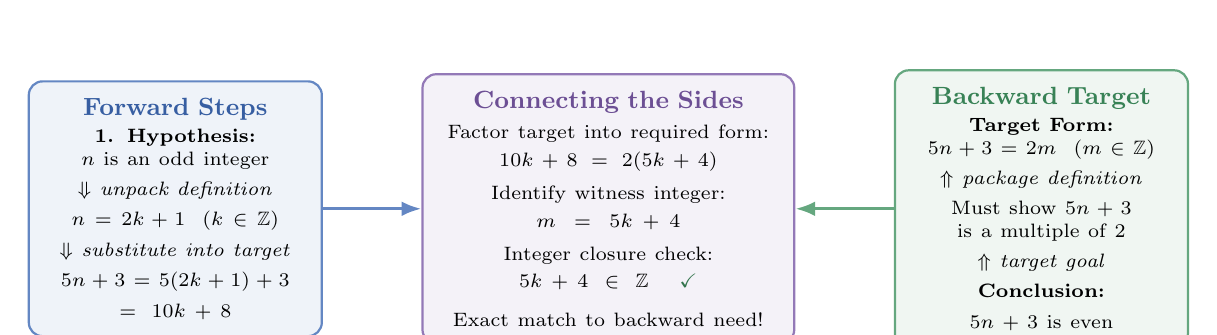
\begin{tikzpicture}[
    font=\small,
    front/.style={draw=#1!80, fill=#1!8, rounded corners=5pt, thick, text width=3.3cm, inner sep=6pt, align=center},
    steparrow/.style={-{Latex[length=2.5mm]}, very thick}
]

% Left: Forward Column
\node[front=sourceblue] (fwd) at (1.1, 0) {
    \textbf{\color{sourceblue!90!black}Forward Steps}\\[2pt]
    \scriptsize
    \textbf{1. Hypothesis:}\\
    $n$ is an odd integer\\[3pt]
    $\Downarrow$ \emph{unpack definition}\\[3pt]
    $n = 2k + 1$ \ ($k \in \Z$)\\[3pt]
    $\Downarrow$ \emph{substitute into target}\\[3pt]
    $5n + 3 = 5(2k + 1) + 3$\\
    $= 10k + 8$
};

% Center: The Bridge
\node[front=structurepurple, text width=4.3cm] (br) at (6.6, 0) {
    \textbf{\color{structurepurple!90!black}Connecting the Sides}\\[3pt]
    \scriptsize
    Factor target into required form:\\[2pt]
    $10k + 8 = 2(5k + 4)$\\[4pt]
    Identify witness integer:\\[2pt]
    $m = 5k + 4$\\[4pt]
    Integer closure check:\\[2pt]
    $5k + 4 \in \Z$ \quad \textbf{\color{targetgreen!80!black}\checkmark}\\[3pt]
    Exact match to backward need!
};

% Right: Backward Column
\node[front=targetgreen] (bwd) at (12.1, 0) {
    \textbf{\color{targetgreen!90!black}Backward Target}\\[2pt]
    \scriptsize
    \textbf{Target Form:}\\
    $5n + 3 = 2m$ \ ($m \in \Z$)\\[3pt]
    $\Uparrow$ \emph{package definition}\\[3pt]
    Must show $5n + 3$ is a multiple of $2$\\[3pt]
    $\Uparrow$ \emph{target goal}\\[3pt]
    \textbf{Conclusion:}\\
    $5n + 3$ is even
};

% Connecting Horizontal Arrows
\draw[steparrow, sourceblue!80] (fwd.east) -- (br.west);
\draw[steparrow, targetgreen!80] (bwd.west) -- (br.east);

\end{tikzpicture}
\end{center}

Now we write the polished formal proof:

\begin{proof}
Assume $n$ is an odd integer.

By definition of an odd integer, there exists an integer $k$ such that $n = 2k + 1$. Substituting this expression into $5n + 3$, we have:
\[
5n + 3 = 5(2k + 1) + 3 = 10k + 5 + 3 = 10k + 8 = 2(5k + 4).
\]
Let $m = 5k + 4$. Since $k \in \Z$, the quantity $m$ is an integer by closure of the integers under addition and multiplication. 

Thus, $5n + 3 = 2m$ for an integer $m$. By definition, $5n + 3$ is even.
\end{proof}

Every step is accounted for: we unpacked the definition of odd, carried out the algebra, checked integer closure, and verified the definition of an even integer.

\subsection{Strategy 2: Contrapositive proof}

Direct proof works well when the hypothesis $P$ gives concrete algebraic formulas to manipulate. But what happens when the hypothesis is awkward to unpack?

Consider the following innocent-looking theorem:
\begin{theorem}
Let $n \in \Z$. If $n^2$ is even, then $n$ is even.
\end{theorem}

Let us attempt a direct proof. We assume $n^2$ is even. Unpacking the definition gives:
\[
n^2 = 2k \quad \text{for some integer } k.
\]
Now we want to deduce that $n$ is even. To isolate $n$, we take square roots:
\[
n = \sqrt{2k}.
\]
Here the direct approach stalls. Is $\sqrt{2k}$ an integer? Squaring an integer is straightforward, but taking square roots leaves divisibility unclear.

This is the exact moment to pivot to the \textbf{contrapositive}:
\[
\neg Q \implies \neg P.
\]
Recall that for any statements $P$ and $Q$, the implication $P \implies Q$ is logically equivalent to its contrapositive:
\[
(P \implies Q) \iff (\neg Q \implies \neg P).
\]
Look back at the Euler diagram. To say that $P$ is inside $Q$ ($P \subseteq Q$) is geometrically identical to saying that if you stand outside $Q$, you are guaranteed to be standing outside $P$ ($Q^c \subseteq P^c$). If you are outside the big circle, you cannot possibly be inside the small circle! If a bedroom is inside an apartment, someone standing outside the apartment is guaranteed not to be in the bedroom.

Now let us apply the contrapositive to our theorem. The conclusion is ``$n$ is even,'' so its negation $\neg Q$ is ``$n$ is not even'' (meaning $n$ is odd). The hypothesis is ``$n^2$ is even,'' so its negation $\neg P$ is ``$n^2$ is odd.'' The contrapositive claim is:
\begin{center}
\itshape ``If $n$ is odd, then $n^2$ is odd.''
\end{center}
Instead of starting with $n^2$ and taking square roots, we start with $n$ and square it. The algebraic direction is straightforward.

\begin{proof}
We prove the theorem by contrapositive: if $n$ is not even, then $n^2$ is not even.

For integers, an integer that is not even is odd. Assume $n$ is odd. By definition, there exists an integer $k$ such that $n = 2k + 1$. Squaring both sides:
\[
n^2 = (2k + 1)^2 = 4k^2 + 4k + 1 = 2(2k^2 + 2k) + 1.
\]
Because $k$ is an integer, $m = 2k^2 + 2k$ is an integer by closure under addition and multiplication. Thus $n^2 = 2m + 1$, which means $n^2$ is odd.

We have established that if $n$ is odd, then $n^2$ is odd. Because an implication is logically equivalent to its contrapositive, it follows that if $n^2$ is even, then $n$ must be even.
\end{proof}

\subsection{Choosing a proof strategy: direct, contrapositive, or contradiction}

When proving an implication, which strategy should you choose? Here are standard guidelines:

\begin{itemize}
\item \textbf{Use Direct Proof} when hypothesis $P$ provides clear algebraic formulas (such as $n$ is odd, $a \mid b$, or $x, y \in \Q$) that you can unpack and substitute directly into the conclusion. If the forward path moves naturally toward $Q$, direct proof is the cleanest and most transparent route.
\item \textbf{Use Contrapositive} when:
\begin{itemize}
\item The conclusion $Q$ is simpler to unpack than hypothesis $P$ (for example, starting from $n$ is far easier than starting from $n^2$).
\item The conclusion contains a negative assertion, such as ``$x$ is irrational'' or ``$x \neq 0$.'' Negating $\neg Q$ transforms a negative condition into a positive algebraic equation ($x \in \Q$ or $x = 0$) that gives you immediate formulas to manipulate.
\end{itemize}
\item \textbf{Use Proof by Contradiction} when neither direct nor contrapositive paths offer a foothold. Direct and contrapositive proofs start from what is given and deduce consequences forward. Proof by contradiction assumes both the hypothesis and the negation of the conclusion ($P \land \neg Q$), reasoning from there until reaching a contradiction ($R \land \neg R$).
\end{itemize}

Contradiction is especially useful when a theorem makes a negative claim with no algebraic hypothesis to unpack---such as proving that $\sqrt{2}$ is irrational, or that the primes never end.

In Chapter~8 (\emph{Proof by Contradiction: Power and Danger}), we examine this method in detail: how assuming the opposite uncovers contradictions, classic examples from ancient Greece to modern analysis, and how to avoid common pitfalls.

\subsection{Exercises}

\subsubsection*{Part A: Warm-Up Mental Checks}
\begin{enumerate}
\item Evaluate the truth value of each implication:
\begin{enumerate}
\item If $2 + 2 = 5$, then $3 \times 3 = 9$.
\item If $2 + 2 = 4$, then $3 \times 3 = 10$.
\item If $2 + 2 = 5$, then $3 \times 3 = 10$.
\end{enumerate}
\item For each statement, write down its converse, inverse, and contrapositive:
\begin{enumerate}
\item If an integer $n$ is a multiple of $8$, then $n$ is a multiple of $4$.
\item If a real number $x$ satisfies $x > 3$, then $x^2 > 9$.
\end{enumerate}
\item Identify the logical error in the following argument: ``Every differentiable function is continuous. Since $f(x) = |x|$ is continuous at $x = 0$, it must be differentiable at $x = 0$.''
\end{enumerate}

\subsubsection*{Part B: Routine Practice}
\begin{enumerate}[resume]
\item State the contrapositive and the negation of each implication:
\begin{enumerate}
\item If $x > 2$, then $x^2 > 4$.
\item If a triangle is equilateral, then it is equiangular.
\item If an integer $n$ is divisible by $6$, then $n$ is divisible by $2$ and by $3$.
\end{enumerate}
\item Prove each statement using a direct proof. Explicitly label where you unpack definitions and where you package your conclusion:
\begin{enumerate}
\item For $n \in \Z$, if $n$ is even, then $3n^2 - 5n + 6$ is even.
\item For $a, b, c \in \Z$, if $a \mid b$ and $a \mid c$, then $a \mid (2b + 3c)$.
\end{enumerate}
\end{enumerate}

\subsubsection*{Part C: Contrapositive Proofs}
\begin{enumerate}[resume]
\item Prove each statement by contrapositive:
\begin{enumerate}
\item For $n \in \Z$, if $3n + 2$ is odd, then $n$ is odd.
\item For real numbers $x, y$, if $x + y > 10$, then $x > 5$ or $y > 5$.
\item For an integer $n$, if $n^2 - 1$ is not divisible by $4$, then $n$ is even.
\end{enumerate}
\end{enumerate}

\subsubsection*{Part D: Deeper Challenges}
\begin{enumerate}[resume]
\item \textbf{A Biconditional Theorem:} Let $n \in \Z$. Prove that $n$ is even if and only if $n^2$ is even. (Explicitly present both the forward direction $\implies$ and the backward direction $\impliedby$, noting where the direct route and the contrapositive route each apply.)
\item \textbf{Rational and Irrational Numbers:} Recall that a real number $r$ is rational ($r \in \Q$) if $r = a/b$ for integers $a, b$ with $b \neq 0$, and irrational otherwise. Prove that if $x$ is irrational and $r$ is a non-zero rational number, then $r \cdot x$ is irrational. (Why does the contrapositive make working with irrational numbers more direct?)
\item If $x$ is irrational, prove that $-x$ is irrational.
\end{enumerate}

\newpage

\section{Proof by Contradiction: Power and Danger}
\chapterline

Proof by contradiction is one of the most powerful and psychologically dramatic tools in mathematics. When direct attacks stall and contrapositive restructuring offers no purchase, contradiction allows you to assume the exact opposite of what you hope to prove, step inside that hypothetical counter-world, and walk forward until logical reality shatters.

The English mathematician G.~H.~Hardy famously described it in \emph{A Mathematician's Apology}:
\begin{quote}
``Reductio ad absurdum, which Euclid loved so much, is one of a mathematician's finest weapons. It is a far finer gambit than any chess gambit: a chess player may offer the sacrifice of a pawn or even a piece, but a mathematician offers the game.''
\end{quote}

Yet because of its dramatic power, beginners frequently misuse it. Contradiction is not an excuse to generate vague fog until something ``feels wrong.'' A contradiction proof succeeds only when two crystal-clear, mutually exclusive mathematical facts collide head-on: $A \land \neg A$.

\begin{historybox}
Around 500 BCE, the followers of Pythagoras lived by a mystical doctrine: ``All is Number.'' To the Pythagoreans, every relationship in nature, music, and geometry could be expressed as a ratio of whole numbers. When studying a right triangle with legs of length $1$, they sought two whole numbers $a$ and $b$ whose ratio $a/b$ measured the hypotenuse.

According to ancient legend, a member named Hippasus of Metapontum realized that assuming such a fraction exists leads to an inescapable trap: the numerator $a$ must be even, which forces the denominator $b$ to be even, destroying the assumption that the fraction was reduced to lowest terms. The diagonal was incommensurable with the side. Legend has it that the brotherhood was so unsettled by this scandal that they drowned Hippasus at sea to bury the secret. Yet two centuries later, Euclid recorded this exact parity contradiction in Book X of the \emph{Elements}, alongside his legendary proof that prime numbers never run out.

In the early twentieth century, the Dutch mathematician L.E.J. Brouwer criticized proof by contradiction for being non-constructive. Brouwer argued that proving an object exists by showing that its absence causes a contradiction leaves you empty-handed: it proves non-existence is impossible, but offers no recipe or algorithm to construct the object. In modern computer science, constructive proofs are prized because algorithms require tangible witnesses. Yet proof by contradiction remains our premier weapon for establishing impossibility results: proving that no fraction can equal $\sqrt{2}$, and no finite list contains all primes.
\end{historybox}

\subsection{Visualizing the split reality}

\begin{center}
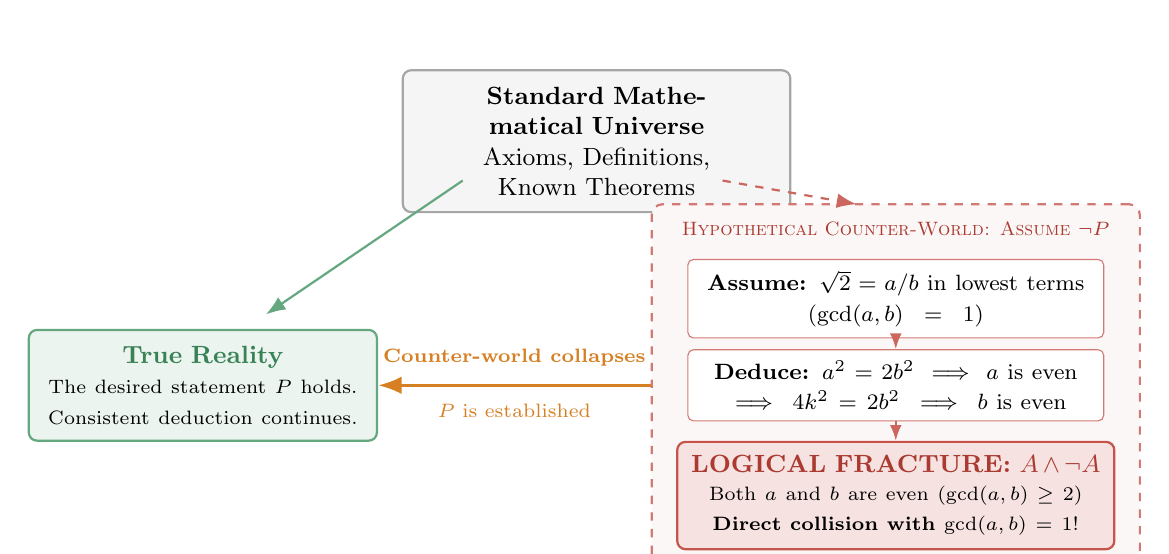
\begin{tikzpicture}[
    font=\small,
    rootnode/.style={draw=gray!70, fill=gray!8, rounded corners=3pt, thick, text width=4.5cm, align=center, inner sep=6pt},
    realnode/.style={draw=targetgreen!80, fill=targetgreen!10, rounded corners=3pt, thick, text width=4.0cm, align=center, inner sep=6pt},
    counterbox/.style={draw=trapred!70, fill=trapred!4, rounded corners=4pt, dashed, thick, inner sep=8pt},
    cnode/.style={draw=trapred!70, fill=white, rounded corners=2pt, text width=5.0cm, align=center, inner sep=4pt}
]

% Root Node
\node[rootnode] (root) at (2.2, 4.4) {\textbf{Standard Mathematical Universe}\\Axioms, Definitions, Known Theorems};

% Real Branch (Left)
\node[realnode] (real) at (-2.8, 1.3) {
    \textbf{\color{targetgreen!90!black}True Reality}\\[0.3em]
    \scriptsize The desired statement $P$ holds.\\Consistent deduction continues.
};
\draw[-{Latex[length=2.5mm]}, thick, targetgreen!80] (0.5, 3.9) -- (-2.0, 2.2);

% Counter-World Box (Right)
\node[counterbox, minimum width=6.2cm, minimum height=4.6cm] (cbox) at (6.0, 1.3) {};
\node[anchor=north, font=\scriptsize\scshape, text=trapred!90!black] at (6.0, 3.5) {Hypothetical Counter-World: Assume $\neg P$};

\draw[-{Latex[length=2.5mm]}, thick, trapred!80, dashed] (3.8, 3.9) -- (5.5, 3.6);

% Nodes inside Counter-World
\node[cnode] (step1) at (6.0, 2.4) {\footnotesize \textbf{Assume:} $\sqrt{2} = a/b$ in lowest terms\\($\gcd(a, b) = 1$)};
\node[cnode] (step2) at (6.0, 1.3) {\footnotesize \textbf{Deduce:} $a^2 = 2b^2 \implies a$ is even\\$\implies 4k^2 = 2b^2 \implies b$ is even};

% Collision Node
\node[draw=trapred!90, fill=trapred!15, rounded corners=3pt, thick, text width=5.2cm, align=center, inner sep=5pt] (rupture) at (6.0, -0.1) {
    \textbf{\color{trapred!90!black}LOGICAL FRACTURE: $A \land \neg A$}\\[0.2em]
    \scriptsize Both $a$ and $b$ are even ($\gcd(a, b) \ge 2$)\\
    \textbf{Direct collision with} $\gcd(a, b) = 1$!
};

\draw[-{Latex[length=2mm]}, thick, trapred!80] (step1) -- (step2);
\draw[-{Latex[length=2mm]}, thick, trapred!80] (step2) -- (rupture);

% Elimination arrow pointing back to Real
\draw[-{Latex[length=3mm]}, very thick, quotientorange] (cbox.west) -- node[above=3pt, font=\scriptsize\bfseries, text=quotientorange]{Counter-world collapses} node[below=3pt, font=\scriptsize, text=quotientorange]{$P$ is established} (real.east);

\end{tikzpicture}
\end{center}

\subsection{\texorpdfstring{The irrationality of $\sqrt{2}$}{The irrationality of sqrt(2)}}

The classical proof of the irrationality of $\sqrt{2}$ is preserved in Book X of Euclid's \emph{Elements}. It was one of the great intellectual shocks of antiquity: geometry produced lengths (such as the diagonal of a unit square) that arithmetic, if restricted to ratios of integers, could not measure.

\begin{theorem}
$\sqrt{2}$ is irrational.
\end{theorem}

\begin{proof}
Suppose, for contradiction, that $\sqrt{2}$ is rational. 

By definition of rational numbers, we may express $\sqrt{2}$ as a ratio of integers:
\[
\sqrt{2} = \frac{a}{b}, \qquad \text{where } a, b \in \Z \text{ and } b \neq 0.
\]
Furthermore, we can choose this fraction in \textbf{lowest terms}, meaning that $a$ and $b$ share no common factors other than $1$ (that is, their greatest common divisor $\gcd(a, b) = 1$). In particular, $a$ and $b$ cannot both be even.

Now we perform lawful algebraic operations:
\begin{align*}
\sqrt{2} &= \frac{a}{b} \\
2 &= \frac{a^2}{b^2} \qquad \text{(squaring both sides)} \\
a^2 &= 2b^2 \qquad \text{(multiplying by } b^2\text{)}.
\end{align*}
Since $b$ is an integer, $b^2$ is an integer. Thus $a^2$ is an integer multiple of $2$, which means $a^2$ is even.

We proved in Chapter 7 that for any integer $a$, if $a^2$ is even, then $a$ must be even. Therefore:
\[
a = 2k \quad \text{for some integer } k.
\]

Substitute this expression for $a$ back into our equation $a^2 = 2b^2$:
\begin{align*}
(2k)^2 &= 2b^2 \\
4k^2 &= 2b^2 \\
2k^2 &= b^2 \qquad \text{(dividing both sides by } 2\text{)}.
\end{align*}
Because $k$ is an integer, $k^2$ is an integer. This equation shows that $b^2$ is an integer multiple of $2$, meaning $b^2$ is even. Again invoking our theorem, since $b^2$ is even, $b$ must be even!

Now look at what has happened:
\begin{itemize}
\item We proved that $a$ is even ($2 \mid a$).
\item We proved that $b$ is even ($2 \mid b$).
\end{itemize}
This means $2$ is a common divisor of $a$ and $b$. But this directly contradicts our initial specification that $a/b$ was chosen in lowest terms ($\gcd(a, b) = 1$).

Both statements cannot be true simultaneously in mathematics. Because every deductive step followed lawful arithmetic rules, the initial assumption that $\sqrt{2}$ can be written as a ratio of integers must be false. 

Therefore, $\sqrt{2}$ is irrational.
\end{proof}

Notice how clean the trap is: it is a parity ping-pong match. Assuming rationality forces $a$ to be even, which forces $b$ to be even, which destroys the fraction's lowest-terms certificate.

\subsection{The infinitude of primes}

Another milestone of contradiction is Euclid's proof that prime numbers never run out.

\begin{theorem}[Euclid]
There are infinitely many prime numbers.
\end{theorem}

\begin{proof}
Suppose, for contradiction, that the set of all prime numbers is finite. 

Because the set is finite, we can write down all prime numbers in a complete, terminating list:
\[
\{p_1, p_2, p_3, \ldots, p_n\}.
\]
Here $p_1 = 2$, $p_2 = 3$, $p_3 = 5$, up to the supposed final prime $p_n$.

Now construct the integer $N$ obtained by multiplying all of these primes together and adding $1$:
\[
N = (p_1 \cdot p_2 \cdot p_3 \cdots p_n) + 1.
\]
Because $p_1 = 2 \ge 2$, the number $N$ is strictly greater than $1$. Every integer greater than $1$ has at least one prime divisor. Therefore, $N$ must be divisible by some prime number $q$.

Is this prime divisor $q$ on our list of all primes?
\begin{itemize}
\item If $q = p_i$ for some index $i \in \{1, 2, \ldots, n\}$, then $q$ divides the product $P = p_1 p_2 \cdots p_n$.
\item But $q$ also divides $N = P + 1$.
\item If an integer divides two numbers, it must divide their difference:
\[
q \mid (N - P) \implies q \mid 1.
\]
\end{itemize}
The only positive divisor of $1$ is $1$. But by definition, a prime number must be greater than $1$, so $q \ge 2$. A number greater than or equal to $2$ cannot divide $1$.

This is an impossibility. The assumption that the list $\{p_1, \ldots, p_n\}$ contained all prime numbers has collapsed. Therefore, the set of prime numbers is infinite.
\end{proof}

\subsection{The common trap: phantom contradictions}

Beginners sometimes attempt a proof by contradiction when a direct proof is sitting right in front of them:
\begin{quote}
\itshape ``Theorem: If $n$ is even, then $n+1$ is odd.\\
Attempted contradiction: Suppose $n$ is even and $n+1$ is even. Then $n = 2k$ and $n+1 = 2m$. Subtracting gives $1 = 2(m-k)$, which means $1$ is even. Contradiction!''
\end{quote}
While logically valid, this is stylistic clutter. You do not need to assume $n+1$ is even to show that $n+1 = 2k+1$. Contradiction should be reserved for cases where denying the conclusion gives you an essential structural foothold that direct calculation cannot reach.

\begin{trapbox}
Always name the exact collision in your final sentence. Never end a proof with ``\ldots which is impossible, so the theorem is proved.'' State plainly: ``This contradicts the fact that $q \ge 2$'' or ``This contradicts our assumption that $\gcd(a, b) = 1$.''
\end{trapbox}

\subsection{What contradiction unlocked---and why we need counterexamples}

Proof by contradiction unlocked an extraordinary capability that direct calculations can never match: \textbf{proving impossibility}. A direct calculation can only confirm properties of objects that exist. Contradiction traps a hypothetical non-existent object in a logical vice, showing that its existence would fracture arithmetic itself. Without contradiction, we could never prove that $\sqrt{2}$ cannot be written as a fraction, that prime numbers never terminate, or that there is no general formula for fifth-degree polynomials.

Yet proof by contradiction has an honest limitation: \textbf{it cannot tell you why an exploratory attempt fails}. If you suspect a conjecture is true and try to prove it by assuming its negation, you may spend weeks searching for a contradiction that never appears. Did your proof stall because you missed a clever algebraic identity, or because the conjecture is fundamentally false? 

To answer that question, mathematicians do not wait passively for a contradiction; they go on the offensive. In Chapter~9 (\emph{Examples, Non-Examples, and Counterexamples}), we learn the art of empirical stress-testing: finding minimal objects that break false claims and discovering how mathematical theories develop through proofs and refutations.

\subsection{Exercises}

\begin{enumerate}
\item Prove that $\sqrt{3}$ is irrational. (You may use without proof the lemma: for any integer $n$, if $3 \mid n^2$, then $3 \mid n$.)
\item Prove that $\log_{10}(2)$ is irrational. (Hint: Assume $\log_{10}(2) = a/b$ with positive integers $a, b$, rewrite in exponential form $10^a = 2^b$, and consider prime factorization.)
\item Prove by contradiction that there is no smallest positive rational number.
\item Prove that the sum of a rational number and an irrational number is irrational.
\item Re-read Euclid's proof of the infinitude of primes. Does the proof claim that $N = p_1 p_2 \cdots p_n + 1$ is always a prime number? Check the value of $(2 \cdot 3 \cdot 5 \cdot 7 \cdot 11 \cdot 13) + 1 = 30031$. Is $30031$ prime? (Compute $59 \times 509$.) Explain why Euclid's proof remains completely sound regardless.
\end{enumerate}

\newpage

\section{Examples, Non-Examples, and Counterexamples}
\chapterline

When an exploratory proof stalls, how do you decide whether you are stuck on a technical step or whether the claim is simply false? Instead of continuing to push a proof forward, mathematicians test the statement against concrete objects to see whether it holds.

In elementary mathematics, examples are often treated as routine practice exercises after a formula has been taught. In pure mathematics, examples serve a different purpose: they are the testing ground where definitions and conjectures are investigated.

In this work, mathematical objects perform three distinct jobs:
\begin{enumerate}
\item \textbf{Exemplars}: The simplest, clearest objects satisfying a definition, confirming that the concept describes something concrete.
\item \textbf{Non-examples}: Objects that deliberately violate just one condition of a definition, showing why that specific condition is necessary.
\item \textbf{Counterexamples}: Objects that satisfy every hypothesis of a proposed statement but fail its conclusion, proving the statement false.
\end{enumerate}

\subsection{The geography of mathematical objects}

To see how these three categories interact, consider a famous historical question. A \textbf{continuous function} is one whose graph has no sudden tears or breaks, so you can sketch it without lifting your pencil from the paper. A \textbf{differentiable function} is one that is smooth enough to have a well-defined tangent line and definite slope at every point. In the early nineteenth century, mathematicians including Andr\'e-Marie Amp\`ere conjectured that every continuous function must be differentiable almost everywhere, with at most a few isolated sharp corners.

A proposed mathematical theorem of this kind has the logical form:
\[
\forall x, \quad \bigl(H(x) \implies C(x)\bigr)
\]
``For every object $x$ in our universe, if $x$ satisfies hypothesis $H$, then $x$ possesses the target property $C$.'' In the language of geometry and sets, this statement claims that the region of objects satisfying $H$ is completely contained within the region of objects possessing $C$: $H \subseteq C$.

Because every differentiable function on $\R$ is automatically continuous ($C \subseteq H$), the conjecture was really asking whether the two regions coincide: is continuity alone enough to force smoothness?

\begin{center}
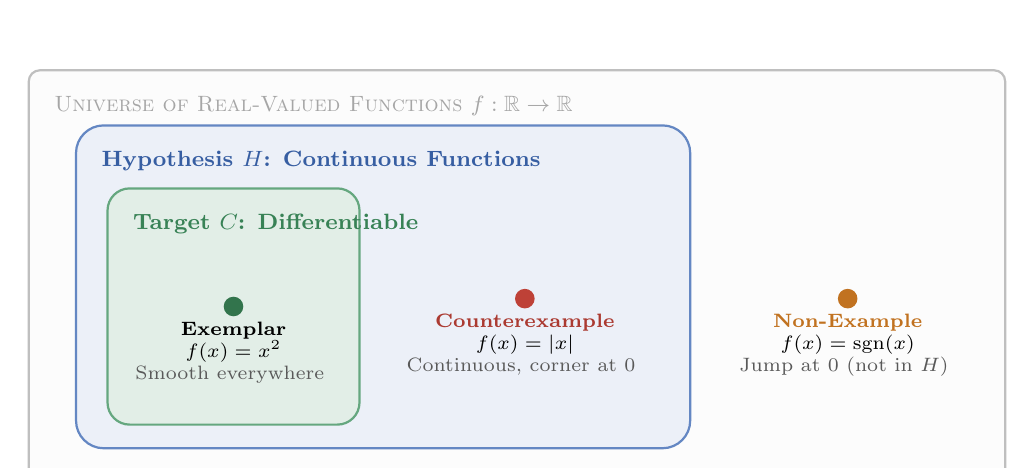
\begin{tikzpicture}[
    font=\small,
    universe/.style={draw=gray!50, fill=gray!2, rounded corners=4pt, thick},
    hypo/.style={draw=sourceblue!80, fill=sourceblue!10, rounded corners=10pt, thick},
    prop/.style={draw=targetgreen!80, fill=targetgreen!15, rounded corners=8pt, thick}
]

\draw[universe] (0, 0) rectangle (12.4, 5.2);
\node[anchor=north west, font=\footnotesize\scshape, text=gray!70] at (0.2, 5.0) {Universe of Real-Valued Functions $f : \R \to \R$};

\draw[hypo] (0.6, 0.4) rectangle (8.4, 4.5);
\node[anchor=north west, font=\footnotesize\bfseries, text=sourceblue!90!black] at (0.8, 4.3) {Hypothesis $H$: Continuous Functions};

\draw[prop] (1.0, 0.7) rectangle (4.2, 3.7);
\node[anchor=north west, font=\footnotesize\bfseries, text=targetgreen!90!black] at (1.2, 3.5) {Target $C$: Differentiable};

\node[circle, fill=targetgreen!80!black, inner sep=2.5pt] (ex) at (2.6, 2.2) {};
\node[below=2pt, font=\scriptsize, align=center] at (ex) {
    \textbf{Exemplar}\\
    $f(x) = x^2$\\
    \color{gray!70!black}Smooth everywhere
};

\node[circle, fill=trapred, inner sep=2.5pt] (cx) at (6.3, 2.3) {};
\node[below=2pt, font=\scriptsize, align=center] at (cx) {
    \textbf{\color{trapred!90!black}Counterexample}\\
    $f(x) = |x|$\\
    \color{gray!70!black}Continuous, corner at $0$
};

\node[circle, fill=quotientorange!90!black, inner sep=2.5pt] (nx) at (10.4, 2.3) {};
\node[below=2pt, font=\scriptsize, align=center] at (nx) {
    \textbf{\color{quotientorange!90!black}Non-Example}\\
    $f(x) = \operatorname{sgn}(x)$\\
    \color{gray!70!black}Jump at $0$ (not in $H$)
};

\end{tikzpicture}
\end{center}

Look closely at the three distinct territories shown in the diagram:
\begin{itemize}
\item \textbf{Standard Exemplars ($f(x) = x^2$)}: Sitting securely inside the target property $C$ (and therefore inside $H$), exemplars confirm that the concept is inhabited. They provide an anchor for geometric intuition.
\item \textbf{Counterexamples ($f(x) = |x|$)}: Sitting inside the hypothesis $H$ (continuous) but outside the target $C$ (differentiable), this single function disproves the universal claim. At $x = 0$, the left-hand slope is $-1$ while the right-hand slope is $+1$, so no tangent line exists. A single function in the difference $H \setminus C$ shows the statement is false.
\item \textbf{Non-examples of the hypothesis ($f(x) = \operatorname{sgn}(x)$)}: The sign function $\operatorname{sgn}(x)$ equals $+1$ for $x > 0$, $-1$ for $x < 0$, and $0$ at the origin. Because it jumps abruptly at $0$, it is not continuous: it sits completely outside $H$. It cannot be used to test whether $H \implies C$, because it never met the entrance condition of the premise.
\end{itemize}

\begin{recoverybox}
\textbf{Pause and think}: Could a function ever sit inside $C$ (differentiable) but outside $H$ (continuous)? No! A core theorem of calculus establishes that if a function is differentiable at $x_0$, then $\lim_{x \to x_0} (f(x) - f(x_0)) = \lim_{x \to x_0} \frac{f(x)-f(x_0)}{x-x_0}(x-x_0) = f'(x_0) \cdot 0 = 0$, which forces $f$ to be continuous at $x_0$. In our geography, the region of differentiable functions outside continuous functions is strictly empty.
\end{recoverybox}

\subsection{The art of the minimal counterexample}

When testing whether a mathematical statement is true, beginners often try to construct elaborate counterexamples. In practice, however, if a statement is false, it often fails on a very simple object.

Consider the claim:
\begin{quote}
``For all real numbers $x$ and $y$, if $x^2 = y^2$, then $x = y$.''
\end{quote}
You do not need a complicated function to test this claim. Testing the simplest signed integers is enough:
\[
x = 1, \quad y = -1 \implies (1)^2 = (-1)^2 = 1, \quad \text{yet } 1 \neq -1.
\]
Testing $x = 1$ and $y = -1$ immediately disproves the claim.

Similarly, consider the statement ``Every prime number is odd.'' The minimal counterexample is the number $2$. It is the only even prime, and serves as an important counterexample in elementary number theory.

\subsubsection*{The danger of trusting early patterns}
Why is a proof required rather than twenty successful examples? Consider Leonhard Euler's famous prime-generating polynomial:
\[
P(n) = n^2 + n + 41.
\]
Let us test the first few whole numbers:
\begin{align*}
n = 0 &\implies P(0) = 41 \quad (\text{prime}), \\
n = 1 &\implies P(1) = 43 \quad (\text{prime}), \\
n = 2 &\implies P(2) = 47 \quad (\text{prime}), \\
n = 3 &\implies P(3) = 53 \quad (\text{prime}).
\end{align*}
If you continue testing by hand, you will find that for every single integer from $n = 0$ all the way to $n = 39$, the polynomial generates a prime number! Forty consecutive successes. In empirical sciences, forty consecutive confirmations with zero failures provide strong inductive evidence.

Yet at $n = 40$, the pattern fails:
\[
P(40) = 40^2 + 40 + 41 = 40(40 + 1) + 41 = 40(41) + 41 = 41(40 + 1) = 41^2 = 1681 = 41 \times 41.
\]
$1681$ is composite. Forty positive cases do not guarantee that the formula always produces primes.

The diagram below visualizes this: forty consecutive tests produce prime numbers, yet the forty-first test disproves the general claim.

\begin{center}
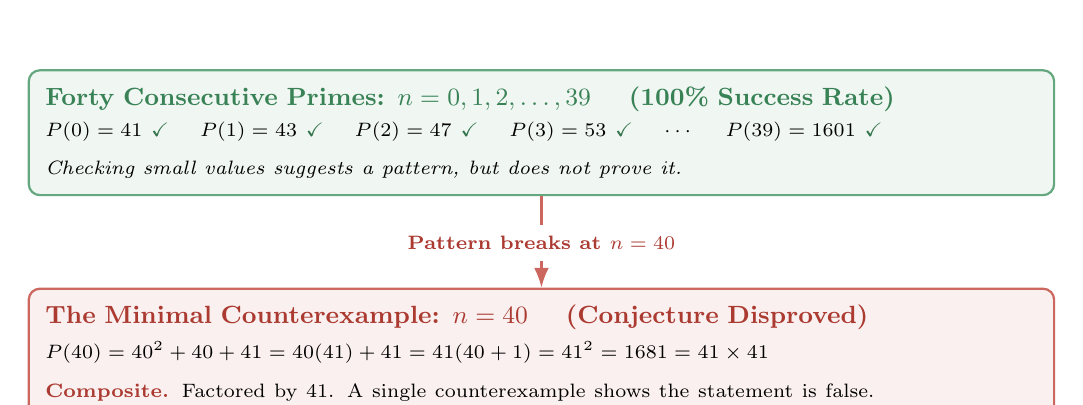
\begin{tikzpicture}[
    font=\small,
    streak/.style={draw=targetgreen!80, fill=targetgreen!8, rounded corners=4pt, thick, text width=12.6cm, inner sep=6pt},
    snap/.style={draw=trapred!80, fill=trapred!8, rounded corners=4pt, thick, text width=12.6cm, inner sep=6pt}
]

% Upper Box: 40 Consecutive Successes
\node[streak] (top) at (6.3, 2.2) {
    \textbf{\color{targetgreen!90!black}Forty Consecutive Primes: $n = 0, 1, 2, \ldots, 39$ \quad (\textbf{100\% Success Rate})}\\[3pt]
    \scriptsize
    $P(0) = 41$ \textbf{\color{targetgreen!80!black}\checkmark} \quad
    $P(1) = 43$ \textbf{\color{targetgreen!80!black}\checkmark} \quad
    $P(2) = 47$ \textbf{\color{targetgreen!80!black}\checkmark} \quad
    $P(3) = 53$ \textbf{\color{targetgreen!80!black}\checkmark} \quad
    $\cdots$ \quad
    $P(39) = 1601$ \textbf{\color{targetgreen!80!black}\checkmark}\\[3pt]
    \emph{Checking small values suggests a pattern, but does not prove it.}
};

% Lower Box: The Sudden Fracture
\node[snap] (bot) at (6.3, -0.6) {
    \textbf{\color{trapred!90!black}The Minimal Counterexample: $n = 40$ \quad (\textbf{Conjecture Disproved})}\\[3pt]
    \scriptsize
    $P(40) = 40^2 + 40 + 41 = 40(41) + 41 = 41(40 + 1) = 41^2 = 1681 = 41 \times 41$\\[3pt]
    \textbf{\color{trapred!90!black}Composite.} Factored by $41$. A single counterexample shows the statement is false.
};

% Connecting Label and Arrows
\node[font=\scriptsize\bfseries, text=trapred!90!black, inner sep=4pt] (mid) at (6.3, 0.8) {Pattern breaks at $n=40$};
\draw[thick, trapred!80] (top.south) -- (mid.north);
\draw[-{Latex[length=2.5mm]}, thick, trapred!80] (mid.south) -- (bot.north);

\end{tikzpicture}
\end{center}

\subsubsection*{Common test cases}
When testing a conjecture, standard test cases often expose false statements quickly:
\begin{itemize}
\item \textbf{Numbers}: $0$ (which flattens products to zero), $1$ and $-1$ (which preserve squares while flipping signs), negative numbers (which reverse inequalities when multiplied), fractions strictly between $0$ and $1$ (where powers shrink rather than grow: $(1/2)^2 = 1/4 < 1/2$), and irrational numbers like $\sqrt{2}$ (numbers that cannot be written as a fraction of integers).
\item \textbf{Sets}: the empty set $\emptyset$ (the set containing no elements, which often satisfies conditional statements vacuously), singletons $\{a\}$ (sets with exactly one member), and disjoint sets (sets that share no elements).
\item \textbf{Functions}: the constant zero function $f(x) = 0$, the identity function $f(x) = x$, absolute value $f(x) = |x|$ (which introduces a sharp corner), step functions (which have jump discontinuities), and the reciprocal $f(x) = 1/x$ (which shoots to infinity at zero).
\item \textbf{Matrices}: the zero matrix $O$, the identity matrix $I$, projection matrices (matrices satisfying $P^2 = P$, which flatten space onto a subspace), and nilpotent matrices (non-zero matrices that square to zero, such as $N = \begin{pmatrix} 0 & 1 \\ 0 & 0 \end{pmatrix}$, where $N^2 = \begin{pmatrix} 0 & 0 \\ 0 & 0 \end{pmatrix}$).
\end{itemize}

\subsection{Stress-testing theorems: removing assumptions}

A useful practice for understanding theorems is to remove one hypothesis and construct an object showing why the theorem then fails. Each hypothesis in a theorem is necessary for the conclusion to hold.

Consider the \textbf{Extreme Value Theorem}:
\begin{theorem}[Extreme Value Theorem]
Let $f : [a, b] \to \R$ be a continuous function on a closed and bounded interval. Then $f$ attains both an absolute maximum and an absolute minimum.
\end{theorem}

Before manipulating this statement, unpack the vocabulary:
\begin{itemize}
\item A \textbf{closed interval} $[a, b]$ is one that includes both of its boundary endpoints $a$ and $b$.
\item A \textbf{bounded interval} is one that has finite length, rather than stretching off to infinity.
\item A function \textbf{attains an absolute maximum} if there is an actual point $c \in [a, b]$ where $f(c) \ge f(x)$ for all $x \in [a, b]$---meaning the function takes on its maximum value at some point in the domain, rather than merely approaching an upper bound.
\end{itemize}

Notice the three distinct hypotheses: (1) closed interval, (2) bounded interval, (3) continuous function. What happens if you drop each requirement one by one?

\begin{enumerate}
\item \textbf{Drop ``closed''}: Replace $[0, 1]$ with the open interval $(0, 1)$ and choose the simple identity function $f(x) = x$. As $x$ approaches $1$ from the left, the outputs get arbitrarily close to $1$. But $1 \notin (0, 1)$. For any point $x \in (0, 1)$, the midpoint $\frac{x+1}{2}$ is also in $(0, 1)$ and gives a strictly higher value. The ceiling $1$ is the \textbf{supremum} (the least upper bound), but it is not attained by any input in $(0, 1)$. The function has no maximum value!
\item \textbf{Drop ``bounded''}: Replace $[0, 1]$ with the unbounded ray $[0, \infty)$ and keep $f(x) = x$. The function grows without bound and attains no maximum.
\item \textbf{Drop ``continuous''}: Keep the closed and bounded domain $[0, 1]$, but introduce a single jump discontinuity at the right boundary:
\[
f(x) = \begin{cases} x & \text{if } 0 \le x < 1, \\ 0 & \text{if } x = 1. \end{cases}
\]
On $[0, 1)$, the values climb steadily toward $1$. But at the very moment $x$ reaches $1$, the output plunges to $0$. The supremum $1$ is not attained.
\end{enumerate}

\begin{center}
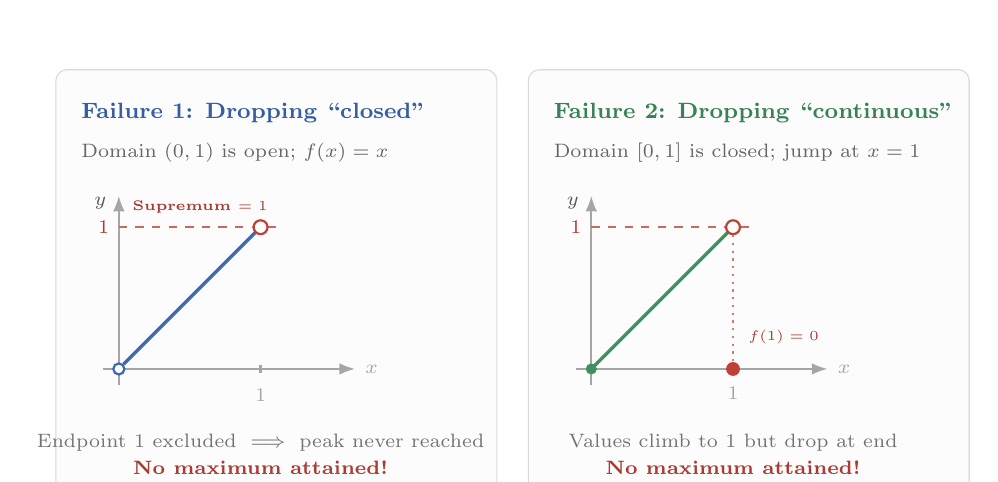
\begin{tikzpicture}[font=\small]

% Panel 1: Dropping "closed"
\begin{scope}[xshift=0cm]
    \draw[draw=gray!30, fill=gray!2, rounded corners=4pt] (-0.8, -1.6) rectangle (4.8, 3.8);
    \node[anchor=north west, font=\footnotesize\bfseries, text=sourceblue!90!black] at (-0.6, 3.5) {Failure 1: Dropping ``closed''};
    \node[anchor=north west, font=\scriptsize, text=gray!80!black] at (-0.6, 3.0) {Domain $(0, 1)$ is open; $f(x) = x$};

    \draw[-{Latex[length=2mm]}, thick, gray!70] (-0.2, 0) -- (3.0, 0) node[right, font=\scriptsize] {$x$};
    \draw[-{Latex[length=2mm]}, thick, gray!70] (0, -0.2) -- (0, 2.2);
    \node[left=1pt, font=\scriptsize, text=gray!70!black] at (0, 2.1) {$y$};

    \draw[dashed, trapred!80, thick] (0, 1.8) -- (2.0, 1.8);
    \node[left, font=\scriptsize, text=trapred!90!black] at (0, 1.8) {$1$};
    \node[anchor=south west, font=\tiny\bfseries, text=trapred!90!black] at (0.05, 1.85) {Supremum $= 1$};

    \draw[very thick, sourceblue] (0.06, 0.06) -- (1.74, 1.74);
    \draw[thick, sourceblue, fill=white] (0, 0) circle (2pt);
    \draw[thick, trapred, fill=white] (1.8, 1.8) circle (2.5pt);

    \draw[thick, gray!70] (1.8, 1.5pt) -- (1.8, -1.5pt) node[below=2pt, font=\scriptsize] {$1$};

    \node[below, font=\scriptsize, text=gray!90!black, align=center] at (1.8, -0.7) {
        Endpoint $1$ excluded $\implies$ peak never reached\\[2pt]
        \textbf{\color{trapred!90!black}No maximum attained!}
    };
\end{scope}

% Panel 2: Dropping "continuous"
\begin{scope}[xshift=6.0cm]
    \draw[draw=gray!30, fill=gray!2, rounded corners=4pt] (-0.8, -1.6) rectangle (4.8, 3.8);
    \node[anchor=north west, font=\footnotesize\bfseries, text=targetgreen!90!black] at (-0.6, 3.5) {Failure 2: Dropping ``continuous''};
    \node[anchor=north west, font=\scriptsize, text=gray!80!black] at (-0.6, 3.0) {Domain $[0, 1]$ is closed; jump at $x = 1$};

    \draw[-{Latex[length=2mm]}, thick, gray!70] (-0.2, 0) -- (3.0, 0) node[right, font=\scriptsize] {$x$};
    \draw[-{Latex[length=2mm]}, thick, gray!70] (0, -0.2) -- (0, 2.2);
    \node[left=1pt, font=\scriptsize, text=gray!70!black] at (0, 2.1) {$y$};

    \draw[dashed, trapred!80, thick] (0, 1.8) -- (2.0, 1.8);
    \node[left, font=\scriptsize, text=trapred!90!black] at (0, 1.8) {$1$};

    \draw[very thick, targetgreen] (0, 0) -- (1.74, 1.74);
    \fill[targetgreen] (0, 0) circle (2pt);
    \draw[thick, trapred, fill=white] (1.8, 1.8) circle (2.5pt);

    \draw[dotted, thick, trapred!70] (1.8, 1.7) -- (1.8, 0.1);
    \fill[trapred] (1.8, 0) circle (2.5pt);
    \node[right=2pt, font=\tiny\bfseries, text=trapred!90!black] at (1.8, 0.4) {$f(1) = 0$};

    \node[below=3pt, font=\scriptsize, text=gray!70] at (1.8, 0) {$1$};

    \node[below, font=\scriptsize, text=gray!90!black, align=center] at (1.8, -0.7) {
        Values climb to $1$ but drop at end\\[2pt]
        \textbf{\color{trapred!90!black}No maximum attained!}
    };
\end{scope}

\end{tikzpicture}
\end{center}

Each hypothesis was necessary: removing any one of them allows the conclusion to fail.

\begin{historybox}
In 1752, Leonhard Euler announced a geometric law: for any \textbf{polyhedron}---a solid three-dimensional shape with flat polygonal faces, straight edges, and sharp corner vertices, such as a cube or pyramid---the number of vertices ($V$), edges ($E$), and faces ($F$) satisfies:
\[
V - E + F = 2.
\]
For a cube, $8 - 12 + 6 = 2$; for a tetrahedron, $4 - 6 + 4 = 2$. In 1813, Augustin-Louis Cauchy published what appeared to be an airtight proof by removing one face and flattening the remaining network of edges onto a flat two-dimensional plane.

Yet over the following century, unexpected geometric ``monsters'' appeared. Johannes Kepler had already described self-intersecting star polyhedra (solids whose faces pass through one another), which yield $12 - 30 + 12 = -6$. In 1813, the Swiss mathematician Louis Lhuilier demonstrated that a picture-frame polyhedron with a central square tunnel gives $V - E + F = 0$, while a hollow cube floating inside another cube gives $V - E + F = 4$.

In his 1976 masterwork \emph{Proofs and Refutations}, the philosopher Imre Lakatos analyzed this history to show that mathematical discovery does not proceed in a straight line from unquestioned axioms to permanent theorems. Instead, it advances through a living dialogue of bold conjectures and surprising counterexamples. Early mathematicians reacted with ``monster-barring''---declaring that solids with tunnels or self-intersections were ``not real polyhedra'' to defend Euler's original equation. The true breakthrough came from inspecting where Cauchy's proof had quietly made an unstated assumption: Cauchy had assumed that every polyhedron could be inflated like a balloon into a round sphere.

By incorporating the missing topological condition---the \textbf{genus} $g$, which counts the number of donut-like tunnels passing through the solid---mathematicians established the universal formula:
\[
V - E + F = 2 - 2g.
\]
This quantity is the simplest example of a \textbf{topological invariant}: a numerical quantity that does not change when a shape is continuously stretched, bent, or compressed without tearing. Counterexamples led directly to the formulation of modern topological invariants.
\end{historybox}

The diagram below shows how a geometric counterexample reshapes a naive theorem: Lhuilier's tunnel polyhedron breaks Euler's original $V - E + F = 2$, revealing the hidden topological invariant $g$.

\begin{center}
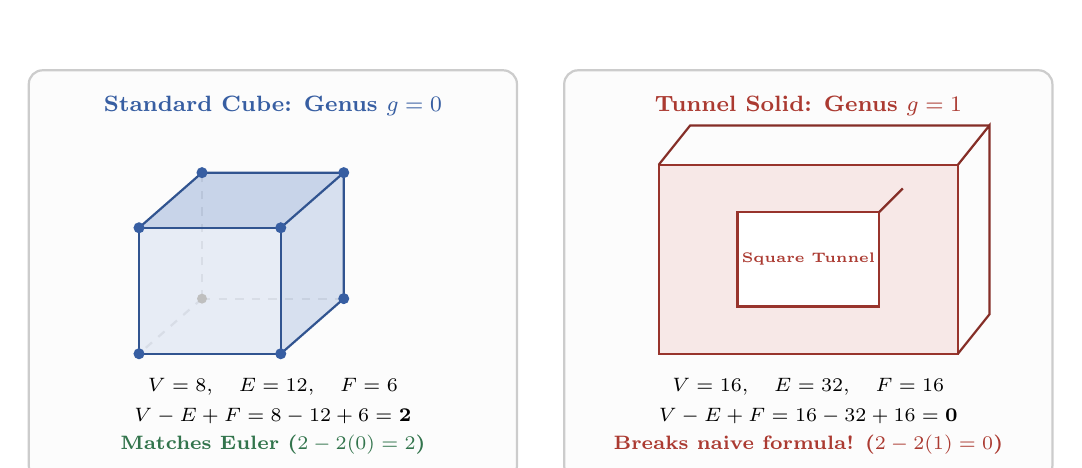
\begin{tikzpicture}[
    font=\small,
    panel/.style={draw=gray!40, fill=gray!2, rounded corners=5pt, thick, inner sep=6pt}
]

% Panel 1: Convex Polyhedron (Cube, g=0)
\begin{scope}[xshift=0cm]
    \node[panel, minimum width=6.2cm, minimum height=5.2cm] (p1) at (2.6, 1.8) {};
    \node[anchor=north, font=\footnotesize\bfseries, text=sourceblue!90!black] at (2.6, 4.2) {Standard Cube: Genus $g = 0$};

    % Cube 3D drawing
    % Back hidden lines
    \draw[dashed, gray!60, thick] (1.7, 1.5) -- (3.5, 1.5);
    \draw[dashed, gray!60, thick] (1.7, 1.5) -- (1.7, 3.1);
    \draw[dashed, gray!60, thick] (1.7, 1.5) -- (0.9, 0.8);

    % Faces shading
    \fill[sourceblue!15, opacity=0.8] (0.9, 0.8) -- (2.7, 0.8) -- (2.7, 2.4) -- (0.9, 2.4) -- cycle;
    \fill[sourceblue!25, opacity=0.8] (2.7, 0.8) -- (3.5, 1.5) -- (3.5, 3.1) -- (2.7, 2.4) -- cycle;
    \fill[sourceblue!35, opacity=0.8] (0.9, 2.4) -- (2.7, 2.4) -- (3.5, 3.1) -- (1.7, 3.1) -- cycle;

    % Visible edges
    \draw[thick, sourceblue!80!black] (0.9, 0.8) -- (2.7, 0.8) -- (2.7, 2.4) -- (0.9, 2.4) -- cycle;
    \draw[thick, sourceblue!80!black] (2.7, 0.8) -- (3.5, 1.5) -- (3.5, 3.1) -- (2.7, 2.4);
    \draw[thick, sourceblue!80!black] (0.9, 2.4) -- (1.7, 3.1) -- (3.5, 3.1);

    % Vertices dots
    \foreach \coord in {(0.9,0.8), (2.7,0.8), (2.7,2.4), (0.9,2.4), (3.5,1.5), (3.5,3.1), (1.7,3.1)} {
        \fill[sourceblue!90!black] \coord circle (2pt);
    }
    \fill[gray!50] (1.7, 1.5) circle (1.8pt);

    \node[anchor=south, font=\scriptsize, align=center] at (2.6, -0.6) {
        $V = 8, \quad E = 12, \quad F = 6$\\[3pt]
        $V - E + F = 8 - 12 + 6 = \mathbf{2}$\\[2pt]
        \textbf{\color{targetgreen!80!black}Matches Euler ($2 - 2(0) = 2$)}
    };
\end{scope}

% Panel 2: Tunnel Polyhedron (Picture frame, g=1)
\begin{scope}[xshift=6.8cm]
    \node[panel, minimum width=6.2cm, minimum height=5.2cm] (p2) at (2.6, 1.8) {};
    \node[anchor=north, font=\footnotesize\bfseries, text=trapred!90!black] at (2.6, 4.2) {Tunnel Solid: Genus $g = 1$};

    % Schematic frame representation
    % Outer block
    \draw[thick, trapred!80!black, fill=trapred!12] (0.7, 0.8) rectangle (4.5, 3.2);
    % Inner tunnel
    \draw[thick, trapred!80!black, fill=white] (1.7, 1.4) rectangle (3.5, 2.6);
    \node[font=\tiny\bfseries, text=trapred!90!black] at (2.6, 2.0) {Square Tunnel};

    % 3D frame depth lines
    \draw[thick, trapred!70!black] (4.5, 0.8) -- (4.9, 1.3) -- (4.9, 3.7) -- (4.5, 3.2);
    \draw[thick, trapred!70!black] (4.9, 3.7) -- (1.1, 3.7) -- (0.7, 3.2);
    \draw[thick, trapred!70!black] (3.5, 2.6) -- (3.8, 2.9);

    \node[anchor=south, font=\scriptsize, align=center] at (2.6, -0.6) {
        $V = 16, \quad E = 32, \quad F = 16$\\[3pt]
        $V - E + F = 16 - 32 + 16 = \mathbf{0}$\\[2pt]
        \textbf{\color{trapred!90!black}Breaks naive formula! ($2 - 2(1) = 0$)}
    };
\end{scope}

\end{tikzpicture}
\end{center}

\subsection{Why set theory provides the shared framework}

Seeking exemplars, non-examples, and counterexamples grounds abstract statements in concrete behavior. By testing extreme cases ($0, 1, -1, \emptyset$) and removing hypotheses one by one, you discover why each condition in a theorem is needed.

Testing statements across numbers, functions, and shapes raises a natural question: what common language connects these different kinds of mathematical objects? In Chapter~10 (\emph{Sets: The Grammar of Modern Mathematics}), we introduce set theory, the framework used throughout modern mathematics to define and organize objects.

\subsection{Exercises}

\paragraph{Quick mental checks.} For each statement below, find a counterexample:
\begin{enumerate}
\item For all real numbers $a$ and $b$, if $ab = 0$, then $a = 0$ and $b = 0$.
\item For every real number $x$, if $x^2 > 4$, then $x > 2$.
\item If a polygon in the plane has four equal sides, it must be a square.
\item For all positive integers $a, b, c$, if $a$ divides the product $bc$, then $a$ divides $b$ or $a$ divides $c$.
\end{enumerate}

\paragraph{Routine practice.} Provide a concrete counterexample for each false claim and identify precisely which condition or hypothesis fails:
\begin{enumerate}[resume]
\item For all sets $A, B, C$, if $A \cup B = A \cup C$, then $B = C$.
\item For all sets $A, B, C$, if $A \cap B = A \cap C$, then $B = C$.
\item If a differentiable function $f : D \to \R$ satisfies $f'(x) = 0$ for every $x \in D$, then $f$ is a constant function. (Hint: What if the domain $D$ consists of two disconnected pieces, such as $(-\infty, 0) \cup (0, \infty)$?)
\item Every sequence of rational numbers that converges in $\R$ must have a rational limit. (Hint: Consider decimal truncations of an irrational number, such as $1, 1.4, 1.41, 1.414, \ldots \to \sqrt{2}$.)
\item For all real numbers $x$, if $x^2 \ge x$, then $x \ge 1$.
\end{enumerate}

\paragraph{Deeper exploration.}
\begin{enumerate}[resume]
\item \textbf{Euler's sum-of-powers conjecture}: In 1769, Leonhard Euler conjectured that for all integers $n > 2$, it requires at least $n$ positive $n$-th powers to sum to another $n$-th power. For $n = 3$, this asserts that two cubes cannot sum to a cube (the $n=3$ case of Fermat's Last Theorem), requiring three cubes ($3^3 + 4^3 + 5^3 = 6^3$). For $n = 5$, Euler's conjecture claimed that no four fifth powers could sum to a fifth power: $a^5 + b^5 + c^5 + d^5 = e^5$ was conjectured to be impossible. In 1966, L.~J.~Lander and T.~R.~Parkin discovered the following equality:
\[
27^5 + 84^5 + 110^5 + 133^5 = 144^5.
\]
Verify by direct calculation that this identity holds. Explain why this single numerical counterexample permanently settled a conjecture that had stood for 197 years.
\item \textbf{Patterns and proof}: In 1650, Pierre de Fermat inspected the numbers $F_n = 2^{2^n} + 1$:
\[
F_0 = 3, \quad F_1 = 5, \quad F_2 = 17, \quad F_3 = 257, \quad F_4 = 65537.
\]
Observing that all five numbers are prime, Fermat conjectured that $F_n$ is prime for every non-negative integer $n$. In 1732, Leonhard Euler factored the very next term:
\[
F_5 = 2^{32} + 1 = 4{,}294{,}967{,}297 = 641 \times 6{,}700{,}417.
\]
Explain the philosophical difference between scientific induction (generalizing from observed instances) and mathematical proof: why can no finite collection of examples ever prove a statement of the form $\forall n \in \N, \, P(n)$?
\end{enumerate}

\newpage

\section{Sets: The Grammar of Modern Mathematics}
\chapterline

In elementary mathematics, arithmetic operates on numbers, algebra operates on equations, and calculus operates on functions. But when you ask what numbers, equations, and functions actually \emph{are}, modern mathematics answers in a single unified vocabulary: they are all built from \textbf{sets}.

A set is a well-defined collection of distinct objects. The objects belonging to a set are called its \textbf{elements} (or members). We write:
\begin{align*}
x \in A &\quad \text{to assert that } x \text{ is an element of } A, \\
x \notin A &\quad \text{to assert that } x \text{ is not an element of } A.
\end{align*}

This foundation seems deceptively simple. Yet sets serve as the universal scaffolding for advanced mathematics: spaces are sets of points equipped with distance or topology; groups are sets equipped with lawful operations; relations are sets of ordered pairs; and differential equations are conditions selecting subsets of function spaces.

\begin{historybox}
In the 1870s, the German mathematician Georg Cantor invented set theory while studying which collections of numbers allow a trigonometric wave to be uniquely reconstructed. Cantor realized that to tame infinity, mathematics needed a language that could treat infinite collections as completed objects in their own right. He showed that sets could serve as the universal atom out of which numbers, functions, and geometric spaces are built.

At the turn of the twentieth century, Gottlob Frege attempted to ground all of arithmetic and mathematics in this new foundation in his monumental \emph{Grundgesetze der Arithmetik}. Frege relied on what seemed like an obvious truth: \emph{Unrestricted Comprehension}---the belief that any mathematical condition you can write down creates a valid set of all objects satisfying it. But in June 1902, the British philosopher Bertrand Russell sent Frege a brief letter that shattered naive set theory. Russell asked: what happens if you consider the set of all sets that do not contain themselves?
\[
R = \{x : x \notin x\}.
\]
If $R$ is not an element of itself, it meets the entrance criteria, so it must belong to $R$. But if $R$ does belong to $R$, it fails the condition, so it cannot belong to $R$! The foundation of logic had generated an inescapable contradiction. Frege wrote in an appendix that a scientist can hardly meet with anything more undesirable than having their foundation collapse just as the work is finished.

Mathematicians led by Ernst Zermelo (1908) and Adolf Fraenkel (1922) repaired the foundation by replacing naive set theory with modern axiomatic set theory (ZFC). Under the new rules, you can only carve out subsets from an \emph{already existing} set ($\{x \in A : P(x)\}$), banishing self-referential monsters and the dangerous ``set of all sets.'' Sets became the bedrock of modern mathematics.
\end{historybox}

\subsection{The crucial distinction: element versus subset}

The single most common source of early confusion is conflating \textbf{membership} ($\in$) with \textbf{containment} ($\subseteq$).

\begin{itemize}
\item \textbf{Membership ($x \in A$)}: A relation between an individual object and a container. $x$ is one of the items sitting inside the box $A$.
\item \textbf{Subset ($A \subseteq B$)}: A relation between two containers. $A \subseteq B$ means that \emph{every} element of $A$ is also an element of $B$:
\[
A \subseteq B \iff \forall x, \, (x \in A \implies x \in B).
\]
\end{itemize}

To see how easy it is to trip if you are not careful, consider the set:
\[
S = \bigl\{1, \, 2, \, \{3, 4\}\bigr\}.
\]
Notice that $S$ contains exactly \emph{three} elements: the number $1$, the number $2$, and the package $\{3, 4\}$.
\begin{itemize}
\item $1 \in S$ is \textbf{True}.
\item $\{1\} \subseteq S$ is \textbf{True} (because $1 \in S$).
\item $\{1\} \in S$ is \textbf{False} (the number $1$ is inside $S$, but the set $\{1\}$ is not).
\item $\{3, 4\} \in S$ is \textbf{True} (the package $\{3, 4\}$ is literally an element of $S$).
\item $\{3, 4\} \subseteq S$ is \textbf{False} (because $3 \notin S$ and $4 \notin S$; the elements $3$ and $4$ are trapped inside the inner box).
\item $\bigl\{\{3, 4\}\bigr\} \subseteq S$ is \textbf{True} (a set containing the element $\{3, 4\}$).
\end{itemize}

Think of a box containing an apple, an orange, and a sealed envelope with two photographs inside. The apple is an element of the box. The envelope is an element of the box. But the photographs are \emph{not} loose elements of the box; they are elements of the envelope!

\subsection{The four fundamental set operations}

Given two sets $A$ and $B$ living inside a universal set $U$, we can combine and filter them using four primary operations:

\begin{center}
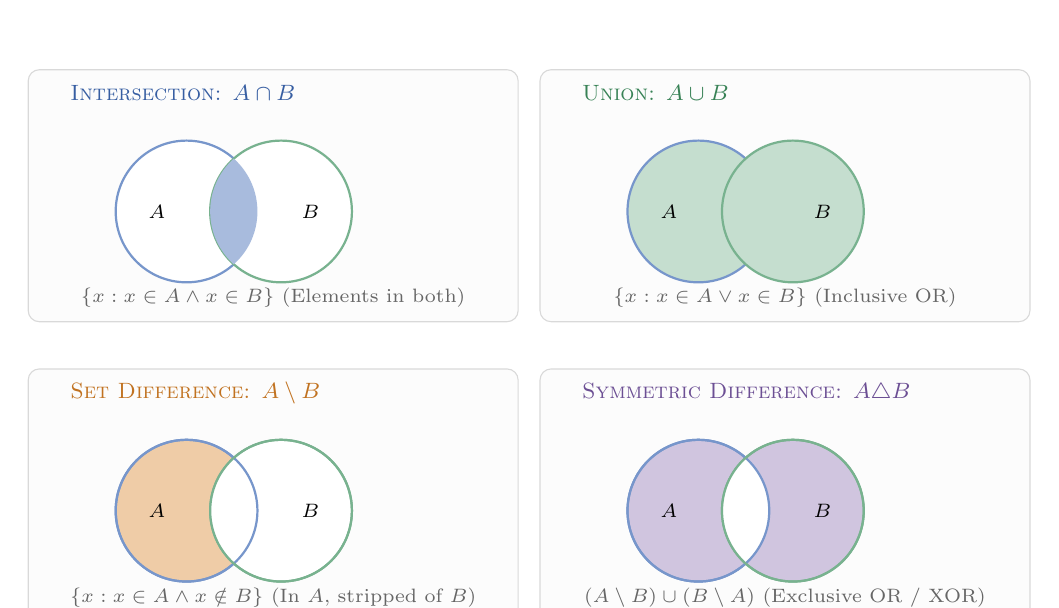
\begin{tikzpicture}[
    font=\small,
    subpanel/.style={draw=gray!30, fill=gray!2, rounded corners=4pt, inner sep=6pt}
]

% Panel 1: Intersection (Top Left)
\node[subpanel, text width=5.8cm, minimum height=3.2cm] (p1) at (0, 3.8) {};
\node[anchor=west, font=\footnotesize\scshape, text=sourceblue!90!black] at (-2.7, 5.1) {Intersection: $A \cap B$};
\begin{scope}[xshift=-0.5cm, yshift=3.6cm, scale=0.75]
    \draw[thick, draw=sourceblue!70, fill=white] (-0.8, 0) circle (1.2);
    \draw[thick, draw=targetgreen!70, fill=white] (0.8, 0) circle (1.2);
    \begin{scope}
        \clip (-0.8, 0) circle (1.2);
        \fill[sourceblue!45] (0.8, 0) circle (1.2);
    \end{scope}
    \node[font=\scriptsize] at (-1.3, 0) {$A$};
    \node[font=\scriptsize] at (1.3, 0) {$B$};
\end{scope}
\node[font=\scriptsize, text=gray!80!black] at (0, 2.5) {$\{x : x \in A \land x \in B\}$ (Elements in both)};

% Panel 2: Union (Top Right)
\node[subpanel, text width=5.8cm, minimum height=3.2cm] (p2) at (6.5, 3.8) {};
\node[anchor=west, font=\footnotesize\scshape, text=targetgreen!90!black] at (3.8, 5.1) {Union: $A \cup B$};
\begin{scope}[xshift=6.0cm, yshift=3.6cm, scale=0.75]
    \draw[thick, draw=sourceblue!70, fill=targetgreen!30] (-0.8, 0) circle (1.2);
    \draw[thick, draw=targetgreen!70, fill=targetgreen!30] (0.8, 0) circle (1.2);
    \node[font=\scriptsize] at (-1.3, 0) {$A$};
    \node[font=\scriptsize] at (1.3, 0) {$B$};
\end{scope}
\node[font=\scriptsize, text=gray!80!black] at (6.5, 2.5) {$\{x : x \in A \lor x \in B\}$ (Inclusive OR)};

% Panel 3: Set Difference (Bottom Left)
\node[subpanel, text width=5.8cm, minimum height=3.2cm] (p3) at (0, 0) {};
\node[anchor=west, font=\footnotesize\scshape, text=quotientorange!90!black] at (-2.7, 1.3) {Set Difference: $A \setminus B$};
\begin{scope}[xshift=-0.5cm, yshift=-0.2cm, scale=0.75]
    \draw[thick, draw=sourceblue!70, fill=quotientorange!40] (-0.8, 0) circle (1.2);
    \draw[thick, draw=targetgreen!70, fill=white] (0.8, 0) circle (1.2);
    \begin{scope}
        \clip (0.8, 0) circle (1.2);
        \fill[white] (-0.8, 0) circle (1.2);
    \end{scope}
    \draw[thick, draw=sourceblue!70] (-0.8, 0) circle (1.2);
    \draw[thick, draw=targetgreen!70] (0.8, 0) circle (1.2);
    \node[font=\scriptsize] at (-1.3, 0) {$A$};
    \node[font=\scriptsize] at (1.3, 0) {$B$};
\end{scope}
\node[font=\scriptsize, text=gray!80!black] at (0, -1.3) {$\{x : x \in A \land x \notin B\}$ (In $A$, stripped of $B$)};

% Panel 4: Symmetric Difference (Bottom Right)
\node[subpanel, text width=5.8cm, minimum height=3.2cm] (p4) at (6.5, 0) {};
\node[anchor=west, font=\footnotesize\scshape, text=structurepurple!90!black] at (3.8, 1.3) {Symmetric Difference: $A \triangle B$};
\begin{scope}[xshift=6.0cm, yshift=-0.2cm, scale=0.75]
    \draw[thick, draw=sourceblue!70, fill=structurepurple!35] (-0.8, 0) circle (1.2);
    \draw[thick, draw=targetgreen!70, fill=structurepurple!35] (0.8, 0) circle (1.2);
    \begin{scope}
        \clip (-0.8, 0) circle (1.2);
        \fill[white] (0.8, 0) circle (1.2);
    \end{scope}
    \draw[thick, draw=sourceblue!70] (-0.8, 0) circle (1.2);
    \draw[thick, draw=targetgreen!70] (0.8, 0) circle (1.2);
    \node[font=\scriptsize] at (-1.3, 0) {$A$};
    \node[font=\scriptsize] at (1.3, 0) {$B$};
\end{scope}
\node[font=\scriptsize, text=gray!80!black] at (6.5, -1.3) {$(A \setminus B) \cup (B \setminus A)$ (Exclusive OR / XOR)};

\end{tikzpicture}
\end{center}

\subsection{Cartesian products: building multidimensional worlds}

When we want to pair elements together in a specific sequence, set membership alone is insufficient because sets are unordered ($\{1, 2\} = \{2, 1\}$). To introduce order, mathematics defines the \textbf{ordered pair} $(a, b)$, where order matters: $(1, 2) \neq (2, 1)$.

\begin{definition}
The \emph{Cartesian product} of two sets $A$ and $B$, denoted $A \times B$, is the set of all ordered pairs whose first coordinate comes from $A$ and second coordinate comes from $B$:
\[
A \times B = \{(a, b) : a \in A \text{ and } b \in B\}.
\]
\end{definition}

If $A = \{1, 2, 3, 4\}$ and $B = \{u, v, w\}$, the Cartesian product $A \times B$ forms a discrete $4 \times 3$ coordinate grid:

\begin{center}
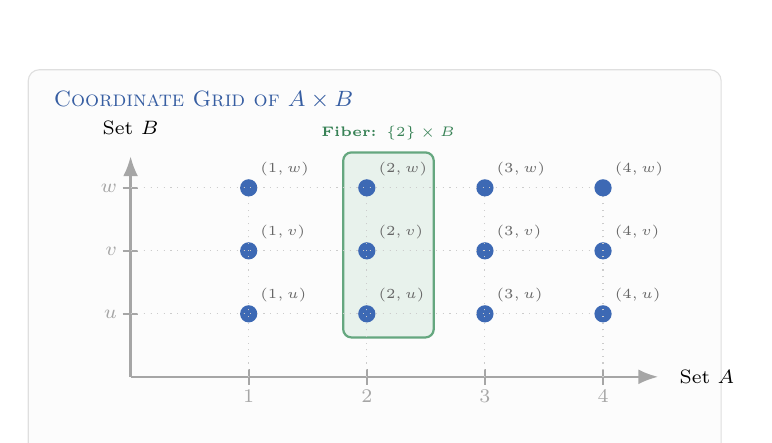
\begin{tikzpicture}[
    font=\small,
    axis/.style={draw=gray!70, -{Latex[length=2.5mm]}, thick},
    gridpt/.style={circle, fill=sourceblue, inner sep=2.2pt}
]

% Background grid panel
\draw[draw=gray!25, fill=gray!2, rounded corners=4pt] (-0.8, -0.6) rectangle (8.0, 4.3);
\node[anchor=north west, font=\footnotesize\scshape, text=sourceblue!90!black] at (-0.6, 4.15) {Coordinate Grid of $A \times B$};

% Coordinate axes
\draw[axis] (0.5, 0.4) -- (7.2, 0.4) node[right=4pt, font=\scriptsize] {Set $A$};
\draw[axis] (0.5, 0.4) -- (0.5, 3.2) node[above=4pt, font=\scriptsize] {Set $B$};

% Ticks on A
\foreach \x/\label in {2.0/1, 3.5/2, 5.0/3, 6.5/4} {
    \draw[thick, gray!70] (\x, 0.3) -- (\x, 0.5) node[below=4pt, font=\scriptsize\bfseries] {$\label$};
}

% Ticks on B
\foreach \y/\label in {1.2/u, 2.0/v, 2.8/w} {
    \draw[thick, gray!70] (0.4, \y) -- (0.6, \y) node[left=4pt, font=\scriptsize\bfseries] {$\label$};
}

% Highlighted slice: {2} x B (drawn behind grid points so labels stay crisp)
\draw[draw=targetgreen!80, fill=targetgreen!12, rounded corners=3pt, thick] (3.2, 0.9) rectangle (4.35, 3.25);
\node[font=\tiny\bfseries, text=targetgreen!90!black, align=center] at (3.77, 3.5) {Fiber: $\{2\} \times B$};

% Grid points
\foreach \x/\lx in {2.0/1, 3.5/2, 5.0/3, 6.5/4} {
    \foreach \y/\ly in {1.2/u, 2.0/v, 2.8/w} {
        \draw[dotted, gray!40] (\x, 0.4) -- (\x, 2.8);
        \draw[dotted, gray!40] (0.5, \y) -- (6.5, \y);
        \node[gridpt] at (\x, \y) {};
        \node[above right=1pt, font=\tiny, text=gray!80!black] at (\x, \y) {$(\lx, \ly)$};
    }
}

\end{tikzpicture}
\end{center}

When both sets are the real line $\R$, the Cartesian product $\R \times \R = \R^2$ is the familiar Euclidean plane. Every point in coordinate geometry is simply an element of a Cartesian product!

\subsection{Proving set equality: double containment}

How do you prove that two set expressions describe the exact same set, such as $A \cap (B \cup C) = (A \cap B) \cup (A \cap C)$?

You cannot merely draw a Venn diagram and declare it finished. A formal proof of $S = T$ requires establishing \textbf{mutual containment} in two separate phases:
\begin{enumerate}
\item \textbf{Show $S \subseteq T$}: Let $x \in S$ be arbitrary. Trace $x$ through the definitions until you deduce $x \in T$.
\item \textbf{Show $T \subseteq S$}: Let $x \in T$ be arbitrary. Trace $x$ through the definitions until you deduce $x \in S$.
\end{enumerate}

\begin{theorem}
For any sets $A$ and $B$, $A \cap B = A \setminus (A \setminus B)$.
\end{theorem}

\begin{proof}
We prove both inclusions:

\textbf{Direction 1: Show $A \cap B \subseteq A \setminus (A \setminus B)$.}
Let $x \in A \cap B$ be arbitrary. By definition of intersection, $x \in A$ and $x \in B$.
Now examine the set $A \setminus B = \{y : y \in A \land y \notin B\}$. Since $x \in B$, $x$ cannot satisfy the condition $x \notin B$. Thus, $x \notin (A \setminus B)$.
Since we know $x \in A$ and $x \notin (A \setminus B)$, by definition of set difference we have $x \in A \setminus (A \setminus B)$. This establishes the first inclusion.

\textbf{Direction 2: Show $A \setminus (A \setminus B) \subseteq A \cap B$.}
Let $x \in A \setminus (A \setminus B)$ be arbitrary. By definition of set difference, $x \in A$ and $x \notin (A \setminus B)$.
Recall that $A \setminus B$ is the set of elements in $A$ that are not in $B$. Since $x \in A$, the only way for $x$ to fail to belong to $A \setminus B$ is if $x \in B$.
Since $x \in A$ and $x \in B$, by definition of intersection we have $x \in A \cap B$. This establishes the second inclusion.

Having established both containments, we conclude that $A \cap B = A \setminus (A \setminus B)$.
\end{proof}

\subsection{What set grammar unlocked---and the need for dynamic maps}

Set theory unlocked a universal language for the mathematical sciences. Concepts from disparate fields---vectors in physics, events in probability, algorithms in computer science, and geometric surfaces in calculus---are all formalized in the single unified language of sets, membership, subsets, and Cartesian coordinate grids. Proving mutual containment through element chasing provides an unshakeable algorithmic technique for establishing that two complex mathematical structures are identical.

Yet sets alone have an honest limitation: \textbf{they are purely static collections}. A set tells you which elements live inside its borders, but it does not describe motion, transformation, or structural relationships between different worlds. How do you map a point from the Euclidean plane into a curved sphere? How do you transform a vector without tearing space? 

To breathe dynamic life into static collections, we need structured mappings. In Chapter~11 (\emph{Set Proofs: Element Chasing in Detail}), we master the fine art of element-chasing proofs, and in Chapter~12 (\emph{Functions: Structured Promises, Not Just Formulas}), we build the modern theory of functions that connect sets across the mathematical universe.

\subsection{Exercises}

Let $A = \{1, 2, 3\}$, $B = \{3, 4\}$, and $C = \{1, 4\}$.
\begin{enumerate}
\item Compute $A \cup B$, $A \cap B$, $A \setminus B$, and $A \triangle B$.
\item Write down all elements of the Cartesian product $B \times C$.
\item Write down the power set $\pow(B)$. How many elements does it have?
\item True or false? Explain your reasoning:
\begin{enumerate}
\item $\emptyset \in \pow(A)$.
\item $\emptyset \subseteq \pow(A)$.
\item $\{\emptyset\} \subseteq \pow(A)$.
\item $\{1, 2\} \in \pow(A)$.
\item $\{1, 2\} \subseteq \pow(A)$.
\end{enumerate}
\item Prove via element chasing that for any sets $A, B, C$:
\[
A \setminus (B \cup C) = (A \setminus B) \cap (A \setminus C).
\]
\end{enumerate}

\newpage

\section{Set Proofs: Element Chasing in Detail}
\chapterline

In Chapter~10, we introduced sets, membership ($\in$), and operations such as union, intersection, and set difference. When encountering an identity like
\[
A \cap (B \cup C) = (A \cap B) \cup (A \cap C),
\]
it is tempting to sketch overlapping circles and declare the result obvious.

Venn diagrams build valuable visual intuition, but in pure mathematics, a picture cannot serve as the final proof. For two or three sets, circles are convenient. But what happens when you have four sets? As John Venn discovered, it is geometrically impossible to draw four mutually intersecting sets with circles---you must switch to ellipses or interlocking curves. For five sets, diagrams become unwieldy. And for infinite families of sets in analysis, sketches fail completely. Visual diagrams can also conceal edge cases involving the empty set $\emptyset$.

To verify set identities rigorously, mathematicians use \emph{element chasing}. The idea is straightforward: take an arbitrary element $x$ from one set and follow its logical properties until showing that $x$ belongs to the second set.

\subsection{The Architecture of Set Containment}

A set is defined entirely by which elements belong to it, not by the names or formulas we use to describe it---a principle known as \emph{extensionality}. If two sets $A$ and $B$ contain the exact same items, they are identical. 

To prove that one set is contained in another, we recall the definition of subset inclusion:
\[
A \subseteq B \iff (\forall x)(x \in A \implies x \in B).
\]
Proving $A \subseteq B$ is not about manipulating entire collections all at once. It is a conditional proof about an arbitrary element:
\begin{enumerate}[label=\arabic*.]
\item Begin by introducing an arbitrary element: ``Let $x \in A$.''
\item Unpack what $x \in A$ means using definitions, hypotheses, and logic.
\item Conclude that $x$ must satisfy the membership condition for $B$: ``Therefore $x \in B$.''
\end{enumerate}

To prove that two sets $A$ and $B$ are \emph{equal}, we establish mutual containment in both directions. Two sets are identical if and only if neither set contains an element foreign to the other:
\[
A = B \iff (A \subseteq B \text{ and } B \subseteq A).
\]

\begin{figure}[htbp]
\centering
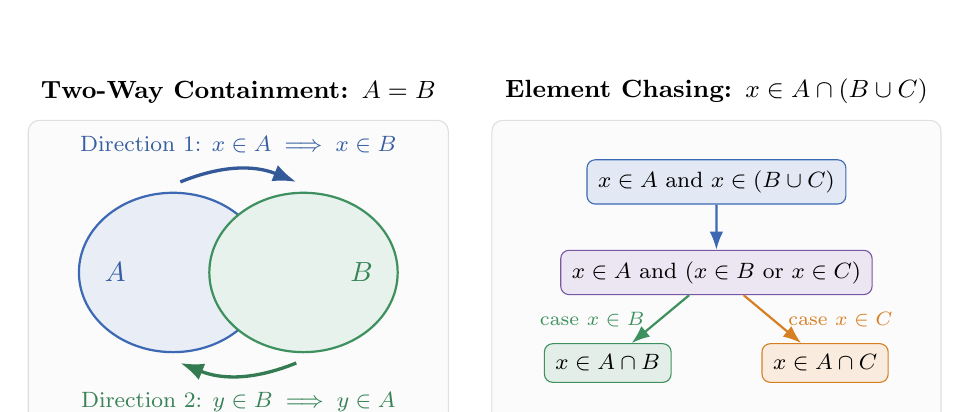
\begin{tikzpicture}[scale=0.92, >=Latex]
  % Panel 1: Double containment architecture
  \begin{scope}[xshift=0cm]
    \draw[rounded corners=4pt, fill=gray!3, draw=gray!25] (-0.4, -0.7) rectangle (5.4, 3.5);
    \node[anchor=south, font=\small\bfseries] at (2.5, 3.6) {Two-Way Containment: $A = B$};
    
    % Sets A and B
    \draw[thick, sourceblue, fill=sourceblue!12] (1.6, 1.4) ellipse (1.3cm and 1.1cm);
    \draw[thick, targetgreen, fill=targetgreen!12] (3.4, 1.4) ellipse (1.3cm and 1.1cm);
    
    \node[sourceblue!90!black, font=\bfseries] at (0.8, 1.4) {$A$};
    \node[targetgreen!90!black, font=\bfseries] at (4.2, 1.4) {$B$};
    
    % Direction arrows
    \draw[->, very thick, sourceblue!85!black] (1.7, 2.65) to[bend left=22] node[above=2pt, font=\footnotesize, text=sourceblue!90!black] {Direction 1: $x \in A \implies x \in B$} (3.3, 2.65);
    \draw[->, very thick, targetgreen!85!black] (3.3, 0.15) to[bend left=22] node[below=2pt, font=\footnotesize, text=targetgreen!90!black] {Direction 2: $y \in B \implies y \in A$} (1.7, 0.15);
  \end{scope}

  % Panel 2: Element chase through distribution
  \begin{scope}[xshift=6.4cm]
    \draw[rounded corners=4pt, fill=gray!3, draw=gray!25] (-0.4, -0.7) rectangle (5.8, 3.5);
    \node[anchor=south, font=\small\bfseries] at (2.7, 3.6) {Element Chasing: $x \in A \cap (B \cup C)$};

    % Tracking path
    \node[draw=sourceblue, fill=sourceblue!15, rounded corners=3pt, font=\footnotesize, inner sep=4pt] (start) at (2.7, 2.65) {$x \in A \text{ and } x \in (B \cup C)$};
    \node[draw=structurepurple, fill=structurepurple!15, rounded corners=3pt, font=\footnotesize, inner sep=4pt] (branch) at (2.7, 1.4) {$x \in A \text{ and } (x \in B \text{ or } x \in C)$};
    
    \node[draw=targetgreen, fill=targetgreen!15, rounded corners=3pt, font=\footnotesize, inner sep=4pt] (left) at (1.2, 0.15) {$x \in A \cap B$};
    \node[draw=quotientorange, fill=quotientorange!15, rounded corners=3pt, font=\footnotesize, inner sep=4pt] (right) at (4.2, 0.15) {$x \in A \cap C$};
    
    \draw[->, thick, sourceblue] (start) -- (branch);
    \draw[->, thick, targetgreen] (branch) -- node[left=2pt, font=\scriptsize] {case $x \in B$} (left);
    \draw[->, thick, quotientorange] (branch) -- node[right=2pt, font=\scriptsize] {case $x \in C$} (right);
  \end{scope}
\end{tikzpicture}
\caption{The two foundational architectures of set proofs. \textbf{Left}: Demonstrating set equality $A = B$ requires establishing mutual subset inclusion in two independent directions---first showing that every $x \in A$ must belong to $B$, and then showing that every $y \in B$ must belong to $A$. \textbf{Right}: Chasing an element through compound logical conditions. When the hypothesis contains a union ($B \cup C$), logic presents an ``or'' (disjunction $\lor$), causing the chase to branch into exhaustive cases that each reach the target set.}
\label{11:fig-double-containment}
\end{figure}

\begin{intuitionbox}
Think of element chasing as reasoning about an arbitrary element $x$. You do not pick a specific number like $x = 0$ or $x = 5$. You write ``Let $x \in A$,'' using only the properties guaranteed by membership in $A$. If you can deduce from those properties that $x \in B$, then every element of $A$ must belong to $B$.
\end{intuitionbox}

\subsection{A Warm-Up: Intersection Subsets}

Let us start with the most basic structural property of intersections.

\begin{theorem}
For any sets $A$ and $B$, $A \cap B \subseteq A$.
\end{theorem}

\begin{proof}
Let $x \in A \cap B$ be arbitrary. 

By definition of intersection, $x \in A \cap B$ means that $x \in A$ and $x \in B$. 

In formal logic, a statement joined by ``and'' is called a \emph{conjunction} ($P \land Q$). From the conjunction $x \in A \land x \in B$, the single statement $x \in A$ follows immediately by simplification (if both facts are true, each one is true on its own). 

Since $x$ was an arbitrary element of $A \cap B$, every element of $A \cap B$ belongs to $A$. Thus $A \cap B \subseteq A$.
\end{proof}

Notice how clean the flow is: we assumed $x \in A \cap B$, unwrapped the definition into a logical statement, extracted what was needed, and concluded containment.

\begin{intuitionbox}
\textbf{Pause and think:} Why couldn't we prove $A \cap B \subseteq A$ by testing concrete sets, say $A = \{1, 2, 3\}$ and $B = \{2, 3, 4\}$, calculating $A \cap B = \{2, 3\}$, and observing that both $2$ and $3$ belong to $A$? Because testing concrete numbers only checks that specific example. To establish a universal claim ($(\forall x)(x \in A \cap B \implies x \in A)$), the element $x$ must be generic, possessing only the properties guaranteed by membership in $A \cap B$.
\end{intuitionbox}

\subsection{Set Difference as Complementation}

Next, consider the relationship between set difference and the complement. Before we can talk about a complement, we must specify an ambient \emph{universal set} $U$---the overarching background universe of objects under discussion (such as the real numbers $\R$ or the integers $\Z$). 

The \emph{complement} of a set $B$, denoted $B^c$, consists of all objects in $U$ that lie strictly outside $B$:
\[
B^c = \{x \in U : x \notin B\}.
\]
The \emph{set difference} $A \setminus B$ (read ``$A$ minus $B$'') consists of all elements that belong to $A$ with anything belonging to $B$ discarded:
\[
A \setminus B = \{x \in U : x \in A \text{ and } x \notin B\}.
\]
How do these two concepts interact? Removing $B$ from $A$ turns out to be exactly the same as intersecting $A$ with everything outside $B$.

\begin{theorem}
Let $A$ and $B$ be subsets of a universal set $U$. Then
\[
A \setminus B = A \cap B^c.
\]
\end{theorem}

Figure~\ref{11:fig-difference-complementation} illustrates this identity: whether you start with $A$ and remove $B$, or take the intersection of $A$ with the exterior of $B$ ($B^c$), the resulting territory is identical.

\begin{figure}[htbp]
\centering
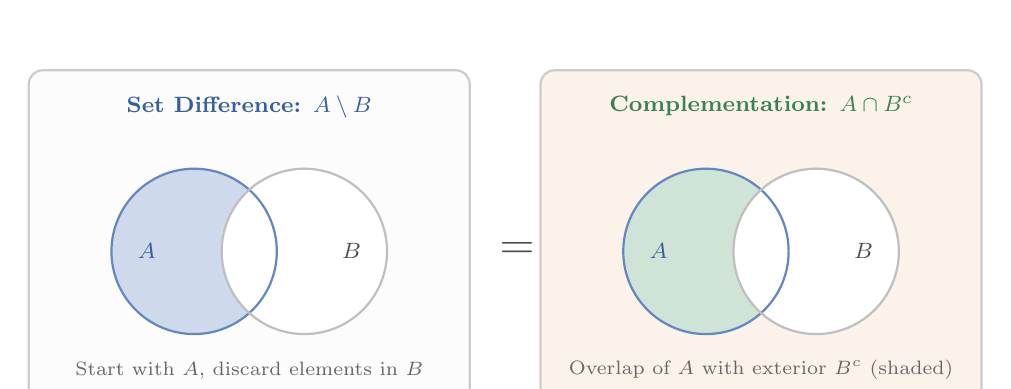
\begin{tikzpicture}[
    font=\small,
    univ/.style={draw=gray!40, fill=gray!2, rounded corners=5pt, thick}
]

% Panel 1: A \ B
\begin{scope}[xshift=0cm]
    \draw[univ] (-0.3, -0.6) rectangle (5.3, 3.6);

    % Fills first
    \fill[sourceblue!25] (1.8, 1.3) circle (1.05);
    \fill[white] (3.2, 1.3) circle (1.05);

    % Outlines
    \draw[thick, sourceblue!80] (1.8, 1.3) circle (1.05);
    \draw[thick, gray!50] (3.2, 1.3) circle (1.05);

    % Labels last
    \node[anchor=north, font=\footnotesize\bfseries, text=sourceblue!90!black] at (2.5, 3.4) {Set Difference: $A \setminus B$};
    \node[font=\footnotesize\bfseries, text=sourceblue!90!black] at (1.2, 1.3) {$A$};
    \node[font=\footnotesize\bfseries, text=gray!60!black] at (3.8, 1.3) {$B$};

    \node[anchor=south, font=\scriptsize, text=gray!80!black] at (2.5, -0.45) {Start with $A$, discard elements in $B$};
\end{scope}

% Equals symbol
\node[font=\LARGE\bfseries, text=gray!60!black] at (5.9, 1.3) {$=$};

% Panel 2: A \cap B^c
\begin{scope}[xshift=6.5cm]
    % Background box with B^c shading first
    \draw[draw=gray!40, fill=quotientorange!10, rounded corners=5pt, thick] (-0.3, -0.6) rectangle (5.3, 3.6);
    \fill[white] (3.2, 1.3) circle (1.05);

    % Intersection A \cap B^c fill
    \begin{scope}
        \clip (1.8, 1.3) circle (1.05);
        \fill[targetgreen!25] (1.8, 1.3) circle (1.05);
        \fill[white] (3.2, 1.3) circle (1.05);
    \end{scope}

    % Outlines
    \draw[thick, sourceblue!80] (1.8, 1.3) circle (1.05);
    \draw[thick, gray!50] (3.2, 1.3) circle (1.05);

    % Labels last
    \node[anchor=north, font=\footnotesize\bfseries, text=targetgreen!90!black] at (2.5, 3.4) {Complementation: $A \cap B^c$};
    \node[font=\footnotesize\bfseries, text=sourceblue!90!black] at (1.2, 1.3) {$A$};
    \node[font=\footnotesize\bfseries, text=gray!60!black] at (3.8, 1.3) {$B$};

    \node[anchor=south, font=\scriptsize, text=gray!80!black] at (2.5, -0.45) {Overlap of $A$ with exterior $B^c$ (shaded)};
\end{scope}

\end{tikzpicture}
\caption{Geometric equivalence of set difference and complementation ($A \setminus B = A \cap B^c$). On the left, we begin with $A$ and remove all points of $B$. On the right, we intersect $A$ with the exterior region $B^c$ (shaded in light orange). Both operations isolate the identical blue-green territory.}\label{11:fig-difference-complementation}
\end{figure}

\begin{proof}
We will prove this equality by demonstrating that an arbitrary element $x \in U$ belongs to the left-hand side if and only if it belongs to the right-hand side.

Let $x \in U$ be arbitrary. Then:
\begin{align*}
x \in A \setminus B 
&\iff x \in A \text{ and } x \notin B && \text{(definition of set difference)} \\
&\iff x \in A \text{ and } x \in B^c && \text{(definition of complement)} \\
&\iff x \in A \cap B^c && \text{(definition of intersection)}.
\end{align*}
Because each step is a bidirectional logical equivalence ($\iff$), the two sets contain exactly the same elements. Hence $A \setminus B = A \cap B^c$.
\end{proof}

\begin{trapbox}
Chaining if-and-only-if ($\iff$) statements is elegant when every step is truly reversible. But be careful: if even a single step only holds in one direction (for instance, $x \in S \implies x \in S \cup T$, which cannot be reversed), the whole two-way proof collapses. When in doubt, split the proof into two explicit halves: first assume $x$ is in the left set and deduce it is in the right, then assume $x$ is in the right set and deduce it is in the left.
\end{trapbox}

\subsection{Distributing Intersection Over Union}

In basic algebra, multiplication distributes across addition: $a \cdot (b + c) = (a \cdot b) + (a \cdot c)$. In set theory, intersection distributes across union in the same way:
\[
A \cap (B \cup C) = (A \cap B) \cup (A \cap C).
\]
Why does proving this identity require a case-by-case argument? When an element $x$ belongs to a union $B \cup C$, logic presents us with a \emph{disjunction} ($P \lor Q$)---the condition that $x \in B$ or $x \in C$. Unlike a conjunction (``and''), which allows us to hold both facts simultaneously, a disjunction offers two alternative possibilities. Since we do not know in advance which condition $x$ satisfies, we consider each case separately and verify that in both cases $x$ belongs to $(A \cap B) \cup (A \cap C)$.

\begin{theorem}
For all sets $A, B$, and $C$,
\[
A \cap (B \cup C) = (A \cap B) \cup (A \cap C).
\]
\end{theorem}

Figure~\ref{11:fig-distributive-branching} contrasts the spatial intuition with the formal logical architecture: because union introduces an ``or'' condition, the forward element chase must split into two parallel cases that independently reach the destination.

\begin{figure}[htbp]
\centering
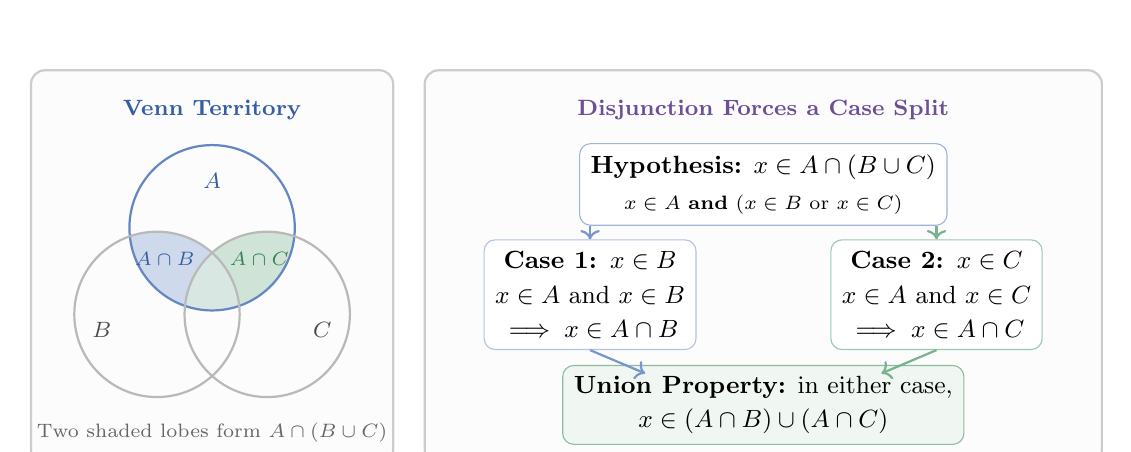
\begin{tikzpicture}[
    font=\small,
    univ/.style={draw=gray!40, fill=gray!2, rounded corners=5pt, thick},
    boxnode/.style={draw=gray!35, fill=white, rounded corners=4pt, inner sep=4pt, align=center}
]

% Panel 1: Geometric Venn Diagram
\begin{scope}[xshift=0cm]
    \draw[univ] (-0.3, -0.7) rectangle (4.3, 4.3);

    % Fills first
    \begin{scope}
        \clip (2.0, 2.3) circle (1.05);
        \fill[sourceblue!25] (1.3, 1.2) circle (1.05);
        \fill[targetgreen!25] (2.7, 1.2) circle (1.05);
        % Overlap region
        \begin{scope}
            \clip (1.3, 1.2) circle (1.05);
            \fill[sourceblue!20!targetgreen!20] (2.7, 1.2) circle (1.05);
        \end{scope}
    \end{scope}

    % Outlines
    \draw[thick, sourceblue!80] (2.0, 2.3) circle (1.05);
    \draw[thick, gray!55] (1.3, 1.2) circle (1.05);
    \draw[thick, gray!55] (2.7, 1.2) circle (1.05);

    % Labels last
    \node[anchor=north, font=\footnotesize\bfseries, text=sourceblue!90!black] at (2.0, 4.05) {Venn Territory};
    \node[font=\footnotesize\bfseries, text=sourceblue!90!black] at (2.0, 2.9) {$A$};
    \node[font=\footnotesize\bfseries, text=gray!60!black] at (0.6, 1.0) {$B$};
    \node[font=\footnotesize\bfseries, text=gray!60!black] at (3.4, 1.0) {$C$};

    \node[font=\scriptsize\bfseries, text=sourceblue!90!black] at (1.4, 1.9) {$A \cap B$};
    \node[font=\scriptsize\bfseries, text=targetgreen!90!black] at (2.6, 1.9) {$A \cap C$};

    \node[anchor=south, font=\scriptsize, text=gray!80!black] at (2.0, -0.55) {Two shaded lobes form $A \cap (B \cup C)$};
\end{scope}

% Panel 2: Logical Branching Diagram
\begin{scope}[xshift=4.9cm]
    \draw[univ] (-0.2, -0.7) rectangle (8.4, 4.3);

    \node[anchor=north, font=\footnotesize\bfseries, text=structurepurple!90!black] at (4.1, 4.05) {Disjunction Forces a Case Split};

    % Top node
    \node[boxnode, draw=sourceblue!50] (top) at (4.1, 2.85) {
        \textbf{Hypothesis:} $x \in A \cap (B \cup C)$ \\[2pt]
        {\scriptsize $x \in A$ \textbf{and} ($x \in B$ or $x \in C$)}
    };

    % Case 1 and Case 2 nodes
    \node[boxnode, draw=sourceblue!40] (c1) at (1.9, 1.45) {
        \textbf{Case 1: $x \in B$} \\[2pt]
        $x \in A$ and $x \in B$ \\[1pt]
        $\implies x \in A \cap B$
    };

    \node[boxnode, draw=targetgreen!50] (c2) at (6.3, 1.45) {
        \textbf{Case 2: $x \in C$} \\[2pt]
        $x \in A$ and $x \in C$ \\[1pt]
        $\implies x \in A \cap C$
    };

    % Conclusion node
    \node[boxnode, draw=targetgreen!60, fill=targetgreen!8] (bot) at (4.1, 0.05) {
        \textbf{Union Property:} in either case, \\[1pt]
        $x \in (A \cap B) \cup (A \cap C)$
    };

    % Arrows between nodes
    \draw[->, thick, sourceblue!70] (top.south -| c1.north) -- (c1.north);
    \draw[->, thick, targetgreen!70] (top.south -| c2.north) -- (c2.north);
    \draw[->, thick, sourceblue!70] (c1.south) -- (2.6, 0.45);
    \draw[->, thick, targetgreen!70] (c2.south) -- (5.6, 0.45);
\end{scope}

\end{tikzpicture}
\caption{Distributive law for sets ($A \cap (B \cup C) = (A \cap B) \cup (A \cap C)$). Left: the geometric overlap consists of two distinct regions, $A \cap B$ and $A \cap C$. Right: the element chase structure. Because membership in a union presents an ``or'' condition, the argument must branch into two exhaustive cases, each independently certifying membership in the target union.}\label{11:fig-distributive-branching}
\end{figure}

\begin{proof}
We prove mutual containment: first $A \cap (B \cup C) \subseteq (A \cap B) \cup (A \cap C)$, and then the reverse inclusion.

\textbf{Direction 1: $(\subseteq)$.} Let $x \in A \cap (B \cup C)$ be arbitrary. 
By definition of intersection, $x \in A$ and $x \in B \cup C$. 
Unpacking the union, $x \in B \cup C$ means $x \in B$ or $x \in C$. We now argue by cases:
\begin{itemize}
\item \emph{Case 1: $x \in B$.} Since we already know $x \in A$, we have $x \in A$ and $x \in B$, which means $x \in A \cap B$. It follows that $x \in (A \cap B) \cup (A \cap C)$.
\item \emph{Case 2: $x \in C$.} Since $x \in A$, we have $x \in A$ and $x \in C$, so $x \in A \cap C$. Therefore $x \in (A \cap B) \cup (A \cap C)$.
\end{itemize}
In either case, $x \in (A \cap B) \cup (A \cap C)$. This establishes that
\[
A \cap (B \cup C) \subseteq (A \cap B) \cup (A \cap C).
\]

\textbf{Direction 2: $(\supseteq)$.} Now let $y \in (A \cap B) \cup (A \cap C)$ be arbitrary.
By definition of union, $y \in A \cap B$ or $y \in A \cap C$. Again, we examine the two possibilities:
\begin{itemize}
\item \emph{Case 1: $y \in A \cap B$.} Then $y \in A$ and $y \in B$. Since $y \in B$, we certainly have $y \in B \cup C$. Combining $y \in A$ with $y \in B \cup C$ gives $y \in A \cap (B \cup C)$.
\item \emph{Case 2: $y \in A \cap C$.} Then $y \in A$ and $y \in C$. Since $y \in C$, we have $y \in B \cup C$. Hence $y \in A \cap (B \cup C)$.
\end{itemize}
In both cases, $y \in A \cap (B \cup C)$. Thus
\[
(A \cap B) \cup (A \cap C) \subseteq A \cap (B \cup C).
\]

Having established containment in both directions, we conclude that $A \cap (B \cup C) = (A \cap B) \cup (A \cap C)$.
\end{proof}

\begin{historybox}
In the 1760s, Leonhard Euler introduced closed circular curves to illustrate categorical syllogisms in logic. A century later, in an 1880 paper titled ``On the Diagrammatic and Mechanical Representation of Propositions and Reasonings,'' the English logician John Venn refined Euler's idea by requiring that all possible combinations of inclusion and exclusion among the sets be visually represented, even building mechanical wooden devices with sliding gears to model logical deductions. For two or three sets, Venn's diagrams are wonderfully clear. 

Yet mathematics quickly ran into hard geometric and conceptual barriers. First, Venn showed that while three sets can be drawn with congruent circles, four mutually intersecting sets cannot: congruent circles can only form $14$ of the required $16$ regions, forcing one to use distorted ellipses or interlocking ribbons. For five or more sets, constructing symmetric Venn diagrams made of congruent curves is mathematically impossible unless the number of sets $n$ is prime (proven by Anthony Edwards and Branko Gr\"unbaum).

Second, visual diagrams break down completely when confronted with infinite collections of sets, such as the shrinking sequence of intervals $\bigcap_{n=1}^\infty (-1/n, 1/n) = \{0\}$ in real analysis, where there are infinitely many boundaries. 

Element chasing replaced spatial inspection with formal symbolic deduction: reasoning about an arbitrary element $x$ applies equally well to two sets, twenty sets, or an arbitrary family of sets.
\end{historybox}

\subsection{Power Sets and Inclusion: Chasing Across Layers}

Element chasing also works when the elements themselves are sets. The \emph{power set} of a set $A$, denoted $\pow(A)$, is the collection whose elements are all possible subsets of $A$:
\[
X \in \pow(A) \iff X \subseteq A.
\]
For example, if $A = \{1, 2\}$, its subsets are $\emptyset, \{1\}, \{2\}$, and $\{1, 2\}$, so $\pow(A) = \{\emptyset, \{1\}, \{2\}, \{1, 2\}\}$. 

When we prove an inclusion between power sets, the element being chased is itself a set.

\begin{theorem}
If $A \subseteq B$, then $\pow(A) \subseteq \pow(B)$.
\end{theorem}

\begin{proof}
Suppose $A \subseteq B$. We want to show $\pow(A) \subseteq \pow(B)$.

Let $X \in \pow(A)$ be arbitrary. By definition of the power set, this means $X \subseteq A$.

Now we need to show that $X \in \pow(B)$, which means showing $X \subseteq B$. 

To show $X \subseteq B$, let $z \in X$ be an arbitrary element. Since $X \subseteq A$, we have $z \in A$. Since $A \subseteq B$, we have $z \in B$. Since every $z \in X$ belongs to $B$, we have $X \subseteq B$.

Therefore $X \in \pow(B)$. Because $X \in \pow(A)$ was arbitrary, $\pow(A) \subseteq \pow(B)$.
\end{proof}

\begin{figure}[htbp]
\centering
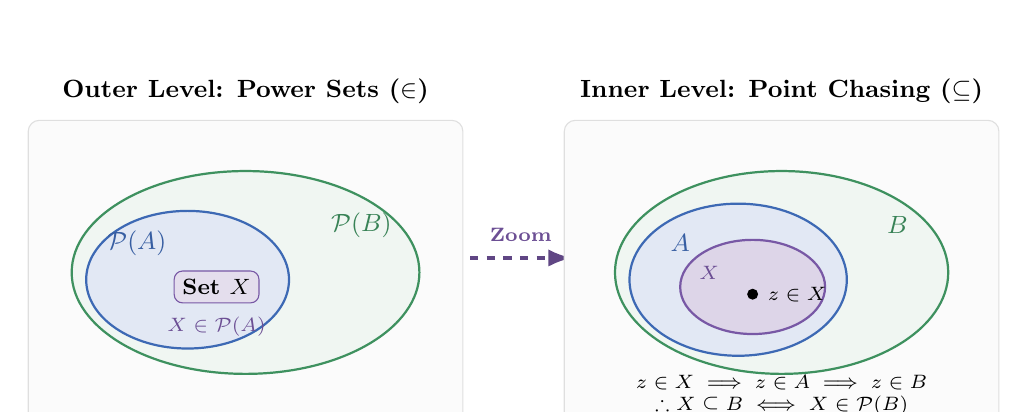
\begin{tikzpicture}[scale=0.92, >=Latex]
  % Panel 1: Outer Level (Power Sets)
  \begin{scope}[xshift=0cm]
    \draw[rounded corners=4pt, fill=gray!3, draw=gray!25] (-0.4, -0.7) rectangle (5.6, 3.5);
    \node[anchor=south, font=\small\bfseries] at (2.6, 3.6) {Outer Level: Power Sets ($\in$)};

    % Big ellipse: P(B)
    \draw[thick, targetgreen, fill=targetgreen!8] (2.6, 1.4) ellipse (2.4cm and 1.4cm);
    \node[targetgreen!90!black, font=\bfseries\small] at (4.2, 2.05) {$\pow(B)$};

    % Smaller ellipse: P(A)
    \draw[thick, sourceblue, fill=sourceblue!15] (1.8, 1.3) ellipse (1.4cm and 0.95cm);
    \node[sourceblue!90!black, font=\bfseries\small] at (1.1, 1.8) {$\pow(A)$};

    % The element X inside P(A)
    \node[draw=structurepurple, fill=structurepurple!20, rounded corners=3pt, inner sep=3pt, font=\footnotesize\bfseries] (Xnode) at (2.2, 1.2) {Set $X$};
    \node[font=\scriptsize, structurepurple!90!black] at (2.2, 0.65) {$X \in \pow(A)$};
  \end{scope}

  % Zoom connector between panels
  \draw[->, very thick, dashed, structurepurple!80!black] (5.7, 1.6) -- node[above=2pt, font=\scriptsize\bfseries, text=structurepurple!90!black] {Zoom} (7.1, 1.6);

  % Panel 2: Inner Level (Points inside Sets)
  \begin{scope}[xshift=7.4cm]
    \draw[rounded corners=4pt, fill=gray!3, draw=gray!25] (-0.4, -0.7) rectangle (5.6, 3.5);
    \node[anchor=south, font=\small\bfseries] at (2.6, 3.6) {Inner Level: Point Chasing ($\subseteq$)};

    % Set B
    \draw[thick, targetgreen, fill=targetgreen!8] (2.6, 1.4) ellipse (2.3cm and 1.4cm);
    \node[targetgreen!90!black, font=\bfseries\small] at (4.2, 2.05) {$B$};

    % Set A
    \draw[thick, sourceblue, fill=sourceblue!15] (2.0, 1.3) ellipse (1.5cm and 1.05cm);
    \node[sourceblue!90!black, font=\bfseries\small] at (1.2, 1.8) {$A$};

    % Set X inside A
    \draw[thick, structurepurple, fill=structurepurple!25] (2.2, 1.2) ellipse (1.0cm and 0.65cm);
    \node[structurepurple!90!black, font=\scriptsize\bfseries] at (1.6, 1.4) {$X$};

    % Point z inside X
    \node[circle, fill=black, inner sep=1.4pt] (zpt) at (2.2, 1.1) {};
    \node[right=2pt, font=\scriptsize, text=black] at (2.2, 1.1) {$z \in X$};
    
    \node[font=\scriptsize, align=center] at (2.6, -0.3) {$z \in X \implies z \in A \implies z \in B$\\$\therefore X \subseteq B \iff X \in \pow(B)$};
  \end{scope}
\end{tikzpicture}
\caption{Two levels of element chasing in power sets. \textbf{Left}: At the outer level, the element is a set $X$ satisfying $X \in \pow(A)$. \textbf{Right}: To show $X \subseteq B$, we consider an arbitrary element $z \in X$. Since $X \subseteq A$ and $A \subseteq B$, we deduce $z \in B$, establishing $X \subseteq B$ and therefore $X \in \pow(B)$.}
\label{11:fig-power-set-levels}
\end{figure}

\begin{labbox}
Notice the two layers of element chasing in the proof above (illustrated in Figure~\ref{11:fig-power-set-levels})! At the outer level, the element is a set $X$ moving from $\pow(A)$ to $\pow(B)$. At the inner level, the element is a point $z$ moving from $X$ to $B$. Keeping these levels distinct prevents the common beginner mistake of confusing $\in$ with $\subseteq$.
\end{labbox}

\begin{intuitionbox}
\textbf{Pause and think:} What happens in the extreme case where $A = \emptyset$? Does Theorem~4 still hold? Yes! The empty set has only one subset: itself ($\pow(\emptyset) = \{\emptyset\}$). If $A = \emptyset$, then $A \subseteq B$ is vacuously true for every set $B$, and since $\emptyset \subseteq B$, we have $\emptyset \in \pow(B)$. Thus $\{\emptyset\} \subseteq \pow(B)$, confirming that $\pow(\emptyset) \subseteq \pow(B)$ as required.
\end{intuitionbox}

\subsection{Scope of element chasing and the transition to functions}

Element chasing provides a direct method to verify set identities, Boolean laws, and subset inclusions. It replaces visual diagrams with rigorous logical deduction.

Sets and element chasing describe static collections and containment, but most of mathematics concerns how elements of one set are sent to elements of another---and whether those transformations preserve algebraic, geometric, or topological structure. In Chapter~12 (\emph{Functions: Structured Promises, Not Just Formulas}), we study functions, the precise rules that map inputs in one set to outputs in another.

\subsection{Exercises}

\subsubsection*{Warm-Up Mental Checks}
\begin{enumerate}[label=\arabic*.]
\item \textbf{The One-Way Trap:} A student writes: ``$x \in A \cup B \iff x \in A$, therefore $A \cup B \subseteq A$.'' Where is the exact logical flaw? Can you give a simple counterexample with numbers where $x \in A \cup B$ is true but $x \in A$ is false?
\item \textbf{Power Set Distinctions:} Let $A = \{1, 2\}$. For each of the following statements, decide whether it is true or false, and explain the difference between them in your own words:
\begin{enumerate}[label=(\alph*)]
\item $\emptyset \in \pow(A)$
\item $\emptyset \subseteq \pow(A)$
\item $\{\emptyset\} \subseteq \pow(A)$
\end{enumerate}
\item \textbf{Proving Emptiness:} Suppose you want to prove that a set $S$ is empty ($S = \emptyset$). How can you adapt the element-chasing method to achieve this? (Hint: Assume for contradiction that there exists some $x \in S$, and chase this hypothetical element until you deduce a logical impossibility.)
\end{enumerate}

\subsubsection*{Core Practice: Element-Chasing Proofs}
Write out complete proofs using full grammatical sentences, explicitly introducing every arbitrary element.
\begin{enumerate}[resume*]
\item Prove that for any sets $A$ and $B$, $A \subseteq A \cup B$.
\item Prove that $A \cap (B \setminus C) = (A \cap B) \setminus C$.
\item Prove De Morgan's Law for set difference across unions:
\[
A \setminus (B \cup C) = (A \setminus B) \cap (A \setminus C).
\]
\item Prove the companion De Morgan identity for set difference across intersections:
\[
A \setminus (B \cap C) = (A \setminus B) \cup (A \setminus C).
\]
\end{enumerate}

\subsubsection*{Deeper Explorations}
\begin{enumerate}[resume*]
\item \textbf{Power Sets and Intersections:} Prove that for all sets $A$ and $B$,
\[
\pow(A \cap B) = \pow(A) \cap \pow(B).
\]
\item \textbf{Power Sets and Unions:} What happens if we replace intersection with union in the previous problem?
\begin{enumerate}[label=(\alph*)]
\item Prove that $\pow(A) \cup \pow(B) \subseteq \pow(A \cup B)$ always holds.
\item Give an explicit counterexample with small finite sets to prove that the reverse containment, $\pow(A \cup B) \subseteq \pow(A) \cup \pow(B)$, is generally false.
\end{enumerate}
\item \textbf{Infinite Families:} Let $\{A_i\}_{i \in I}$ be an indexed family of sets (where the index set $I$ may be finite or infinite), and let $B$ be a set. Recall that an element belongs to an arbitrary intersection $\bigcap_{i \in I} S_i$ if and only if it belongs to $S_i$ for every $i \in I$. Prove that:
\[
\left( \bigcap_{i \in I} A_i \right) \cap B = \bigcap_{i \in I} (A_i \cap B).
\]
Notice how tracking an arbitrary element $x$ works for an arbitrary indexed family just as it does for two sets.
\end{enumerate}

\newpage

\section{Functions: Structured Promises, Not Just Formulas}
\chapterline

In elementary algebra and calculus, a function is almost always introduced as an algebraic formula: an expression like $f(x) = x^2$ or $g(x) = \sin(x) / x$. You plug a real number into the machine, turn the symbolic crank, and read off the computed result.

In pure mathematics, that formula-centric perspective is entirely too narrow. A formula is merely an algorithm or assignment rule. A \emph{function} is a structured contract between two mathematical sets. It is a promise that transforms an entire universe of inputs into a declared destination space, obeying strict geometric and logical rules.

\begin{historybox}
The modern definition of a function was forged through a century of fierce mathematical debate. In 1718, Johann Bernoulli defined a function as ``any quantity composed in whatever manner of a variable and constants.'' Thirty years later, Leonhard Euler (\emph{Introductio in analysin infinitorum}, 1748) codified functions as expressions formed by algebraic operations or infinite series. 

This formula-based view triggered the famous 18th-century ``vibrating string controversy'' between Jean le Rond d'Alembert, Euler, and Daniel Bernoulli. If a plucked violin string is released from an initial triangular shape with a sharp corner, can that physical motion be described by a function? Euler argued that a curve with a corner could not be a genuine function because it had no single continuous differential equation. 

The breakthrough came in 1829 from Peter Gustav Lejeune Dirichlet while studying the convergence of Fourier series. Dirichlet realized that mathematics had to sever the concept of a function from the demand for an algebraic formula. A function, Dirichlet proposed, is simply an arbitrary assignment that pairs every input $x$ with a unique output $y$. To prove how far this extended beyond formulas, he introduced the notorious Dirichlet function:
\[
\mathbf{1}_\mathbb{Q}(x) = \begin{cases} 1 & \text{if } x \in \mathbb{Q}, \\ 0 & \text{if } x \notin \mathbb{Q}. \end{cases}
\]
Dirichlet's function has no algebraic formula, cannot be drawn with a pen, and is discontinuous at every single real number! Traditionalists were horrified; Charles Hermite famously lamented, ``I turn away with fright and horror from this lamentable plague of functions which have no derivatives.'' Yet Dirichlet was right. Richard Dedekind and later Nicolas Bourbaki (1939) cemented this insight in modern set theory: a function is not an algebraic equation, but a lawful subset of a Cartesian product.
\end{historybox}

\subsection{The Anatomy of a Function}

Formally, a function consists of three distinct components:
\begin{enumerate}[label=\arabic*.]
\item A set $A$ called the \textbf{domain} (the universe of allowed inputs).
\item A set $B$ called the \textbf{codomain} (the designated target space).
\item A relation or rule that assigns to \textbf{every} element $a \in A$ \textbf{exactly one} element $b \in B$, denoted $f(a) = b$.
\end{enumerate}

We package this entire tripartite package in the standard notation:
\[
f: A \to B.
\]

\begin{definition}[Function]
A function $f: A \to B$ is a relation from $A$ to $B$ satisfying two structural conditions:
\begin{enumerate}[label=(\roman*)]
\item \textbf{Total Definition:} For every $a \in A$, there exists some $b \in B$ such that $f(a) = b$.
\item \textbf{Single-Valuedness:} For every $a \in A$ and all $b_1, b_2 \in B$, if $f(a) = b_1$ and $f(a) = b_2$, then $b_1 = b_2$.
\end{enumerate}
\end{definition}

\begin{center}
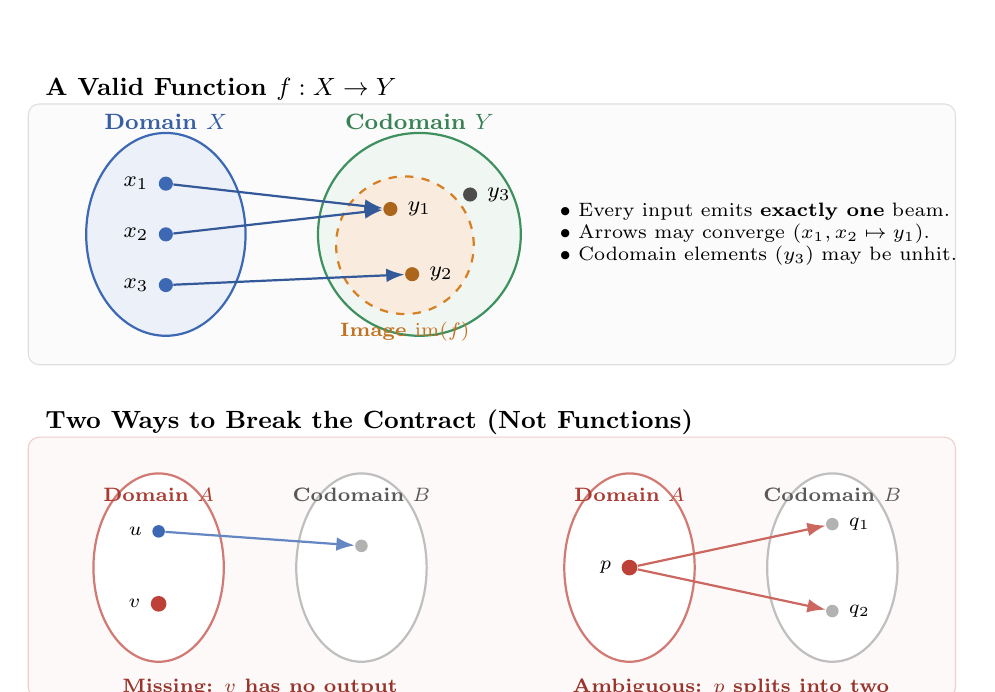
\begin{tikzpicture}[scale=0.92, >=Latex]
  % Lane 1: A Valid Function
  \begin{scope}[yshift=0cm]
    \node[anchor=west, font=\small\bfseries] at (-0.5, 3.2) {A Valid Function $f: X \to Y$};
    \draw[rounded corners=4pt, fill=gray!3, draw=gray!25] (-0.6, -0.6) rectangle (12.2, 3.0);
    
    % Domain X
    \draw[thick, sourceblue, fill=sourceblue!10] (1.3, 1.2) ellipse (1.1cm and 1.4cm);
    \node[sourceblue!90!black, font=\footnotesize\bfseries] at (1.3, 2.75) {Domain $X$};
    
    % Codomain Y
    \draw[thick, targetgreen, fill=targetgreen!8] (4.8, 1.2) ellipse (1.4cm and 1.4cm);
    \node[targetgreen!90!black, font=\footnotesize\bfseries] at (4.8, 2.75) {Codomain $Y$};
    
    % Image subset
    \draw[thick, dashed, quotientorange, fill=quotientorange!15] (4.6, 1.05) ellipse (0.95cm and 0.95cm);
    \node[quotientorange!90!black, font=\scriptsize\bfseries] at (4.6, -0.15) {Image $\operatorname{im}(f)$};
    
    % Points in X
    \node[circle, fill=sourceblue, inner sep=1.8pt, label={left:\footnotesize $x_1$}] (x1) at (1.3, 1.9) {};
    \node[circle, fill=sourceblue, inner sep=1.8pt, label={left:\footnotesize $x_2$}] (x2) at (1.3, 1.2) {};
    \node[circle, fill=sourceblue, inner sep=1.8pt, label={left:\footnotesize $x_3$}] (x3) at (1.3, 0.5) {};
    
    % Points in Y
    \node[circle, fill=quotientorange!80!black, inner sep=1.8pt, label={right:\footnotesize $y_1$}] (y1) at (4.4, 1.55) {};
    \node[circle, fill=quotientorange!80!black, inner sep=1.8pt, label={right:\footnotesize $y_2$}] (y2) at (4.7, 0.65) {};
    \node[circle, fill=gray!60!black, inner sep=1.8pt, label={right:\footnotesize $y_3$}] (y3) at (5.5, 1.75) {};
    
    % Arrows
    \draw[->, thick, sourceblue!85!black] (x1) -- (y1);
    \draw[->, thick, sourceblue!85!black] (x2) -- (y1);
    \draw[->, thick, sourceblue!85!black] (x3) -- (y2);
    
    \node[anchor=west, font=\scriptsize, align=left] at (6.6, 1.2) {
      $\bullet$ Every input emits \textbf{exactly one} beam.\\
      $\bullet$ Arrows may converge ($x_1, x_2 \mapsto y_1$).\\
      $\bullet$ Codomain elements ($y_3$) may be unhit.
    };
  \end{scope}

  % Lane 2: Broken Contracts (Non-Functions)
  \begin{scope}[yshift=-4.6cm]
    \node[anchor=west, font=\small\bfseries] at (-0.5, 3.2) {Two Ways to Break the Contract (Not Functions)};
    \draw[rounded corners=4pt, fill=trapred!3, draw=trapred!25] (-0.6, -0.6) rectangle (12.2, 3.0);
    
    % Panel A: Missing an output
    \begin{scope}[xshift=0cm]
      \draw[thick, trapred!70, fill=white] (1.2, 1.2) ellipse (0.9cm and 1.3cm);
      \node[trapred!90!black, font=\scriptsize\bfseries] at (1.2, 2.2) {Domain $A$};
      \draw[thick, gray!50, fill=white] (4.0, 1.2) ellipse (0.9cm and 1.3cm);
      \node[gray!70!black, font=\scriptsize\bfseries] at (4.0, 2.2) {Codomain $B$};
      
      \node[circle, fill=sourceblue, inner sep=1.6pt, label={left:\scriptsize $u$}] (u) at (1.2, 1.7) {};
      \node[circle, fill=trapred, inner sep=2pt, label={left:\scriptsize\bfseries $v$}] (v) at (1.2, 0.7) {};
      \node[circle, fill=gray!60, inner sep=1.6pt] (w) at (4.0, 1.5) {};
      
      \draw[->, thick, sourceblue!80] (u) -- (w);
      \node[below, trapred!80!black, font=\scriptsize\bfseries] at (2.6, -0.2) {Missing: $v$ has no output};
    \end{scope}
    
    % Panel B: Ambiguous multiple outputs
    \begin{scope}[xshift=6.5cm]
      \draw[thick, trapred!70, fill=white] (1.2, 1.2) ellipse (0.9cm and 1.3cm);
      \node[trapred!90!black, font=\scriptsize\bfseries] at (1.2, 2.2) {Domain $A$};
      \draw[thick, gray!50, fill=white] (4.0, 1.2) ellipse (0.9cm and 1.3cm);
      \node[gray!70!black, font=\scriptsize\bfseries] at (4.0, 2.2) {Codomain $B$};
      
      \node[circle, fill=trapred, inner sep=2pt, label={left:\scriptsize\bfseries $p$}] (p) at (1.2, 1.2) {};
      \node[circle, fill=gray!60, inner sep=1.6pt, label={right:\scriptsize $q_1$}] (q1) at (4.0, 1.8) {};
      \node[circle, fill=gray!60, inner sep=1.6pt, label={right:\scriptsize $q_2$}] (q2) at (4.0, 0.6) {};
      
      \draw[->, thick, trapred!80] (p) -- (q1);
      \draw[->, thick, trapred!80] (p) -- (q2);
      \node[below, trapred!80!black, font=\scriptsize\bfseries] at (2.6, -0.2) {Ambiguous: $p$ splits into two};
    \end{scope}
  \end{scope}
\end{tikzpicture}
\end{center}

\begin{intuitionbox}
Think of the domain as an array of laser pointers, and the codomain as a screen across the room. A valid function requires every single laser pointer to be switched on, and each pointer must project a clean, single dot on the screen. It is completely acceptable for two different lasers to shine on the same spot, or for parts of the screen to remain unlit. But a laser cannot be left dark, and a laser cannot shoot a beam that splits into two separate targets.
\end{intuitionbox}

\subsection{Why the Formula Alone Is Incomplete}

Consider the squaring formula $x \mapsto x^2$. Stating only the formula leaves out the actual behavior of the function. Watch how drastically the object transforms as we alter the domain and codomain:

\begin{itemize}
\item \textbf{Function 1:} $f: \R \to \R$ with $f(x) = x^2$. 
Because negative numbers produce positive squares, $f(-2) = f(2) = 4$. Multiple inputs collide on the same output. Furthermore, negative numbers in the codomain like $-7$ never get hit.
\item \textbf{Function 2:} $g: \R \to [0, \infty)$ with $g(x) = x^2$.
Here, the codomain has been trimmed to match the actual outputs. Every target $y \ge 0$ is reached by at least one input ($x = \sqrt{y}$), but collisions still occur ($g(-2) = g(2)$).
\item \textbf{Function 3:} $h: [0, \infty) \to [0, \infty)$ with $h(x) = x^2$.
Now negative inputs are eliminated from the domain. Collisions are gone, and every target in the codomain is hit. This function has an exact two-way inverse: $h^{-1}(y) = \sqrt{y}$.
\end{itemize}

Even though all three functions share the identical formula $x^2$, $f$ is neither invertible nor surjective, $g$ is surjective but not injective, and $h$ is a perfect bijection. Domain and codomain are not incidental metadata; they define what the function is.

\subsection{Codomain Versus Image}

One of the most persistent hurdles for beginners is confusing the \emph{codomain} with the \emph{image} (often called the range).

\begin{definition}[Image]
Let $f: A \to B$ be a function. The \textbf{image} of $f$, denoted $\operatorname{im}(f)$ or $f(A)$, is the subset of the codomain consisting of values that are actually achieved:
\[
\operatorname{im}(f) = \{f(a) \in B : a \in A\} = \{b \in B : (\exists a \in A)(f(a) = b)\}.
\]
\end{definition}

The codomain $B$ is the room you chose to throw darts in; the image $\operatorname{im}(f)$ is the collection of dart holes on the wall. The image is always a subset of the codomain:
\[
\operatorname{im}(f) \subseteq B.
\]
When every point in the codomain receives a dart ($\operatorname{im}(f) = B$), the function is called \emph{surjective}.

\subsection{Connection to Software Engineering}

In computer science, a function's domain and codomain correspond directly to its type signature:
\begin{center}
\texttt{function processData(x: InputType): ReturnType}
\end{center}
Declaring \texttt{ReturnType} as \texttt{int64} does not mean the function produces every possible 64-bit integer; it guarantees that whatever it returns will live within that set. A bug where a function throws an unhandled exception for some input is a failure of total definition. A function that behaves non-deterministically without explicit random state violates single-valuedness.

\subsection{What Modern Functions Unlocked, Their Limits, and Where We Go Next}

Freeing functions from formulas unlocked vast domains of modern science. It gave mathematicians the power to define discrete state-machine transitions, characteristic indicator functions in probability, piecewise step voltages in signal processing, and cryptographic permutations—none of which can be written as smooth algebraic expressions. It transformed mathematics from a catalog of formulas into a science of lawful transformations.

Yet knowing that an assignment $f: A \to B$ is a valid function tells you surprisingly little about the quality of the transformation:
\begin{itemize}
\item \textbf{Information loss:} A function is entirely permitted to map every single element of a million-element domain to the number $0$. It satisfies the definition of a function perfectly, but it completely obliterates the structure of the input space.
\item \textbf{Coverage gaps:} The codomain could be the entire real line $\R$, while the actual outputs form only a tiny handful of numbers.
\item \textbf{Irreversibility:} If multiple inputs collide on the same output, you can never trace a result backward to find the original cause.
\end{itemize}

A valid function is only a raw, minimal promise. To know whether a mapping preserves information, covers its destination, or can be undone, we need sharper structural tools. In Chapter~13, we introduce \textbf{Injective, Surjective, Bijective}, establishing the three fundamental pillars that govern collision-free mappings, target coverage, and invertible pairs.

\subsection{Exercises}

\begin{enumerate}
\item Determine whether each proposed rule defines a valid function. If not, state which property fails:
\begin{enumerate}[label=(\alph*)]
\item $f: \R \to \R$ defined by $f(x) = \frac{1}{x^2 - 4}$.
\item $g: \Q \to \Z$ defined by $g(p/q) = p + q$.
\item $h: \R \to \R$ defined by $h(x) = y$ where $y^2 = x$.
\end{enumerate}
\item Find the image of the function $f: \R \setminus \{1\} \to \R$ given by $f(x) = \frac{2x+1}{x-1}$. Is the number $2$ in the image?
\item Let $A = \{1, 2, 3\}$ and $B = \{a, b\}$. How many distinct functions exist from $A$ to $B$? How many distinct functions exist from $B$ to $A$?
\end{enumerate}

\newpage

\section{Injective, Surjective, Bijective}
\chapterline

Once you view a function as a mapping between two sets, three natural questions arise about its structural geometry:
\begin{enumerate}[label=\arabic*.]
\item \textbf{Do distinct inputs always land on distinct outputs?} Or do some paths merge and destroy information along the way?
\item \textbf{Does the mapping reach every corner of the codomain?} Or are some target elements permanently out of reach?
\item \textbf{Can the process be cleanly run in reverse?} Can we trace each output uniquely backward to the input that produced it?
\end{enumerate}

These three questions correspond to the three classical pillars of mapping theory: \emph{injectivity}, \emph{surjectivity}, and \emph{bijectivity}.

\begin{historybox}
Before the late nineteenth century, mathematicians had no universal vocabulary for classifying mappings. Equations were solved by algebraic manipulation, and invertibility was handled on an ad-hoc basis. The language of injective, surjective, and bijective maps emerged when Richard Dedekind and Georg Cantor confronted the profound mystery of the infinite.

In his groundbreaking 1888 treatise, \emph{Was sind und was sollen die Zahlen?} (``What are numbers and what should they be?''), Dedekind sought to define the natural numbers and infinity without relying on physical time, geometric space, or counting. His radical breakthrough was to define infinite sets purely through mapping properties: \emph{a set $S$ is infinite if and only if there exists an injective function $f: S \to S$ that is not surjective.} An infinite set is an object that can be squeezed into a proper subset of itself without any collisions! 

Simultaneously, Cantor employed bijections to accomplish what had previously seemed impossible: measuring the size (cardinality) of infinite collections without counting them one by one. By demonstrating that two sets share the same size if and only if there exists a bijective pairing between them, Cantor transformed functions from computational tools into the fundamental scales used to weigh infinity.
\end{historybox}

\begin{center}
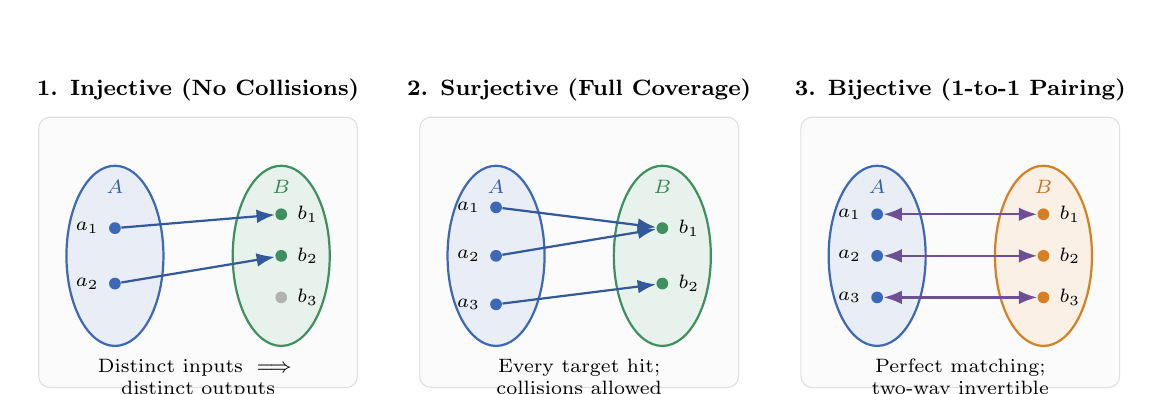
\begin{tikzpicture}[scale=0.88, >=Latex]
  % Panel 1: Injective
  \begin{scope}[xshift=0cm]
    \node[anchor=south, font=\footnotesize\bfseries] at (2.0, 3.4) {1. Injective (No Collisions)};
    \draw[rounded corners=4pt, fill=gray!3, draw=gray!25] (-0.3, -0.6) rectangle (4.3, 3.3);
    
    % Sets
    \draw[thick, sourceblue, fill=sourceblue!12] (0.8, 1.3) ellipse (0.7cm and 1.3cm);
    \draw[thick, targetgreen, fill=targetgreen!12] (3.2, 1.3) ellipse (0.7cm and 1.3cm);
    
    \node[sourceblue!90!black, font=\scriptsize\bfseries] at (0.8, 2.3) {$A$};
    \node[targetgreen!90!black, font=\scriptsize\bfseries] at (3.2, 2.3) {$B$};
    
    % Elements A
    \node[circle, fill=sourceblue, inner sep=1.5pt, label={left:\scriptsize $a_1$}] (i1) at (0.8, 1.7) {};
    \node[circle, fill=sourceblue, inner sep=1.5pt, label={left:\scriptsize $a_2$}] (i2) at (0.8, 0.9) {};
    
    % Elements B
    \node[circle, fill=targetgreen, inner sep=1.5pt, label={right:\scriptsize $b_1$}] (ib1) at (3.2, 1.9) {};
    \node[circle, fill=targetgreen, inner sep=1.5pt, label={right:\scriptsize $b_2$}] (ib2) at (3.2, 1.3) {};
    \node[circle, fill=gray!60, inner sep=1.5pt, label={right:\scriptsize $b_3$}] (ib3) at (3.2, 0.7) {};
    
    % Arrows
    \draw[->, thick, sourceblue!85!black] (i1) -- (ib1);
    \draw[->, thick, sourceblue!85!black] (i2) -- (ib2);
    
    \node[below, font=\scriptsize, align=center] at (2.0, -0.05) {Distinct inputs $\implies$\\distinct outputs};
  \end{scope}

  % Panel 2: Surjective
  \begin{scope}[xshift=5.5cm]
    \node[anchor=south, font=\footnotesize\bfseries] at (2.0, 3.4) {2. Surjective (Full Coverage)};
    \draw[rounded corners=4pt, fill=gray!3, draw=gray!25] (-0.3, -0.6) rectangle (4.3, 3.3);
    
    % Sets
    \draw[thick, sourceblue, fill=sourceblue!12] (0.8, 1.3) ellipse (0.7cm and 1.3cm);
    \draw[thick, targetgreen, fill=targetgreen!12] (3.2, 1.3) ellipse (0.7cm and 1.3cm);
    
    \node[sourceblue!90!black, font=\scriptsize\bfseries] at (0.8, 2.3) {$A$};
    \node[targetgreen!90!black, font=\scriptsize\bfseries] at (3.2, 2.3) {$B$};
    
    % Elements A
    \node[circle, fill=sourceblue, inner sep=1.5pt, label={left:\scriptsize $a_1$}] (s1) at (0.8, 2.0) {};
    \node[circle, fill=sourceblue, inner sep=1.5pt, label={left:\scriptsize $a_2$}] (s2) at (0.8, 1.3) {};
    \node[circle, fill=sourceblue, inner sep=1.5pt, label={left:\scriptsize $a_3$}] (s3) at (0.8, 0.6) {};
    
    % Elements B
    \node[circle, fill=targetgreen, inner sep=1.5pt, label={right:\scriptsize $b_1$}] (sb1) at (3.2, 1.7) {};
    \node[circle, fill=targetgreen, inner sep=1.5pt, label={right:\scriptsize $b_2$}] (sb2) at (3.2, 0.9) {};
    
    % Arrows
    \draw[->, thick, sourceblue!85!black] (s1) -- (sb1);
    \draw[->, thick, sourceblue!85!black] (s2) -- (sb1);
    \draw[->, thick, sourceblue!85!black] (s3) -- (sb2);
    
    \node[below, font=\scriptsize, align=center] at (2.0, -0.05) {Every target hit;\\collisions allowed};
  \end{scope}

  % Panel 3: Bijective
  \begin{scope}[xshift=11.0cm]
    \node[anchor=south, font=\footnotesize\bfseries] at (2.0, 3.4) {3. Bijective (1-to-1 Pairing)};
    \draw[rounded corners=4pt, fill=gray!3, draw=gray!25] (-0.3, -0.6) rectangle (4.3, 3.3);
    
    % Sets
    \draw[thick, sourceblue, fill=sourceblue!12] (0.8, 1.3) ellipse (0.7cm and 1.3cm);
    \draw[thick, quotientorange, fill=quotientorange!12] (3.2, 1.3) ellipse (0.7cm and 1.3cm);
    
    \node[sourceblue!90!black, font=\scriptsize\bfseries] at (0.8, 2.3) {$A$};
    \node[quotientorange!90!black, font=\scriptsize\bfseries] at (3.2, 2.3) {$B$};
    
    % Elements A
    \node[circle, fill=sourceblue, inner sep=1.5pt, label={left:\scriptsize $a_1$}] (b1) at (0.8, 1.9) {};
    \node[circle, fill=sourceblue, inner sep=1.5pt, label={left:\scriptsize $a_2$}] (b2) at (0.8, 1.3) {};
    \node[circle, fill=sourceblue, inner sep=1.5pt, label={left:\scriptsize $a_3$}] (b3) at (0.8, 0.7) {};
    
    % Elements B
    \node[circle, fill=quotientorange, inner sep=1.5pt, label={right:\scriptsize $b_1$}] (bb1) at (3.2, 1.9) {};
    \node[circle, fill=quotientorange, inner sep=1.5pt, label={right:\scriptsize $b_2$}] (bb2) at (3.2, 1.3) {};
    \node[circle, fill=quotientorange, inner sep=1.5pt, label={right:\scriptsize $b_3$}] (bb3) at (3.2, 0.7) {};
    
    % Arrows
    \draw[<->, thick, structurepurple!90!black] (b1) -- (bb1);
    \draw[<->, thick, structurepurple!90!black] (b2) -- (bb2);
    \draw[<->, thick, structurepurple!90!black] (b3) -- (bb3);
    
    \node[below, font=\scriptsize, align=center] at (2.0, -0.05) {Perfect matching;\\two-way invertible};
  \end{scope}
\end{tikzpicture}
\end{center}

\subsection{Injectivity: Collision-Free Mappings}

\begin{definition}[Injective]
A function $f: A \to B$ is \textbf{injective} (or \textbf{one-to-one}) if for all $a_1, a_2 \in A$,
\[
f(a_1) = f(a_2) \implies a_1 = a_2.
\]
Equivalently, by contrapositive:
\[
a_1 \neq a_2 \implies f(a_1) \neq f(a_2).
\]
\end{definition}

An injective map preserves distinctions. If you take two genuinely distinct inputs, their outputs remain distinct. No two input arrows ever crash into the same destination point.

\begin{example}
The linear function $f: \R \to \R$ defined by $f(x) = 3x - 5$ is injective.
To prove this, we follow the definition directly: assume $f(a_1) = f(a_2)$ and deduce $a_1 = a_2$:
\[
3a_1 - 5 = 3a_2 - 5 \implies 3a_1 = 3a_2 \implies a_1 = a_2.
\]
Because $a_1 = a_2$ is inescapable, $f$ never merges inputs.
\end{example}

\begin{example}[A Collision Failure]
The function $g: \R \to \R$ given by $g(x) = x^2$ fails to be injective. A single concrete counterexample suffices: $g(2) = 4$ and $g(-2) = 4$, yet $2 \neq -2$. The sign information is erased.
\end{example}

\subsection{Surjectivity: Covering the Target Space}

\begin{definition}[Surjective]
A function $f: A \to B$ is \textbf{surjective} (or \textbf{onto}) if for every element $b \in B$, there exists at least one element $a \in A$ such that
\[
f(a) = b.
\]
In set language: $\operatorname{im}(f) = B$.
\end{definition}

Surjectivity asks whether the function leaves any empty pockets in the codomain. If you point to any target element $b$ whatsoever, there must be an incoming arrow hitting it.

\begin{example}
The cubic function $f: \R \to \R$ given by $f(x) = x^3$ is surjective.
To prove this, let $y \in \R$ be an arbitrary element of the codomain. We must exhibit an input $x \in \R$ satisfying $f(x) = y$.
We choose $x = \sqrt[3]{y}$. Since every real number has a unique real cube root, $x \in \R$, and
\[
f(x) = (\sqrt[3]{y})^3 = y.
\]
Thus every target $y$ is hit, and $f$ is surjective.
\end{example}

\begin{example}[An Uncovered Target]
The function $g: \R \to \R$ given by $g(x) = x^2$ is not surjective. Consider $y = -1 \in \R$. Since $x^2 \ge 0$ for all real numbers $x$, there is no real input satisfying $x^2 = -1$. The negative portion of the codomain is entirely deserted.
\end{example}

\subsection{Bijectivity: The Reversible Pairing}

\begin{definition}[Bijective]
A function $f: A \to B$ is \textbf{bijective} (or a \textbf{one-to-one correspondence}) if it is both injective and surjective.
\end{definition}

When a function is bijective, every single target in $B$ receives \emph{exactly one} arrow from $A$:
\begin{itemize}
\item Because $f$ is surjective, every target receives \textbf{at least one} arrow.
\item Because $f$ is injective, no target receives \textbf{more than one} arrow.
\end{itemize}
This establishes a perfect lock-and-key pairing between the elements of $A$ and the elements of $B$.

\begin{theorem}
A function $f: A \to B$ is bijective if and only if there exists an inverse function $g: B \to A$ such that
\[
g(f(a)) = a \quad \text{for all } a \in A, \qquad \text{and} \qquad f(g(b)) = b \quad \text{for all } b \in B.
\]
\end{theorem}

We write $g = f^{-1}$. The arrow diagram can be completely reversed: you simply turn every arrow around, and the resulting system is itself a well-defined function from $B$ back to $A$.

\begin{intuitionbox}
For finite sets, injectivity says $|A| \le |B|$ (the Pigeonhole Principle: you cannot fit $n$ birds into fewer than $n$ holes without sharing). Surjectivity says $|A| \ge |B|$ (you need at least as many birds as nests to fill every nest). Therefore, bijectivity implies $|A| = |B|$.

For infinite sets, this exact principle resolves a paradox that stalled mathematics for centuries. In 1638, Galileo Galilei noticed in \emph{Two New Sciences} that every positive integer $n$ can be paired with its square $n^2$ ($1 \leftrightarrow 1, 2 \leftrightarrow 4, 3 \leftrightarrow 9$). This mapping is an exact bijection! Yet the squares become sparser and sparser, so most integers are not squares. Trapped by Euclid's classical axiom that ``the whole is greater than the part,'' Galileo concluded that one cannot speak of infinite sets being greater, lesser, or equal to one another. Dedekind and Cantor reversed this perspective: Euclid's axiom holds only for finite sets; for infinite sets, bijectivity \emph{is} the definition of equal cardinality!
\end{intuitionbox}

\subsection{Standard Proof Blueprints}

When writing proofs, follow these time-tested templates:

\begin{focusbox}
\textbf{To prove that $f: A \to B$ is injective:}
\begin{enumerate}
\item Begin: ``Let $a_1, a_2 \in A$ and assume $f(a_1) = f(a_2)$.''
\item Use algebra and the definition of $f$ to unpack the equation.
\item End: ``Therefore $a_1 = a_2$. Hence $f$ is injective.''
\end{enumerate}

\textbf{To prove that $f: A \to B$ is surjective:}
\begin{enumerate}
\item Begin: ``Let $b \in B$ be an arbitrary element of the codomain.''
\item (On scratch paper, solve $f(a) = b$ for $a$.)
\item In your written proof: Define $a$, verify that $a \in A$, and evaluate: ``$f(a) = \dots = b$.''
\item End: ``Since $b \in B$ was arbitrary, $f$ is surjective.''
\end{enumerate}
\end{focusbox}

\begin{labbox}
Consider $f: \R \setminus \{2\} \to \R \setminus \{3\}$ given by
\[
f(x) = \frac{3x - 1}{x - 2}.
\]
\textbf{1. Injectivity:} Assume $f(x_1) = f(x_2)$:
\[
\frac{3x_1 - 1}{x_1 - 2} = \frac{3x_2 - 1}{x_2 - 2} \implies (3x_1 - 1)(x_2 - 2) = (3x_2 - 1)(x_1 - 2).
\]
Expanding both sides:
\[
3x_1 x_2 - 6x_1 - x_2 + 2 = 3x_1 x_2 - x_1 - 6x_2 + 2.
\]
Subtracting common terms yields $-6x_1 - x_2 = -x_1 - 6x_2$, which simplifies to $5x_2 = 5x_1$, so $x_1 = x_2$.

\textbf{2. Surjectivity:} Given an arbitrary $y \in \R \setminus \{3\}$, solve $y = \frac{3x - 1}{x - 2}$ for $x$:
\[
y(x - 2) = 3x - 1 \implies yx - 2y = 3x - 1 \implies x(y - 3) = 2y - 1 \implies x = \frac{2y - 1}{y - 3}.
\]
Because $y \neq 3$, the denominator is non-zero. If $x = 2$, then $2y - 1 = 2(y - 3) = 2y - 6$, leading to $-1 = -6$, an impossibility. Thus $x \in \R \setminus \{2\}$. Computing $f(x)$ confirms $f(x) = y$.
\end{labbox}

\subsection{Combinatorial Proof Weapons: The Pigeonhole Principle and Double Counting}

When we restrict our attention from arbitrary spaces to finite collections, the mapping properties of injectivity, surjectivity, and bijectivity transform into concrete arithmetic laws.

Consider two non-empty finite sets $A$ and $B$, with sizes $|A| = m$ and $|B| = n$.
An injective function $f: A \to B$ demands that every input element $a \in A$ receives its own distinct destination $f(a) \in B$. If each of the $m$ inputs requires an exclusive target, there must be at least as many targets as inputs:
\[
f \text{ is injective} \implies |A| \le |B|.
\]
Now state the contrapositive of this implication:
\[
|A| > |B| \implies f \text{ is not injective}.
\]
This simple statement is one of the sharpest weapons in discrete mathematics. If you attempt to map a larger set into a strictly smaller set, an output collision is mathematically unavoidable: there must exist two distinct inputs $a_1 \neq a_2 \in A$ that land on the exact same output $f(a_1) = f(a_2)$. 

In 1834, Peter Gustav Lejeune Dirichlet formalized this observation as the \emph{Schubfachprinzip} (``drawer principle''), known in English as the \textbf{Pigeonhole Principle}.

\subsubsection{The Generalized Pigeonhole Principle}

What happens when the domain is not just slightly larger than the codomain, but many times larger? If $10$ items are distributed among $3$ boxes, at least one box must receive not merely $2$ items, but at least $4$.

\begin{theorem}[Generalized Pigeonhole Principle]
Let $A$ and $B$ be non-empty finite sets with $|A| = m$ and $|B| = n$. For any function $f: A \to B$, there exists at least one element $b \in B$ whose preimage contains at least $\lceil m/n \rceil$ elements:
\[
|f^{-1}(\{b\})| \ge \left\lceil \frac{m}{n} \right\rceil.
\]
\end{theorem}

\begin{proof}
We proceed by contradiction. Suppose the conclusion is false: every target element $b \in B$ satisfies $|f^{-1}(\{b\})| \le \lceil m/n \rceil - 1$.
Because every element of $A$ maps to a unique element of $B$, the fibers $\{f^{-1}(\{b\})\}_{b \in B}$ partition the domain $A$. Summing the sizes of these fibers over all $n$ targets in $B$:
\[
m = |A| = \sum_{b \in B} |f^{-1}(\{b\})| \le \sum_{b \in B} \left( \left\lceil \frac{m}{n} \right\rceil - 1 \right) = n \left( \left\lceil \frac{m}{n} \right\rceil - 1 \right).
\]
By definition of the ceiling function, $\lceil x \rceil - 1 < x$ for any real number $x$. Setting $x = m/n$, we obtain:
\[
n \left( \left\lceil \frac{m}{n} \right\rceil - 1 \right) < n \cdot \frac{m}{n} = m.
\]
Combining these inequalities gives $m < m$, an impossibility. Therefore, at least one target $b \in B$ must satisfy $|f^{-1}(\{b\})| \ge \lceil m/n \rceil$.
\end{proof}

\begin{intuitionbox}
Think of the distribution of items as water settling across a collection of vertical tubes. To minimize the maximum height in any single tube, you must spread the fluid as flatly as possible. The flattest possible partition of $m$ items across $n$ boxes assigns either $\lfloor m/n \rfloor$ or $\lceil m/n \rceil$ items to each box. 

For $7$ items placed into $3$ boxes (illustrated in Figure~\ref{13:fig-pigeonhole-doublecount}, Panel~A), the flattest possible spread is $(3, 2, 2)$. If you attempted to keep every box at or below $2$ items, the total capacity of all three boxes combined would be $3 \times 2 = 6$, leaving the 7th item without a place. Even the smoothest possible distribution forces at least one box to reach height $\lceil 7/3 \rceil = 3$.
\end{intuitionbox}

\begin{figure}[htbp]
\centering
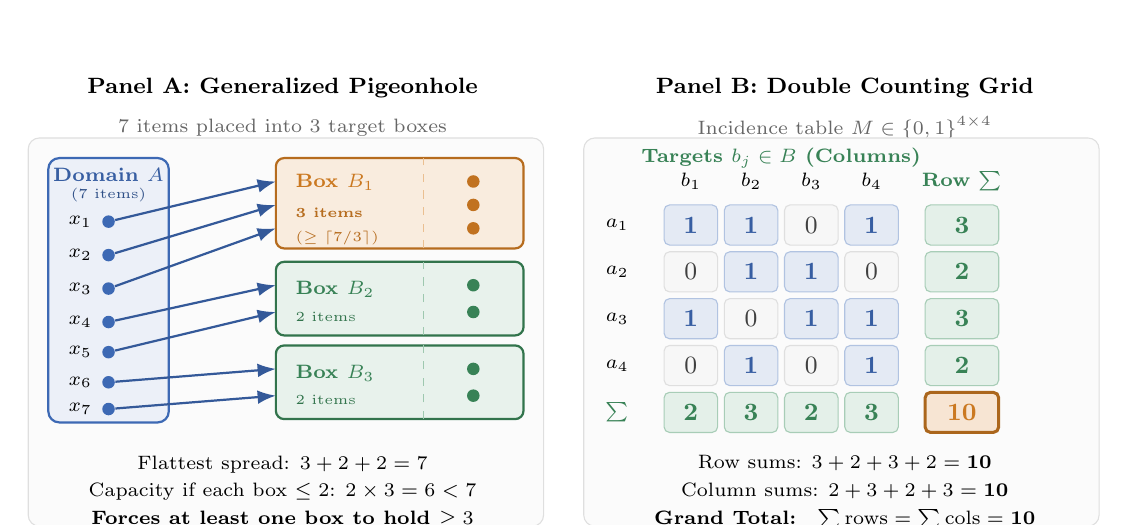
\begin{tikzpicture}[scale=0.85, >=Latex]
  % ==========================================
  % Panel A: Generalized Pigeonhole Principle
  % ==========================================
  \begin{scope}[xshift=0cm]
    \node[anchor=south, font=\footnotesize\bfseries] at (3.5, 5.0) {Panel A: Generalized Pigeonhole};
    \node[font=\scriptsize, text=gray!80!black] at (3.5, 4.7) {$7$ items placed into $3$ target boxes};
    \draw[rounded corners=4pt, fill=gray!3, draw=gray!25] (-0.3, -1.25) rectangle (7.4, 4.55);

    % Domain container A
    \draw[thick, sourceblue, fill=sourceblue!10, rounded corners=4pt] (0.0, 0.3) rectangle (1.8, 4.25);
    \node[sourceblue!90!black, font=\scriptsize\bfseries] at (0.9, 4.0) {Domain $A$};
    \node[sourceblue!75!black, font=\tiny] at (0.9, 3.7) {($7$ items)};

    % 7 Domain nodes
    \node[circle, fill=sourceblue, inner sep=1.6pt, label={left:\scriptsize $x_1$}] (x1) at (0.9, 3.30) {};
    \node[circle, fill=sourceblue, inner sep=1.6pt, label={left:\scriptsize $x_2$}] (x2) at (0.9, 2.80) {};
    \node[circle, fill=sourceblue, inner sep=1.6pt, label={left:\scriptsize $x_3$}] (x3) at (0.9, 2.30) {};
    \node[circle, fill=sourceblue, inner sep=1.6pt, label={left:\scriptsize $x_4$}] (x4) at (0.9, 1.80) {};
    \node[circle, fill=sourceblue, inner sep=1.6pt, label={left:\scriptsize $x_5$}] (x5) at (0.9, 1.35) {};
    \node[circle, fill=sourceblue, inner sep=1.6pt, label={left:\scriptsize $x_6$}] (x6) at (0.9, 0.90) {};
    \node[circle, fill=sourceblue, inner sep=1.6pt, label={left:\scriptsize $x_7$}] (x7) at (0.9, 0.50) {};

    % Box 1 (Overloaded, holds 3)
    \draw[thick, quotientorange!85!black, fill=quotientorange!15, rounded corners=3pt] (3.4, 2.9) rectangle (7.1, 4.25);
    \draw[quotientorange!50, dashed] (5.6, 2.9) -- (5.6, 4.25);
    \node[anchor=north west, font=\scriptsize\bfseries, quotientorange!95!black] at (3.55, 4.15) {Box $B_1$};
    \node[anchor=north west, font=\tiny\bfseries, quotientorange!85!black] at (3.55, 3.65) {$\mathbf{3}$ items};
    \node[anchor=north west, font=\tiny, quotientorange!85!black] at (3.55, 3.30) {($\ge \lceil 7/3 \rceil$)};
    % Tokens inside Box 1
    \node[circle, fill=quotientorange!90!black, inner sep=1.6pt] (t1) at (6.35, 3.90) {};
    \node[circle, fill=quotientorange!90!black, inner sep=1.6pt] (t2) at (6.35, 3.55) {};
    \node[circle, fill=quotientorange!90!black, inner sep=1.6pt] (t3) at (6.35, 3.20) {};

    % Box 2 (Holds 2)
    \draw[thick, targetgreen!80!black, fill=targetgreen!12, rounded corners=3pt] (3.4, 1.6) rectangle (7.1, 2.7);
    \draw[targetgreen!50, dashed] (5.6, 1.6) -- (5.6, 2.7);
    \node[anchor=north west, font=\scriptsize\bfseries, targetgreen!90!black] at (3.55, 2.55) {Box $B_2$};
    \node[anchor=north west, font=\tiny, targetgreen!80!black] at (3.55, 2.10) {$2$ items};
    % Tokens inside Box 2
    \node[circle, fill=targetgreen!90!black, inner sep=1.6pt] (t4) at (6.35, 2.35) {};
    \node[circle, fill=targetgreen!90!black, inner sep=1.6pt] (t5) at (6.35, 1.95) {};

    % Box 3 (Holds 2)
    \draw[thick, targetgreen!80!black, fill=targetgreen!12, rounded corners=3pt] (3.4, 0.35) rectangle (7.1, 1.45);
    \draw[targetgreen!50, dashed] (5.6, 0.35) -- (5.6, 1.45);
    \node[anchor=north west, font=\scriptsize\bfseries, targetgreen!90!black] at (3.55, 1.30) {Box $B_3$};
    \node[anchor=north west, font=\tiny, targetgreen!80!black] at (3.55, 0.85) {$2$ items};
    % Tokens inside Box 3
    \node[circle, fill=targetgreen!90!black, inner sep=1.6pt] (t6) at (6.35, 1.1) {};
    \node[circle, fill=targetgreen!90!black, inner sep=1.6pt] (t7) at (6.35, 0.7) {};

    % Mapping arrows
    \draw[->, thick, sourceblue!85!black] (x1) -- (3.4, 3.90);
    \draw[->, thick, sourceblue!85!black] (x2) -- (3.4, 3.55);
    \draw[->, thick, sourceblue!85!black] (x3) -- (3.4, 3.20);
    \draw[->, thick, sourceblue!85!black] (x4) -- (3.4, 2.35);
    \draw[->, thick, sourceblue!85!black] (x5) -- (3.4, 1.95);
    \draw[->, thick, sourceblue!85!black] (x6) -- (3.4, 1.10);
    \draw[->, thick, sourceblue!85!black] (x7) -- (3.4, 0.70);

    \node[below, font=\scriptsize, align=center] at (3.5, -0.05) {Flattest spread: $3 + 2 + 2 = 7$\\[2pt]Capacity if each box $\le 2$: $2 \times 3 = 6 < 7$\\[2pt]\textbf{Forces at least one box to hold $\ge 3$}};
  \end{scope}

  % ==========================================
  % Panel B: Double Counting Incidence Grid
  % ==========================================
  \begin{scope}[xshift=8.6cm]
    \node[anchor=south, font=\footnotesize\bfseries] at (3.3, 5.0) {Panel B: Double Counting Grid};
    \node[font=\scriptsize, text=gray!80!black] at (3.3, 4.7) {Incidence table $M \in \{0,1\}^{4 \times 4}$};
    \draw[rounded corners=4pt, fill=gray!3, draw=gray!25] (-0.6, -1.25) rectangle (7.1, 4.55);

    % Column headers
    \node[targetgreen!90!black, font=\scriptsize\bfseries] at (2.35, 4.25) {Targets $b_j \in B$ (Columns)};
    \node[font=\scriptsize\bfseries] at (1.0, 3.9) {$b_1$};
    \node[font=\scriptsize\bfseries] at (1.9, 3.9) {$b_2$};
    \node[font=\scriptsize\bfseries] at (2.8, 3.9) {$b_3$};
    \node[font=\scriptsize\bfseries] at (3.7, 3.9) {$b_4$};
    \node[targetgreen!90!black, font=\scriptsize\bfseries] at (5.05, 3.9) {Row $\sum$};

    % Row headers
    \node[font=\scriptsize\bfseries] at (-0.1, 3.25) {$a_1$};
    \node[font=\scriptsize\bfseries] at (-0.1, 2.55) {$a_2$};
    \node[font=\scriptsize\bfseries] at (-0.1, 1.85) {$a_3$};
    \node[font=\scriptsize\bfseries] at (-0.1, 1.15) {$a_4$};

    % Grid entries (Row 1): [1, 1, 0, 1] -> 3
    \draw[fill=sourceblue!14, draw=sourceblue!40, rounded corners=2pt] (0.6, 2.95) rectangle (1.4, 3.55);
    \node[sourceblue!90!black, font=\small\bfseries] at (1.0, 3.25) {1};
    \draw[fill=sourceblue!14, draw=sourceblue!40, rounded corners=2pt] (1.5, 2.95) rectangle (2.3, 3.55);
    \node[sourceblue!90!black, font=\small\bfseries] at (1.9, 3.25) {1};
    \draw[fill=gray!6, draw=gray!25, rounded corners=2pt] (2.4, 2.95) rectangle (3.2, 3.55);
    \node[gray!50!black, font=\small] at (2.8, 3.25) {0};
    \draw[fill=sourceblue!14, draw=sourceblue!40, rounded corners=2pt] (3.3, 2.95) rectangle (4.1, 3.55);
    \node[sourceblue!90!black, font=\small\bfseries] at (3.7, 3.25) {1};
    \draw[fill=targetgreen!14, draw=targetgreen!45, rounded corners=2pt] (4.5, 2.95) rectangle (5.6, 3.55);
    \node[targetgreen!90!black, font=\small\bfseries] at (5.05, 3.25) {3};

    % Grid entries (Row 2): [0, 1, 1, 0] -> 2
    \draw[fill=gray!6, draw=gray!25, rounded corners=2pt] (0.6, 2.25) rectangle (1.4, 2.85);
    \node[gray!50!black, font=\small] at (1.0, 2.55) {0};
    \draw[fill=sourceblue!14, draw=sourceblue!40, rounded corners=2pt] (1.5, 2.25) rectangle (2.3, 2.85);
    \node[sourceblue!90!black, font=\small\bfseries] at (1.9, 2.55) {1};
    \draw[fill=sourceblue!14, draw=sourceblue!40, rounded corners=2pt] (2.4, 2.25) rectangle (3.2, 2.85);
    \node[sourceblue!90!black, font=\small\bfseries] at (2.8, 2.55) {1};
    \draw[fill=gray!6, draw=gray!25, rounded corners=2pt] (3.3, 2.25) rectangle (4.1, 2.85);
    \node[gray!50!black, font=\small] at (3.7, 2.55) {0};
    \draw[fill=targetgreen!14, draw=targetgreen!45, rounded corners=2pt] (4.5, 2.25) rectangle (5.6, 2.85);
    \node[targetgreen!90!black, font=\small\bfseries] at (5.05, 2.55) {2};

    % Grid entries (Row 3): [1, 0, 1, 1] -> 3
    \draw[fill=sourceblue!14, draw=sourceblue!40, rounded corners=2pt] (0.6, 1.55) rectangle (1.4, 2.15);
    \node[sourceblue!90!black, font=\small\bfseries] at (1.0, 1.85) {1};
    \draw[fill=gray!6, draw=gray!25, rounded corners=2pt] (1.5, 1.55) rectangle (2.3, 2.15);
    \node[gray!50!black, font=\small] at (1.9, 1.85) {0};
    \draw[fill=sourceblue!14, draw=sourceblue!40, rounded corners=2pt] (2.4, 1.55) rectangle (3.2, 2.15);
    \node[sourceblue!90!black, font=\small\bfseries] at (2.8, 1.85) {1};
    \draw[fill=sourceblue!14, draw=sourceblue!40, rounded corners=2pt] (3.3, 1.55) rectangle (4.1, 2.15);
    \node[sourceblue!90!black, font=\small\bfseries] at (3.7, 1.85) {1};
    \draw[fill=targetgreen!14, draw=targetgreen!45, rounded corners=2pt] (4.5, 1.55) rectangle (5.6, 2.15);
    \node[targetgreen!90!black, font=\small\bfseries] at (5.05, 1.85) {3};

    % Grid entries (Row 4): [0, 1, 0, 1] -> 2
    \draw[fill=gray!6, draw=gray!25, rounded corners=2pt] (0.6, 0.85) rectangle (1.4, 1.45);
    \node[gray!50!black, font=\small] at (1.0, 1.15) {0};
    \draw[fill=sourceblue!14, draw=sourceblue!40, rounded corners=2pt] (1.5, 0.85) rectangle (2.3, 1.45);
    \node[sourceblue!90!black, font=\small\bfseries] at (1.9, 1.15) {1};
    \draw[fill=gray!6, draw=gray!25, rounded corners=2pt] (2.4, 0.85) rectangle (3.2, 1.45);
    \node[gray!50!black, font=\small] at (2.8, 1.15) {0};
    \draw[fill=sourceblue!14, draw=sourceblue!40, rounded corners=2pt] (3.3, 0.85) rectangle (4.1, 1.45);
    \node[sourceblue!90!black, font=\small\bfseries] at (3.7, 1.15) {1};
    \draw[fill=targetgreen!14, draw=targetgreen!45, rounded corners=2pt] (4.5, 0.85) rectangle (5.6, 1.45);
    \node[targetgreen!90!black, font=\small\bfseries] at (5.05, 1.15) {2};

    % Col sums (Row 5): [2, 3, 2, 3] and Grand Total
    \draw[fill=targetgreen!14, draw=targetgreen!45, rounded corners=2pt] (0.6, 0.15) rectangle (1.4, 0.75);
    \node[targetgreen!90!black, font=\small\bfseries] at (1.0, 0.45) {2};
    \draw[fill=targetgreen!14, draw=targetgreen!45, rounded corners=2pt] (1.5, 0.15) rectangle (2.3, 0.75);
    \node[targetgreen!90!black, font=\small\bfseries] at (1.9, 0.45) {3};
    \draw[fill=targetgreen!14, draw=targetgreen!45, rounded corners=2pt] (2.4, 0.15) rectangle (3.2, 0.75);
    \node[targetgreen!90!black, font=\small\bfseries] at (2.8, 0.45) {2};
    \draw[fill=targetgreen!14, draw=targetgreen!45, rounded corners=2pt] (3.3, 0.15) rectangle (4.1, 0.75);
    \node[targetgreen!90!black, font=\small\bfseries] at (3.7, 0.45) {3};

    % Col sum label on left
    \node[targetgreen!90!black, font=\scriptsize\bfseries] at (-0.1, 0.45) {$\sum$};

    % Grand total cell
    \draw[fill=quotientorange!20, draw=quotientorange!80!black, line width=1.1pt, rounded corners=2pt] (4.5, 0.15) rectangle (5.6, 0.75);
    \node[quotientorange!95!black, font=\small\bfseries] at (5.05, 0.45) {10};

    \node[below, font=\scriptsize, align=center] at (3.3, -0.05) {Row sums: $3 + 2 + 3 + 2 = \mathbf{10}$\\[2pt]Column sums: $2 + 3 + 2 + 3 = \mathbf{10}$\\[2pt]\textbf{Grand Total: } $\sum\text{rows} = \sum\text{cols} = \mathbf{10}$};
  \end{scope}
\end{tikzpicture}
\caption{The two workhorses of finite mapping theory. \textbf{Left}: The Generalized Pigeonhole Principle with $7$ items placed into $3$ boxes. Even the most uniform partition ($3, 2, 2$) forces at least one box to contain $\ge \lceil 7/3 \rceil = 3$ items. \textbf{Right}: Double counting on an incidence matrix $M \in \{0,1\}^{4 \times 4}$. Summing horizontally along rows or vertically down columns yields the exact same total: $\sum_{a} \text{row}(a) = \sum_{b} \text{col}(b) = 10$.}
\label{13:fig-pigeonhole-doublecount}
\end{figure}

The true craft of using the Pigeonhole Principle lies in choosing the pigeonholes. In most non-trivial applications, the boxes are not presented in advance; you must construct them from the underlying mathematical structure.

\begin{example}[Differences Divisible by $n$]
Let $n \in \N$ and let $S \subset \Z$ be any collection of $n+1$ distinct integers. Prove that there exist two distinct integers $x, y \in S$ whose difference $x - y$ is a multiple of $n$.

\textbf{Proof.}
By the division algorithm, dividing any integer by $n$ yields a remainder in the set:
\[
R = \{0, 1, 2, \dots, n-1\}.
\]
The set $R$ contains exactly $n$ possible remainders. These $n$ remainders are our pigeonholes.

Define the mapping $f: S \to R$ by $f(z) = z \bmod n$. The domain $S$ contains $n+1$ elements (the pigeons), while the codomain $R$ contains $n$ elements (the pigeonholes). 

Because $|S| = n + 1 > n = |R|$, the function $f$ cannot be injective. There exist distinct elements $x, y \in S$ such that $f(x) = f(y)$. Hence $x$ and $y$ share the exact same remainder $r \in R$:
\[
x = q_1 n + r \quad \text{and} \quad y = q_2 n + r \quad \text{for some } q_1, q_2 \in \Z.
\]
Subtracting the two expressions:
\[
x - y = (q_1 n + r) - (q_2 n + r) = (q_1 - q_2)n.
\]
Since $q_1 - q_2$ is an integer, $x - y$ is an exact multiple of $n$. 

To see this in action, pick $n = 5$ and choose $6$ arbitrary integers: $S = \{14, 23, 37, 51, 69, 93\}$. Computing each remainder modulo $5$:
\[
14 \equiv 4, \quad 23 \equiv 3, \quad 37 \equiv 2, \quad 51 \equiv 1, \quad 69 \equiv 4, \quad 93 \equiv 3 \pmod 5.
\]
Both $14$ and $69$ land in remainder box $4$; their difference $69 - 14 = 55 = 5 \times 11$ is a multiple of $5$. Both $23$ and $93$ land in remainder box $3$; their difference $93 - 23 = 70 = 5 \times 14$ is also a multiple of $5$. The collision was guaranteed before inspecting a single digit.
\end{example}

\begin{example}[Points in a $2 \times 2$ Square]
Suppose $5$ points are placed inside a $2 \times 2$ square $Q = [0, 2] \times [0, 2]$ in the plane. Prove that at least two of the points must lie within a Euclidean distance of at most $\sqrt{2}$ of each other.

\textbf{Proof.}
We partition the continuous $2 \times 2$ square into four $1 \times 1$ sub-squares:
\[
Q_1 = [0, 1] \times [0, 1], \quad Q_2 = [1, 2] \times [0, 1], \quad Q_3 = [0, 1] \times [1, 2], \quad Q_4 = [1, 2] \times [1, 2].
\]
If a point lies on an internal boundary shared by multiple sub-squares, assign it to any one of the adjacent squares arbitrarily. 

We have $5$ points and $4$ sub-squares. By the Pigeonhole Principle, at least one sub-square $Q_k$ must contain at least $\lceil 5/4 \rceil = 2$ points. Let these two points be $P_1 = (x_1, y_1)$ and $P_2 = (x_2, y_2)$.

Because both points lie inside the same $1 \times 1$ square $Q_k$, their horizontal and vertical coordinate separations are bounded:
\[
|x_1 - x_2| \le 1 \qquad \text{and} \qquad |y_1 - y_2| \le 1.
\]
The Euclidean distance $d(P_1, P_2)$ between them is bounded by the diagonal of the unit square:
\[
d(P_1, P_2) = \sqrt{(x_1 - x_2)^2 + (y_1 - y_2)^2} \le \sqrt{1^2 + 1^2} = \sqrt{2} \approx 1.414.
\]
Observe the geometric constraint at work: even if an adversary places the first four points at the extreme outer corners $(0,0), (2,0), (0,2), (2,2)$---maximizing their separations to $2$ and $2\sqrt{2}$---the fifth point cannot escape. Wherever it is placed, it enters a quadrant already containing a corner point, forcing a separation of at most $\sqrt{2}$.
\end{example}

\subsubsection{Double Counting: Counting a 0--1 Grid by Rows vs. by Columns}

A bijection proves that $|A| = |B|$ by building a one-to-one correspondence between two sets. But what if we wish to establish an equality between two complicated combinatorial formulas where an explicit element-by-element matching is elusive?

The technique of \textbf{Double Counting} (or two-way counting) provides the answer. Instead of matching elements directly, we count the size of a single set of relational pairs in two distinct ways.

Let $A$ and $B$ be finite sets, and let $R \subseteq A \times B$ be a relation between them. We encode $R$ as an \emph{incidence matrix} $M \in \{0, 1\}^{|A| \times |B|}$, where each entry indicates whether a pair belongs to $R$:
\[
M_{a, b} = \begin{cases} 1 & \text{if } (a, b) \in R, \\ 0 & \text{if } (a, b) \notin R. \end{cases}
\]
Now ask a simple question: \emph{How many total $1$s are present in the table?}

We can tally the total sum $S$ in two legitimate ways:
\begin{enumerate}
\item \textbf{Row by Row (Horizontal Sum):} Sum the entries across each row first, obtaining the row total $\text{row}(a) = \sum_{b \in B} M_{a, b}$, and then add all row totals together:
\[
S = \sum_{a \in A} \text{row}(a) = \sum_{a \in A} \left( \sum_{b \in B} M_{a, b} \right).
\]
\item \textbf{Column by Column (Vertical Sum):} Sum the entries down each column first, obtaining the column total $\text{col}(b) = \sum_{a \in A} M_{a, b}$, and then add all column totals together:
\[
S = \sum_{b \in B} \text{col}(b) = \sum_{b \in B} \left( \sum_{a \in A} M_{a, b} \right).
\]
\end{enumerate}
Because finite addition is commutative and associative, changing the order of summation leaves the grand total unchanged. We obtain the universal identity:
\[
\sum_{a \in A} \text{row}(a) = \sum_{b \in B} \text{col}(b).
\]
This identity is illustrated in Figure~\ref{13:fig-pigeonhole-doublecount}, Panel~B: summing the rows yields $3 + 2 + 3 + 2 = 10$, and summing the columns yields $2 + 3 + 2 + 3 = 10$. Both roads arrive at the same destination.

\begin{example}[Euler's Handshake Lemma]
In any finite graph $G = (V, E)$, the sum of the degrees of all vertices equals twice the number of edges:
\[
\sum_{v \in V} \deg(v) = 2|E|.
\]

\textbf{Proof.}
Construct an incidence table where rows correspond to vertices $v \in V$ and columns correspond to edges $e \in E$. Set the cell entry to $1$ if vertex $v$ is an endpoint of edge $e$, and $0$ otherwise:
\[
M_{v, e} = \begin{cases} 1 & \text{if } v \in e, \\ 0 & \text{if } v \notin e. \end{cases}
\]
We evaluate the total number of $1$s in $M$ in two ways:
\begin{itemize}
\item \textbf{Summing across rows:} For a fixed vertex $v$, the row sum counts how many edges have $v$ as an endpoint. By definition, this is the degree $\deg(v)$. Summing across all vertices gives $\sum_{v \in V} \deg(v)$.
\item \textbf{Summing down columns:} For a fixed edge $e = \{u, w\}$, the edge connects exactly $2$ endpoints. Thus every single column contains exactly two $1$s. Summing across all $|E|$ edges gives $\sum_{e \in E} 2 = 2|E|$.
\end{itemize}
Equating both expressions yields $\sum_{v \in V} \deg(v) = 2|E|$. 

An immediate structural consequence follows: because $2|E|$ is an even integer, the sum of all vertex degrees must be even. Hence, the number of vertices with odd degree must be even (at any gathering, the number of people who have shaken hands an odd number of times is always even).
\end{example}

\begin{example}[Counting Committee-Chair Pairs]
Let $n, k \in \N$ with $1 \le k \le n$. Prove combinatorially that:
\[
k \binom{n}{k} = n \binom{n-1}{k-1}.
\]

\textbf{Proof.}
Rather than expanding into factorials $\frac{n!}{(k-1)!(n-k)!}$ and canceling terms algebraically, we count a single set in two ways.

Suppose from a pool of $n$ people, we want to form a committee of $k$ members, and from within that committee, select one person to serve as chair. Define the set of valid configurations:
\[
\mathcal{S} = \{(C, p) : C \subseteq P, \, |C| = k, \, p \in C\},
\]
where $P$ is the population of $n$ people, $C$ is a committee of size $k$, and $p \in C$ is the designated chair. We compute $|\mathcal{S}|$ from two viewpoints:
\begin{itemize}
\item \textbf{Viewpoint 1 (Choose committee first, then select chair):}
There are $\binom{n}{k}$ ways to choose the committee $C$ of size $k$ from the $n$ candidates. Once $C$ is fixed, there are $k$ choices for which committee member serves as chair $p$. The number of pairs is:
\[
|\mathcal{S}| = \binom{n}{k} \times k = k \binom{n}{k}.
\]
\item \textbf{Viewpoint 2 (Choose chair first, then fill remaining seats):}
There are $n$ ways to select the chair $p$ from the entire pool of $n$ people. Once the chair is established, the remaining $k-1$ committee members must be selected from the remaining $n-1$ available candidates. This can be done in $\binom{n-1}{k-1}$ ways. The number of pairs is:
\[
|\mathcal{S}| = n \times \binom{n-1}{k-1} = n \binom{n-1}{k-1}.
\]
\end{itemize}
Both viewpoints count the exact same set $\mathcal{S}$ of chair-committee pairs. Therefore, the two expressions must be equal:
\[
k \binom{n}{k} = n \binom{n-1}{k-1}.
\]
Double counting transforms an algebraic manipulation into a structural story about perspectives on a single set.
\end{example}

\subsection{What Mapping Theory Unlocked, Its Honest Limits, and Where We Go Next}

Classifying functions into injections, surjections, and bijections provides the rigorous scaffolding for all of higher mathematics. It gives us:
\begin{itemize}
\item \textbf{Invertibility without guessing:} A function has a two-way inverse if and only if it is a bijection. You no longer have to guess whether an equation can be reversed; checking injectivity and surjectivity decides the matter definitively.
\item \textbf{Isomorphisms:} In abstract algebra (Chapter~21), two groups or vector spaces that look completely different on the surface are recognized as fundamentally identical if there exists a structure-preserving bijection between them.
\item \textbf{Measuring the infinite:} In Chapter~19, we will use bijections to discover the astounding fact that while the integers and rational numbers share the same cardinality ($\aleph_0$), the real numbers form a strictly larger infinity that no bijection can reach.
\end{itemize}

Yet we must acknowledge the honest limitation of this framework: injectivity and surjectivity are strictly \textbf{pointwise} concepts. They inspect single inputs $a$ and single outputs $b$ in isolation. 

In geometry, calculus, and topology, however, spaces are rarely understood one lonely point at a time. We need to know how a mapping stretches, tears, folds, or preserves whole geometric regions, open disks, and continuous curves. If you try to analyze a continuous wave or a gravitational field by tracking every individual point, the notation collapses into chaos.

To understand how functions act on whole collections of points simultaneously, we need to lift our machinery from elements to subsets. In Chapter~14, we study \textbf{Images and Inverse Images}, discovering that pulling backward across a function (preimages) preserves the algebraic fabric of sets in ways that pushing forward can never match.

\subsection{Exercises}

\begin{enumerate}
\item For each function, determine whether it is injective, surjective, or bijective. Provide rigorous proofs or explicit counterexamples:
\begin{enumerate}[label=(\alph*)]
\item $f: \Z \to \Z$ defined by $f(n) = 2n + 3$.
\item $g: \Q \to \Q$ defined by $g(x) = 2x + 3$.
\item $h: \R \to \R$ defined by $h(x) = x^3 - x$.
\end{enumerate}
\item Let $f: A \to B$ and $g: B \to C$ be functions. Prove that if both $f$ and $g$ are injective, their composition $g \circ f: A \to C$ is injective.
\item Prove that if $g \circ f$ is surjective, then $g$ must be surjective. Must $f$ also be surjective? Provide a proof or counterexample.
\item Suppose $n+1$ distinct integers are chosen from the set $\{1, 2, \dots, 2n\}$. Prove that there exist two chosen integers such that one divides the other. (\emph{Hint:} Write each chosen integer in the form $2^k \cdot m$, where $m$ is an odd integer, and identify the pigeonholes.)
\item Use double counting to prove the identity $\sum_{k=1}^n k = \binom{n+1}{2}$ by counting pairs of integers $\{x, y\} \subseteq \{1, 2, \dots, n+1\}$ with $x < y$, grouped by the value of the larger element $y$.
\end{enumerate}

\newpage

\section{Images and Inverse Images}
\chapterline

Up to this point, we have watched functions act on individual points: you feed an input $x$ into the machine, and an output $f(x)$ emerges on the other side. 

In higher mathematics, however, functions rarely operate one particle at a time. They act on entire regions, subspaces, and collections. A function $f: X \to Y$ creates a two-way transportation network between the subsets of $X$ and the subsets of $Y$:
\begin{itemize}
\item \textbf{Pushing Forward (Image):} Take a subset $S \subseteq X$ and transport it forward into $Y$ by collecting all outputs $f(s)$.
\item \textbf{Pulling Backward (Inverse Image / Preimage):} Select a target region $T \subseteq Y$ and trace backward to collect all points in $X$ whose outputs land in $T$.
\end{itemize}

At first glance, you might expect pushing forward and pulling backward to be mirror images of each other. But a deep asymmetry lives here: \emph{pulling backward behaves dramatically better than pushing forward}. Preimages preserve unions, intersections, and complements perfectly. Forward images, by contrast, can fracture and lose information whenever a function merges distinct inputs.

\begin{historybox}
This profound algebraic asymmetry was uncovered in the early twentieth century by Felix Hausdorff (\emph{Grundz\"uge der Mengenlehre}, 1914) alongside pioneers of the Polish and French schools of analysis (Maurice Fr\'echet, Kazimierz Kuratowski, and Henri Lebesgue). 

Mathematicians were trying to liberate calculus from the rigid confines of Euclidean $\R^n$. In abstract spaces where there are no coordinates, no rulers, and no $\eps$-$\delta$ formulas, how can one define whether a transformation is ``continuous'' or whether a region is ``measurable''? 

The early naive instinct was to push sets forward: if $U$ is an open neighborhood, shouldn't its image $f(U)$ also be open? But that approach collapsed immediately into counterexamples. Hausdorff realized that the true invariant structure of mathematics flows backward: the inverse image operation $f^{-1}$ is an exact Boolean algebra homomorphism. It preserves arbitrary unions, intersections, and complements without exception. This single algebraic discovery crowned the preimage as the primary structural engine for modern topology, measure theory, and modern analysis.
\end{historybox}

\subsection{Formal Definitions}

\begin{definition}[Forward Image]
Let $f: X \to Y$ be a function and let $S \subseteq X$. The \textbf{image} of $S$ under $f$ is
\[
f(S) = \{f(s) \in Y : s \in S\} = \{y \in Y : (\exists s \in S)(f(s) = y)\}.
\]
\end{definition}

\begin{definition}[Inverse Image / Preimage]
Let $f: X \to Y$ be a function and let $T \subseteq Y$. The \textbf{inverse image} (or \textbf{preimage}) of $T$ under $f$ is
\[
f^{-1}(T) = \{x \in X : f(x) \in T\}.
\]
\end{definition}

\begin{center}
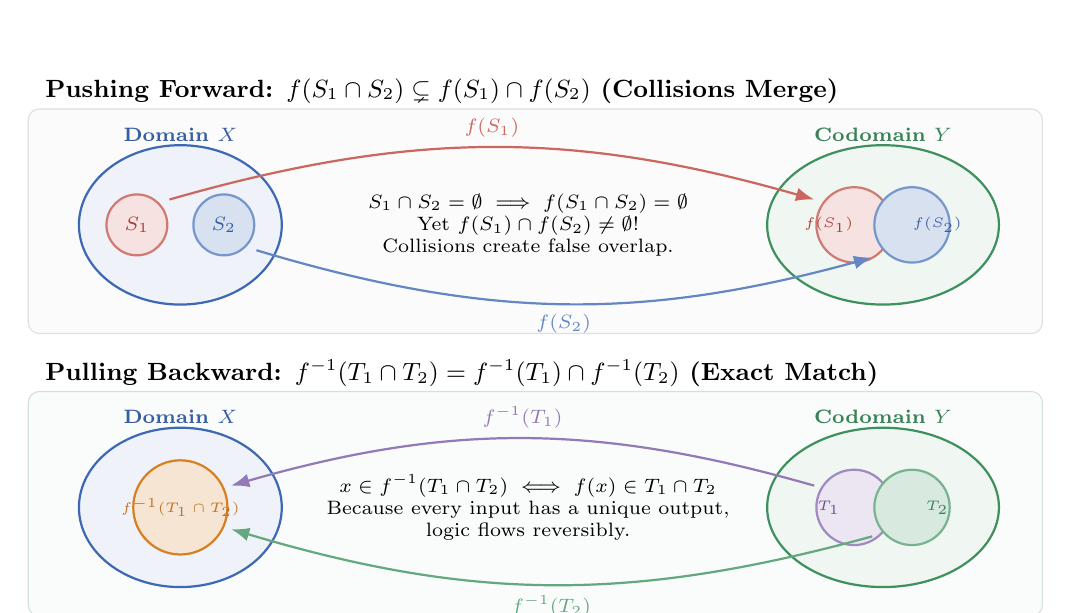
\begin{tikzpicture}[scale=0.92, >=Latex]
  % Panel 1: Forward Push with Information Loss
  \begin{scope}[yshift=0cm]
    \node[anchor=west, font=\small\bfseries] at (-0.5, 2.75) {Pushing Forward: $f(S_1 \cap S_2) \subsetneq f(S_1) \cap f(S_2)$ (Collisions Merge)};
    \draw[rounded corners=4pt, fill=gray!3, draw=gray!25] (-0.6, -0.6) rectangle (13.4, 2.5);
    
    % Domain X
    \draw[thick, sourceblue, fill=sourceblue!8] (1.5, 0.9) ellipse (1.4cm and 1.1cm);
    \node[sourceblue!90!black, font=\scriptsize\bfseries] at (1.5, 2.15) {Domain $X$};
    
    % Disjoint sets S1 and S2
    \draw[thick, trapred!70, fill=trapred!15] (0.9, 0.9) circle (0.42cm);
    \node[trapred!90!black, font=\scriptsize\bfseries] at (0.9, 0.9) {$S_1$};
    \draw[thick, sourceblue!70, fill=sourceblue!20] (2.1, 0.9) circle (0.42cm);
    \node[sourceblue!90!black, font=\scriptsize\bfseries] at (2.1, 0.9) {$S_2$};
    
    % Codomain Y
    \draw[thick, targetgreen, fill=targetgreen!8] (11.2, 0.9) ellipse (1.6cm and 1.1cm);
    \node[targetgreen!90!black, font=\scriptsize\bfseries] at (11.2, 2.15) {Codomain $Y$};
    
    % Overlapping images
    \draw[thick, trapred!70, fill=trapred!15] (10.8, 0.9) circle (0.52cm);
    \draw[thick, sourceblue!70, fill=sourceblue!20] (11.6, 0.9) circle (0.52cm);
    \node[trapred!90!black, font=\tiny\bfseries] at (10.45, 0.9) {$f(S_1)$};
    \node[sourceblue!90!black, font=\tiny\bfseries] at (11.95, 0.9) {$f(S_2)$};
    
    % Arrows
    \draw[->, thick, trapred!80] (1.35, 1.25) to[bend left=16] node[above, font=\scriptsize] {$f(S_1)$} (10.25, 1.25);
    \draw[->, thick, sourceblue!80] (2.55, 0.55) to[bend right=16] node[below, font=\scriptsize] {$f(S_2)$} (11.05, 0.45);
    
    \node[anchor=center, font=\scriptsize, align=center] at (6.3, 0.9) {
      $S_1 \cap S_2 = \emptyset \implies f(S_1 \cap S_2) = \emptyset$\\
      Yet $f(S_1) \cap f(S_2) \neq \emptyset$!\\
      Collisions create false overlap.
    };
  \end{scope}

  % Panel 2: Pulling Backward Preserves Structure
  \begin{scope}[yshift=-3.9cm]
    \node[anchor=west, font=\small\bfseries] at (-0.5, 2.75) {Pulling Backward: $f^{-1}(T_1 \cap T_2) = f^{-1}(T_1) \cap f^{-1}(T_2)$ (Exact Match)};
    \draw[rounded corners=4pt, fill=targetgreen!3, draw=targetgreen!25] (-0.6, -0.6) rectangle (13.4, 2.5);
    
    % Domain X
    \draw[thick, sourceblue, fill=sourceblue!8] (1.5, 0.9) ellipse (1.4cm and 1.1cm);
    \node[sourceblue!90!black, font=\scriptsize\bfseries] at (1.5, 2.15) {Domain $X$};
    
    \draw[thick, quotientorange, fill=quotientorange!20] (1.5, 0.9) circle (0.65cm);
    \node[quotientorange!90!black, font=\tiny\bfseries] at (1.5, 0.9) {$f^{-1}(T_1 \cap T_2)$};
    
    % Codomain Y
    \draw[thick, targetgreen, fill=targetgreen!8] (11.2, 0.9) ellipse (1.6cm and 1.1cm);
    \node[targetgreen!90!black, font=\scriptsize\bfseries] at (11.2, 2.15) {Codomain $Y$};
    
    % Overlapping T1 and T2
    \draw[thick, structurepurple!70, fill=structurepurple!15] (10.8, 0.9) circle (0.52cm);
    \draw[thick, targetgreen!70, fill=targetgreen!20] (11.6, 0.9) circle (0.52cm);
    \node[structurepurple!90!black, font=\tiny\bfseries] at (10.45, 0.9) {$T_1$};
    \node[targetgreen!90!black, font=\tiny\bfseries] at (11.95, 0.9) {$T_2$};
    
    % Reverse arrows
    \draw[<-, thick, structurepurple!80] (2.2, 1.2) to[bend left=16] node[above, font=\scriptsize] {$f^{-1}(T_1)$} (10.25, 1.2);
    \draw[<-, thick, targetgreen!80] (2.2, 0.6) to[bend right=16] node[below, font=\scriptsize] {$f^{-1}(T_2)$} (11.05, 0.5);
    
    \node[anchor=center, font=\scriptsize, align=center] at (6.3, 0.9) {
      $x \in f^{-1}(T_1 \cap T_2) \iff f(x) \in T_1 \cap T_2$\\
      Because every input has a unique output,\\
      logic flows reversibly.
    };
  \end{scope}
\end{tikzpicture}
\end{center}

\begin{trapbox}
The symbol $f^{-1}(T)$ represents a set-theoretic operation on subsets of the codomain. It exists for \textbf{every} function $f$, whether or not $f$ is invertible! If $f(x) = x^2$, the inverse function $f^{-1}: \R \to \R$ does not exist, yet $f^{-1}([1, 4]) = [-2, -1] \cup [1, 2]$ is a perfectly well-defined subset of $\R$.
\end{trapbox}

\subsection{Why Preimages Behave So Beautifully}

To understand why preimages preserve set operations without exception, notice that determining whether $x \in f^{-1}(T)$ comes down to evaluating a single output: does $f(x)$ land inside $T$?

Because $f$ is a function, every element $x$ has exactly one output $f(x)$. There is no ambiguity. The point $f(x)$ either belongs to an intersection, union, or complement, or it does not.

\begin{theorem}[Preimages Distribute Over Intersections]
Let $f: X \to Y$ be a function and let $T_1, T_2 \subseteq Y$. Then
\[
f^{-1}(T_1 \cap T_2) = f^{-1}(T_1) \cap f^{-1}(T_2).
\]
\end{theorem}

\begin{proof}
Let $x \in X$ be arbitrary. We trace the logical biconditionals:
\begin{align*}
x \in f^{-1}(T_1 \cap T_2) 
&\iff f(x) \in T_1 \cap T_2 && \text{(definition of preimage)} \\
&\iff f(x) \in T_1 \text{ and } f(x) \in T_2 && \text{(definition of intersection)} \\
&\iff x \in f^{-1}(T_1) \text{ and } x \in f^{-1}(T_2) && \text{(definition of preimage)} \\
&\iff x \in f^{-1}(T_1) \cap f^{-1}(T_2) && \text{(definition of intersection)}.
\end{align*}
Since each step is an equivalence, the two sets contain identical elements:
\[
f^{-1}(T_1 \cap T_2) = f^{-1}(T_1) \cap f^{-1}(T_2). \qedhere
\]
\end{proof}

The identical argument works for unions and complements:
\[
f^{-1}(T_1 \cup T_2) = f^{-1}(T_1) \cup f^{-1}(T_2), \qquad f^{-1}(Y \setminus T) = X \setminus f^{-1}(T).
\]
The preimage is an algebraic homomorphism on Boolean algebras: it commutes with every standard set operation.

\subsection{Where Forward Images Break Down}

Now contrast this with the forward image of an intersection:

\begin{theorem}
Let $f: X \to Y$ and let $S_1, S_2 \subseteq X$. Then
\[
f(S_1 \cap S_2) \subseteq f(S_1) \cap f(S_2).
\]
\end{theorem}

\begin{proof}
Let $y \in f(S_1 \cap S_2)$ be arbitrary. By definition of the forward image, there exists some $x \in S_1 \cap S_2$ such that $f(x) = y$.

Since $x \in S_1 \cap S_2$, we have $x \in S_1$ and $x \in S_2$.
\begin{itemize}
\item Because $x \in S_1$ and $f(x) = y$, we have $y \in f(S_1)$.
\item Because $x \in S_2$ and $f(x) = y$, we have $y \in f(S_2)$.
\end{itemize}
Thus $y \in f(S_1) \cap f(S_2)$. Hence $f(S_1 \cap S_2) \subseteq f(S_1) \cap f(S_2)$.
\end{proof}

\emph{Why does the reverse inclusion fail?} 
Suppose $y \in f(S_1) \cap f(S_2)$. This means $y \in f(S_1)$ and $y \in f(S_2)$.
Therefore, there exists some $x_1 \in S_1$ with $f(x_1) = y$, and there exists some $x_2 \in S_2$ with $f(x_2) = y$.
\emph{Does this guarantee $x_1 = x_2$?}

No! If $f$ is not injective, $x_1$ and $x_2$ could be two completely different inputs that happen to collide on the same destination $y$. If $x_1 \neq x_2$, neither element needs to live in the intersection $S_1 \cap S_2$, leaving $f(S_1 \cap S_2)$ empty even though $f(S_1) \cap f(S_2)$ is non-empty!

\begin{example}[A Clean Counterexample]
Let $f: \R \to \R$ be $f(x) = x^2$.
Take the disjoint subsets $S_1 = \{-2\}$ and $S_2 = \{2\}$.
Their intersection is empty: $S_1 \cap S_2 = \emptyset$, so
\[
f(S_1 \cap S_2) = f(\emptyset) = \emptyset.
\]
However, computing the images separately:
\[
f(S_1) = \{4\}, \qquad f(S_2) = \{4\}, \implies f(S_1) \cap f(S_2) = \{4\}.
\]
Here $\emptyset \subsetneq \{4\}$. The equality fails precisely because $-2$ and $2$ collided under the squaring map.
\end{example}

\begin{theorem}
The equality $f(S_1 \cap S_2) = f(S_1) \cap f(S_2)$ holds for all subsets $S_1, S_2 \subseteq X$ if and only if $f$ is injective.
\end{theorem}

\subsection{Why Mathematicians Care: The Gateway to Topology}

This structural superiority of the preimage is the reason modern topology defines \emph{continuous functions} via inverse images:
\begin{center}
\emph{A function $f: X \to Y$ is continuous if for every open set $V \subseteq Y$, the preimage $f^{-1}(V)$ is open in $X$.}
\end{center}
If topologists had tried to define continuity using forward images (requiring $f(U)$ to be open whenever $U$ is open), even standard, smoothly behaving functions like $f(x) = x^2$ would fail: the open interval $(-1, 1)$ maps to $[0, 1)$, which includes its boundary point $0$ and is not open in $\R$! Preimages preserve topological structure without distortion, while forward images routinely fold and collapse boundary boundaries.

\subsection{What Preimages Unlocked, Their Limits, and Where We Go Next}

Mastering set transport unlocked the architecture of modern pure mathematics:
\begin{itemize}
\item \textbf{Topology without coordinates:} Defining continuity via $f^{-1}(V)$ (Chapter~22) allows us to study curved spaces, infinite-dimensional function spaces, and manifolds without ever drawing an $x$-$y$ axis.
\item \textbf{Measure theory and probability:} In rigorous probability, a random variable $X$ is not a mystery number; it is a measurable function, and the probability of an event $E$ is evaluated by pulling $E$ backward into the sample space: $\P(X \in E) = \P(X^{-1}(E))$.
\item \textbf{Algebraic pullbacks:} Dual spaces, differential forms, and bundle projections all rely on preimages to pull structures back from target spaces into source spaces.
\end{itemize}

Yet image and preimage operations have an inherent boundary: they are \textbf{transport mechanisms between two pre-existing spaces} $X$ and $Y$. They take sets that already exist in one world and ship them to another. 

What they cannot do is manufacture a \emph{new} mathematical universe out of an existing one. They cannot take a single space $X$ and simplify it from within—identifying points that are redundant, collapsing symmetries, or gluing opposite edges of a square together to create a cylinder or a donut.

To forge new spaces by collapsing redundant information, we need an entirely different kind of mathematical engine. In Chapter~15, we introduce \textbf{Relations and Equivalence}, discovering how the three axioms of equivalence allow us to quotient spaces and build new mathematical objects from the ground up.

\subsection{Exercises}

\begin{enumerate}
\item Let $f: X \to Y$ and let $S \subseteq X$ and $T \subseteq Y$.
\begin{enumerate}[label=(\alph*)]
\item Prove that $S \subseteq f^{-1}(f(S))$. Give a concrete example where equality fails.
\item Prove that $f(f^{-1}(T)) \subseteq T$. Give a concrete example where equality fails.
\end{enumerate}
\item Prove that $f^{-1}(T_1 \cup T_2) = f^{-1}(T_1) \cup f^{-1}(T_2)$ for any $T_1, T_2 \subseteq Y$.
\item Prove that $f(S_1 \cup S_2) = f(S_1) \cup f(S_2)$ for any $S_1, S_2 \subseteq X$. Why does union preserve equality for forward images while intersection does not?
\item Let $f: \R \to \R$ be defined by $f(x) = x^2 - 2x$. Find:
\begin{enumerate}[label=(\alph*)]
\item $f([0, 3])$.
\item $f^{-1}([-1, 3])$.
\item $f^{-1}(\{-5\})$.
\end{enumerate}
\end{enumerate}

\newpage

\section{Relations and Equivalence}
\chapterline

In everyday life, we constantly decide that two different things are ``the same'' for a specific purpose. 

A one-dollar bill printed in 2017 and a crisp bill printed in 2024 are made of different atoms and carry different serial numbers. But if you buy a coffee, the cashier does not inspect the serial numbers. For the purpose of commerce, both bills are identical.

Similarly, on an analog clock, the numbers $1$, $13$, and $25$ represent entirely different quantities of hours. Yet when reading the hour hand, all three point to the exact same position on the dial. The differences of $12$ hours have been deliberately collapsed.

In mathematics, the tool that formalizes this act of purposeful simplification is the \textbf{equivalence relation}.

\begin{historybox}
The conceptual origin of equivalence relations traces directly to a young Carl Friedrich Gauss. In his 1801 masterpiece, \emph{Disquisitiones Arithmeticae}, the 24-year-old Gauss revolutionized number theory by introducing modular arithmetic and the congruence symbol $a \equiv b \pmod n$. 

Before Gauss, mathematicians treated remainders as awkward numerical byproducts of Euclidean division. When dividing $17$ by $5$, the remainder $2$ was merely what was left over. Gauss made an extraordinary conceptual leap: numbers that leave the same remainder modulo $n$ should not be treated as separate integers with an incidental shared feature. They should be recognized as members of a single, unified mathematical organism: an \emph{equivalence class}.

Contemporaries initially balked at Gauss's new notation, asking why one could not simply write the equation $a - b = k n$. Gauss understood that the notation $\equiv$ reflected a profound structural reality: congruence behaves exactly like equality. It allows one to perform arithmetic on the classes themselves: $[a] + [b] = [a+b]$ and $[a][b] = [ab]$. 

Over the next century, mathematicians like Richard Dedekind, Henri Poincar\'e, and Emmy Noether realized that Gauss's construction was not unique to integers. It was the universal blueprint for manufacturing new spaces in geometry and abstract algebra: whenever you want to ignore extraneous details, factor out a symmetry, or glue geometric boundaries together, you define an equivalence relation and pass to the quotient.
\end{historybox}

\subsection{Relations in General}

Before studying equivalence, we need the general concept of a relation between elements of a set.

\begin{definition}[Relation]
A \textbf{binary relation} $R$ on a set $A$ is a subset of the Cartesian product:
\[
R \subseteq A \times A.
\]
If $(a, b) \in R$, we write $a \sim b$ or $a \, R \, b$, and say that ``$a$ is related to $b$.''
\end{definition}

A relation simply declares which pairs of elements are linked. Examples include:
\begin{itemize}
\item Arithmetic orders: $x < y$ or $x \le y$ on $\R$.
\item Divisibility: $a \mid b$ on the integers $\Z$.
\item Geometric connectivity: two points in a space connected by a continuous path.
\item Set containment: $S \subseteq T$ on the power set $\pow(U)$.
\end{itemize}

\subsection{The Three Axioms of Equivalence}

To behave like an idealized equality, a relation must satisfy three essential structural axioms.

\begin{definition}[Equivalence Relation]
A relation $\sim$ on a set $A$ is an \textbf{equivalence relation} if it satisfies:
\begin{enumerate}[label=(\roman*)]
\item \textbf{Reflexivity:} For all $a \in A$,
\[
a \sim a.
\]
(Every object is related to itself.)
\item \textbf{Symmetry:} For all $a, b \in A$,
\[
a \sim b \implies b \sim a.
\]
(The relation is two-way; perspective does not matter.)
\item \textbf{Transitivity:} For all $a, b, c \in A$,
\[
(a \sim b \text{ and } b \sim c) \implies a \sim c.
\]
(Chains of relation do not break.)
\end{enumerate}
\end{definition}

\begin{intuitionbox}
Think of reflexivity as self-recognition, symmetry as mutual agreement, and transitivity as contagion. Transitivity is the engine that prevents the world from fragmenting: if $a$ belongs to the same club as $b$, and $b$ belongs to the same club as $c$, then $a$ and $c$ must share membership in that club.
\end{intuitionbox}

\begin{trapbox}
\textbf{The Trap of Naive Similarity:}
It is tempting to think that any intuitive notion of ``being similar'' defines an equivalence relation. Consider the relation on $\R$ defined by $|x - y| \le 1$ (``$x$ and $y$ are within distance 1 of each other''). 
Reflexivity holds ($|x - x| = 0 \le 1$), and symmetry holds ($|y - x| = |x - y| \le 1$). 
Yet transitivity fails completely: $0 \sim 0.8$ and $0.8 \sim 1.5$, but $|0 - 1.5| = 1.5 > 1$, so $0 \not\sim 1.5$!
Without transitivity, elements cannot be partitioned into disjoint, non-overlapping islands. Similarity bleeds across boundaries; only true equivalence builds clean quotient spaces.
\end{trapbox}

\subsection{Equivalence Classes and Quotients}

Once you have an equivalence relation on $A$, the set breaks apart into clusters called \emph{equivalence classes}.

\begin{definition}[Equivalence Class]
Let $\sim$ be an equivalence relation on $A$. For any $a \in A$, the \textbf{equivalence class} of $a$, denoted $[a]$ or $\bar{a}$, is the set of all elements related to $a$:
\[
[a] = \{x \in A : x \sim a\}.
\]
The element $a$ is called a \textbf{representative} of the class $[a]$.
\end{definition}

\begin{center}
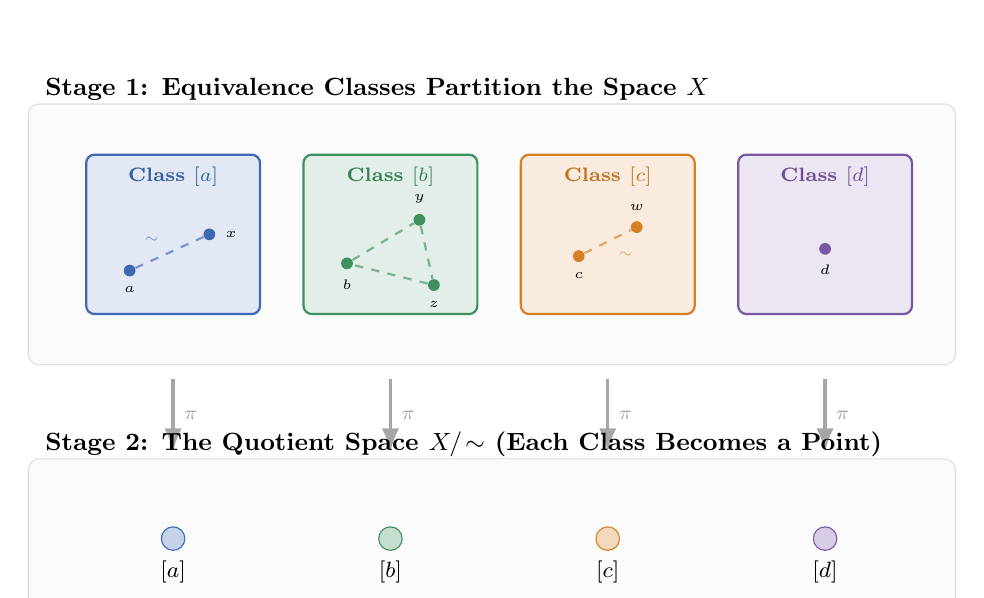
\begin{tikzpicture}[scale=0.92, >=Latex]
  % Stage 1: Partitioned Space X
  \begin{scope}[yshift=0cm]
    \node[anchor=west, font=\small\bfseries] at (-0.5, 3.2) {Stage 1: Equivalence Classes Partition the Space $X$};
    \draw[rounded corners=4pt, fill=gray!3, draw=gray!25] (-0.6, -0.6) rectangle (12.2, 3.0);
    
    % Four cells / tiles
    % Tile 1: [a]
    \draw[thick, sourceblue, fill=sourceblue!15, rounded corners=3pt] (0.2, 0.1) rectangle (2.6, 2.3);
    \node[sourceblue!90!black, font=\scriptsize\bfseries] at (1.4, 2.0) {Class $[a]$};
    \node[circle, fill=sourceblue, inner sep=1.5pt, label={below:\tiny $a$}] (a1) at (0.8, 0.7) {};
    \node[circle, fill=sourceblue, inner sep=1.5pt, label={right:\tiny $x$}] (a2) at (1.9, 1.2) {};
    \draw[thick, sourceblue!70, dashed] (a1) -- node[above left, font=\tiny] {$\sim$} (a2);
    
    % Tile 2: [b]
    \draw[thick, targetgreen, fill=targetgreen!15, rounded corners=3pt] (3.2, 0.1) rectangle (5.6, 2.3);
    \node[targetgreen!90!black, font=\scriptsize\bfseries] at (4.4, 2.0) {Class $[b]$};
    \node[circle, fill=targetgreen, inner sep=1.5pt, label={below:\tiny $b$}] (b1) at (3.8, 0.8) {};
    \node[circle, fill=targetgreen, inner sep=1.5pt, label={above:\tiny $y$}] (b2) at (4.8, 1.4) {};
    \node[circle, fill=targetgreen, inner sep=1.5pt, label={below:\tiny $z$}] (b3) at (5.0, 0.5) {};
    \draw[thick, targetgreen!70, dashed] (b1) -- (b2) -- (b3) -- (b1);
    
    % Tile 3: [c]
    \draw[thick, quotientorange, fill=quotientorange!15, rounded corners=3pt] (6.2, 0.1) rectangle (8.6, 2.3);
    \node[quotientorange!90!black, font=\scriptsize\bfseries] at (7.4, 2.0) {Class $[c]$};
    \node[circle, fill=quotientorange, inner sep=1.5pt, label={below:\tiny $c$}] (c1) at (7.0, 0.9) {};
    \node[circle, fill=quotientorange, inner sep=1.5pt, label={above:\tiny $w$}] (c2) at (7.8, 1.3) {};
    \draw[thick, quotientorange!70, dashed] (c1) -- node[below right, font=\tiny] {$\sim$} (c2);
    
    % Tile 4: [d]
    \draw[thick, structurepurple, fill=structurepurple!15, rounded corners=3pt] (9.2, 0.1) rectangle (11.6, 2.3);
    \node[structurepurple!90!black, font=\scriptsize\bfseries] at (10.4, 2.0) {Class $[d]$};
    \node[circle, fill=structurepurple, inner sep=1.5pt, label={below:\tiny $d$}] (d1) at (10.4, 1.0) {};
  \end{scope}

  % Middle Corridor: Canonical Projection Map
  \begin{scope}[yshift=-1.4cm]
    \draw[->, very thick, gray!70] (1.4, 0.6) -- node[right, font=\scriptsize] {$\pi$} (1.4, -0.4);
    \draw[->, very thick, gray!70] (4.4, 0.6) -- node[right, font=\scriptsize] {$\pi$} (4.4, -0.4);
    \draw[->, very thick, gray!70] (7.4, 0.6) -- node[right, font=\scriptsize] {$\pi$} (7.4, -0.4);
    \draw[->, very thick, gray!70] (10.4, 0.6) -- node[right, font=\scriptsize] {$\pi$} (10.4, -0.4);
  \end{scope}

  % Stage 2: Quotient Space X / ~
  \begin{scope}[yshift=-3.3cm]
    \node[anchor=west, font=\small\bfseries] at (-0.5, 1.6) {Stage 2: The Quotient Space $X/\!\sim$ (Each Class Becomes a Point)};
    \draw[rounded corners=4pt, fill=gray!3, draw=gray!25] (-0.6, -0.7) rectangle (12.2, 1.4);
    
    \node[circle, draw=sourceblue, fill=sourceblue!30, inner sep=3pt, label={below:\footnotesize $[a]$}] at (1.4, 0.3) {};
    \node[circle, draw=targetgreen, fill=targetgreen!30, inner sep=3pt, label={below:\footnotesize $[b]$}] at (4.4, 0.3) {};
    \node[circle, draw=quotientorange, fill=quotientorange!30, inner sep=3pt, label={below:\footnotesize $[c]$}] at (7.4, 0.3) {};
    \node[circle, draw=structurepurple, fill=structurepurple!30, inner sep=3pt, label={below:\footnotesize $[d]$}] at (10.4, 0.3) {};
  \end{scope}
\end{tikzpicture}
\end{center}

\begin{theorem}[Fundamental Theorem of Equivalence Relations]
Let $\sim$ be an equivalence relation on $A$.
\begin{enumerate}[label=(\alph*)]
\item For any $a, b \in A$, $a \sim b \iff [a] = [b]$.
\item Any two equivalence classes are either strictly disjoint or completely identical:
\[
[a] \cap [b] \neq \emptyset \implies [a] = [b].
\]
\item The collection of all equivalence classes forms a \textbf{partition} of $A$: they are pairwise disjoint and their union is all of $A$.
\end{enumerate}
\end{theorem}

\begin{definition}[Quotient Set and Projection]
The collection of all equivalence classes of $A$ under $\sim$ is called the \textbf{quotient set}, denoted $A / \!\sim$:
\[
A / \!\sim \; = \{[a] : a \in A\}.
\]
The function $\pi: A \to A / \!\sim$ given by $\pi(a) = [a]$ is called the \textbf{canonical projection map}.
\end{definition}

In the quotient space, each entire equivalence class has collapsed into a single mathematical point.

\subsection{A Canonical Example: Modular Arithmetic}

Let $n$ be a positive integer. We say two integers $a, b \in \Z$ are \emph{congruent modulo $n$}, written $a \equiv b \pmod n$, if their difference is a multiple of $n$:
\[
a \equiv b \pmod n \iff n \mid (a - b).
\]

\begin{theorem}
Congruence modulo $n$ is an equivalence relation on $\Z$.
\end{theorem}

\begin{proof}
We check all three axioms systematically.

\textbf{1. Reflexivity:} Let $a \in \Z$. Then $a - a = 0 = n \cdot 0$. Because $0$ is an integer, $n \mid (a - a)$, so $a \equiv a \pmod n$.

\textbf{2. Symmetry:} Let $a, b \in \Z$ and assume $a \equiv b \pmod n$. 
By definition, $n \mid (a - b)$, meaning $a - b = n k$ for some integer $k$. 
Multiplying both sides by $-1$:
\[
b - a = -(a - b) = -nk = n(-k).
\]
Since $-k \in \Z$, $n \mid (b - a)$, which proves $b \equiv a \pmod n$.

\textbf{3. Transitivity:} Let $a, b, c \in \Z$, and assume $a \equiv b \pmod n$ and $b \equiv c \pmod n$.
Then $a - b = n j$ and $b - c = n k$ for integers $j, k \in \Z$. 
Adding the two equations:
\[
a - c = (a - b) + (b - c) = n j + n k = n(j + k).
\]
Since $j + k$ is an integer, $n \mid (a - c)$, confirming $a \equiv c \pmod n$.

Since reflexivity, symmetry, and transitivity all hold, congruence modulo $n$ is an equivalence relation.
\end{proof}

The quotient set $\Z / \equiv_n$ is the familiar ring $\Z_n = \{[0], [1], \dots, [n-1]\}$, containing exactly $n$ equivalence classes.

\subsection{Why Mathematicians Care: The Universal Construction}

Equivalence relations and quotient sets are how mathematicians manufacture new mathematical universes from old ones:
\begin{itemize}
\item \textbf{Constructing the Rational Numbers $\Q$:} Start with pairs of integers $(p, q)$ with $q \neq 0$. Declare $(p, q) \sim (r, s) \iff ps = qr$. The quotient set is precisely $\Q$.
\item \textbf{Topology and Manifolds:} Take a flat sheet of paper $[0, 1] \times [0, 1]$ and declare $(0, y) \sim (1, y)$ (glue left edge to right edge) and $(x, 0) \sim (x, 1)$ (glue bottom edge to top edge). The resulting quotient space is a 2-dimensional torus (a donut)!
\item \textbf{Abstract Algebra:} Quotients of groups by normal subgroups $G/N$ and rings by ideals $R/I$ are quotient sets equipped with lawful algebraic operations.
\end{itemize}

\subsection{What Quotients Unlocked, Their Limits, and Where We Go Next}

Equivalence relations and quotient sets unlocked one of the greatest creative engines in modern mathematics:
\begin{itemize}
\item \textbf{Constructing new numbers:} We construct the rational numbers $\Q$ as quotient pairs $(p, q) \sim (r, s) \iff ps = qr$, and the real numbers $\R$ as equivalence classes of Cauchy sequences that differ by a null sequence.
\item \textbf{Topological manifolds:} We build spheres, tori, Klein bottles, and projective spaces by declaring boundary points of flat polygons to be equivalent.
\item \textbf{Algebraic classification:} In abstract algebra (Chapter~21), the First Isomorphism Theorem ($G / \ker\phi \cong \operatorname{im}\phi$) demonstrates that every homomorphism is secretly a quotient projection followed by an isomorphism.
\end{itemize}

Yet equivalence relations possess an inescapable structural boundary: they are strictly \textbf{horizontal}. 

An equivalence relation takes a space and flattens it into peer-to-peer classes where every element inside a class has equal status. It is fundamentally incapable of modeling \textbf{vertical hierarchy}:
\begin{itemize}
\item Which elements contain, dominate, or precede other elements?
\item How do we model dependency graphs, compilers, or task scheduling?
\item How do we describe divisibility chains, where $2 \mid 4$ and $4 \mid 12$, but $12$ does not divide $4$?
\end{itemize}

To model vertical hierarchy, we must break the symmetry of equivalence. If $a$ precedes $b$, we cannot allow $b$ to precede $a$ unless they are the exact same object. In Chapter~16, we introduce \textbf{Orders: Another Kind of Relation}, trading symmetry for antisymmetry to explore posets, chains, and lattices.

\subsection{Exercises}

\begin{enumerate}
\item For each relation on $\R$, determine which of the three properties (reflexive, symmetric, transitive) hold:
\begin{enumerate}[label=(\alph*)]
\item $x \sim y \iff |x - y| \le 1$.
\item $x \sim y \iff x - y \in \Q$.
\item $x \sim y \iff xy > 0$.
\end{enumerate}
\item Let $f: A \to B$ be a function. Define a relation $\sim$ on $A$ by
\[
a_1 \sim a_2 \iff f(a_1) = f(a_2).
\]
Prove that $\sim$ is an equivalence relation. What do its equivalence classes represent geometrically?
\item Let $S$ be a set with 4 elements. How many distinct equivalence relations can be defined on $S$? (Hint: Count the number of partitions of a 4-element set, known as the Bell number $B_4$.)
\end{enumerate}

\newpage

\section{Orders: Another Kind of Relation}
\chapterline

In Chapter~15, we studied equivalence relations. An equivalence relation inspects a universe of objects and gathers them into subsets of equivalent elements: two fractions like $2/4$ and $3/6$ represent the same numerical value; two integers sharing a remainder modulo $12$ land on the exact same hour of a clock face. Equivalence partitions a set into disjoint equivalence classes.

An \textbf{order relation} does something different. Rather than grouping items into classes of equivalent elements, an order introduces hierarchy: it specifies which elements precede, contain, or are smaller than other elements.

On the real line $\R$, every pair of numbers is comparable: given $x$ and $y$, either $x < y$, $x = y$, or $x > y$. But many mathematical structures do not arrange themselves along a single linear chain.

Consider getting dressed in the morning. You must put on socks before shoes, and a shirt before a sweater. But which comes first: your left sock or your shirt? Your watch or your belt? Neither. You can put your watch on before or after your shirt without any conflict. The morning routine has a definite hierarchy---you cannot put on shoes before socks---yet the tasks do not form a single straight line. They branch. 

Branching hierarchies appear throughout mathematics: in set theory, $\{1, 2\}$ contains $\{1\}$, but between $\{1, 2\}$ and $\{2, 3\}$, neither is contained in the other. To capture these branching hierarchies, mathematics uses a \textbf{partial order}.

\begin{historybox}
For centuries, mathematicians treated ordering as identical to the real number line, where any two numbers can be compared. When George Boole (\emph{The Laws of Thought}, 1854) and Charles Sanders Peirce (1870s--1880s) expressed logic and set theory algebraically, they observed that subset inclusion $\subseteq$ and implication $\implies$ act like orders, but with a key difference: two subsets or propositions can be \emph{incomparable}.

In the 1930s, Garrett Birkhoff developed modern order theory in \emph{Lattice Theory}. Birkhoff showed that partially ordered sets and lattices connect Boolean algebra, projective geometry, and functional analysis.

Order theory also revealed challenges in social choice. In 1785, the Marquis de Condorcet showed that individual transitive preferences can produce cyclical majority outcomes ($A > B > C > A$). In 1951, Kenneth Arrow proved in his Impossibility Theorem that no ranked voting system can convert individual preferences into a single collective order while satisfying a small set of fair conditions.
\end{historybox}

\subsection{Partial Orders: The Axiomatic Architecture}

\begin{definition}[Partial Order]
A relation $\preceq$ on a set $A$ is a \textbf{partial order} if it satisfies three structural conditions:
\begin{enumerate}[label=(\roman*)]
\item \textbf{Reflexivity:} For all $a \in A$,
\[
a \preceq a.
\]
(Every element is comparable to itself.)
\item \textbf{Antisymmetry:} For all $a, b \in A$,
\[
(a \preceq b \text{ and } b \preceq a) \implies a = b.
\]
(If two elements precede each other, they are identical.)
\item \textbf{Transitivity:} For all $a, b, c \in A$,
\[
(a \preceq b \text{ and } b \preceq c) \implies a \preceq c.
\]
(Precedence flows reliably along chains.)
\end{enumerate}
A set $A$ equipped with a partial order $\preceq$ is called a \textbf{partially ordered set}, or \textbf{poset} $(A, \preceq)$.
\end{definition}

\begin{intuitionbox}
Pay close attention to \emph{antisymmetry}. In an equivalence relation, symmetry means that if $a \sim b$, then $b \sim a$. In an order relation, two distinct elements cannot precede each other: if $a \preceq b$ and $b \preceq a$, then $a$ and $b$ must be equal. No two distinct elements can each be less than or equal to the other.
\end{intuitionbox}

\begin{marginnotebox}
\textbf{Weak versus Strict Orders:} The symbol $\preceq$ represents a \textbf{weak} partial order (analogous to $\le$ or $\subseteq$), where every element is comparable to itself ($a \preceq a$). In contrast, a \textbf{strict} partial order $\prec$ (analogous to $<$ or $\subset$) is defined by $a \prec b \iff (a \preceq b \text{ and } a \neq b)$. It is irreflexive ($a \not\prec a$) and transitive. Mathematicians use ``partial order'' to mean a weak order unless specified otherwise.
\end{marginnotebox}

\begin{recoverybox}
\textbf{Pause and think:} Is the strict inequality relation $<$ on $\R$ a partial order under our definition? Test the three axioms! Reflexivity fails immediately: $5 < 5$ is false. The relation $<$ is a \emph{strict} order. To be a partial order in our standard sense, reflexivity is mandatory, which is why we work with $\le$.
\end{recoverybox}

\subsection{Partial Versus Total Orders}

\begin{definition}[Comparability and Total Order]
Let $(A, \preceq)$ be a poset. Two elements $x, y \in A$ are \textbf{comparable} if $x \preceq y$ or $y \preceq x$. If neither condition holds, $x$ and $y$ are \textbf{incomparable}, written $x \parallel y$.

A partial order $\preceq$ is a \textbf{total order} (or \textbf{linear order}) if every pair of elements is comparable:
\[
(\forall x, y \in A)(x \preceq y \text{ or } y \preceq x).
\]
\end{definition}

On the real numbers $(\R, \le)$, comparability always holds: given $3$ and $\pi$, we know $3 \le \pi$. The real numbers line up in a single unbroken queue with no branching.

Now consider the power set $\pow(\{1, 2, 3\})$ ordered by subset inclusion $\subseteq$. 
Is $\{1\} \subseteq \{2\}$? No.
Is $\{2\} \subseteq \{1\}$? No.
Neither set contains the other. They are incomparable under inclusion: $\{1\} \parallel \{2\}$. The elements do not line up in a single linear chain; they form a partially ordered set.

Similarly, consider the positive integers $\N = \{1, 2, 3, \dots\}$ ordered by divisibility ($a \mid b$). Is $4 \mid 6$? No. Is $6 \mid 4$? No. Thus $4 \parallel 6$. Divisibility allows incomparable elements that do not divide each other. Divisibility is a genuine partial order, not a total one.

\subsection{Visualizing Posets: Hasse Diagrams}

If we drew every related pair as an arrow in a directed graph, the diagram would quickly become cluttered. For even a small set, reflexive self-loops ($x \preceq x$) appear at every vertex, and transitivity adds many redundant shortcut arrows: if $1 \mid 2$ and $2 \mid 4$, transitivity forces an arrow from $1$ to $4$, from $1$ to $8$, from $1$ to $16$, and so on.

A \textbf{Hasse diagram} (named after the German number theorist Helmut Hasse) strips away this visual noise using three simple rules:
\begin{enumerate}[label=\arabic*.]
\item \textbf{Upward Flow:} If $x \prec y$, place $y$ strictly higher on the page than $x$. Gravity carries the orientation, so arrowheads are unnecessary.
\item \textbf{Omit Reflexive Self-Loops:} Reflexivity ($x \preceq x$) is understood implicitly; no loops are drawn.
\item \textbf{Omit Transitive Shortcuts:} Draw an edge between $x$ and $y$ only if $y$ \emph{covers} $x$.
\end{enumerate}

\begin{definition}[Covering Relation]
Let $(A, \preceq)$ be a poset. We say that $y$ \textbf{covers} $x$ (written $x \lessdot y$) if $x \prec y$ and there is no intermediate element $z \in A$ such that $x \prec z \prec y$.
\end{definition}

In plain words, $y$ covers $x$ if $y$ is an immediate next rung above $x$ on the ladder, with no intervening elements between them. A Hasse diagram draws only the covering edges, letting your eyes reconstruct the full partial order by tracing upward paths.

\begin{figure}[htbp]
\centering
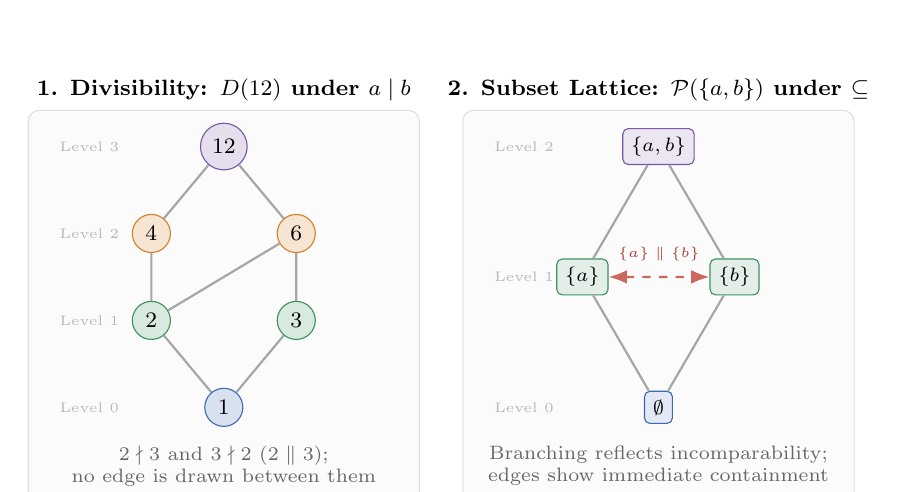
\begin{tikzpicture}[scale=0.92, >=Latex]
  % Panel 1: Divisibility Poset D(12)
  \begin{scope}[xshift=0cm]
    \node[anchor=south, font=\footnotesize\bfseries] at (2.4, 4.3) {1. Divisibility: $D(12)$ under $a \mid b$};
    \draw[rounded corners=4pt, fill=gray!3, draw=gray!25] (-0.3, -1.15) rectangle (5.1, 4.3);
    
    % Level indicators on left
    \node[font=\tiny, text=gray!55, anchor=west] at (0.0, 0.2) {Level 0};
    \node[font=\tiny, text=gray!55, anchor=west] at (0.0, 1.4) {Level 1};
    \node[font=\tiny, text=gray!55, anchor=west] at (0.0, 2.6) {Level 2};
    \node[font=\tiny, text=gray!55, anchor=west] at (0.0, 3.8) {Level 3};
    
    % Nodes
    \node[circle, draw=sourceblue, fill=sourceblue!20, inner sep=2.5pt, font=\footnotesize\bfseries] (n1) at (2.4, 0.2) {$1$};
    \node[circle, draw=targetgreen, fill=targetgreen!20, inner sep=2.5pt, font=\footnotesize\bfseries] (n2) at (1.4, 1.4) {$2$};
    \node[circle, draw=targetgreen, fill=targetgreen!20, inner sep=2.5pt, font=\footnotesize\bfseries] (n3) at (3.4, 1.4) {$3$};
    \node[circle, draw=quotientorange, fill=quotientorange!20, inner sep=2.5pt, font=\footnotesize\bfseries] (n4) at (1.4, 2.6) {$4$};
    \node[circle, draw=quotientorange, fill=quotientorange!20, inner sep=2.5pt, font=\footnotesize\bfseries] (n6) at (3.4, 2.6) {$6$};
    \node[circle, draw=structurepurple, fill=structurepurple!20, inner sep=2.5pt, font=\footnotesize\bfseries] (n12) at (2.4, 3.8) {$12$};
    
    % Covering edges (upward flow)
    \draw[thick, gray!70] (n1) -- (n2);
    \draw[thick, gray!70] (n1) -- (n3);
    \draw[thick, gray!70] (n2) -- (n4);
    \draw[thick, gray!70] (n2) -- (n6);
    \draw[thick, gray!70] (n3) -- (n6);
    \draw[thick, gray!70] (n4) -- (n12);
    \draw[thick, gray!70] (n6) -- (n12);
    
    \node[below, font=\scriptsize, align=center, text=gray!80!black] at (2.4, -0.2) {$2 \nmid 3$ and $3 \nmid 2$ ($2 \parallel 3$);\\no edge is drawn between them};
  \end{scope}

  % Panel 2: Power Set Lattice P({a, b})
  \begin{scope}[xshift=6.0cm]
    \node[anchor=south, font=\footnotesize\bfseries] at (2.4, 4.3) {2. Subset Lattice: $\pow(\{a, b\})$ under $\subseteq$};
    \draw[rounded corners=4pt, fill=gray!3, draw=gray!25] (-0.3, -1.15) rectangle (5.1, 4.3);
    
    % Level indicators on left
    \node[font=\tiny, text=gray!55, anchor=west] at (0.0, 0.2) {Level 0};
    \node[font=\tiny, text=gray!55, anchor=west] at (0.0, 2.0) {Level 1};
    \node[font=\tiny, text=gray!55, anchor=west] at (0.0, 3.8) {Level 2};
    
    % Nodes
    \node[draw=sourceblue, fill=sourceblue!15, rounded corners=2pt, font=\scriptsize\bfseries, inner sep=3pt] (p0) at (2.4, 0.2) {$\emptyset$};
    \node[draw=targetgreen, fill=targetgreen!15, rounded corners=2pt, font=\scriptsize\bfseries, inner sep=3pt] (pa) at (1.35, 2.0) {$\{a\}$};
    \node[draw=targetgreen, fill=targetgreen!15, rounded corners=2pt, font=\scriptsize\bfseries, inner sep=3pt] (pb) at (3.45, 2.0) {$\{b\}$};
    \node[draw=structurepurple, fill=structurepurple!15, rounded corners=2pt, font=\scriptsize\bfseries, inner sep=3pt] (pab) at (2.4, 3.8) {$\{a, b\}$};
    
    % Incomparable indicator
    \draw[<->, thick, trapred!80, dashed] (pa) -- node[above=2pt, font=\tiny, text=trapred!90!black] {$\{a\} \parallel \{b\}$} (pb);
    
    % Edges
    \draw[thick, gray!70] (p0) -- (pa);
    \draw[thick, gray!70] (p0) -- (pb);
    \draw[thick, gray!70] (pa) -- (pab);
    \draw[thick, gray!70] (pb) -- (pab);
    
    \node[below, font=\scriptsize, align=center, text=gray!80!black] at (2.4, -0.2) {Branching reflects incomparability;\\edges show immediate containment};
  \end{scope}
\end{tikzpicture}
\caption{Hasse diagrams reduce visual clutter by omitting reflexive self-loops ($x \preceq x$) and redundant transitive shortcuts. \textbf{Left}: The divisibility poset $D(12)$ under $a \mid b$. Because $2 \nmid 3$ and $3 \nmid 2$, the numbers $2$ and $3$ stand side by side without an edge ($2 \parallel 3$). \textbf{Right}: The power set lattice $\pow(\{a, b\})$ under $\subseteq$. Incomparable singletons $\{a\}$ and $\{b\}$ branch outward and reunite at their join $\{a, b\}$.}
\label{16:fig-hasse-diagrams}
\end{figure}

\subsection{Worked Proof: Divisibility as a Poset}

Let $\N = \{1, 2, 3, \dots\}$ be the positive integers. We define the relation $a \preceq b \iff a \mid b$ ($a$ divides $b$).

\begin{theorem}
Divisibility is a partial order on $\N$.
\end{theorem}

\begin{proof}
We verify the three required conditions:

\textbf{1. Reflexivity:} For any $a \in \N$, $a = a \cdot 1$. Since $1 \in \N$, $a \mid a$, so $a \preceq a$.

\textbf{2. Antisymmetry:} Suppose $a \mid b$ and $b \mid a$.
Then there exist positive integers $k, \ell \in \N$ such that $b = k a$ and $a = \ell b$.
Substituting $b$ into the second equation:
\[
a = \ell (k a) = (\ell k) a.
\]
Since $a > 0$, we divide by $a$ to obtain $\ell k = 1$.
Because $\ell$ and $k$ are positive integers, the only solution to $\ell k = 1$ is $\ell = k = 1$.
Substituting $k = 1$ into $b = k a$ yields $b = a$. Hence antisymmetry holds.

\textbf{3. Transitivity:} Suppose $a \mid b$ and $b \mid c$.
Then $b = j a$ and $c = m b$ for some $j, m \in \N$.
Substituting $b$:
\[
c = m (j a) = (m j) a.
\]
Since $m j$ is a positive integer, $a \mid c$. Hence transitivity holds.

Since all three conditions hold, $(\N, \mid)$ is a poset.
\end{proof}

\begin{trapbox}
Notice why we restricted divisibility to positive integers $\N$ rather than all integers $\Z$! 
On $\Z$, $2 \mid (-2)$ (since $-2 = (-1) \cdot 2$) and $(-2) \mid 2$ (since $2 = (-1) \cdot (-2)$). Yet $2 \neq -2$. Antisymmetry fails on $\Z$ because the equation $\ell k = 1$ has two solutions in $\Z$: $\ell = k = 1$ and $\ell = k = -1$. The presence of invertible units ($\pm 1$) means that mutual divisibility in $\Z$ only guarantees $a = \pm b$ (they are associates), not equality. Mathematical definitions require careful domain awareness.
\end{trapbox}

\subsection{Extremal Elements: Maximal, Minimal, Greatest, and Least}

In everyday language, ``maximal'' and ``maximum'' are often used interchangeably. In order theory, they have distinct mathematical meanings.

\begin{definition}[Extremal Elements]
Let $(A, \preceq)$ be a poset, and let $S \subseteq A$ be a subset.
\begin{enumerate}[label=(\roman*)]
\item An element $M \in S$ is the \textbf{greatest element} (or \textbf{maximum}) of $S$ if for every $x \in S$,
\[
x \preceq M.
\]
(Plain meaning: $M$ is greater than or equal to every element in the set.)
\item An element $m \in S$ is a \textbf{maximal element} of $S$ if for all $x \in S$,
\[
m \preceq x \implies x = m.
\]
(Plain meaning: no element in the set is strictly greater than $m$.)
\item An element $L \in S$ is the \textbf{least element} (or \textbf{minimum}) of $S$ if for every $x \in S$,
\[
L \preceq x.
\]
(Plain meaning: $L$ is less than or equal to every element in the set.)
\item An element $\ell \in S$ is a \textbf{minimal element} of $S$ if for all $x \in S$,
\[
x \preceq \ell \implies x = \ell.
\]
(Plain meaning: no element in the set is strictly less than $\ell$.)
\end{enumerate}
\end{definition}

Notice the logical distinction between these conditions:
\begin{itemize}
\item A \textbf{greatest element} must be comparable to, and greater than or equal to, every element in the set ($x \preceq M$ for all $x$).
\item A \textbf{maximal element} only requires that no element in the set is strictly greater than it ($m \preceq x \implies x = m$).
\end{itemize}

Every greatest element is automatically maximal. In a poset that is not totally ordered, a maximal element need not be comparable to other elements; it only needs to have no element strictly above it.

\begin{theorem}[Uniqueness of Greatest and Least Elements]
If a subset $S$ of a poset has a greatest element, that element is unique. Similarly, if $S$ has a least element, it is unique.
\end{theorem}

\begin{proof}
Suppose $M_1, M_2 \in S$ are both greatest elements of $S$. Since $M_1 \in S$ and $M_2$ is a greatest element, $M_1 \preceq M_2$. Reversing roles, since $M_2 \in S$ and $M_1$ is a greatest element, $M_2 \preceq M_1$. By the antisymmetry of $\preceq$, $M_1 = M_2$. The argument for the least element is identical with inequalities reversed.
\end{proof}

While a poset can have at most \emph{one} greatest element, it can easily have \emph{many} maximal elements!

\begin{example}[Maximal Without Maximum]
Let $S = \pow(\{1, 2, 3\}) \setminus \{\emptyset, \{1, 2, 3\}\}$ be the collection of all non-empty proper subsets of $\{1, 2, 3\}$, ordered by $\subseteq$:
\[
S = \big\{ \{1\}, \, \{2\}, \, \{3\}, \, \{1, 2\}, \, \{1, 3\}, \, \{2, 3\} \big\}.
\]
\begin{itemize}
\item The maximal elements of $S$ are $\{1, 2\}$, $\{1, 3\}$, and $\{2, 3\}$. None of these subsets is contained in any other element of $S$. Yet none of them is a greatest element, because $\{1, 2\} \nsupseteq \{2, 3\}$. The set $S$ has three maximal elements and \emph{no} greatest element.
\item Symmetrically, the minimal elements of $S$ are $\{1\}$, $\{2\}$, and $\{3\}$. None contains any other element of $S$, but none is a least element. The set $S$ has three minimal elements and \emph{no} least element.
\end{itemize}
\end{example}

\begin{figure}[htbp]
\centering
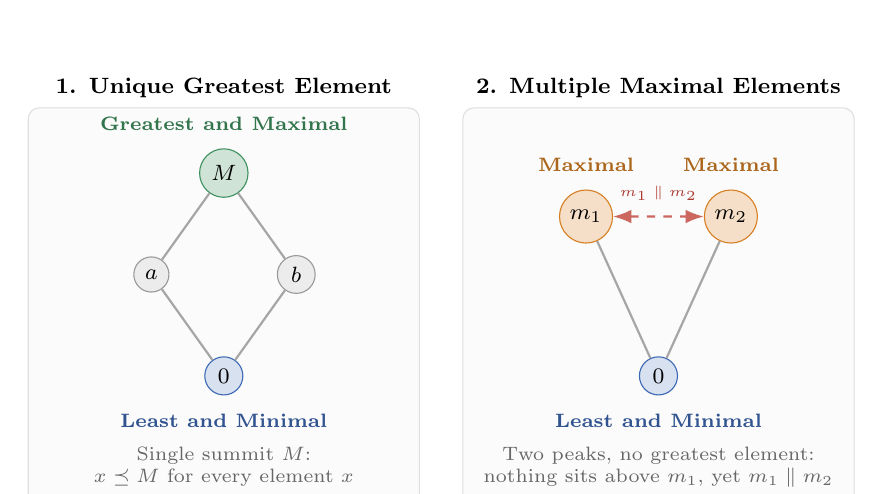
\begin{tikzpicture}[scale=0.92, >=Latex]
  % Panel 1: Unique Greatest Element
  \begin{scope}[xshift=0cm]
    \node[anchor=south, font=\footnotesize\bfseries] at (2.4, 4.3) {1. Unique Greatest Element};
    \draw[rounded corners=4pt, fill=gray!3, draw=gray!25] (-0.3, -1.2) rectangle (5.1, 4.3);
    
    % Nodes
    \node[circle, draw=sourceblue, fill=sourceblue!20, inner sep=2.5pt, font=\footnotesize\bfseries] (b0) at (2.4, 0.6) {$0$};
    \node[circle, draw=gray!80, fill=gray!15, inner sep=2.5pt, font=\footnotesize\bfseries] (ba) at (1.4, 2.0) {$a$};
    \node[circle, draw=gray!80, fill=gray!15, inner sep=2.5pt, font=\footnotesize\bfseries] (bb) at (3.4, 2.0) {$b$};
    \node[circle, draw=targetgreen, fill=targetgreen!25, inner sep=2.5pt, font=\footnotesize\bfseries] (bM) at (2.4, 3.4) {$M$};
    
    % Edges
    \draw[thick, gray!70] (b0) -- (ba);
    \draw[thick, gray!70] (b0) -- (bb);
    \draw[thick, gray!70] (ba) -- (bM);
    \draw[thick, gray!70] (bb) -- (bM);
    
    % Annotations
    \node[above=3pt of bM, font=\scriptsize\bfseries, text=targetgreen!80!black] {Greatest and Maximal};
    \node[below=3pt of b0, font=\scriptsize\bfseries, text=sourceblue!80!black] {Least and Minimal};
    
    \node[below, font=\scriptsize, align=center, text=gray!80!black] at (2.4, -0.25) {Single summit $M$:\\$x \preceq M$ for every element $x$};
  \end{scope}

  % Panel 2: Multiple Maximal Elements
  \begin{scope}[xshift=6.0cm]
    \node[anchor=south, font=\footnotesize\bfseries] at (2.4, 4.3) {2. Multiple Maximal Elements};
    \draw[rounded corners=4pt, fill=gray!3, draw=gray!25] (-0.3, -1.2) rectangle (5.1, 4.3);
    
    % Nodes
    \node[circle, draw=sourceblue, fill=sourceblue!20, inner sep=2.5pt, font=\footnotesize\bfseries] (c0) at (2.4, 0.6) {$0$};
    \node[circle, draw=quotientorange, fill=quotientorange!25, inner sep=2.5pt, font=\footnotesize\bfseries] (cm1) at (1.4, 2.8) {$m_1$};
    \node[circle, draw=quotientorange, fill=quotientorange!25, inner sep=2.5pt, font=\footnotesize\bfseries] (cm2) at (3.4, 2.8) {$m_2$};
    
    % Incomparable indicator at top
    \draw[<->, thick, trapred!80, dashed] (cm1) -- node[above=2pt, font=\tiny, text=trapred!90!black] {$m_1 \parallel m_2$} (cm2);
    
    % Edges
    \draw[thick, gray!70] (c0) -- (cm1);
    \draw[thick, gray!70] (c0) -- (cm2);
    
    % Annotations
    \node[above=3pt of cm1, font=\scriptsize\bfseries, text=quotientorange!80!black] {Maximal};
    \node[above=3pt of cm2, font=\scriptsize\bfseries, text=quotientorange!80!black] {Maximal};
    \node[below=3pt of c0, font=\scriptsize\bfseries, text=sourceblue!80!black] {Least and Minimal};
    
    \node[below, font=\scriptsize, align=center, text=gray!80!black] at (2.4, -0.25) {Two peaks, no greatest element:\\nothing sits above $m_1$, yet $m_1 \parallel m_2$};
  \end{scope}
\end{tikzpicture}
\caption{The vital distinction between a \emph{greatest element} and a \emph{maximal element}. \textbf{Left}: A poset with a single summit $M$. Because $M$ sits above every element ($x \preceq M$ for all $x$), it is the unique greatest element (maximum) and also maximal. \textbf{Right}: A branching poset with two separate peaks $m_1$ and $m_2$. Both $m_1$ and $m_2$ are maximal (no element sits strictly above them), but neither is a greatest element because neither dominates the other ($m_1 \parallel m_2$).}
\label{16:fig-maximal-vs-greatest}
\end{figure}

\begin{recoverybox}
\textbf{Pause and think:} Look at the positive integers with their usual arithmetic order $(\N, \le)$. What is the least element? The number $1$. Is there a maximal element? No: given any $n \in \N$, the number $n+1$ is strictly larger, so no element can be maximal.
\end{recoverybox}

\subsection{Bounds, Suprema, and Lattices}

What happens when a subset of a poset does not contain its own summit, but sits inside a larger universe? We ask what elements in the universe sit above or below it.

\begin{definition}[Bounds, Supremum, and Infimum]
Let $(A, \preceq)$ be a poset, and let $S \subseteq A$.
\begin{enumerate}[label=(\roman*)]
\item An element $u \in A$ is an \textbf{upper bound} for $S$ if $x \preceq u$ for all $x \in S$.
\item If the set of all upper bounds of $S$ has a least element, that element is called the \textbf{least upper bound} or \textbf{supremum} of $S$, written $\sup S$.
\item An element $\ell \in A$ is a \textbf{lower bound} for $S$ if $\ell \preceq x$ for all $x \in S$.
\item If the set of all lower bounds of $S$ has a greatest element, that element is called the \textbf{greatest lower bound} or \textbf{infimum} of $S$, written $\inf S$.
\end{enumerate}
\end{definition}

An upper bound is an element that sits above or at every element of $S$. The supremum is the least among all upper bounds.

When $S$ consists of just two elements $\{a, b\}$, we write:
\[
a \lor b = \sup\{a, b\} \quad (\text{the \textbf{join}}), \qquad a \land b = \inf\{a, b\} \quad (\text{the \textbf{meet}}).
\]
This notation connects familiar operations across different contexts:
\begin{itemize}
\item \textbf{Sets under inclusion ($\subseteq$):} The join is union, and the meet is intersection:
\[
A \lor B = A \cup B, \qquad A \land B = A \cap B.
\]
The union $A \cup B$ is the smallest set that contains both $A$ and $B$; the intersection $A \cap B$ is the largest set contained in both.
\item \textbf{Positive integers under divisibility ($\mid$):} The join is the least common multiple, and the meet is the greatest common divisor:
\[
a \lor b = \operatorname{lcm}(a, b), \qquad a \land b = \gcd(a, b).
\]
The number $\operatorname{lcm}(a, b)$ is the smallest positive integer divisible by both $a$ and $b$; the number $\gcd(a, b)$ is the largest positive integer that divides both.
\item \textbf{Real numbers under standard order ($\le$):} Consider the open interval $S = (0, 1) \subset \R$. Any real number $u \ge 1$ is an upper bound. The lowest upper bound is $\sup S = 1$. Notice that $1 \notin S$: a supremum does not need to belong to the set it bounds! This single observation is central to real analysis (Chapter~20).
\end{itemize}

A poset in which every pair of elements has a meet and a join is called a \textbf{lattice}. In Chapter~31, we will see that lattices provide the algebraic foundation of digital logic circuits, search engines, and set theory.

\begin{center}
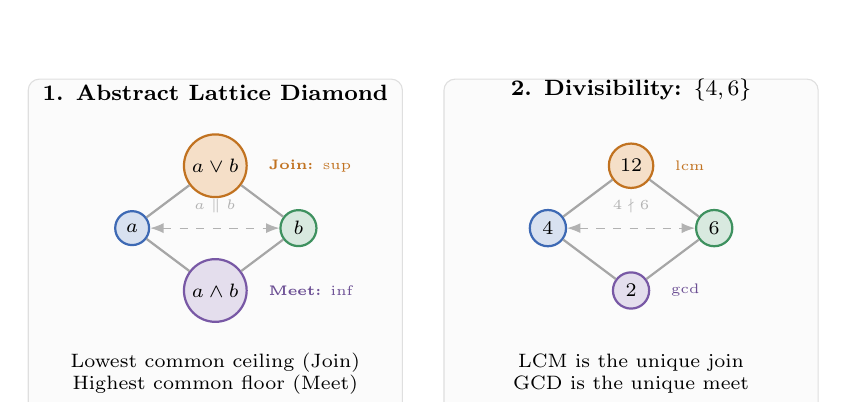
\begin{tikzpicture}[scale=0.88, >=Latex]
  % Panel 1: Abstract Meet and Join
  \begin{scope}[xshift=0cm]
    \draw[rounded corners=4pt, fill=gray!3, draw=gray!25] (-2.7, -2.25) rectangle (2.7, 2.6);
    \node[anchor=south, font=\footnotesize\bfseries] at (0, 2.15) {1. Abstract Lattice Diamond};

    % Top: Join (Supremum)
    \node[circle, draw=quotientorange!90!black, fill=quotientorange!25, thick, inner sep=2pt, font=\scriptsize\bfseries] (sup) at (0, 1.35) {$a \lor b$};
    \node[font=\tiny\bfseries, quotientorange!90!black, right=4pt] at (sup.east) {Join: $\sup$};

    % Middle: a and b
    \node[circle, draw=sourceblue, fill=sourceblue!20, thick, inner sep=2.5pt, font=\scriptsize\bfseries] (na) at (-1.2, 0.45) {$a$};
    \node[circle, draw=targetgreen, fill=targetgreen!20, thick, inner sep=2.5pt, font=\scriptsize\bfseries] (nb) at (1.2, 0.45) {$b$};

    % Incomparable dashed link
    \draw[<->, dashed, gray!60, thin] (na) -- node[above=2pt, font=\tiny, text=gray!60] {$a \parallel b$} (nb);

    % Bottom: Meet (Infimum)
    \node[circle, draw=structurepurple, fill=structurepurple!20, thick, inner sep=2pt, font=\scriptsize\bfseries] (inf) at (0, -0.45) {$a \land b$};
    \node[font=\tiny\bfseries, structurepurple!90!black, right=4pt] at (inf.east) {Meet: $\inf$};

    % Covering edges
    \draw[thick, gray!70] (inf) -- (na);
    \draw[thick, gray!70] (inf) -- (nb);
    \draw[thick, gray!70] (na) -- (sup);
    \draw[thick, gray!70] (nb) -- (sup);

    \node[font=\scriptsize, align=center] at (0, -1.65) {Lowest common ceiling (Join)\\Highest common floor (Meet)};
  \end{scope}

  % Panel 2: Concrete Divisibility Lattice {4, 6}
  \begin{scope}[xshift=6.0cm]
    \draw[rounded corners=4pt, fill=gray!3, draw=gray!25] (-2.7, -2.25) rectangle (2.7, 2.6);
    \node[anchor=south, font=\footnotesize\bfseries] at (0, 2.15) {2. Divisibility: $\{4, 6\}$};

    % Top: LCM = 12
    \node[circle, draw=quotientorange!90!black, fill=quotientorange!25, thick, inner sep=2.5pt, font=\scriptsize\bfseries] (lcm) at (0, 1.35) {$12$};
    \node[font=\tiny\bfseries, quotientorange!90!black, right=4pt] at (lcm.east) {$\operatorname{lcm}$};

    % Middle: 4 and 6
    \node[circle, draw=sourceblue, fill=sourceblue!20, thick, inner sep=2.5pt, font=\scriptsize\bfseries] (d4) at (-1.2, 0.45) {$4$};
    \node[circle, draw=targetgreen, fill=targetgreen!20, thick, inner sep=2.5pt, font=\scriptsize\bfseries] (d6) at (1.2, 0.45) {$6$};

    % Incomparable
    \draw[<->, dashed, gray!60, thin] (d4) -- node[above=2pt, font=\tiny, text=gray!60] {$4 \nmid 6$} (d6);

    % Bottom: GCD = 2
    \node[circle, draw=structurepurple, fill=structurepurple!20, thick, inner sep=2.5pt, font=\scriptsize\bfseries] (gcd) at (0, -0.45) {$2$};
    \node[font=\tiny\bfseries, structurepurple!90!black, right=4pt] at (gcd.east) {$\gcd$};

    % Edges
    \draw[thick, gray!70] (gcd) -- (d4);
    \draw[thick, gray!70] (gcd) -- (d6);
    \draw[thick, gray!70] (d4) -- (lcm);
    \draw[thick, gray!70] (d6) -- (lcm);

    \node[font=\scriptsize, align=center] at (0, -1.65) {LCM is the unique join\\GCD is the unique meet};
  \end{scope}
\end{tikzpicture}\\[0.3em]
{\footnotesize\textbf{Meet, Join, and the Geometry of a Lattice:} \textbf{Left}: For any two elements $a, b$ in a lattice, the join $a \lor b$ is the lowest common ceiling (supremum), and the meet $a \land b$ is the highest common floor (infimum). \textbf{Right}: Under integer divisibility, the join of $4$ and $6$ is their least common multiple $\operatorname{lcm}(4, 6) = 12$, and their meet is their greatest common divisor $\gcd(4, 6) = 2$.}
\end{center}

\subsection{Where Orders Matter and Where We Go Next}

Order theory provides the formal vocabulary for hierarchy across mathematics and computer science:
\begin{itemize}
\item \textbf{Compilers and scheduling:} Task and package dependencies form directed acyclic graphs. Topological sorting extends these partial orders into linear execution pipelines.
\item \textbf{Lattices and digital logic:} Meet and join operations form lattices, which provide the algebraic foundation of Boolean logic and set theory.
\item \textbf{Analysis and bounds:} Concepts like suprema, infima, and completeness in real analysis are defined through posets.
\end{itemize}

An order relation describes how elements line up, but it is a static description. On an infinite ordered set like $\N = \{1, 2, 3, \dots\}$, knowing that $1 < 2 < 3 < \dots$ does not by itself prove a statement for all elements at once.

To prove statements across an infinite sequence of ordered steps, we need an inductive principle. In Chapter~17, we turn to \textbf{Induction: Infinite Claims, Finite Proofs}, which uses the order structure of the natural numbers to establish claims for all $n \in \N$ through finite proofs.

\subsection{Exercises}

\begin{enumerate}
\item \textbf{(Mental Check)} Consider the divisibility poset $(\N, \mid)$ on the positive integers $\N = \{1, 2, 3, \dots\}$.
\begin{enumerate}[label=(\alph*)]
\item Determine whether the following pairs are comparable: $(3, 12)$, $(4, 10)$, and $(7, 7)$.
\item Does $(\N, \mid)$ possess a least element? Does it possess a greatest element?
\item Explain why $(\N, \mid)$ is a partial order but not a total order.
\end{enumerate}

\item \textbf{(Subset Inclusion as a Poset)} Let $S$ be any set. Prove that subset inclusion $\subseteq$ is a partial order on the power set $\pow(S)$ by directly verifying reflexivity, antisymmetry, and transitivity.

\item \textbf{(Hasse Diagram of Divisors)} Draw the Hasse diagram for the divisibility poset on the set of divisors of $30$:
\[
D(30) = \{1, 2, 3, 5, 6, 10, 15, 30\}.
\]
\emph{Hint:} Notice that $30 = 2 \cdot 3 \cdot 5$ is a product of three distinct prime numbers. How does your diagram relate to the three-dimensional cube representing $\pow(\{2, 3, 5\})$?

\item \textbf{(Maximal versus Greatest)} Let $S = \pow(\{1, 2, 3\}) \setminus \{\emptyset, \{1, 2, 3\}\}$ be the collection of all proper, non-empty subsets of $\{1, 2, 3\}$, ordered by subset inclusion $\subseteq$.
\begin{enumerate}[label=(\alph*)]
\item List all maximal elements and all minimal elements of $S$.
\item Does $S$ have a greatest element? Does $S$ have a least element?
\item In your own words, explain how a set can have several maximal elements without having any greatest element.
\end{enumerate}

\item \textbf{(The Product Order)} Let $(A, \preceq_A)$ and $(B, \preceq_B)$ be posets. We define the \emph{product order} $\preceq$ on the Cartesian product $A \times B$ by:
\[
(a_1, b_1) \preceq (a_2, b_2) \iff (a_1 \preceq_A a_2 \text{ and } b_1 \preceq_B b_2).
\]
Prove that $\preceq$ is a partial order on $A \times B$.

\item \textbf{(Lexicographic Order versus Product Order)} Let $(A, \le_A)$ and $(B, \le_B)$ be total orders. The \emph{lexicographic order} (or dictionary order) $\le_{\text{lex}}$ on $A \times B$ is defined by:
\[
(a_1, b_1) \le_{\text{lex}} (a_2, b_2) \iff (a_1 <_A a_2) \text{ or } (a_1 = a_2 \text{ and } b_1 \le_B b_2).
\]
\begin{enumerate}[label=(\alph*)]
\item Prove that if $\le_A$ and $\le_B$ are total orders, then $\le_{\text{lex}}$ is a total order on $A \times B$.
\item Find two points in $\R \times \R$ that are comparable under lexicographic order but incomparable under the product order of Exercise~5.
\end{enumerate}

\item \textbf{(Lattice Operations in Divisibility)} In the divisibility poset $(\N, \mid)$, let $a, b \in \N$.
\begin{enumerate}[label=(\alph*)]
\item Prove that the greatest lower bound $\inf\{a, b\}$ is the greatest common divisor $\gcd(a, b)$.
\item Prove that the least upper bound $\sup\{a, b\}$ is the least common multiple $\operatorname{lcm}(a, b)$.
\end{enumerate}
\end{enumerate}

\newpage

\section{Induction: Infinite Claims, Finite Proofs}
\chapterline

Imagine standing before an infinite line of dominoes stretching past the horizon:
\[
D_1, \; D_2, \; D_3, \; D_4, \; \dots, \; D_n, \; \dots
\]
You wish to ensure that every single domino will eventually topple. 

You could walk down the line and knock each domino over by hand. But because the line is infinite, you would never finish. No matter how many millions of dominoes you tip over, an endless expanse remains untouched.

Instead, you inspect the mechanics of the line and notice two local facts:
\begin{enumerate}[label=\arabic*.]
\item \textbf{The Initial Push:} You physically tip over the very first domino, $D_1$.
\item \textbf{The Chain Reaction:} The dominoes are spaced closely enough that whenever any arbitrary domino $D_k$ falls, its momentum is guaranteed to strike and topple the next domino, $D_{k+1}$.
\end{enumerate}

With those two guarantees in place, every domino in the infinite chain falls: domino $1$ topples $2$, domino $2$ topples $3$, and the pattern continues for every positive integer.

This is the principle of \textbf{mathematical induction}. It is our primary tool for proving an infinite family of statements using a finite chain of deductions.

\begin{historybox}
The formalization of mathematical induction was achieved by Blaise Pascal in his 1654 \emph{Trait\'e du triangle arithm\'etique}. Pascal was collaborating with Pierre de Fermat on the ``problem of points''---how to fairly divide the stakes in an unfinished game of chance. To calculate probabilities, Pascal needed rigorous formulas for binomial coefficients across all rows of his triangle, but he had no way to verify an infinite table one row at a time. He formulated the principle of induction: verify the first row, prove that each row forces the truth of the next, and the entire table is established.

Traces of inductive reasoning had appeared earlier in the work of the 14th-century mathematician Levi ben Gershon (Gersonides) and the Sicilian mathematician Francesco Maurolico (1575), who proved that the sum of the first $n$ odd integers equals $n^2$. But Pascal made the principle explicit and general. 

Two centuries later, Giuseppe Peano (\emph{Arithmetices principia}, 1889) recognized that induction is not just a proof technique; it is the fifth Peano axiom defining what the natural numbers $\N$ are. The natural numbers are precisely the set generated from $1$ by repeatedly applying the successor operation. Induction works because there are no natural numbers outside the sequence generated by repeated succession.
\end{historybox}

\begin{center}
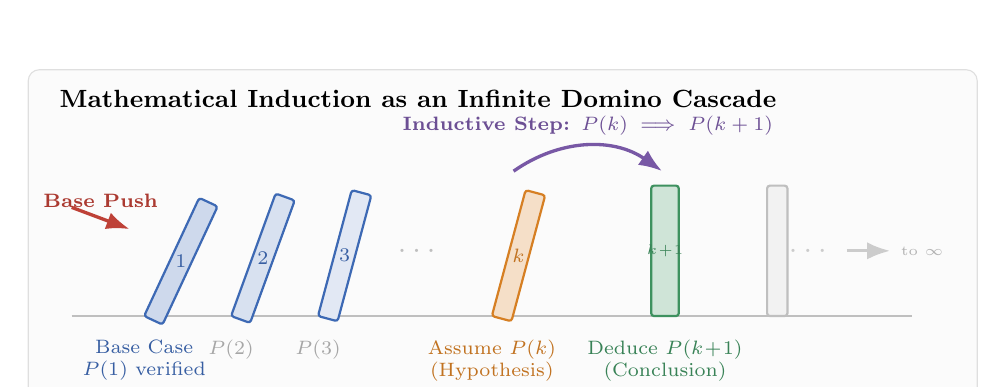
\begin{tikzpicture}[scale=0.92, >=Latex]
  % Stage box
  \draw[rounded corners=4pt, fill=gray!3, draw=gray!25] (-0.6, -1.15) rectangle (12.5, 3.4);
  \node[anchor=west, font=\small\bfseries] at (-0.3, 3.0) {Mathematical Induction as an Infinite Domino Cascade};
  
  % Ground line
  \draw[thick, gray!50] (0.0, 0.0) -- (11.6, 0.0);
  
  % Domino 1: Tipping over (Base case)
  \begin{scope}[shift={(1.0, 0.0)}, rotate around={-25:(0,0)}]
    \draw[thick, sourceblue, fill=sourceblue!25, rounded corners=1pt] (0, 0) rectangle (0.28, 1.8);
    \node[sourceblue!90!black, font=\scriptsize\bfseries] at (0.14, 0.9) {$1$};
  \end{scope}
  \draw[->, very thick, trapred] (0.0, 1.5) -- node[above, font=\scriptsize\bfseries, text=trapred!90!black] {Base Push} (0.8, 1.2);
  \node[below, font=\scriptsize, align=center, text=sourceblue!90!black] at (1.0, -0.2) {Base Case\\$P(1)$ verified};

  % Domino 2: Tipping
  \begin{scope}[shift={(2.2, 0.0)}, rotate around={-20:(0,0)}]
    \draw[thick, sourceblue, fill=sourceblue!20, rounded corners=1pt] (0, 0) rectangle (0.28, 1.8);
    \node[sourceblue!90!black, font=\scriptsize\bfseries] at (0.14, 0.9) {$2$};
  \end{scope}
  \node[below, font=\scriptsize, text=gray!70] at (2.2, -0.2) {$P(2)$};

  % Domino 3: Tipping
  \begin{scope}[shift={(3.4, 0.0)}, rotate around={-15:(0,0)}]
    \draw[thick, sourceblue, fill=sourceblue!15, rounded corners=1pt] (0, 0) rectangle (0.28, 1.8);
    \node[sourceblue!90!black, font=\scriptsize\bfseries] at (0.14, 0.9) {$3$};
  \end{scope}
  \node[below, font=\scriptsize, text=gray!70] at (3.4, -0.2) {$P(3)$};

  % Dots
  \node[font=\large\bfseries, text=gray!50] at (4.8, 0.9) {$\dots$};

  % Domino k (Hypothesis)
  \begin{scope}[shift={(5.8, 0.0)}, rotate around={-15:(0,0)}]
    \draw[thick, quotientorange, fill=quotientorange!25, rounded corners=1pt] (0, 0) rectangle (0.28, 1.8);
    \node[quotientorange!90!black, font=\scriptsize\bfseries] at (0.14, 0.9) {$k$};
  \end{scope}
  \node[below, font=\scriptsize, align=center, text=quotientorange!90!black] at (5.8, -0.2) {Assume $P(k)$\\(Hypothesis)};

  % Domino k+1 (Target)
  \begin{scope}[shift={(8.0, 0.0)}]
    \draw[thick, targetgreen, fill=targetgreen!25, rounded corners=1pt] (0, 0) rectangle (0.38, 1.8);
    \node[targetgreen!90!black, font=\tiny\bfseries] at (0.19, 0.9) {$k\!+\!1$};
  \end{scope}
  \node[below, font=\scriptsize, align=center, text=targetgreen!90!black] at (8.19, -0.2) {Deduce $P(k\!+\!1)$\\(Conclusion)};

  % Inductive Bridge Arc
  \draw[->, very thick, structurepurple] (6.1, 2.0) to[bend left=35] node[above, font=\scriptsize\bfseries, text=structurepurple!90!black] {Inductive Step: $P(k) \implies P(k+1)$} (8.15, 2.0);

  % Domino k+2 and beyond
  \begin{scope}[shift={(9.6, 0.0)}]
    \draw[thick, gray!50, fill=gray!10, rounded corners=1pt] (0, 0) rectangle (0.28, 1.8);
  \end{scope}
  \node[font=\large\bfseries, text=gray!40] at (10.2, 0.9) {$\dots$};
  \draw[->, very thick, gray!40] (10.7, 0.9) -- (11.3, 0.9) node[right, font=\tiny, text=gray!60] {to $\infty$};
\end{tikzpicture}\\[0.4em]
{\small\textbf{Figure 17.1:} Mathematical induction as an infinite cascade. An initial manual push establishes the base case $P(1)$. The conditional guarantee $P(k) \implies P(k+1)$ acts like the close spacing between dominoes: whenever any domino $k$ falls, it knocks over $k+1$. Together, these two finite proofs guarantee that every domino in the infinite sequence falls.}
\end{center}

\subsection{The Formal Principle of Mathematical Induction}

To make the domino intuition mathematically rigorous, we replace dominoes with mathematical statements.

Recall from Chapter~2 that a \textbf{predicate} is an open statement containing a variable slot, such as $P(n): \text{``}2^n \ge n+1\text{''}$. By itself, a predicate is neither true nor false; it converts into a definite assertion with a truth value only when a specific number is plugged into the slot.

\begin{theorem}[Principle of Mathematical Induction]
Let $P(n)$ be a predicate parameterized by integers $n \ge n_0$. Suppose that:
\begin{enumerate}[label=(\roman*)]
\item \textbf{Base Case:} $P(n_0)$ is true.
\item \textbf{Inductive Step:} For every integer $k \ge n_0$, if $P(k)$ is true, then $P(k+1)$ is true:
\[
(\forall k \ge n_0)(P(k) \implies P(k+1)).
\]
\end{enumerate}
Then $P(n)$ is true for all integers $n \ge n_0$.
\end{theorem}

\begin{walkbox}
\textbf{Mental Check:} Suppose you verify the base case at $n_0 = 4$, and you prove that $P(k) \implies P(k+1)$ for all $k \ge 4$. Does this theorem guarantee that $P(2)$ is true?
\emph{Answer:} No. The domino cascade only travels forward from the base case. Dominoes prior to the starting push ($n < n_0$) remain untouched and unverified.
\end{walkbox}

\begin{intuitionbox}
A common question when first learning induction is: ``In the inductive step, aren't we assuming what we set out to prove?''

No: you are not asserting that $P(n)$ is universally true. You are proving an implication: if $P(k)$ holds, then $P(k+1)$ holds.

In the inductive step, you assume $P(k)$ hypothetically for an arbitrary $k \ge n_0$, and use that assumption to deduce $P(k+1)$. You are proving the validity of the conditional statement $P(k) \implies P(k+1)$. The base case then establishes the starting truth $P(n_0)$, allowing the truth of the statement to propagate to all subsequent integers.
\end{intuitionbox}

\subsection{A Worked Example: Gauss's Triangular Sum}

Consider the classical formula for the sum of the first $n$ positive integers:
\[
1 + 2 + 3 + \dots + n = \frac{n(n+1)}{2}.
\]
Before writing down any algebra, pause to see the visual geometry. If you arrange dots in a triangular staircase of height $n$, you can fit two such staircases together to form an $n \times (n+1)$ rectangle containing $n(n+1)$ dots. Half of that rectangle gives the total count (Figure~17.2).

\begin{center}
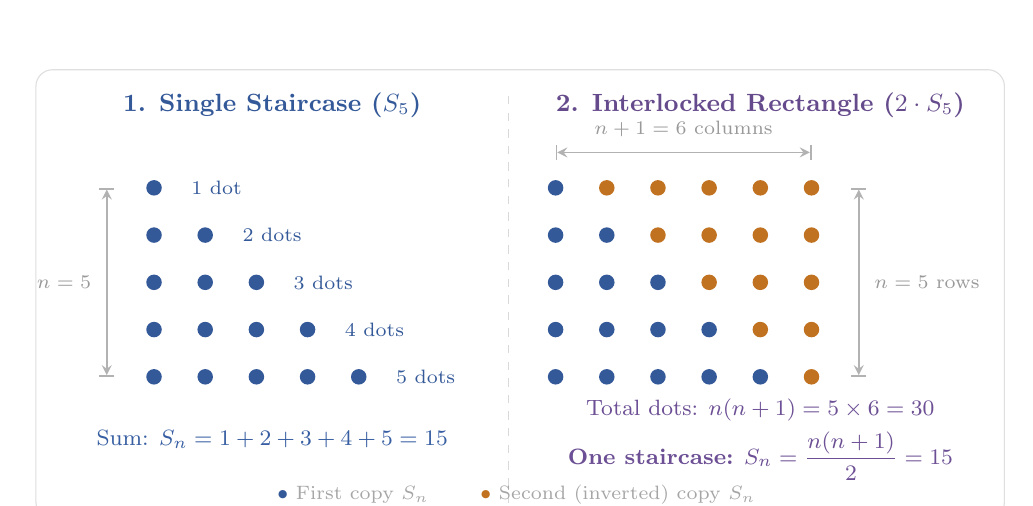
\begin{tikzpicture}[>=stealth, font=\small]
  % Card background container
  \draw[fill=white, draw=gray!25, rounded corners=6pt] (-0.8, -0.9) rectangle (11.5, 4.8);
  \draw[dashed, gray!30] (5.2, -0.7) -- (5.2, 4.5);

  % Panel 1: Single Staircase
  \node[font=\small\bfseries, sourceblue!85!black] at (2.2, 4.35) {1. Single Staircase ($S_5$)};

  % Panel 1 Dots (Blue)
  \foreach \c in {1} { \fill[sourceblue!85!black] ({0.7 + (\c-1)*0.65}, 3.3) circle (2.8pt); }
  \foreach \c in {1,2} { \fill[sourceblue!85!black] ({0.7 + (\c-1)*0.65}, 2.7) circle (2.8pt); }
  \foreach \c in {1,2,3} { \fill[sourceblue!85!black] ({0.7 + (\c-1)*0.65}, 2.1) circle (2.8pt); }
  \foreach \c in {1,2,3,4} { \fill[sourceblue!85!black] ({0.7 + (\c-1)*0.65}, 1.5) circle (2.8pt); }
  \foreach \c in {1,2,3,4,5} { \fill[sourceblue!85!black] ({0.7 + (\c-1)*0.65}, 0.9) circle (2.8pt); }

  % Panel 1 Row counts
  \node[right, font=\scriptsize, text=sourceblue!85!black] at (1.05, 3.3) {$1$ dot};
  \node[right, font=\scriptsize, text=sourceblue!85!black] at (1.70, 2.7) {$2$ dots};
  \node[right, font=\scriptsize, text=sourceblue!85!black] at (2.35, 2.1) {$3$ dots};
  \node[right, font=\scriptsize, text=sourceblue!85!black] at (3.00, 1.5) {$4$ dots};
  \node[right, font=\scriptsize, text=sourceblue!85!black] at (3.65, 0.9) {$5$ dots};

  % Panel 1 Dimension bar
  \draw[|<->|, >=stealth, gray!60, semithick] (0.1, 0.9) -- (0.1, 3.3) node[midway, left=2pt, font=\scriptsize, text=gray!80] {$n = 5$};

  % Panel 1 Summary
  \node[font=\footnotesize, align=center, text=sourceblue!90!black] at (2.2, 0.1) {Sum: $S_n = 1 + 2 + 3 + 4 + 5 = 15$};

  % Panel 2: Interlocked Rectangle
  \node[font=\small\bfseries, structurepurple!85!black] at (8.4, 4.35) {2. Interlocked Rectangle ($2 \cdot S_5$)};

  % Panel 2 Blue Dots (First Staircase)
  \foreach \c in {1} { \fill[sourceblue!85!black] ({5.8 + (\c-1)*0.65}, 3.3) circle (2.8pt); }
  \foreach \c in {1,2} { \fill[sourceblue!85!black] ({5.8 + (\c-1)*0.65}, 2.7) circle (2.8pt); }
  \foreach \c in {1,2,3} { \fill[sourceblue!85!black] ({5.8 + (\c-1)*0.65}, 2.1) circle (2.8pt); }
  \foreach \c in {1,2,3,4} { \fill[sourceblue!85!black] ({5.8 + (\c-1)*0.65}, 1.5) circle (2.8pt); }
  \foreach \c in {1,2,3,4,5} { \fill[sourceblue!85!black] ({5.8 + (\c-1)*0.65}, 0.9) circle (2.8pt); }

  % Panel 2 Orange Dots (Inverted Second Staircase)
  \foreach \c in {2,3,4,5,6} { \fill[quotientorange!90!black] ({5.8 + (\c-1)*0.65}, 3.3) circle (2.8pt); }
  \foreach \c in {3,4,5,6} { \fill[quotientorange!90!black] ({5.8 + (\c-1)*0.65}, 2.7) circle (2.8pt); }
  \foreach \c in {4,5,6} { \fill[quotientorange!90!black] ({5.8 + (\c-1)*0.65}, 2.1) circle (2.8pt); }
  \foreach \c in {5,6} { \fill[quotientorange!90!black] ({5.8 + (\c-1)*0.65}, 1.5) circle (2.8pt); }
  \foreach \c in {6} { \fill[quotientorange!90!black] ({5.8 + (\c-1)*0.65}, 0.9) circle (2.8pt); }

  % Panel 2 Dimension bars
  \draw[|<->|, >=stealth, gray!60, semithick] (5.8, 3.75) -- (9.05, 3.75) node[midway, above=2pt, font=\scriptsize, text=gray!80] {$n + 1 = 6$ columns};
  \draw[|<->|, >=stealth, gray!60, semithick] (9.65, 0.9) -- (9.65, 3.3) node[midway, right=2pt, font=\scriptsize, text=gray!80] {$n = 5$ rows};

  % Panel 2 Summary
  \node[font=\footnotesize, align=center, text=structurepurple!90!black] at (8.4, 0.1) {Total dots: $n(n+1) = 5 \times 6 = 30$\\[3pt]\textbf{One staircase:} $S_n = \dfrac{n(n+1)}{2} = 15$};

  % Legend below
  \node[font=\scriptsize, text=gray!70] at (5.3, -0.6) {{\color{sourceblue!85!black}$\bullet$} First copy $S_n$ \qquad {\color{quotientorange!90!black}$\bullet$} Second (inverted) copy $S_n$};
\end{tikzpicture}\\[0.4em]
{\small\textbf{Figure 17.2:} Visual proof of Gauss's triangular sum $\sum_{i=1}^n i = \frac{n(n+1)}{2}$. \emph{Left:} Dots arranged in a triangular staircase of height $n=5$, where row $i$ contains $i$ dots. \emph{Right:} Two congruent copies of the staircase (blue and orange) interlock to form an $n \times (n+1)$ rectangular grid. The rectangle contains $n(n+1)$ dots, so each staircase contains exactly half: $\frac{n(n+1)}{2}$.}
\end{center}

Now let us prove this identity rigorously for every integer $n \ge 1$ using mathematical induction.

\begin{theorem}
For all integers $n \ge 1$,
\[
\sum_{i=1}^n i = \frac{n(n+1)}{2}.
\]
\end{theorem}

\begin{proof}
Let $P(n)$ be the statement that $\sum_{i=1}^n i = \frac{n(n+1)}{2}$.

\textbf{Base Case ($n = 1$):}
For $n = 1$, the left-hand side is the single term $1$.
The right-hand side is
\[
\frac{1(1 + 1)}{2} = \frac{1(2)}{2} = 1.
\]
Both sides evaluate to $1$, so the base case $P(1)$ is verified.

\textbf{Inductive Step:}
Let $k \ge 1$ be an arbitrary integer. Assume that $P(k)$ is true, meaning
\[
1 + 2 + \dots + k = \frac{k(k+1)}{2}. \tag{Induction Hypothesis}
\]
We must prove that $P(k+1)$ holds, which means establishing:
\[
1 + 2 + \dots + k + (k+1) = \frac{(k+1)((k+1)+1)}{2} = \frac{(k+1)(k+2)}{2}.
\]

We begin with the sum of the first $k+1$ terms and isolate the sum of the first $k$ terms:
\[
\underbrace{1 + 2 + \dots + k}_{= \frac{k(k+1)}{2} \text{ by hypothesis}} + (k+1).
\]
Substituting our induction hypothesis:
\[
1 + 2 + \dots + k + (k+1) = \frac{k(k+1)}{2} + (k+1).
\]
Rather than expanding everything into quadratic polynomials, we notice the common factor of $(k+1)$ and factor it out cleanly:
\begin{align*}
\frac{k(k+1)}{2} + (k+1) 
&= (k+1)\left(\frac{k}{2} + 1\right) \\
&= (k+1)\left(\frac{k+2}{2}\right) \\
&= \frac{(k+1)(k+2)}{2}.
\end{align*}
This is precisely the formula demanded by $P(k+1)$.

Having verified the base case and established that $P(k) \implies P(k+1)$ for all $k \ge 1$, the Principle of Mathematical Induction implies that the formula holds for all integers $n \ge 1$.
\end{proof}

\begin{walkbox}
\textbf{Mental Check:} In the inductive step above, why did we peel off the last term $(k+1)$ before doing any algebra?
\emph{Answer:} Because our sole point of leverage is the induction hypothesis, which only speaks about sums of length $k$. Isolating the first $k$ terms creates the exact slot where our hypothesis can be legally applied.
\end{walkbox}

\subsection{Induction With Inequalities}

Induction is not limited to algebraic equalities; it frequently establishes growth rates and bounds in analysis.

When proving an equality by induction, both sides must match exactly. With inequalities, the induction step often yields a quantity strictly larger than needed. The goal is to bound terms in the correct direction rather than maintaining equality.

\begin{theorem}
For all integers $n \ge 1$, $2^n \ge n + 1$.
\end{theorem}

\begin{proof}
Let $P(n)$ be the inequality $2^n \ge n + 1$.

\textbf{Base Case ($n = 1$):} For $n = 1$, the left side is $2^1 = 2$ and the right side is $1 + 1 = 2$. Since $2 \ge 2$, the base case $P(1)$ holds.

\textbf{Inductive Step:} Let $k \ge 1$ be an arbitrary integer. Assume that $P(k)$ is true:
\[
2^k \ge k + 1. \tag{Induction Hypothesis}
\]
We must prove $P(k+1)$: that $2^{k+1} \ge (k+1) + 1 = k + 2$.

We start with the left side of our target inequality, expressing $2^{k+1}$ in terms of $2^k$:
\[
2^{k+1} = 2 \cdot 2^k.
\]
Because $2 > 0$, multiplying both sides of our induction hypothesis by $2$ preserves the inequality:
\[
2^{k+1} = 2 \cdot 2^k \ge 2(k + 1) = 2k + 2.
\]
Now we split $2k + 2$ to reveal our desired target $k + 2$:
\[
2k + 2 = k + k + 2.
\]
Because $k \ge 1$, the extra term $k$ is at least $1$. Therefore:
\[
2^{k+1} \ge k + k + 2 \ge 1 + k + 2 = k + 3 > k + 2.
\]
Since $2^{k+1} > k + 2$, it certainly follows that $2^{k+1} \ge k + 2$. This completes the inductive step.

By the Principle of Mathematical Induction, $2^n \ge n + 1$ for all integers $n \ge 1$.
\end{proof}

\subsection{Induction on Divisibility Statements}

A third common application of induction is divisibility in number theory.

Recall the definition from Chapter~6: for integers $a$ and $b$, we say $a \mid b$ ($a$ divides $b$) if there exists an integer $m$ such that $b = a \cdot m$.

When proving by induction that an algebraic expression is divisible by $d$, a systematic strategy is:
\begin{enumerate}[label=\arabic*.]
\item \textbf{State the Hypothesis:} Write the $k$-th expression as $d \cdot m$ for some integer $m$.
\item \textbf{Expand the Target:} Write out the $(k+1)$-th expression.
\item \textbf{Isolate the Hypothesis:} Regroup the expanded terms to separate out the $k$-th expression.
\item \textbf{Substitute and Factor:} Replace the $k$-th expression with $d \cdot m$, and factor $d$ out of the remaining terms.
\end{enumerate}

\begin{theorem}
For all integers $n \ge 1$, $3$ divides $n^3 + 2n$.
\end{theorem}

\begin{proof}
Let $P(n)$ be the predicate that $3 \mid (n^3 + 2n)$.

\textbf{Base Case ($n = 1$):}
For $n = 1$, the expression evaluates to:
\[
1^3 + 2(1) = 1 + 2 = 3 = 3 \cdot 1.
\]
Because $3$ is an integer multiple of $3$, the base case $P(1)$ is verified.

\textbf{Inductive Step:}
Let $k \ge 1$ be an arbitrary integer. Assume $P(k)$ is true: there exists an integer $m$ such that
\[
k^3 + 2k = 3m. \tag{Induction Hypothesis}
\]
We must prove $P(k+1)$: that $(k+1)^3 + 2(k+1)$ is an integer multiple of $3$.

We expand $(k+1)^3 + 2(k+1)$:
\begin{align*}
(k+1)^3 + 2(k+1) 
&= (k^3 + 3k^2 + 3k + 1) + (2k + 2) \\
&= k^3 + 3k^2 + 5k + 3.
\end{align*}
We isolate the expression from our induction hypothesis, $k^3 + 2k$. Grouping $k^3$ together with $2k$ leaves the remaining terms together:
\[
(k+1)^3 + 2(k+1) = (k^3 + 2k) + (3k^2 + 3k + 3).
\]
By our induction hypothesis, $k^3 + 2k = 3m$. Substituting this into our expression:
\begin{align*}
(k+1)^3 + 2(k+1) 
&= 3m + 3(k^2 + k + 1) \\
&= 3\bigl(m + k^2 + k + 1\bigr).
\end{align*}
Because $m$ and $k$ are integers, $q = m + k^2 + k + 1$ is an integer. Thus $(k+1)^3 + 2(k+1) = 3q$, proving that $3 \mid ((k+1)^3 + 2(k+1))$.

By the Principle of Mathematical Induction, $3 \mid (n^3 + 2n)$ for all integers $n \ge 1$.
\end{proof}

\begin{trapbox}
\textbf{Common Mistakes in Induction Proofs:}
\begin{enumerate}
\item \emph{Omitting or mishandling the base case:} Without a verified base case, an inductive implication proves nothing. For instance, the implication $n = n + 1 \implies n+1 = (n+1) + 1$ is a valid logical conditional, but $n = n+1$ is false for every integer because no base case holds to begin the chain.
\item \emph{Assuming the target $P(k+1)$:} You must adopt the predecessor case $P(k)$ as your working hypothesis and deduce $P(k+1)$. Assuming $P(k+1)$ at the outset is circular logic.
\item \emph{Proving the inductive step for only a specific number:} Proving $P(1) \implies P(2)$ and $P(2) \implies P(3)$ does not prove the theorem. The inductive step must be established for an \emph{arbitrary} integer $k \ge n_0$.
\item \emph{Hiding or ignoring the induction hypothesis:} If your proof of $P(k+1)$ never uses $P(k)$, you are either performing direct algebra (which did not need induction in the first place) or your deduction contains a hidden hole. Always explicitly flag where the induction hypothesis is invoked.
\end{enumerate}

\textbf{P\'olya's Horse Fallacy: The Hidden Disconnect}

To see how a subtle defect in the inductive step can prove absurdities, consider George P\'olya's famous paradox: ``Prove that all horses have the same color.''
\begin{itemize}
\item \emph{Base Case ($n=1$):} In any set consisting of a single horse, every horse trivially shares the same color, because there is only one horse.
\item \emph{Inductive Step:} Assume that in any set of $k$ horses, all horses have the identical color. Now consider any set of $k+1$ horses, numbered $\{h_1, h_2, \dots, h_{k+1}\}$. 
Remove horse $h_{k+1}$; the remaining $k$ horses $\{h_1, h_2, \dots, h_k\}$ have the same color by our induction hypothesis. 
Now replace $h_{k+1}$ and remove $h_1$; the remaining $k$ horses $\{h_2, \dots, h_{k+1}\}$ also have the same color. 
Because both groups overlap, all $k+1$ horses must have the same color!
\end{itemize}

Where does this deduction collapse? Look at the transition from $k=1$ to $k+1=2$ illustrated in Figure~17.3!
\end{trapbox}

\begin{center}
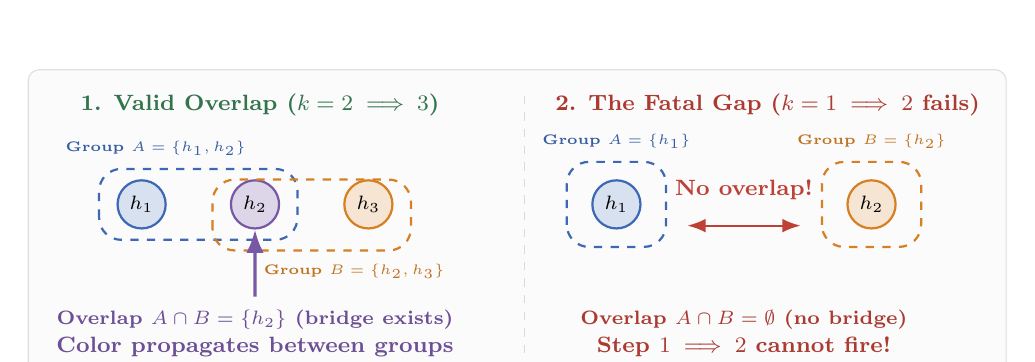
\begin{tikzpicture}[scale=0.9, >=Latex]
  % Stage box
  \draw[rounded corners=4pt, fill=gray!3, draw=gray!25] (-0.5, -0.9) rectangle (13.3, 3.4);

  % Panel 1: k=2 (3 horses) -> Overlap works
  \begin{scope}[xshift=0.3cm, yshift=0.1cm]
    \node[anchor=west, font=\footnotesize\bfseries, text=targetgreen!80!black] at (-0.2, 2.8) {1. Valid Overlap ($k=2 \implies 3$)};

    % Horse nodes
    \node[circle, draw=sourceblue, fill=sourceblue!20, thick, inner sep=2.5pt, font=\scriptsize\bfseries] (h1) at (0.8, 1.4) {$h_1$};
    \node[circle, draw=structurepurple, fill=structurepurple!25, thick, inner sep=2.5pt, font=\scriptsize\bfseries] (h2) at (2.4, 1.4) {$h_2$};
    \node[circle, draw=quotientorange, fill=quotientorange!20, thick, inner sep=2.5pt, font=\scriptsize\bfseries] (h3) at (4.0, 1.4) {$h_3$};

    % Group A oval enclosing h1, h2
    \draw[thick, sourceblue, dashed, rounded corners=8pt] (0.2, 0.9) rectangle (3.0, 1.9);
    \node[sourceblue!90!black, font=\tiny\bfseries, anchor=south] at (1.0, 1.95) {Group $A = \{h_1, h_2\}$};

    % Group B oval enclosing h2, h3
    \draw[thick, quotientorange, dashed, rounded corners=8pt] (1.8, 0.75) rectangle (4.6, 1.75);
    \node[quotientorange!90!black, font=\tiny\bfseries, anchor=north] at (3.8, 0.7) {Group $B = \{h_2, h_3\}$};

    % Overlap annotation
    \draw[->, very thick, structurepurple] (2.4, 0.1) -- (h2);
    \node[below, font=\scriptsize\bfseries, text=structurepurple!90!black, align=center] at (2.4, 0.05) {Overlap $A \cap B = \{h_2\}$ (bridge exists)\\[2pt]\footnotesize Color propagates between groups};
  \end{scope}

  % Divider
  \draw[dashed, gray!30] (6.5, -0.6) -- (6.5, 3.1);

  % Panel 2: k=1 (2 horses) -> Overlap collapses!
  \begin{scope}[xshift=7.0cm, yshift=0.1cm]
    \node[anchor=west, font=\footnotesize\bfseries, text=trapred!90!black] at (-0.2, 2.8) {2. The Fatal Gap ($k=1 \implies 2$ fails)};

    % Horse nodes
    \node[circle, draw=sourceblue, fill=sourceblue!20, thick, inner sep=2.5pt, font=\scriptsize\bfseries] (x1) at (0.8, 1.4) {$h_1$};
    \node[circle, draw=quotientorange, fill=quotientorange!20, thick, inner sep=2.5pt, font=\scriptsize\bfseries] (x2) at (4.4, 1.4) {$h_2$};

    % Group A oval enclosing only h1
    \draw[thick, sourceblue, dashed, rounded corners=8pt] (0.1, 0.8) rectangle (1.5, 2.0);
    \node[sourceblue!90!black, font=\tiny\bfseries, anchor=south] at (0.8, 2.05) {Group $A = \{h_1\}$};

    % Group B oval enclosing only h2
    \draw[thick, quotientorange, dashed, rounded corners=8pt] (3.7, 0.8) rectangle (5.1, 2.0);
    \node[quotientorange!90!black, font=\tiny\bfseries, anchor=south] at (4.4, 2.05) {Group $B = \{h_2\}$};

    % Gap indication: text and arrow well-separated
    \node[font=\footnotesize\bfseries, text=trapred] at (2.6, 1.6) {No overlap!};
    \draw[<->, thick, trapred] (1.8, 1.1) -- (3.4, 1.1);
    \node[below, font=\scriptsize\bfseries, text=trapred!90!black, align=center] at (2.6, 0.05) {Overlap $A \cap B = \emptyset$ (no bridge)\\[2pt]\footnotesize Step $1 \implies 2$ cannot fire!};
  \end{scope}
\end{tikzpicture}\\[0.4em]
{\small\textbf{Figure 17.3:} Why P\'olya's horse fallacy collapses. \emph{Left:} For $k \ge 2$, any two sub-collections of size $k$ share at least one common horse ($h_2$), which transmits color between groups. \emph{Right:} For $k=1$, the subsets $\{h_1\}$ and $\{h_2\}$ are completely disjoint. Without an overlapping bridge horse, the induction step $P(1) \implies P(2)$ cannot fire.}
\end{center}

When $k = 1$, the first group is $\{h_1\}$ and the second group is $\{h_2\}$. Their intersection is empty:
\[
\{h_1\} \cap \{h_2\} = \emptyset.
\]
There is no shared horse between the two groups when $k=1$. The inductive step $P(1) \implies P(2)$ is false. Because the implication fails at $k=1$, the principle of induction cannot be applied.

\subsection{The Reach and Limits of Induction}

Mathematical induction allows proving statements across all natural numbers:
\begin{itemize}
\item \textbf{Infinite statements in two steps:} We can verify summation formulas, divisibility laws, and algebraic inequalities across all natural numbers using a concise chain of deductions.
\item \textbf{Algorithm correctness via loop invariants:} In computer science, an induction proof on loop counter $k$ proves that a program preserves its safety and correctness conditions at every iteration.
\item \textbf{Asymptotic scaling:} In analysis, induction establishes foundational bounds (such as $2^n > n$), providing the basis for convergence tests in calculus.
\end{itemize}

Yet ordinary mathematical induction has a limitation: it is strictly \textbf{single-step and local}.

Ordinary induction demands that an object of size $k+1$ is constructed by adding a single unit onto an object of size $k$. But what happens when an object does not reduce to its immediate predecessor?
\begin{itemize}
\item \textbf{Multiplicative Factorization:} When factoring $12 = 3 \times 4$, neither $3$ nor $4$ is $11$. Knowing that $11$ can be factored into primes gives no information about how to factor $12$.
\item \textbf{Divide-and-Conquer Algorithms:} In algorithms such as merge sort or binary search, an input of size $n$ splits into subproblems of size $n/2$, not size $n-1$.
\item \textbf{Recursive Sequences:} In the Fibonacci sequence $F_{n+1} = F_n + F_{n-1}$, calculating the next value requires the two previous values, not just one.
\item \textbf{Geometric Triangulation:} Cutting an arbitrary polygon of $k+1$ vertices along an interior diagonal splits the shape into two smaller polygons, both strictly smaller than $k+1$, but neither guaranteed to be of size $k$.
\end{itemize}

When subproblems jump backward by more than one step, ordinary induction stalls. We need an induction principle that assumes all previous cases $P(1), P(2), \dots, P(k)$.

In Chapter~18, we introduce \textbf{Strong Induction and Recursive Thinking}, showing how assuming the statement for all smaller values allows proving the Fundamental Theorem of Arithmetic and analyzing recursive algorithms.

\subsection{Exercises}

\begin{enumerate}
\item \textbf{Mental Check (Base Case Location):} Test the inequality $2^n > n^2$ for small positive integers:
\begin{enumerate}[label=(\alph*)]
\item Evaluate both sides for $n = 1, 2, 3, 4, 5, 6$. For which values does the inequality hold, and for which does it fail?
\item Identify the smallest integer $n_0$ where the inequality holds permanently.
\item Prove by induction that $2^n > n^2$ for all integers $n \ge 5$. (Where in your inductive step do you use the fact that $k \ge 5$?)
\end{enumerate}

\item \textbf{Sum of Odds:} Prove by induction that the sum of the first $n$ odd positive integers equals $n^2$:
\[
1 + 3 + 5 + \dots + (2n - 1) = n^2 \quad \text{for all integers } n \ge 1.
\]
(Draw a $k \times k$ square of dots and see how adding an L-shaped outer border of $2k + 1$ dots expands it into a $(k+1) \times (k+1)$ square.)

\item \textbf{Divisibility Practice:} Prove by induction that $3 \mid (4^n - 1)$ for all integers $n \ge 1$. (Follow the four-step strategy: state the hypothesis $4^k - 1 = 3m$, write $4^{k+1} - 1 = 4 \cdot 4^k - 1$, and hunt for the expression $4^k - 1$.)

\item \textbf{Factorial Growth:} Prove by induction that $n! > 2^n$ for all integers $n \ge 4$.

\item \textbf{Bernoulli's Inequality:} Let $x$ be a real number with $x > -1$ and $x \neq 0$. Prove by induction that for all integers $n \ge 2$,
\[
(1 + x)^n > 1 + nx.
\]
Where in your proof do you rely on the assumption that $1 + x > 0$?

\item \textbf{Geometric Challenge (L-Tromino Tiling):} An L-tromino is a tile made of three $1 \times 1$ squares joined in an L-shape. A $2^n \times 2^n$ grid of squares has exactly one $1 \times 1$ square removed at an arbitrary position. Prove by induction on $n \ge 1$ that the remaining $2^{2n} - 1$ squares can always be completely covered without overlap by L-trominoes.
\emph{Hint:} Divide the $2^{k+1} \times 2^{k+1}$ grid into four $2^k \times 2^k$ quadrants. Exactly one quadrant contains the missing square. Place a single L-tromino at the central intersection of the other three quadrants so that it covers one corner of each!
\end{enumerate}

\newpage

\section{Strong Induction and Recursive Thinking}
\chapterline

In standard mathematical induction, each step is like climbing a ladder: to reach rung $k+1$, your foot pushes off rung $k$. The entire weight of the proof is transferred through a single, immediately preceding case.

This works wonderfully when an object of size $k+1$ is formed by snapping one extra piece onto an object of size $k$---such as adding one more term $(k+1)$ to a sum.

But what happens when an object does not decompose into size $k$? 
Consider factoring the number $12$. If you break $12$ into factors, you might write $12 = 3 \times 4$. Neither $3$ nor $4$ is $11$! Knowing that $11$ has a prime factorization provides zero insight into the prime factors of $12$. 

To conquer problems where objects shatter into smaller pieces of unpredictable sizes, we need an induction machine that remembers its entire history. We need \textbf{strong induction}.

\begin{historybox}
The intellectual necessity for strong induction dates back to Euclid's \emph{Elements} (c.~300 BCE). In Book VII, Proposition 30 and Book IX, Proposition 14, Euclid laid the groundwork for the Fundamental Theorem of Arithmetic: that every integer greater than $1$ can be factored into primes. Yet Euclid never proved that this prime factorization is unique. For nearly two thousand years, mathematicians took uniqueness for granted as self-evident, until Carl Friedrich Gauss (\emph{Disquisitiones Arithmeticae}, 1801) showed that uniqueness is a deep theorem that requires rigorous proof---and demonstrated that in other number systems, unique factorization fails entirely!

In 1844, Gabriel Lam\'e used strong induction to achieve the first computational complexity analysis in human history. Analyzing the Euclidean algorithm for computing $\gcd(a, b)$, Lam\'e realized that the algorithm does not subtract $1$ at each step; it takes remainders that jump downward rapidly. By linking the remainders to the Fibonacci numbers, Lam\'e proved that the Euclidean algorithm never requires more division steps than $5$ times the number of decimal digits in the smaller input. Lam\'e's triumph showed that whenever a process halves, branches, or factors, strong induction is the required tool.
\end{historybox}

\begin{center}
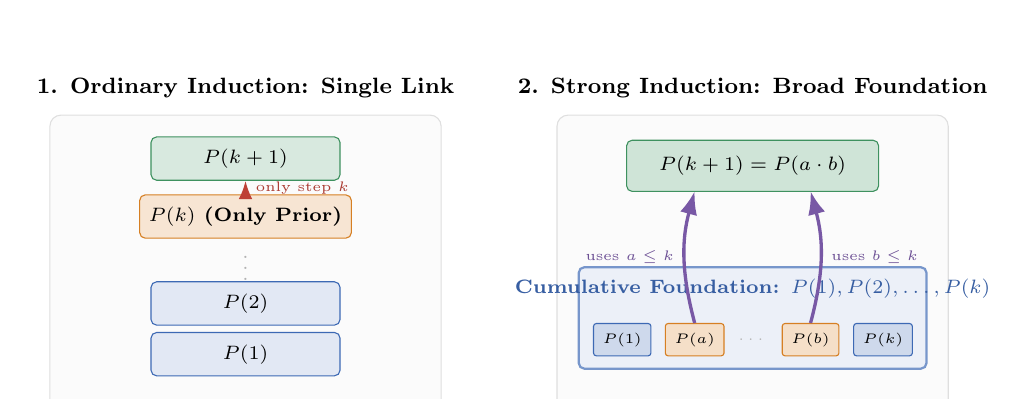
\begin{tikzpicture}[scale=0.92, >=Latex]
  % Panel 1: Ordinary Induction (Single Predecessor)
  \begin{scope}[xshift=0cm]
    \node[anchor=south, font=\footnotesize\bfseries] at (2.4, 3.6) {1. Ordinary Induction: Single Link};
    \draw[rounded corners=4pt, fill=gray!3, draw=gray!25] (-0.3, -0.6) rectangle (5.1, 3.5);
    
    % Blocks
    \node[draw=sourceblue, fill=sourceblue!15, rounded corners=2pt, font=\scriptsize, minimum width=2.4cm, minimum height=0.55cm] (b1) at (2.4, 0.2) {$P(1)$};
    \node[draw=sourceblue, fill=sourceblue!15, rounded corners=2pt, font=\scriptsize, minimum width=2.4cm, minimum height=0.55cm] (b2) at (2.4, 0.9) {$P(2)$};
    \node[font=\scriptsize, text=gray!60] at (2.4, 1.5) {$\vdots$};
    \node[draw=quotientorange, fill=quotientorange!20, rounded corners=2pt, font=\scriptsize\bfseries, minimum width=2.4cm, minimum height=0.55cm] (bk) at (2.4, 2.1) {$P(k)$ (Only Prior)};
    \node[draw=targetgreen, fill=targetgreen!20, rounded corners=2pt, font=\scriptsize\bfseries, minimum width=2.4cm, minimum height=0.55cm] (bk1) at (2.4, 2.9) {$P(k+1)$};
    
    \draw[->, thick, trapred] (bk) -- node[right, font=\tiny, text=trapred!90!black] {only step $k$} (bk1);
  \end{scope}

  % Panel 2: Strong Induction (Cumulative Foundation)
  \begin{scope}[xshift=7.0cm]
    \node[anchor=south, font=\footnotesize\bfseries] at (2.4, 3.6) {2. Strong Induction: Broad Foundation};
    \draw[rounded corners=4pt, fill=gray!3, draw=gray!25] (-0.3, -0.6) rectangle (5.1, 3.5);
    
    % Wide foundation layer
    \draw[thick, sourceblue!70, fill=sourceblue!10, rounded corners=2pt] (0.0, 0.0) rectangle (4.8, 1.4);
    \node[sourceblue!90!black, font=\scriptsize\bfseries] at (2.4, 1.1) {Cumulative Foundation: $P(1), P(2), \dots, P(k)$};
    
    % Sub-blocks inside foundation
    \node[draw=sourceblue, fill=sourceblue!25, rounded corners=1pt, font=\tiny] (p1) at (0.6, 0.4) {$P(1)$};
    \node[draw=quotientorange, fill=quotientorange!25, rounded corners=1pt, font=\tiny\bfseries] (pa) at (1.6, 0.4) {$P(a)$};
    \node[font=\tiny, text=gray!60] at (2.4, 0.4) {$\dots$};
    \node[draw=quotientorange, fill=quotientorange!25, rounded corners=1pt, font=\tiny\bfseries] (pb) at (3.2, 0.4) {$P(b)$};
    \node[draw=sourceblue, fill=sourceblue!25, rounded corners=1pt, font=\tiny] (pk) at (4.2, 0.4) {$P(k)$};
    
    % Target block P(k+1)
    \node[draw=targetgreen, fill=targetgreen!25, rounded corners=2pt, font=\scriptsize\bfseries, minimum width=3.2cm, minimum height=0.65cm] (target) at (2.4, 2.8) {$P(k+1) = P(a \cdot b)$};
    
    % Structural support arrows from a and b
    \draw[->, very thick, structurepurple] (pa.north) to[bend left=15] node[left, font=\tiny, text=structurepurple!90!black] {uses $a \le k$} (1.6, 2.45);
    \draw[->, very thick, structurepurple] (pb.north) to[bend right=15] node[right, font=\tiny, text=structurepurple!90!black] {uses $b \le k$} (3.2, 2.45);
  \end{scope}
\end{tikzpicture}
\end{center}

\subsection{The Principle of Strong Induction}

\begin{theorem}[Principle of Strong Induction]
Let $P(n)$ be a predicate defined for integers $n \ge n_0$. Suppose that:
\begin{enumerate}[label=(\roman*)]
\item \textbf{Base Case:} $P(n_0)$ is true (or several base cases $P(n_0), \dots, P(n_0 + r)$ are true).
\item \textbf{Strong Inductive Step:} For every $k \ge n_0$, if $P(m)$ is true for \textbf{all} integers $m$ satisfying $n_0 \le m \le k$, then $P(k+1)$ is true:
\[
(\forall k \ge n_0)\Big(\big[P(n_0) \land P(n_0 + 1) \land \dots \land P(k)\big] \implies P(k+1)\Big).
\]
\end{enumerate}
Then $P(n)$ is true for all integers $n \ge n_0$.
\end{theorem}

\begin{intuitionbox}
Think of ordinary induction as building a single spire of blocks, where each block balances precarious on top of the one below it. Strong induction builds a masonry wall: block $k+1$ is laid across an entire solid bedrock of prior stones $P(n_0), \dots, P(k)$. When you need to justify step $k+1$, you may draw support from any stone anywhere in the foundation.
\end{intuitionbox}

\subsection{Why Strong Induction Is Not an Extra Axiom}

Is strong induction fundamentally more powerful than ordinary induction? Surprisingly, \textbf{no}. They are logically equivalent.

To see why, define a new predicate $Q(n)$:
\[
Q(n) \iff P(n_0) \land P(n_0 + 1) \land \dots \land P(n).
\]
The statement $Q(n)$ says: ``The property holds for all cases from the beginning up through $n$.'' 

Proving $P$ by strong induction is identical to proving $Q$ by ordinary induction! 
\begin{itemize}
\item Base case: $Q(n_0) \iff P(n_0)$.
\item Inductive step: $Q(k) \implies Q(k+1)$ because $Q(k)$ gives us $P(n_0), \dots, P(k)$, which strong induction uses to deduce $P(k+1)$. Appending $P(k+1)$ to the conjunction yields $Q(k+1)$.
\end{itemize}

Strong induction adds no new logical assumptions to mathematics. It is simply a much more convenient way to package inductive arguments when subproblems jump backward by more than one step.

\subsection{Worked Proof: The Existence of Prime Factorizations}

A positive integer $p \ge 2$ is \emph{prime} if its only positive divisors are $1$ and $p$. An integer $n \ge 2$ that is not prime is \emph{composite}, meaning $n = a \cdot b$ with $2 \le a, b < n$.

\begin{theorem}[Existence of Prime Factorizations]
Every integer $n \ge 2$ can be factored into a product of one or more prime numbers.
\end{theorem}

\begin{proof}
We proceed by strong induction on $n \ge 2$.

\textbf{Base Case ($n = 2$):} The integer $2$ is prime. A single prime is already a product of primes by definition (a product with a single factor). Thus the base case holds.

\textbf{Strong Inductive Step:}
Let $k \ge 2$ be an arbitrary integer. 
Assume that every integer $m$ in the range $2 \le m \le k$ can be factored into a product of primes. (This is our strong induction hypothesis.)

We must now prove that $k+1$ can be factored into a product of primes. We consider two cases:

\begin{itemize}
\item \emph{Case 1: $k+1$ is prime.} If $k+1$ is prime, it is immediately a product of primes (itself), and we are done.
\item \emph{Case 2: $k+1$ is composite.} By definition of composite numbers, there exist integers $a$ and $b$ such that
\[
k + 1 = a \cdot b \quad \text{with} \quad 2 \le a \le k \quad \text{and} \quad 2 \le b \le k.
\]
Because both $a$ and $b$ fall strictly within the range $[2, k]$, our strong induction hypothesis applies to both of them!

Therefore, $a$ can be written as a product of primes:
\[
a = p_1 p_2 \cdots p_r \quad (p_i \text{ prime}),
\]
and $b$ can be written as a product of primes:
\[
b = q_1 q_2 \cdots q_s \quad (q_j \text{ prime}).
\]
Multiplying these two representations together gives:
\[
k + 1 = a \cdot b = (p_1 p_2 \cdots p_r)(q_1 q_2 \cdots q_s).
\]
This exhibits $k+1$ as a product of primes.
\end{itemize}

In both cases, $k+1$ is a product of primes. By the Principle of Strong Induction, every integer $n \ge 2$ is a product of primes.
\end{proof}

\subsection{Connection to Computer Science: Recursive Correctness}

Strong induction is the exact mathematical counterpart to verifying recursive algorithms.

Consider the divide-and-conquer algorithm \texttt{MergeSort}. When sorting a list of size $n$, the algorithm splits the list into two halves of size $\lfloor n/2 \rfloor$ and $\lceil n/2 \rceil$, sorts them recursively, and merges the results.

To prove that \texttt{MergeSort} terminates and produces a correctly sorted array:
\begin{itemize}
\item \textbf{Base Case ($n = 1$):} A single-element list is already sorted.
\item \textbf{Inductive Step:} Assume \texttt{MergeSort} correctly sorts \emph{all} lists of size $m \le k$. To prove it sorts a list of size $k+1$, observe that both halves have size at most $\lceil (k+1)/2 \rceil \le k$. By the strong induction hypothesis, both sub-arrays are sorted correctly. Showing the merge step preserves order completes the proof.
\end{itemize}
Whenever an algorithm makes recursive calls on inputs strictly smaller than the current input, strong induction is the tool that guarantees correctness.

\subsection{What Strong Induction Unlocked, Its Limits, and Where We Go Next}

Strong induction broadens our inductive reach to encompass all of recursive mathematics:
\begin{itemize}
\item \textbf{Number theory:} It gives us the existence of prime factorizations (the bedrock of the Fundamental Theorem of Arithmetic) and the structural properties of integer divisibility.
\item \textbf{Computer science algorithms:} It provides the exact mathematical framework for verifying divide-and-conquer algorithms, dynamic programming recurrences, tree traversals, and structural induction on compiler syntax trees.
\item \textbf{Recurrence relations:} It allows us to solve linear recurrences (like the Fibonacci sequence) where each term depends on multiple earlier steps.
\end{itemize}

Yet both ordinary and strong induction rest on an essential structural assumption: the universe of problems must be **discrete and well-ordered**. 

Induction works on the natural numbers $\N$ because they can be lined up in a single-file, numbered queue: step $1$, step $2$, step $3$, and so on. Every non-empty subset has an identifiable least element that grounds the argument.

What happens, however, when you step outside the discrete world of integers? 
\begin{itemize}
\item Can you line up the dense rational numbers $\Q$ in a sequential queue?
\item Can you line up the continuous real numbers $\R$ in a sequence and do induction from one number to the next?
\item Are all infinite sets organized like $\N$, or are there different magnitudes of infinity that can never be queued up into an inductive list?
\end{itemize}

In Chapter~19, we confront \textbf{Countability and the First Shock of Infinity}, where Georg Cantor shows that while the rationals can surprisingly be threaded into an inductive queue, the continuum of real numbers $\R$ breaks the sequence forever, establishing that some infinities are insurmountable.

\subsection{Exercises}

\begin{enumerate}
\item Prove that every postage amount $n \ge 12$ cents can be formed using only $4$-cent and $5$-cent stamps.
\begin{enumerate}[label=(\alph*)]
\item How many base cases do you need to verify before the induction step takes over? (Hint: Notice that adding a $4$-cent stamp moves from $k-3$ to $k+1$.)
\item Complete the strong induction proof.
\end{enumerate}
\item The Fibonacci numbers are defined by $F_1 = 1$, $F_2 = 1$, and $F_{n+1} = F_n + F_{n-1}$ for $n \ge 2$. Prove by strong induction that
\[
F_n = \frac{1}{\sqrt{5}}\left[\left(\frac{1 + \sqrt{5}}{2}\right)^n - \left(\frac{1 - \sqrt{5}}{2}\right)^n\right] \quad \text{for all } n \ge 1.
\]
\item Prove that any positive integer can be written as a sum of distinct powers of $2$ (existence of binary representations).
\end{enumerate}

\newpage

\section{Countability and the First Shock of Infinity}
\chapterline

For centuries, mathematics treated infinity as a single concept: an endless process, written with the symbol $\infty$.

Then, in the 1870s, Georg Cantor asked a basic question:
\begin{center}
\emph{Can one infinity be strictly larger than another?}
\end{center}

To answer that question, Cantor realized we cannot count an infinite set to its end. Instead, we must return to functions: \textbf{bijective pairing}.

\begin{historybox}
In 1874, Georg Cantor published a paper proving that while the algebraic numbers (roots of polynomials with integer coefficients) can be placed in one-to-one correspondence with the natural numbers $\N$, the real numbers $\R$ cannot. This yielded an unexpected consequence: transcendental numbers like $\pi$ and $e$ were not rare exceptions; they formed an uncountable majority of the continuum.

Cantor's work initially met strong resistance. Leopold Kronecker, a strict finitist who remarked ``God made the integers, all else is human work,'' viewed transfinite numbers skeptically. Henri Poincar\'e famously expressed reservations about transfinite set theory.

In 1891, Cantor introduced his diagonal argument, proving that every set has a strictly larger power set ($|S| < |\pow(S)|$). David Hilbert later championed Cantor's work, declaring in 1926: ``No one shall expel us from the paradise that Cantor has created for us.''
\end{historybox}

\subsection{Measuring Size Without Counting}

Imagine a theater filled with spectators and seats. If every person is sitting in exactly one seat, and no seats are empty, you know with absolute certainty that the number of spectators equals the number of seats. You do not need to count whether there are $50$ people or $50{,}000$; the existence of a bijection proves their quantities match.

Cantor applied this exact principle to infinite sets:

\begin{definition}[Equinumerosity and Countability]
Two sets $A$ and $B$ have the \textbf{same cardinality} (written $|A| = |B|$) if there exists a bijection $f: A \to B$. We say $A$ and $B$ are \textbf{equinumerous}.

A set $S$ is \textbf{countably infinite} if there exists a bijection $f: \N \to S$. A set is \textbf{countable} if it is either finite or countably infinite. A set that is not countable is called \textbf{uncountable}.
\end{definition}

Notice the word \emph{cardinality}: it is simply the mathematician's formal name for the size of a set when measured by pairing. In plain terms, a set is countable if you can line up its elements in an infinite queue:
\[
s_1, \; s_2, \; s_3, \; s_4, \; \dots
\]
such that every single member of the set eventually appears at some finite position in the list.

\begin{recoverybox}
\textbf{Mental Check:} If someone claims a set $S$ is countably infinite, what concrete mathematical object are they obligated to produce?
\par\vspace{0.3em}
\emph{Answer:} An infinite numbered list $s_1, s_2, s_3, \dots$ that contains every single element of $S$ at some finite position $n \in \N$, with no omissions and no duplicates.
\end{recoverybox}

\subsection{Galileo's Paradox: The Evens Match the Naturals}

In 1638, in his final work \emph{Discorsi e dimostrazioni matematiche intorno a due nuove scienze}, Galileo Galilei pointed out a deep riddle about infinite collections. Consider the set of all positive even integers:
\[
2\N = \{2, 4, 6, 8, 10, \dots\}.
\]
Look at them laid out on the number line. Between every two even numbers sits an odd number that was skipped. Our spatial intuition insists there are only half as many even numbers as natural numbers $\N = \{1, 2, 3, \dots\}$.

Yet if we test their cardinality by pairing them up, something startling happens. Consider the function:
\[
f: \N \to 2\N, \quad f(n) = 2n.
\]
\begin{itemize}
\item If $2a = 2b$, then dividing by $2$ gives $a = b$ (injective: no two different counting numbers share the same even partner).
\item Every even integer $2k \in 2\N$ has an input $k \in \N$ where $f(k) = 2k$ (surjective: every even number is claimed).
\end{itemize}
The function $f$ is a bijection. Despite omitting all odd integers, the set of even numbers has the same cardinality as the set of all natural numbers:
\[
|2\N| = |\N|.
\]

\begin{center}
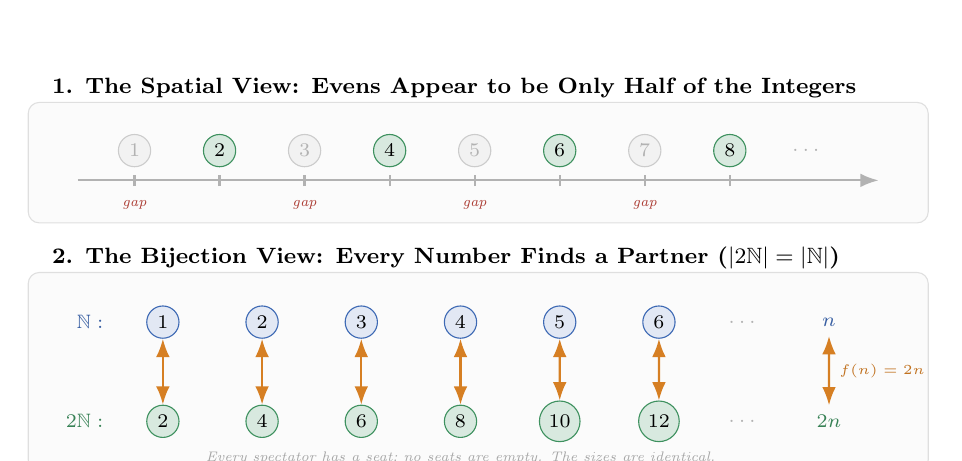
\begin{tikzpicture}[scale=0.90, >=Latex]
  \begin{scope}[yshift=2.2cm]
    \node[anchor=west, font=\footnotesize\bfseries] at (-0.3, 1.3) {1. The Spatial View: Evens Appear to be Only Half of the Integers};
    \draw[rounded corners=4pt, fill=gray!3, draw=gray!25] (-0.5, -0.6) rectangle (12.2, 1.1);
    
    \draw[thick, gray!60, ->] (0.2, 0.0) -- (11.5, 0.0);
    \foreach \x in {1.0, 2.2, 3.4, 4.6, 5.8, 7.0, 8.2, 9.4} {
      \draw[thick, gray!60] (\x, -0.08) -- (\x, 0.08);
    }
    
    \node[circle, draw=gray!40, fill=gray!10, inner sep=2pt, font=\scriptsize, text=gray!60] at (1.0, 0.42) {$1$};
    \node[circle, draw=targetgreen, fill=targetgreen!20, inner sep=2pt, font=\scriptsize\bfseries] at (2.2, 0.42) {$2$};
    \node[circle, draw=gray!40, fill=gray!10, inner sep=2pt, font=\scriptsize, text=gray!60] at (3.4, 0.42) {$3$};
    \node[circle, draw=targetgreen, fill=targetgreen!20, inner sep=2pt, font=\scriptsize\bfseries] at (4.6, 0.42) {$4$};
    \node[circle, draw=gray!40, fill=gray!10, inner sep=2pt, font=\scriptsize, text=gray!60] at (5.8, 0.42) {$5$};
    \node[circle, draw=targetgreen, fill=targetgreen!20, inner sep=2pt, font=\scriptsize\bfseries] at (7.0, 0.42) {$6$};
    \node[circle, draw=gray!40, fill=gray!10, inner sep=2pt, font=\scriptsize, text=gray!60] at (8.2, 0.42) {$7$};
    \node[circle, draw=targetgreen, fill=targetgreen!20, inner sep=2pt, font=\scriptsize\bfseries] at (9.4, 0.42) {$8$};
    \node[font=\scriptsize, text=gray!60] at (10.5, 0.42) {$\dots$};
    
    \node[anchor=north, font=\tiny\itshape, text=trapred!90!black] at (1.0, -0.15) {gap};
    \node[anchor=north, font=\tiny\itshape, text=trapred!90!black] at (3.4, -0.15) {gap};
    \node[anchor=north, font=\tiny\itshape, text=trapred!90!black] at (5.8, -0.15) {gap};
    \node[anchor=north, font=\tiny\itshape, text=trapred!90!black] at (8.2, -0.15) {gap};
  \end{scope}

  \begin{scope}[yshift=-1.2cm]
    \node[anchor=west, font=\footnotesize\bfseries] at (-0.3, 2.3) {2. The Bijection View: Every Number Finds a Partner ($|2\N| = |\N|$)};
    \draw[rounded corners=4pt, fill=gray!3, draw=gray!25] (-0.5, -0.7) rectangle (12.2, 2.1);
    
    \node[anchor=east, font=\scriptsize\bfseries, text=sourceblue!90!black] at (0.7, 1.4) {$\N:$};
    \node[circle, draw=sourceblue, fill=sourceblue!15, inner sep=2pt, font=\scriptsize\bfseries] (n1) at (1.4, 1.4) {$1$};
    \node[circle, draw=sourceblue, fill=sourceblue!15, inner sep=2pt, font=\scriptsize\bfseries] (n2) at (2.8, 1.4) {$2$};
    \node[circle, draw=sourceblue, fill=sourceblue!15, inner sep=2pt, font=\scriptsize\bfseries] (n3) at (4.2, 1.4) {$3$};
    \node[circle, draw=sourceblue, fill=sourceblue!15, inner sep=2pt, font=\scriptsize\bfseries] (n4) at (5.6, 1.4) {$4$};
    \node[circle, draw=sourceblue, fill=sourceblue!15, inner sep=2pt, font=\scriptsize\bfseries] (n5) at (7.0, 1.4) {$5$};
    \node[circle, draw=sourceblue, fill=sourceblue!15, inner sep=2pt, font=\scriptsize\bfseries] (n6) at (8.4, 1.4) {$6$};
    \node[font=\scriptsize, text=gray!60] (ndots) at (9.6, 1.4) {$\dots$};
    \node[font=\scriptsize, text=sourceblue!90!black] (nn) at (10.8, 1.4) {$n$};

    \node[anchor=east, font=\scriptsize\bfseries, text=targetgreen!90!black] at (0.7, 0.0) {$2\N:$};
    \node[circle, draw=targetgreen, fill=targetgreen!20, inner sep=2pt, font=\scriptsize\bfseries] (e1) at (1.4, 0.0) {$2$};
    \node[circle, draw=targetgreen, fill=targetgreen!20, inner sep=2pt, font=\scriptsize\bfseries] (e2) at (2.8, 0.0) {$4$};
    \node[circle, draw=targetgreen, fill=targetgreen!20, inner sep=2pt, font=\scriptsize\bfseries] (e3) at (4.2, 0.0) {$6$};
    \node[circle, draw=targetgreen, fill=targetgreen!20, inner sep=2pt, font=\scriptsize\bfseries] (e4) at (5.6, 0.0) {$8$};
    \node[circle, draw=targetgreen, fill=targetgreen!20, inner sep=2pt, font=\scriptsize\bfseries] (e5) at (7.0, 0.0) {$10$};
    \node[circle, draw=targetgreen, fill=targetgreen!20, inner sep=2pt, font=\scriptsize\bfseries] (e6) at (8.4, 0.0) {$12$};
    \node[font=\scriptsize, text=gray!60] (edots) at (9.6, 0.0) {$\dots$};
    \node[font=\scriptsize, text=targetgreen!90!black] (en) at (10.8, 0.0) {$2n$};

    \draw[<->, thick, quotientorange] (n1) -- (e1);
    \draw[<->, thick, quotientorange] (n2) -- (e2);
    \draw[<->, thick, quotientorange] (n3) -- (e3);
    \draw[<->, thick, quotientorange] (n4) -- (e4);
    \draw[<->, thick, quotientorange] (n5) -- (e5);
    \draw[<->, thick, quotientorange] (n6) -- (e6);
    \draw[<->, thick, quotientorange] (nn) -- node[right, font=\tiny\bfseries, text=quotientorange!90!black] {$f(n) = 2n$} (en);

    \node[anchor=north, font=\tiny\itshape, text=gray!70] at (5.6, -0.3) {Every spectator has a seat; no seats are empty. The sizes are identical.};
  \end{scope}
\end{tikzpicture}
\end{center}

For infinite sets, Euclid's classical common notion ``the whole is greater than the part'' ceases to hold. In fact, Richard Dedekind took this as the very defining property of the infinite: \emph{a set $S$ is infinite if and only if it can be placed in one-to-one correspondence with a proper subset of itself.} For any finite set, the Pigeonhole Principle guarantees that removing an element strictly decreases the size; for an infinite set, you can remove infinitely many elements and still have just as many left over.

\begin{recoverybox}
\textbf{Mental Check:} Can you construct an explicit bijection between the natural numbers $\N$ and the positive \emph{odd} integers $\{1, 3, 5, 7, \dots\}$?
\par\vspace{0.3em}
\emph{Answer:} Yes! The function $g(n) = 2n - 1$ sends $1 \mapsto 1$, $2 \mapsto 3$, $3 \mapsto 5$, pairing every natural number with a unique odd number.
\end{recoverybox}

\subsection{The Integers are Countable}

What about the set of all integers $\Z = \{\dots, -3, -2, -1, 0, 1, 2, 3, \dots\}$? 

Unlike $\N$, which begins cleanly at $1$, the integers stretch endlessly in two opposite directions. If you tried to count them by walking out along the positives $0, 1, 2, 3, \dots$, you would walk forever and never reach $-1$. 

The solution is to weave the two directions together, alternating between positive and negative values:

\begin{center}
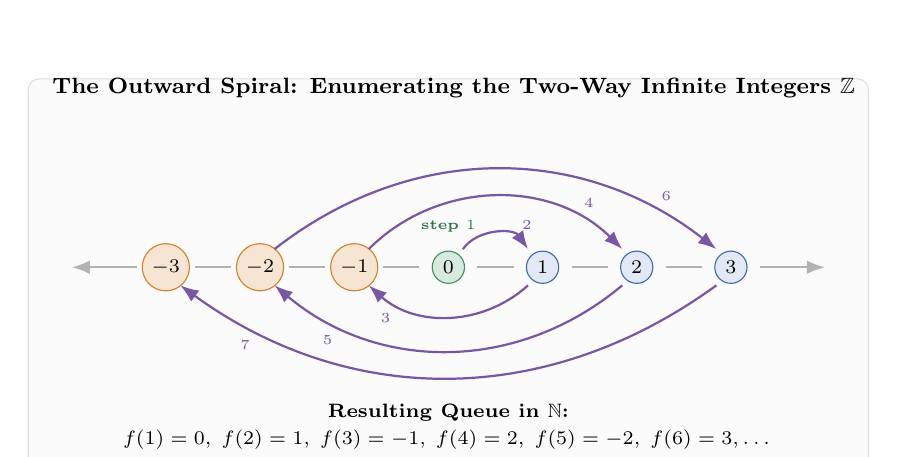
\begin{tikzpicture}[scale=0.92, >=Latex]
  \draw[rounded corners=4pt, fill=gray!3, draw=gray!25] (-5.8, -2.8) rectangle (5.8, 2.6);
  \node[anchor=south west, font=\footnotesize\bfseries] at (-5.6, 2.2) {The Outward Spiral: Enumerating the Two-Way Infinite Integers $\Z$};

  % Integer line segments between nodes (no line passing through any text)
  \draw[thick, gray!60, <-] (-5.2, 0.0) -- (-4.3, 0.0);
  \draw[thick, gray!60] (-3.5, 0.0) -- (-3.0, 0.0);
  \draw[thick, gray!60] (-2.2, 0.0) -- (-1.7, 0.0);
  \draw[thick, gray!60] (-0.9, 0.0) -- (-0.4, 0.0);
  \draw[thick, gray!60] (0.4, 0.0) -- (0.9, 0.0);
  \draw[thick, gray!60] (1.7, 0.0) -- (2.2, 0.0);
  \draw[thick, gray!60] (3.0, 0.0) -- (3.5, 0.0);
  \draw[thick, gray!60, ->] (4.3, 0.0) -- (5.2, 0.0);
  
  \node[circle, draw=targetgreen, fill=targetgreen!20, inner sep=2pt, font=\scriptsize\bfseries] (z0) at (0, 0) {$0$};
  \node[circle, draw=sourceblue, fill=sourceblue!15, inner sep=2pt, font=\scriptsize\bfseries] (zp1) at (1.3, 0) {$1$};
  \node[circle, draw=quotientorange, fill=quotientorange!20, inner sep=2pt, font=\scriptsize\bfseries] (zm1) at (-1.3, 0) {$-1$};
  \node[circle, draw=sourceblue, fill=sourceblue!15, inner sep=2pt, font=\scriptsize\bfseries] (zp2) at (2.6, 0) {$2$};
  \node[circle, draw=quotientorange, fill=quotientorange!20, inner sep=2pt, font=\scriptsize\bfseries] (zm2) at (-2.6, 0) {$-2$};
  \node[circle, draw=sourceblue, fill=sourceblue!15, inner sep=2pt, font=\scriptsize\bfseries] (zp3) at (3.9, 0) {$3$};
  \node[circle, draw=quotientorange, fill=quotientorange!20, inner sep=2pt, font=\scriptsize\bfseries] (zm3) at (-3.9, 0) {$-3$};
  
  % Step 1: at 0
  \node[anchor=south, font=\tiny\bfseries, text=targetgreen!80!black] at (0, 0.35) {step $1$};
  
  % Step 2: 0 -> +1 (arc above)
  \draw[->, thick, structurepurple] (0.2, 0.25) to[bend left=55] node[pos=0.75, above right=-1pt, font=\tiny\bfseries, text=structurepurple] {$2$} (1.1, 0.25);
  
  % Step 3: +1 -> -1 (arc below)
  \draw[->, thick, structurepurple] (1.1, -0.25) to[bend left=42] node[pos=0.8, below left=-1pt, font=\tiny\bfseries, text=structurepurple] {$3$} (-1.1, -0.25);
  
  % Step 4: -1 -> +2 (arc above)
  \draw[->, thick, structurepurple] (-1.1, 0.25) to[bend left=45] node[pos=0.8, above right=-1pt, font=\tiny\bfseries, text=structurepurple] {$4$} (2.4, 0.25);
  
  % Step 5: +2 -> -2 (arc below)
  \draw[->, thick, structurepurple] (2.4, -0.25) to[bend left=40] node[pos=0.8, below left=-1pt, font=\tiny\bfseries, text=structurepurple] {$5$} (-2.4, -0.25);
  
  % Step 6: -2 -> +3 (arc above)
  \draw[->, thick, structurepurple] (-2.4, 0.25) to[bend left=38] node[pos=0.85, above right=-1pt, font=\tiny\bfseries, text=structurepurple] {$6$} (3.7, 0.25);
  
  % Step 7: +3 -> -3 (arc below)
  \draw[->, thick, structurepurple] (3.7, -0.25) to[bend left=36] node[pos=0.85, below left=-1pt, font=\tiny\bfseries, text=structurepurple] {$7$} (-3.7, -0.25);

  % Bottom queue representation
  \node[anchor=north, font=\scriptsize, align=center] at (0, -1.75) {
    \textbf{Resulting Queue in $\N$:}\\[0.25em]
    $f(1)=0, \; f(2)=1, \; f(3)=-1, \; f(4)=2, \; f(5)=-2, \; f(6)=3, \dots$
  };
\end{tikzpicture}\\[0.5em]
{\small\textbf{Figure 19.2:}\label{19:fig-integers-spiral} \emph{The outward spiral bijection between $\N$ and $\Z$. Walking in a single direction would abandon all negative numbers. By spiraling outward from $0$ in alternating steps ($+1, -1, +2, -2, \dots$), every integer is reached at a predictable, finite index, proving $|\Z| = |\N|$.}}
\end{center}
The explicit bijection $f: \N \to \Z$ is:
\[
f(n) = \begin{cases} \frac{n}{2} & \text{if } n \text{ is even}, \\ -\frac{n-1}{2} & \text{if } n \text{ is odd}. \end{cases}
\]
To verify that this really is a bijection, we can write down its exact inverse $f^{-1}: \Z \to \N$. If you hand me any integer $z$, I can instantly tell you its position $n$ in line:
\[
f^{-1}(z) = \begin{cases} 2z & \text{if } z > 0, \\ 1 - 2z & \text{if } z \le 0. \end{cases}
\]
For example, the integer $-3$ appears at index $1 - 2(-3) = 7$, exactly matching our table. Every integer appears at a predictable, finite index. Thus $|\Z| = |\N|$: the two-way infinite line has no more elements than the one-way ray!

\subsection{The Rationals are Countable: Cantor's Snake}

The rational numbers $\Q$ seem much larger than the integers. Between any two integers lies an infinite collection of fractions. Even more strikingly, between any two fractions $a < b$, you can always find another fraction sitting between them---for instance, their midpoint $(a+b)/2$. And between that midpoint and either end, there are still more fractions, ad infinitum. 

Unlike the integers, where $4$ is followed immediately by $5$ with nothing in between, the rationals have no ``next-door neighbor.'' If you stand at $1/2$, what is the next rational number? There is no such thing! Mathematicians say the rational numbers are \textbf{dense} on the real line. 

If you try to list the rationals in increasing numerical order, there are infinitely many fractions between $0$ and $1$, so you would never even reach $2$.

Yet density is a topological property describing how numbers are arranged in space, not a measure of cardinality: the rationals are countable.

To see why, Cantor realized we must abandon the number line entirely. Instead of ordering fractions by their numerical value, arrange all pairs of positive integers $(p, q)$ in an infinite two-dimensional grid, where $p$ is the row (the numerator) and $q$ is the column (the denominator). We then weave through the grid along finite diagonals:

\begin{center}
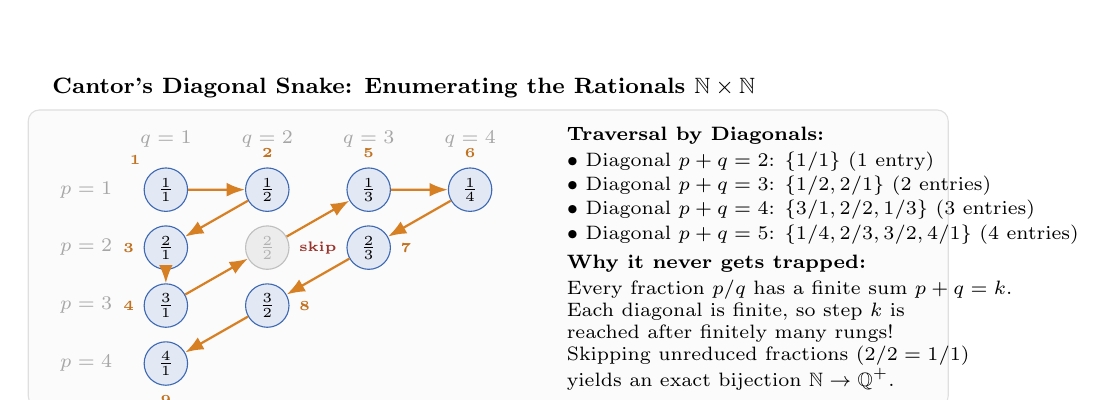
\begin{tikzpicture}[scale=0.92, >=Latex]
  \node[anchor=west, font=\footnotesize\bfseries] at (-0.3, 3.8) {Cantor's Diagonal Snake: Enumerating the Rationals $\N \times \N$};
  \draw[rounded corners=4pt, fill=gray!3, draw=gray!25] (-0.5, -0.6) rectangle (12.2, 3.5);
  
  % Column labels
  \node[font=\scriptsize\bfseries, text=gray!70] at (1.4, 3.1) {$q=1$};
  \node[font=\scriptsize\bfseries, text=gray!70] at (2.8, 3.1) {$q=2$};
  \node[font=\scriptsize\bfseries, text=gray!70] at (4.2, 3.1) {$q=3$};
  \node[font=\scriptsize\bfseries, text=gray!70] at (5.6, 3.1) {$q=4$};
  
  % Row labels
  \node[font=\scriptsize\bfseries, text=gray!70] at (0.3, 2.4) {$p=1$};
  \node[font=\scriptsize\bfseries, text=gray!70] at (0.3, 1.6) {$p=2$};
  \node[font=\scriptsize\bfseries, text=gray!70] at (0.3, 0.8) {$p=3$};
  \node[font=\scriptsize\bfseries, text=gray!70] at (0.3, 0.0) {$p=4$};
  
  % Nodes
  \node[circle, draw=sourceblue, fill=sourceblue!15, inner sep=2pt, font=\scriptsize] (f11) at (1.4, 2.4) {$\frac{1}{1}$};
  \node[circle, draw=sourceblue, fill=sourceblue!15, inner sep=2pt, font=\scriptsize] (f12) at (2.8, 2.4) {$\frac{1}{2}$};
  \node[circle, draw=sourceblue, fill=sourceblue!15, inner sep=2pt, font=\scriptsize] (f13) at (4.2, 2.4) {$\frac{1}{3}$};
  \node[circle, draw=sourceblue, fill=sourceblue!15, inner sep=2pt, font=\scriptsize] (f14) at (5.6, 2.4) {$\frac{1}{4}$};

  \node[circle, draw=sourceblue, fill=sourceblue!15, inner sep=2pt, font=\scriptsize] (f21) at (1.4, 1.6) {$\frac{2}{1}$};
  \node[circle, draw=gray!50, fill=gray!15, inner sep=2pt, font=\scriptsize, text=gray!60] (f22) at (2.8, 1.6) {$\frac{2}{2}$};
  \node[circle, draw=sourceblue, fill=sourceblue!15, inner sep=2pt, font=\scriptsize] (f23) at (4.2, 1.6) {$\frac{2}{3}$};

  \node[circle, draw=sourceblue, fill=sourceblue!15, inner sep=2pt, font=\scriptsize] (f31) at (1.4, 0.8) {$\frac{3}{1}$};
  \node[circle, draw=sourceblue, fill=sourceblue!15, inner sep=2pt, font=\scriptsize] (f32) at (2.8, 0.8) {$\frac{3}{2}$};

  \node[circle, draw=sourceblue, fill=sourceblue!15, inner sep=2pt, font=\scriptsize] (f41) at (1.4, 0.0) {$\frac{4}{1}$};
  
  % Order Badges
  \node[font=\tiny\bfseries, text=quotientorange!90!black, anchor=south east] at (f11.north west) {1};
  \node[font=\tiny\bfseries, text=quotientorange!90!black, anchor=south] at (f12.north) {2};
  \node[font=\tiny\bfseries, text=quotientorange!90!black, anchor=east] at (f21.west) {3};
  \node[font=\tiny\bfseries, text=quotientorange!90!black, anchor=east] at (f31.west) {4};
  \node[font=\tiny\bfseries, text=trapred!80!black, anchor=west] at (f22.east) {skip};
  \node[font=\tiny\bfseries, text=quotientorange!90!black, anchor=south] at (f13.north) {5};
  \node[font=\tiny\bfseries, text=quotientorange!90!black, anchor=south] at (f14.north) {6};
  \node[font=\tiny\bfseries, text=quotientorange!90!black, anchor=west] at (f23.east) {7};
  \node[font=\tiny\bfseries, text=quotientorange!90!black, anchor=west] at (f32.east) {8};
  \node[font=\tiny\bfseries, text=quotientorange!90!black, anchor=north] at (f41.south) {9};
  
  % Snake traversal arrows
  \draw[->, thick, quotientorange] (f11) -- (f12);
  \draw[->, thick, quotientorange] (f12) -- (f21);
  \draw[->, thick, quotientorange] (f21) -- (f31);
  \draw[->, thick, quotientorange] (f31) -- (f22);
  \draw[->, thick, quotientorange] (f22) -- (f13);
  \draw[->, thick, quotientorange] (f13) -- (f14);
  \draw[->, thick, quotientorange] (f14) -- (f23);
  \draw[->, thick, quotientorange] (f23) -- (f32);
  \draw[->, thick, quotientorange] (f32) -- (f41);
  
  % Side panel description
  \node[anchor=west, font=\scriptsize, align=left] at (6.8, 1.45) {
    \textbf{Traversal by Diagonals:}\\[0.15em]
    $\bullet$ Diagonal $p+q = 2$: $\{1/1\}$ (1 entry)\\[0.1em]
    $\bullet$ Diagonal $p+q = 3$: $\{1/2, 2/1\}$ (2 entries)\\[0.1em]
    $\bullet$ Diagonal $p+q = 4$: $\{3/1, 2/2, 1/3\}$ (3 entries)\\[0.1em]
    $\bullet$ Diagonal $p+q = 5$: $\{1/4, 2/3, 3/2, 4/1\}$ (4 entries)\\[0.35em]
    \textbf{Why it never gets trapped:}\\[0.15em]
    Every fraction $p/q$ has a finite sum $p+q = k$.\\
    Each diagonal is finite, so step $k$ is\\
    reached after finitely many rungs!\\
    Skipping unreduced fractions ($2/2 = 1/1$)\\
    yields an exact bijection $\N \to \Q^+$.
  };
\end{tikzpicture}\\[0.5em]
{\small\textbf{Figure 19.3:}\label{19:fig-cantor-snake} \emph{Cantor's diagonal snake enumerating the positive rationals $\Q^+$. By weaving along finite diagonals $p+q = k$, every fraction is reached after finitely many steps, proving that the dense rationals are countable ($|\Q| = |\N|$).}}
\end{center}

Because each diagonal $p + q = k$ contains only $k - 1$ entries (a finite number), the snake reaches any chosen fraction $p/q$ after a finite number of steps. For instance, the fraction $355/113$ sits on diagonal $355 + 113 = 468$; because all previous $466$ diagonals together contain only finitely many fractions, the snake arrives at $355/113$ after finitely many steps.

By omitting duplicate fractions that are not in lowest terms (such as $2/2 = 1/1$, $4/2 = 2/1$, or $2/4 = 1/2$), each positive rational number is visited exactly once. This establishes an explicit bijection between $\N$ and the positive rationals $\Q^+$.

Just as we did with the integers, we can now interleave the positive rationals with their negative counterparts and insert $0$ at the very front:
\[
0, \; \frac{1}{1}, \; -\frac{1}{1}, \; \frac{1}{2}, \; -\frac{1}{2}, \; \frac{2}{1}, \; -\frac{2}{1}, \; \frac{1}{3}, \; -\frac{1}{3}, \; \dots
\]
Every rational number in existence appears at a definite, finite position. Therefore:
\[
|\Q| = |\N|.
\]
Density does not make a set uncountable: even though fractions are densely packed along the number line, the set of all rational numbers can be arranged into a single infinite sequence.

\begin{recoverybox}
\textbf{Mental Check:} Why can't we count the grid by reading row 1 all the way across: $1/1, 1/2, 1/3, 1/4, \dots$?
\par\vspace{0.3em}
\emph{Answer:} Because row 1 is infinite! If you tried to finish row 1 before moving to row 2, you would walk forever along row 1 and never reach $2/1$. The diagonal snake works because every diagonal is finite.
\end{recoverybox}

\subsection{The Shock: The Real Numbers are Uncountable}

At this point, one might wonder: is \emph{every} infinite set countable? If both the integers and the dense set of rational numbers can be arranged into sequences, could it be that all infinite sets have the same cardinality?

Cantor showed that the answer is no: the real numbers cannot be listed in an infinite sequence.

\begin{theorem}[Cantor's Diagonal Theorem]
The open interval of real numbers $(0, 1)$ is uncountable.
\end{theorem}

\begin{center}
\begin{tikzpicture}[scale=0.92, >=Latex]
  \node[anchor=west, font=\footnotesize\bfseries] at (-0.3, 4.3) {Cantor's Diagonal Construction: A Real Missing from the Catalog};
  \draw[rounded corners=4pt, fill=gray!3, draw=gray!25] (-0.5, -0.8) rectangle (12.2, 4.0);
  
  % Rows of cataloged reals
  \node[font=\footnotesize\bfseries, text=sourceblue!90!black] at (0.8, 3.2) {$r_1 = 0.$};
  \node[draw=quotientorange, fill=quotientorange!25, rounded corners=1pt, inner sep=2pt, font=\footnotesize\bfseries] at (2.0, 3.2) {$7$};
  \node[font=\footnotesize] at (2.6, 3.2) {$1$};
  \node[font=\footnotesize] at (3.2, 3.2) {$4$};
  \node[font=\footnotesize] at (3.8, 3.2) {$2$};
  \node[font=\footnotesize] at (4.4, 3.2) {$8$};
  \node[font=\footnotesize, text=gray!50] at (5.2, 3.2) {$\dots$};

  \node[font=\footnotesize\bfseries, text=sourceblue!90!black] at (0.8, 2.5) {$r_2 = 0.$};
  \node[font=\footnotesize] at (2.0, 2.5) {$3$};
  \node[draw=quotientorange, fill=quotientorange!25, rounded corners=1pt, inner sep=2pt, font=\footnotesize\bfseries] at (2.6, 2.5) {$5$};
  \node[font=\footnotesize] at (3.2, 2.5) {$9$};
  \node[font=\footnotesize] at (3.8, 2.5) {$2$};
  \node[font=\footnotesize] at (4.4, 2.5) {$6$};
  \node[font=\footnotesize, text=gray!50] at (5.2, 2.5) {$\dots$};

  \node[font=\footnotesize\bfseries, text=sourceblue!90!black] at (0.8, 1.8) {$r_3 = 0.$};
  \node[font=\footnotesize] at (2.0, 1.8) {$0$};
  \node[font=\footnotesize] at (2.6, 1.8) {$8$};
  \node[draw=quotientorange, fill=quotientorange!25, rounded corners=1pt, inner sep=2pt, font=\footnotesize\bfseries] at (3.2, 1.8) {$3$};
  \node[font=\footnotesize] at (3.8, 1.8) {$3$};
  \node[font=\footnotesize] at (4.4, 1.8) {$3$};
  \node[font=\footnotesize, text=gray!50] at (5.2, 1.8) {$\dots$};

  \node[font=\footnotesize\bfseries, text=sourceblue!90!black] at (0.8, 1.1) {$r_4 = 0.$};
  \node[font=\footnotesize] at (2.0, 1.1) {$4$};
  \node[font=\footnotesize] at (2.6, 1.1) {$1$};
  \node[font=\footnotesize] at (3.2, 1.1) {$9$};
  \node[draw=quotientorange, fill=quotientorange!25, rounded corners=1pt, inner sep=2pt, font=\footnotesize\bfseries] at (3.8, 1.1) {$4$};
  \node[font=\footnotesize] at (4.4, 1.1) {$0$};
  \node[font=\footnotesize, text=gray!50] at (5.2, 1.1) {$\dots$};

  % Divider
  \draw[thick, gray!40] (0.2, 0.6) -- (5.6, 0.6);

  % Constructed rebel number d
  \node[font=\footnotesize\bfseries, text=targetgreen!90!black] at (0.8, 0.1) {$d \; = 0.$};
  \node[draw=targetgreen, fill=targetgreen!25, rounded corners=1pt, inner sep=2pt, font=\footnotesize\bfseries] at (2.0, 0.1) {$4$};
  \node[draw=targetgreen, fill=targetgreen!25, rounded corners=1pt, inner sep=2pt, font=\footnotesize\bfseries] at (2.6, 0.1) {$4$};
  \node[draw=targetgreen, fill=targetgreen!25, rounded corners=1pt, inner sep=2pt, font=\footnotesize\bfseries] at (3.2, 0.1) {$4$};
  \node[draw=targetgreen, fill=targetgreen!25, rounded corners=1pt, inner sep=2pt, font=\footnotesize\bfseries] at (3.8, 0.1) {$5$};
  \node[font=\footnotesize, text=gray!50] at (5.2, 0.1) {$\dots$};

  % Callout text
  \node[anchor=west, font=\scriptsize, align=left] at (6.0, 1.8) {
    $\bullet$ Diagonal digits $d_{nn}$ shown in orange.\\[0.5em]
    $\bullet$ Constructed digit $c_n$ (in green):\\
    \quad $c_n = 5$ if $d_{nn} = 4$; otherwise $c_n = 4$.\\[0.6em]
    $\bullet$ By construction, $d$ differs from $r_n$ at position $n$.\\[0.5em]
    $\bullet$ Hence $d \neq r_n$ for every $n$: $d$ is not on the list!
  };
\end{tikzpicture}\\[0.5em]
{\small\textbf{Figure 19.4:}\label{19:fig-cantor-diagonal} \emph{Cantor's diagonal construction. Given any purported list $r_1, r_2, \dots$ of all reals in $(0, 1)$, we construct a real number $d$ whose $n$-th digit differs from the diagonal digit $d_{nn}$. Since $d$ differs from $r_n$ at digit $n$ for every $n$, $d$ cannot appear on the list, proving $(0, 1)$ is uncountable.}}
\end{center}

\begin{proof}
We argue by contradiction. Suppose that $(0, 1)$ were countable. 
Then there exists a bijection from $\N$ to $(0, 1)$, meaning we can write down a complete, numbered catalog listing every real number in $(0, 1)$:
\[
r_1, \; r_2, \; r_3, \; r_4, \; \dots
\]
Let us express each number in its infinite decimal expansion:
\begin{align*}
r_1 &= 0.\mathbf{d_{11}} d_{12} d_{13} d_{14} \dots \\
r_2 &= 0.d_{21} \mathbf{d_{22}} d_{23} d_{24} \dots \\
r_3 &= 0.d_{31} d_{32} \mathbf{d_{33}} d_{34} \dots \\
r_4 &= 0.d_{41} d_{42} d_{43} \mathbf{d_{44}} \dots
\end{align*}
where $d_{ij} \in \{0, 1, \dots, 9\}$ is the $j$-th decimal digit of $r_i$.

We now construct a real number $d = 0.c_1 c_2 c_3 c_4 \dots$ that differs from every number on the list. For each integer $n \ge 1$, we inspect the diagonal digit $d_{nn}$ and choose $c_n$ according to the simple rule:
\[
c_n = \begin{cases} 5 & \text{if } d_{nn} = 4, \\ 4 & \text{if } d_{nn} \neq 4. \end{cases}
\]
Notice three properties of this constructed number $d$:
\begin{enumerate}[label=\arabic*.]
\item Because every digit $c_n$ is strictly either $4$ or $5$, $0 < d < 1$. Thus $d \in (0, 1)$.
\item The decimal expansion of $d$ contains only $4$s and $5$s, avoiding trailing infinite sequences of $0$s or $9$s. Its decimal representation is strictly unique.
\item Compare $d$ to any number $r_n$ on the list: their $n$-th decimal digits differ by construction ($c_n \neq d_{nn}$). Therefore:
\[
d \neq r_n \quad \text{for every integer } n \ge 1.
\]
\end{enumerate}

This is a direct contradiction! The list $r_1, r_2, \dots$ was assumed to contain \emph{every} real number in $(0, 1)$, yet the number $d$ lives in $(0, 1)$ and appears nowhere on the list.

Therefore, our initial assumption was false. The interval $(0, 1)$ cannot be listed in a sequence, and is uncountable.
\end{proof}

\begin{trapbox}
\textbf{The Trap of Dual Decimal Expansions}

Why did we strictly restrict our choices to the digits $4$ and $5$? Why not simply set $c_n = d_{nn} + 1 \pmod{10}$?

Because in base-10 arithmetic, some numbers possess \emph{two} distinct decimal representations:
\[
0.49999\dots = 0.50000\dots
\]
If our construction produced a number ending in infinite trailing $9$s (or infinite trailing $0$s), an argument could be raised that $d$ equals a listed number with an alternate representation (such as $0.4999\dots = 0.5000\dots$).

By choosing every digit $c_n$ strictly from $\{4, 5\}$, the number $d$ never ends in trailing $9$s or trailing $0$s. Its decimal expansion is unique, ensuring that $d \neq r_n$ holds unambiguously.
\end{trapbox}

Since $(0, 1) \subseteq \R$, the full set of real numbers $\R$ must also be uncountable. There are multiple, distinct tiers of infinity:
\[
|\N| = |\Z| = |\Q| < |\R|.
\]

\subsection{What Cardinality Unlocked, Its Limits, and Where We Go Next}

Cantor's cardinality theory led to fundamental developments across mathematics:
\begin{itemize}
\item \textbf{Non-constructive existence:} An \emph{algebraic number} is any root of a polynomial with integer coefficients (such as $\sqrt{2}$ or $-3/5$). Because polynomials of degree $n$ have only finitely many roots, and there are only countably many integer polynomials, the set of algebraic numbers is countable. But $\R$ is uncountable! This means the \emph{transcendental numbers} (numbers like $\pi$ and $e$ that cannot be solved by integer polynomials) must be uncountably infinite. Cantor proved that almost all real numbers are transcendental without constructing a single explicit example.
\item \textbf{The foundations of computing:} In 1936, Alan Turing used Cantor's diagonal argument to prove that the Halting Problem is uncomputable. Because computer programs (and Turing machines) are finite strings of text written in a finite alphabet, there are only countably many computer programs ($\aleph_0$). However, there are uncountably many mathematical functions from $\N$ to $\{0, 1\}$ ($2^{\aleph_0}$). Thus, the vast majority of problems can never be solved by any algorithm!
\item \textbf{The transfinite hierarchy:} Cantor proved that for \emph{any} set $S$, the power set $\pow(S)$ always has strictly greater cardinality than $S$ ($|S| < |\pow(S)|$). This established an infinite hierarchy of transfinite cardinalities: $\aleph_0 < 2^{\aleph_0} < 2^{2^{\aleph_0}} < \dots$, showing there is no maximal cardinality.
\end{itemize}

Yet cardinality does not capture geometric or topological structure. 

It counts elements by bijection, but does not distinguish dimension or distance. Consider this surprising fact, also discovered by Cantor:
\[
|(0, 1)| = |\R| = |\R^2| = |\R^{100}|.
\]
An interval, the real line, a two-dimensional plane, and a 100-dimensional space all have the same cardinality. When Cantor proved in 1877 that a line segment can be mapped bijectively to a unit square by interleaving digits, he famously wrote to Richard Dedekind:
\begin{center}
\emph{``Je le vois, mais je ne le crois pas!''} (``I see it, but I do not believe it!'')
\end{center}

\begin{center}
\begin{tikzpicture}[scale=0.92, >=Latex]
  \draw[rounded corners=4pt, fill=gray!3, draw=gray!25] (-5.5, -1.2) rectangle (5.5, 2.4);
  \node[anchor=south west, font=\footnotesize\bfseries] at (-5.3, 2.0) {Geometric Bijection: Projecting a Finite Interval to the Infinite Line $\R$};

  % Center of projection
  \coordinate (C) at (0, 1.5);
  \fill[targetgreen!80!black] (C) circle (2pt);
  \node[above=2pt, font=\scriptsize\bfseries, text=targetgreen!80!black] at (C) {Center of Projection $P$};

  % Bounded semicircular arc
  \draw[very thick, sourceblue] (-0.97, 1.24) arc[start angle=195, end angle=345, radius=1.0];
  \draw[fill=white, draw=sourceblue, thick] (-0.97, 1.24) circle (1.8pt);
  \draw[fill=white, draw=sourceblue, thick] (0.97, 1.24) circle (1.8pt);
  \node[anchor=west, font=\tiny\bfseries, text=sourceblue] at (1.1, 1.1) {interval $(-\pi/2, \pi/2)$};

  % Infinite real line
  \draw[thick, gray!70, <->] (-5.0, -0.4) -- (5.0, -0.4);
  \node[above=2pt, font=\scriptsize\bfseries, text=gray!80!black] at (4.7, -0.4) {$\R$};

  % Projection rays
  \draw[dashed, structurepurple!70!black] (C) -- (0, -0.4);
  \draw[dashed, structurepurple!70!black] (C) -- (1.58, -0.4);
  \draw[dashed, structurepurple!70!black] (C) -- (3.33, -0.4);
  \draw[dashed, structurepurple!70!black] (C) -- (-1.58, -0.4);
  \draw[dashed, structurepurple!70!black] (C) -- (-3.33, -0.4);

  % Points on arc
  \fill[sourceblue] (0, 0.5) circle (1.5pt);
  \fill[sourceblue] (0.64, 0.73) circle (1.5pt);
  \fill[sourceblue] (0.87, 1.00) circle (1.5pt);
  \fill[sourceblue] (-0.64, 0.73) circle (1.5pt);
  \fill[sourceblue] (-0.87, 1.00) circle (1.5pt);

  % Points on line
  \fill[targetgreen!80!black] (0, -0.4) circle (1.6pt) node[below=1pt, font=\tiny\bfseries] {$0$};
  \fill[targetgreen!80!black] (1.58, -0.4) circle (1.6pt) node[below=1pt, font=\tiny\bfseries] {$x_1$};
  \fill[targetgreen!80!black] (3.33, -0.4) circle (1.6pt) node[below=1pt, font=\tiny\bfseries] {$x_2$};
  \fill[targetgreen!80!black] (-1.58, -0.4) circle (1.6pt) node[below=1pt, font=\tiny\bfseries] {$-x_1$};
  \fill[targetgreen!80!black] (-3.33, -0.4) circle (1.6pt) node[below=1pt, font=\tiny\bfseries] {$-x_2$};

  \node[anchor=south, font=\tiny\itshape, text=structurepurple!90!black] at (0, -1.05) {Each ray through angle $\theta$ hits exactly one point $x = \tan\theta$, giving $|(-\pi/2, \pi/2)| = |\R|$.};
\end{tikzpicture}\\[0.5em]
{\small\textbf{Figure 19.5:}\label{19:fig-interval-to-real-line} \emph{Stereographic projection establishing equinumerosity $|(-\pi/2, \pi/2)| = |\R|$. Bending the open interval into an arc and casting rays from the center $P$ matches each angle $\theta$ with exactly one real number $x = \tan\theta$. The bounded interval has the exact same cardinality as the infinite real line.}}
\end{center}

Yet a plane is topologically and geometrically different from a line, and spaces of different dimensions possess distinct geometric properties. Cardinality does not detect dimension, distance, or continuity: it cannot determine whether a function is continuous or whether a sequence of points converges.

To do calculus and analysis, we cannot rely on cardinality alone. We must equip the continuum with a notion of distance and limits. In Chapter~20, we turn to \textbf{Real Analysis Preview: Epsilon as a Contract}, showing how Cauchy and Weierstrass formalized limits using quantifier definitions.

\subsection{Exercises}

\begin{enumerate}
\item \textbf{Mental Check: Finite Strings vs Infinite Sequences.}
Let $\Sigma = \{0, 1\}$.
\begin{enumerate}[label=(\alph*)]
\item Prove that the set of all \emph{finite} binary strings $\Sigma^*$ (strings of length $0, 1, 2, \dots$) is countably infinite. (Hint: List the empty string, then strings of length $1$, then strings of length $2$, and so on.)
\item Prove that the set of all \emph{infinite} binary sequences $\Sigma^\omega = \{(b_1, b_2, b_3, \dots) : b_i \in \{0, 1\}\}$ is uncountable by adapting Cantor's diagonal argument.
\end{enumerate}

\item \textbf{Rescaling the Continuum.}
\begin{enumerate}[label=(\alph*)]
\item For any two real numbers $a < b$, construct an explicit linear bijection $f: (0, 1) \to (a, b)$, proving that all open intervals have the same cardinality regardless of their length.
\item Using the tangent function, construct an explicit bijection $g: (-\pi/2, \pi/2) \to \R$, proving that a finite interval of length $\pi$ has the exact same cardinality as the entire infinite real line.
\end{enumerate}

\item \textbf{Countable Union of Countable Sets.}
Suppose $\{A_n\}_{n=1}^\infty$ is a countably infinite collection of sets, where each set $A_n = \{a_{n,1}, a_{n,2}, a_{n,3}, \dots\}$ is countably infinite. Prove that their union:
\[
A = \bigcup_{n=1}^\infty A_n
\]
is countably infinite. (Hint: Arrange the elements into a two-dimensional grid where row $n$ lists the elements of $A_n$, and adapt Cantor's diagonal snake traversal.)

\item \textbf{Cantor's General Theorem: Diagonalization in the Abstract.}
Prove that for \emph{any} set $S$ (finite or infinite), there is no surjective function from $S$ to its power set $\pow(S)$.
\begin{enumerate}[label=(\alph*)]
\item Suppose towards a contradiction that $f: S \to \pow(S)$ is surjective. Define the subset:
\[
D = \{x \in S : x \notin f(x)\}.
\]
\item Because $f$ is surjective and $D \in \pow(S)$, there must exist an element $d \in S$ such that $f(d) = D$.
\item Ask the critical question: Is $d \in D$? Show that $d \in D \implies d \notin D$, and $d \notin D \implies d \in D$, producing a contradiction.
\item Reflect: How is the definition of $D$ related to Cantor's diagonal number $d$, Russell's paradox, and the Halting Problem?
\end{enumerate}

\item \textbf{A Glimpse of Hilbert's Hotel on the Continuum.}
Prove that the half-open interval $(0, 1]$ has the exact same cardinality as the open interval $(0, 1)$ by constructing an explicit bijection $h: (0, 1] \to (0, 1)$.
\par\vspace{0.2em}
\emph{Hint:} Isolate a countable sequence in $(0, 1]$, say $S = \{1, 1/2, 1/4, \dots, 1/2^k, \dots\}$. Shift each element of $S$ to the next power of $2$ ($1 \mapsto 1/2$, $1/2 \mapsto 1/4$, $\dots$), and leave every other real number $x \notin S$ exactly where it is!
\end{enumerate}

\newpage

\section{Real Analysis Preview: Epsilon as a Contract}
\chapterline

In introductory calculus, we are told that a sequence approaches a limit:
\[
\lim_{n \to \infty} a_n = L,
\]
or that a function approaches a value:
\[
\lim_{x \to c} f(x) = L.
\]
Textbooks describe this dynamically: ``As $x$ gets closer and closer to $c$, $f(x)$ gets closer and closer to $L$.''

While that mental picture is intuitive, it lacks logical teeth. What does ``closer and closer'' actually mean? Does it mean the sequence can never drift backward? Does it mean the distance decreases at every single step? 

In the nineteenth century, mathematicians like Augustin-Louis Cauchy and Karl Weierstrass realized that if mathematics was to rest on solid bedrock, motion had to be replaced by logic. They reframed the limit not as a physical journey, but as an \textbf{ironclad adversarial contract}.

\begin{historybox}
The rigor of real analysis was born out of a scathing philosophical attack. In 1734, Bishop George Berkeley published \emph{The Analyst: A Discourse Addressed to an Infidel Mathematician}. Berkeley attacked Isaac Newton's ``fluxions'' and Gottfried Leibniz's ``differentials,'' pointing out a glaring logical contradiction in early calculus: to compute a derivative, one divided by an increment $\Delta x$ (which requires $\Delta x \neq 0$), only to declare $\Delta x = 0$ a moment later to make unwanted terms vanish. Berkeley famously scoffed:
\begin{quote}
\itshape
``And what are these same evanescent increments? They are neither finite quantities, nor quantities infinitely small, nor yet nothing. May we not call them the ghosts of departed quantities?''
\end{quote}
For nearly a century, mathematicians calculated brilliant results using these ``ghosts,'' yet lacked a defensible logical foundation. The breakthrough came when Augustin-Louis Cauchy (\emph{Cours d'Analyse}, 1821) and Karl Weierstrass in his 1860s Berlin lectures abolished infinitesimals entirely. Weierstrass realized that calculus does not require quantities that are mysteriously ``infinitely small.'' Instead, a limit is a static game played with ordinary, positive real numbers ($\eps$ and $\delta$) governed by nested quantifiers.
\end{historybox}

\subsection{The Adversarial Game: Sequences}

\begin{definition}[Limit of a Sequence]
A sequence of real numbers $(a_n)_{n=1}^\infty$ \textbf{converges} to a real number $L$, written $\lim_{n \to \infty} a_n = L$, if:
\[
(\forall \eps > 0)(\exists N \in \N)(\forall n \in \N)(n \ge N \implies |a_n - L| < \eps).
\]
\end{definition}

\subsection{Plain English}

No matter how narrow a vertical tolerance band $(L - \eps, L + \eps)$ someone draws around $L$, you can walk far enough out along the sequence—past some cutoff index $N$—that every term from $a_N$ onward stays trapped inside that band forever. Conversely, if a sequence like $a_n = (-1)^n$ keeps jumping between $+1$ and $-1$, then as soon as $\eps \le 1$, no horizontal band of half-height $\eps$ can trap both values, so terms keep escaping no matter how far out you go.

\subsection{Who Chooses What?}

To master this definition, view it as a two-player game between a \textbf{Challenger} (the skeptic) and a \textbf{Prover} (you):
\begin{enumerate}[label=\arabic*.]
\item \textbf{The Challenger's Move ($\forall \eps > 0$):} The challenger goes first and picks an error tolerance $\eps > 0$. Because they want to expose a flaw in your claim, they may choose $\eps$ as tiny as they please—say, $\eps = 0.00001$.
\item \textbf{Your Move ($\exists N \in \N$):} After seeing their $\eps$, you inspect the formula for $a_n$ and produce a finite index cutoff $N \in \N$. Because you move second, your choice of $N$ is allowed to depend on $\eps$.
\item \textbf{The Challenger's Inspection ($\forall n \ge N$):} The challenger is now free to test \emph{any} index $n \ge N$ at or past your cutoff—including the worst-case boundary term $n = N$—and you win the round only if $|a_n - L| < \eps$ holds for every single $n \ge N$:
\[
L - \eps < a_n < L + \eps.
\]
\end{enumerate}

If you have a formula or strategy that produces a winning cutoff $N(\eps)$ against \emph{every possible} positive tolerance $\eps$ the challenger can name, the sequence converges to $L$.

\begin{center}
\begin{tikzpicture}[scale=0.90, >=Latex]
  % Lane 1: Sequence Epsilon Corridor
  \begin{scope}[yshift=0cm]
    \node[anchor=west, font=\small\bfseries] at (-0.5, 3.6) {1. The Sequence Contract: $\forall \eps > 0, \exists N \in \N, \forall n \ge N, |a_n - L| < \eps$};
    \draw[rounded corners=4pt, fill=gray!3, draw=gray!25] (-0.6, -0.6) rectangle (12.2, 3.4);
    
    % Shaded tolerance band
    \fill[targetgreen!12] (0.2, 1.0) rectangle (11.6, 2.2);
    \draw[thick, dashed, targetgreen!80] (0.2, 2.2) -- (11.6, 2.2) node[right, font=\tiny\bfseries, text=targetgreen!90!black] {$L + \eps$};
    \draw[thick, sourceblue!90!black] (0.2, 1.6) -- (11.6, 1.6) node[right, font=\tiny\bfseries, text=sourceblue!90!black] {Limit $L$};
    \draw[thick, dashed, targetgreen!80] (0.2, 1.0) -- (11.6, 1.0) node[right, font=\tiny\bfseries, text=targetgreen!90!black] {$L - \eps$};
    
    % Threshold N line
    \draw[very thick, trapred!80, dashed] (5.0, 0.0) -- (5.0, 3.0) node[above, font=\scriptsize\bfseries, text=trapred!90!black] {Cutoff $N$};
    
    % Sequence points
    % Before N (oscillating outside band)
    \node[circle, fill=sourceblue, inner sep=1.8pt, label={above:\tiny $a_1$}] at (0.8, 2.8) {};
    \node[circle, fill=sourceblue, inner sep=1.8pt, label={below:\tiny $a_2$}] at (1.6, 0.4) {};
    \node[circle, fill=sourceblue, inner sep=1.8pt, label={above:\tiny $a_3$}] at (2.4, 2.5) {};
    \node[circle, fill=sourceblue, inner sep=1.8pt, label={below:\tiny $a_4$}] at (3.3, 0.7) {};
    \node[circle, fill=sourceblue, inner sep=1.8pt, label={above:\tiny $a_5$}] at (4.2, 2.3) {};
    
    % After N (trapped forever inside band)
    \node[circle, fill=targetgreen!80!black, inner sep=1.8pt, label={above:\tiny $a_N$}] at (5.3, 1.9) {};
    \node[circle, fill=targetgreen!80!black, inner sep=1.8pt] at (6.2, 1.35) {};
    \node[circle, fill=targetgreen!80!black, inner sep=1.8pt] at (7.1, 1.75) {};
    \node[circle, fill=targetgreen!80!black, inner sep=1.8pt] at (8.0, 1.48) {};
    \node[circle, fill=targetgreen!80!black, inner sep=1.8pt] at (8.9, 1.68) {};
    \node[circle, fill=targetgreen!80!black, inner sep=1.8pt] at (9.8, 1.55) {};
    \node[circle, fill=targetgreen!80!black, inner sep=1.8pt] at (10.7, 1.62) {};
    
    \node[font=\scriptsize, align=left, text=targetgreen!90!black] at (8.5, 0.3) {All terms trapped inside $\eps$-tube for $n \ge N$};
  \end{scope}

  % Lane 2: Function Epsilon-Delta Box
  \begin{scope}[yshift=-4.8cm]
    \node[anchor=west, font=\small\bfseries] at (-0.5, 3.8) {2. The Function Contract: $\forall \eps > 0, \exists \delta > 0, 0 < |x - c| < \delta \implies |f(x) - L| < \eps$};
    \draw[rounded corners=4pt, fill=gray!3, draw=gray!25] (-0.6, -0.6) rectangle (12.2, 3.6);
    
    % Axes
    \draw[->, thick, gray!60] (0.5, 0.2) -- (8.5, 0.2) node[right, font=\scriptsize] {$x$};
    \draw[->, thick, gray!60] (1.0, 0.0) -- (1.0, 3.2) node[above, font=\scriptsize] {$y$};
    
    % Shaded safe rectangle (delta x epsilon)
    \fill[targetgreen!15] (3.4, 0.8) rectangle (5.8, 2.4);
    \draw[thick, draw=targetgreen!70] (3.4, 0.8) rectangle (5.8, 2.4);
    
    % Limits and deltas
    % Horizontal epsilon band
    \draw[dashed, targetgreen!80] (1.0, 2.4) node[left, font=\tiny] {$L+\eps$} -- (8.0, 2.4);
    \draw[dashed, sourceblue!80] (1.0, 1.6) node[left, font=\tiny\bfseries] {$L$} -- (8.0, 1.6);
    \draw[dashed, targetgreen!80] (1.0, 0.8) node[left, font=\tiny] {$L-\eps$} -- (8.0, 0.8);
    
    % Vertical delta band
    \draw[dashed, quotientorange!80] (3.4, 0.2) node[below, font=\tiny] {$c-\delta$} -- (3.4, 2.8);
    \draw[dashed, sourceblue!80] (4.6, 0.2) node[below, font=\tiny\bfseries] {$c$} -- (4.6, 2.8);
    \draw[dashed, quotientorange!80] (5.8, 0.2) node[below, font=\tiny] {$c+\delta$} -- (5.8, 2.8);
    
    % Center point (c, L)
    \node[circle, fill=sourceblue, inner sep=2pt] at (4.6, 1.6) {};
    
    % Curve y = f(x) passing safely through vertical sides
    \draw[very thick, structurepurple] (2.0, 0.3) to[out=25, in=215] (3.4, 1.0) to[out=35, in=215] (4.6, 1.6) to[out=35, in=205] (5.8, 2.2) to[out=25, in=200] (7.5, 2.9);
    \node[structurepurple!90!black, font=\scriptsize\bfseries] at (7.8, 2.9) {$y=f(x)$};
    
    % Annotations
    \node[anchor=west, font=\scriptsize, align=left] at (8.7, 1.6) {
      $\bullet$ Skeptic dictates height $\pm\eps$.\\
      $\bullet$ Prover responds with width $\pm\delta$.\\
      $\bullet$ Curve exits through the \textbf{vertical}\\
      \quad boundaries, never the $\eps$-ceiling\\
      \quad or $\eps$-floor!
    };
  \end{scope}
\end{tikzpicture}
\end{center}

\subsection{Worked Proof: \texorpdfstring{$1/n \to 0$}{1/n -> 0}}

\begin{theorem}
\[
\lim_{n \to \infty} \frac{1}{n} = 0.
\]
\end{theorem}

\begin{proof}
Let $\eps > 0$ be arbitrary. 

\emph{Scratchpad Search:} We want $|a_n - L| < \eps$, which means:
\[
\left|\frac{1}{n} - 0\right| = \frac{1}{n} < \eps \iff n > \frac{1}{\eps}.
\]
This tells us exactly how far out in the sequence we need to travel.

\emph{Official Written Proof:}
By the Archimedean Property of real numbers, there exists a positive integer $N \in \N$ such that
\[
N > \frac{1}{\eps}.
\]
Now let $n \in \N$ be an arbitrary index and assume $n \ge N$.
Because $n \ge N$, taking reciprocals reverses the inequality:
\[
\frac{1}{n} \le \frac{1}{N}.
\]
Combining this with our choice of $N > 1/\eps$ (which means $1/N < \eps$):
\[
\left|\frac{1}{n} - 0\right| = \frac{1}{n} \le \frac{1}{N} < \eps.
\]
Thus for all $n \ge N$, $|1/n - 0| < \eps$. Since $\eps > 0$ was arbitrary, $\lim_{n \to \infty} 1/n = 0$.
\end{proof}

\subsection{The Continuous Contract: Epsilon and Delta}

The exact same game governs continuous functions, with one twist: instead of choosing an integer index cutoff $N$, you choose an input neighborhood radius $\delta > 0$.

\begin{definition}[Continuity at a Point]
A function $f: \R \to \R$ is \textbf{continuous at a point $c \in \R$} if:
\[
(\forall \eps > 0)(\exists \delta > 0)(\forall x \in \R)(|x - c| < \delta \implies |f(x) - f(c)| < \eps).
\]
\end{definition}

Geometrically, the skeptic draws a horizontal strip of half-height $\eps$ centered at $y = f(c)$. You respond by constructing a vertical window of half-width $\delta$ centered at $x = c$. You win if the graph of $f(x)$ stays trapped within the skeptic's strip across the entire width of your window.

\begin{theorem}
The linear function $f(x) = 3x + 2$ is continuous at every $c \in \R$.
\end{theorem}

\begin{proof}
Let $c \in \R$ and $\eps > 0$ be arbitrary.

\emph{Scratchpad Search:} Because $f(x) = 3x + 2$ has slope $3$, any horizontal input deviation $|x - c|$ is stretched vertically by a factor of $3$:
\[
|f(x) - f(c)| = |(3x + 2) - (3c + 2)| = 3|x - c| < \eps \iff |x - c| < \frac{\eps}{3}.
\]
This tells us to divide the output tolerance by the slope and set $\delta = \eps / 3$.

\emph{Official Proof:}
Choose $\delta = \frac{\eps}{3} > 0$. Suppose $|x - c| < \delta$. Then:
\[
|f(x) - f(c)| = |(3x + 2) - (3c + 2)| = 3|x - c| < 3\delta = 3\left(\frac{\eps}{3}\right) = \eps.
\]
Thus $f$ is continuous at $c$.
\end{proof}

\subsection{Why Analysis Is Proof Training}

Real analysis has a reputation for being demanding, but its difficulty rarely comes from complicated arithmetic. Its challenge lies in \textbf{quantifier order} and tracking which variables are allowed to depend on which earlier choices. Notice how for the linear function $f(x) = 3x + 2$, the slope is $3$ everywhere, so $\delta = \eps/3$ works at every point $c$. For a curved graph like $f(x) = x^2$, the slope $f'(c) = 2c$ grows steeper as $c$ moves to the right—meaning a fixed vertical band $\pm\eps$ forces a narrower and narrower horizontal window $\delta$ as $c$ increases, so $\delta$ must depend on both $\eps$ and $c$.

Notice the strict dependency chain:
\[
\forall \eps > 0 \quad \longrightarrow \quad \exists N \in \N \quad \longrightarrow \quad \forall n \ge N.
\]
Your choice of $N$ is permitted to depend on $\eps$. It is \emph{not} permitted to depend on $n$, because $n$ has not been introduced yet!

If you swap the order of the first two quantifiers:
\[
\exists N \in \N \quad \forall \eps > 0 \quad \forall n \ge N \dots
\]
you would be claiming that a single fixed cutoff $N$ works for \emph{every} tolerance simultaneously. If a sequence is trapped within $\eps = 10^{-100}$ past index $N$ for all $\eps$, every term past $N$ must equal $L$ exactly! Swapping two words in the quantifier prefix transforms a subtle statement about convergence into a trivial statement about sequences that become constant.

When you practice $\eps$-$N$ and $\eps$-$\delta$ proofs, you are not just learning analysis. You are training your logical reflexes to respect the scoping, dependencies, and rules of formal mathematical thought.

\begin{trapbox}
\textbf{Cauchy's Great Quantifier Slip (1821):}
Even the greatest pioneers stumbled when navigating quantifier order. In his 1821 textbook \emph{Cours d'Analyse}, Cauchy stated as an established theorem that if an infinite series of continuous functions converges, its sum must also be continuous. 
Five years later, Niels Henrik Abel and others showed this was false: a series of smooth trigonometric waves can converge to a square wave with vertical cliff edges and jump discontinuities! 
What had gone wrong? Cauchy had assumed that because each individual point $x$ eventually settles down ($\forall x \, \forall \eps > 0 \, \exists N$), the whole curve must settle down at a single shared speed ($\forall \eps > 0 \, \exists N \, \forall x$). He accidentally swapped the order of ``for every $x$'' and ``there exists a cutoff $N$''! It took over two decades for Philipp Ludwig von Seidel (1847) and George Gabriel Stokes to untangle this confusion, giving birth to the modern distinction between pointwise and uniform convergence.
\end{trapbox}

\subsection{What Analysis Unlocked, Its Limits, and Where We Go Next}

The $\eps$-$\delta$ revolution provided the rock-solid bedrock that saved calculus from collapse:
\begin{itemize}
\item \textbf{Calculus without contradiction:} Derivatives, integrals, and the Fundamental Theorem of Calculus were finally proved without invoking vanishing ghosts or dividing by zero.
\item \textbf{Infinite series discipline:} It allowed mathematicians to analyze power series, Fourier transforms, and wave equations without producing divergent absurdities.
\item \textbf{Logical precision:} It trained generations of mathematicians in quantifier scoping, variable binding, and adversarial proof construction.
\end{itemize}

Yet we must acknowledge where the $\eps$-$\delta$ contract encounters its boundary: it is fundamentally tethered to the **metric ruler of the real line**. 

The definitions of $|x - c| < \delta$ and $|f(x) - L| < \eps$ rely on measuring physical distances with absolute values. But in modern physics and geometry, we frequently study spaces where:
\begin{itemize}
\item There is no coordinate grid and no ruler measuring distances (such as curved spacetimes in general relativity).
\item Spaces can be bent, stretched, or compressed elastically without tearing (topology).
\item Spaces are defined algebraically by symmetries and group actions rather than numbers.
\end{itemize}
If you stretch a rubber sheet, every distance between points changes---meaning all $\eps$ and $\delta$ values are altered---yet the underlying continuity of the surface has not been broken at all! Tying continuity to a ruler is an artificial restriction.

This brings us to the threshold of advanced pure mathematics! In the chapters ahead:
\begin{itemize}
\item In Chapter~21, \textbf{Abstract Algebra Preview: Structure and Symmetry}, we step beyond numbers to study groups, rings, and fields---the algebraic languages of symmetry and lawful transformation.
\item In Chapter~22, \textbf{Topology Preview: Continuity Without Rulers}, we liberate continuity from $\eps$ and $\delta$ forever, learning how to define open sets and nearness using the pure preimage machinery of Chapter~14.
\item In Chapters~28 and 35, we will return to analysis for a deep second pass, exploring uniform convergence, Dedekind cuts, and compactness.
\end{itemize}

\subsection{Exercises}

\begin{enumerate}
\item Use the formal $\eps$-$N$ definition of a limit to prove:
\[
\lim_{n \to \infty} \frac{2n + 1}{n + 3} = 2.
\]
(Perform your scratchpad algebra first to isolate $|a_n - 2|$, bound the denominator cleanly, and then write the official proof.)
\item Prove that the sequence $a_n = (-1)^n$ does \emph{not} converge to $1$. 
(To negate the limit definition: show there exists an $\eps > 0$ such that for every $N \in \N$, there is some $n \ge N$ with $|a_n - 1| \ge \eps$.)
\item Use the $\eps$-$\delta$ definition to prove that $f(x) = x^2$ is continuous at $c = 3$. (Hint: Factor $|x^2 - 9| = |x - 3||x + 3|$, assume $\delta \le 1$ to bound $|x + 3|$, and choose $\delta = \min\{1, \eps/7\}$.)
\end{enumerate}

\newpage

\section{Abstract Algebra Preview: Structure and Symmetry}
\chapterline

\subsection{The 300-year quest: how polynomial roots forced a revolution}

For nearly three centuries after Scipione del Ferro, Niccol\`o Tartaglia, and Gerolamo Cardano discovered the general formula for cubic equations in 1545, and Lodovico Ferrari solved the quartic, algebra was defined by a single obsession: find the algebraic formula for the roots of a fifth-degree equation (the general quintic):
\[
a x^5 + b x^4 + c x^3 + d x^2 + e x + f = 0.
\]
The greatest minds of Europe---Leonhard Euler, Joseph-Louis Lagrange, and Carl Friedrich Gauss---attempted to crack the quintic using radicals ($\sqrt[n]{\cdot}$) and arithmetic operations. Every attempt hit an impenetrable barrier: substituting variables to eliminate terms invariably generated auxiliary equations (resolvents) of degree six or higher, making the problem harder, not easier.

Why did three hundred years of algebraic genius fail? Because algebra was asking the wrong question.

In May 1832, on the eve of a fatal duel at the age of twenty, a young French revolutionary named \'{E}variste Galois spent his final night scribbling frantic mathematical notes to his friend Auguste Chevalier. Galois realized that the solvability of an equation has nothing to do with clever algebraic substitutions or the numerical values of coefficients. Instead, it is governed entirely by the \emph{symmetries of its roots under permutation}.

Galois asked: if you shuffle the roots of a polynomial around, which shuffles preserve all algebraic relations among those roots? He called this collection of shuffles a \textbf{group}. Two decades later, in 1854, the English mathematician Arthur Cayley realized that Galois's insight transcended polynomials: a group is not merely an arrangement of roots or numbers, but an abstract universe of symmetries governed by purely relational operational laws.

\subsection{Geometric symmetry: the equilateral triangle}

To see what Galois and Cayley saw without getting lost in fifth-degree polynomials, consider an equilateral triangle sitting on a table.

You can perform operations on this triangle that leave it looking completely undisturbed. You can rotate it by $120^\circ$, rotate it by $240^\circ$, or leave it entirely alone (a rotation by $0^\circ$). You can also pick it up, flip it over across any of its three axes of symmetry, and set it back down.

\begin{center}
\begin{tikzpicture}[scale=1.1, line join=round, >=Latex]
  % Equilateral triangle
  \coordinate (O) at (0, 0);
  \coordinate (A) at (90:2.4);
  \coordinate (B) at (210:2.4);
  \coordinate (C) at (330:2.4);

  % Shaded interior
  \fill[sourceblue!12] (A) -- (B) -- (C) -- cycle;
  \draw[thick, sourceblue] (A) -- (B) -- (C) -- cycle;

  % Center
  \fill[structurepurple] (O) circle (2pt) node[below right=2pt, font=\small, text=structurepurple] {$O$};

  % Vertices
  \fill[sourceblue] (A) circle (2.5pt) node[above=4pt, font=\bfseries] {$1$};
  \fill[sourceblue] (B) circle (2.5pt) node[below left=4pt, font=\bfseries] {$2$};
  \fill[sourceblue] (C) circle (2.5pt) node[below right=4pt, font=\bfseries] {$3$};

  % Reflection axes (dashed lines)
  \draw[dashed, quotientorange, thick] (90:2.8) -- (270:1.6) node[below, font=\small, text=quotientorange] {$s_1$ (axis through $1$)};
  \draw[dashed, targetgreen, thick] (210:2.8) -- (30:1.6) node[above right, font=\small, text=targetgreen] {$s_2$ (axis through $2$)};
  \draw[dashed, trapred, thick] (330:2.8) -- (150:1.6) node[above left, font=\small, text=trapred] {$s_3$ (axis through $3$)};

  % Rotation arrow around center
  \draw[->, thick, structurepurple] (50:0.9) arc (50:190:0.9) node[midway, above left, font=\small, text=structurepurple] {$r = +120^\circ$};
\end{tikzpicture}
\end{center}

In elementary mathematics, the focus is on the triangle itself: its side lengths, its angles, its area. In abstract algebra, the spotlight shifts entirely away from the shape and onto the collection of \emph{operations} that preserve the shape.

The objects of study are not numbers. They are the transformations themselves:
\[
\{e, r, r^2, s_1, s_2, s_3\}
\]
where $e$ is the do-nothing identity, $r$ is counterclockwise rotation by $120^\circ$, $r^2$ is rotation by $240^\circ$, and $s_1, s_2, s_3$ are reflections across the three altitude lines.

What can you do with two transformations? You can perform one after the other. That composition is an algebraic operation:
\[
a \cdot b = \text{``do } b \text{ first, then do } a\text{''}.
\]
When you compose two symmetries of the triangle, the result is always another symmetry of the triangle. If you rotate by $120^\circ$ and then rotate by $120^\circ$, you get a $240^\circ$ rotation. If you reflect across $s_1$ and then rotate, the vertices land in a configuration identical to having performed a single reflection across a different axis.

\subsection{The algebraic axioms of a group}

When mathematicians abstracted this behavior across geometry, number systems, and polynomial roots, they extracted four fundamental properties that make the algebra work.

\begin{definition}
A \textbf{group} is a set $G$ equipped with a binary operation $\cdot : G \times G \to G$ satisfying four axioms:
\begin{enumerate}
\item \textbf{Closure}: For all $a, b \in G$, the product $a \cdot b$ belongs to $G$.
\item \textbf{Associativity}: For all $a, b, c \in G$, $(a \cdot b) \cdot c = a \cdot (b \cdot c)$.
\item \textbf{Identity}: There exists an element $e \in G$ such that for all $a \in G$,
\[
e \cdot a = a \cdot e = a.
\]
\item \textbf{Inverses}: For each $a \in G$, there exists an element $b \in G$ such that
\[
a \cdot b = b \cdot a = e.
\]
We denote this inverse $b$ by $a^{-1}$.
\end{enumerate}
\end{definition}

Notice that commutativity ($a \cdot b = b \cdot a$) is \emph{not} on the list. In our triangle example, try holding the triangle, flipping it across $s_1$, and then rotating by $120^\circ$. Now reset the triangle and do the operations in the opposite order: rotate by $120^\circ$ first, and then flip across $s_1$. The corners end up in different positions! The group of symmetries of the triangle, denoted $D_3$ (the dihedral group of order 6), is non-abelian: the order of operations matters.

\begin{center}
\begin{tikzpicture}[scale=0.9, >=Latex]
  % Cayley Table snippet showing non-commutativity
  \node[font=\bfseries] at (0, 3.2) {Multiplication Table for Rotations and Reflections};

  % Grid background
  \draw[thick, gray!40] (-3, -1.8) grid[step=1.2] (3, 2.6);

  % Header Row
  \node[font=\bfseries, text=structurepurple] at (-2.4, 2.0) {$\cdot$};
  \node[font=\bfseries] at (-1.2, 2.0) {$e$};
  \node[font=\bfseries, text=structurepurple] at (0.0, 2.0) {$r$};
  \node[font=\bfseries, text=quotientorange] at (1.2, 2.0) {$s_1$};
  \node[font=\bfseries] at (2.4, 2.0) {$s_2$};

  % Header Column
  \node[font=\bfseries] at (-2.4, 0.8) {$e$};
  \node[font=\bfseries, text=structurepurple] at (-2.4, -0.4) {$r$};
  \node[font=\bfseries, text=quotientorange] at (-2.4, -1.6) {$s_1$};

  % Highlight cell r * s_1 = s_3
  \fill[quotientorange!20, rounded corners=2pt] (0.6, -1.0) rectangle (1.8, 0.2);
  \node[font=\bfseries, text=quotientorange] at (1.2, -0.4) {$s_3$};

  % Highlight cell s_1 * r = s_2
  \fill[trapred!20, rounded corners=2pt] (-0.6, -2.2) rectangle (0.6, -1.0);
  \node[font=\bfseries, text=trapred] at (0.0, -1.6) {$s_2$};

  % Other sample entries
  \node at (-1.2, 0.8) {$e$};
  \node at (0.0, 0.8) {$r$};
  \node at (1.2, 0.8) {$s_1$};
  \node at (2.4, 0.8) {$s_2$};

  \node at (-1.2, -0.4) {$r$};
  \node at (0.0, -0.4) {$r^2$};
  \node at (2.4, -0.4) {$s_1$};

  \node at (-1.2, -1.6) {$s_1$};
  \node at (2.4, -1.6) {$r$};

  % Annotations explaining non-commutativity
  \node[right=12pt, align=left, font=\small] at (3.2, 0.4) {
    $\mathbf{r \cdot s_1 = s_3}$ \\
    $\mathbf{s_1 \cdot r = s_2}$ \\[4pt]
    Since $s_3 \neq s_2$, we have: \\
    \textcolor{trapred}{\textbf{$r \cdot s_1 \neq s_1 \cdot r$}}. \\
    Order of operations matters!
  };
\end{tikzpicture}
\end{center}

\subsection{Examples across mathematics}

Once you have this definition, you begin recognizing groups in widely different settings:
\begin{itemize}
\item \textbf{Integers under addition} $(\Z, +)$: The identity is $0$, the inverse of $n$ is $-n$, and addition is associative. Notice this is an abelian group because $a+b = b+a$.
\item \textbf{Nonzero rational numbers under multiplication} $(\Q \setminus \{0\}, \cdot)$: The identity is $1$, and the inverse of $p/q$ is $q/p$. (The number $0$ must be removed because it has no multiplicative inverse.)
\item \textbf{Invertible $n \times n$ real matrices} $\mathrm{GL}_n(\R)$ under matrix multiplication: The identity is the $n \times n$ identity matrix $I$, every invertible matrix has an inverse $A^{-1}$, and matrix multiplication is associative. For $n \ge 2$, matrix multiplication is non-commutative.
\item \textbf{Permutations of a finite set} $S_n$: The set of all bijections from $\{1, 2, \dots, n\}$ to itself under function composition.
\end{itemize}

\subsection{Proving theorems purely from the axioms}

The true beauty of abstract algebra is that when you prove a theorem using only the group axioms, your conclusion is guaranteed to hold in every single group that exists, without needing to re-prove it for integers, matrices, or geometric rotations.

\begin{theorem}
In any group $G$, the identity element is unique.
\end{theorem}

\begin{proof}
Suppose $e$ and $e'$ are both identity elements in $G$.
Because $e$ is an identity element, multiplying it by any element leaves that element unchanged. In particular, for the element $e'$, we have:
\[
e \cdot e' = e'.
\]
On the other hand, because $e'$ is also an identity element, multiplying any element by $e'$ leaves that element unchanged. Applying this to the element $e$, we have:
\[
e \cdot e' = e.
\]
Comparing these two equations gives:
\[
e = e \cdot e' = e'.
\]
Therefore, $e = e'$. There cannot be two distinct identity elements.
\end{proof}

\begin{theorem}
In any group $G$, each element has a unique inverse.
\end{theorem}

\begin{proof}
Let $a \in G$, and suppose that both $b$ and $c$ satisfy the definition of an inverse for $a$. That means:
\[
a \cdot b = b \cdot a = e \quad \text{and} \quad a \cdot c = c \cdot a = e.
\]
We examine the expression $c \cdot a \cdot b$. By associativity, we can group this product in two different ways:
\[
(c \cdot a) \cdot b = c \cdot (a \cdot b).
\]
Now substitute our knowledge of inverses into each side:
\begin{align*}
(c \cdot a) \cdot b &= e \cdot b = b, \\
c \cdot (a \cdot b) &= c \cdot e = c.
\end{align*}
Equating the two results gives $b = c$. The inverse of $a$ is unique.
\end{proof}

\begin{intuitionbox}
Trace what happened in that proof. We did not appeal to negative numbers, division, or geometric reflections. We used only associativity and the definition of the identity element. The associative property allowed us to slide parentheses across the expression $c \cdot a \cdot b$, shifting our focus from $c$'s relationship with $a$ to $a$'s relationship with $b$.
\end{intuitionbox}

\begin{historybox}
Why did the fifth-degree equation resist European mathematics for three hundred years? In 1799, the Italian physician Paolo Ruffini published an enormous treatise claiming that no formula using roots could solve the general quintic. Yet his argument contained subtle gaps, and his contemporaries largely dismissed it. A quarter-century later, Niels Henrik Abel finally produced an airtight proof that the quintic was unsolvable by radicals. Still, Abel's proof was an intricate technical calculation; it proved that a formula could not exist, but it left mathematicians wondering why the quartic yielded so easily while the quintic slammed shut.

When the twenty-year-old Galois submitted his memoir on root permutations to the French Academy of Sciences in 1831, Sim\'eon Denis Poisson rejected it as incomprehensible. The mathematical establishment was accustomed to manipulating numerical equations; the idea that a polynomial's solvability was dictated by the internal symmetry structure of root permutations seemed bizarre.

Naive intuition had always assumed that higher-degree polynomials simply required more elaborate combinations of root signs. Galois discovered that taking an $n$-th root corresponds algebraically to unzipping an abelian symmetry. An equation can be solved by ordinary radicals if and only if its symmetry group can be dismantled step-by-step into commutative layers. The general quintic has a symmetry group whose core is the alternating group $A_5$ of order sixty. This group is an unbreakable atomic block: it contains no non-trivial normal subgroups, meaning it cannot be factored or broken down. The quintic cannot be solved by radicals because its internal symmetry is structurally indivisible.
\end{historybox}

\subsection{The reach of symmetry---and the road ahead}

Abstracting operations into group theory liberated mathematics from raw computation. Instead of analyzing mathematical objects in isolation, mathematicians could now classify entire systems by their symmetries. In geometry, this unlocked Galois theory, proving once and for all that ancient Greek compass-and-straightedge puzzles---such as trisecting an arbitrary angle or doubling the volume of a cube---are algebraically impossible. In modern physics, Emmy Noether connected symmetries directly to conservation laws (such as energy and momentum), and the Standard Model classifies elementary particles according to representations of Lie groups.

Yet groups have deliberate boundaries. A group possesses only a single operation, and every transformation must be perfectly reversible. Real-world systems frequently involve two operations that interact, such as addition and multiplication, where elements like zero have no multiplicative inverse. Furthermore, group theory is inherently algebraic and discrete or rigid; it does not measure nearness, continuity, or stretching. A coffee mug and a doughnut have identical topological genus, but group theory alone cannot explain what makes their pliable surfaces equivalent.

To study shapes that bend, stretch, and deform without preserving rigid algebraic symmetries or distances, Chapter 22 introduces \textbf{Topology Preview: Continuity Without Rulers}. Later in our journey, Chapter 33 deepens our understanding of equivalence relations into normal subgroups and quotient structures, while Chapter 36 develops \textbf{Second Pass: Algebra as Lawful Manipulation}, introducing rings, fields, and ideals.

\newpage

\section{Topology Preview: Continuity Without Rulers}
\chapterline

\subsection{The origin: from Königsberg bridges to the three-body problem}

In elementary geometry and introductory calculus, every statement leans on a ruler. You measure the distance $|x - y|$ between points, you compute angles between vectors, and you declare a function continuous when small changes in input guarantee small changes in output:
\[
|x - c| < \delta \implies |f(x) - f(c)| < \eps.
\]
Both $\eps$ and $\delta$ are measurements with a ruler.

The earliest hint that geometry could survive without a ruler arrived in 1736, when Leonhard Euler resolved the puzzle of the seven bridges of K\"onigsberg. Euler observed that the exact distances between the bridges, the speed of the river, and the land areas of the islands were completely irrelevant to whether a walker could cross every bridge exactly once. Only the pattern of connectivity---the topology of the network---determined the outcome. Euler called this qualitative inquiry \emph{geometria situs} (the geometry of position).

Yet the crisis that forced the birth of modern topology as a systematic discipline arose over 150 years later, in the work of Henri Poincar\'e. In 1889, King Oscar II of Sweden sponsored a prestigious mathematical competition to answer a profound celestial question: is the solar system stable? Can three gravitational bodies (such as the Sun, Earth, and Moon) orbit each other indefinitely according to Newton's laws, or will one eventually be ejected into deep space or crash into the Sun?

Poincar\'e discovered that the three-body problem is non-integrable: analytical perturbation series diverge, and chaotic orbits produce trajectories of dizzying, unpredictable complexity. Calculating explicit coordinates was impossible. Poincar\'e realized that to determine whether orbits remained bounded, mathematicians did not need coordinates; they needed to understand the \emph{qualitative shape of the phase space}. In his groundbreaking 1895 monograph \emph{Analysis Situs}, Poincar\'e invented the foundational machinery of algebraic topology---homology, Betti numbers, and the fundamental group---to classify multidimensional spaces by their holes and loops.

\subsection{Geometry on a sheet of pliable rubber}

Now imagine a universe made of pliable, stretchable rubber. You can stretch the plane like dough, bend it, compress it, or twist it. All distances are distorted. Angles warp and change. A circle stretches into an ellipse, then into an irregular amoeba shape. A straight line sags into a curve.

What geometric properties survive this kind of distortion?

Distance does not survive. Straightness does not survive. Area does not survive. But something profound remains intact: \emph{nearness}. If two points are connected by an unbroken path, stretching the rubber does not sever that path. If a region has a hole in it, stretching cannot plug the hole without gluing rubber together. And if a point sits safely inside a region with room to wiggle, it still has room to wiggle after the stretch.

Topology is the study of these qualitative geometric properties. It is geometry with the ruler discarded.

\begin{center}
\begin{tikzpicture}[scale=1.1, >=Latex]
  % Region U
  \draw[thick, sourceblue, fill=sourceblue!12] plot [smooth cycle, tension=0.7]
    coordinates {(-3.2, 0) (-2, 1.8) (1.2, 2.0) (2.8, 0.4) (1.8, -1.8) (-1.5, -1.6)};
  \node[font=\bfseries, text=sourceblue] at (-2.0, 1.2) {Region $U$};

  % Interior point p
  \coordinate (P) at (-0.6, 0.3);
  \fill[targetgreen] (P) circle (2pt) node[below=2pt, font=\small, text=targetgreen] {$p$ (interior)};
  \draw[dashed, targetgreen, thick, fill=targetgreen!15] (P) circle (0.75);
  \draw[->, targetgreen] (P) -- ++(45:0.75) node[midway, above left, font=\scriptsize] {$r$};
  \node[above=20pt, font=\scriptsize, text=targetgreen, align=center] at (P) {Cushioned inside $U$:\\$B_r(p) \subset U$};

  % Boundary point q
  \coordinate (Q) at (2.4, 0.9);
  \fill[quotientorange] (Q) circle (2pt) node[above right=2pt, font=\small, text=quotientorange] {$q \in \partial U$ (boundary)};
  \draw[dashed, quotientorange, thick, fill=quotientorange!20] (Q) circle (0.65);
  \node[right=24pt, font=\scriptsize, text=quotientorange, align=left] at (Q) {Every ball around $q$ touches\\both inside and outside};

  % Exterior point z
  \coordinate (Z) at (2.4, -1.5);
  \fill[trapred] (Z) circle (2pt) node[below right=2pt, font=\small, text=trapred] {$z$ (exterior)};
  \draw[dashed, trapred, thick, fill=trapred!15] (Z) circle (0.5);
  \node[below=16pt, font=\scriptsize, text=trapred, align=center] at (Z) {Completely outside $U$};
\end{tikzpicture}
\end{center}

\subsection{The definition of an open set}

To formalize nearness without distances, mathematicians realized that the fundamental building block is the concept of an \textbf{open set}.

In ordinary Euclidean space $\R^n$, an open ball around a center $x$ of radius $r > 0$ is the set of all points strictly closer than $r$:
\[
B_r(x) = \{y \in \R^n : \|y - x\| < r\}.
\]
A subset $U \subseteq \R^n$ is called \textbf{open} if every point inside $U$ has a buffer zone of positive radius completely contained inside $U$:
\[
\forall x \in U, \; \exists r > 0 \text{ such that } B_r(x) \subseteq U.
\]
If you stand at any point $x$ in an open set, you can take a small step in \emph{any} direction without falling off the edge. Points on the boundary do not belong to the set.

\subsection{The topological axioms}

What happens when we discard the metric $\|\cdot\|$ entirely? We keep only the collection $\mathcal{T}$ of subsets that we agree to call ``open''. To behave like genuine neighborhoods, this collection must satisfy three simple rules.

\begin{definition}
A \textbf{topology} on a set $X$ is a collection $\mathcal{T}$ of subsets of $X$ satisfying:
\begin{enumerate}
\item Both the empty set $\emptyset$ and the full space $X$ belong to $\mathcal{T}$.
\item Any union (finite or infinite) of sets in $\mathcal{T}$ belongs to $\mathcal{T}$.
\item Any intersection of \emph{finitely many} sets in $\mathcal{T}$ belongs to $\mathcal{T}$.
\end{enumerate}
The pair $(X, \mathcal{T})$ is called a \textbf{topological space}, and the sets in $\mathcal{T}$ are called the \textbf{open sets} of the space.
\end{definition}

Why do unions permit infinitely many sets, while intersections only permit finitely many?

Consider open intervals in $\R$:
\begin{itemize}
\item If you take the union of any collection of open intervals, every point in the union belongs to at least one interval, where it already has breathing room. That room remains valid in the union.
\item But consider an infinite sequence of shrinking open intervals centered at $0$:
\[
\bigcap_{n=1}^\infty \left(-\frac{1}{n}, \frac{1}{n}\right) = \{0\}.
\]
Each individual interval $(-1/n, 1/n)$ is open. Yet their infinite intersection contains only the solitary point $0$. The set $\{0\}$ has zero wiggle room: any open interval around $0$ immediately leaks into positive and negative numbers. The cushion has been pinched to death by the infinite intersection!
\end{itemize}
Limiting the intersection axiom to finitely many sets preserves the breathing room: if you have finitely many cushions $r_1, r_2, \dots, r_k > 0$, the minimum radius $r = \min(r_1, \dots, r_k)$ is still strictly positive.

\subsection{Continuity reimagined: pulling open sets backward}

In calculus, we say $f$ is continuous if nearby inputs yield nearby outputs. In topology, we translate this without mentioning distance.

\begin{center}
\begin{tikzpicture}[scale=1.0, >=Latex]
  % Space X (Domain)
  \draw[thick, sourceblue, fill=sourceblue!8, rounded corners=12pt] (-4.5, -2) rectangle (-1.2, 2);
  \node[font=\bfseries, text=sourceblue] at (-2.8, 1.6) {Domain $X$};

  % Open set f^{-1}(V) in X
  \draw[thick, targetgreen, fill=targetgreen!20] plot [smooth cycle]
    coordinates {(-3.6, -0.6) (-3.8, 0.8) (-2.0, 1.0) (-1.8, -0.4)};
  \node[font=\small, text=targetgreen, align=center] at (-2.8, 0.2) {Preimage $f^{-1}(V)$\\(\textbf{must be open!})};

  % Forward map arrow f
  \draw[->, very thick, structurepurple] (-1.0, 0.5) -- (1.0, 0.5) node[midway, above=2pt, font=\bfseries] {$f$};

  % Backward pull arrow f^{-1}
  \draw[<-, very thick, quotientorange, dashed] (-1.0, -0.5) -- (1.0, -0.5) node[midway, below=2pt, font=\small] {pull back $f^{-1}$};

  % Space Y (Codomain)
  \draw[thick, sourceblue, fill=sourceblue!8, rounded corners=12pt] (1.2, -2) rectangle (4.5, 2);
  \node[font=\bfseries, text=sourceblue] at (2.8, 1.6) {Codomain $Y$};

  % Open set V in Y
  \draw[thick, quotientorange, fill=quotientorange!20] plot [smooth cycle]
    coordinates {(2.0, -0.8) (1.8, 0.7) (3.6, 0.9) (3.8, -0.5)};
  \node[font=\small, text=quotientorange, align=center] at (2.8, 0.1) {Open set $V \subseteq Y$};
\end{tikzpicture}
\end{center}

\begin{definition}
Let $(X, \mathcal{T}_X)$ and $(Y, \mathcal{T}_Y)$ be topological spaces. A function $f: X \to Y$ is \textbf{continuous} if for every open set $V \in \mathcal{T}_Y$, the inverse image
\[
f^{-1}(V) = \{x \in X : f(x) \in V\}
\]
is an open set in $X$.
\end{definition}

Why does this definition use the \emph{inverse} image $f^{-1}(V)$ rather than the forward image $f(U)$?

Consider the constant function $f: \R \to \R$ defined by $f(x) = 5$ for all $x$. Intuitively, a constant function is as smooth and continuous as a function can possibly be. Yet if you take the open interval $U = (0, 1)$, its forward image is:
\[
f(U) = \{5\},
\]
which is a single point, hence not open! Pushing open sets forward destroys openness whenever a function compresses space.

Pulling backward, however, behaves flawlessly:
\begin{itemize}
\item If $5 \in V$, then $f^{-1}(V) = \R$, which is open.
\item If $5 \notin V$, then $f^{-1}(V) = \emptyset$, which is open.
\end{itemize}
The inverse image respects unions, intersections, and complements without distorting the logic of neighborhoods.

\begin{intuitionbox}
Topological continuity says: if you choose any target neighborhood $V$ around an output, all inputs that land inside $V$ form a cushioned neighborhood with room to move. There are no sudden leaps or tears.
\end{intuitionbox}

\begin{historybox}
The path to understanding qualitative geometry without rulers was filled with surprising false starts. For over a century, mathematicians believed Euler's formula for polyhedra, $V - E + F = 2$, was an unassailable law of three-dimensional solids. But in the nineteenth century, shapes with tunnels (like picture frames) and solids with hollow cavities began to emerge, yielding counts of zero or four. As Imre Lakatos later chronicled, mathematicians spent decades arguing whether to ban these strange shapes as ``monsters'' or to repair the formula by discovering the Euler characteristic: $\chi = 2 - 2g$, where $g$ counts the number of holes.

Even Henri Poincar\'e, the father of modern topology, stumbled on the subtlety of higher-dimensional spaces. In his initial 1895 \emph{Analysis Situs}, Poincar\'e conjectured that any three-dimensional space with the same loop-counting homology as a three-dimensional sphere must actually be a sphere. Nine years later, he discovered his own counterexample: the Poincar\'e homology sphere, built by gluing opposite faces of a solid dodecahedron with a slight twist. It shared the homology of a sphere, yet an ant walking along its paths could trace loops that could never be shrunk to a point. Realizing that homology was too blunt an instrument, Poincar\'e formulated the celebrated Poincar\'e Conjecture, which stood unresolved until Grigori Perelman proved it a century later.

Early pioneers also assumed that topology must rely on metric distances, measuring how far points lay from one another. In 1914, Felix Hausdorff cut the cord entirely: he showed that nearness does not need a ruler at all, defining topological spaces purely through neighborhoods and sets. Refined into the modern three axioms of open sets by Kazimierz Kuratowski, topology emerged as the pure study of nearness without measurement.
\end{historybox}

\subsection{Qualitative geometry---and its natural boundaries}

Discarding the ruler unlocks deep qualitative truths about space. Topological invariants, like the fundamental group and the Euler characteristic, remain invariant no matter how much dough is kneaded or stretched. If a space has a hole that cannot be pinched shut, no continuous deformation can ever erase it. This allows mathematicians to classify all two-dimensional surfaces completely, and provides the natural language for infinite-dimensional function spaces in quantum mechanics where ordinary Euclidean distances fail to capture how functions converge.

Yet topology's greatest strength is also its sharpest limitation: by throwing away the ruler, it throws away quantitative geometry entirely. A pebble, an asteroid, and a squashed lump of clay are all topologically identical to a smooth sphere. Topology cannot tell you which trajectory is the shortest path between two cities, how sharply a road bends around a mountain, or how gravity curves the fabric of space. Bare topological spaces have no tangent vectors, no derivatives, and no differential equations.

To re-introduce calculus onto curved worlds without sacrificing coordinate independence, Chapter 23 introduces \textbf{Differential Geometry Preview: Calculus on Curved Worlds}, equipping manifolds with smooth overlapping charts, tangent planes, and Riemannian metric tensors. Later, Chapter 37 provides our rigorous \textbf{Second Pass: Topology as the Study of Stable Nearness}.

\newpage

\section{Differential Geometry Preview: Calculus on Curved Worlds}
\chapterline

\subsection{The geodetic surveyor: how mountain peaks forced a new geometry}

In Chapter~22, we set aside the ruler. By discarding distances and angles, topology revealed the qualitative structure of space---open sets, connected components, and boundary-free loops that survive continuous stretching.

Yet physics and engineering cannot live on rubber sheets alone. To calculate planetary orbits, predict fluid flow across a curved wing, or describe gravitational fields, we need quantitative calculus. We must measure velocities, compute accelerations, evaluate line integrals, and solve differential equations.

The dilemma is immediate. If you stand in the middle of an open field and look around, the ground appears flat. You can lay down a Cartesian coordinate grid, set up perpendicular $x$ and $y$ axes, and use standard multivariable calculus to compute gradients, tangent lines, and areas.

Yet if you zoom out into space, you see that you are standing on the surface of a sphere. The Earth has no global $xy$-plane. Any attempt to flatten the entire globe onto a single sheet of paper tears continents or distorts distances beyond recognition.

Between 1821 and 1825, King George IV commissioned Carl Friedrich Gauss to lead the \emph{geodetic survey} of the Kingdom of Hanover, measuring the terrain and computing accurate distances across the region. During the survey, Gauss used the \emph{heliotrope} (a precision mirror device to reflect flashes of sunlight across dozens of kilometers) to measure large triangles between the peaks of the Brocken, the Hoher Hagen, and the Inselsberg.

Working with these large-scale measurements led Gauss to consider whether an observer living \emph{entirely within} a two-dimensional surface could determine whether the surface was flat or curved, without referencing an ambient third dimension.

In his 1827 treatise, \emph{Disquisitiones generales circa superficies curvas} (``General Investigations of Curved Surfaces''), Gauss proved his \textbf{Theorema Egregium} (the ``Remarkable Theorem''): \emph{curvature is intrinsic}. An observer living on a surface can measure its curvature purely by taking distance and angle measurements along paths within the surface itself, without any reference to an ambient higher-dimensional space. By contrast, \textbf{extrinsic curvature} is bending that exists only relative to an external surrounding space. Rolling a flat sheet of paper into a cylinder curves it in three dimensions, but an ant living on the paper still measures standard flat Euclidean distances: its intrinsic curvature is zero. On a sphere, however, the curvature is genuinely intrinsic: no patch of a sphere can be flattened without stretching or tearing.

\subsection{The challenge of curved space}

This is the central idea of \textbf{differential geometry}: doing calculus on curved spaces by approximating them locally with flat linear spaces. Because curved spaces rarely admit a single global Cartesian grid, derivatives, velocity vectors, and integrals have to be built out of local flat patches.

The strategy is built on three interconnected layers, illustrated in Figure~\ref{23:fig-chart-tangent}:
\begin{enumerate}
\item \textbf{The global curved space} (the manifold $M$).
\item \textbf{A local flat translation} (the coordinate chart $\phi$), which maps an open patch $U \subset M$ into an ordinary open subset of $\R^n$.
\item \textbf{A local linear space} (the tangent plane $T_p M$), where instantaneous velocities and directional derivatives live as true vectors.
\end{enumerate}

\begin{figure}[htbp]
\centering
\begin{tikzpicture}[scale=1.0, >=Latex]
  % 3D Curved Surface M
  \draw[thick, sourceblue, fill=sourceblue!10] 
    (-4.5, -0.5) to[out=30, in=150] (-0.5, 0.5) 
    to[out=-30, in=120] (0.5, -2.5) 
    to[out=-160, in=-20] (-3.5, -2.2) 
    to[out=160, in=-60] (-4.5, -0.5);
  \node[font=\bfseries, text=sourceblue, anchor=south east] at (-2.7, 0.38) {Manifold $M$};

  % Open patch U on surface
  \draw[thick, dashed, targetgreen, fill=targetgreen!15]
    (-2.8, -0.7) to[out=20, in=160] (-1.2, -0.5)
    to[out=-30, in=100] (-1.0, -1.8)
    to[out=-160, in=-20] (-2.6, -1.7)
    to[out=150, in=-70] (-2.8, -0.7);
  \node[font=\footnotesize\bfseries, text=targetgreen, anchor=south] at (-2.0, -0.42) {Patch $U$};

  % Tangent plane at p (parallelogram - draw behind point and curve)
  \draw[thick, quotientorange, fill=quotientorange!20, fill opacity=0.7]
    (-3.0, -1.8) -- (-0.8, -1.5) -- (-0.4, -0.3) -- (-2.6, -0.6) -- cycle;
  \node[font=\footnotesize\bfseries, text=quotientorange, right=4pt] at (-0.5, -1.1) {Tangent Plane $T_p M$};

  % Point p coordinates
  \coordinate (P) at (-1.8, -1.1);

  % Curve gamma(t) on surface
  \draw[thick, structurepurple] (-2.5, -1.5) to[out=20, in=200] (P) to[out=20, in=180] (-1.1, -0.8);
  \node[font=\scriptsize, text=structurepurple, anchor=north] at (-2.65, -1.85) {Curve $\gamma(t)$};

  % Point p (drawn on top of plane and curve)
  \fill[structurepurple] (P) circle (2.2pt);
  \node[below left=2pt, font=\small\bfseries, text=structurepurple] at (P) {$p$};

  % Tangent vector v
  \draw[->, very thick, trapred] (P) -- ++(35:1.2);
  \node[trapred, font=\footnotesize\bfseries, fill=white, inner sep=1pt, anchor=south west] at (-0.78, -0.22) {$v = \gamma'(0)$};

  % Downward chart map arrow phi
  \draw[->, very thick, targetgreen] (-1.9, -2.6) -- (-1.9, -3.8) 
    node[midway, right=4pt, font=\small\bfseries] {Chart map $\phi$};

  % Flat Euclidean space R^2 below
  \draw[thick, gray!60, fill=gray!8, rounded corners=4pt] (-4.0, -6.0) rectangle (0.2, -4.0);
  \draw[->, gray!70] (-3.8, -5.8) -- (-3.8, -4.2) node[left=2pt, font=\scriptsize] {$u_2$};
  \draw[->, gray!70] (-3.8, -5.8) -- (-0.6, -5.8) node[below=2pt, font=\scriptsize] {$u_1$};

  % Flat image phi(U)
  \draw[thick, targetgreen, fill=targetgreen!25] 
    (-2.8, -5.5) to[out=30, in=170] (-1.0, -5.4)
    to[out=-20, in=100] (-0.8, -4.6)
    to[out=-160, in=20] (-2.4, -4.7)
    to[out=160, in=-80] (-2.8, -5.5);
  \node[font=\small, text=targetgreen] at (-1.8, -4.3) {Flat domain $\phi(U) \subset \R^2$};

  \coordinate (PhiP) at (-1.8, -5.1);
  \fill[structurepurple] (PhiP) circle (2pt);
  \node[below=3pt, font=\small\bfseries, text=structurepurple] at (PhiP) {$\phi(p)$};
\end{tikzpicture}
\caption{The local architecture of a smooth manifold. A curved manifold $M$ has no single global Cartesian coordinate grid. Instead, a coordinate chart $\phi$ maps a local open patch $U \subset M$ homeomorphically to a flat domain $\phi(U) \subset \R^n$. Directional derivatives along curves $\gamma(t)$ through $p$ form the tangent space $T_p M$, a flat vector space touching $M$ at $p$.}\label{23:fig-chart-tangent}
\end{figure}

\subsection{Manifolds: locally Euclidean worlds}

The central concept that reconciles local flatness with global curvature is the \textbf{manifold}: a space that may bend and twist globally, but looks indistinguishable from flat Euclidean space to anyone examining a tiny patch around themselves.

\begin{definition}
An \textbf{$n$-dimensional topological manifold} $M$ is a topological space where every point $p \in M$ possesses an open neighborhood $U \subseteq M$ homeomorphic to an open subset of $\R^n$.
\end{definition}

Recall from Chapter~22 that a \textbf{homeomorphism} is a continuous bijection whose inverse is also continuous: a rubber-sheet equivalence that stretches and bends space freely without ever tearing or gluing. This means every point on an $n$-dimensional manifold sits inside a small neighborhood that is topologically identical to a flat patch of $\R^n$.
\begin{itemize}
\item A 1-dimensional manifold locally resembles a line (such as a circle $S^1$ or a smooth wire).
\item A 2-dimensional manifold locally resembles the plane (such as a sphere $S^2$, a torus, or a saddle).
\item A 4-dimensional manifold locally resembles $\R^4$ (such as spacetime in general relativity).
\end{itemize}

\subsection{Atlases and smooth coordinate charts}

Topological equivalence alone is not enough to do calculus. A rubber-sheet homeomorphism allows sharp corners and crumpled bends where derivatives do not exist. To compute velocities and gradients, we need to differentiate.

A single flat map cannot cover a sphere without pinching, tearing, or creating singular points. Yet a collection of overlapping flat maps can cover the whole globe cleanly. In cartography, a bound book of regional flat maps that together describe the entire Earth is called an \textbf{atlas}. Differential geometry adopts this exact terminology:
\begin{itemize}
\item A \textbf{coordinate chart} is a pair $(U, \phi)$, where $U \subseteq M$ is an open patch and $\phi: U \to \R^n$ is a homeomorphism assigning concrete numerical coordinates $(x_1, \dots, x_n)$ to points in $U$.
\item An \textbf{atlas} is a collection of charts $\{(U_\alpha, \phi_\alpha)\}$ whose domains together cover all of $M$.
\end{itemize}

Whenever two charts $(U_\alpha, \phi_\alpha)$ and $(U_\beta, \phi_\beta)$ overlap, any point in the intersection $U_\alpha \cap U_\beta$ receives two competing coordinate descriptions. The dictionary converting one coordinate system into the other is the \textbf{transition map}:
\[
\tau_{\alpha \beta} = \phi_\beta \circ \phi_\alpha^{-1} : \phi_\alpha(U_\alpha \cap U_\beta) \to \phi_\beta(U_\alpha \cap U_\beta).
\]
In this construction (illustrated in Figure~\ref{23:fig-transition-map}): $\phi_\alpha^{-1}$ lifts flat coordinates from $\R^n$ back onto the curved manifold patch, and $\phi_\beta$ maps that curved patch down into a different region of flat $\R^n$. Therefore, the transition map $\tau_{\alpha \beta}$ is an ordinary function from an open subset of $\R^n$ to $\R^n$!

\begin{figure}[htbp]
\centering
\begin{tikzpicture}[scale=0.92, >=Latex]
  % Top: Manifold M with overlapping patches (fills first)
  \draw[thick, gray!40, fill=gray!6] 
    (-4.8, 1.4) to[out=25, in=155] (0, 2.3) 
    to[out=-25, in=155] (4.8, 1.6) 
    to[out=-60, in=30] (4.0, 0.1) 
    to[out=-150, in=-30] (-4.0, 0.0) 
    to[out=150, in=-70] cycle;

  % Open patch U_alpha fill & border
  \draw[thick, sourceblue, dashed, fill=sourceblue!15] (-1.1, 1.1) ellipse (1.6 and 0.85);

  % Open patch U_beta fill & border
  \draw[thick, targetgreen, dashed, fill=targetgreen!15] (1.1, 1.1) ellipse (1.6 and 0.85);

  % Overlap intersection fill
  \begin{scope}
    \clip (-1.1, 1.1) ellipse (1.6 and 0.85);
    \fill[quotientorange!35] (1.1, 1.1) ellipse (1.6 and 0.85);
  \end{scope}

  % Manifold labels and points on top of all fills
  \node[font=\bfseries, text=gray!70!black] at (-3.8, 2.1) {Manifold $M$};
  \node[font=\footnotesize\bfseries, text=sourceblue] at (-2.3, 1.8) {Patch $U_\alpha$};
  \node[font=\footnotesize\bfseries, text=targetgreen] at (2.3, 1.8) {Patch $U_\beta$};
  \node[font=\scriptsize\bfseries, text=quotientorange!90!black] at (0, 1.8) {$U_\alpha \cap U_\beta$};

  % Point p in the overlap
  \fill[structurepurple] (0, 1.05) circle (2.2pt);
  \node[right=2pt, font=\small\bfseries, text=structurepurple] at (0, 1.05) {$p$};

  % Bottom Left: Flat chart space R^n (Chart alpha)
  \draw[thick, gray!50, fill=gray!5, rounded corners=4pt] (-5.8, -3.6) rectangle (-1.0, -1.0);
  \node[anchor=north west, font=\scriptsize, text=gray!70!black] at (-5.6, -1.1) {Flat domain $\R^n$};

  % Image phi_alpha(U_alpha)
  \draw[thick, sourceblue, fill=sourceblue!15] (-3.4, -2.3) ellipse (1.5 and 0.75);
  \node[font=\scriptsize\bfseries, text=sourceblue] at (-4.2, -2.3) {$\phi_\alpha(U_\alpha)$};

  % Image of overlap in chart alpha
  \draw[thick, quotientorange, fill=quotientorange!35] (-2.5, -2.3) ellipse (0.45 and 0.55);
  \fill[structurepurple] (-2.5, -2.3) circle (2pt);
  \node[above=2pt, font=\scriptsize\bfseries, text=structurepurple] at (-2.5, -2.3) {$\phi_\alpha(p)$};

  % Bottom Right: Flat chart space R^n (Chart beta)
  \draw[thick, gray!50, fill=gray!5, rounded corners=4pt] (1.0, -3.6) rectangle (5.8, -1.0);
  \node[anchor=north east, font=\scriptsize, text=gray!70!black] at (5.6, -1.1) {Flat domain $\R^n$};

  % Image phi_beta(U_beta)
  \draw[thick, targetgreen, fill=targetgreen!15] (3.4, -2.3) ellipse (1.5 and 0.75);
  \node[font=\scriptsize\bfseries, text=targetgreen] at (4.2, -2.3) {$\phi_\beta(U_\beta)$};

  % Image of overlap in chart beta
  \draw[thick, quotientorange, fill=quotientorange!35] (2.5, -2.3) ellipse (0.45 and 0.55);
  \fill[structurepurple] (2.5, -2.3) circle (2pt);
  \node[above=2pt, font=\scriptsize\bfseries, text=structurepurple] at (2.5, -2.3) {$\phi_\beta(p)$};

  % Downward chart mapping arrows
  \draw[->, very thick, sourceblue] (-2.2, 0.2) to[out=-130, in=90] 
    node[midway, left=7pt, font=\small\bfseries] {$\phi_\alpha$} (-3.4, -0.9);
  \draw[->, very thick, targetgreen] (2.2, 0.2) to[out=-50, in=90] 
    node[midway, right=7pt, font=\small\bfseries] {$\phi_\beta$} (3.4, -0.9);

  % Transition map arrow between the two flat overlap images
  \draw[->, very thick, quotientorange] (-1.9, -2.3) -- (1.9, -2.3)
    node[midway, above=6pt, font=\small\bfseries, text=quotientorange] {$\tau_{\alpha\beta} = \phi_\beta \circ \phi_\alpha^{-1}$};
  \node[font=\scriptsize, text=quotientorange!90!black, align=center] at (0, -3.0) {
    Smooth transition map between flat subsets of $\R^n$\\[1pt]
    \textcolor{gray!80!black}{(infinitely differentiable $C^\infty$)}
  };
\end{tikzpicture}
\caption{The transition map between overlapping charts on a smooth manifold. When open patches $U_\alpha$ and $U_\beta$ overlap on $M$, any point $p \in U_\alpha \cap U_\beta$ maps to both $\phi_\alpha(p)$ and $\phi_\beta(p)$ in flat Euclidean space $\R^n$. The transition map $\tau_{\alpha\beta} = \phi_\beta \circ \phi_\alpha^{-1}$ translates directly between these two Euclidean representations. A manifold is smooth if all its transition maps are smooth ($C^\infty$) in the standard multivariable calculus sense.}\label{23:fig-transition-map}
\end{figure}

If all transition maps in an atlas are infinitely differentiable ($C^\infty$), the atlas is called smooth, and $M$ is a \textbf{smooth manifold}. This immediately solves our foundational problem: we can define what it means for a function $f: M \to \R$ to be smooth by pulling it back to local coordinate charts ($f \circ \phi^{-1}: \R^n \to \R$) and using standard multivariable calculus.

\begin{intuitionbox}
\textbf{Pause and think.} Can a single coordinate chart cover the entire circle $S^1$ without missing a point or tearing?

No. If a single chart covered all of $S^1$, there would exist a continuous bijection $\phi: S^1 \to V$ where $V \subset \R$ is an open set. But the circle $S^1$ is compact (closed and bounded in $\R^2$), whereas no non-empty open subset of $\R$ is compact. In addition, removing any single point from $S^1$ leaves it connected, whereas removing any point from an open interval splits it into two disconnected pieces. A closed loop cannot be unfolded onto a single open line without a seam. To map the circle smoothly, we must use an atlas of at least two overlapping charts.
\end{intuitionbox}

\subsection{Tangent spaces: local linear approximations}

In single-variable calculus, the derivative of a function at a point gives the slope of the tangent line. On a curved surface $M$, what plays the role of the tangent line?

Imagine a particle traveling along a smooth curve $\gamma: (-\eps, \eps) \to M$ lying on the surface, with $\gamma(0) = p$. At the instant $t = 0$, the particle has an instantaneous velocity vector $\gamma'(0)$.

If you gather the velocity vectors of \emph{all} possible smooth curves passing through $p$, they fill out a flat vector space: the \textbf{tangent space} $T_p M$.
\begin{itemize}
\item If $M$ is a 2D surface, $T_p M$ is a 2D plane touching the surface at $p$.
\item The tangent space is a true vector space: you can add tangent vectors and scale them by real numbers, even though the curved surface itself has no vector addition!
\end{itemize}

Derivatives of maps between manifolds then become linear transformations between tangent spaces:
\[
df_p : T_p M \to T_{f(p)} N.
\]
Linear algebra provides the local description of non-linear geometry.

\subsection{The metric tensor: measuring lengths and angles}

A smooth manifold gives us coordinate charts and tangent spaces, but it does not yet give us metric geometry. A vector in $T_p M$ specifies a direction, but we cannot yet measure its length, nor can we calculate the angle between two intersecting curves or the area of a surface region.

To do metric geometry, we equip the manifold with a \textbf{Riemannian metric}: a smoothly varying inner product assigned to each tangent space $T_p M$.
\begin{definition}
A \textbf{Riemannian metric} $g$ on a smooth manifold $M$ assigns to each point $p \in M$ an inner product
\[
g_p : T_p M \times T_p M \to \R
\]
that is symmetric ($g_p(u, v) = g_p(v, u)$), positive-definite ($g_p(v, v) > 0$ for all $v \neq 0$), and depends smoothly on $p$.
\end{definition}

In a local coordinate chart $(x^1, \dots, x^n)$, the metric is represented by an $n \times n$ symmetric matrix of functions $g_{ij}(x) = g\left(\frac{\partial}{\partial x^i}, \frac{\partial}{\partial x^j}\right)$. The squared distance element is given by the \textbf{line element}:
\[
ds^2 = \sum_{i=1}^n \sum_{j=1}^n g_{ij}(x) \, dx^i \, dx^j.
\]
Using the metric tensor, we can compute the length of any smooth curve $\gamma: [a, b] \to M$ by integrating its instantaneous speed:
\[
L(\gamma) = \int_a^b \sqrt{g_{\gamma(t)}(\gamma'(t), \gamma'(t))} \, dt.
\]

\begin{example}[The metric of a sphere]
Consider a sphere of radius $R$. In spherical coordinates $(\theta, \phi)$, where $\theta \in (0, \pi)$ is colatitude (the angle measured down from the North Pole) and $\phi \in [0, 2\pi)$ is longitude, the line element is:
\[
ds^2 = R^2 \, d\theta^2 + R^2 \sin^2\theta \, d\phi^2.
\]
Here the metric matrix is diagonal: $g_{\theta\theta} = R^2$, $g_{\phi\phi} = R^2 \sin^2\theta$, and $g_{\theta\phi} = 0$.

Notice what this formula reveals about the geometry of the sphere without referencing an ambient three-dimensional space:
\begin{itemize}
\item Walking along a meridian (constant longitude, $d\phi = 0$), the distance element is $ds = R \, d\theta$. Every meridian behaves like a circle of radius $R$.
\item Walking along a parallel of latitude (constant $\theta$, $d\theta = 0$), the distance element is $ds = R \sin\theta \, d\phi$. Near the equator ($\theta = \pi/2$), $\sin\theta = 1$, giving a circumference of $2\pi R$. Near the North Pole ($\theta \to 0$), the factor $\sin^2\theta \to 0$, capturing how lines of longitude converge to a single point.
\end{itemize}
The functions $g_{ij}$ completely dictate the intrinsic geometry of the sphere.
\end{example}

\subsection{Geodesics, parallel transport, and curvature}

Once we can measure lengths, two natural questions arise: what is the straightest possible path between two points on a curved surface, and how does a directional vector change as you carry it along that path?

In flat Euclidean space, the shortest path between two points is a straight line, characterized by zero acceleration: $\gamma''(t) = 0$. On a curved manifold, the counterpart is a \textbf{geodesic}: a curve whose acceleration vector has zero tangential component along the surface. Along a geodesic, the curve bends only as much as the surface itself requires. On a sphere, the geodesics are great circles, such as the equator and the meridians.

Now imagine carrying an arrow (a tangent vector) while walking along a path. On flat paper, you keep the arrow pointing in the same direction simply by keeping its Cartesian components constant. But on a curved surface, the tangent plane tilts at every step. \textbf{Parallel transport} is the rule for sliding a vector along a curve while keeping its derivative along the surface equal to zero.

What happens when you parallel-transport a vector around a closed loop?

\begin{figure}[htbp]
\centering
\begin{tikzpicture}[scale=1.15, >=Latex]
  % Shaded sphere background
  \fill[sourceblue!6] (0, 0) circle (2.2);

  % Geodesic triangle NAB shaded
  \fill[quotientorange!20] (0, 2.2) -- (0, -0.65) 
    arc[start angle=270, end angle=360, x radius=2.2, y radius=0.65] 
    arc[start angle=0, end angle=90, radius=2.2] -- cycle;

  % Outer circle of sphere
  \draw[thick, sourceblue] (0, 0) circle (2.2);

  % Equator: front solid, back dashed
  \draw[thick, sourceblue] (-2.2, 0) arc[start angle=180, end angle=360, x radius=2.2, y radius=0.65];
  \draw[dashed, sourceblue!45] (2.2, 0) arc[start angle=0, end angle=180, x radius=2.2, y radius=0.65];

  % Prime Meridian NA (vertical in this projection)
  \draw[very thick, quotientorange!80!black] (0, 2.2) -- (0, -0.65);

  % Equator arc AB
  \draw[very thick, quotientorange!80!black] (0, -0.65) arc[start angle=270, end angle=360, x radius=2.2, y radius=0.65];

  % Meridian BN (circle arc)
  \draw[very thick, quotientorange!80!black] (2.2, 0) arc[start angle=0, end angle=90, radius=2.2];

  % Vertices N, A, B
  \coordinate (N) at (0, 2.2);
  \coordinate (A) at (0, -0.65);
  \coordinate (B) at (2.2, 0);

  \fill[structurepurple] (N) circle (2.2pt);
  \node[above left=3pt, font=\small\bfseries, text=structurepurple] at (N) {$N$ (North Pole)};
  \fill[structurepurple] (A) circle (2.2pt) node[below left=2pt, font=\small, text=structurepurple] {$A$};
  \fill[structurepurple] (B) circle (2.2pt) node[above right=2pt, font=\small, text=structurepurple] {$B$};

  % Right angle indicators
  \draw[thin, gray!70] (0, -0.4) -- (0.25, -0.4) -- (0.25, -0.65);
  \draw[thin, gray!70] (1.95, 0) -- (1.95, 0.25) -- (2.2, 0.25);
  \draw[thin, gray!70] (0, 1.95) -- (0.25, 1.95) -- (0.25, 2.2);

  % Parallel transport vectors (trapred)
  % 1. Start vector at N pointing towards A (south)
  \draw[->, very thick, trapred] (N) -- ++(0, -1.0) node[left=2pt, font=\footnotesize] {$v_{\text{start}}$};

  % 2. Intermediate along NA
  \draw[->, thick, trapred] (0, 0.8) -- ++(0, -0.7);

  % 3. Vector at A pointing south
  \draw[->, very thick, trapred] (A) -- ++(0, -0.9) node[below=2pt, font=\footnotesize] {$v_A$};

  % 4. Intermediate along AB (perpendicular to equator, pointing south)
  \draw[->, thick, trapred] (1.2, -0.54) -- ++(0.3, -0.7);

  % 5. Vector at B pointing south (along negative tangent of meridian)
  \draw[->, very thick, trapred] (B) -- ++(0, -0.9) node[right=3pt, font=\footnotesize] {$v_B$};

  % 6. Intermediate along BN (pointing backwards along meridian)
  \draw[->, thick, trapred] (1.56, 1.56) -- ++(0.6, -0.6);

  % 7. Final vector at N pointing towards B (east, rotated 90 degrees!)
  \draw[->, very thick, trapred] (N) -- ++(1.0, 0) node[right=2pt, font=\footnotesize\bfseries] {$v_{\text{end}}$};

  % Holonomy rotation arc at N
  \draw[->, thick, structurepurple] (0, 1.5) arc[start angle=-90, end angle=0, radius=0.7] 
    node[midway, below right=1pt, font=\scriptsize] {$\Delta \theta = 90^\circ$};

  % Triangle label in interior
  \node[font=\footnotesize\bfseries, text=quotientorange!80!black] at (0.8, 0.7) {Area $= (\pi/2) R^2$};
\end{tikzpicture}
\caption{Parallel transport around a geodesic triangle on the sphere $S^2$. Carrying a vector along the path $N \to A \to B \to N$ without any in-surface twisting returns the vector rotated by $\Delta \theta = 90^\circ = \pi/2$ radians. This net rotation (holonomy) exactly matches the triangle's angle excess: $(90^\circ + 90^\circ + 90^\circ) - 180^\circ = 90^\circ$, which equals the total Gaussian curvature enclosed by the loop ($\iint_T K \, dA$).}\label{23:fig-parallel-transport-sphere}
\end{figure}

Consider the spherical triangle shown in Figure~\ref{23:fig-parallel-transport-sphere}:
\begin{enumerate}
\item Start at the North Pole $N$ with an arrow $v_{\text{start}}$ pointing South along the prime meridian toward $A$.
\item Walk down to the equator at $A$. Because you walk straight along the meridian, the arrow stays pointing South: $v_A$ points along the meridian past the equator.
\item Turn left $90^\circ$ and walk East along the equator to $B$. The arrow is perpendicular to your direction of travel. Parallel transport keeps it perpendicular to the equator at every step, so at $B$ it still points directly South ($v_B$).
\item Turn left $90^\circ$ and walk North along the meridian back to $N$. Your direction of motion is North, so the arrow pointing South points directly backward along your path.
\item When you arrive back at the North Pole $N$, the arrow $v_{\text{end}}$ points along the meridian $NB$---pointing East, rotated by exactly $90^\circ$ ($\pi/2$ radians) from your starting vector $v_{\text{start}}$!
\end{enumerate}

Even though the vector was parallel-transported without in-surface rotation along each segment, it returns rotated. This net angle of rotation around a closed loop is called \textbf{holonomy}.

Holonomy directly measures curvature. Gauss and Pierre Ossian Bonnet showed that the angle excess of any geodesic triangle $T$ with interior angles $\alpha_1, \alpha_2, \alpha_3$ equals the integral of the Gaussian curvature $K$ over the triangle's interior:
\[
\sum_{i=1}^3 \alpha_i - \pi = \iint_T K \, dA.
\]
For our triangle on a sphere of radius $R$:
\begin{itemize}
\item All three angles are right angles: $\alpha_1 = \alpha_2 = \alpha_3 = \pi/2$. The angle excess is $\frac{3\pi}{2} - \pi = \frac{\pi}{2}$.
\item The triangle covers one-eighth of the sphere, so its area is $\frac{1}{8}(4\pi R^2) = \frac{\pi}{2} R^2$.
\item The Gaussian curvature of a sphere of radius $R$ is $K = 1/R^2$.
\end{itemize}
Integrating the curvature yields:
\[
\iint_T K \, dA = \frac{1}{R^2} \left(\frac{\pi}{2} R^2\right) = \frac{\pi}{2}.
\]
The angle excess, the holonomy rotation, and the integrated curvature coincide. Figure~\ref{23:fig-three-geometries} compares how Gaussian curvature shapes geodesic triangles and the behavior of geodesics in positive, zero, and negative curvature.

\begin{figure}[htbp]
\centering
\begin{tikzpicture}[scale=0.95, >=Latex]
  % Column 1: Positive Curvature (x center = -4.3)
  \node[font=\small\bfseries, text=sourceblue, align=center] at (-4.3, 2.65) {Positive Curvature\\($K > 0$)};
  \node[font=\scriptsize\itshape, text=gray!80!black] at (-4.3, 2.05) {Spherical};

  % Spherical surface patch
  \draw[thick, sourceblue, fill=sourceblue!10] 
    (-5.5, 0.4) arc[start angle=180, end angle=0, x radius=1.2, y radius=1.2] -- cycle;
  \draw[dashed, sourceblue!50] 
    (-5.5, 0.4) arc[start angle=180, end angle=0, x radius=1.2, y radius=0.32];
  \draw[thick, sourceblue] 
    (-5.5, 0.4) arc[start angle=180, end angle=360, x radius=1.2, y radius=0.32];

  % Spherical triangle with bulging edges
  \fill[quotientorange!30] 
    (-4.3, 1.45) to[out=-105, in=55] (-5.0, 0.5) 
    to[out=10, in=170] (-3.6, 0.5) 
    to[out=125, in=-75] cycle;
  \draw[very thick, quotientorange!90!black] 
    (-4.3, 1.45) to[out=-105, in=55] (-5.0, 0.5) 
    to[out=10, in=170] (-3.6, 0.5) 
    to[out=125, in=-75] cycle;
  \node[font=\tiny\bfseries, text=quotientorange!90!black] at (-4.3, 0.8) {$\sum \alpha_i > \pi$};

  % Info card 1
  \node[draw=sourceblue!50, fill=sourceblue!5, rounded corners=3pt, inner sep=4pt, font=\scriptsize, align=center] at (-4.3, -0.85) {
    \textbf{Angle sum:} $\sum \alpha_i > 180^\circ$\\[2pt]
    \textbf{Geodesics:} Converge\\[2pt]
    \textbf{Archetype:} Sphere $S^2$
  };

  % Column 2: Zero Curvature (x center = 0.0)
  \node[font=\small\bfseries, text=targetgreen, align=center] at (0.0, 2.65) {Zero Curvature\\($K = 0$)};
  \node[font=\scriptsize\itshape, text=gray!80!black] at (0.0, 2.05) {Flat / Euclidean};

  % Flat plane patch
  \draw[thick, targetgreen, fill=targetgreen!10] 
    (-1.4, 0.2) -- (0.8, 0.2) -- (1.4, 1.6) -- (-0.8, 1.6) -- cycle;

  % Euclidean flat triangle
  \fill[quotientorange!30] 
    (0.0, 1.5) -- (-0.9, 0.35) -- (0.9, 0.35) -- cycle;
  \draw[very thick, quotientorange!90!black] 
    (0.0, 1.5) -- (-0.9, 0.35) -- (0.9, 0.35) -- cycle;
  \node[font=\tiny\bfseries, text=quotientorange!90!black] at (0.0, 0.65) {$\sum \alpha_i = \pi$};

  % Info card 2
  \node[draw=targetgreen!50, fill=targetgreen!5, rounded corners=3pt, inner sep=4pt, font=\scriptsize, align=center] at (0.0, -0.85) {
    \textbf{Angle sum:} $\sum \alpha_i = 180^\circ$\\[2pt]
    \textbf{Geodesics:} Parallel\\[2pt]
    \textbf{Archetype:} Flat Plane $\R^2$
  };

  % Column 3: Negative Curvature (x center = 4.3)
  \node[font=\small\bfseries, text=trapred, align=center] at (4.3, 2.65) {Negative Curvature\\($K < 0$)};
  \node[font=\scriptsize\itshape, text=gray!80!black] at (4.3, 2.05) {Hyperbolic / Saddle};

  % Saddle surface patch
  \draw[thick, trapred, fill=trapred!10] 
    (3.0, 1.5) to[out=-20, in=200] (5.6, 1.5) 
    to[out=-80, in=60] (5.4, 0.2) 
    to[out=170, in=10] (3.2, 0.2) 
    to[out=120, in=-100] cycle;
  \draw[thin, dashed, trapred!60] 
    (3.0, 1.5) to[out=-40, in=160] (4.3, 0.6) to[out=-20, in=180] (5.4, 0.2);

  % Hyperbolic triangle with pinched edges
  \fill[quotientorange!30] 
    (4.3, 1.35) to[out=-80, in=30] (3.5, 0.35) 
    to[out=10, in=170] (5.1, 0.35) 
    to[out=150, in=-100] cycle;
  \draw[very thick, quotientorange!90!black] 
    (4.3, 1.35) to[out=-80, in=30] (3.5, 0.35) 
    to[out=10, in=170] (5.1, 0.35) 
    to[out=150, in=-100] cycle;
  \node[font=\tiny\bfseries, text=quotientorange!90!black] at (4.3, 0.7) {$\sum \alpha_i < \pi$};

  % Info card 3
  \node[draw=trapred!50, fill=trapred!5, rounded corners=3pt, inner sep=4pt, font=\scriptsize, align=center] at (4.3, -0.85) {
    \textbf{Angle sum:} $\sum \alpha_i < 180^\circ$\\[2pt]
    \textbf{Geodesics:} Diverge\\[2pt]
    \textbf{Archetype:} Hyperbolic $\mathbb{H}^2$
  };
\end{tikzpicture}
\caption{The geometry of surfaces with positive, zero, and negative Gaussian curvature $K$. In positive curvature (left, sphere), geodesics converge and triangle angles sum to more than $180^\circ$, with the excess measuring enclosed curvature. In zero curvature (center, plane), Euclid's parallel postulate holds and triangle angles sum to exactly $180^\circ$. In negative curvature (right, saddle), geodesics diverge and triangle angles sum to strictly less than $180^\circ$, with the deficit proportional to area.}\label{23:fig-three-geometries}
\end{figure}

\begin{intuitionbox}
\textbf{Pause and think.} Suppose you walk around a small circle of radius $r$ on a flat parking lot, holding a compass that points steadily North. When you return to your starting point, does the compass needle point North?

Yes. On flat Euclidean ground, parallel-transporting a direction vector around any closed loop returns it with zero rotation. But on a curved sphere of radius $R$, the compass needle precesses: the rotation angle is proportional to the enclosed area divided by $R^2$. As the circle shrinks toward zero radius ($r \to 0$), the enclosed area vanishes and the rotation angle approaches zero, recovering the local flatness of the tangent plane.
\end{intuitionbox}

\begin{historybox}
Before Gauss, curvature was generally treated extrinsically: a curve or surface was thought to bend only because it was immersed in an ambient higher-dimensional space, like a circle in the plane or a twisted ribbon in three-dimensional space. Gauss's 1827 \emph{Theorema Egregium} proved that curvature is intrinsic, computable entirely from measurements along the surface itself without reference to an external container.

On June 10, 1854, Gauss sat in the audience at the University of G\"ottingen to evaluate the Habilitation lecture of his former student, Bernhard Riemann. Riemann's lecture, titled \emph{\"Uber die Hypothesen, welche der Geometrie zu Grunde liegen} (``On the Hypotheses Which Lie at the Bases of Geometry''), marked a turning point in geometry.

At the time, the dominant philosophy of Immanuel Kant maintained that Euclidean 3-dimensional space was an immutable, \emph{a priori} necessary framework of human cognition---a truth known prior to all experience. Riemann challenged this view. He showed that an $n$-dimensional space (a \emph{manifold}) requires no external container or higher dimensions. It is defined intrinsically, endowed with a metric tensor measuring infinitesimal distances between nearby points. In higher dimensions, curvature is described by the Riemann curvature tensor ($R^i_{jk\ell}$). Riemann argued that whether physical space is flat or curved, three-dimensional or higher-dimensional, is an empirical question to be settled by physical experiment.

Six decades later, Albert Einstein---assisted by Marcel Grossmann and Hermann Minkowski---found that Riemann's geometry was the mathematical language of general relativity. Spacetime is a four-dimensional pseudo-Riemannian manifold (where time enters the metric with an opposite sign relative to space). Matter and energy dictate the curvature of spacetime via Einstein's field equations, and that curvature dictates how matter moves: gravitation is described as the intrinsic curvature of spacetime itself.

The geometry initiated by Gauss and Riemann remains an active area of research. In 1969, Roger Penrose formulated the \textbf{cosmic censorship conjecture}: are physical gravitational singularities (points where curvature invariants diverge) always hidden behind black hole event horizons, or can ``naked singularities'' be exposed to the outside universe? In topology, while Grigori Perelman proved the 3-dimensional Poincar\'e conjecture in 2003 using Richard Hamilton's Ricci curvature flow, the \textbf{smooth 4-dimensional Poincar\'e conjecture} remains open: can a four-dimensional manifold be homeomorphic to a 4-sphere while carrying an incompatible smooth differential structure? Finally, uniting the smooth geometric spacetime of general relativity with quantum mechanics remains an unsolved challenge in theoretical physics.
\end{historybox}

\subsection{Differential geometry---and singular spaces}

Differential geometry lets us write calculus and physics in a form that does not depend on an observer's choice of coordinates. Differential forms and tensor fields express physical laws invariantly on curved spaces, and multivariable integral theorems---such as Stokes' theorem and the divergence theorem---carry over from $\R^n$ to smooth manifolds, where they govern fluid flow, electromagnetism, and gravity.

That machinery, however, depends on smoothness everywhere. Every small patch must look smoothly like flat Euclidean space, with differentiable transition maps on overlaps. As soon as a shape develops a sharp pinch or crosses itself---like the nodal curve $y^2 = x^3 + x^2$ at the origin---there is no single flat tangent space to linearize around, and smooth manifold calculus breaks down at the singular point. Nor do derivatives directly track discrete algebraic features such as repeated intersection multiplicities.

To study geometric sets defined by polynomial equations that may include self-intersections, cusps, and singularities, Chapter~24 introduces \textbf{Algebraic Geometry Preview: Equations as Shapes}, replacing calculus with polynomial rings, vanishing loci, and ideals. Later, Chapter~38 develops this perspective in \textbf{Second Pass: Geometry, Coordinates, and What Is Real}.

\subsection{Exercises}

\begin{enumerate}
\item \textbf{Geodesics on a cylinder.} (Mental check)
An ant crawls on the surface of an infinite cylinder $x^2 + y^2 = 1$ in $\R^3$.
\begin{enumerate}
\item If you cut the cylinder along the vertical line $x = 1, y = 0$ and unroll it flat onto a desk, straight lines on the flat paper correspond to which curves on the cylinder?
\item An ant wants to walk from $(1, 0, 0)$ to $(1, 0, 4\pi)$ along a geodesic path. How many complete loops around the cylinder might such a geodesic make, and how does its total length depend on the number of turns $k \in \Z$?
\item Explain why the Gaussian curvature of the cylinder is $K = 0$ everywhere, even though the cylinder appears bent to an outside observer in $\R^3$.
\end{enumerate}

\item \textbf{Spherical excess and area.} (Routine practice)
On the unit sphere $S^2$ (radius $R = 1$, Gaussian curvature $K = 1$), a surveyor measures a geodesic triangle whose interior angles are $\alpha = 75^\circ$, $\beta = 85^\circ$, and $\gamma = 80^\circ$.
\begin{enumerate}
\item Convert these angles to radians and compute the spherical excess $E = \alpha + \beta + \gamma - \pi$.
\item Using the Gauss-Bonnet formula $E = \iint_T K \, dA$, find the exact surface area of the triangle.
\item What fraction of the sphere's total surface area ($4\pi$) does this triangle cover?
\end{enumerate}

\item \textbf{The circle atlas.} (Routine practice)
Consider the unit circle $S^1 = \{(x, y) \in \R^2 : x^2 + y^2 = 1\}$. Let $N = (0, 1)$ be the North pole and $S = (0, -1)$ be the South pole. Stereographic projection from $N$ onto the $x$-axis gives the chart map $\phi_1: S^1 \setminus \{N\} \to \R$ with $\phi_1(x, y) = u = \frac{x}{1 - y}$. Stereographic projection from $S$ gives $\phi_2: S^1 \setminus \{S\} \to \R$ with $\phi_2(x, y) = v = \frac{x}{1 + y}$.
\begin{enumerate}
\item Show that on the overlap $(S^1 \setminus \{N\}) \cap (S^1 \setminus \{S\})$, the coordinates satisfy $u \cdot v = 1$, so the transition map is $v = \tau_{12}(u) = 1/u$.
\item Show that the transition map is infinitely differentiable ($C^\infty$) on its overlap domain $\R \setminus \{0\}$.
\item Conclude that this two-chart atlas gives $S^1$ the structure of a 1-dimensional smooth manifold.
\end{enumerate}

\item \textbf{The metric tensor and lengths on the sphere.} (Computation)
In spherical coordinates $(\theta, \phi)$ with colatitude $\theta \in (0, \pi)$ and longitude $\phi \in [0, 2\pi)$, the line element on a sphere of radius $R$ is:
\[
ds^2 = R^2 \, d\theta^2 + R^2 \sin^2\theta \, d\phi^2.
\]
\begin{enumerate}
\item Write the matrix of metric coefficients $[g_{ij}]$ in the $(\theta, \phi)$ coordinate basis.
\item Consider a path along a line of constant latitude $\theta = \theta_0$: $\gamma(t) = (\theta_0, t)$ for $t \in [0, 2\pi]$. Compute the velocity vector $\gamma'(t)$ and the speed $\sqrt{g(\gamma'(t), \gamma'(t))}$.
\item Integrate the speed from $t = 0$ to $2\pi$ to find the circumference of the latitude circle as a function of $\theta_0$. For which value of $\theta_0$ is the circumference maximized, and what is its value?
\end{enumerate}

\item \textbf{Parallel transport on a cone.} (Deeper challenge)
Take a flat sheet of paper, cut out a circular sector of angle $\Delta\phi \in (0, 2\pi)$, and tape the cut edges together without stretching to form a cone with apex angle $\alpha$.
\begin{enumerate}
\item What is the Gaussian curvature $K$ at any point on the cone away from the sharp apex? Explain your reasoning using Gauss's \emph{Theorema Egregium}.
\item A surveyor carries a tangent vector along a simple closed loop that circles once around the apex of the cone, parallel-transporting it along the path. By what angle has the vector rotated when it returns to its starting point? (Hint: unroll the cone back onto the flat paper).
\item How does this result show that all of the cone's curvature is concentrated at the single singular point at the apex?
\end{enumerate}
\end{enumerate}

\newpage

\section{Algebraic Geometry Preview: Equations as Shapes}
\chapterline

\subsection{The bridge: from Descartes and Bézout to geometric algebra}

In elementary algebra, you learn to solve equations for numbers: find the values of $x$ satisfying $x^2 - 4 = 0$. In calculus and linear algebra, you learn to graph relationships between variables.

The bridge between these worlds was constructed in 1637, when Ren\'e Descartes published \emph{La G\'eom\'etrie} as an appendix to his philosophical \emph{Discourse on Method}. By introducing coordinate axes to label points by pairs of numbers $(x, y)$, Descartes demonstrated that every algebraic polynomial equation cuts out a geometric curve, and every geometric locus has an algebraic equation.

A century later, in 1779, the French mathematician \'{E}tienne B\'ezout asked an apparently simple question: if you have two algebraic curves in the plane, of degrees $d_1$ and $d_2$, in how many points do they intersect? B\'ezout announced a breathtakingly clean rule: the number of intersection points should be exactly the product of their degrees:
\[
\text{Number of intersections} = d_1 \cdot d_2.
\]
A line ($d_1 = 1$) and a circle ($d_2 = 2$) should intersect in $1 \cdot 2 = 2$ points. Two ellipses ($d_1 = 2, d_2 = 2$) should intersect in $2 \cdot 2 = 4$ points.

Yet when mathematicians tried to test B\'ezout's rule on ordinary Euclidean paper, it seemed to fail at every turn:
\begin{itemize}
\item Two parallel lines have $d_1 = 1$ and $d_2 = 1$, yet they never meet: $0 \neq 1 \cdot 1$.
\item A circle $x^2 + y^2 = 1$ and the line $y = 2$ have no real intersection points: $0 \neq 2$.
\item A line tangent to a circle touches at only a single point: $1 \neq 2$.
\end{itemize}
To make B\'ezout's theorem universally true, mathematicians were forced to transform geometry itself: they added complex numbers $\C$ to catch imaginary roots, created projective geometry (Jean-Victor Poncelet, 1822) to add ``points at infinity'' where parallel lines meet, and invented \emph{intersection multiplicities} to count tangencies as double points.

\subsection{Equations as geometric shapes}

\textbf{Algebraic geometry} is the culmination of this insight: instead of treating polynomial equations as arithmetic puzzles to be solved, we treat them as geometric shapes to be explored. Every polynomial equation sculpts a geometric surface out of space, and every geometric shape carries an algebraic fingerprint.

\begin{center}
\begin{tikzpicture}[scale=1.1, >=Latex]
  % Side-by-side curves: Circle and Nodal Cubic

  % Left panel: Circle x^2 + y^2 = 1
  \begin{scope}[shift={(-3.4, 0)}]
    \draw[->, gray!60] (-2.0, 0) -- (2.0, 0) node[right, font=\scriptsize] {$x$};
    \draw[->, gray!60] (0, -2.0) -- (0, 2.0) node[above, font=\scriptsize] {$y$};

    \draw[very thick, sourceblue] (0, 0) circle (1.4);
    \node[font=\bfseries, text=sourceblue, above=8pt] at (0, 1.4) {$x^2 + y^2 = 1$};
    \node[font=\small, align=center, text=sourceblue] at (0, -2.4) {Smooth, compact curve\\(No self-intersections)};

    \fill[sourceblue] (1.4, 0) circle (1.5pt) node[below right, font=\tiny] {$(1,0)$};
    \fill[sourceblue] (0, 1.4) circle (1.5pt) node[above left, font=\tiny] {$(0,1)$};
  \end{scope}

  % Right panel: Nodal Cubic y^2 = x^3 + x^2
  \begin{scope}[shift={(3.4, 0)}]
    \draw[->, gray!60] (-2.0, 0) -- (2.2, 0) node[right, font=\scriptsize] {$x$};
    \draw[->, gray!60] (0, -2.0) -- (0, 2.0) node[above, font=\scriptsize] {$y$};

    % Nodal cubic plot: y = \pm x \sqrt{x+1}, for x from -1 to 0.9
    % Upper branch
    \draw[very thick, structurepurple, domain=-1:0.85, samples=120, smooth]
      plot ({\x}, {\x * sqrt(\x + 1)});
    % Lower branch
    \draw[very thick, structurepurple, domain=-1:0.85, samples=120, smooth]
      plot ({\x}, {-\x * sqrt(\x + 1)});

    \node[font=\bfseries, text=structurepurple, above=8pt] at (0, 1.4) {$y^2 = x^3 + x^2$};

    % Self-intersection point (Node at origin)
    \fill[quotientorange] (0, 0) circle (2.5pt);
    \node[above left=3pt, font=\small, text=quotientorange] at (0, 0) {Node $(0,0)$};

    % Tangent lines at origin: y = x and y = -x
    \draw[dashed, quotientorange, thick] (-0.8, -0.8) -- (0.8, 0.8);
    \draw[dashed, quotientorange, thick] (-0.8, 0.8) -- (0.8, -0.8);

    \node[font=\small, align=center, text=structurepurple] at (0, -2.4) {Self-intersecting loop\\at the origin ($y = \pm x$)};
  \end{scope}
\end{tikzpicture}
\end{center}

\subsection{Curves, singularities, and vanishing loci}

Consider the two equations illustrated above:
\begin{enumerate}
\item \textbf{The unit circle}: $x^2 + y^2 - 1 = 0$. Every point on the circle is smooth: if you zoom in infinitely close to any point, the curve flattens into a line with a unique tangent.
\item \textbf{The nodal cubic}: $y^2 = x^3 + x^2$, which we can rewrite as $y^2 - x^2(x+1) = 0$.
Notice what happens near the origin $(0,0)$:
\begin{itemize}
\item When $x = -1$, $y = 0$, giving the leftmost tip of the loop.
\item For $-1 < x < 0$, the factor $(x+1)$ is positive, creating a closed teardrop loop.
\item At $(0,0)$, the curve crosses itself. The linear approximation near the origin behaves like $y^2 - x^2 = 0$, which factors into two lines: $y = x$ and $y = -x$. The curve possesses two distinct tangent lines at a single point!
\end{itemize}
\end{enumerate}

Such a crossing point is called a \textbf{singularity} or \textbf{node}. Differential geometry often avoids singularities because derivatives fail to determine a unique tangent space. But in algebraic geometry, singularities are not flaws to be avoided; they are structural features captured by polynomial algebra.

\subsection{Affine varieties and polynomial rings}

To make this correspondence precise, we fix a field of scalars $k$ (such as the real numbers $\R$ or the complex numbers $\C$) and consider the ring $k[x_1, \dots, x_n]$ of all polynomials in $n$ variables with coefficients in $k$.

\begin{definition}
Let $f_1, f_2, \dots, f_m \in k[x_1, \dots, x_n]$ be polynomials. The \textbf{affine variety} (or \textbf{zero locus}) defined by these polynomials is the set of all points where all $f_i$ vanish simultaneously:
\[
V(f_1, \dots, f_m) = \{a \in k^n : f_1(a) = 0, \, f_2(a) = 0, \, \dots, \, f_m(a) = 0\}.
\]
\end{definition}

For example, in $\R^3$:
\begin{itemize}
\item The vanishing locus $V(z)$ is the flat $xy$-plane.
\item The vanishing locus $V(x^2 + y^2 + z^2 - 1)$ is the 2-dimensional unit sphere.
\item The vanishing locus $V(x^2 + y^2 + z^2 - 1, \, z)$ is the simultaneous solution: the unit circle lying in the $xy$-plane!
\end{itemize}
Intersecting geometric shapes corresponds directly to taking the union of their defining polynomial equations.

\subsection{Ideals: the algebraic shadow of a shape}

Why don't algebraic geometers just work with lists of equations? Because different lists of equations can define the exact same geometric shape. For instance, the equations $x = 0$ and $x^2 = 0$ define the same line in $\R^2$.

More importantly, if a polynomial $f$ is zero at every point of a shape $S$, and another polynomial $g$ is also zero on $S$, then:
\begin{enumerate}
\item Their sum $(f+g)(a) = f(a) + g(a) = 0 + 0 = 0$ on all $a \in S$.
\item For \emph{any} arbitrary polynomial $h$, the product $(h \cdot f)(a) = h(a) \cdot f(a) = h(a) \cdot 0 = 0$ on all $a \in S$.
\end{enumerate}
The set of all polynomials that vanish on a shape absorbs multiplication by any polynomial in the ring! This algebraic property defines an \textbf{ideal}.

\begin{center}
\begin{tikzpicture}[scale=0.95, >=Latex]
  % Two pillars: Algebra vs Geometry
  
  % Algebra Pillar
  \draw[thick, structurepurple, fill=structurepurple!10, rounded corners=6pt] (-6.0, -2.2) rectangle (-1.8, 2.2);
  \node[font=\bfseries, text=structurepurple] at (-3.9, 1.7) {Algebraic World};
  \node[font=\small, align=center] at (-3.9, 0.7) {Polynomial Ring\\$k[x_1, \dots, x_n]$};
  \node[font=\small, align=center, text=structurepurple] at (-3.9, -0.6) {Ideals $I \subseteq k[x_1, \dots, x_n]$\\$a, b \in I \implies a+b \in I$\\$r \in R, \, a \in I \implies ra \in I$};

  % Bridge Arrows
  \draw[->, very thick, targetgreen] (-1.5, 0.6) -- (1.5, 0.6)
    node[midway, above=3pt, font=\footnotesize\bfseries] {Vanishing locus $V(I)$};
  \draw[<-, very thick, quotientorange] (-1.5, -0.6) -- (1.5, -0.6)
    node[midway, below=3pt, font=\footnotesize\bfseries] {Vanishing ideal $I(X)$};

  % Geometry Pillar
  \draw[thick, sourceblue, fill=sourceblue!10, rounded corners=6pt] (1.8, -2.2) rectangle (6.0, 2.2);
  \node[font=\bfseries, text=sourceblue] at (3.9, 1.7) {Geometric World};
  \node[font=\small, align=center] at (3.9, 0.7) {Affine Space\\$k^n$};
  \node[font=\small, align=center, text=sourceblue] at (3.9, -0.6) {Geometric Shapes $X \subseteq k^n$\\Circles, Spheres,\\Nodal Cubics, Surfaces};
\end{tikzpicture}
\end{center}

\begin{definition}
An \textbf{ideal} $I$ in a commutative ring $R$ is a subset $I \subseteq R$ such that:
\begin{enumerate}
\item $0 \in I$, and if $a, b \in I$, then $a+b \in I$.
\item If $r \in R$ and $a \in I$, then $r \cdot a \in I$.
\end{enumerate}
\end{definition}

This establishes a profound two-way dictionary:
\begin{itemize}
\item To any ideal of polynomials $I$, we associate its geometric shape: $V(I)$.
\item To any geometric shape $X \subseteq k^n$, we associate the ideal of all polynomials that vanish on it:
\[
I(X) = \{f \in k[x_1, \dots, x_n] : f(a) = 0 \text{ for all } a \in X\}.
\]
\end{itemize}

Under this dictionary, geometric questions become algebraic calculations. Asking where two curves intersect is equivalent to computing the sum of their ideals. Asking whether one shape is contained inside another is equivalent to checking whether one ideal contains another (with the inclusion order reversed!).

\begin{historybox}
The path from Descartes' coordinate geometry to modern algebraic geometry was shaken by a profound foundational crisis. In the late nineteenth century, mathematicians spent decades performing Herculean hand calculations trying to construct finite generating systems of polynomial invariants. In 1890, David Hilbert proved with astonishing brevity that \emph{every} ideal in a polynomial ring is finitely generated. Because Hilbert's proof was purely non-constructive, using proof by contradiction rather than explicit computation, the leading invariant theorist of the day, Paul Gordan, famously exclaimed: ``This is not mathematics, it is theology!'' Yet Hilbert's breakthrough proved that algebraic varieties are always carved out by a finite number of polynomial equations.

Shortly thereafter, a deeper crisis erupted in Italy. The brilliant Italian school of algebraic geometry---led by Guido Castelnuovo, Federigo Enriques, and Francesco Severi---made breathtaking progress classifying algebraic surfaces using synthetic, visual geometric intuition. But by the 1930s, the school hit a wall: Severi and his colleagues published theorems about curves on surfaces and intersection counts that turned out to be flatly false. Visual intuition had broken down when confronted with subtle degenerations: singular points, multiple components, and invisible infinitesimal tangencies. Severi defended his flawed claims by appealing to geometric intuition, but mathematics cannot rest on unverified impressions.

Algebraic geometry was rescued by rebuilding it from the ground up on commutative algebra. Emmy Noether in the 1920s and B.L. van der Waerden in his 1930 textbook \emph{Moderne Algebra} replaced hand-waving geometric sketches with the rigorous grammar of rings and ideals. In the late 1950s and 1960s, Alexander Grothendieck completed this revolution with his monumental \emph{\'El\'ements de g\'eom\'etrie alg\'ebrique}. Grothendieck invented \textbf{schemes}, declaring that the prime spectrum $\operatorname{Spec}(R)$ of \emph{any} commutative ring is a geometric space. By allowing geometry to embrace nilpotent elements and arbitrary rings, Grothendieck bridged algebraic geometry directly with number theory, creating the arithmetic geometry that later allowed Andrew Wiles to prove Fermat's Last Theorem.
\end{historybox}

\subsection{The dictionary between equations and shapes}

The dictionary between commutative algebra and geometry completely transformed mathematics. B\'ezout's theorem becomes an exact algebraic identity: curves of degrees $d_1$ and $d_2$ in the complex projective plane intersect in precisely $d_1 \cdot d_2$ points, counted with their exact algebraic multiplicities. In number theory and modern cryptography, viewing polynomial equations as geometric curves allows us to study integer solutions using geometric tools. Elliptic curves form abelian groups under geometric chord-and-tangent addition, providing the foundation for modern public-key cryptography.

Yet algebraic geometry has deliberate boundaries. It is confined strictly to shapes carved out by polynomials. It cannot easily handle transcendental functions like sines and exponentials, nor can it model the arbitrary smooth boundaries of physical fluid dynamics. Furthermore, calculating with polynomial ideals algorithmically via Gröbner bases has doubly exponential worst-case computational complexity, meaning that even moderate systems of equations can quickly exceed the memory of supercomputers.

Having explored these four towering landscapes of higher mathematics---abstract algebra, topology, differential geometry, and algebraic geometry---we return to the foundational craft of the mathematician. How do you actually construct and repair a proof when you are lost in the mist? Chapter 25 introduces \textbf{Proof Debugging: Turning Fog Into Work}. Later in our curriculum, Chapter 39 provides our rigorous \textbf{Second Pass: Algebraic Geometry as Translation}.

\newpage

\section{Proof Debugging: Turning Fog Into Work}
\chapterline

\subsection{The hidden scratchpad: why polished proofs hide the work}

In the preceding chapters, we previewed abstract algebra, topology, differential geometry, and algebraic geometry. But whatever the topic, doing mathematics eventually comes down to sitting with pencil and paper to write a proof. And often, progress stalls.

In mathematical textbooks and research papers, proofs are usually presented in final, polished form. The author omits the exploratory scratch work, dead ends, and tentative revisions that led to the result.

This presentation can make mathematical proof seem like a single uninterrupted deduction. When a beginner writes several lines, encounters an obstacle, and is unsure how to proceed, they may conclude that proof writing requires immediate insight rather than methodical troubleshooting.

In 1945, the Hungarian-American mathematician George P\'olya published \emph{How to Solve It}, emphasizing that mathematical problem-solving relies on systematic \emph{heuristics}---practical strategies and rules of thumb that guide work when no algorithmic recipe exists. Effective mathematicians rely on concrete methods: decomposing problems, testing minimal examples, and diagnosing why initial attempts fail.

\subsection{Treating proofs as structured arguments}

When a computer program crashes or produces the wrong output, a programmer does not stare at the screen waiting for inspiration; they open a debugger, inspect the variables, and find the exact line where the state went wrong.

Getting stuck on a proof works the same way. Hitting a wall usually points to a concrete issue---an unpacked definition, a missing hypothesis, a quantifier in the wrong order, or a false claim. Once you inspect a stalled draft the way you would debug code, getting stuck gives you something specific to check.

\begin{center}
\begin{tikzpicture}[
  node distance=1.1cm and 1.2cm,
  >=Latex,
  box/.style={draw=#1!80!black, fill=#1!12, thick, rounded corners=3pt, font=\small, align=center, inner sep=6pt},
  decision/.style={draw=quotientorange!80!black, fill=quotientorange!15, thick, rounded corners=3pt, font=\small\bfseries, align=center, inner sep=6pt},
  arrow/.style={->, thick, >=Latex, draw=gray!80}
]

  \node[box=trapred] (start) {\textbf{Stuck in the Fog?}\\Cannot see the next logical step};

  \node[decision, below=0.85cm of start] (example) {Test a Minimal Example\\($n=1, 2$, empty set, $2 \times 2$ matrix)};

  \node[box=trapred, right=1.4cm of example] (counter) {\textbf{Counterexample Found!}\\Claim is false or needs\\additional hypotheses};

  \node[box=sourceblue, below=0.85cm of example] (unpack) {\textbf{Unpack All Definitions}\\Translate every high-level term\\into its explicit quantifier formula};

  \node[box=structurepurple, below=0.85cm of unpack] (shelves) {\textbf{Separate Given vs. Goal}\\Given shelf: known facts and active variables\\Goal shelf: exact target shape to construct};

  \node[box=targetgreen, below=0.85cm of shelves] (match) {\textbf{Match Strategy to Goal}\\$\forall \implies$ choose arbitrary element\\$P \implies Q \implies$ assume $P$, deduce $Q$\\$\exists \implies$ construct explicit witness};

  \draw[arrow] (start) -- (example);
  \draw[arrow, trapred] (example) -- node[above, font=\scriptsize\bfseries, text=trapred] {Fails} (counter);
  \draw[arrow] (example) -- node[right, font=\scriptsize, text=gray!80!black] {Holds} (unpack);
  \draw[arrow] (unpack) -- (shelves);
  \draw[arrow] (shelves) -- (match);

\end{tikzpicture}\\[0.4em]
{\small\textbf{The Debugging Triage Flow:} When a proof draft stalls, test concrete instances before writing general logic. A counterexample immediately saves hours of futile effort; if the example holds, unpacking definitions into quantifier clauses reveals the structural moves required.}
\end{center}

\subsection{The five-stage diagnostic protocol}

When your pencil stops moving, execute these five steps in order:

\subsubsection{1. Test a minimal non-trivial example}
Before trying to prove an abstract theorem about arbitrary vector spaces, rings, or sequences, write down the smallest concrete instance you can think of. If a claim involves integers, test $n = 0, 1, 2, 3$. If it involves sets, test sets with $0$, $1$, and $2$ elements.
\begin{itemize}
\item If your claim fails on $n = 2$, you have found a counterexample, saving hours attempting to prove a false statement.
\item If your claim holds on small examples, observe \emph{why} it holds. The mechanism that makes $n = 2$ work often reveals the algebra needed for general $n$.
\end{itemize}

\textbf{Pause and think:} Suppose someone asserts: ``Every integer $n > 2$ can be written as the sum of two distinct prime numbers.'' Before trying an abstract proof, test minimal instances: $n = 3, 4, 5, 6$. For $n = 3$, the only positive integers smaller than $3$ are $1$ and $2$; since $1$ is not prime, $3$ cannot be written as a sum of two primes at all. For $n = 4$, the only prime smaller than $4$ is $2$, and $2 + 2 = 4$ repeats the same prime, so they are not distinct. The claim collapses on the first two instances you check! Testing small values prevents attempting to prove a falsehood.

\subsubsection{2. Unpack every definition down to its quantifier core}
Vague terminology obscures the underlying logic. A \emph{quantifier} is a logical prefix---such as $\forall$ (``for all'') or $\exists$ (``there exists'')---that explicitly declares how many elements satisfy a given condition. If the theorem says ``$f$ is continuous,'' do not leave the word ``continuous'' on your paper. Replace it with:
\[
\forall x_0 \in \R, \; \forall \eps > 0, \; \exists \delta > 0, \; \forall x \in \R, \; (|x - x_0| < \delta \implies |f(x) - f(x_0)| < \eps).
\]
In geometric terms, $\eps > 0$ specifies an error tolerance around the output $f(x_0)$, and $\delta > 0$ specifies a neighborhood radius around $x_0$ that guarantees function values remain within that tolerance. Once a definition is written in explicit logical symbols, the quantifiers determine the structure of the proof.

\subsubsection{3. Separate the Given shelf from the Goal shelf}
Take a blank sheet of paper and draw a horizontal line across the middle:
\begin{itemize}
\item \textbf{Top half (The Given Shelf)}: List every assumption, hypothesis, and active variable definition. These are the tools already in your hands.
\item \textbf{Bottom half (The Goal Shelf)}: State the exact target expression you must reach.
\end{itemize}
A common error is confusing an assumption with a target. Keeping them on separate physical halves of the paper prevents circular reasoning.

\begin{center}
\begin{tikzpicture}[scale=0.95, >=Latex]
  \draw[thick, sourceblue!80!black, fill=sourceblue!10, rounded corners=4pt]
    (-6.2, 1.8) rectangle (6.2, 3.8);
  \node[font=\bfseries, text=sourceblue!90!black, anchor=west] at (-5.8, 3.45) {The Given Shelf \normalfont(Tools in Your Hands)};
  \node[font=\small, align=left, anchor=west] at (-5.8, 2.65) {
    $\bullet$ Explicit hypotheses from the theorem statement\\
    $\bullet$ Active arbitrary variables introduced into scope ($\forall x \in S \implies x$ is fixed)\\
    $\bullet$ Unpacked definitions and proven intermediate facts
  };

  \draw[dashed, thick, quotientorange!80!black] (-4.0, 1.0) -- (-2.7, 1.0);
  \draw[dashed, thick, quotientorange!80!black] (2.7, 1.0) -- (4.0, 1.0);
  \node[fill=white, draw=quotientorange!80!black, thick, rounded corners=3pt, font=\small\bfseries, text=quotientorange!90!black, inner sep=4pt] at (0, 1.0) {Reasoning Bridge: Meet in the Middle};
  
  \draw[->, very thick, sourceblue!80!black] (-4.6, 1.65) -- (-4.6, 0.35) 
    node[midway, left=3pt, font=\scriptsize\bfseries, text=sourceblue!90!black, align=right] {Forward:\\derive consequences};
  \draw[->, very thick, targetgreen!80!black] (4.6, 0.35) -- (4.6, 1.65) 
    node[midway, right=3pt, font=\scriptsize\bfseries, text=targetgreen!90!black, align=left] {Backward:\\peel goal layers};

  \draw[thick, targetgreen!80!black, fill=targetgreen!10, rounded corners=4pt]
    (-6.2, -1.8) rectangle (6.2, 0.2);
  \node[font=\bfseries, text=targetgreen!90!black, anchor=west] at (-5.8, -0.15) {The Goal Shelf \normalfont(Target to Construct)};
  \node[font=\small, align=left, anchor=west] at (-5.8, -0.95) {
    $\bullet$ Outermost logical connective dictates your first proof sentence\\
    $\bullet$ Exact target shape to construct (e.g., find witness $w$, deduce $Q$)\\
    $\bullet$ Work backward: ``To show $Q$, it suffices to establish $P$''
  };
\end{tikzpicture}\\[0.4em]
{\small\textbf{The Two-Shelf Scratchpad:} By physically partitioning your scratch paper into a Given shelf (what is known) and a Goal shelf (what must be shown), you prevent circular reasoning. Work inward from both edges: peel quantifiers from the goal backward while extracting consequences from the givens forward until the two halves meet.}
\end{center}

\subsubsection{4. Type-check every mathematical symbol}
Just as in programming languages, every mathematical entity has a strict type:
\begin{itemize}
\item Is $x$ an element, a set, or a function?
\item Does the expression $f(A)$ mean the evaluation of a point or the image of a subset?
\item If $A$ and $B$ are sets, writing $A < B$ is a type error unless an order relation has been explicitly defined on the power set.
\end{itemize}
Type mismatches account for more than half of all beginner proof errors.

\textbf{Pause and think:} Suppose $f: X \to Y$ is a function between sets, and $B \subseteq Y$. What is the type of $f^{-1}(B)$ versus $f^{-1}(y)$ for a point $y \in Y$? The preimage $f^{-1}(B) = \{x \in X : f(x) \in B\}$ is always a well-defined subset of $X$, regardless of whether $f$ has an inverse. But writing $f^{-1}(y)$ treats $f^{-1}$ as an inverse function mapping a point to a point, which is a type error unless $f$ is already known to be bijective (a one-to-one matching). Confusing a set with an element is one of the most common compilation errors in beginner proofs.

\subsubsection{5. Verify the connective architecture}
Look at the outermost logical connective of your goal:
\begin{itemize}
\item If the goal is $\forall x \in S, \, P(x)$, your proof \emph{must} begin: ``Let $x \in S$ be arbitrary.''
\item If the goal is $P \implies Q$, your proof \emph{must} begin: ``Assume $P$.'' Your temporary goal becomes $Q$.
\item If the goal is $A \subseteq B$, your proof \emph{must} begin: ``Let $x \in A$.'' Your target is to show $x \in B$.
\item If the goal is $\exists x \in S, \, P(x)$, your proof must name or construct a specific witness $x \in S$ and demonstrate that $P(x)$ holds.
\item If the goal is $P \land Q$, your proof must split into two independent sub-proofs: first deduce $P$, then deduce $Q$.
\item If the goal is $P \lor Q$, you may assume $\neg P$ and deduce $Q$ (since $P \lor Q$ is logically equivalent to $\neg P \implies Q$), or divide your argument into exhaustive cases.
\end{itemize}
The grammar of the goal dictates the first line of your proof before you even understand the tricky mathematics inside.

\begin{center}
\begin{tikzpicture}[scale=0.92, >=Latex]
  % Row 1: Universal
  \node[draw=structurepurple!80!black, fill=structurepurple!10, rounded corners=3pt, thick, text width=4.8cm, align=center, font=\small] (g1) at (-4.2, 2.4) {
    \textbf{Goal Form: Universal}\\
    $\forall x \in S, \, P(x)$
  };
  \node[draw=targetgreen!80!black, fill=targetgreen!10, rounded corners=3pt, thick, text width=6.6cm, align=left, font=\small] (s1) at (3.2, 2.4) {
    \textbf{Mandated Opening Move:}\\
    ``Let $x \in S$ be arbitrary.'' \hfill (\emph{target: $P(x)$})
  };
  \draw[->, very thick, gray!70] (g1) -- (s1);

  % Row 2: Implication
  \node[draw=structurepurple!80!black, fill=structurepurple!10, rounded corners=3pt, thick, text width=4.8cm, align=center, font=\small] (g2) at (-4.2, 0.8) {
    \textbf{Goal Form: Implication}\\
    $P \implies Q$
  };
  \node[draw=targetgreen!80!black, fill=targetgreen!10, rounded corners=3pt, thick, text width=6.6cm, align=left, font=\small] (s2) at (3.2, 0.8) {
    \textbf{Mandated Opening Move:}\\
    ``Assume $P$.'' \hfill (\emph{new target: $Q$})
  };
  \draw[->, very thick, gray!70] (g2) -- (s2);

  % Row 3: Subset
  \node[draw=structurepurple!80!black, fill=structurepurple!10, rounded corners=3pt, thick, text width=4.8cm, align=center, font=\small] (g3) at (-4.2, -0.8) {
    \textbf{Goal Form: Set Inclusion}\\
    $A \subseteq B$
  };
  \node[draw=targetgreen!80!black, fill=targetgreen!10, rounded corners=3pt, thick, text width=6.6cm, align=left, font=\small] (s3) at (3.2, -0.8) {
    \textbf{Mandated Opening Move:}\\
    ``Let $x \in A$.'' \hfill (\emph{new target: $x \in B$})
  };
  \draw[->, very thick, gray!70] (g3) -- (s3);

  % Row 4: Existential
  \node[draw=structurepurple!80!black, fill=structurepurple!10, rounded corners=3pt, thick, text width=4.8cm, align=center, font=\small] (g4) at (-4.2, -2.4) {
    \textbf{Goal Form: Existential}\\
    $\exists x \in S, \, P(x)$
  };
  \node[draw=targetgreen!80!black, fill=targetgreen!10, rounded corners=3pt, thick, text width=6.6cm, align=left, font=\small] (s4) at (3.2, -2.4) {
    \textbf{Mandated Opening Move:}\\
    ``Construct/name candidate witness $x \in S$.''
  };
  \draw[->, very thick, gray!70] (g4) -- (s4);
\end{tikzpicture}\\[0.4em]
{\small\textbf{Connective Architecture:} The outermost logical connective of the goal strictly dictates the opening line of your proof.}
\end{center}

\subsection{Catalog of proof gaps and repairs}

\begin{longtable}{p{0.18\linewidth}p{0.35\linewidth}p{0.39\linewidth}}
\toprule
\textbf{Gap Name} & \textbf{Symptom in Draft} & \textbf{Surgical Repair} \\
\midrule
\textbf{Quantifier Gap} & An object is manipulated without introducing where it came from or what role it plays. & Declare the variable explicitly: state whether it is arbitrary ($\forall$) or chosen ($\exists$), and specify its domain. \\
\addlinespace
\textbf{Definition Gap} & Words like ``compact'' or ``divisible'' are treated intuitively without invoking their mathematical equations. & Erase the English word and replace it with its exact definition. \\
\addlinespace
\textbf{Existence Gap} & A proof asserts ``choose an element $x$ with property $P$'' when no such element is guaranteed to exist. & Construct an explicit formula for $x$, or cite an established theorem (like the Intermediate Value Theorem) that guarantees existence. \\
\addlinespace
\textbf{Implication Gap} & A line jumps directly from step $A$ to step $B$ with the word ``clearly,'' hiding a non-trivial theorem. & Break the leap into two smaller steps; write down the intermediate lemma and verify it. \\
\addlinespace
\textbf{Case Gap} & An algebraic step divides by $x - 1$ without considering the possibility that $x = 1$. & Partition the universe into explicit exhaustive cases: Case 1 ($x = 1$) and Case 2 ($x \neq 1$). \\
\addlinespace
\textbf{Converse Error} & Attempting to prove $P \implies Q$ by assuming $Q$ and showing it leads to $P$. & Reorient the proof: start strictly with hypothesis $P$ and verify that each arrow points forward toward $Q$. \\
\bottomrule
\end{longtable}

\subsection{Case study: debugging a broken parity proof}

Consider the following student proof attempt regarding \emph{parity} (whether an integer is even or odd):

\begin{quote}
\textbf{Claim}: If $n^2$ is even, then $n$ is even. \\
\textbf{Draft Proof}: Since $n^2$ is even, $n^2 = 2k$ for some integer $k$. Taking square roots of both sides gives $n = \sqrt{2k}$. Therefore $n$ is even. \hfill $\square$
\end{quote}

\textbf{Debugging Analysis}:
\begin{enumerate}
\item \emph{Line 1}: $n^2 = 2k$ for $k \in \Z$. Valid; correctly unpacks the definition of even.
\item \emph{Line 2}: $n = \sqrt{2k}$. Valid algebraic step (assuming $n \ge 0$).
\item \emph{Line 3}: ``Therefore $n$ is even.'' \textbf{Bug detected!} The definition of even requires $n = 2m$ for an integer $m$. Writing $n = \sqrt{2k} = \sqrt{2}\sqrt{k}$ places the factor of $2$ inside a radical, which does not directly establish that $n$ is an integer multiple of $2$. To deduce from $\sqrt{2k}$ that $n$ is an even integer requires showing that $k = 2m^2$, which assumes the conclusion. Taking square roots moves the argument out of integer arithmetic into the real numbers.
\end{enumerate}

\textbf{Surgical Repair via Contrapositive}:
Taking square roots is inconvenient because square roots do not preserve integer divisibility directly. Instead, consider the \emph{contrapositive} (proving ``if $P$ then $Q$'' by establishing the logically equivalent statement ``if not $Q$ then not $P$''):
\[
\text{If } n \text{ is odd, then } n^2 \text{ is odd.}
\]
Now the algebra works forward smoothly:
\begin{proof}
We prove the contrapositive. Assume $n$ is odd. By definition, there exists an integer $m$ such that $n = 2m + 1$. Squaring both sides yields:
\[
n^2 = (2m + 1)^2 = 4m^2 + 4m + 1 = 2(2m^2 + 2m) + 1.
\]
Since $m$ is an integer, $k = 2m^2 + 2m$ is an integer. Thus $n^2 = 2k + 1$, which means $n^2$ is odd. Having proved the contrapositive, the original claim holds.
\end{proof}

\begin{center}
\begin{tikzpicture}[scale=0.92, >=Latex]
  % Direct Track (Top)
  \node[font=\footnotesize\bfseries, trapred!90!black, anchor=west] at (-6.3, 1.8) {Direct attempt ($P \implies Q$):};
  
  \node[draw=trapred!70!black, fill=trapred!8, rounded corners=3pt, thick, text width=3.1cm, align=center, font=\scriptsize] (d1) at (-4.5, 0.8) {
    \textbf{1. Unpack given}\\
    $n^2 = 2k$ for $k \in \Z$
  };
  \node[draw=trapred!70!black, fill=trapred!8, rounded corners=3pt, thick, text width=3.1cm, align=center, font=\scriptsize] (d2) at (-0.6, 0.8) {
    \textbf{2. Solve for $n$}\\
    $n = \sqrt{2k} = \sqrt{2}\sqrt{k}$
  };
  \node[draw=trapred!90!black, fill=trapred!20, rounded corners=3pt, thick, text width=4.1cm, align=center, font=\scriptsize, inner sep=4pt] (d3) at (3.9, 0.8) {
    \textbf{\textcolor{trapred!90!black}{DEAD END}}\\[0.3em]
    Factor $2$ trapped: $\sqrt{2}$ irrational;\\[0.3em]
    cannot extract integer $2$\\[0.2em]
    without circularity!
  };
  \draw[->, thick, trapred] (d1) -- (d2);
  \draw[->, thick, trapred] (d2) -- (d3);

  % Equivalence indicator
  \draw[<->, very thick, quotientorange] (-6.0, 0.3) -- (-6.0, -0.9)
    node[midway, right=2pt, font=\tiny\bfseries, text=quotientorange!90!black] {Contrapositive switch};

  % Contrapositive Track (Bottom)
  \node[font=\footnotesize\bfseries, targetgreen!90!black, anchor=west] at (-6.3, -1.1) {Contrapositive path ($\neg Q \implies \neg P$):};
  
  \node[draw=targetgreen!80!black, fill=targetgreen!8, rounded corners=3pt, thick, text width=3.1cm, align=center, font=\scriptsize, inner sep=4pt] (c1) at (-4.5, -2.1) {
    \textbf{1. Assume $\neg Q$}\\
    $n$ is odd: $n = 2m+1$
  };
  \node[draw=targetgreen!80!black, fill=targetgreen!8, rounded corners=3pt, thick, text width=3.1cm, align=center, font=\scriptsize, inner sep=4pt] (c2) at (-0.6, -2.1) {
    \textbf{2. Compute $n^2$}\\
    $n^2 = 4m^2 + 4m + 1$
  };
  \node[draw=targetgreen!90!black, fill=targetgreen!20, rounded corners=3pt, thick, text width=4.1cm, align=center, font=\scriptsize, inner sep=4pt] (c3) at (3.9, -2.1) {
    \textbf{\textcolor{targetgreen!90!black}{SUCCESS}}\\[0.3em]
    Integer witness: $j = 2m^2+2m \in \Z$;\\[0.3em]
    $n^2 = 2j+1 \implies n^2$ is odd!
  };
  \draw[->, thick, targetgreen] (c1) -- (c2);
  \draw[->, thick, targetgreen] (c2) -- (c3);
\end{tikzpicture}\\[0.4em]
{\small\textbf{Proof Debugging in Action:} Direct algebraic manipulation of $n^2=2k$ traps the factor of $2$ inside an irrational radical $\sqrt{2k}$. Switching to the contrapositive ($n \text{ odd} \implies n^2 \text{ odd}$) works exclusively within polynomial integer arithmetic, revealing an explicit integer witness.}
\end{center}

\begin{labbox}
Keep a dedicated ``bug log'' in your notebook. Whenever your proof stalls or an instructor finds an unsupported step, write down the name of the gap (from the table above) and the exact correction you applied. Patterns will emerge rapidly.
\end{labbox}

\begin{historybox}
In his 1976 study \emph{Proofs and Refutations}, Imre Lakatos argued that mathematical knowledge often develops through an iterative process of conjectures, counterexamples, and conceptual refinements.

Lakatos reconstructed the historical development of Euler's formula for polyhedra---three-dimensional solid shapes bounded by flat polygonal faces, straight edges, and sharp vertices. In 1758, Leonhard Euler observed that for familiar solids like the cube and tetrahedron, the count of vertices $V$, edges $E$, and faces $F$ obeys $V - E + F = 2$. In 1813, Augustin-Louis Cauchy published an argument: remove one face, stretch the remaining network flat onto a plane, and triangulate each polygon. Yet over the following century, counterexamples emerged. Self-intersecting star polyhedra with interlocking vertices violated the count. A small cube nested hollowly inside a larger cube gave $V - E + F = 4$, and a picture-frame polyhedron with a central tunnel gave $V - E + F = 0$.

When confronted with these counterexamples, mathematicians initially debated whether to exclude non-standard polyhedra (an approach Lakatos called \emph{monster-barring}) or to modify definitions to accommodate them. The mathematical resolution came from inspecting where Cauchy's argument failed: Cauchy had assumed that every polyhedron could be inflated into a simple sphere without holes. By identifying that topological assumption and incorporating it as an explicit hypothesis, mathematicians proved the general relation: $V - E + F = 2 - 2g$, where $g$ is the topological genus (the number of doughnut-like tunnels passing through the surface; $g = 0$ for a sphere, while $g = 1$ for a picture frame).

In modern mathematics and computer science, proof checking has extended to formal interactive theorem provers such as Lean, Coq, and Isabelle. While these systems verify whether a formalised proof script is completely verified, an active area of research is automated proof repair: given an informal, incomplete, or buggy proof draft, how can an algorithm isolate the missing lemma, find a counterexample, or distinguish between a notation error and a conceptual gap?
\end{historybox}

\subsection{The craft of proof debugging---and the practice ahead}

Getting stuck in the middle of a proof is normal; what matters is having concrete moves to make next. The five-stage diagnostic protocol---testing minimal examples, unpacking definitions into explicit quantifiers, separating the Given and Goal shelves, type-checking every symbol, and matching the proof structure to the main connective---turns a vague sense of confusion into specific checks. Even when a draft fails outright, the counterexample that breaks it shows which hypothesis was missing or why the claim needs to be refined.

Diagnostic protocols become reliable habits through regular practice on concrete problems. To build confidence and fluency before reading standard undergraduate texts, Chapter~26 presents \textbf{A Serious Velleman Readiness Plan}, providing a four-week practice progression and a ten-proof benchmark portfolio.

\subsection{Exercises}

\begin{enumerate}
\item \textbf{Mental Check (Spot the Gap Type):} For each of the following flawed proof fragments, identify the primary gap from the catalog (Quantifier Gap, Definition Gap, Existence Gap, Implication Gap, Case Gap, or Converse Error):
\begin{enumerate}[label=(\alph*)]
\item ``To prove that $f$ is continuous on $\R$, suppose $|x - y|$ is very small. Then $f(x)$ is close to $f(y)$, so $f$ is continuous.''
\item ``We wish to prove that if $n$ is a multiple of $6$, then $n$ is even. Assume $n$ is even, so $n = 2k$. Choosing $k = 3m$ gives $n = 6m$, so $n$ is a multiple of $6$.''
\item ``Let $x^2 - x = 0$. Dividing both sides by $x$ gives $x - 1 = 0$, so $x = 1$. Therefore $1$ is the unique solution.''
\end{enumerate}

\item \textbf{Routine Practice (Debugging Parity and Divisibility):} A student attempts to prove the following claim:
\begin{quote}
\textbf{Claim:} For all integers $n$, if $3n + 2$ is odd, then $n$ is odd.\\
\textbf{Student Draft:} Assume $3n + 2$ is odd. Then $3n + 2 = 2k + 1$ for some integer $k$. Subtracting $2$ yields $3n = 2k - 1$. Dividing by $3$ gives $n = \frac{2k - 1}{3}$. Since $2k - 1$ is odd, $n$ must be odd. \hfill $\square$
\end{quote}
\begin{enumerate}[label=(\alph*)]
\item Diagnose the fatal bug in the student's draft. (Why does $\frac{2k - 1}{3}$ fail to prove that $n$ is an odd integer?)
\item Formulate the contrapositive of the claim.
\item Write a complete, correct proof using the contrapositive.
\end{enumerate}

\item \textbf{Routine Practice (Element Chasing and Case Splitting):} A student writes the following proof that $A \cap (B \cup C) \subseteq (A \cap B) \cup C$ for arbitrary sets $A, B, C$:
\begin{quote}
\textbf{Student Draft:} Let $x \in A \cap (B \cup C)$. Then $x \in A$ and $x \in B \cup C$. Thus $x \in A$ and $x \in B$. Therefore $x \in A \cap B$, which implies $x \in (A \cap B) \cup C$. \hfill $\square$
\end{quote}
\begin{enumerate}[label=(\alph*)]
\item Point out the exact line where the draft makes an unjustified leap.
\item Provide a concrete counterexample showing that $x \in B \cup C$ does not imply $x \in B$.
\item Supply the missing repair by partitioning into cases ($x \in B$ versus $x \in C$) to complete a valid proof.
\end{enumerate}

\item \textbf{Deeper Inquiry (The All-Horses Fallacy):} Consider the famous false theorem: ``All horses have the same color.'' The induction attempt argues:
\begin{itemize}
\item \emph{Base step ($n = 1$):} In any set consisting of one horse, all horses in the set trivially have the same color.
\item \emph{Induction step:} Assume any set of $k$ horses has the same color. Given a set of $k+1$ horses $\{h_1, h_2, \dots, h_{k+1}\}$, the first $k$ horses $\{h_1, \dots, h_k\}$ share the same color by the induction hypothesis. Similarly, the last $k$ horses $\{h_2, \dots, h_{k+1}\}$ share the same color. Since the two groups overlap at the middle horses, all $k+1$ horses must share the same color.
\end{itemize}
Test this argument on minimal examples ($k = 1, 2$). For which value of $k$ does the deduction bridge collapse, and what exact set-theoretic condition fails?

\item \textbf{Deeper Inquiry (Preserving Intersections Under Maps):} Consider the claim that for any function $f: X \to Y$ and any subsets $A, B \subseteq X$:
\[
f(A \cap B) = f(A) \cap f(B).
\]
\begin{enumerate}[label=(\alph*)]
\item Test a minimal finite example: let $X = \{1, 2\}$, $Y = \{0\}$, and let $f(1) = f(2) = 0$. Choose $A = \{1\}$ and $B = \{2\}$. Compute $f(A \cap B)$ and $f(A) \cap f(B)$. Is the claim true?
\item Set up the Two-Shelf Scratchpad to prove the containment $f(A \cap B) \subseteq f(A) \cap f(B)$. Write a complete, rigorous proof of this inclusion.
\item What property must the function $f$ possess (e.g., injectivity or surjectivity) to guarantee the reverse inclusion $f(A) \cap f(B) \subseteq f(A \cap B)$? Prove your assertion.
\end{enumerate}
\end{enumerate}

\newpage

\section{A Serious Velleman Readiness Plan}
\chapterline

\subsection{The great transition crisis: why students hit the analysis wall}

In the late 20th century, university mathematics departments across the world confronted a persistent, alarming crisis. Students who breezed through high-school calculus, earned top marks in multivariable integration, and could compute $4 \times 4$ matrix determinants in their sleep suddenly hit an invisible brick wall in their third year. When they enrolled in introductory real analysis or abstract algebra, failure and drop-out rates skyrocketed.

The culprit was not lack of intelligence; it was an abrupt, unannounced change in the rules of the game. For twelve years of schooling, mathematics had meant \emph{executing calculation algorithms to produce numerical answers}. In real analysis, calculations disappeared: students were handed definitions packed with three nested quantifiers and asked to give deductive reasons.

For generations, the traditional university response was passive: professors assumed that the ability to write rigorous proofs was an inborn mathematical instinct, absorbed through ``osmosis'' by watching an instructor fill chalkboards with lemmas.

In 1994, the American mathematician Daniel J. Velleman shattered this pedagogical dogma with the publication of \emph{How to Prove It: A Structured Approach}. Velleman recognized that proof construction is an architectural discipline. Just as the structured programming revolution in computer science replaced tangled spaghetti code with modular functions, clear variable lifetimes, and explicit loops, mathematical proof writing could be taught as a systematic craft of goal decomposition, quantifier scoping, and logical strategy selection.

\subsection{Building the four-tier conceptual pyramid}

Yet thousands of ambitious readers pick up Velleman, breeze through the first few sections on basic truth tables, and then stall around Chapters 3 and 4 when nested quantifiers, set families, and relations collide. The notation suddenly thickens, and proofs that seemed mechanical start requiring creative problem-solving.

This readiness plan exists to ensure that when you work through Velleman, you do so with momentum, confidence, and genuine comprehension. Readiness is not about having memorized clever tricks; it is about having built a solid four-tier conceptual pyramid where each layer effortlessly supports the next.

\begin{center}
\begin{tikzpicture}[scale=0.95, >=Latex]
  % 4-Tier Skill Pyramid

  % Tier 4 (Apex): Structural Thinking
  \draw[thick, structurepurple!80!black, fill=structurepurple!15, rounded corners=3pt]
    (-2.2, 3.6) rectangle (2.2, 4.8);
  \node[font=\bfseries, text=structurepurple!90!black] at (0, 4.4) {Tier 4: Structural Thinking};
  \node[font=\small, align=center] at (0, 3.9) {Equivalence relations, quotients, induction};

  % Tier 3: Sets & Functions
  \draw[thick, targetgreen!80!black, fill=targetgreen!15, rounded corners=3pt]
    (-3.6, 2.2) rectangle (3.6, 3.4);
  \node[font=\bfseries, text=targetgreen!90!black] at (0, 3.0) {Tier 3: Set Machinery \& Functions};
  \node[font=\small, align=center] at (0, 2.5) {Double containment, images, preimages, injectivity/surjectivity};

  % Tier 2: Quantifiers & Variable Scoping
  \draw[thick, quotientorange!80!black, fill=quotientorange!15, rounded corners=3pt]
    (-4.8, 0.8) rectangle (4.8, 2.0);
  \node[font=\bfseries, text=quotientorange!90!black] at (0, 1.6) {Tier 2: Quantifiers \& Scoping};
  \node[font=\small, align=center] at (0, 1.1) {$\forall$ vs $\exists$, arbitrary variables, multi-round game order};

  % Tier 1 (Base): Propositional Logic
  \draw[thick, sourceblue!80!black, fill=sourceblue!15, rounded corners=3pt]
    (-5.8, -0.6) rectangle (5.8, 0.6);
  \node[font=\bfseries, text=sourceblue!90!black] at (0, 0.2) {Tier 1: Foundations of Logic};
  \node[font=\small, align=center] at (0, -0.3) {Connectives ($\land, \lor, \neg, \implies$), truth conditions, contrapositives};

  % Upward Flow Arrow on the side
  \draw[->, very thick, gray!70] (6.4, -0.6) -- (6.4, 4.8)
    node[midway, right=4pt, font=\small\bfseries, align=left, text=gray!80!black] {Maturity\\Progression};
\end{tikzpicture}
\end{center}

\subsection{The four core readiness milestones}

Before diving deep into Velleman's exercises, you should be able to execute four foundational tasks without hesitation:

\begin{enumerate}
\item \textbf{Translate fluently between English and symbolic logic}: You can take an informal mathematical sentence (such as ``every nonzero integer divides zero'') and write down its exact predicate formula ($\forall n \in \Z \setminus \{0\}, \; \exists k \in \Z, \; 0 = k \cdot n$).
\item \textbf{Negate nested quantifiers cleanly}: When faced with $\forall \eps > 0 \; \exists \delta > 0 \; \dots$, you flip quantifiers systematically and negate the inner predicate without turning an implication into a false premise.
\item \textbf{Chase elements across sets}: To prove $A \cap (B \cup C) \subseteq (A \cap B) \cup (A \cap C)$, you pick an arbitrary element $x$ in the left set, expand the definitions of intersection and union, and trace where $x$ lands.
\item \textbf{Distinguish hypothesis from conclusion}: You never assume what you are trying to prove, and you recognize whether an argument calls for direct deduction, contrapositive, or contradiction.
\end{enumerate}

\subsection{The four-week launch schedule}

Spend 45 to 60 minutes each day following this structured progression:

\begin{longtable}{c p{0.19\linewidth} p{0.36\linewidth} p{0.24\linewidth}}
\toprule
\textbf{Week} & \textbf{Focus Area} & \textbf{Daily Deliberate Practice} & \textbf{Exit Milestone} \\
\midrule
\textbf{1} & \textbf{Logic \& Quantifiers} & Translate complex sentences into symbolic form. Practice negating statements with two and three nested quantifiers. & Quantifier order feels like a game you actively play rather than symbols you memorize. \\
\addlinespace
\textbf{2} & \textbf{Proof Architectures} & Write one-page proofs using direct proof, contrapositive, and contradiction on parity, divisibility, and rationality. & You can state your assumptions and targets cleanly before writing algebra. \\
\addlinespace
\textbf{3} & \textbf{Sets \& Functions} & Prove set identities using double inclusion ($A \subseteq B$ and $B \subseteq A$). Prove injectivity and surjectivity from definitions. & Preimages and images of unions and intersections flow naturally. \\
\addlinespace
\textbf{4} & \textbf{Relations \& Induction} & Verify equivalence relations (reflexive, symmetric, transitive). Write induction proofs with explicit base case, hypothesis, and step. & You are ready to open Velleman and tackle full chapter exercises with zero panic. \\
\bottomrule
\end{longtable}

\subsection{The ten-proof readiness portfolio}

Before declaring yourself ready, write out complete, beautifully formatted, self-contained proofs of these ten benchmark theorems on unlined paper. If you can write all ten with complete explanations and no logical gaps, you are ready for any undergraduate proof-based mathematics course.

\begin{enumerate}
\item \textbf{Parity of sums}: The sum of any two even integers is even.
\item \textbf{Parity of products}: The product of any two odd integers is odd.
\item \textbf{Transitivity of divisibility}: For all integers $a, b, c$, if $a \mid b$ and $b \mid c$, then $a \mid c$.
\item \textbf{Square parity}: For any integer $n$, if $n^2$ is even, then $n$ is even.
\item \textbf{Irrationality}: The number $\sqrt{2}$ is irrational.
\item \textbf{Distributivity of sets}: For any sets $A, B, C$, $A \cap (B \cup C) = (A \cap B) \cup (A \cap C)$.
\item \textbf{Inverse images and intersections}: For any function $f: X \to Y$ and subsets $S, T \subseteq Y$, $f^{-1}(S \cap T) = f^{-1}(S) \cap f^{-1}(T)$.
\item \textbf{Injective composition}: If $f: A \to B$ and $g: B \to C$ are injective, then $g \circ f: A \to C$ is injective.
\item \textbf{Congruence is an equivalence relation}: For any fixed positive integer $n$, the relation $a \equiv b \pmod n$ on $\Z$ is reflexive, symmetric, and transitive.
\item \textbf{Sum of the first $n$ integers}: For every integer $n \ge 1$,
\[
1 + 2 + 3 + \dots + n = \frac{n(n+1)}{2}.
\]
\end{enumerate}

\begin{historybox}
The emergence of structured transition texts in the 1990s triggered a lively debate within the mathematical community. Traditionalists feared that codifying proof strategies into explicit structural templates risked reducing mathematics to mechanical formula-following. They argued that students should absorb mathematical taste through struggle and imitation. Reformers like Velleman countered that treating proof writing as an occult art was needlessly exclusionary: it rewarded students who happened to intuit the unwritten rules of mathematical grammar while stranding everyone else. Making the architecture of proof visible demystifies the craft without stifling creative insight.

The most dangerous pitfall students encounter when reading Velleman is the passive reading trap. When reading a published proof, each step follows logically from the previous one, requiring only simple verification. The reader nods along and feels a false sense of mastery. But constructing a proof from scratch is an entirely different task: it requires working backward from the goal, setting up arbitrary variables, choosing between direct deduction, contrapositive, or contradiction, and exploring a branching search tree. Passive reading never builds the architectural planning muscles needed to face a blank page.

Struggling students often fall back on the calculation fallacy, assuming that doing more calculus drills will eventually make proofs click. But calculating fifty more integrals or diagonalizing another matrix exercises an entirely different cognitive faculty. Procedural calculation follows a prescribed track; proof construction requires navigating quantifiers, chasing elements across set boundaries, and enforcing logical contracts.
\end{historybox}

\subsection{From structured templates to spoken fluency}

The readiness plan provides an intentional launchpad for advanced mathematics. Moving through the four-tier skill pyramid ensures that propositional logic, quantifier scoping, and set machinery become reliable tools before higher-level structural thinking is introduced. The ten-proof readiness portfolio serves as a concrete benchmark of independence: once you can draft all ten proofs with complete clarity on unlined paper, you have developed the stamina and precision required for undergraduate analysis and algebra courses.

Yet structured templates are training wheels, not the final destination. In introductory textbooks, problems are carefully sanitized: hypotheses are isolated, definitions are familiar, and theorems are packaged into neat bite-sized exercises. In real mathematical practice, questions do not arrive in tidy symbolic format. To navigate advanced textbooks and research problems effortlessly, mathematical logic must cease to be a checklist you consult and become a natural dialect you speak and think in real time.

Having established this structural foundation, we now begin our comprehensive \textbf{Second Pass} through the entire curriculum. We revisit every core concept with mature mathematical depth. Chapter 27 launches this journey with \textbf{Second Pass: Logic as a Language You Can Speak}, moving beyond truth tables to operational semantic fluency.

\newpage

\section{Second Pass: Logic as a Language You Can Speak}
\chapterline

\subsection{Beyond the readiness plan: from templates to spoken dialect}

In Chapter~26, we used explicit proof templates for direct arguments, contrapositives, and contradictions to get clean arguments onto the page.

In this Second Pass, we focus on fluency. At a blackboard, mathematicians do not pause to consult templates or compute sixteen-row truth tables. They read and evaluate logic directly, tracking how truth values flow through a compound statement.

Efforts to formalize logical deduction gathered momentum in the late nineteenth century. In 1879, the German mathematician and philosopher Gottlob Frege published \emph{Begriffsschrift} (``Concept-Script''). Seeking to eliminate conversational ambiguity and unstated assumptions from mathematical proofs, Frege aimed to realize Gottfried Wilhelm Leibniz's earlier vision of a formal symbolic language in which every inference is governed by explicit rules.

In his two-volume work, \emph{Grundgesetze der Arithmetik} (``Basic Laws of Arithmetic''), Frege attempted to derive arithmetic from logical axioms. Yet when students first encounter formal logic, truth tables often feel like tedious accounting: listing mechanical rows of $\mathbf{T}$'s and $\mathbf{F}$'s, checking column by column whether two expressions match.

In practice, mathematicians treat compound logical statements as syntax trees: branched structures that break a composite sentence into its core connectives and sub-clauses, showing which operation evaluates first and which governs the whole statement. They see nested operators passing truth values upward from premises to conclusions, just like logic gates in a circuit.

\begin{center}
\begin{tikzpicture}[
  level distance=1.3cm,
  sibling distance=2.8cm,
  >=Latex,
  gate/.style={draw=structurepurple!80!black, fill=structurepurple!15, thick, rounded corners=3pt, font=\small\bfseries, inner sep=4pt},
  leaf/.style={draw=sourceblue!80!black, fill=sourceblue!15, thick, rounded corners=3pt, font=\small\bfseries, inner sep=4pt},
  value/.style={font=\scriptsize\bfseries, text=trapred}
]

  % Root: Implication
  \node[gate] (root) {$\implies$}
    child {
      node[gate] (and) {$\land$}
        child {
          node[leaf] (p) {$P$}
          node[below=2pt of p, font=\scriptsize, text=targetgreen!80!black] {$\mathbf{T}$}
        }
        child {
          node[gate, xshift=-0.5cm] (not) {$\neg$}
            child {
              node[leaf] (q) {$Q$}
              node[below=2pt of q, font=\scriptsize, text=trapred] {$\mathbf{F}$}
            }
          node[above right=1pt of not, font=\scriptsize, text=targetgreen!80!black] {$\mathbf{T}$}
        }
      node[above left=1pt of and, font=\scriptsize, text=targetgreen!80!black] {$\mathbf{T}$}
    }
    child {
      node[leaf, xshift=0.5cm] (r) {$R$}
      node[below=2pt of r, font=\scriptsize, text=trapred] {$\mathbf{F}$}
    };

  % Annotation for the evaluated output
  \node[above=4pt of root, font=\small\bfseries, text=trapred] {Result: $\mathbf{T} \implies \mathbf{F} = \mathbf{F}$};

  % Explanatory labels on the side
  \node[right=2.2cm of root, align=left, font=\small] {
    \textbf{Semantic Signal Flow}: \\
    1. Input: $P=\mathbf{T}, \, Q=\mathbf{F}, \, R=\mathbf{F}$ \\
    2. Sub-tree: $\neg Q = \neg \mathbf{F} = \mathbf{T}$ \\
    3. Conjunction: $P \land \neg Q = \mathbf{T} \land \mathbf{T} = \mathbf{T}$ \\
    4. Implication: $\mathbf{T} \implies \mathbf{F} = \mathbf{F}$
  };

\end{tikzpicture}
\end{center}

\subsection{Translating subtle English idioms into boolean structure}

Ordinary speech is rich with colloquial phrasing that obscures logical meaning. To speak logic fluently, you must recognize standard idiomatic translations:

\begin{itemize}
\item \textbf{``$A$ unless $B$''}: This means that if $B$ does not occur, $A$ must hold:
\[
\neg B \implies A \quad (\text{or equivalently, } A \lor B).
\]
For example, ``the sequence converges unless it oscillates'' means: if the sequence does not oscillate, it must converge.

\item \textbf{``$P$ if $Q$'' versus ``$P$ only if $Q$''}:
\begin{itemize}
\item ``$P$ if $Q$'' means $Q \implies P$. Here $Q$ is the hypothesis: whenever $Q$ holds, $P$ is guaranteed.
\item ``$P$ only if $Q$'' means $P \implies Q$. Notice the reversed direction! Saying ``you can pass only if you take the exam'' means that passing cannot happen without the exam ($\text{Pass} \implies \text{Exam}$). It does not say that taking the exam guarantees passing.
\item ``$P$ if and only if $Q$'' means both implications hold simultaneously: $(P \implies Q) \land (Q \implies P)$, written compactly as $P \iff Q$.
\end{itemize}

\item \textbf{Sufficient versus Necessary}: In any implication $P \implies Q$:
\begin{itemize}
\item $P$ is a \textbf{sufficient condition} for $Q$: having $P$ is enough on its own to guarantee $Q$.
\item $Q$ is a \textbf{necessary condition} for $P$: without $Q$, you cannot have $P$.
\end{itemize}
For a concrete memory hook: living in Kyoto is sufficient for living in Japan; living in Japan is necessary for living in Kyoto.

\begin{center}
\begin{tikzpicture}[scale=0.92, >=Latex]
  % Left panel: Euler Diagram of Inclusion P \subseteq Q
  \begin{scope}[shift={(-3.6, 0)}]
    % Outer set Q
    \draw[thick, fill=blue!10, draw=sourceblue!80!black] (0, 0) ellipse (2.3 and 1.4);
    \node[sourceblue!90!black, font=\scriptsize\bfseries] at (1.05, 0.15) {$Q$ (Japan)};
    \node[font=\tiny, sourceblue!80!black] at (1.05, -0.15) {(Necessary)};
    
    % Inner set P
    \draw[thick, fill=targetgreen!20, draw=targetgreen!80!black] (-0.95, 0) ellipse (0.85 and 0.7);
    \node[targetgreen!90!black, font=\scriptsize\bfseries] at (-0.95, 0.15) {$P$ (Kyoto)};
    \node[font=\tiny, targetgreen!80!black] at (-0.95, -0.15) {(Sufficient)};

    \node[font=\footnotesize, align=center, text=gray!80!black] at (0, -1.8) {
      $P \subseteq Q \iff (P \implies Q)$
    };
  \end{scope}

  % Right panel: Idiomatic Translation Table
  \begin{scope}[shift={(3.4, 0)}]
    \draw[rounded corners=4pt, fill=purple!3!white, draw=structurepurple!50, thick] (-3.1, -1.8) rectangle (3.1, 1.8);
    
    \node[font=\footnotesize\bfseries, structurepurple!90!black] at (0, 1.4) {Direction of Implication};

    \node[anchor=west, font=\scriptsize] at (-2.8, 0.7) {\textbf{``$P$ if $Q$''}: \hfill $Q \implies P$};
    \node[anchor=west, font=\scriptsize, text=gray!70!black] at (-2.6, 0.35) {($Q$ is hypothesis; $Q$ inside $P$)};

    \node[anchor=west, font=\scriptsize] at (-2.8, -0.1) {\textbf{``$P$ only if $Q$''}: \hfill $P \implies Q$};
    \node[anchor=west, font=\scriptsize, text=gray!70!black] at (-2.6, -0.45) {($Q$ is required; $P$ inside $Q$)};

    \node[anchor=west, font=\scriptsize] at (-2.8, -0.9) {\textbf{``$P$ iff $Q$''}: \hfill $P \iff Q$};
    \node[anchor=west, font=\scriptsize, text=gray!70!black] at (-2.6, -1.25) {($P$ and $Q$ coincide: $P = Q$)};
  \end{scope}
\end{tikzpicture}\\[0.3em]
{\small\textbf{The Geometry of Implication:} The statement $P \implies Q$ corresponds to set containment $P \subseteq Q$. Being inside Kyoto ($P$) guarantees being inside Japan ($Q$), making $P$ \emph{sufficient}. Being outside Japan ($\neg Q$) makes being in Kyoto impossible ($\neg P$), making $Q$ \emph{necessary}.}
\end{center}

\item \textbf{``Neither $P$ nor $Q$''}: Both conditions fail simultaneously:
\[
\neg P \land \neg Q \quad (\text{which, by de Morgan's laws, is } \neg(P \lor Q)).
\]

\item \textbf{``$P$ but $Q$''}: In everyday English, ``but'' conveys psychological surprise or contrast. In mathematics, it is logically identical to ``and'' ($P \land Q$). Both clauses are claimed to hold. For example, ``the function $f$ is continuous on $[0,1]$, but nowhere differentiable'' is the formal conjunction $\text{Continuous} \land \neg\text{Differentiable}$.
\end{itemize}

\begin{recoverybox}
\textbf{Pause and think}: A sign on a library reading room says: ``You may enter only if you display a faculty badge.'' A student observes Professor Klein displaying a valid badge, but the librarian does not let her in because the room is closed for renovations. Has the rule posted on the sign been violated?

\emph{Answer}: No! Displaying a faculty badge is a \emph{necessary} condition ($\text{Enter} \implies \text{Badge}$), not a \emph{sufficient} one. The rule guarantees that anyone who enters has a badge; it does not promise that having a badge forces the doors open.
\end{recoverybox}

\subsection{Short-circuit evaluation: why mathematicians skip truth tables}

Consider the proposition:
\[
(A \land B \land C) \implies D.
\]
A student approaching this mechanically might write out a truth table with $2^4 = 16$ rows. But mathematicians never write such tables. Why?

The reason lies in the truth conditions of implication. An implication $P \implies Q$ is false in exactly one case: when the hypothesis $P$ is true and the conclusion $Q$ is false. When the hypothesis $P$ is false, the implication is true by definition---a condition known as \textbf{vacuously true}.

Now inspect $(A \land B \land C) \implies D$. How many rows of the 16-row truth table have a false antecedent?
\begin{itemize}
\item If $A = \mathbf{F}$ (8 rows), the conjunction $(A \land B \land C)$ is false immediately.
\item If $A = \mathbf{T}$ but $B = \mathbf{F}$ (4 rows), the conjunction is false.
\item If $A = \mathbf{T}$ and $B = \mathbf{T}$ but $C = \mathbf{F}$ (2 rows), the conjunction is false.
\end{itemize}
Summing these gives $8 + 4 + 2 = 14$ rows where the premise is false! In all 14 of those rows, the implication evaluates to $\mathbf{T}$ automatically. No mathematical calculation is needed.

Only $16 - 14 = 2$ rows remain: the scenario where $A, B$, and $C$ are all true. In those two rows, the truth of the whole statement depends entirely on whether $D$ is true.

\begin{center}
\begin{tikzpicture}[
  >=Latex,
  font=\small,
  box/.style={draw=#1!80!black, fill=#1!10, thick, rounded corners=4pt, inner sep=5pt, align=center},
  pipe/.style={draw=sourceblue!80!black, fill=sourceblue!8, thick, rounded corners=4pt, inner sep=5pt, align=center}
]

  \node[font=\bfseries, text=structurepurple] at (-3.7, 2.7) {The 16 Truth-Table Worlds};

  \node[box=trapred, text width=5.0cm] (vac) at (-3.7, 0.95) {
    \textbf{14 Rows: Premise is False}\\[0.2em]
    \scriptsize $A=\mathbf{F}$ (8 rows) $\lor$ $B=\mathbf{F}$ (4 rows) $\lor$ $C=\mathbf{F}$ (2 rows)\\[0.3em]
    \footnotesize $\mathbf{F} \implies D \;\equiv\; \mathbf{T}$ \\
    \textbf{\textcolor{trapred!90!black}{Vacuously True by Default}}
  };

  \node[box=targetgreen, text width=5.0cm] (live) at (-3.7, -1.6) {
    \textbf{2 Rows: Premise is True}\\[0.2em]
    \scriptsize $A = \mathbf{T}, \; B = \mathbf{T}, \; C = \mathbf{T}$\\[0.2em]
    \footnotesize Truth depends entirely on $D$
  };

  \node[font=\bfseries, text=sourceblue] at (3.7, 2.7) {The Mathematician's Proof};

  \node[pipe, text width=5.2cm] (step1) at (3.7, 1.8) {
    \textbf{Step 1: Assume the Premise}\\[0.1em]
    \footnotesize ``Suppose $A, B$, and $C$ hold.''\\[0.1em]
    \scriptsize (Discards all 14 vacuous rows)
  };

  \node[pipe, text width=5.2cm] (step2) at (3.7, 0.1) {
    \textbf{Step 2: Deduce Target}\\[0.1em]
    \footnotesize Apply definitions, lemmas, and algebra\\
    \footnotesize under the active premise.
  };

  \node[pipe, text width=5.2cm, draw=targetgreen!80!black, fill=targetgreen!10] (step3) at (3.7, -1.6) {
    \textbf{Step 3: Establish Conclusion}\\[0.1em]
    \footnotesize Prove $D$ must hold.\\
    \scriptsize $\mathbf{T} \implies \mathbf{T} \;\equiv\; \mathbf{T}$. Done!
  };

  \draw[->, thick, sourceblue!80!black] (step1) -- (step2);
  \draw[->, thick, sourceblue!80!black] (step2) -- (step3);

  \draw[->, very thick, targetgreen!80!black] (live.east) -- (step3.west)
    node[midway, above=2pt, font=\scriptsize\bfseries, text=targetgreen!90!black] {Focus here};

\end{tikzpicture}

\vspace{0.3em}
\small\textbf{Figure 27.2}: The structure of direct proof for conditional statements. Rather than verifying 16 rows in a truth table, a direct proof assumes the antecedent, dismissing the 14 vacuous cases and focusing directly on establishing the conclusion $D$.
\end{center}

This short-circuiting explains why proofs of $P \implies Q$ invariably begin: \emph{``Assume $P$.''} You do not need to analyze the worlds where $P$ is false, because the statement is already true in all of them.

\subsection{Four lenses on a single mathematical claim}

To see how fluency transforms proof writing, consider this elementary claim:
\[
\forall n \in \Z, \; n^2 + n \text{ is even}.
\]
Let us examine this statement through four distinct perspectives: reading, writing, debugging, and structural algebra.

\subsubsection{1. The Reader's Lens: Unpacking grammar and target}
The outer symbol is universal: $\forall n \in \Z$. A valid proof must hold for an arbitrary, unspecified integer $n$. We cannot pick $n = 4$ and call it a day.
The property to prove is ``$n^2 + n$ is even.'' By definition, this means:
\[
\exists k \in \Z \text{ such that } n^2 + n = 2k.
\]
Our algebraic target is now concrete: we must factor or rearrange $n^2 + n$ until a factor of $2$ appears with an integer quotient.

\subsubsection{2. The Writer's Lens: Crafting clear, self-contained prose}
How do we guide the reader from the arbitrary integer to the factor of $2$?
\begin{proof}
Let $n \in \Z$ be arbitrary. We can factor the expression as:
\[
n^2 + n = n(n+1).
\]
The integers $n$ and $n+1$ are consecutive. By the division algorithm, every integer is either even or odd:
\begin{itemize}
\item \textbf{Case 1 ($n$ is even)}: There exists $m \in \Z$ such that $n = 2m$. Substituting this gives
\[
n(n+1) = 2m(n+1) = 2(m(n+1)).
\]
Since $m(n+1)$ is an integer, $n^2 + n$ is even.
\item \textbf{Case 2 ($n$ is odd)}: There exists $m \in \Z$ such that $n = 2m + 1$. Then
\[
n + 1 = (2m + 1) + 1 = 2m + 2 = 2(m+1).
\]
Substituting this factor into the product yields
\[
n(n+1) = n \cdot 2(m+1) = 2(n(m+1)).
\]
Since $n(m+1)$ is an integer, $n^2 + n$ is even.
\end{itemize}
In both cases, $n^2 + n$ is twice an integer, completing the proof.
\end{proof}

\subsubsection{3. The Debugger's Lens: Diagnosing flawed reasoning}
Consider this common student draft:
\begin{quote}
\emph{Attempted proof}: $n^2 + n$ is even because it has two terms, one of which is even and one of which is odd, and even plus odd is always odd, wait, no, they cancel out.
\end{quote}
\textbf{Diagnosis}:
\begin{itemize}
\item The claim that $n^2$ and $n$ have opposite parity is completely false! If $n = 2$, both $n = 2$ and $n^2 = 4$ are even. If $n = 3$, both $n = 3$ and $n^2 = 9$ are odd.
\item In fact, $n^2$ and $n$ \emph{always} have the exact same parity: an odd times an odd is odd, and an even times an even is even.
\item The sum of two numbers with identical parity is always even ($\text{odd} + \text{odd} = \text{even}$, and $\text{even} + \text{even} = \text{even}$).
\end{itemize}
Debugging the flawed intuition leads directly to an alternative, highly elegant proof: analyzing the parity of $n$ directly!

\subsubsection{4. The Structural Lens: Connecting to modular arithmetic}
In higher algebra and number theory, divisibility statements are expressed as congruences modulo $2$---clock arithmetic with only two marks on the dial, $0$ and $1$, where integers are grouped together if they leave the same remainder when divided by $2$:
\[
n^2 + n \equiv n(n+1) \pmod 2.
\]
In the two-element arithmetic system $\Z/2\Z = \{[0], [1]\}$ (often called the finite field $\mathbb{F}_2$, where addition and multiplication operate modulo $2$):
\begin{align*}
[0]([0] + [1]) &= [0] \cdot [1] = [0], \\
[1]([1] + [1]) &= [1] \cdot [0] = [0].
\end{align*}
The polynomial $x^2 + x$ evaluates to zero on every element of $\mathbb{F}_2$. What began as an algebraic calculation with consecutive integers is recognized as a fundamental property of polynomial evaluation over finite fields!

\begin{center}
\begin{tikzpicture}[scale=0.92, >=Latex]
  % Panel 1: Reader
  \node[draw=sourceblue!80!black, fill=sourceblue!8, rounded corners=4pt, thick, text width=5.6cm, align=left, font=\scriptsize, inner sep=5pt] at (-3.3, 1.3) {
    \textbf{\textcolor{sourceblue!90!black}{1. Reader's Lens: Quantifier Contract}}\\[0.2em]
    $\forall n \in \Z, \; \exists k \in \Z \text{ such that } n^2 + n = 2k$.\\[0.1em]
    Goal: Given arbitrary $n$, extract factor of $2$.
  };

  % Panel 2: Writer
  \node[draw=targetgreen!80!black, fill=targetgreen!8, rounded corners=4pt, thick, text width=5.6cm, align=left, font=\scriptsize, inner sep=5pt] at (3.3, 1.3) {
    \textbf{\textcolor{targetgreen!90!black}{2. Writer's Lens: Consecutive Parity}}\\[0.2em]
    Factor $n^2+n = n(n+1)$. By integer parity:\\[0.1em]
    $\bullet$ $n = 2m \implies 2[m(n+1)]$\\[0.1em]
    $\bullet$ $n = 2m+1 \implies 2[n(m+1)]$.
  };

  % Panel 3: Debugger
  \node[draw=quotientorange!80!black, fill=quotientorange!8, rounded corners=4pt, thick, text width=5.6cm, align=left, font=\scriptsize, inner sep=5pt] at (-3.3, -1.0) {
    \textbf{\textcolor{quotientorange!90!black}{3. Debugger's Lens: Shared Parity}}\\[0.2em]
    $n^2$ and $n$ always share identical parity:\\[0.1em]
    $\bullet$ $\text{even}^2 + \text{even} = \text{even} + \text{even} = \text{even}$\\[0.1em]
    $\bullet$ $\text{odd}^2 + \text{odd} = \text{odd} + \text{odd} = \text{even}$.
  };

  % Panel 4: Structural
  \node[draw=structurepurple!80!black, fill=structurepurple!8, rounded corners=4pt, thick, text width=5.6cm, align=left, font=\scriptsize, inner sep=5pt] at (3.3, -1.0) {
    \textbf{\textcolor{structurepurple!90!black}{4. Structural Lens: Finite Field $\mathbb{F}_2$}}\\[0.2em]
    Polynomial $x^2 + x = x(x+1)$ in $\Z/2\Z = \{0, 1\}$:\\[0.1em]
    $\bullet$ $x = 0 \implies 0 \cdot 1 \equiv 0 \pmod 2$\\[0.1em]
    $\bullet$ $x = 1 \implies 1 \cdot 0 \equiv 0 \pmod 2$.
  };
\end{tikzpicture}\\[0.3em]
{\small\textbf{Four Lenses on One Truth:} The simple claim $\forall n \in \Z, n^2+n \text{ is even}$ seen through the lenses of formal contract, constructive case breakdown, parity invariance, and finite-field roots.}
\end{center}

\begin{labbox}
Pick any proposition with two connectives, such as $(P \implies Q) \lor (Q \implies P)$. Draw its abstract syntax tree, evaluate it for all four truth assignments, and observe why it evaluates to true in every possible case (a classical tautology). Then test Peirce's law: $((P \implies Q) \implies P) \implies P$. Notice how the tree structure helps you isolate which branch forces truth even when you cannot determine whether $Q$ holds.
\end{labbox}

\begin{historybox}
The development of formal logic led to foundational debates in the early twentieth century. In June 1902, as the second volume of Gottlob Frege's \emph{Grundgesetze} was in press, Bertrand Russell pointed out that Frege's logical system permitted unrestricted comprehension---the assumption that any predicate defines a set. Russell introduced the collection $R = \{x : x \notin x\}$ of all sets that do not contain themselves. If $R \in R$, then by definition $R \notin R$; if $R \notin R$, then $R \in R$. This contradiction, now known as Russell's paradox, showed that naive set theory required reformulation.

To resolve these paradoxes, Russell and Alfred North Whitehead developed type theory in \emph{Principia Mathematica} (1910--1913), stratifying mathematical objects into a hierarchy of types to prevent a set from containing itself.

Alternative perspectives emerged. L.E.J. Brouwer founded \emph{intuitionism}, arguing that mathematical objects must be constructively created and questioning the unrestricted use of the law of excluded middle on infinite collections. In response, David Hilbert formulated the \emph{formalist program}, aiming to prove arithmetic to be both consistent (free of contradictions) and complete (capable of proving or refuting every statement).

In 1931, Kurt G\"odel proved his Incompleteness Theorems, demonstrating that any consistent, effectively generated formal system capable of expressing elementary arithmetic is incomplete: there exist true arithmetic statements that cannot be proven within the system. Nor can such a system prove its own consistency. In 1936, Alan Turing addressed Hilbert's \emph{Entscheidungsproblem} by formalizing the concept of an abstract computing machine and proving the undecidability of the Halting Problem, establishing foundational results for theoretical computer science.

Today, formal logic remains closely tied to computer science. Interactive proof assistants such as Lean, Coq, and Isabelle allow mathematicians to verify formal proofs mechanically, connecting classical proof theory with software verification.
\end{historybox}

\subsection{Exercises}

\textbf{Part A: Mental Checks and Syntax Parsing.} For each proposition, draw its abstract syntax tree and identify its root (outermost) connective:
\begin{enumerate}
\item $(P \land \neg Q) \implies (R \lor S)$.
\item $\neg(P \implies Q) \iff (P \land \neg Q)$.
\item $(P \implies Q) \land (Q \implies R) \implies (P \implies R)$.
\item Trace the truth signal flow for the tree in Exercise 1 under the truth assignment $P = \mathbf{T}, Q = \mathbf{T}, R = \mathbf{F}, S = \mathbf{F}$. What is the truth value at the root?
\item \emph{Mental check}: Suppose an implication $P \implies Q$ is known to evaluate to $\mathbf{F}$. What can you deduce about the truth value of $P$? What can you deduce about the truth value of $Q$?
\end{enumerate}

\textbf{Part B: Translating Spoken Idioms.} Translate each English statement into precise propositional formulas using the indicated letters:
\begin{enumerate}[resume]
\item ``The sequence $(a_n)$ is bounded unless it diverges to infinity'' ($B$: sequence is bounded, $D$: sequence diverges to infinity).
\item ``A quadrilateral is a rectangle only if its interior angles are right angles'' ($R$: quadrilateral is a rectangle, $A$: interior angles are right angles).
\item ``A function $f$ is integrable if it is continuous'' ($I$: function is integrable, $C$: function is continuous).
\item ``The linear system has a unique solution if and only if the matrix determinant is non-zero'' ($U$: unique solution, $D$: determinant is non-zero).
\item Identify the sufficient condition and the necessary condition in the theorem: ``Every differentiable function is continuous.''
\item Explain the logical difference between the mathematical assertion ``$f$ is continuous, but not bounded'' and the compound statement ``$f$ is continuous and not bounded.''
\end{enumerate}

\textbf{Part C: Short-Circuiting and Vacuous Truth.} Examine each implication and determine whether it is vacuously true, non-vacuously true, or false:
\begin{enumerate}[resume]
\item ``If $x$ is a positive real number such that $x^2 + 1 = 0$, then $x + 10 = 3$.''
\item ``If $n$ is an even prime integer greater than $2$, then $n$ is a multiple of $7$.''
\item In a textbook proof of Lagrange's Theorem (``If $G$ is a finite group and $H$ is a subgroup of $G$, then the order of $H$ divides the order of $G$''), describe which scenarios are dismissed as vacuously true by beginning the proof with ``Let $G$ be a finite group and let $H \le G$.''
\end{enumerate}

\textbf{Part D: Proofs Through the Four Lenses.} Apply the four lenses (reader, writer, debugger, structural) to each claim:
\begin{enumerate}[resume]
\item Prove that for every integer $n$, the product $n(n+1)(n+2)$ is divisible by $6$.
\begin{enumerate}
\item \emph{Reader's Lens}: State the explicit existential definition of divisibility by $6$.
\item \emph{Writer's Lens}: Write a clean, self-contained proof using properties of consecutive integers or division by cases.
\item \emph{Debugger's Lens}: Diagnose this student attempt: ``$n(n+1)$ is divisible by $2$, and $(n+1)(n+2)$ is divisible by $3$, so multiplying them together gives divisibility by $6$.''
\item \emph{Structural Lens}: Evaluate the polynomial $x(x+1)(x+2)$ in the modular rings $\Z/2\Z$ and $\Z/3\Z$.
\end{enumerate}
\item Prove that the square of any odd integer leaves a remainder of $1$ when divided by $8$. (Hint: Write $n = 2k + 1$ and consider the parity of the consecutive product $k(k+1)$).
\end{enumerate}

\textbf{Part E: Deeper Structural Investigations.}
\begin{enumerate}[resume]
\item \textbf{Peirce's Law}: Consider the classical propositional formula $((P \implies Q) \implies P) \implies P$.
\begin{enumerate}
\item Evaluate the formula when $P = \mathbf{T}$ using short-circuit reasoning.
\item Evaluate the formula when $P = \mathbf{F}$.
\item Why is this formula striking? It contains only implications ($\implies$), yet it asserts the law of excluded middle without using disjunction ($\lor$) or negation ($\neg$).
\end{enumerate}
\item \textbf{Functional Completeness of the Sheffer Stroke}: The NAND operator, written $P \mid Q$, is defined as $\neg(P \land Q)$.
\begin{enumerate}
\item Show that $\neg P \equiv P \mid P$.
\item Show that $P \lor Q \equiv (P \mid P) \mid (Q \mid Q)$.
\item Conclude that every propositional connective can be expressed using only the Sheffer stroke.
\end{enumerate}
\end{enumerate}

\begin{walkbox}
When reading your next mathematics paper or textbook chapter, notice the outermost connective of every theorem. Does the theorem say ``If $\dots$ then'', ``$\dots$ if and only if $\dots$'', or ``Neither $\dots$ nor $\dots$''? Notice how identifying the root connective in your head immediately tells you what the first sentence of the proof must be.
\end{walkbox}

\subsection{The limits of propositional truth---and the quantifier shift}

Once you read logical connectives as grammar rather than decoration, the shape of a statement tells you how to handle it. Finding the main connective in the syntax tree shows how a proof must open; seeing why $P \implies Q$ is vacuously true when $P$ fails explains why a direct proof starts by assuming $P$ and working toward $Q$; and switching among the viewpoints of reader, writer, debugger, and Boolean algebraist lets you both build arguments and negate them cleanly.

Yet propositional logic operates on whole statements. It treats propositions $P$ and $Q$ as indivisible units, without analyzing the individual elements and predicates within them. It cannot express statements involving quantification over elements, such as ``every integer has a prime factorization'' or ``there exists a unique solution.''

To analyze statements where elements and quantifiers interact, Chapter~28 presents \textbf{Second Pass: Quantifier Order in Real Problems}, examining how the order of $\forall$ and $\exists$ distinguishes pointwise from uniform convergence.

\newpage

\section{Second Pass: Quantifier Order in Real Problems}
\chapterline

In Chapter~27, propositional logic treated sentences as indivisible units. To do mathematics, we must inspect the inner structure where variables interact through quantifiers: ``for every'' ($\forall$) and ``there exists'' ($\exists$).

\subsection{Cauchy's 1821 slip: how a hidden quantifier swap fooled mathematicians}

In 1821, the French mathematician Augustin-Louis Cauchy published his textbook \emph{Cours d'Analyse}. Seeking to purge calculus of vague infinitesimals---quantities imagined as smaller than any positive fraction yet strictly greater than zero---Cauchy attempted to place limits on solid deductive foundations. In his treatise, he presented a theorem that seemed self-evident: if an infinite sequence of continuous functions converges everywhere on an interval, its limit function must also be continuous. Here, a \textbf{continuous function} means an unbroken curve drawn without lifting your pen from the page.

For five years, mathematicians accepted Cauchy's proof as definitive. But in 1826, the Norwegian mathematician Niels Henrik Abel pointed out a counterexample: a \textbf{Fourier series}---an infinite sum of sine and cosine waves---could sum to a discontinuous \textbf{sawtooth wave}, which ramps upward smoothly and then drops in a vertical jump.

To see the paradox in its simplest possible form, consider the sequence of polynomial functions $f_n(x) = x^n$ on the closed unit interval $[0, 1]$.
For every single integer $n \ge 1$, the function $f_n(x) = x^n$ is continuous. For $x = 1/2$, the powers $(1/2)^n$ decrease rapidly toward $0$. In fact, for any fixed $x$ strictly less than $1$, repeated multiplication shrinks the value down to zero: as $n \to \infty$, $f_n(x) \to 0$. But at the right endpoint $x = 1$, the value never moves: $1^n = 1$ for all $n$.
The pointwise limit function $f(x) = \lim_{n \to \infty} f_n(x)$ is therefore:
\[
f(x) = \begin{cases}
0 & \text{if } 0 \le x < 1, \\
1 & \text{if } x = 1.
\end{cases}
\]
A sequence of unbroken curves has converged at every point to a limit function with a jump discontinuity at $x = 1$.

\begin{center}
\begin{tikzpicture}[xscale=5.5, yscale=3.2, >=Latex]
  % Epsilon band around limit y = 0
  \fill[targetgreen!12] (0, 0) rectangle (1.0, 0.25);
  \draw[dashed, targetgreen!80!black, thin] (0, 0.25) -- (1.0, 0.25);
  \node[left, font=\scriptsize, text=targetgreen!90!black] at (0, 0.25) {$\eps$};

  % Axes
  \draw[->, gray!70, thick] (-0.05, 0) -- (1.15, 0) node[right, font=\scriptsize, text=black] {$x$};
  \draw[->, gray!70, thick] (0, -0.05) -- (0, 1.25) node[above, font=\scriptsize, text=black] {$y$};

  \node[below, font=\scriptsize] at (1.0, -0.03) {$1$};
  \node[left, font=\scriptsize] at (-0.03, 1.0) {$1$};
  \draw[dotted, gray!60] (1.0, 0) -- (1.0, 1.0);

  % Curves f_n(x) = x^n
  \draw[thick, gray!60, domain=0:1, smooth] plot (\x, {\x});
  \node[above left, font=\tiny, text=gray!80!black] at (0.42, 0.44) {$n=1$};

  \draw[thick, sourceblue!40, domain=0:1, smooth] plot (\x, {\x^2});
  \node[above left, font=\tiny, text=sourceblue!70!black] at (0.64, 0.43) {$n=2$};

  \draw[thick, sourceblue!70, domain=0:1, samples=60, smooth] plot (\x, {\x^5});
  \node[above left, font=\tiny, text=sourceblue!90!black] at (0.80, 0.36) {$n=5$};

  \draw[very thick, sourceblue, domain=0:1, samples=80, smooth] plot (\x, {\x^20});
  \node[above left, font=\tiny, text=sourceblue] at (0.85, 0.08) {$n=20$};

  % Pointwise limit f(x)
  \draw[very thick, targetgreen!90!black] (0, 0) -- (0.97, 0);
  \draw[targetgreen!90!black, thick, fill=white] (1.0, 0) circle (0.025);
  \fill[targetgreen!90!black] (1.0, 1.0) circle (0.025);

  % Callout showing escape
  \node[font=\tiny\bfseries, text=trapred!90!black, align=center] (callout) at (0.48, 0.88) {
    Every curve $x^n$ escapes $\eps$-band\\
    to reach $(1, 1)$
  };
  \draw[->, thick, trapred] (0.66, 0.80) -- (0.96, 0.55);
\end{tikzpicture}\\[0.4em]
{\small\textbf{Figure 28.1:} The pointwise limit of continuous curves can be discontinuous. For each $n$, $f_n(x) = x^n$ is unbroken on $[0, 1]$. As $n \to \infty$, $f_n(x) \to 0$ for every $x < 1$, but $f_n(1) = 1$ for all $n$. The pointwise limit (green) has a vertical jump discontinuity at $x = 1$. Cauchy assumed $f_n$ stayed within an $\eps$-tube uniformly, but every curve must escape the tube to reach the point $(1, 1)$.}
\end{center}

How could a sequence of unbroken curves produce a discontinuous limit? For nearly three decades, mathematicians debated whether Cauchy's proof had a flaw or whether Fourier's trigonometric series required separate treatment.

Where did Cauchy's proof slip? To prove that the limit $f$ is continuous at an arbitrary point $x_0$, Cauchy needed to show that $|f(x) - f(x_0)|$ can be made as small as we please whenever $x$ is close enough to $x_0$. He split the gap into three hops using the triangle inequality:
\[
|f(x) - f(x_0)| \le |f(x) - f_n(x)| + |f_n(x) - f_n(x_0)| + |f_n(x_0) - f(x_0)|.
\]
The second term $|f_n(x) - f_n(x_0)|$ is small because each individual function $f_n$ is continuous. The third term $|f_n(x_0) - f(x_0)|$ is small because $f_n(x_0)$ converges to $f(x_0)$.
The trap was the first term: $|f(x) - f_n(x)|$. Cauchy chose an index $n$ large enough to make the error tiny at $x_0$, and assumed that the very same $n$ would keep the error tiny at whatever nearby test point $x$ an adversary might inspect. But as $x$ approaches the endpoint $x = 1$, the index $n$ needed to suppress $x^n$ grows arbitrarily large.
Cauchy had assumed:
\[
\exists N, \; \forall x, \; (|f_n(x) - f(x)| < \eps \text{ for all } n \ge N).
\]
Yet pointwise convergence gave him only:
\[
\forall x, \; \exists N, \; (|f_n(x) - f(x)| < \eps \text{ for all } n \ge N).
\]
The culprit was neither arithmetic nor algebra. It was an invalid \textbf{quantifier swap}.

\subsection{Adaptive response versus universal choice}

In elementary mathematics, symbols commute freely: $2 + 3 = 3 + 2$, and $x \cdot y = y \cdot x$. In introductory logic, the conjunction $P \land Q$ has the exact same meaning as $Q \land P$. This habit of mind makes it easy to assume that the order of symbols rarely alters the fundamental truth of a statement.

In pure mathematics, however, there is one place where reversing the order of two symbols completely transforms the meaning: \textbf{quantifier order}.

Consider these two abstract statements:
\begin{align*}
\text{Statement 1}: &\quad \forall x \in A, \; \exists y \in B, \; P(x, y), \\
\text{Statement 2}: &\quad \exists y \in B, \; \forall x \in A, \; P(x, y).
\end{align*}
They contain the exact same words, the same sets, and the same predicate $P(x, y)$. Yet Statement 2 is vastly stronger than Statement 1. Reversing the order of $\forall$ and $\exists$ changes whether the response may depend on the input or must be chosen in advance for all inputs.

\begin{center}
\begin{tikzpicture}[
  >=Latex,
  node distance=0.8cm,
  roundbox/.style={draw=#1!80!black, fill=#1!12, thick, rounded corners=3pt, font=\small, align=center, inner sep=6pt},
  flow/.style={->, very thick, draw=gray!70}
]

  % Title / Header
  \node[font=\bfseries, text=structurepurple] at (0, 3.2) {The Multi-Round Quantifier Game for Continuity};

  % Pointwise Lane
  \node[roundbox=sourceblue, text width=3.8cm] (p1) at (-4.2, 1.8) {
    \textbf{Round 1 (Adversary)}\\
    Picks point $x_0 \in \R$\\
    and tolerance $\eps > 0$
  };

  \node[roundbox=targetgreen, text width=3.8cm] (p2) at (-4.2, -0.2) {
    \textbf{Round 2 (Prover)}\\
    Inspects $x_0$ and $\eps$, then\\
    constructs $\delta(x_0, \eps) > 0$
  };

  \node[roundbox=sourceblue, text width=3.8cm] (p3) at (-4.2, -2.2) {
    \textbf{Round 3 (Adversary)}\\
    Tests any input $x$ with\\
    $|x - x_0| < \delta$
  };

  \node[roundbox=quotientorange, text width=3.8cm] (p4) at (-4.2, -4.0) {
    \textbf{Outcome: Pointwise}\\
    $|f(x) - f(x_0)| < \eps$\\
    $\delta$ adapts to $x_0$
  };

  % Uniform Lane
  \node[roundbox=sourceblue, text width=3.8cm] (u1) at (4.2, 1.8) {
    \textbf{Round 1 (Adversary)}\\
    Picks tolerance $\eps > 0$\\
    (\emph{Point $x_0$ hidden!})
  };

  \node[roundbox=targetgreen, text width=3.8cm] (u2) at (4.2, -0.2) {
    \textbf{Round 2 (Prover)}\\
    Must produce a single\\
    master $\delta(\eps) > 0$
  };

  \node[roundbox=sourceblue, text width=3.8cm] (u3) at (4.2, -2.2) {
    \textbf{Round 3 (Adversary)}\\
    Now reveals \emph{both} $x$ and $y$\\
    with $|x - y| < \delta$
  };

  \node[roundbox=quotientorange, text width=3.8cm] (u4) at (4.2, -4.0) {
    \textbf{Outcome: Uniform}\\
    $|f(x) - f(y)| < \eps$\\
    One $\delta$ protects all of $\R$
  };

  % Connectors
  \draw[flow] (p1) -- (p2);
  \draw[flow] (p2) -- (p3);
  \draw[flow] (p3) -- (p4);

  \draw[flow] (u1) -- (u2);
  \draw[flow] (u2) -- (u3);
  \draw[flow] (u3) -- (u4);

  % Lane dividers and titles
  \node[font=\bfseries, text=sourceblue] at (-4.2, 2.7) {Pointwise Continuity};
  \node[font=\bfseries, text=targetgreen] at (4.2, 2.7) {Uniform Continuity};
  \draw[dashed, gray!40, thick] (0, 2.8) -- (0, -4.6);

\end{tikzpicture}\\[0.4em]
{\small\textbf{Figure 28.2:} The multi-round quantifier game for continuity. On the left (pointwise), the adversary names both the target point $x_0$ and the tolerance $\eps$ in Round~1; the prover's response $\delta(x_0, \eps)$ can adapt to the local steepness at $x_0$. On the right (uniform), the adversary names only $\eps$; the prover must commit to a single master $\delta(\eps)$ before knowing which points the adversary will test.}
\end{center}

\subsection{The game-theoretic perspective}

The clearest way to master quantifier order is to view every quantified statement as a turn-based game played between two participants:
\begin{itemize}
\item \textbf{The Adversary}: Controls all universal quantifiers ($\forall$). The Adversary's mission is to expose a flaw by picking the most challenging, pathological element possible.
\item \textbf{The Prover}: Controls all existential quantifiers ($\exists$). The Prover's mission is to defend the claim by producing a valid witness.
\end{itemize}

The critical rule of the game is temporal: \textbf{a player can only base their move on information already revealed in earlier rounds.}

\subsubsection{Analyzing the ``for all \dots\ there exists'' order}
Here, Round 1 belongs to the Adversary, who chooses $x$. Round 2 belongs to the Prover, who observes the specific $x$ chosen and responds with $y$.
Because the Prover acts second, the chosen $y$ is allowed to depend on $x$:
\[
y = f(x).
\]
Every input $x$ can have its own customized response $y$.

\subsubsection{Analyzing the ``there exists \dots\ for all'' order}
Now the roles are reversed: Round 1 belongs to the Prover, who must place a single element $y$ on the table. Only in Round 2 does the Adversary reveal $x$.
The Prover has to select $y$ without knowing which $x$ will be tested. The same $y$ must work simultaneously for every single $x \in A$.

\begin{example}
Consider the relationship $x < y$ on the real numbers $\R$:
\begin{enumerate}
\item $\forall x \in \R, \; \exists y \in \R, \; x < y$: This is \textbf{true}. If the Adversary chooses $x = 100$, the Prover responds with $y = 101$. If the Adversary chooses $x = 10^{12}$, the Prover responds with $y = 10^{12} + 1$. The Prover always wins because $y$ can adapt to $x$.
\item $\exists y \in \R, \; \forall x \in \R, \; x < y$: This is \textbf{false}. The Prover must commit to a single real number $y$ that is strictly greater than every real number in existence. No matter what $y$ the Prover announces, the Adversary simply chooses $x = y + 1$ and defeats it.
\end{enumerate}
\end{example}

\begin{center}
\begin{tikzpicture}[x=1.3cm, y=1.0cm, >=Latex]
  % Panel (a): \forall x \exists y (x < y) [True]
  \node[anchor=west, font=\small\bfseries, text=structurepurple] at (-3.2, 3.0)
    {(a) $\forall x \in \R, \; \exists y \in \R, \; (x < y)$ \quad \textcolor{targetgreen!80!black}{\textbf{[True: Adaptive Response]}}};

  % Number line (a)
  \draw[<->, thick, gray!70] (-3.2, 1.4) -- (4.8, 1.4) node[right, font=\scriptsize, text=black] {$\R$};

  % Move 1: Adversary places x
  \fill[sourceblue] (-1.0, 1.4) circle (2.5pt);
  \node[below, font=\scriptsize, text=sourceblue!90!black] at (-1.0, 1.25) {$x$ (Adversary)};

  % Move 2: Prover leaps past x
  \draw[->, very thick, targetgreen!85!black] (-0.9, 1.6) to[bend left=26] (1.4, 1.6);
  \node[above, font=\tiny\bfseries, text=targetgreen!85!black] at (0.25, 2.15) {Prover picks $y = x + 1$};
  \fill[targetgreen!80!black] (1.5, 1.4) circle (2.5pt);
  \node[below, font=\scriptsize, text=targetgreen!80!black] at (1.5, 1.25) {$y > x$ \checkmark};

  % Second trial showing adaptation
  \fill[sourceblue!60] (2.4, 1.4) circle (2pt);
  \node[below, font=\tiny, text=sourceblue!70!black] at (2.4, 1.25) {$x'$};
  \draw[->, thick, targetgreen!60!black] (2.5, 1.55) to[bend left=26] (4.0, 1.55);
  \fill[targetgreen!60!black] (4.1, 1.4) circle (2pt);
  \node[below, font=\tiny, text=targetgreen!60!black] at (4.1, 1.25) {$y' = x'+1$};

  \draw[dashed, gray!40] (-3.2, 0.2) -- (4.8, 0.2);

  % Panel (b): \exists y \forall x (x < y) [False]
  \node[anchor=west, font=\small\bfseries, text=structurepurple] at (-3.2, -0.6)
    {(b) $\exists y \in \R, \; \forall x \in \R, \; (x < y)$ \quad \textcolor{trapred!80!black}{\textbf{[False: Fixed $y$ Defeated]}}};

  % Number line (b)
  \draw[<->, thick, gray!70] (-3.2, -2.0) -- (4.8, -2.0) node[right, font=\scriptsize, text=black] {$\R$};

  % Move 1: Prover commits to fixed y
  \fill[targetgreen!80!black] (0.5, -2.0) circle (2.5pt);
  \node[below, font=\scriptsize, text=targetgreen!80!black] at (0.5, -2.15) {Fixed $y$};
  \draw[thick, targetgreen!80!black] (0.5, -2.0) -- (0.5, -1.3);
  \node[left, font=\tiny\bfseries, text=targetgreen!80!black] at (0.45, -1.3) {Fixed $y$};

  % Move 2: Adversary counters
  \draw[->, very thick, trapred] (0.6, -1.8) to[bend left=28] (2.7, -1.8);
  \node[above right, font=\tiny\bfseries, text=trapred!90!black] at (1.1, -1.35) {Adversary plays $x = y + 1$};
  \fill[trapred] (2.8, -2.0) circle (2.5pt);
  \node[below, font=\scriptsize, text=trapred, align=center] at (2.8, -2.15) {
    Counter-move $x$\\
    (\emph{Condition $x < y$ fails!})
  };
\end{tikzpicture}\\[0.4em]
{\small\textbf{Figure 28.3:} The temporal mechanics of quantifier order on the real line. In (a), $\forall x \, \exists y \, (x < y)$: the adversary moves first by playing $x$; the prover inspects $x$ and responds with $y = x+1$. Because the prover moves second, $y$ adapts to each challenge. In (b), $\exists y \, \forall x \, (x < y)$: the prover must commit to a single fixed $y$ first. The adversary then defeats that choice by picking $x = y+1$, disproving the claim.}
\end{center}

\begin{recoverybox}
\textbf{Pause and think}: What happens if we test multiplication: $x \cdot y = 1$?
\begin{itemize}
  \item Does $\forall x \in \R, \; \exists y \in \R, \; (x \cdot y = 1)$ hold? No. The Adversary plays $x = 0$, and no choice of $y$ can satisfy $0 \cdot y = 1$.
  \item What if we test the non-zero real numbers $\R \setminus \{0\}$? Here, $\forall x \in \R \setminus \{0\}, \; \exists y \in \R \setminus \{0\}, \; (x \cdot y = 1)$ is true, because the Prover can inspect $x$ and choose $y = 1/x$.
  \item But now reverse the quantifiers: does $\exists y \in \R \setminus \{0\}, \; \forall x \in \R \setminus \{0\}, \; (x \cdot y = 1)$ hold? No. A single real number $y$ cannot serve as the reciprocal of every nonzero number at the same time.
\end{itemize}
\end{recoverybox}

\subsection{Pointwise versus uniform continuity}

This exact quantifier shift is the central technical theme of introductory real analysis: the distinction between pointwise continuity and uniform continuity.

\begin{definition}
Let $f: D \to \R$.
\begin{itemize}
\item $f$ is \textbf{continuous} on $D$ if:
\[
\forall x_0 \in D, \; \forall \eps > 0, \; \exists \delta > 0, \; \forall x \in D, \; (|x - x_0| < \delta \implies |f(x) - f(x_0)| < \eps).
\]
\item $f$ is \textbf{uniformly continuous} on $D$ if:
\[
\forall \eps > 0, \; \exists \delta > 0, \; \forall x_0 \in D, \; \forall x \in D, \; (|x - x_0| < \delta \implies |f(x) - f(x_0)| < \eps).
\]
\end{itemize}
\end{definition}

Notice the subtle syntactic shuffle: in uniform continuity, the quantifier $\forall x_0 \in D$ has been moved \emph{after} $\exists \delta > 0$.

Why does this matter geometrically? Consider the function $f(x) = 1/x$ on the open interval $(0, 1)$:
\begin{itemize}
\item Near $x_0 = 1/2$, the curve has slope $-4$. If $\eps = 0.1$, a delta of $\delta \approx 0.02$ easily keeps output fluctuations below $\eps$.
\item As $x_0$ approaches $0$, the graph shoots upward toward vertical. Near $x_0 = 0.001$, the slope is $-10^6$. To keep the vertical change $|f(x) - f(x_0)|$ under $0.1$, the horizontal window $\delta$ must shrink to roughly $10^{-7}$.
\item For any fixed $x_0 \in (0, 1)$, a valid $\delta(x_0, \eps)$ exists, so $f$ is continuous at every point.
\item But as $x_0 \to 0$, the required $\delta(x_0, \eps) \to 0$. There is no single strictly positive $\delta > 0$ that protects the entire interval $(0, 1)$ simultaneously! Thus, $f(x) = 1/x$ is not uniformly continuous on $(0, 1)$.
\end{itemize}

\begin{center}
\begin{tikzpicture}[
  >=Latex,
  xscale=4.6,
  yscale=0.85,
  font=\small
]
  % Coordinate axes
  \draw[->, thick, gray!70] (-0.05, 0) -- (1.25, 0) node[right, text=black] {$x$};
  \draw[->, thick, gray!70] (0, -0.2) -- (0, 5.6) node[above, text=black] {$y$};

  % Domain indicator on x-axis
  \draw[line width=1.5pt, gray!40] (0, 0) -- (1.0, 0);
  \node[below, font=\scriptsize, text=gray!70] at (1.0, -0.05) {$1$};

  % Curve y = 1/x
  \draw[very thick, sourceblue, domain=0.19:1.15, smooth, samples=60] plot (\x, {1/\x});
  \node[sourceblue, font=\small\bfseries] at (0.65, 2.6) {$f(x) = 1/x$};

  % Point A: x1 = 0.70, y1 = 1.43
  \fill[targetgreen!15] (0.56, 1.08) rectangle (0.93, 1.78);
  \draw[dashed, targetgreen!80!black, thick] (0, 1.78) -- (0.56, 1.78) -- (0.56, 0);
  \draw[dashed, targetgreen!80!black, thick] (0, 1.08) -- (0.93, 1.08) -- (0.93, 0);
  \fill[targetgreen!80!black] (0.70, 1.43) circle (1.8pt) node[above right=1pt, font=\scriptsize\bfseries] {$A$};
  % Epsilon bracket on y-axis for Point A
  \draw[<->, thick, targetgreen!80!black] (-0.03, 1.08) -- (-0.03, 1.78) node[midway, left, font=\scriptsize] {$2\eps$};
  % Delta interval on x-axis for Point A
  \draw[|-|, thick, targetgreen!80!black] (0.56, -0.25) -- (0.93, -0.25) node[midway, below, font=\scriptsize\bfseries] {wide $2\delta_1$};

  % Point B: x2 = 0.25, y2 = 4.00
  \fill[trapred!15] (0.230, 3.65) rectangle (0.274, 4.35);
  \draw[dashed, trapred!80!black, thick] (0, 4.35) -- (0.230, 4.35) -- (0.230, 0);
  \draw[dashed, trapred!80!black, thick] (0, 3.65) -- (0.274, 3.65) -- (0.274, 0);
  \fill[trapred!80!black] (0.25, 4.00) circle (1.8pt) node[above right=1pt, font=\scriptsize\bfseries] {$B$};
  % Epsilon bracket on y-axis for Point B
  \draw[<->, thick, trapred!80!black] (-0.03, 3.65) -- (-0.03, 4.35) node[midway, left, font=\scriptsize] {$2\eps$};
  % Delta interval on x-axis for Point B
  \draw[|-|, thick, trapred!80!black] (0.230, -0.25) -- (0.274, -0.25);
  \node[below, font=\scriptsize\bfseries, text=trapred!90!black] at (0.25, -0.45) {tiny $2\delta_2$};

  % Callout arrow near vertical asymptote
  \draw[->, thick, quotientorange] (0.35, 5.2) to[bend right=20] (0.15, 5.2);
  \node[right, font=\scriptsize, text=quotientorange!90!black, align=left] at (0.36, 5.2) {As $x \to 0^+$, slope $\to -\infty$,\\so $\delta(x, \eps) \to 0$};
\end{tikzpicture}\\[0.4em]
{\small\textbf{Figure 28.4:} The geometric breakdown of uniform continuity for $f(x) = 1/x$ on $(0, 1)$. For the identical vertical tolerance $2\eps$, the gentle slope at point $A$ ($x_1 = 0.70$) accommodates a wide horizontal window $2\delta_1$. At point $B$ ($x_2 = 0.25$), the steepening curve shrinks the allowable window $2\delta_2$. As the input approaches $0$, the required $\delta(x, \eps)$ approaches zero, making a single universal $\delta > 0$ impossible.}
\end{center}

\begin{intuitionbox}
\textbf{Why linear functions are uniformly continuous}:
Consider a linear function $f(x) = mx + b$ on the entire real line $\R$. Because the slope is constant everywhere, the change in output is strictly proportional to the change in input:
\[
|f(x) - f(y)| = |m| \cdot |x - y|.
\]
Given any desired tolerance $\eps > 0$, the Prover simply chooses $\delta = \eps / (|m| + 1)$ (or $\delta = \eps/|m|$ when $m \ne 0$). Because the steepness never varies across the entire domain, this single $\delta$ works everywhere simultaneously. The Prover has no need to know which numbers $x$ and $y$ the Adversary will test.
\end{intuitionbox}

\subsection{Everyday and engineering analogies}

\begin{longtable}{p{0.18\linewidth}p{0.37\linewidth}p{0.37\linewidth}}
\toprule
\textbf{Context} & \textbf{Pointwise ($\forall \dots \exists \dots$)} & \textbf{Uniform ($\exists \dots \forall \dots$)} \\
\midrule
\textbf{Wardrobe} & For every person, there is a coat that fits them. & There is one coat that fits every person. \\
\addlinespace
\textbf{Software Testing} & For every possible software bug, there exists a unit test that detects it. & There exists one unit test that catches every possible software bug. \\
\addlinespace
\textbf{Control Systems} & For every disturbance frequency, the controller can be retuned to maintain stability. & There is a single fixed control parameter setting that stabilizes all frequencies. \\
\addlinespace
\textbf{Algorithms} & For every valid input $x$, the program terminates in finite time $T(x)$. & There is a single master bound $T$ such that the program terminates in at most $T$ steps on all inputs of length $n$. \\
\bottomrule
\end{longtable}

\begin{walkbox}
During your next walk, notice everyday claims that use the words ``for everyone'' and ``there is.'' Swap their order in your head, and see how quickly an ordinary true fact turns into something wildly false.
\end{walkbox}

\begin{historybox}
The controversy over Cauchy's 1821 theorem persisted for nearly thirty years because nineteenth-century mathematicians lacked formal quantifier notation. In Cauchy's original French prose, mathematical claims were expressed in long narrative paragraphs: he wrote that when $n$ increases indefinitely, the remainder of the series becomes arbitrarily small for all values of $x$. In that informal phrasing, the order of the choices was completely invisible.

In 1847 and 1848, the German mathematician Philipp Ludwig von Seidel and the British physicist Sir George Gabriel Stokes independently clarified the distinction. They showed that Cauchy's proof was valid if the convergence was uniform, but failed when convergence was merely pointwise. A decade later, Karl Weierstrass introduced the rigorous $\eps$-$\delta$ and $\eps$-$N$ definitions used today, making quantifier order an explicit sequence.

What did this conceptual breakthrough leave open? In modern mathematics, the tension between pointwise and uniform behavior remains active:
\begin{itemize}
  \item In \textbf{harmonic analysis}---the study of breaking complicated signals into sums of pure sine waves---Lennart Carleson famously proved in 1966 that Fourier series converge pointwise \emph{almost everywhere} (meaning at all points except a set of total length zero). Yet whether uniform convergence holds requires much stricter smoothness conditions, leaving the fine structure of function spaces an active area of research.
  \item In \textbf{reverse mathematics}---the program in mathematical logic that works backward from theorems to determine the bare minimum axioms required to prove them---uniform continuity on compact intervals marks an explicit leap in axiomatic strength. Proving that every continuous function on a closed bounded interval is uniformly continuous requires Weak K\"onig's Lemma (the axiom stating that every infinite binary tree has an infinite branch), placing uniform properties in a strictly higher tier of logical strength than basic arithmetic.
  \item In \textbf{computational complexity}, alternating quantifiers define the \textbf{polynomial hierarchy} ($\mathbf{PH}$), a ladder of problem classes that alternate between ``there exists'' and ``for all'' queries. Deciding whether adding more quantifier alternations creates strictly harder problems or whether the hierarchy collapses to a finite level is one of the major open questions in theoretical computer science.
\end{itemize}
\end{historybox}

\subsection{The role of quantifier order---and the question of definitions}

Untangling quantifier order gave real analysis a firmer foundation, justifying term-by-term integration and differentiation of series. In numerical work, the distinction separates algorithms that converge uniformly on a domain from those whose settling time degrades near boundaries.

Yet quantifier order only provides the rules of deduction. Knowing how to order $\forall$ and $\exists$ does not settle what the underlying objects are. Nineteenth-century mathematics still relied on intuitive geometric descriptions of points, curves, and lines. When non-Euclidean geometries and continuous nowhere-differentiable curves appeared, intuition alone proved insufficient, showing that mathematics needed formal axiomatic definitions.

\paragraph{Where We Go Next in the Book.}
To understand how mathematics rebuilt its definitions from intuitive descriptions into precise axiomatic systems, Chapter~29 presents \textbf{Second Pass: Definitions Under a Microscope}, exploring David Hilbert's axiomatic revolution.

\subsection{Exercises}

\begin{enumerate}
  \item \textbf{Warm-Up: The Arithmetic Swap.}
  For each statement below, determine whether it is true or false in the specified number system. Justify your answer using the game-theoretic perspective (specifying the winning response or the defeating counter-move):
  \begin{enumerate}
    \item $\forall x \in \R, \; \exists y \in \R, \; x + y = 0$.
    \item $\exists y \in \R, \; \forall x \in \R, \; x + y = 0$.
    \item $\forall x \in \N, \; \exists y \in \N, \; y < x$ \quad (taking $\N = \{1, 2, 3, \dots\}$).
    \item $\exists y \in \N, \; \forall x \in \N, \; y \le x$.
  \end{enumerate}

  \item \textbf{Mental Check: Translating Everyday Guarantees.}
  Consider the colloquial claim: ``There is a universal key that opens every door in this building.''
  \begin{enumerate}
    \item Translate this sentence into symbolic notation using quantifiers, letting $K$ be the set of keys, $D$ the set of doors, and $O(k, d)$ the predicate ``key $k$ opens door $d$.''
    \item Now swap the order of the quantifiers. Translate the resulting symbolic statement back into natural English.
    \item Explain why a building master key satisfies the first statement, whereas an apartment building where every tenant has their own private key satisfies only the second statement.
  \end{enumerate}

  \item \textbf{Direct Proof: Uniform Continuity of a Linear Map.}
  Let $f: \R \to \R$ be defined by $f(x) = 4x - 7$.
  \begin{enumerate}
    \item Show from the definition that $f$ is uniformly continuous on all of $\R$. That is, given $\eps > 0$, construct an explicit $\delta > 0$ such that for all $x, y \in \R$, $|x - y| < \delta \implies |f(x) - f(y)| < \eps$.
    \item Why does this chosen $\delta$ have no dependence on $x$ or $y$? What geometric property of straight lines ensures uniform continuity?
  \end{enumerate}

  \item \textbf{Cauchy's Trap: The Shrinking Polynomial Sequence.}
  Consider the sequence of functions $f_n: [0, 1] \to \R$ defined by $f_n(x) = x^n$ for each integer $n \ge 1$.
  \begin{enumerate}
    \item Compute the pointwise limit function $f(x) = \lim_{n \to \infty} f_n(x)$ for each $x \in [0, 1]$. At which point is $f$ discontinuous?
    \item To see why uniform convergence fails, fix the tolerance $\eps = 1/2$. For each $n \ge 1$, find an explicit point $x_n \in [0, 1)$ such that $f_n(x_n) = 1/2$.
    \item Deduce that $|f_n(x_n) - f(x_n)| = 1/2$. Explain why this prevents the existence of any single stage $N$ that keeps the error $|f_n(x) - f(x)| < 1/2$ simultaneously for all $x \in [0, 1]$.
  \end{enumerate}

  \item \textbf{The Squaring Function: Local Continuity versus Global Non-Uniformity.}
  Let $f: \R \to \R$ be defined by $f(x) = x^2$.
  \begin{enumerate}
    \item Prove that $f$ is pointwise continuous at every point $x_0 \in \R$. Show that for a fixed $x_0$ and $\eps > 0$, choosing $\delta(x_0, \eps) = \min\{1, \, \eps / (2|x_0| + 1)\}$ keeps $|f(x) - f(x_0)| < \eps$ whenever $|x - x_0| < \delta$.
    \item Prove that $f$ is \emph{not} uniformly continuous on the whole real line $\R$. (\emph{Hint}: If someone claims a master $\delta > 0$ works everywhere, consider the test points $x = n$ and $y = n + \delta/2$ as $n \to \infty$.)
    \item Is $f(x) = x^2$ uniformly continuous on the closed bounded interval $[0, 10]$? Explain why restricting the domain to a bounded interval prevents the required $\delta$ from shrinking to zero.
  \end{enumerate}

  \item \textbf{The Valid Implication: From Universal to Pointwise.}
  Let $P(x, y)$ be an arbitrary predicate on sets $A$ and $B$.
  \begin{enumerate}
    \item Prove the logical implication:
    \[
    \bigl(\exists y \in B, \; \forall x \in A, \; P(x, y)\bigr) \implies \bigl(\forall x \in A, \; \exists y \in B, \; P(x, y)\bigr).
    \]
    Write your proof in the two-player game format: state what the premise gives you, what the adversary hands you, and what witness you play in response.
    \item Provide a concrete predicate $P(x, y)$ on the real numbers where the reverse implication:
    \[
    \bigl(\forall x \in A, \; \exists y \in B, \; P(x, y)\bigr) \implies \bigl(\exists y \in B, \; \forall x \in A, \; P(x, y)\bigr)
    \]
    fails.
  \end{enumerate}
\end{enumerate}

\newpage

\section{Second Pass: Definitions Under a Microscope}
\chapterline

\subsection{From physical intuition to formal axiomatics: Euclid to Hilbert}

Chapter~28 showed how a quantifier swap can break a proof. But logical syntax is only part of the foundation. A statement like $\forall x \in A, \; P(x)$ depends on how $A$ and $P(x)$ are defined. If definitions rest on informal mental pictures rather than explicit rules, unstated assumptions slip in unnoticed.

Euclid's \emph{Elements} (c.~300~BCE) introduced the axiomatic method to mathematics, yet Euclid opened his work with intuitive descriptions rather than formal tests: ``A point is that which has no part''; ``A line is breadthless length.''

These were appeals to visual imagination rather than operational definitions. Because Euclid relied on physical intuition for what points and lines ``were,'' unstated assumptions entered his proofs. In his first proposition, constructing an equilateral triangle, Euclid drew two overlapping circles and assumed without an axiom that they intersect. In later proofs, he assumed that a line entering a triangle through one edge must exit through another (a fact that requires Pasch's axiom).

For centuries, mathematicians treated these gaps as minor because everyone agreed on the geometry of physical space. But in the nineteenth century, the discovery of non-Euclidean geometries showed that alternative, consistent geometric worlds exist. On a sphere, every pair of lines crosses; on a hyperbolic surface, infinitely many parallel lines pass through a single point. Which geometry was physically true?

In 1899, David Hilbert published \emph{Grundlagen der Geometrie}, redefining mathematical definitions: not descriptions of physical substance, but formal relations that abstract objects satisfy.

\subsection{Definitions as precise classification tests}

In everyday conversation, words have soft edges. If someone asks you to define a ``chair'' or a ``game,'' you might describe typical examples: something with four legs you sit on, or an activity with rules and a winner. But if you encounter a beanbag, an office stool, or solitaire, the colloquial boundary blurs. Human language tolerates ambiguity because context fills the gaps.

Pure mathematics cannot rely on fuzzy boundaries. A mathematical definition operates by an explicit set of conditions rather than typical examples or sensory impressions. It specifies an exact checklist of requirements: an object either satisfies every condition and qualifies, or fails at least one and does not. There is no intermediate case.

\begin{center}
\begin{tikzpicture}[
  >=Latex,
  node distance=0.8cm,
  comp/.style={draw=#1!80!black, fill=#1!12, thick, rounded corners=3pt, font=\small, text width=6.6cm, align=left, inner sep=6pt},
  flow/.style={->, very thick, draw=gray!70}
]

  % Title
  \node[font=\bfseries, text=structurepurple] at (0, 1.2) {The Four Anatomical Layers of a Definition};

  % Component 1: Ambient Context
  \node[comp=sourceblue] (c1) at (0, 0) {
    \textbf{1. Ambient Universe (Prerequisites)}\\
    Sets the stage and valid operations.\\
    \emph{Example}: Let $f: A \to B$ be a function between sets.
  };

  % Component 2: Input Signature
  \node[comp=quotientorange, below=0.7cm of c1] (c2) {
    \textbf{2. Input Signature (Subject)}\\
    Identifies the specific candidate object being tested.\\
    \emph{Example}: The function $f$ itself.
  };

  % Component 3: Defining Condition
  \node[comp=structurepurple, below=0.7cm of c2] (c3) {
    \textbf{3. Defining Contract (The Test)}\\
    The exact logical predicate that must be verified.\\
    \emph{Example}: $\forall a_1, a_2 \in A, \; f(a_1) = f(a_2) \implies a_1 = a_2$.
  };

  % Component 4: Downstream Rights
  \node[comp=targetgreen, below=0.7cm of c3] (c4) {
    \textbf{4. Downstream Rights (Consequences)}\\
    Guaranteed properties and algebraic tools gained.\\
    \emph{Example}: Left inverse exists; information is never destroyed.
  };

  % Arrows connecting components
  \draw[flow] (c1) -- (c2);
  \draw[flow] (c2) -- (c3);
  \draw[flow] (c3) -- (c4);

\end{tikzpicture}\\[0.4em]
{\small\textbf{Figure 29.1:} The four anatomical layers of a mathematical definition. A rigorous definition establishes an ambient universe, identifies the candidate input, tests it against a logical defining condition, and provides concrete consequences once the condition is verified.}
\end{center}

\subsection{The four anatomical parts of a definition}

Whenever you meet a new mathematical definition, resist the temptation to memorize the sentence as a long string of words. Dissect it into its four architectural layers:

\begin{enumerate}
\item \textbf{The Ambient Universe}: What mathematical world are we standing in? Does this definition require a simple set of numbers, an algebraic group (a collection of symmetries with a reversible operation), a metric space (a set equipped with a notion of distance between points), or a vector space (a space where objects can be stretched and added together)? If the ambient prerequisites are missing, the definition is completely untethered.
\item \textbf{The Input Signature}: What object is receiving the descriptive label? Is the definition classifying a single point, a subset, an ordered pair, or a function?
\item \textbf{The Defining Contract}: What exact condition must be checked? Is it an algebraic equation, an if-then implication, or an adversarial game with quantifiers?
\item \textbf{The Downstream Rights}: What new deductive tools do you gain once an object passes the test? If a set is open in a metric space, you can find an open ball around any of its points that remains entirely within the set. If a function is injective (one-to-one), you gain the right to cancel $f$ from both sides of an equation: $f(a_1) = f(a_2)$ implies $a_1 = a_2$.
\end{enumerate}

\begin{recoverybox}
\textbf{Pause and think}: Suppose someone asks you: ``Is the square root function injective?'' Before attempting a proof, check Layer~1 (the ambient universe). If the function is defined on the non-negative real numbers, $f: [0, \infty) \to \R$, it is strictly increasing and passes the test. But if someone attempts to define $f$ on all real numbers without restricting the domain, the input $\sqrt{-4}$ is not even a real number! Without establishing the ambient universe first, testing the defining contract produces an immediate type error.
\end{recoverybox}

\subsection{Microscope study: why injective is defined via equality}

Consider the definition of an injective (one-to-one) function. The informal intuition is simple:
\begin{quote}
``Different inputs produce different outputs.''
\end{quote}
Translated directly into logic, this intuition reads:
\[
\forall a_1, a_2 \in A, \; a_1 \neq a_2 \implies f(a_1) \neq f(a_2).
\]
Yet almost every textbook in higher mathematics chooses instead to define injectivity using its \textbf{contrapositive}---the logically equivalent statement formed by reversing the implication and negating both sides ($P \implies Q$ becomes $\text{not } Q \implies \text{not } P$):
\[
\forall a_1, a_2 \in A, \; f(a_1) = f(a_2) \implies a_1 = a_2.
\]

Why prefer the contrapositive over the intuitive sentence?

The reason comes down to practical proof mechanics: \textbf{equations are vastly easier to compute with than inequalities.}
\begin{itemize}
\item If you start with $a_1 \neq a_2$, what can you do algebraically? Very little. Inequalities do not play well with standard algebra. If you square two unequal numbers, they can easily become equal ($(-3)^2 = 3^2 = 9$). If you multiply both sides by an unknown variable $z$, both sides collapse to zero if $z = 0$. An inequality merely tells you that two things are not identical; it offers no common handle to grab onto.
\item If you start with $f(a_1) = f(a_2)$, you have an equation. Equality allows direct substitution: wherever $f(a_1)$ appears, it can be replaced by $f(a_2)$. You can apply algebraic identities, factor both sides, cancel non-zero terms, and systematically isolate the variables until you arrive at $a_1 = a_2$.
\end{itemize}

\begin{example}
Prove that $f: \R \to \R$ given by $f(x) = 5x - 7$ is injective.
\begin{proof}
Let $a_1, a_2 \in \R$ be arbitrary, and assume $f(a_1) = f(a_2)$. By definition of $f$,
\[
5a_1 - 7 = 5a_2 - 7.
\]
Adding $7$ to both sides yields $5a_1 = 5a_2$. Dividing both sides by $5$ gives $a_1 = a_2$. Therefore, $f$ is injective.
\end{proof}
Notice how direct and effortless the algebraic chain is when built on equalities.
\end{example}

\begin{recoverybox}
\textbf{Pause and think}: A beginner often tries to verify that a function is injective by assuming $a_1 = a_2$ and showing that $f(a_1) = f(a_2)$. Why is this completely wrong? The statement $a_1 = a_2 \implies f(a_1) = f(a_2)$ is not injectivity at all---it is the definition of a \emph{well-defined function} (equal inputs give equal outputs). Every function satisfies that property, even the constant function $f(x) = 42$! Injectivity requires running the arrow in reverse: equal outputs must force equal inputs.
\end{recoverybox}

\begin{center}
\begin{tikzpicture}[
  >=Latex,
  card/.style={draw=gray!50, fill=gray!5, rounded corners=5pt, thick},
  valnode/.style={circle, fill=sourceblue, inner sep=1.6pt},
  badval/.style={circle, fill=trapred, inner sep=1.6pt},
  goodval/.style={circle, fill=targetgreen!80!black, inner sep=1.6pt}
]
  % Title
  \node[font=\bfseries, text=structurepurple] at (0, 3.2) {Well-Defined Function versus Injective Function};

  % --- LEFT PANEL: WELL-DEFINED ---
  \node[font=\small\bfseries, text=sourceblue!90!black] at (-3.7, 2.6) {(a) Well-Defined: $a_1 = a_2 \implies f(a_1) = f(a_2)$};
  \node[font=\scriptsize, text=gray!80!black] at (-3.7, 2.2) {Forward Determinism (No Output Splitting)};

  % Box for panel A
  \draw[draw=sourceblue!40, fill=sourceblue!4, rounded corners=6pt] (-6.8, -2.4) rectangle (-0.6, 1.9);

  % Valid function: 1 input -> 1 output
  \node[goodval, label={left:\scriptsize $a$}] (wa1) at (-5.6, 1.0) {};
  \node[goodval, label={right:\scriptsize $f(a)$}] (wb1) at (-1.8, 1.0) {};
  \draw[->, thick, targetgreen!80!black] (wa1) -- (wb1);
  \node[font=\tiny\bfseries, text=targetgreen!80!black] at (-3.7, 1.3) {Single output \checkmark};

  % Forbidden: 1 input -> 2 outputs
  \node[badval, label={left:\scriptsize $a$}] (wa2) at (-5.6, -0.6) {};
  \node[badval, label={right:\scriptsize $b_1$}] (wb2a) at (-1.8, -0.1) {};
  \node[badval, label={right:\scriptsize $b_2$}] (wb2b) at (-1.8, -1.1) {};
  \draw[->, thick, dashed, trapred] (wa2) -- (wb2a);
  \draw[->, thick, dashed, trapred] (wa2) -- (wb2b);
  \node[font=\tiny\bfseries, text=trapred] at (-3.5, -0.6) {Forbidden: Splitting \texttimes};

  \node[font=\scriptsize, text=gray!80!black, align=center] at (-3.7, -1.9) {
    \textbf{All functions} must be well-defined:\\
    identical inputs must give identical outputs.
  };

  % --- RIGHT PANEL: INJECTIVE ---
  \node[font=\small\bfseries, text=structurepurple!90!black] at (3.7, 2.6) {(b) Injective: $f(a_1) = f(a_2) \implies a_1 = a_2$};
  \node[font=\scriptsize, text=gray!80!black] at (3.7, 2.2) {Backward Reflection (No Collisions)};

  % Box for panel B
  \draw[draw=structurepurple!40, fill=structurepurple!4, rounded corners=6pt] (0.6, -2.4) rectangle (6.8, 1.9);

  % Injective: 2 distinct inputs -> 2 distinct outputs
  \node[goodval, label={left:\scriptsize $a_1$}] (ia1) at (1.8, 1.3) {};
  \node[goodval, label={left:\scriptsize $a_2$}] (ia2) at (1.8, 0.7) {};
  \node[goodval, label={right:\scriptsize $f(a_1)$}] (ib1) at (5.6, 1.3) {};
  \node[goodval, label={right:\scriptsize $f(a_2)$}] (ib2) at (5.6, 0.7) {};
  \draw[->, thick, targetgreen!80!black] (ia1) -- (ib1);
  \draw[->, thick, targetgreen!80!black] (ia2) -- (ib2);
  \node[font=\tiny\bfseries, text=targetgreen!80!black] at (3.7, 1.6) {Distinct outputs \checkmark};

  % Forbidden for injection: 2 distinct inputs -> 1 collapsed output
  \node[badval, label={left:\scriptsize $a_1$}] (ja1) at (1.8, -0.1) {};
  \node[badval, label={left:\scriptsize $a_2$}] (ja2) at (1.8, -1.1) {};
  \node[badval, label={right:\scriptsize $f(a_1) = f(a_2)$}] (jb) at (5.2, -0.6) {};
  \draw[->, thick, dashed, trapred] (ja1) -- (jb);
  \draw[->, thick, dashed, trapred] (ja2) -- (jb);
  \node[font=\tiny\bfseries, text=trapred] at (3.3, -0.6) {Collision: Non-Injective \texttimes};

  \node[font=\scriptsize, text=gray!80!black, align=center] at (3.7, -1.9) {
    \textbf{Only injective functions} avoid collisions:\\
    equal outputs force equal inputs.
  };
\end{tikzpicture}\\[0.4em]
{\small\textbf{Figure 29.2:} Forward determinism versus backward reflection. (a) A relation is a well-defined function if every input produces a unique output ($a_1 = a_2 \implies f(a_1) = f(a_2)$); output splitting is forbidden. (b) A function is injective if distinct inputs never collide ($f(a_1) = f(a_2) \implies a_1 = a_2$); output collapsing is forbidden. Beginners often prove forward well-definedness when asked to prove injectivity.}
\end{center}

\subsection{Stress-testing definitions: dropping an axiom}

The clearest way to understand why a definition contains the exact clauses it does is to ask: \emph{what breaks if one condition is omitted?}

Definitions in pure mathematics rarely include redundant conditions. Each clause serves a specific deductive purpose. Omitting an axiom broadens the class of objects under study, often admitting structures that lack the key properties of the original concept.

\begin{example}
Consider the definition of an \textbf{equivalence relation} on a set $S$---a relation that acts like generalized equality, partitioning elements into non-overlapping equivalence classes:
\begin{enumerate}
\item \textbf{Reflexivity}: $\forall x \in S, \; x \sim x$ (every element is related to itself).
\item \textbf{Symmetry}: $\forall x, y \in S, \; x \sim y \implies y \sim x$ (the relation is symmetric between pairs).
\item \textbf{Transitivity}: $\forall x, y, z \in S, \; (x \sim y \land y \sim z) \implies x \sim z$ (the relationship extends across intermediate elements).
\end{enumerate}

What happens if we drop \textbf{transitivity}, keeping only reflexivity and symmetry? A relation satisfying only reflexivity and symmetry is called a \emph{tolerance relation}.

Consider the relation on the real number line given by $|x - y| \le 1$ (``is within $1$ unit of''):
\begin{itemize}
\item Every number is within $1$ unit of itself: $|x - x| = 0 \le 1$ (reflexive).
\item Distance is symmetric: $|x - y| = |y - x| \le 1$ (symmetric).
\item But consider $x = 0$, $y = 0.7$, and $z = 1.4$. Here $|0 - 0.7| = 0.7 \le 1$ (so $0 \sim 0.7$) and $|0.7 - 1.4| = 0.7 \le 1$ (so $0.7 \sim 1.4$). Yet $|0 - 1.4| = 1.4 > 1$, so $0 \not\sim 1.4$. Transitivity fails.
\end{itemize}

Why is transitivity so vital? Because without transitivity, a set cannot be \textbf{partitioned}---sliced cleanly into mutually disjoint subsets that cover the entire universe without overlapping. 

In a genuine equivalence relation, every element belongs to an \textbf{equivalence class} $[x] = \{y \in S : x \sim y\}$. Transitivity guarantees an all-or-nothing property: for any two elements $a$ and $b$, either their classes are completely identical ($[a] = [b]$) or they do not share any elements ($[a] \cap [b] = \emptyset$). This allows mathematicians to construct a \textbf{quotient set} $S/{\sim}$, viewing each entire class as a single object (the way all equivalent fractions $\frac{1}{2}, \frac{2}{4}, \frac{3}{6}$ are identified with the single rational number $0.5$).

Without transitivity, the neighborhood around $0$ contains $0.7$, and the neighborhood around $1.4$ also contains $0.7$, but the two neighborhoods do not coincide. Without transitivity, the equivalence classes fail to partition the set, and one cannot form a quotient space.
\end{example}

\begin{center}
\begin{tikzpicture}[
  >=Latex,
  partition/.style={draw=sourceblue!70!black, fill=sourceblue!8, rounded corners=6pt, thick},
  point/.style={circle, fill=sourceblue!90!black, inner sep=1.8pt},
  badpoint/.style={circle, fill=trapred!90!black, inner sep=1.8pt},
  rel/.style={<->, thick, sourceblue!80!black},
  failrel/.style={<->, thick, dashed, trapred!80!black}
]

  % Title
  \node[font=\bfseries, text=structurepurple] at (0, 3.2) {Equivalence Partitions versus Overlapping Tolerance};

  % Left Panel: With Transitivity
  \node[font=\bfseries\small, text=sourceblue!90!black] at (-3.4, 2.6) {With Transitivity: Disjoint Classes};

  % Class 1
  \draw[partition] (-5.3, -0.4) rectangle (-3.5, 2.1);
  \node[font=\scriptsize\bfseries, text=sourceblue!90!black] at (-4.4, 1.8) {Class $[a]$};
  \node[point, label={left:\scriptsize $a$}] (a) at (-4.7, 1.0) {};
  \node[point, label={right:\scriptsize $b$}] (b) at (-3.9, 1.1) {};
  \node[point, label={below:\scriptsize $c$}] (c) at (-4.3, 0.2) {};
  \draw[rel] (a) -- (b);
  \draw[rel] (b) -- (c);
  \draw[rel] (a) -- (c);

  % Class 2
  \draw[partition] (-3.1, -0.4) rectangle (-1.5, 2.1);
  \node[font=\scriptsize\bfseries, text=sourceblue!90!black] at (-2.3, 1.8) {Class $[d]$};
  \node[point, label={above:\scriptsize $d$}] (d) at (-2.3, 1.1) {};
  \node[point, label={below:\scriptsize $e$}] (e) at (-2.3, 0.2) {};
  \draw[rel] (d) -- (e);

  \node[font=\footnotesize, text=gray!80!black, align=center] at (-3.4, -0.9) {
    Every element belongs to\\
    \textbf{exactly one} class: $[a] \cap [d] = \emptyset$
  };

  % Right Panel: Dropping Transitivity
  \node[font=\bfseries\small, text=trapred!90!black] at (3.4, 2.6) {Without Transitivity: Overlapping Subsets};

  % Overlapping bubbles
  \draw[draw=quotientorange!80, fill=quotientorange!10, rounded corners=6pt, thick] (1.0, -0.4) rectangle (3.85, 2.1);
  \node[font=\tiny\bfseries, text=quotientorange!90!black] at (1.95, 1.82) {$x$'s neighbors};

  \draw[draw=trapred!70, fill=trapred!8, rounded corners=6pt, thick, opacity=0.7] (2.95, -0.4) rectangle (5.8, 2.1);
  \node[font=\tiny\bfseries, text=trapred!90!black] at (4.85, 1.82) {$z$'s neighbors};

  \node[badpoint, label={left:\scriptsize $x$}] (x) at (1.9, 0.6) {};
  \node[badpoint, label={below:\scriptsize $y$}] (y) at (3.4, 0.6) {};
  \node[badpoint, label={right:\scriptsize $z$}] (z) at (4.9, 0.6) {};

  \draw[<->, thick, quotientorange!90!black] (x) -- (y);
  \node[above=2pt, font=\tiny, text=quotientorange!90!black] at (2.2, 0.6) {$x \sim y$};

  \draw[<->, thick, trapred!90!black] (y) -- (z);
  \node[above=2pt, font=\tiny, text=trapred!90!black] at (4.6, 0.6) {$y \sim z$};

  \draw[failrel] (x) to[out=55, in=125] node[above=2pt, font=\tiny\bfseries, text=trapred] {$x \nsim z$} (z);

  \node[font=\footnotesize, text=gray!80!black, align=center] at (3.4, -0.9) {
    $y$ is shared, but $x$ and $z$ unrelated.\\
    \textbf{No partition into disjoint classes!}
  };

\end{tikzpicture}\\[0.4em]
{\small\textbf{Figure 29.3:} Equivalence partitions versus tolerance relations. On the left, transitivity ensures that elements sharing a connection form mutually disjoint equivalence classes. On the right, dropping transitivity allows relations like ``within distance $1$'' ($|x-y| \le 1$) to link $x \sim y$ and $y \sim z$ without linking $x \sim z$, producing overlapping subsets that cannot partition the set.}
\end{center}

\begin{center}
\begin{tikzpicture}[
  >=Latex,
  classbox/.style={draw=#1!80!black, fill=#1!10, rounded corners=5pt, thick},
  point/.style={circle, fill=#1!90!black, inner sep=1.8pt},
  quotpoint/.style={circle, fill=#1!90!black, inner sep=2.5pt}
]
  % Title
  \node[font=\bfseries, text=structurepurple] at (0, 3.4) {The Quotient Construction: Collapsing Classes into Single Points};

  % Original Universe S container
  \draw[draw=gray!40, fill=gray!3, rounded corners=8pt] (-5.8, 0.3) rectangle (5.8, 2.85);
  \node[font=\scriptsize\bfseries, text=gray!70!black] at (-4.7, 2.6) {Original Universe $S$};

  % Class 1: [1/2]
  \draw[classbox=sourceblue] (-5.3, 0.5) rectangle (-2.5, 2.45);
  \node[font=\scriptsize\bfseries, text=sourceblue!90!black] at (-3.9, 2.15) {Class $[1/2]$};
  \node[point=sourceblue, label={above:\tiny $2/4$}] (c1b) at (-3.9, 1.45) {};
  \node[point=sourceblue, label={below:\tiny $1/2$}] (c1a) at (-4.7, 0.95) {};
  \node[point=sourceblue, label={below:\tiny $3/6$}] (c1c) at (-3.1, 0.95) {};
  \draw[<->, thin, sourceblue!70!black] (c1a) -- (c1b);
  \draw[<->, thin, sourceblue!70!black] (c1b) -- (c1c);
  \draw[<->, thin, sourceblue!70!black] (c1a) -- (c1c);

  % Class 2: [1/3]
  \draw[classbox=targetgreen] (-1.4, 0.5) rectangle (1.4, 2.45);
  \node[font=\scriptsize\bfseries, text=targetgreen!90!black] at (0, 2.15) {Class $[1/3]$};
  \node[point=targetgreen, label={above:\tiny $3/9$}] (c2c) at (0, 1.45) {};
  \node[point=targetgreen, label={below:\tiny $1/3$}] (c2a) at (-0.8, 0.95) {};
  \node[point=targetgreen, label={below:\tiny $2/6$}] (c2b) at (0.8, 0.95) {};
  \draw[<->, thin, targetgreen!70!black] (c2a) -- (c2b);
  \draw[<->, thin, targetgreen!70!black] (c2b) -- (c2c);
  \draw[<->, thin, targetgreen!70!black] (c2a) -- (c2c);

  % Class 3: [2/3]
  \draw[classbox=quotientorange] (2.5, 0.5) rectangle (5.3, 2.45);
  \node[font=\scriptsize\bfseries, text=quotientorange!90!black] at (3.9, 2.15) {Class $[2/3]$};
  \node[point=quotientorange, label={above:\tiny $6/9$}] (c3c) at (3.9, 1.45) {};
  \node[point=quotientorange, label={below:\tiny $2/3$}] (c3a) at (3.1, 0.95) {};
  \node[point=quotientorange, label={below:\tiny $4/6$}] (c3b) at (4.7, 0.95) {};
  \draw[<->, thin, quotientorange!70!black] (c3a) -- (c3b);
  \draw[<->, thin, quotientorange!70!black] (c3b) -- (c3c);
  \draw[<->, thin, quotientorange!70!black] (c3a) -- (c3c);

  % Projection arrows
  \draw[->, very thick, sourceblue!80!black] (-3.9, 0.2) -- (-3.9, -0.6);
  \draw[->, very thick, targetgreen!80!black] (0, 0.2) -- (0, -0.6) node[midway, right=2pt, font=\scriptsize] {$\pi(x) = [x]$};
  \draw[->, very thick, quotientorange!80!black] (3.9, 0.2) -- (3.9, -0.6);

  % Quotient Set container
  \draw[draw=structurepurple!50, fill=structurepurple!5, rounded corners=8pt] (-5.8, -1.8) rectangle (5.8, -0.7);
  \node[font=\scriptsize\bfseries, text=structurepurple!90!black] at (-4.6, -0.95) {Quotient Set $S/{\sim}$};

  % Collapsed atomic points
  \node[quotpoint=sourceblue] at (-3.9, -1.3) {};
  \node[below, font=\scriptsize\bfseries, text=sourceblue!90!black] at (-3.9, -1.35) {$[1/2] = 0.5$};

  \node[quotpoint=targetgreen] at (0, -1.3) {};
  \node[below, font=\scriptsize\bfseries, text=targetgreen!90!black] at (0, -1.35) {$[1/3] \approx 0.33$};

  \node[quotpoint=quotientorange] at (3.9, -1.3) {};
  \node[below, font=\scriptsize\bfseries, text=quotientorange!90!black] at (3.9, -1.35) {$[2/3] \approx 0.67$};

\end{tikzpicture}\\[0.4em]
{\small\textbf{Figure 29.4:} The quotient set $S/{\sim}$ collapsing equivalence classes into single points. In the raw universe of fractions (top), infinitely many distinct symbols represent the same value, grouped by the equivalence relation $a/b \sim c/d \iff ad = bc$. The canonical projection map $\pi(x) = [x]$ maps each equivalence class to a single element in the quotient set $S/{\sim} = \Q$ (bottom), transforming classes into well-defined numbers.}
\end{center}

\begin{labbox}
Take the definition of an algebraic group $(G, *)$ from Chapter~21. What happens if you drop the inverse axiom? You get a \textbf{monoid}---a set with an associative operation and an identity element, but no guarantee that operations can be undone (such as natural numbers under addition, $(\N, +)$, where you cannot add a positive number to undo an addition). What happens if you drop associativity as well? You get a \textbf{magma}---an algebraic structure where elements can be combined, but grouping matters (such as integer subtraction, where $(8 - 4) - 2 = 2$ while $8 - (4 - 2) = 6$). Testing each boundary clarifies the role of each axiom in the definition of a group.
\end{labbox}

\begin{historybox}
In 1891, while waiting for a train in a Berlin railway station after a contentious mathematics conference, David Hilbert famously remarked: ``One must be able to say at all times---instead of points, lines, and planes---tables, chairs, and beer mugs.'' Hilbert was asserting that geometry is not an empirical science of physical space. A point has no intrinsic material reality. It does not matter whether a ``point'' is a speck of ink, an ordered pair of numbers, or a porcelain beer mug; what matters are purely the relations of incidence (which points lie on which lines), betweenness (which point lies between two others), and congruence that the objects satisfy with each other.

Armed with emerging symbolic logic and axiomatic set theory, Hilbert published his \emph{Grundlagen der Geometrie} in 1899, stripping geometry of sensory intuition.

This perspective led to the Frege-Hilbert correspondence between 1899 and 1903. The German logician Gottlob Frege criticized Hilbert's approach. Frege insisted on the traditional view of definitions: a definition must describe an already existing, intuitively grounded concept whose meaning is fixed before any axioms are stated. To Frege, asserting axioms about undefined terms was an ungrounded game with empty words. Hilbert countered with the modern doctrine of \textbf{implicit definition}: mathematical objects are defined entirely by the network of formal axioms they satisfy. Whether we label the primitives points and lines or tables and beer mugs, any collection of objects satisfying the axioms constitutes a legitimate geometry.

Hilbert's axiomatic method became central to twentieth-century mathematics. When mathematical objects are defined by their axiomatic properties rather than physical models, proofs become broadly applicable. An abstract algebraic theorem about groups applies simultaneously to geometric rotations, permutations of polynomial roots (Galois theory, which explains why general fifth-degree polynomials have no radical formula), and modern cryptographic keys.

Formal axiomatics also raised foundational questions. Hilbert hoped that every consistent mathematical system could prove its own consistency and completeness using purely internal symbolic mechanics (Hilbert's Program). In 1931, Kurt G\"odel showed with his Incompleteness Theorems that no consistent formal system containing basic arithmetic can prove its own consistency from within. Today, in interactive theorem provers such as Lean, Coq, and Isabelle, mathematicians face the ongoing challenge of crafting definitions that are transparent to human readers while remaining computationally sound.
\end{historybox}

\subsection{Relational definitions---and the human reader}

Reading a definition by its four parts---ambient universe, input types, defining condition, and what you get to use afterward---takes the guesswork out of both proving and applying it. And deleting one clause at a time shows why each condition is there in the first place, such as why dropping transitivity immediately ruins set partitions.

Yet axiomatic definitions carry a practical challenge: without physical pictures, proofs can become dense sequences of symbolic manipulations. When writing a proof for human readers, you must introduce variables cleanly, keep notation consistent, and manage the scope of hypotheses so the reader can follow the argument.

To see how the structure of a proof mirrors the structure of an executable program, Chapter~30 presents \textbf{Second Pass: Proofs as Programs With Human Readers}, exploring the Curry-Howard correspondence and mathematical scope management.

\begin{walkbox}
On your next walk, notice everyday definitions around you: a ``traffic stoplight,'' an ``academic degree,'' or a ``legal contract.'' Pick one and break it down into its four anatomical parts: what is the ambient universe, what is the input signature, what is the exact defining contract, and what downstream rights does it grant? What breaks down if you drop one of the requirements?
\end{walkbox}

\subsection{Exercises}

\subsubsection*{Part A: Quick Mental Checks}
\begin{enumerate}
\item For each of the following definitions, identify the \textbf{ambient universe}, the \textbf{input signature}, the \textbf{defining contract}, and the \textbf{downstream rights}:
\begin{enumerate}[label=(\alph*)]
\item A real sequence $(x_n)_{n=1}^\infty$ is \emph{bounded} if there exists a real number $M > 0$ such that $|x_n| \le M$ for all $n \in \N$.
\item A subset $U \subseteq \R$ is \emph{open} if for every $x \in U$, there exists $\eps > 0$ such that $(x - \eps, x + \eps) \subseteq U$.
\end{enumerate}

\item A student attempts to prove that $f: \R \to \R$ defined by $f(x) = 3x + 4$ is injective by writing:
\begin{quote}
``Assume $x_1 \neq x_2$. Then $3x_1 \neq 3x_2$ because $3 \neq 0$. Adding $4$ to unequal numbers gives unequal results, so $3x_1 + 4 \neq 3x_2 + 4$. Thus $f(x_1) \neq f(x_2)$.''
\end{quote}
While the student's arithmetic happens to work for this simple linear function, explain why this strategy fails for more complex functions such as $g(x) = x^3 - 3x$, and why setting $g(x_1) = g(x_2)$ provides immediate algebraic traction that inequalities cannot.

\item In the definition of an equivalence relation, what happens if we drop \textbf{reflexivity}, keeping only symmetry and transitivity? A student argues: ``If $x \sim y$, then by symmetry $y \sim x$. Then by transitivity, $(x \sim y \land y \sim x) \implies x \sim x$, so reflexivity is redundant!'' Find the subtle flaw in the student's deduction.

\item In Euclid's first proposition, an equilateral triangle is constructed on a line segment $AB$ by drawing a circle centered at $A$ of radius $AB$ and a circle centered at $B$ of radius $AB$, and picking their intersection point $C$. What unstated physical assumption was Euclid making about the two circles?
\end{enumerate}

\subsubsection*{Part B: Dissecting and Stress-Testing Definitions}
\begin{enumerate}[resume]
\item A function $f: A \to B$ is \emph{surjective} (onto) if for every $b \in B$, there exists $a \in A$ such that $f(a) = b$.
\begin{enumerate}[label=(\alph*)]
\item Dissect this definition into its four anatomical parts.
\item What downstream rights do you gain when a proof hands you the hypothesis ``$f$ is surjective''?
\item What condition must you verify if your goal is to prove ``$f$ is surjective''?
\end{enumerate}

\item Consider the relation $\le$ on the set of real numbers $\R$.
\begin{enumerate}[label=(\alph*)]
\item Verify which of the three equivalence relation axioms (reflexivity, symmetry, transitivity) hold for $\le$, and which fail.
\item Because symmetry fails, the relation is a \emph{partial order} rather than an equivalence relation. Explain geometrically why $\le$ cannot be used to partition $\R$ into disjoint clusters.
\end{enumerate}

\item Use the contrapositive definition of injectivity ($f(a_1) = f(a_2) \implies a_1 = a_2$) to prove that the rational function $f: \R \setminus \{1\} \to \R$ given by
\[
f(x) = \frac{2x + 3}{x - 1}
\]
is injective. Show every algebraic step, pointing out where downstream cancellation occurs.

\item A \emph{metric space} is a set $M$ equipped with a distance function $d: M \times M \to \R$ satisfying four axioms for all $x, y, z \in M$:
\begin{enumerate}[label=(\roman*)]
\item $d(x, y) \ge 0$ (non-negativity);
\item $d(x, y) = 0 \iff x = y$ (identity of indiscernibles);
\item $d(x, y) = d(y, x)$ (symmetry);
\item $d(x, z) \le d(x, y) + d(y, z)$ (triangle inequality).
\end{enumerate}
Stress-test this definition: what happens if we drop the direction $d(x, y) = 0 \implies x = y$ from axiom (ii), allowing distinct points to have zero distance between them? (Such a function is called a \emph{pseudometric}). Give a real-world example from daily life or physics where two distinct objects have a distance of zero under a natural measurement.
\end{enumerate}

\subsubsection*{Part C: Deeper Structural Thinking}
\begin{enumerate}[resume]
\item \textbf{Axiomatic Characterization versus Set-Theoretic Construction}: In Peano arithmetic, the natural numbers are defined through five axioms specifying the behavior of $0$ and a successor function $S(n)$. In axiomatic set theory, John von Neumann represented the natural numbers as concrete sets: $0 = \emptyset$, $1 = \{0\} = \{\emptyset\}$, $2 = \{0, 1\} = \{\emptyset, \{\emptyset\}\}$, and so on.
\begin{enumerate}[label=(\alph*)]
\item In von Neumann's representation, the statement $1 \in 2$ is a true set-theoretic fact. Does the claim ``$1$ is an element of $2$'' have any meaning in elementary arithmetic?
\item Explain how Hilbert's relational view of definitions protects working mathematicians from asking meaningless questions about the particular set-theoretic implementation of mathematical objects.
\end{enumerate}

\item \textbf{The Non-Empty Universe Clause}: In abstract algebra, a \emph{group} $(G, *)$ is defined as a set $G$ with a binary operation $*$ satisfying associativity, containing an identity element $e \in G$, and providing an inverse $a^{-1} \in G$ for every element $a \in G$. Almost every textbook includes the upfront ambient clause: ``$G$ is a non-empty set.''
\begin{enumerate}[label=(\alph*)]
\item What happens to the identity axiom if $G = \emptyset$? Can an empty set contain an identity element?
\item If an author omitted the non-empty clause and relaxed the identity axiom so that the empty set counted as a group, what caveat would have to be attached to almost every theorem in group theory (such as Lagrange's theorem on the order of subgroups)?
\end{enumerate}
\end{enumerate}

\newpage

\section{Second Pass: Proofs as Programs With Human Readers}
\chapterline

\subsection{The Curry-Howard breakthrough: proofs as executable code}

In 1934, the American logician Haskell Curry noticed an eerie, beautiful parallel: the formal deduction rules of intuitionistic logic mirrored the type signatures of combinators in combinatory logic. Thirty-five years later, in 1969, William Alvin Howard circulated a legendary set of typewritten notes that turned Curry's observation into a deep, exact isomorphism: the \textbf{Curry-Howard correspondence}.

Howard proved that logic and computation are two dialects of the exact same reality:
\begin{itemize}
\item A mathematical proposition is a \textbf{type signature}.
\item A valid mathematical proof is an \textbf{executable program} that implements that type.
\item Proving a theorem is identical to writing a program that successfully type-checks.
\item Simplifying a proof by eliminating detour lemmas (Gentzen's cut elimination) is identical to \textbf{program execution} (evaluating an expression to its return value).
\end{itemize}

An implication $P \implies Q$ is a function taking an argument of type $P$ and returning a value of type $Q$. A universal statement $\forall x \in A, \, P(x)$ is a generic polymorphic function. An existential statement $\exists x \in A, \, P(x)$ is a paired data structure holding a concrete witness alongside verification that the witness satisfies the contract.

\subsection{The human compiler}

Yet there is one crucial distinction between software engineering and pure mathematics: \textbf{a proof does not compile on a silicon chip; it compiles in the mind of a human reader.}

A compiler has infinite patience for cryptic single-letter variable names and arbitrary nested scopes. A human mathematician has limited working memory. To write a proof that convinces, enlightens, and endures, you must manage the reader's cognitive state as carefully as an engineer manages memory registers, variable lifetimes, and modular functional architecture.

\begin{center}
\begin{tikzpicture}[
  >=Latex,
  frame/.style={draw=#1!80!black, fill=#1!10, thick, rounded corners=3pt, font=\small, inner sep=6pt},
  flow/.style={->, thick, draw=gray!70}
]

  % Title
  \node[font=\bfseries, text=structurepurple] at (0, 3.4) {Execution Trace and Lexical Scope of a Proof};

  % Left Column: Active Variable Scope (Memory Stack)
  \node[font=\bfseries, text=sourceblue] at (-3.4, 2.7) {Human Compiler State (Active Scope)};

  \node[frame=sourceblue, text width=5.4cm] (s1) at (-3.4, 1.6) {
    \textbf{Global Environment}:\\
    $\bullet$ Sets $A, B, C$\\
    $\bullet$ Injective maps $f: A \to B$, $g: B \to C$
  };

  \node[frame=targetgreen, text width=5.4cm] (s2) at (-3.4, -0.4) {
    \textbf{Push Local Scope Frame}:\\
    $\bullet$ Fresh arbitrary inputs: $a_1, a_2 \in A$\\
    $\bullet$ Active hypothesis: $g(f(a_1)) = g(f(a_2))$\\
    $\bullet$ Target obligation: $a_1 = a_2$
  };

  \node[frame=quotientorange, text width=5.4cm] (s3) at (-3.4, -2.4) {
    \textbf{Scope Discharged (Return)}:\\
    $\bullet$ Conclusion certified: $a_1 = a_2$\\
    $\bullet$ Pop local scope frame\\
    $\bullet$ Universal guarantee exported to parent
  };

  % Right Column: Proof Text Steps
  \node[font=\bfseries, text=targetgreen] at (3.4, 2.7) {Written Proof Steps (Instructions)};

  \node[frame=sourceblue, text width=5.4cm] (t1) at (3.4, 1.6) {
    \textbf{Step 1 (Setup)}:\\
    ``To prove $g \circ f$ is injective, let $a_1, a_2 \in A$ be arbitrary.''
  };

  \node[frame=targetgreen, text width=5.4cm] (t2) at (3.4, -0.4) {
    \textbf{Steps 2--3 (Transformations)}:\\
    ``Assume $(g \circ f)(a_1) = (g \circ f)(a_2)$.\\
    By injectivity of $g$, $f(a_1) = f(a_2)$.\\
    By injectivity of $f$, $a_1 = a_2$.''
  };

  \node[frame=quotientorange, text width=5.4cm] (t3) at (3.4, -2.4) {
    \textbf{Step 4 (Conclusion)}:\\
    ``Since $a_1 = a_2$, $g \circ f$ is injective.''\\
    \hfill $\square$
  };

  % Horizontal Aligning Connectors
  \draw[flow] (t1) -- (s1);
  \draw[flow] (t2) -- (s2);
  \draw[flow] (t3) -- (s3);

  % Vertical connectors
  \draw[flow] (t1) -- (t2);
  \draw[flow] (t2) -- (t3);
  \draw[flow] (s1) -- (s2);
  \draw[flow] (s2) -- (s3);

\end{tikzpicture}
\end{center}

\subsection{Variable scope: allocation and deallocation}

Every time you write ``Let $x \in S$ be arbitrary'' or ``Choose $k \in \Z$ such that $n = 2k$,'' you are allocating a variable name in the reader's working memory.

\subsubsection{1. Dangling variables}
A variable cannot be referenced outside the lexical block in which it was introduced.
Consider a proof by cases:
\begin{quote}
\emph{Flawed reasoning}:
``Case 1 ($n$ is even): Then $n = 2k$. \\
Case 2 ($n$ is odd): Then $n = 2m + 1$. \\
Therefore $n(n+1) = 2k(2m+1) \dots$''
\end{quote}
The variable $k$ was defined strictly inside Case 1, and $m$ was defined strictly inside Case 2. In any single universe, either $n$ is even or $n$ is odd; they never exist simultaneously! Multiplying $2k$ by $2m+1$ is a catastrophic scope leakage.

\subsubsection{2. Shadowing and premature binding}
If your theorem already contains a fixed parameter $c$, never write:
\begin{quote}
``Let $c$ be an arbitrary element of $S$.''
\end{quote}
Re-using the letter $c$ shadows the original parameter, erasing its identity in the reader's mind. Introduce a fresh symbol instead: ``Let $x \in S$ be arbitrary.''

\subsection{Managing cognitive load with orienting signposts}

A human compiler cannot look ahead three pages to guess why you suddenly introduced an auxiliary polynomial or rearranged an inequality. You must provide orienting signposts before diving into calculation.

Compare these two styles of writing:

\begin{quote}
\textbf{Cryptic style}:
\[
\begin{aligned}
&f(a_1) = f(a_2) \\
&3a_1 + 4 = 3a_2 + 4 \\
&3a_1 = 3a_2 \\
&a_1 = a_2.
\end{aligned}
\]
\end{quote}
This is a naked list of algebraic manipulations. The reader has no idea whether you are proving injectivity, solving for an unknown, or testing a hypothesis.

Now look at the communicative style:

\begin{quote}
\textbf{Communicative style}:
\begin{proof}
We show that $f$ is injective. Let $a_1, a_2 \in \R$ be arbitrary, and assume that $f(a_1) = f(a_2)$. By definition of $f$, this means
\[
3a_1 + 4 = 3a_2 + 4.
\]
Subtracting $4$ from both sides gives $3a_1 = 3a_2$, and dividing by $3$ yields $a_1 = a_2$. Because equal outputs force equal inputs, $f$ is injective.
\end{proof}
\end{quote}

The second version takes only two additional sentences, but it provides complete orientation:
\begin{itemize}
\item It states the \textbf{goal} upfront (``We show that $f$ is injective'').
\item It explicitly \textbf{allocates variables} with their roles (``Let $a_1, a_2 \in \R$ be arbitrary'').
\item It signals the \textbf{antecedent} (``assume that $f(a_1) = f(a_2)$'').
\item It explicitly announces when the \textbf{postcondition} has been satisfied (``Because equal outputs force equal inputs, $f$ is injective'').
\end{itemize}

\subsection{Exhaustive branch coverage}

When a proof splits into cases, your mathematical compiler checks two invariants:
\begin{enumerate}
\item \textbf{Exhaustiveness}: Do the cases cover every possible element of the ambient domain without exception?
\item \textbf{Independence}: Does each branch reach the target conclusion using only the hypotheses active in that specific branch?
\end{enumerate}

If your domain is the integers $\Z$ and you consider positive integers ($n > 0$) and negative integers ($n < 0$), you have an unhandled branch: $n = 0$. In programming, an unhandled branch leads to a runtime crash; in mathematics, it invalidates the proof.

\begin{labbox}
Take any proof you have written previously. Print it out and annotate it with a colored pen:
\begin{itemize}
\item Draw a box around every variable introduction and label its scope lifetime.
\item Highlight every orienting signpost in green.
\item If you find an algebraic line with no explanation of where it came from or where it is going, rewrite it to guide your human reader.
\end{itemize}
\end{labbox}

\begin{historybox}
The realization that proofs are programs grew out of a fierce philosophical war over the foundations of mathematics. In the early twentieth century, the Dutch mathematician L.E.J. Brouwer founded \emph{intuitionism}, rejecting classical non-constructive proofs. Brouwer argued that claiming an object exists without providing an algorithm to construct it is meaningless; he even rejected the universal validity of the Law of the Excluded Middle ($P \lor \neg P$). David Hilbert vehemently resisted, declaring that denying the mathematician the law of excluded middle was like denying the astronomer the telescope. Classical mathematics won the historical battle, but constructive logic found an unexpected second life with the birth of computer science.

In the 1970s, the Swedish philosopher and logician Per Martin-L\"of developed intuitionistic type theory, providing a unified foundation where mathematical propositions are types and constructive proofs are functional programs. This theoretical bridge sparked the modern revolution of interactive theorem provers: Coq, Isabelle/HOL, and Lean. In 2005, Georges Gonthier used Coq to produce the first fully machine-verified proof of the Four Color Theorem, and in 2012 verified the epic 255-page Feit-Thompson Odd Order Theorem in group theory. In 2021, Fields Medalist Peter Scholze challenged the Lean community to verify his and Dustin Clausen's subtle foundational results in condensed mathematics, discovering that interactive proof assistants could help elite researchers verify proofs at the absolute research frontier.

Yet the greatest trap in formalization is forgetting the human audience. Writing a proof purely to satisfy a mechanical type-checker often produces hundreds of lines of cryptic, unreadable code. A computer can parse a fifty-level nested inductive term without breaking a sweat, but human working memory can only track a few active variables at a time. The true art of mathematical writing is creating proofs that satisfy the formal type-checker in the background while telling a luminous, illuminating conceptual story to the human reader.
\end{historybox}

\subsection{Compiling in human minds---and the structural horizon}

Viewing proofs through the lens of program architecture transforms mathematical exposition. Managing lexical scope, declaring variables before referencing them, providing clear orienting signposts, and ensuring exhaustive case coverage eliminates the most common sources of reader confusion. When you treat your reader's mind as a compiler with limited cache, you naturally structure your arguments into modular, digestible lemmas that make truth self-evident.

Yet treating proofs as programs has clear boundaries. Fully formalizing mathematical proofs in interactive assistants like Lean requires enormous effort, often expanding a single paragraph of textbook reasoning into hundreds of lines of explicit formal tactics. More fundamentally, a mechanical proof assistant certifies that a theorem is correct, but it cannot tell you whether the theorem is interesting, what geometric intuition spawned it, or how it connects to other fields. Formality verifies truth; only human insight discovers meaning.

Having established the foundational mechanics of logic, quantifiers, definitions, and proof architecture, we now turn to the concrete structures that mathematics builds. Chapter 31 introduces \textbf{Second Pass: Set Algebra and Boolean Thinking}, bridging set-theoretic operations with Boolean algebra, algebraic symmetries, and Claude Shannon's digital switching revolution.

\newpage

\section{Second Pass: Set Algebra and Boolean Thinking}
\chapterline

When you first encounter set operations, symbols like $\cap$, $\cup$, and $A^c$ look like a specialized toolkit for manipulating collections of objects. But when you step back, a striking parallel emerges: every operation on sets mirrors an operation on logical statements. 

That parallel comes directly from how sets are built: a set is defined by a predicate---a condition that elements either satisfy or do not. Consequently, the algebra of sets is literally the algebra of logic made visible in space.

\begin{historybox}
In 1854, the self-taught English mathematician George Boole published \emph{An Investigation of the Laws of Thought on Which Are Founded the Mathematical Theories of Logic and Probabilities}. Boole's radical ambition was to liberate logic from two thousand years of Aristotelian verbal syllogisms by expressing human deduction as algebraic calculation. Working with nothing more than ordinary school algebra and the binary symbols $0$ (falsity/nothing) and $1$ (truth/universe), Boole realized that logical conjunction behaves like multiplication ($xy$) and disjunction behaves like addition.

Eighty-three years later, in 1937, a 21-year-old MIT master's student named Claude Shannon made one of the most consequential discoveries of the twentieth century. While examining telephone exchange networks composed of electromechanical relay switches, Shannon recognized that an open switch (no current, $0$) and a closed switch (current flows, $1$) wired in series and parallel execute the exact logical operations of Boole's algebra. Shannon's thesis, \emph{A Symbolic Analysis of Relay and Switching Circuits}, transformed Boole's philosophical musings into the physical foundation of all modern digital computers.
\end{historybox}

\subsection{The Translation Dictionary}

Let $U$ be a universal set, and let $P(x)$ and $Q(x)$ be predicates with domain $U$. We define the truth sets:
\[
A = \{x \in U : P(x)\} \quad \text{and} \quad B = \{x \in U : Q(x)\}.
\]
Every time we combine statements with logical connectives, the corresponding truth sets combine via set operations:

\begin{center}
\small
\renewcommand{\arraystretch}{1.25}
\begin{tabular}{lll}
\hline
\textbf{Logic (Statements)} & \textbf{Set Theory} & \textbf{Membership Condition} \\
\hline
Conjunction: $P(x) \land Q(x)$ & Intersection: $A \cap B$ & $x \in A \cap B \iff x \in A \land x \in B$ \\
Disjunction: $P(x) \lor Q(x)$ & Union: $A \cup B$ & $x \in A \cup B \iff x \in A \lor x \in B$ \\
Negation: $\neg P(x)$ & Complement: $A^c$ & $x \in A^c \iff \neg(x \in A)$ \\
Implication: $P(x) \implies Q(x)$ & Inclusion: $A \subseteq B$ & $x \in A \implies x \in B$ \\
Equivalence: $P(x) \iff Q(x)$ & Equality: $A = B$ & $A \subseteq B \text{ and } B \subseteq A$ \\
Tautology: $\top$ (Always True) & Universe: $U$ & $\{x \in U : \top\} = U$ \\
Contradiction: $\bot$ (Always False) & Empty set: $\emptyset$ & $\{x \in U : \bot\} = \emptyset$ \\
\hline
\end{tabular}
\end{center}

\begin{intuitionbox}
Think of membership as an indicator light. For any point $x \in U$, we ask: ``Does $x$ belong here?'' The intersection $A \cap B$ demands that both bulbs light up simultaneously ($P \land Q$). The union $A \cup B$ lights up if at least one bulb turns on ($P \lor Q$). The complement $A^c$ flips the switch: the light turns on precisely when $A$ was dark.
\end{intuitionbox}

\subsection{Controversies, False Starts, and Naive Pitfalls}

The path from Boole's initial equations to modern set theory was fraught with bitter disputes and conceptual blind alleys:

\begin{itemize}
  \item \textbf{Boole's Idempotence Dilemma and Uninterpretable Terms}: In ordinary high school algebra, $x + x = 2x$. But in logic, asserting a statement twice (``it is raining or it is raining'') adds no new information; it is simply ``it is raining.'' Boole was forced to introduce the law of idempotence, $x^2 = x$, restricting the solutions to $0$ and $1$. However, Boole still permitted uninterpretable intermediate expressions like $1 + 1 = 2$, which had no logical meaning. Contemporaries such as William Stanley Jevons (1864) and Ernst Schr\"oder objected fiercely, stripping away arithmetic addition in favor of idempotent join ($x \lor x = x$) and formalizing the modern axioms of Boolean lattices.
  \item \textbf{The Disaster of Unrestricted Comprehension}: Early logicians assumed that \emph{any} predicate $P(x)$ could safely define a set $S = \{x : P(x)\}$. In 1901, Bertrand Russell destroyed this naive belief by considering the set of all sets that do not contain themselves: $R = \{x : x \notin x\}$. If $R \in R$, then by definition $R \notin R$; if $R \notin R$, then $R \in R$. This contradiction proved that sets cannot be collected arbitrarily without a strictly demarcated universal domain $U$ or formal Zermelo--Fraenkel axioms.
  \item \textbf{The Equivalence vs.\ Inclusion Fallacy}: Beginners frequently confuse the conditional implication $P \implies Q$ with subset membership $x \in A$. Remember: implication corresponds to the \emph{global containment} $A \subseteq B$, meaning every point in $A$ is trapped inside $B$. An individual point $x$ does not ``imply'' anything; statements imply statements, while sets contain elements.
\end{itemize}

\subsection{The Power Set as a Boolean Lattice}

To see the symmetry between union and intersection clearly, consider the power set $\pow(S)$ of the three-element set $S = \{x, y, z\}$, containing all $2^3 = 8$ subsets.

If we arrange these subsets by inclusion---placing smaller sets lower and drawing an edge whenever one set is obtained from another by adding a single element---the subsets form the vertices of a three-dimensional cube.

\begin{center}
\begin{tikzpicture}[scale=1.1, >=Stealth]
  \tikzset{
    subsetnode/.style={draw=structurepurple!80!black, fill=structurepurple!8, very thick, rounded corners=3pt, inner sep=4pt, font=\small},
    bottomnode/.style={draw=sourceblue!80!black, fill=sourceblue!12, very thick, rounded corners=3pt, inner sep=4pt, font=\small\bfseries},
    topnode/.style={draw=targetgreen!80!black, fill=targetgreen!15, very thick, rounded corners=3pt, inner sep=4pt, font=\small\bfseries},
    edge/.style={draw=gray!60, thick}
  }

  % Nodes: Level 0 (Empty set)
  \node[bottomnode] (empty) at (0, 0) {$\emptyset$};

  % Level 1 (Singletons)
  \node[subsetnode] (x) at (-3.2, 1.8) {$\{x\}$};
  \node[subsetnode] (y) at (0, 1.8) {$\{y\}$};
  \node[subsetnode] (z) at (3.2, 1.8) {$\{z\}$};

  % Level 2 (Pairs)
  \node[subsetnode] (xy) at (-3.2, 3.8) {$\{x, y\}$};
  \node[subsetnode] (xz) at (0, 3.8) {$\{x, z\}$};
  \node[subsetnode] (yz) at (3.2, 3.8) {$\{y, z\}$};

  % Level 3 (Universe)
  \node[topnode] (xyz) at (0, 5.6) {$\{x, y, z\}$};

  % Edges: Level 0 -> Level 1
  \draw[edge] (empty) -- (x);
  \draw[edge] (empty) -- (y);
  \draw[edge] (empty) -- (z);

  % Edges: Level 1 -> Level 2
  \draw[edge] (x) -- (xy);
  \draw[edge] (x) -- (xz);
  \draw[edge] (y) -- (xy);
  \draw[edge] (y) -- (yz);
  \draw[edge] (z) -- (xz);
  \draw[edge] (z) -- (yz);

  % Edges: Level 2 -> Level 3
  \draw[edge] (xy) -- (xyz);
  \draw[edge] (xz) -- (xyz);
  \draw[edge] (yz) -- (xyz);

  % Duality annotations
  \node[above=0.2cm of xyz, font=\footnotesize, text=targetgreen!60!black] {Greatest element (Universe $U$)};
  \node[below=0.2cm of empty, font=\footnotesize, text=sourceblue!60!black] {Least element (Empty set $\emptyset$)};

  % Side annotations
  \node[left=0.6cm of x, font=\footnotesize, text=gray!80!black, align=right] {Level 1:\\Size 1};
  \node[left=0.6cm of xy, font=\footnotesize, text=gray!80!black, align=right] {Level 2:\\Size 2};
\end{tikzpicture}
\end{center}

In this lattice:
\begin{itemize}
  \item **Meet ($\cap$)**: Moving downward along edges to find the greatest common subset.
  \item **Join ($\cup$)**: Moving upward along edges to find the smallest common superset.
  \item **Complementation ($A^c$)**: Reflecting through the exact geometric center of the cube. Every element at Level $k$ reflects to its unique complement at Level $3-k$. For example, the singleton $\{x\}$ reflects across the center to the pair $\{y, z\}$.
\end{itemize}

This geometric symmetry explains the principle of mathematical duality: if you take any true statement about subsets and flip the cube upside down---replacing $\cap$ with $\cup$, $\cup$ with $\cap$, $\emptyset$ with $U$, and $\subseteq$ with $\supseteq$---the resulting statement is automatically true.

\subsection{De Morgan's Laws: Duality in Action}

The most famous consequence of this symmetry is De Morgan's laws:
\[
(A \cup B)^c = A^c \cap B^c, \qquad (A \cap B)^c = A^c \cup B^c.
\]
In everyday speech, these state intuitive rules about disqualification:
\begin{itemize}
  \item To not be in the team of runners or swimmers means you are neither a runner nor a swimmer.
  \item To not be both a mathematician and an engineer means you are either not a mathematician, or not an engineer (or neither).
\end{itemize}

Let us write a complete, rigorous proof that demonstrates how an element-chasing argument works line by line.

\begin{theorem}
For any subsets $A$ and $B$ of a universal set $U$,
\[
(A \cup B)^c = A^c \cap B^c.
\]
\end{theorem}

\begin{proof}
To establish that two sets are equal, we must demonstrate that an element belongs to the left-hand side if and only if it belongs to the right-hand side.

Let $x \in U$ be arbitrary. We trace membership through the definitions:
\begin{align*}
x \in (A \cup B)^c &\iff \neg(x \in A \cup B) && \text{(definition of complement)} \\
&\iff \neg(x \in A \lor x \in B) && \text{(definition of union)} \\
&\iff (\neg(x \in A)) \land (\neg(x \in B)) && \text{(De Morgan's law of logic)} \\
&\iff x \in A^c \land x \in B^c && \text{(definition of complement)} \\
&\iff x \in A^c \cap B^c && \text{(definition of intersection)}.
\end{align*}
Because every step is an equivalence ($\iff$), we have shown that $x \in (A \cup B)^c$ if and only if $x \in A^c \cap B^c$. Since $x$ was arbitrary, $(A \cup B)^c = A^c \cap B^c$.
\end{proof}

\begin{trapbox}
Chains of biconditionals ($\iff$) are clean, but dangerous when used carelessly. A single step that is an implication in only one direction ($\implies$) breaks the entire chain. If you are ever unsure whether an equality step runs backwards, split the proof into two separate inclusions:
\[
\text{Step 1: Show } (A \cup B)^c \subseteq A^c \cap B^c, \qquad \text{Step 2: Show } A^c \cap B^c \subseteq (A \cup B)^c.
\]
Proving both inclusions independently is completely bulletproof.
\end{trapbox}

\subsection{What Boolean Algebra Unlocked---and Where It Hits a Wall}

The algebraic treatment of sets achieved three revolutionary milestones:
\begin{enumerate}
  \item \textbf{Systematic Simplification}: Complex logical specifications and circuit diagrams no longer require ad-hoc human cleverness; they can be reduced to minimal sum-of-products form via Karnaugh maps, Quine--McCluskey tabulation, and automated SAT solvers.
  \item \textbf{Duality as a Free Proving Engine}: Every proven theorem about unions and intersections instantly yields a dual theorem for free, halving the labor of proof across lattice theory.
  \item \textbf{Infrastructure for Measure and Probability}: Kolmogorov's 1933 axiomatization of probability relies on a $\sigma$-algebra of events---a Boolean algebra of subsets closed under countable unions. De Morgan's laws guarantee that measurability under countable unions automatically yields measurability under countable intersections.
\end{enumerate}

\paragraph{Honest Downsides and Inherent Limitations.}
Despite its brilliance, Boolean thinking hits a brick wall as soon as mathematics moves beyond propositional logic:
\begin{itemize}
  \item \textbf{Blindness to Dynamic Relations and Quantifiers}: Boolean algebra treats propositions as monolithic atomic variables ($P, Q, R$). It cannot unpack the internal anatomy of mathematical claims involving alternating quantifiers (such as $\forall \eps > 0, \, \exists \delta > 0$). It cannot express relationships between changing variables without collapsing into an infinite list of disconnected propositions.
  \item \textbf{The Exponential Satisfiability Barrier}: While verifying a proposed truth assignment is instantaneous, finding whether an arbitrary Boolean formula is satisfiable (the Boolean SAT problem) is NP-complete (Cook--Levin Theorem, 1971). As the number of variables grows, brute-force Boolean checking suffers a catastrophic exponential explosion.
  \item \textbf{Static Containment vs.\ Dynamic Transformation}: Sets tell you which elements reside inside a container, but they cannot describe how structures bend, rotate, project, or preserve operations.
\end{itemize}

\paragraph{Where We Go Next in the Book.}
To overcome the static limitations of set containment, we need a mathematical engine capable of modeling dynamic relationships across spaces. In Chapter~32 (\emph{Second Pass: Functions as Maps of Structure}), we leave static collections behind and examine \emph{morphisms}---functions that preserve algebraic operations, metric nearness, and geometric invariants across mathematical worlds.

\subsection{Exercises}

\begin{enumerate}
  \item Prove the second De Morgan law: $(A \cap B)^c = A^c \cup B^c$, by verifying both directions of inclusion independently.
  \item Prove the set difference identity $A \setminus B = A \cap B^c$. Explain how this represents the logical statement $P(x) \land \neg Q(x)$.
  \item Prove that $A \subseteq B$ if and only if $B^c \subseteq A^c$. Connect this to the logical principle of the contrapositive: $(P \implies Q) \iff (\neg Q \implies \neg P)$.
  \item Prove the distributive law: $A \cap (B \cup C) = (A \cap B) \cup (A \cap C)$. Where does this match the distributive law of propositional logic?
  \item Consider the symmetric difference $A \mathbin{\Delta} B = (A \setminus B) \cup (B \setminus A)$. Express membership $x \in A \mathbin{\Delta} B$ using the exclusive-or connective ($\oplus$). Show that $\Delta$ is associative: $(A \mathbin{\Delta} B) \mathbin{\Delta} C = A \mathbin{\Delta} (B \mathbin{\Delta} C)$.
\end{enumerate}

\newpage

\section{Second Pass: Functions as Maps of Structure}
\chapterline

In Chapter~31, we treated sets as static containers. But mathematical spaces usually carry additional structure: operations that combine elements, metrics that measure distance, or symmetries that preserve shapes. Functions between such spaces are not merely input-output rules; they are maps that preserve or reflect that structure.

In elementary algebra, a function is often introduced as a calculation formula, such as $f(x) = x^2 + 1$. In higher mathematics, this shifts to a structural perspective. A function between structured spaces is viewed as a \emph{morphism}---a structure-preserving map between two spaces. The central question is: \emph{what underlying geometric or algebraic relationships are preserved?}

\begin{historybox}
In 1945, two mathematicians working at the intersection of algebra and geometry---Saunders Mac Lane and Samuel Eilenberg---published a landmark paper titled \emph{General Theory of Natural Equivalences}. They were confronting a concrete obstacle: in algebraic topology (the field that analyzes geometric shapes by translating them into algebraic structures), mathematicians calculated homology groups (algebraic invariants that count independent holes, tunnels, and voids in a space). Different topological constructions produced isomorphic groups, but every isomorphism depended on choosing arbitrary coordinate bases. They had no rigorous language to state that two geometric constructions were ``naturally'' identical without making an arbitrary choice.

To solve this, Eilenberg and Mac Lane introduced a new perspective. Instead of inspecting mathematical objects solely by their elements, they formulated \emph{Category Theory}, representing mathematical structures through collections of \emph{objects} connected by directed \emph{arrows} (morphisms). Mac Lane observed that categories were introduced to define functors (maps that translate categories into categories while preserving composition), and functors were introduced to define natural transformations (systematic mappings between functors).

When category theory was first presented, some algebraists referred to it as ``generalized abstract nonsense,'' viewing arrow diagrams as purely formal bookkeeping. The perspective proved fruitful in the 1950s and 1960s when Alexander Grothendieck placed algebraic geometry on categorical foundations, resolving conjectures by characterizing objects through the morphisms probing them. Today, categorical thinking is widely used across algebraic topology, mathematical physics, and programming language semantics. An active area of research is \emph{higher category theory} (such as $(\infty,1)$-categories and homotopy type theory), where arrows connect objects, higher arrows connect arrows, and the hierarchy continues.
\end{historybox}

\subsection{Preserving Structure Across Different Mathematical Worlds}

Depending on the discipline, sets come equipped with additional features---distances, symmetries, algebraic operations, or notions of openness. A structured function is one that respects those features:

\begin{itemize}
  \item \textbf{Analysis (Metric Spaces)}: A metric space is a set equipped with a distance function $d$. A function $f: X \to Y$ is continuous if it respects nearness. If a sequence of points $(x_n)$ converges to $x$, then their images $f(x_n)$ converge to $f(x)$. Nearby inputs produce nearby outputs.
  \item \textbf{Abstract Algebra (Groups and Rings)}: A group is a set equipped with an associative operation, an identity element, and inverses. A group homomorphism $\phi: G \to H$ respects operations:
  \[
  \phi(a \cdot_G b) = \phi(a) \cdot_H \phi(b).
  \]
  Multiplying inside $G$ and then mapping produces the exact same result as mapping first and multiplying inside $H$.
  \item \textbf{Topology}: A topological space generalizes distance by specifying which subsets count as ``open neighborhoods.'' A homeomorphism $f: X \to Y$ is a continuous bijection with a continuous inverse. It deforms a space without tearing or gluing, keeping connectivity intact.
  \item \textbf{Differential Geometry}: A manifold is a space that locally resembles flat Euclidean space $\R^n$. A smooth map between manifolds preserves the ability to do calculus; directional derivatives and tangent spaces transform smoothly.
\end{itemize}

\begin{intuitionbox}
To see how a homomorphism preserves operations in everyday math, picture the exponential function:
\[
\exp: (\R, +) \longrightarrow (\R_{>0}, \times), \qquad \exp(x) = e^x.
\]
The source world $(\R, +)$ is the real line where elements combine by addition. The target world $(\R_{>0}, \times)$ is the set of positive numbers combining by multiplication.

Pick two numbers in the source, say $x = 2$ and $y = 3$. You have two ways to reach the target:
\begin{enumerate}
  \item \textbf{Add first, then map}: In the source, $2 + 3 = 5$. Evaluating $\exp$ gives $\exp(5) = e^5$.
  \item \textbf{Map first, then multiply}: Evaluating $\exp$ on each term first gives $\exp(2) = e^2$ and $\exp(3) = e^3$. Multiplying them in the target gives $e^2 \cdot e^3 = e^5$.
\end{enumerate}
Because $e^{x+y} = e^x \cdot e^y$, both routes end at the exact same value. Exponentiation translates the addition of the real line into the multiplication of positive numbers while preserving the algebraic structure.
\end{intuitionbox}

Figure~\ref{32:fig-homomorphism-commute} illustrates this two-path principle: a homomorphism guarantees that combining in the source and then mapping yields the exact same destination as mapping first and combining in the target.

\begin{figure}[htbp]
\centering
\begin{tikzpicture}[scale=0.95, >=Latex]
  % Left Panel: Abstract Homomorphism
  \begin{scope}[xshift=0cm]
    \node[anchor=south, font=\small\bfseries] at (2.7, 2.3) {Abstract Homomorphism $\phi: G \to H$};
    \draw[rounded corners=4pt, fill=gray!3, draw=gray!25] (-0.2, -1.8) rectangle (5.6, 2.3);
    
    \node[font=\footnotesize\bfseries, text=sourceblue!90!black] (tl) at (0.8, 1.3) {$(a, b)$};
    \node[font=\footnotesize\bfseries, text=sourceblue!90!black] (tr) at (4.6, 1.3) {$a \cdot_G b$};
    \node[font=\footnotesize\bfseries, text=targetgreen!90!black] (bl) at (0.8, -0.7) {$(\phi(a), \phi(b))$};
    \node[font=\footnotesize\bfseries, text=targetgreen!90!black] (br) at (4.6, -0.7) {$\phi(a) \cdot_H \phi(b)$};
    
    \draw[->, thick, draw=sourceblue!80!black] (tl) -- node[above, font=\scriptsize] {combine in $G$} (tr);
    \draw[->, thick, draw=structurepurple!80!black] (tl) -- node[left, font=\scriptsize] {$(\phi, \phi)$} (bl);
    \draw[->, thick, draw=structurepurple!80!black] (tr) -- node[right, font=\scriptsize] {$\phi$} (br);
    \draw[->, thick, draw=targetgreen!80!black] (bl) -- node[below, font=\scriptsize] {combine in $H$} (br);
    
    \node at (2.7, 0.3) [font=\large, text=gray!60] {$\circlearrowright$};
    \node at (2.7, -0.15) [font=\tiny\bfseries, text=gray!70!black] {both paths agree};
    \node[font=\scriptsize, align=center, text=gray!80!black] at (2.7, -1.45) {$\phi(a \cdot_G b) = \phi(a) \cdot_H \phi(b)$};
  \end{scope}

  % Right Panel: Concrete Exponentiation
  \begin{scope}[xshift=6.8cm]
    \node[anchor=south, font=\small\bfseries] at (2.7, 2.3) {Concrete Model: $(\R, +) \to (\R_{>0}, \times)$};
    \draw[rounded corners=4pt, fill=gray!3, draw=gray!25] (-0.2, -1.8) rectangle (5.6, 2.3);
    
    \node[font=\footnotesize\bfseries, text=sourceblue!90!black] (etl) at (0.8, 1.3) {$(2, 3)$};
    \node[font=\footnotesize\bfseries, text=sourceblue!90!black] (etr) at (4.6, 1.3) {$2 + 3 = 5$};
    \node[font=\footnotesize\bfseries, text=targetgreen!90!black] (ebl) at (0.8, -0.7) {$(e^2, e^3)$};
    \node[font=\footnotesize\bfseries, text=targetgreen!90!black] (ebr) at (4.6, -0.7) {$e^2 \cdot e^3 = e^5$};
    
    \draw[->, thick, draw=sourceblue!80!black] (etl) -- node[above, font=\scriptsize] {add} (etr);
    \draw[->, thick, draw=structurepurple!80!black] (etl) -- node[left, font=\scriptsize] {$\exp$} (ebl);
    \draw[->, thick, draw=structurepurple!80!black] (etr) -- node[right, font=\scriptsize] {$\exp$} (ebr);
    \draw[->, thick, draw=targetgreen!80!black] (ebl) -- node[below, font=\scriptsize] {multiply} (ebr);
    
    \node at (2.7, 0.3) [font=\large, text=gray!60] {$\circlearrowright$};
    \node at (2.7, -0.15) [font=\tiny\bfseries, text=gray!70!black] {commutes};
    \node[font=\scriptsize, align=center, text=gray!80!black] at (2.7, -1.45) {$\exp(2 + 3) = \exp(2) \cdot \exp(3)$};
  \end{scope}
\end{tikzpicture}
\caption{The commutative geometry of operation preservation. A homomorphism $\phi$ guarantees that combining in the domain and then translating yields the exact same outcome as translating first and combining in the codomain. On the right, the exponential map translates real addition into positive multiplication without distortion.}
\label{32:fig-homomorphism-commute}
\end{figure}

\begin{recoverybox}
\textbf{Pause and think}: Consider the shift map $s: \R \to \R$ given by $s(x) = x + 1$. Is $s$ a group homomorphism from $(\R, +)$ to $(\R, +)$?

Test two inputs, say $x = 1$ and $y = 2$:
\begin{itemize}
  \item Adding first gives $s(1 + 2) = s(3) = 4$.
  \item Shifting first and adding gives $s(1) + s(2) = 2 + 3 = 5$.
\end{itemize}
They disagree ($4 \neq 5$)! Shifting by $1$ moves points, but it disrupts addition because it fails to keep the identity anchored: $s(0) = 1 \neq 0$. A true group homomorphism must always carry the identity to the identity.
\end{recoverybox}

Mathematicians frequently understand an object not by staring at its individual elements in isolation, but by observing how other objects map into it, and how it maps into other objects.

\subsection{Subtle Traps: Basis-Dependent Maps and One-Way Continuity}

Thinking in terms of structure-preserving maps clears up two traps that trip up almost everyone at first:

\begin{itemize}
  \item \textbf{The Pitfall of Non-Canonical Constructions}: A common difficulty is attempting to define a mathematical relationship by choosing arbitrary coordinates. For instance, in linear algebra, the dual space $V^*$ is the set of linear functionals (maps that take a vector and output a scalar). Every finite-dimensional vector space $V$ has the same dimension as $V^*$ and is therefore isomorphic to it. But any such isomorphism requires choosing a basis; if you pick a different basis, the isomorphism changes. In contrast, each vector $v \in V$ acts naturally as an evaluation functional on $V^*$: $\operatorname{eval}_v(\varphi) = \varphi(v)$. The resulting map $v \mapsto \operatorname{eval}_v$ from $V$ to its double dual $V^{**}$ requires no choice of basis---it is \emph{canonical}. Morphism thinking prioritizes coordinate-independent mappings that reflect intrinsic structure.
  \item \textbf{Continuous Bijections Need Not Be Isomorphisms}: In set theory, a bijection is an invertible map. But in geometry and topology, a continuous map can be strictly bijective without being an isomorphism (homeomorphism). For example, the map $f: [0, 1) \to S^1$ given by $f(t) = e^{2\pi i t}$ wraps the half-open interval onto the unit circle in the complex plane. Every point on the circle has exactly one preimage, and the forward map is continuous. But its inverse is discontinuous at $(1, 0)$: points on the circle just below the positive horizontal axis have preimages near $t = 1$, while $(1, 0)$ itself has preimage $t = 0$. The inverse fails to preserve open sets. A true structural isomorphism must have an inverse that also preserves the structure of the category.
\end{itemize}

Figure~\ref{32:fig-wrapping-tearing} reveals why bijectivity is insufficient: the inverse map maps nearby points on the circle to points separated by unit distance on the interval, failing to preserve the topology.

\begin{figure}[htbp]
\centering
\begin{tikzpicture}[scale=0.95, >=Latex]
  % Left: Half-open interval [0, 1)
  \begin{scope}[xshift=0cm]
    \node[font=\small\bfseries, text=sourceblue!90!black] at (1.8, 2.3) {1. Domain: Interval $[0, 1)$};
    \draw[rounded corners=4pt, fill=gray!3, draw=gray!25] (-0.3, -2.1) rectangle (3.9, 2.1);
    
    \draw[thick, gray!50, ->] (0.0, 0.3) -- (3.6, 0.3);
    \draw[line width=2.5pt, sourceblue] (0.4, 0.3) -- (3.0, 0.3);
    
    \fill[sourceblue] (0.4, 0.3) circle (2.5pt);
    \node[below=3pt, font=\scriptsize\bfseries, text=sourceblue!90!black] at (0.4, 0.3) {$t = 0$};
    
    \draw[thick, sourceblue, fill=white] (3.1, 0.3) circle (2.5pt);
    \node[below=3pt, font=\scriptsize, text=gray!70!black] at (3.1, 0.3) {$1$ (open)};
    
    \fill[targetgreen] (2.7, 0.3) circle (2.2pt);
    \node[above=3pt, font=\tiny\bfseries, text=targetgreen!90!black] at (2.7, 0.3) {$t = 0.99$};
    
    \draw[<->, thick, trapred] (0.4, 0.9) -- (2.7, 0.9)
      node[midway, above, font=\tiny\bfseries, text=trapred] {distance $\approx 1$ (far apart)};
    
    \node[font=\scriptsize, align=center, text=gray!80!black] at (1.8, -1.2) {Points $0$ and $0.99$ are\\at opposite ends of interval};
  \end{scope}

  % Middle transition arrows
  \begin{scope}[xshift=4.1cm]
    \draw[->, thick, draw=structurepurple!90!black] (0.1, 0.6) to[bend left=15]
      node[above, font=\scriptsize\bfseries, text=structurepurple!90!black] {$f(t) = e^{2\pi i t}$} (2.3, 0.6);
    
    \draw[<-, thick, draw=trapred!90!black, dashed] (0.1, -0.4) to[bend right=15]
      node[below=2pt, font=\scriptsize\bfseries, text=trapred!90!black] {$f^{-1}$ fails continuity} (2.3, -0.4);
  \end{scope}

  % Right: Unit circle S^1
  \begin{scope}[xshift=6.7cm]
    \node[font=\small\bfseries, text=targetgreen!90!black] at (2.0, 2.3) {2. Codomain: Circle $S^1 \subset \C$};
    \draw[rounded corners=4pt, fill=gray!3, draw=gray!25] (-0.3, -2.1) rectangle (4.3, 2.1);
    
    \draw[gray!35] (0.6, 0.4) -- (3.4, 0.4);
    \draw[gray!35] (2.0, -1.0) -- (2.0, 1.8);
    
    \draw[line width=2pt, sourceblue!80!black] (2.0, 0.4) circle (0.95);
    
    \fill[sourceblue] (2.95, 0.4) circle (2.5pt);
    \node[right=2pt, font=\tiny\bfseries, text=sourceblue!90!black] at (2.95, 0.55) {$f(0) = 1$};
    
    \fill[targetgreen] ({2.0 + 0.95*cos(-18)}, {0.4 + 0.95*sin(-18)}) circle (2.2pt);
    \node[right=2pt, font=\tiny\bfseries, text=targetgreen!90!black] at ({2.0 + 0.95*cos(-18)}, {0.4 + 0.95*sin(-18) - 0.12}) {$f(0.99)$};
    
    \node[font=\scriptsize, align=center, text=gray!80!black] at (2.0, -1.4) {Images $f(0)$ and $f(0.99)$ are close;\\inverse values remain far apart};
  \end{scope}
\end{tikzpicture}
\caption{Why a continuous bijection is not necessarily an isomorphism (homeomorphism). The wrapping map $f(t) = e^{2\pi i t}$ sends $[0, 1)$ bijectively onto the unit circle $S^1$. Although $f$ is continuous, its inverse $f^{-1}$ is discontinuous at $(1, 0)$: points arbitrarily close on the circle just above and below the positive real axis map to opposite ends of the interval $[0, 1)$.}
\label{32:fig-wrapping-tearing}
\end{figure}

\subsection{Commutative Diagrams: The Language of Compatibility}

When several maps interact, their relationships are best visualized using \emph{commutative diagrams}. A commutative diagram is a diagram of mathematical objects and arrows where any two directed paths between the same pair of objects yield the same composite function.

The definition of a group homomorphism $\phi: G \to H$ can be expressed as a commutative diagram. In the source group $G$, the operation is a function $\mu_G: G \times G \to G$ given by $\mu_G(a, b) = a \cdot_G b$. In the target group $H$, the operation is $\mu_H: H \times H \to H$. Saying that $\phi(a \cdot_G b) = \phi(a) \cdot_H \phi(b)$ means that the following diagram commutes:
\[
\begin{array}{ccc}
G \times G & \xrightarrow{\quad \mu_G \quad} & G \\
\Big\downarrow{\scriptstyle (\phi, \phi)} & & \Big\downarrow{\scriptstyle \phi} \\
H \times H & \xrightarrow{\quad \mu_H \quad} & H
\end{array}
\]
Starting at $(a, b)$ in the top-left, going across and down produces $\phi(a \cdot_G b)$. Going down and across produces $\phi(a) \cdot_H \phi(b)$. Commutativity is the visual syntax of algebraic compatibility.

\paragraph{The Canonical Decomposition of a Function.}
Consider an arbitrary function $f: A \to B$. If we define an equivalence relation where two inputs are related whenever they produce the same output ($x \sim y \iff f(x) = f(y)$), the domain $A$ partitions into fibers $A/\sim$. Every function factors cleanly into three separate stages, illustrated in Figure~\ref{32:fig-canonical-factorization}:
\begin{enumerate}
  \item \textbf{Projection ($\pi$)}: The canonical map $\pi: A \to A/\sim$ defined by $\pi(x) = [x]$. This map is surjective; it sends each element to its equivalence class.
  \item \textbf{Induced bijection ($\bar{f}$)}: The map $\bar{f}: A/\sim \to \operatorname{im}(f)$ defined by $\bar{f}([x]) = f(x)$. This map is both injective and surjective; it is a bijection between fibers and attained values.
  \item \textbf{Inclusion ($\iota$)}: The map $\iota: \operatorname{im}(f) \to B$ defined by $\iota(y) = y$. This map is injective; it places the image inside the codomain $B$.
\end{enumerate}

\begin{figure}[htbp]
\centering
\begin{tikzpicture}[scale=1.15, >=Stealth]
  \tikzset{
    objnode/.style={draw=sourceblue!80!black, fill=sourceblue!10, very thick, rounded corners=3pt, inner sep=6pt, font=\normalsize\bfseries},
    quotnode/.style={draw=quotientorange!80!black, fill=quotientorange!12, very thick, rounded corners=3pt, inner sep=6pt, font=\normalsize\bfseries},
    tarnode/.style={draw=targetgreen!80!black, fill=targetgreen!12, very thick, rounded corners=3pt, inner sep=6pt, font=\normalsize\bfseries},
    maparrow/.style={->, thick, shorten >=2pt, shorten <=2pt},
    annot/.style={font=\footnotesize, text=gray!80!black}
  }

  % Nodes
  \node[objnode] (A) at (0, 3) {$A$};
  \node[tarnode] (B) at (6, 3) {$B$};
  \node[quotnode] (Q) at (0, 0) {$A/\sim$};
  \node[tarnode] (im) at (6, 0) {$\operatorname{im}(f)$};

  % Arrows
  \draw[maparrow, draw=sourceblue!80!black] (A) -- node[above, font=\small] {$f$ (original map)} (B);
  \draw[maparrow, draw=structurepurple!80!black] (A) -- node[left, font=\small] {$\pi$ (projection)} (Q);
  \draw[maparrow, draw=quotientorange!90!black, dashed] (Q) -- node[below, font=\small] {$\bar{f}$ (induced bijection)} (im);
  \draw[maparrow, draw=targetgreen!80!black] (im) -- node[right, font=\small] {$\iota$ (inclusion)} (B);

  % Commutativity symbol in center
  \node at (3, 1.6) [font=\large, text=gray!60] {$\circlearrowright$};
  \node at (3, 1.1) [font=\footnotesize, text=gray!70!black] {$f = \iota \circ \bar{f} \circ \pi$};

  % Side annotations with generous clearance
  \node[annot, left=0.35cm of Q, align=right] {Fibers mapped to\\single elements};
  \node[annot, right=0.35cm of im, align=left] {Exact set of\\attained values};
\end{tikzpicture}
\caption{The canonical factorization of a function $f: A \to B$. Any mapping can be factored into three canonical stages: projecting each element to its fiber ($\pi$), mapping each fiber to its image via a bijection ($\bar{f}$), and viewing the image as a subset of the codomain via inclusion ($\iota$). Both paths yield the same function: $f = \iota \circ \bar{f} \circ \pi$.}
\label{32:fig-canonical-factorization}
\end{figure}

In this diagram, taking the top route ($f$) produces the exact same outcome as taking the perimeter detour: project down to the quotient via $\pi$, apply the induced bijection $\bar{f}$, and include the image into $B$ via $\iota$. The equation
\[
f = \iota \circ \bar{f} \circ \pi
\]
expresses commutativity algebraically. Every function factors into these three structural stages: a projection to the quotient, an induced bijection, and an inclusion.

\subsection{Kernels: Measuring What a Map Forgets}

Every non-injective map collapses some information. In linear algebra, a matrix transformation may map a three-dimensional space onto a flat plane; the subspace mapped to the zero vector is the \emph{null space}.

In group theory, where $G$ and $H$ are groups with identity elements $e_G$ and $e_H$, the \emph{kernel} of a homomorphism $\phi: G \to H$ is defined as:
\[
\ker(\phi) = \{g \in G : \phi(g) = e_H\}.
\]
The kernel is the algebraic analogue of the null space: it collects every element of $G$ that maps to the identity in $H$.

\begin{intuitionbox}
The size of $\ker(\phi)$ measures how much information $\phi$ collapses. If $\ker(\phi) = \{e_G\}$, no two distinct elements map to the same image, and $\phi$ is injective. If $\ker(\phi)$ contains non-identity elements, each fiber contains multiple elements.
\end{intuitionbox}

\begin{theorem}\label{32:thm-kernel-injective}
A group homomorphism $\phi: G \to H$ is injective if and only if $\ker(\phi) = \{e_G\}$.
\end{theorem}

\begin{proof}
First, observe that every group homomorphism preserves the identity:
\[
\phi(e_G) = \phi(e_G \cdot e_G) = \phi(e_G) \cdot \phi(e_G).
\]
Multiplying both sides by $\phi(e_G)^{-1}$ in $H$ shows that $\phi(e_G) = e_H$.

$(\implies)$ Suppose $\phi$ is injective. If $g \in \ker(\phi)$, then $\phi(g) = e_H = \phi(e_G)$. Because $\phi$ is injective, this immediately forces $g = e_G$. Hence $\ker(\phi) = \{e_G\}$.

$(\impliedby)$ Suppose $\ker(\phi) = \{e_G\}$. Let $a, b \in G$ satisfy $\phi(a) = \phi(b)$. Multiply both sides on the right by $\phi(b)^{-1}$ in $H$:
\[
\phi(a)\phi(b)^{-1} = e_H.
\]
Because homomorphisms preserve inverses ($\phi(b)\phi(b^{-1}) = \phi(b b^{-1}) = \phi(e_G) = e_H \implies \phi(b)^{-1} = \phi(b^{-1})$) and products, we can rewrite this as:
\[
\phi(a)\phi(b^{-1}) = \phi(ab^{-1}) = e_H.
\]
This implies $ab^{-1} \in \ker(\phi)$. Since the kernel contains only the identity $e_G$, we have $ab^{-1} = e_G$. Multiplying by $b$ on the right gives $a = b$. Thus $\phi$ is injective.
\end{proof}

\begin{recoverybox}
\textbf{Pause and think}: Why does testing injectivity in group theory require checking only one element (the identity), whereas in general set theory you must check every pair of elements?

Because groups are homogeneous: every point looks algebraically identical to every other point. If two distinct inputs collide ($\phi(a) = \phi(b)$), we can always slide the collision back to the identity by computing $ab^{-1}$: $\phi(ab^{-1}) = \phi(a)\phi(b)^{-1} = e_H$. If the identity has no collisions, no point anywhere in the group has collisions.
\end{recoverybox}

\subsection{Quotient Groups and the First Isomorphism Theorem}

Once we identify the kernel $\ker \phi$, we can construct the quotient group $G/\ker\phi$, identifying elements that have the same image under $\phi$.

Why does the kernel dictate the shape of every other fiber? Suppose two elements $x, a \in G$ produce the exact same output: $\phi(x) = \phi(a)$. Then:
\[
\phi(a)^{-1}\phi(x) = e_H \implies \phi(a^{-1}x) = e_H \implies a^{-1}x \in \ker(\phi).
\]
Setting $k = a^{-1}x \in \ker(\phi)$, we obtain $x = ak$. Conversely, for any $k \in \ker(\phi)$, the homomorphism property ensures:
\[
\phi(ak) = \phi(a)\phi(k) = \phi(a)e_H = \phi(a).
\]
Therefore, the full preimage of the point $\phi(a)$ is precisely the left coset:
\[
a\ker(\phi) = \{ak : k \in \ker(\phi)\}.
\]
Every single fiber of $\phi$ is an exact translated copy of the kernel. If $\ker(\phi)$ contains $k$ elements, every fiber across the entire group contains exactly $k$ elements. The domain $G$ is sliced into parallel coset sheets, as pictured in Figure~\ref{32:fig-first-isomorphism}.

\begin{figure}[htbp]
\centering
\begin{tikzpicture}[scale=1.0, >=Stealth]
  \tikzset{
    domainbox/.style={draw=sourceblue!80!black, fill=sourceblue!5, very thick, rounded corners=6pt},
    fiberbox/.style={draw=sourceblue!70!black, fill=sourceblue!15, thick, rounded corners=3pt},
    kerbox/.style={draw=quotientorange!90!black, fill=quotientorange!20, very thick, rounded corners=3pt},
    targbox/.style={draw=targetgreen!80!black, fill=targetgreen!5, very thick, rounded corners=6pt},
    imbox/.style={draw=targetgreen!70!black, fill=targetgreen!15, thick, rounded corners=4pt},
    pointdot/.style={circle, fill=black, inner sep=1.8pt},
    quotpoint/.style={circle, fill=quotientorange!90!black, inner sep=2.2pt},
    maparrow/.style={->, thick, shorten >=3pt, shorten <=3pt},
    collapsearrow/.style={->, dashed, thick, shorten >=3pt, shorten <=3pt}
  }

  % Domain G
  \draw[domainbox] (0, 0) rectangle (3.2, 4.4);
  \node[font=\bfseries, text=sourceblue!90!black] at (1.6, 4.05) {Group $G$};

  % Fiber 1: a ker(phi)
  \draw[fiberbox] (0.25, 2.7) rectangle (2.95, 3.6);
  \node[pointdot, label={above:\footnotesize $a$}] at (1.0, 2.95) {};
  \node[font=\footnotesize, text=sourceblue!90!black] at (2.2, 3.15) {$a \ker\phi$};

  % Fiber 2: Kernel ker(phi)
  \draw[kerbox] (0.25, 1.5) rectangle (2.95, 2.4);
  \node[pointdot, label={above:\footnotesize $e_G$}] at (1.0, 1.75) {};
  \node[font=\footnotesize\bfseries, text=quotientorange!95!black] at (2.2, 1.95) {$\ker\phi$};

  % Fiber 3: b ker(phi)
  \draw[fiberbox] (0.25, 0.3) rectangle (2.95, 1.2);
  \node[pointdot, label={above:\footnotesize $b$}] at (1.0, 0.55) {};
  \node[font=\footnotesize, text=sourceblue!90!black] at (2.2, 0.75) {$b \ker\phi$};

  % Target H
  \draw[targbox] (7.2, 0) rectangle (10.4, 4.4);
  \node[font=\bfseries, text=targetgreen!90!black] at (8.8, 4.05) {Group $H$};

  % Image im(phi)
  \draw[imbox] (7.45, 0.3) rectangle (10.15, 3.6);
  \node[font=\scriptsize\bfseries, text=targetgreen!80!black] at (8.8, 0.55) {$\operatorname{im}(\phi)$};

  % Target points
  \node[pointdot, label={right:\footnotesize $\phi(a)$}] (pha) at (8.3, 3.15) {};
  \node[pointdot, label={right:\footnotesize $e_H = \phi(e_G)$}] (phe) at (8.3, 1.95) {};
  \node[pointdot, label={right:\footnotesize $\phi(b)$}] (phb) at (8.3, 1.15) {};

  % Collapse arrows from fibers to points
  \draw[collapsearrow, draw=sourceblue!70!black] (2.95, 3.15) -- (pha);
  \draw[collapsearrow, draw=quotientorange!90!black] (2.95, 1.95) -- (phe);
  \draw[collapsearrow, draw=sourceblue!70!black] (2.95, 0.75) -- (phb);

  % Top morphism arrow
  \draw[maparrow, draw=structurepurple!90!black] (3.4, 4.05) -- node[above, font=\small] {$\phi$ (homomorphism)} (7.0, 4.05);

  % Annotation above dashed arrows
  \node[font=\scriptsize, text=gray!70!black, align=center] at (5.2, 3.65) {coset fibers collapse\\to single points};

  % Bottom Quotient representation
  \node[draw=quotientorange!80!black, fill=quotientorange!8, very thick, rounded corners=4pt, inner sep=6pt] (Qbox) at (5.2, -1.6) {
    Quotient Group $G/\ker\phi = \{a \ker\phi, \, \ker\phi, \, b \ker\phi, \, \dots\}$
  };

  % Arrows to and from quotient
  \draw[maparrow, draw=structurepurple!80!black] (1.6, 0) -- node[left, font=\footnotesize] {$\pi$ (projection)} (1.6, -1.25);
  \draw[maparrow, draw=targetgreen!90!black] (8.8, -1.25) -- node[right=4pt, font=\footnotesize] {$\bar{\phi}$ (isomorphism)} (8.8, 0);
\end{tikzpicture}
\caption{The geometry of the First Isomorphism Theorem: $G/\ker(\phi) \cong \operatorname{im}(\phi)$. A homomorphism $\phi$ slices the domain $G$ into parallel coset fibers. The kernel $\ker(\phi)$ is the distinguished fiber that collapses to the identity $e_H$. Every other fiber $g \ker(\phi)$ collapses entirely to the single point $\phi(g)$ in the image. Passing to the quotient $G/\ker(\phi)$ packages each entire fiber into a single point, producing an exact copy of the image.}
\label{32:fig-first-isomorphism}
\end{figure}

\begin{theorem}[The First Isomorphism Theorem for Groups]\label{32:thm-first-isomorphism}
Let $\phi: G \to H$ be a group homomorphism. Then the map
\[
\bar{\phi}: G/\ker(\phi) \longrightarrow \operatorname{im}(\phi), \qquad \bar{\phi}(g\ker\phi) = \phi(g),
\]
is a well-defined group isomorphism. Consequently,
\[
G/\ker(\phi) \cong \operatorname{im}(\phi).
\]
\end{theorem}

\begin{proof}
We check the four required properties in turn:
\begin{enumerate}
  \item \textbf{Well-defined}: Suppose $g\ker\phi = g'\ker\phi$. Then $g' = gk$ for some $k \in \ker\phi$. Evaluating $\bar{\phi}$ gives:
  \[
  \phi(g') = \phi(gk) = \phi(g)\phi(k) = \phi(g)e_H = \phi(g).
  \]
  The value does not depend on the choice of representative.
  \item \textbf{Homomorphism}: Coset multiplication in $G/\ker\phi$ is defined by $(a\ker\phi)(b\ker\phi) = ab\ker\phi$. Thus:
  \[
  \bar{\phi}((a\ker\phi)(b\ker\phi)) = \bar{\phi}(ab\ker\phi) = \phi(ab) = \phi(a)\phi(b) = \bar{\phi}(a\ker\phi)\bar{\phi}(b\ker\phi).
  \]
  \item \textbf{Injective}: Suppose $\bar{\phi}(g\ker\phi) = e_H$. Then $\phi(g) = e_H$, so $g \in \ker\phi$. But this means $g\ker\phi = \ker\phi$, which is the identity element of $G/\ker\phi$. By Theorem~\ref{32:thm-kernel-injective}, $\bar{\phi}$ is injective.
  \item \textbf{Surjective}: By definition, every element of $\operatorname{im}(\phi)$ has the form $\phi(g)$ for some $g \in G$. Since $\bar{\phi}(g\ker\phi) = \phi(g)$, every image point is reached.
\end{enumerate}
Because $\bar{\phi}$ is a bijective homomorphism, it is an isomorphism.
\end{proof}

\begin{trapbox}
\textbf{The Well-Definedness Trap}: Whenever you define a function whose input is an equivalence class or a coset, your formula inevitably picks a representative: $\bar{\phi}([g]) = \phi(g)$. But $[g]$ contains many elements! If someone else selects $g' \in [g]$, will your formula return the same answer? You must always verify:
\[
g \sim g' \implies \phi(g) = \phi(g').
\]
If this check fails, your formula is not a function at all; it is an ambiguous assignment.
\end{trapbox}

Figure~\ref{32:fig-welldefinedness} illustrates this foundational check: every element within the same equivalence class must map to the exact same target value for the induced quotient map to be single-valued.

\begin{figure}[htbp]
\centering
\begin{tikzpicture}[scale=0.95, >=Latex]
  % Left Panel: Well-Defined
  \begin{scope}[xshift=0cm]
    \node[anchor=south, font=\small\bfseries, text=targetgreen!90!black] at (2.7, 2.1) {Sound: Well-Defined Map};
    \draw[rounded corners=4pt, fill=gray!3, draw=gray!25] (-0.2, -1.9) rectangle (5.6, 2.1);
    
    % Equivalence class [g]
    \draw[thick, draw=sourceblue!80!black, fill=sourceblue!12] (1.1, 0.05) ellipse (0.75 and 1.15);
    \node[font=\footnotesize\bfseries, text=sourceblue!90!black] at (1.1, 0.9) {$[g]$};
    
    \fill[sourceblue!90!black] (1.1, 0.45) circle (2.2pt);
    \node[left=3pt, font=\scriptsize\bfseries, text=sourceblue!90!black] at (1.1, 0.45) {$g$};
    
    \fill[sourceblue!90!black] (1.1, -0.35) circle (2.2pt);
    \node[left=3pt, font=\scriptsize\bfseries, text=sourceblue!90!black] at (1.1, -0.35) {$g'$};
    
    % Codomain point
    \fill[targetgreen!90!black] (4.5, 0.05) circle (2.5pt);
    \node[right=3pt, font=\footnotesize\bfseries, text=targetgreen!90!black] at (4.5, 0.05) {$y$};
    
    % Arrows
    \draw[->, thick, draw=sourceblue!70!black] (1.2, 0.45) to[bend left=12] (4.3, 0.15);
    \draw[->, thick, draw=sourceblue!70!black] (1.2, -0.35) to[bend right=12] (4.3, -0.05);
    
    \node[font=\scriptsize, align=center, text=gray!80!black] at (2.7, -1.45) {Condition: $g \sim g' \implies \phi(g) = \phi(g')$\\Output $\bar{\phi}([g]) = y$ is single-valued};
  \end{scope}

  % Right Panel: Ill-Defined
  \begin{scope}[xshift=6.6cm]
    \node[anchor=south, font=\small\bfseries, text=trapred!90!black] at (2.7, 2.1) {Flawed: Ambiguous Assignment};
    \draw[rounded corners=4pt, fill=gray!3, draw=gray!25] (-0.2, -1.9) rectangle (5.6, 2.1);
    
    % Equivalence class [g]
    \draw[thick, draw=sourceblue!80!black, fill=sourceblue!12] (1.1, 0.05) ellipse (0.75 and 1.15);
    \node[font=\footnotesize\bfseries, text=sourceblue!90!black] at (1.1, 0.9) {$[g]$};
    
    \fill[sourceblue!90!black] (1.1, 0.45) circle (2.2pt);
    \node[left=3pt, font=\scriptsize\bfseries, text=sourceblue!90!black] at (1.1, 0.45) {$g$};
    
    \fill[sourceblue!90!black] (1.1, -0.35) circle (2.2pt);
    \node[left=3pt, font=\scriptsize\bfseries, text=sourceblue!90!black] at (1.1, -0.35) {$g'$};
    
    % Codomain points
    \fill[trapred!90!black] (4.3, 0.6) circle (2.2pt);
    \node[right=3pt, font=\scriptsize\bfseries, text=trapred!90!black] at (4.3, 0.6) {$y_1 = \phi(g)$};
    
    \fill[trapred!90!black] (4.3, -0.5) circle (2.2pt);
    \node[right=3pt, font=\scriptsize\bfseries, text=trapred!90!black] at (4.3, -0.5) {$y_2 = \phi(g')$};
    
    % Arrows diverging
    \draw[->, thick, draw=trapred!80!black, dashed] (1.2, 0.45) to[bend left=12] (4.1, 0.6);
    \draw[->, thick, draw=trapred!80!black, dashed] (1.2, -0.35) to[bend right=12] (4.1, -0.5);
    
    \node[font=\scriptsize, align=center, text=trapred!90!black] at (2.7, -1.45) {Conflicting outputs: $\phi(g)$ vs $\phi(g')$\\Input $[g]$ branches to two targets!};
  \end{scope}
\end{tikzpicture}
\caption{The well-definedness criterion for quotient maps. \textbf{Left}: If every representative in the class $[g]$ maps to the same target $y$, the induced map $\bar{\phi}([g]) = y$ is a legitimate single-valued function. \textbf{Right}: If different representatives $g$ and $g'$ produce conflicting outputs $y_1 \neq y_2$, the rule assigns multiple values to the same input, violating the definition of a function.}
\label{32:fig-welldefinedness}
\end{figure}

\subsection{What Morphisms Achieve---and Their Limits}

Viewing functions as structure-preserving morphisms transformed mathematics:
\begin{enumerate}
  \item \textbf{Universal Definitions}: Concepts like products ($A \times B$), quotients ($A/\sim$), and free groups (collections of words formed by letters with no relations other than inverses canceling) are defined not by ad-hoc recipes, but by their \emph{universal mapping property}---defining an object by how every other object must map into it or out of it, guaranteeing existence and uniqueness up to unique isomorphism.
  \item \textbf{Bridges Across Disciplines}: Functors translate geometric shapes into algebraic equations. For example, algebraic topologists assign to any space its fundamental group (measuring how loops wind around holes) and homology groups (counting higher-dimensional cavities).
  \item \textbf{Invariant Decomposition}: Any complicated morphism cleanly factors into a canonical projection followed by an isomorphism and an inclusion ($f = \iota \circ \bar{f} \circ \pi$).
\end{enumerate}

\paragraph{Scope and Limitations.}
Yet arrow abstraction has genuine boundaries:
\begin{itemize}
  \item \textbf{Foundational Size Paradoxes}: In naive category theory, one speaks easily of ``the category of all sets'' or ``the category of all groups.'' But just as there is no ``set of all sets'' without triggering Russell's paradox, a collection of all categories contains itself and risks logical contradiction unless managed with larger universes or set-class distinctions (such as Gödel--Bernays set theory).
  \item \textbf{Loss of Computational Specifics}: Category theory proves that a solution exists and is unique up to unique isomorphism, but it rarely produces an explicit numerical formula or an algorithm to solve a differential equation. When an engineer needs the vibration frequencies of a bridge, categorical arrows must eventually yield to concrete matrix computations.
\end{itemize}

\paragraph{Where We Go Next in the Book.}
In this chapter, we saw that every function factors by gathering inputs with identical outputs into fibers, collapsing those fibers into a quotient. In Chapter~33 (\emph{Second Pass: Relations, Classification, and Quotients}), we inspect the exact machinery behind this bundling: the equivalence relation. We will study the three foundational axioms (reflexivity, symmetry, transitivity) that guarantee equivalence classes tile a space without gaps, and watch how quotients construct circles, cylinders, and modular arithmetic from ordinary Euclidean lines.

\subsection{Exercises}

\begin{enumerate}
  \item \textbf{Mental Check (Structure Preservation)}: For each function below, determine whether it preserves the specified group operation without writing a full proof:
  \begin{enumerate}
    \item $f: (\R, +) \to (\R, +)$ defined by $f(x) = 3x$.
    \item $g: (\R, +) \to (\R, +)$ defined by $g(x) = x + 3$.
    \item $h: (\R_{>0}, \times) \to (\R_{>0}, \times)$ defined by $h(x) = x^3$.
  \end{enumerate}
  \item For each function below, identify the fibers (the sets of inputs mapped to the same output) and describe what geometric information is forgotten:
  \begin{enumerate}
    \item $f: \R^2 \to \R$ defined by $f(x, y) = x^2 + y^2$.
    \item $g: \R^3 \to \R^2$ defined by $g(x, y, z) = (x, y)$.
    \item $\operatorname{det}: \operatorname{GL}_2(\R) \to \R^\times$, mapping invertible $2 \times 2$ matrices to their nonzero determinant.
  \end{enumerate}
  \item Let $\phi: \Z \to \Z_6$ send an integer $n$ to $n \bmod 6$. Show that $\phi$ is a ring homomorphism (preserving both addition and multiplication). What is $\ker(\phi)$? What does $\Z/\ker(\phi)$ look like?
  \item Suppose $f: A \to B$ and $g: B \to C$ are functions with composite $h = g \circ f$.
  \begin{enumerate}
    \item If $h$ is injective, prove that $f$ must be injective. Give a concrete counterexample showing $g$ need not be injective.
    \item If $h$ is surjective, prove that $g$ must be surjective. Give a counterexample showing $f$ need not be surjective.
  \end{enumerate}
  \item Consider the wrapping map $\phi: (\R, +) \to (S^1, \cdot)$ given by $\phi(t) = e^{2\pi i t}$, where $S^1 = \{z \in \C : |z| = 1\}$.
  \begin{enumerate}
    \item Prove that $\phi$ is a group homomorphism.
    \item Prove that $\ker(\phi) = \Z$.
    \item Apply the First Isomorphism Theorem to deduce that $\R/\Z \cong S^1$. Describe the geometric meaning of the cosets $t + \Z$.
  \end{enumerate}
  \item Let $\phi: (\Z_3, +) \to (\Z_5, +)$ be a group homomorphism.
  \begin{enumerate}
    \item Show that for any $x \in \Z_3$, the element $\phi(x)$ must satisfy $3 \cdot \phi(x) = 0$ in $\Z_5$.
    \item Using the fact that $\gcd(3, 5) = 1$, prove that $\phi(x) = 0$ for all $x \in \Z_3$.
    \item Conclude that the only homomorphism from $\Z_3$ to $\Z_5$ is the trivial map.
  \end{enumerate}
\end{enumerate}

\newpage

\section{Second Pass: Relations, Classification, and Quotients}
\chapterline

In Chapter~32, we used functions and fibers to decompose a domain into level sets. But that required an external target space and an existing map. Often we want to reshape a space from within: gluing boundaries together to form a torus, ignoring fine-grained distinctions, or grouping integers by remainder.

The formal tool for this is the \emph{equivalence relation}: a rule that formalizes which differences to track and which to collapse into a single object.

\begin{historybox}
In 1801, a 24-year-old Carl Friedrich Gauss published \emph{Disquisitiones Arithmeticae}, tackling a problem that had slowed number theory for generations: mathematicians treated division remainders ($a = qm + r$) as individual numerical values rather than mathematical objects with their own arithmetic laws. Gauss introduced modular congruence: $a \equiv b \pmod m$, meaning $a$ and $b$ leave the same remainder when divided by $m$, just like hours wrapping around a clock dial. Rather than computing with single integers, Gauss recognized that congruence bundles the infinite integers $\Z$ into a finite system of cyclical classes. Contemporaries questioned the notation, asking why one could not simply keep writing the equation $a - b = km$. Gauss proved that congruences behave like equality itself, allowing one to add and multiply whole classes of numbers: $[a] + [b] = [a+b]$.

A century later in 1920s G\"ottingen, Emmy Noether elevated equivalence classes into the central architecture of abstract algebra. Earlier nineteenth-century algebra relied heavily on explicit, coordinate-dependent polynomial computations. Leopold Kronecker resisted non-constructive sets and abstract classes (stating, ``God made the integers, all else is the work of man''), while Paul Gordan initially questioned abstract methods in invariant theory (calling Hilbert's non-constructive proof ``theology, not mathematics''). Noether developed a structural approach. She recognized that whenever a homomorphism $\phi$ connects algebraic systems, the kernel $\ker(\phi)$ (the collection of all inputs that map to the identity) induces an equivalence relation. Its quotient structure $G/\ker(\phi)$---the space formed by regarding each fiber as a single element---is isomorphic to the image. Her First Isomorphism Theorem, $G/\ker\phi \cong \operatorname{im}\phi$, eliminated lengthy coordinate computations in favor of clean structural classification.

Yet the general classification problem remains an active frontier today. In modern descriptive set theory (the study of definable infinite sets), Alexander Kechris and Greg Hjorth in the 1990s investigated when equivalence relations can be classified by concrete numerical invariants. They discovered the phenomenon of \emph{turbulence}: many natural equivalence relations (such as classifying orbits in chaotic dynamical systems, or classifying infinite-dimensional operator algebras) are provably so complex that no collection of numbers or discrete tags can ever classify their classes. The boundary between classifiable equivalence relations and turbulent ones remains an active area in mathematical logic.
\end{historybox}

\subsection{The Equivalence Machine: Reflexive, Symmetric, Transitive}

Before we can build equivalence classes, we need the general concept of a relation. A \emph{binary relation} $\sim$ on a set $A$ is simply a rule that inspects ordered pairs: given two elements $a, b \in A$, the relation declares either ``yes, $a$ is related to $b$'' (written $a \sim b$) or ``no, they are not'' ($a \not\sim b$). Formally, $\sim$ is a subset of the Cartesian product $A \times A$, consisting of all pairs $(a, b)$ that satisfy the condition.

A general binary relation need not impose any organizational structure on a set. To act as a genuine proxy for equality, a relation must satisfy three structural laws:
\begin{enumerate}
  \item \textbf{Reflexivity}: For all $a \in A$, $a \sim a$. (Every element is related to itself.)
  \item \textbf{Symmetry}: For all $a, b \in A$, if $a \sim b$, then $b \sim a$. (The relation is symmetric between pairs.)
  \item \textbf{Transitivity}: For all $a, b, c \in A$, if $a \sim b$ and $b \sim c$, then $a \sim c$. (Connections chain across intermediate elements.)
\end{enumerate}

To see why all three are indispensable, consider what happens when just one rule fails:
\begin{itemize}
  \item \textbf{Strict inequality ($<$) on $\R$}: Transitivity holds ($1 < 2$ and $2 < 5 \implies 1 < 5$), but reflexivity fails ($1 \not< 1$) and symmetry fails ($1 < 2$ but $2 \not< 1$).
  \item \textbf{Proximity (``within $1$ kilometer'')}: This relation is reflexive (you are within $0$ km of yourself) and symmetric (if Alice is near Bob, Bob is near Alice). But transitivity fails: Alice is $800$ meters from Bob, and Bob is $800$ meters from Charlie, yet Alice can easily be $1600$ meters from Charlie. Because transitivity fails, geographic proximity does not divide a population into disjoint subsets; instead, proximity neighborhoods overlap.
\end{itemize}

\begin{recoverybox}
\textbf{Mental check:} Let $A = \{1, 2, 3\}$. Consider the relation
\[
R = \{(1, 1), (2, 2), (3, 3), (1, 2), (2, 1)\} \subseteq A \times A.
\]
\begin{enumerate}[label=(\alph*)]
  \item Verify whether $R$ is reflexive, symmetric, and transitive.
  \item Find the equivalence class $[a] = \{x \in A : x \sim a\}$ for each element $a \in A$.
\end{enumerate}
\emph{Answer:} (a) Reflexivity holds because $(1, 1), (2, 2)$, and $(3, 3)$ all belong to $R$. Symmetry holds because the only off-diagonal pairs are $(1, 2)$ and $(2, 1)$, which mirror each other. For transitivity, chaining $(1, 2)$ and $(2, 1)$ requires $(1, 1) \in R$ (present), and chaining $(2, 1)$ and $(1, 2)$ requires $(2, 2) \in R$ (present). Thus $R$ is an equivalence relation. (b) For $1$, all elements related to $1$ are $[1] = \{1, 2\}$. Similarly, $[2] = \{1, 2\} = [1]$. For $3$, no off-diagonal pairs touch $3$, so $[3] = \{3\}$. Notice that $\{[1], [3]\} = \{\{1, 2\}, \{3\}\}$ partitions $\{1, 2, 3\}$ into two disjoint blocks.
\end{recoverybox}

These three conditions ensure that the set $A$ breaks apart cleanly into disjoint subsets called \emph{equivalence classes}:
\[
[a] = \{x \in A : x \sim a\}.
\]
Any element inside $[a]$ is called a \emph{representative} of the class.

\begin{figure}[htbp]
\centering
\begin{tikzpicture}[scale=0.95, >=Stealth]
  \tikzset{
    relcircle/.style={draw=sourceblue!80!black, fill=sourceblue!10, thick},
    relcircleb/.style={draw=targetgreen!80!black, fill=targetgreen!10, thick},
    pointdot/.style={circle, fill=sourceblue!90!black, inner sep=2pt},
    pointdotg/.style={circle, fill=targetgreen!90!black, inner sep=2pt},
    pointdotr/.style={circle, fill=trapred!90!black, inner sep=2.2pt},
    fusedbox/.style={draw=quotientorange!80!black, fill=quotientorange!10, very thick, rounded corners=8pt}
  }

  % LEFT PANEL: Proximity / General relation (Partial overlap allowed)
  \begin{scope}[shift={(0,0)}]
    \node[font=\small\bfseries, text=sourceblue!80!black] at (2.2, 2.4) {General Relation: Partial Overlap};
    
    % Two overlapping disks
    \draw[relcircle] (1.3, 0.4) circle (1.3);
    \draw[relcircleb] (3.1, 0.4) circle (1.3);
    
    % Elements
    \node[pointdot, label={above left:\small $a$}] (a) at (0.6, 0.4) {};
    \node[pointdotg, label={above right:\small $b$}] (b) at (3.8, 0.4) {};
    \node[pointdotr, label={above:\small $c$}] (c) at (2.2, 0.4) {};
    
    % Links
    \draw[thick, draw=sourceblue!80!black] (a) -- node[below, font=\scriptsize] {$a \sim c$} (c);
    \draw[thick, draw=targetgreen!80!black] (c) -- node[below, font=\scriptsize] {$c \sim b$} (b);
    \draw[thick, dashed, draw=trapred!80!black] (a) to[bend left=30] node[above, font=\scriptsize, text=trapred!90!black, fill=white, inner sep=1.5pt] {$a \nsim b$ (no transitivity)} (b);
    
    \node[below, font=\footnotesize, align=center, text=gray!80!black] at (2.2, -1.4) 
      {Sharing $c$ does not connect $a$ and $b$.\\The sets overlap partially without merging.};
  \end{scope}

  % DIVIDER
  \draw[thick, draw=gray!30, dashed] (5.2, -1.8) -- (5.2, 2.7);

  % RIGHT PANEL: Equivalence Relation (Transitivity forces fusion)
  \begin{scope}[shift={(5.9,0)}]
    \node[font=\small\bfseries, text=quotientorange!90!black] at (2.4, 2.4) {Equivalence Relation: Total Fusion};
    
    % Single unified boundary enclosing everything
    \draw[fusedbox] (0.0, -1.0) rectangle (4.8, 1.8);
    \node[font=\footnotesize\bfseries, text=quotientorange!90!black, anchor=north east] at (4.7, 1.7) {$[a] = [b]$};

    % Elements inside the fused class
    \node[pointdot, label={above left:\small $a$}] (ea) at (1.0, 0.4) {};
    \node[pointdotg, label={above right:\small $b$}] (eb) at (3.8, 0.4) {};
    \node[pointdotr, label={above:\small $c$}] (ec) at (2.4, 0.4) {};
    \node[pointdot, label={below left:\small $y$}] (ey) at (1.0, -0.4) {};

    % Transitivity chain
    \draw[thick, draw=sourceblue!80!black] (ea) -- node[above, font=\scriptsize] {$a \sim c$} (ec);
    \draw[thick, draw=targetgreen!80!black] (ec) -- node[above, font=\scriptsize] {$c \sim b$} (eb);
    \draw[thick, draw=quotientorange!90!black] (ey) -- node[left, font=\scriptsize] {$y \sim a$} (ea);
    \draw[thick, draw=quotientorange!90!black, -{Latex}] (ey) to[bend right=25] node[below, font=\scriptsize, text=quotientorange!90!black] {transitivity forces $y \sim b$} (eb);

    \node[below, font=\footnotesize, align=center, text=gray!80!black] at (2.4, -1.4) 
      {A single shared element $c$ chains $a \sim b$.\\Any $y \in [a]$ is pulled into $[b]$: $[a] \subseteq [b]$.};
  \end{scope}
\end{tikzpicture}
\caption{The Partition Principle. \textbf{Left}: In a general relation (such as metric distance $\le 1$), two relational neighborhoods can partially overlap: point $a$ is close to $c$, and $c$ is close to $b$, but $a$ is far from $b$. The overlap is a porous sliver. \textbf{Right}: In an equivalence relation, transitivity ensures that if two candidate classes $[a]$ and $[b]$ share even one element $c$, then $a \sim c$ and $c \sim b$ force $a \sim b$. Any element $y \in [a]$ is also in $[b]$, so $[a] \subseteq [b]$ and $[b] \subseteq [a]$. Two equivalence classes cannot partially overlap: they are either disjoint or completely identical.}
\label{33:fig-partition-principle}
\end{figure}

\begin{theorem}[The Fundamental Partition Theorem]
Let $\sim$ be an equivalence relation on a non-empty set $A$. Then the collection of equivalence classes $\{[a] : a \in A\}$ forms a partition of $A$:
\begin{enumerate}
  \item \textbf{Exhaustion}: Every element $x \in A$ belongs to at least one equivalence class ($x \in [x]$).
  \item \textbf{Disjointness}: Any two equivalence classes $[a]$ and $[b]$ are either completely identical or completely disjoint:
  \[
  [a] = [b] \quad \text{or} \quad [a] \cap [b] = \emptyset.
  \]
\end{enumerate}
Conversely, every partition of $A$ into non-empty disjoint blocks defines a unique equivalence relation whose classes are precisely the blocks of the partition.
\end{theorem}

\begin{proof}
Item (1) follows immediately from reflexivity: for any $x \in A$, $x \sim x$, so $x \in [x]$.

For item (2), suppose $[a] \cap [b] \neq \emptyset$. We must prove that $[a] = [b]$ identically.

Since the intersection is non-empty, choose an element $c \in [a] \cap [b]$. By definition of equivalence classes:
\[
c \sim a \quad \text{and} \quad c \sim b.
\]
By symmetry, $c \sim a$ implies $a \sim c$. Since $a \sim c$ and $c \sim b$, transitivity yields $a \sim b$.

Now let $y \in [a]$ be arbitrary. Then $y \sim a$. Because $y \sim a$ and $a \sim b$, transitivity guarantees that $y \sim b$, which means $y \in [b]$. Since $y$ was arbitrary, this establishes $[a] \subseteq [b]$.

By an identical argument swapping the roles of $a$ and $b$ (noting $b \sim a$ by symmetry), we obtain $[b] \subseteq [a]$. By mutual subset inclusion, $[a] = [b]$.

Finally, for the converse: given a partition $\mathcal{P} = \{B_i\}_{i \in I}$ of $A$, declare $x \sim y$ if and only if $x$ and $y$ lie in the same block $B_i$. Since each $x$ lies in a unique block, $x$ shares its block with itself (reflexive), sharing a block is mutual (symmetric), and if $x, y \in B_i$ and $y, z \in B_j$, uniqueness of the block containing $y$ forces $B_i = B_j$, so $x, z \in B_i$ (transitive). The equivalence classes are exactly the sets $B_i$.
\end{proof}

Figure~\ref{33:fig-partition-tiling} illustrates this correspondence: an equivalence relation partitions a set into non-overlapping subsets that cover the entire domain.

\begin{figure}[htbp]
\centering
\begin{tikzpicture}[scale=0.95, >=Latex]
  % Left Panel: Space partitioned into blocks
  \begin{scope}[xshift=0cm]
    \node[anchor=south, font=\small\bfseries, text=sourceblue!90!black] at (2.6, 2.3) {1. Tiling of Space $A$};
    \draw[rounded corners=6pt, fill=gray!3, draw=gray!30, thick] (-0.2, -2.1) rectangle (5.4, 2.3);
    
    % Block 1: [a]
    \draw[rounded corners=4pt, fill=sourceblue!15, draw=sourceblue!70!black, thick] (0.1, 0.3) rectangle (2.4, 1.9);
    \node[font=\footnotesize\bfseries, text=sourceblue!90!black] at (0.6, 1.6) {$[a]$};
    \fill[sourceblue!90!black] (0.7, 0.8) circle (2pt) node[below=2pt, font=\tiny] {$a$};
    \fill[sourceblue!90!black] (1.8, 1.2) circle (2pt) node[below=2pt, font=\tiny] {$x$};
    \draw[sourceblue!60!black, thin] (0.7, 0.8) -- (1.8, 1.2);
    
    % Block 2: [b]
    \draw[rounded corners=4pt, fill=targetgreen!15, draw=targetgreen!70!black, thick] (2.8, 0.3) rectangle (5.1, 1.9);
    \node[font=\footnotesize\bfseries, text=targetgreen!90!black] at (3.3, 1.6) {$[b]$};
    \fill[targetgreen!90!black] (3.4, 0.9) circle (2pt) node[below=2pt, font=\tiny] {$b$};
    \fill[targetgreen!90!black] (4.5, 1.1) circle (2pt) node[below=2pt, font=\tiny] {$w$};
    \draw[targetgreen!60!black, thin] (3.4, 0.9) -- (4.5, 1.1);
    
    % Block 3: [c]
    \draw[rounded corners=4pt, fill=quotientorange!15, draw=quotientorange!70!black, thick] (0.1, -1.3) rectangle (2.4, -0.1);
    \node[font=\footnotesize\bfseries, text=quotientorange!90!black] at (0.6, -0.35) {$[c]$};
    \fill[quotientorange!90!black] (0.8, -0.8) circle (2pt) node[below=2pt, font=\tiny] {$c$};
    \fill[quotientorange!90!black] (1.8, -0.7) circle (2pt) node[below=2pt, font=\tiny] {$z$};
    \draw[quotientorange!60!black, thin] (0.8, -0.8) -- (1.8, -0.7);
    
    % Block 4: [d]
    \draw[rounded corners=4pt, fill=structurepurple!15, draw=structurepurple!70!black, thick] (2.8, -1.3) rectangle (5.1, -0.1);
    \node[font=\footnotesize\bfseries, text=structurepurple!90!black] at (3.3, -0.35) {$[d]$};
    \fill[structurepurple!90!black] (3.5, -0.8) circle (2pt) node[below=2pt, font=\tiny] {$d$};
    \fill[structurepurple!90!black] (4.4, -0.7) circle (2pt) node[below=2pt, font=\tiny] {$u$};
    \draw[structurepurple!60!black, thin] (3.5, -0.8) -- (4.4, -0.7);
    
    \node[font=\scriptsize, align=center, text=gray!80!black] at (2.6, -1.75) {Tiling: $\bigcup [x] = A$ and $[x] \cap [y] = \emptyset$};
  \end{scope}

  % Right Panel: Dichotomy Theorem
  \begin{scope}[xshift=6.4cm]
    \node[anchor=south, font=\small\bfseries, text=targetgreen!90!black] at (2.6, 2.3) {2. Disjoint or Identical};
    \draw[rounded corners=6pt, fill=gray!3, draw=gray!30, thick] (-0.2, -2.1) rectangle (5.4, 2.3);
    
    % Case 1: a not ~ b (Disjoint)
    \node[font=\scriptsize\bfseries, text=sourceblue!90!black] at (2.6, 1.7) {Case 1: $a \nsim b \implies [a] \cap [b] = \emptyset$ (Disjoint)};
    \draw[rounded corners=3pt, fill=sourceblue!12, draw=sourceblue!70!black, thick] (0.3, 0.4) rectangle (2.2, 1.4);
    \node[font=\tiny\bfseries, text=sourceblue!90!black] at (0.7, 1.1) {$[a]$};
    \fill[sourceblue!90!black] (1.3, 0.8) circle (2pt) node[right=2pt, font=\tiny] {$a$};
    
    \draw[rounded corners=3pt, fill=targetgreen!12, draw=targetgreen!70!black, thick] (3.0, 0.4) rectangle (4.9, 1.4);
    \node[font=\tiny\bfseries, text=targetgreen!90!black] at (3.4, 1.1) {$[b]$};
    \fill[targetgreen!90!black] (4.0, 0.8) circle (2pt) node[right=2pt, font=\tiny] {$b$};
    
    \draw[thick, gray!40, dashed] (0.2, 0.0) -- (5.0, 0.0);
    
    % Case 2: a ~ b (Identical)
    \node[font=\scriptsize\bfseries, text=quotientorange!90!black] at (2.6, -0.3) {Case 2: $a \sim b \implies [a] = [b]$ (Total Fusion)};
    \draw[rounded corners=4pt, fill=quotientorange!15, draw=quotientorange!80!black, thick] (0.8, -1.3) rectangle (4.4, -0.6);
    \node[font=\tiny\bfseries, text=quotientorange!90!black] at (1.4, -0.85) {$[a] = [b]$};
    \fill[quotientorange!90!black] (2.7, -0.95) circle (2pt) node[below=1pt, font=\tiny] {$a$};
    \fill[quotientorange!90!black] (3.7, -0.95) circle (2pt) node[below=1pt, font=\tiny] {$b$};
    \draw[thick, quotientorange!80!black] (2.7, -0.95) -- node[above, font=\tiny] {$\sim$} (3.7, -0.95);
    
    \node[font=\scriptsize, align=center, text=gray!80!black] at (2.6, -1.75) {Transitivity eliminates partial overlap};
  \end{scope}
\end{tikzpicture}
\caption{The Fundamental Partition Theorem. \textbf{Left}: An equivalence relation partitions the domain $A$ into non-overlapping subsets that cover every element. \textbf{Right}: For any two elements $a$ and $b$, their equivalence classes are either completely disjoint (when $a \nsim b$) or completely identical (when $a \sim b$). No partial overlap can exist.}
\label{33:fig-partition-tiling}
\end{figure}

\subsection{The Well-Definedness Trap and Wild Quotients}

Passing from individual elements to equivalence classes introduces two classic hazards:

\begin{itemize}
  \item \textbf{The Well-Definedness Criterion}: Formulas on a quotient set $X/\!\sim$ are almost always written by picking a representative $a$ of the class $[a]$ and applying some rule $f(a)$. Because a single class $[a]$ has many different names, you have to check that picking another representative $a' \sim a$ produces the exact same result:
  \[
  a \sim a' \implies f(a) = f(a').
  \]
  If that check fails, the proposed rule $F([a]) = f(a)$ depends on the name you picked rather than the class itself, so it is not \emph{well-defined} and does not define a function at all. For example, in the construction of the rational numbers $\Q$ as pairs of integers $[(p, q)]$ with $q \neq 0$ under $(p, q) \sim (r, s) \iff ps = qr$, attempting to define the ``numerator'' by $N([(p, q)]) = p$ is invalid: $[(1, 2)] = [(2, 4)]$, but $N([(1, 2)]) = 1 \neq 2 = N([(2, 4)])$. In contrast, addition $[(p, q)] + [(r, s)] = [(ps + qr, qs)]$ is well-defined because cross-multiplication confirms that replacing $(p, q)$ or $(r, s)$ with equivalent pairs leaves the resulting class unchanged.

  Similarly, in the integers modulo $4$ ($\Z/4\Z$), defining a function $f: \Z/4\Z \to \Z/2\Z$ by $f([x]_4) = [x]_2$ is valid, because $x \equiv x' \pmod 4 \implies 4 \mid (x - x') \implies 2 \mid (x - x')$, so $[x]_2 = [x']_2$. But attempting to define $g: \Z/4\Z \to \Z/4\Z$ by $g([x]_4) = [2^x]_4$ is not well-defined: $[1]_4 = [5]_4$, yet $2^1 = 2 \not\equiv 2^5 = 32 \equiv 0 \pmod 4$.
  \item \textbf{Quotient Topologies and Separation Axioms}: Gluing points together in a geometric space can destroy nice separation properties even when the starting space is completely ordinary.
  
  For example, consider the real line $\R$ and identify any two points that differ by a rational number: $x \sim y \iff x - y \in \Q$. Each equivalence class is a coset $x + \Q$, which is a dense subset of the real line. In the quotient space $\R/\Q$, every non-empty open set contains points from every equivalence class. As a result, the quotient topology on $\R/\Q$ is the indiscrete topology: the only open sets are the empty set and the entire space. No two distinct points can be separated by disjoint open neighborhoods, so the Hausdorff property fails completely.
\end{itemize}

\begin{recoverybox}
\textbf{Mental check:} Consider $\Z/6\Z$, the integers modulo $6$. We want to define a map $H: \Z/6\Z \to \Z/m\Z$ using the rule $H([x]_6) = [x]_m$. For which values of $m \in \{2, 3, 4\}$ is $H$ well-defined?
\begin{enumerate}[label=(\alph*)]
  \item Test $m = 3$.
  \item Test $m = 4$.
\end{enumerate}
\emph{Answer:} (a) For $m = 3$, suppose $[x]_6 = [x']_6$. Then $x - x' = 6k = 3(2k)$ for some integer $k$. Thus $x \equiv x' \pmod 3$, which means $[x]_3 = [x']_3$. The map is well-defined. (b) For $m = 4$, in $\Z/6\Z$ we have $[0]_6 = [6]_6$. But $H([0]_6) = [0]_4$, while $H([6]_6) = [6]_4 = [2]_4$. Since $[0]_4 \neq [2]_4$, the rule produces conflicting outputs for the same class. In general, $H([x]_n) = [x]_m$ is well-defined if and only if $m$ divides $n$.
\end{recoverybox}

\subsection{Quotients: Turning Classes into Points}

Once we have partitioned a set $A$ into equivalence classes, we can treat each equivalence class as an element in its own right in a new space. 

This new space is the \emph{quotient set}, denoted $A/\sim$:
\[
A/\sim \;=\; \{[a] : a \in A\}.
\]
Accompanying this set is the \emph{canonical quotient map} $\pi: A \to A/\sim$, defined by $\pi(x) = [x]$, which sends each original element to its home class. The word ``canonical'' means that the map requires no arbitrary choices; the equivalence relation itself dictates where each point must go.

Figure~\ref{33:fig-clock-modular} visualizes this transformation in the familiar setting of modular arithmetic. The integers $\mathbb{Z}$ form an infinite line partitioned into four modulo-$4$ congruence classes. The canonical projection $\pi: \mathbb{Z} \to \mathbb{Z}/4\mathbb{Z}$ wraps the infinite line around a four-position clock dial, collapsing the infinite fiber $\{\dots, -4, 0, 4, 8, \dots\}$ into the single point $[0]$, and similarly for each remainder class.

\begin{figure}[htbp]
\centering
\begin{tikzpicture}[scale=0.92, >=Latex]
  % Left panel: The Infinite Number Line Z
  \begin{scope}[xshift=0cm]
    \node[anchor=south, font=\small\bfseries, text=sourceblue!90!black] at (2.7, 2.5) {1. Infinite Line $\mathbb{Z}$ Partitioned};
    
    % Axis
    \draw[thick, gray!60, <->] (-0.8, 0) -- (6.2, 0);
    
    % Colors:
    % 0 mod 4: targetgreen!80!black
    % 1 mod 4: sourceblue!80!black
    % 2 mod 4: quotientorange!80!black
    % 3 mod 4: structurepurple!80!black
    
    \foreach \n/\x/\c/\lbl in {-1/-0.5/structurepurple!80!black/{[3]}, 0/0.5/targetgreen!80!black/{[0]}, 1/1.5/sourceblue!80!black/{[1]}, 2/2.5/quotientorange!80!black/{[2]}, 3/3.5/structurepurple!80!black/{[3]}, 4/4.5/targetgreen!80!black/{[0]}, 5/5.5/sourceblue!80!black/{[1]}} {
      \draw[thick, gray!50] (\x, -0.1) -- (\x, 0.1);
      \fill[\c] (\x, 0) circle (2.5pt);
      \node[above=2pt, font=\scriptsize\bfseries] at (\x, 0.1) {$\n$};
      \node[below=2pt, font=\tiny, text=\c] at (\x, -0.1) {$\lbl$};
    }
    
    % Brackets or periodic repeat arcs
    \draw[targetgreen!70!black, thick, dashed, ->] (0.5, 0.8) to[bend left=45] node[above, font=\tiny] {$+4$} (4.5, 0.8);
    \draw[sourceblue!70!black, thick, dashed, ->] (1.5, 0.6) to[bend left=45] node[above, font=\tiny] {$+4$} (5.5, 0.6);
    
    \node[align=center, font=\scriptsize, text=gray!80!black] at (2.7, -1.2) {Equivalence: $x \sim y \iff x \equiv y \pmod 4$\\Each fiber $k + 4\mathbb{Z}$ has infinite size};
  \end{scope}

  % Middle transition arrow
  \draw[->, very thick, structurepurple!80!black] (6.0, 0.6) -- node[above=2pt, font=\footnotesize\bfseries] {$\pi$} node[below=2pt, font=\tiny, align=center] {wrap line\\into dial} (7.2, 0.6);

  % Right panel: The Clock Dial Z/4Z
  \begin{scope}[xshift=10.8cm, yshift=0.6cm]
    \node[anchor=south, font=\small\bfseries, text=targetgreen!90!black] at (0, 1.9) {2. Quotient Ring $\mathbb{Z}/4\mathbb{Z}$};
    
    % Circle
    \draw[thick, gray!30] (0, 0) circle (1.4);
    
    % Clock nodes at 0, 1, 2, 3
    % 0 at top (0, 1.4)
    \fill[targetgreen!80!black] (0, 1.4) circle (3pt);
    \node[above=3pt, font=\scriptsize\bfseries, text=targetgreen!90!black] at (0, 1.4) {$[0] = 4\mathbb{Z}$};
    
    % 1 at right (1.4, 0)
    \fill[sourceblue!80!black] (1.4, 0) circle (3pt);
    \node[right=3pt, font=\scriptsize\bfseries, text=sourceblue!90!black] at (1.4, 0) {$[1] = 1+4\mathbb{Z}$};
    
    % 2 at bottom (0, -1.4)
    \fill[quotientorange!80!black] (0, -1.4) circle (3pt);
    \node[below=3pt, font=\scriptsize\bfseries, text=quotientorange!90!black] at (0, -1.4) {$[2] = 2+4\mathbb{Z}$};
    
    % 3 at left (-1.4, 0)
    \fill[structurepurple!80!black] (-1.4, 0) circle (3pt);
    \node[left=3pt, font=\scriptsize\bfseries, text=structurepurple!90!black] at (-1.4, 0) {$[3] = 3+4\mathbb{Z}$};
    
    % Circular flow arrows
    \draw[->, thick, gray!60] (0.3, 1.35) arc (75:15:1.4);
    \draw[->, thick, gray!60] (1.35, -0.3) arc (-15:-75:1.4);
    \draw[->, thick, gray!60] (-0.3, -1.35) arc (-105:-165:1.4);
    \draw[->, thick, gray!60] (-1.35, 0.3) arc (165:105:1.4);
    
    \node[align=center, font=\scriptsize, text=gray!80!black] at (0, -2.4) {Infinite fibers collapse into\\4 distinct quotient points};
  \end{scope}
\end{tikzpicture}
\caption{The quotient map as periodic wrapping. \textbf{Left}: The integer line $\mathbb{Z}$ partitioned into four modulo-$4$ arithmetic progressions (color-coded). \textbf{Right}: The canonical projection $\pi(n) = [n]_4$ wraps the infinite line into a $4$-element cyclic clock $\mathbb{Z}/4\mathbb{Z}$. Each single point on the clock represents an entire infinite fiber.}
\label{33:fig-clock-modular}
\end{figure}

\begin{figure}[htbp]
\centering
\begin{tikzpicture}[scale=1.0, >=Stealth]
  \tikzset{
    domainbox/.style={draw=sourceblue!80!black, fill=sourceblue!6, very thick, rounded corners=4pt},
    classbox/.style={draw=sourceblue!60!black, fill=sourceblue!15, thick, rounded corners=3pt, inner sep=3pt},
    pointdot/.style={circle, fill=sourceblue!80!black, inner sep=1.8pt},
    quotbox/.style={draw=quotientorange!80!black, fill=quotientorange!8, very thick, rounded corners=4pt},
    quotpoint/.style={circle, fill=quotientorange!90!black, inner sep=2.5pt},
    targbox/.style={draw=targetgreen!80!black, fill=targetgreen!8, very thick, rounded corners=4pt},
    targpoint/.style={circle, fill=targetgreen!90!black, inner sep=2.5pt},
    arrowstyle/.style={->, thick, shorten >=3pt, shorten <=3pt}
  }

  % PANEL 1: Original Space X partitioned into equivalence classes
  \node[font=\footnotesize\scshape, text=sourceblue!80!black] at (1.6, 4.15) {Domain Space $X$ (Fibers)};
  \draw[domainbox] (0, 0) rectangle (3.2, 3.8);

  % Equivalence class regions in X
  \draw[classbox] (0.2, 2.6) rectangle (3.0, 3.6);
  \node[pointdot, label={above:\tiny $x_1$}] (p1) at (0.8, 2.95) {};
  \node[pointdot, label={above:\tiny $x_2$}] (p2) at (1.9, 2.95) {};
  \node[font=\scriptsize\bfseries, text=sourceblue!90!black, anchor=east] at (2.9, 3.35) {$[x_1]$};

  \draw[classbox] (0.2, 1.4) rectangle (3.0, 2.4);
  \node[pointdot, label={above:\tiny $x_3$}] (p3) at (0.7, 1.75) {};
  \node[pointdot, label={above:\tiny $x_4$}] (p4) at (1.4, 1.75) {};
  \node[pointdot, label={above:\tiny $x_5$}] (p5) at (2.1, 1.75) {};
  \node[font=\scriptsize\bfseries, text=sourceblue!90!black, anchor=east] at (2.9, 2.15) {$[x_3]$};

  \draw[classbox] (0.2, 0.2) rectangle (3.0, 1.2);
  \node[pointdot, label={above:\tiny $x_6$}] (p6) at (0.9, 0.55) {};
  \node[pointdot, label={above:\tiny $x_7$}] (p7) at (2.0, 0.55) {};
  \node[font=\scriptsize\bfseries, text=sourceblue!90!black, anchor=east] at (2.9, 0.95) {$[x_6]$};

  % PANEL 2: Quotient Space X / ~
  \draw[quotbox] (0, -4.2) rectangle (3.2, -1.5);
  \node[font=\footnotesize\scshape, text=quotientorange!90!black] at (1.6, -1.8) {Quotient Space $X/\sim$};
  \node[quotpoint, label={right:\footnotesize $[x_1] = \{x_1, x_2\}$}] (qa) at (0.8, -2.4) {};
  \node[quotpoint, label={right:\footnotesize $[x_3] = \{x_3, x_4, x_5\}$}] (qb) at (0.8, -3.1) {};
  \node[quotpoint, label={right:\footnotesize $[x_6] = \{x_6, x_7\}$}] (qc) at (0.8, -3.8) {};

  % PANEL 3: Target Space Y & Image im(f)
  \node[font=\footnotesize\scshape, text=targetgreen!80!black] at (8.0, 4.15) {Target Space $Y$};
  \draw[targbox] (6.4, 0) rectangle (9.6, 3.8);
  \node[font=\scriptsize\scshape, text=targetgreen!80!black] at (8.0, 3.55) {$\operatorname{im}(f) \subseteq Y$};
  \draw[draw=targetgreen!60!black, fill=targetgreen!15, thick, rounded corners=3pt] (6.6, 0.4) rectangle (9.4, 3.3);
  \node[targpoint, label={right:\footnotesize $y_1 = f(x_1) = f(x_2)$}] (ya) at (7.0, 2.7) {};
  \node[targpoint, label={right:\footnotesize $y_2 = f(x_3) = \dots$}] (yb) at (7.0, 1.8) {};
  \node[targpoint, label={right:\footnotesize $y_3 = f(x_6) = f(x_7)$}] (yc) at (7.0, 0.9) {};

  % Connecting Arrows: First Isomorphism Theorem
  % f: X -> Y
  \draw[arrowstyle, draw=sourceblue!80!black] (3.3, 2.5) -- node[above, font=\small] {$f$} (6.3, 2.5);

  % \pi: X -> X/~
  \draw[arrowstyle, draw=structurepurple!80!black] (1.6, -0.05) -- node[left=3pt, font=\footnotesize] {$\pi$ (projection: glue)} (1.6, -1.45);

  % \bar{f}: X/~ -> im(f)
  \draw[arrowstyle, draw=quotientorange!90!black, dashed] (3.3, -2.8) to[bend right=20] node[below right=2pt, font=\small] {$\bar{f}$ (unique bijection)} (6.7, 0.5);

  % Commutativity note
  \node at (4.8, 1.0) [font=\footnotesize, text=gray!70!black, align=center] {Commutative Diagram:\\$f = \bar{f} \circ \pi$};
\end{tikzpicture}
\caption{The First Isomorphism Theorem architecture. Any function $f: X \to Y$ partitions its domain into fibers of elements that have the same output value. Passing to the quotient $X/\sim$ under the fiber relation $x \sim x' \iff f(x) = f(x')$ identifies each fiber with a single element via the canonical projection $\pi(x) = [x]$. The induced map $\bar{f}([x]) = f(x)$ is well-defined, injective, and surjective onto $\operatorname{im}(f)$, establishing a canonical bijection $X/\sim \;\cong\; \operatorname{im}(f)$ that factors $f$ as $\bar{f} \circ \pi$.}
\label{33:fig-first-isomorphism}
\end{figure}

\subsection{The First Isomorphism Theorem}

Notice the structural insight that Figure~\ref{33:fig-first-isomorphism} reveals. Any function $f: X \to Y$ induces an equivalence relation on its domain:
\[
x \sim x' \iff f(x) = f(x').
\]
The equivalence classes $[x]$ are precisely the \emph{fibers} of the function---the inverse images $f^{-1}(\{y\})$ of individual points in the target space. 

The canonical projection map $\pi: X \to X/\sim$ sends each element to its equivalence class. The induced map $\bar{f}$ then connects the quotient directly to the image:

\begin{theorem}[The First Isomorphism Theorem for Sets]
Let $f: X \to Y$ be a function. Define the fiber equivalence relation on $X$ by:
\[
x \sim x' \iff f(x) = f(x').
\]
Let $\pi: X \to X/\sim$ be the canonical quotient projection, $\pi(x) = [x]$. Then:
\begin{enumerate}
  \item There exists a unique function $\bar{f}: X/\sim \;\to \operatorname{im}(f)$ such that $f = \bar{f} \circ \pi$.
  \item The induced function $\bar{f}$ is a bijection, establishing an isomorphism of sets:
  \[
  X/\sim \;\cong\; \operatorname{im}(f).
  \]
\end{enumerate}
\end{theorem}

\begin{proof}
To satisfy $f = \bar{f} \circ \pi$, we must have $f(x) = \bar{f}(\pi(x)) = \bar{f}([x])$ for every $x \in X$. This completely determines our formula: we are forced to define $\bar{f}([x]) = f(x)$.

We now verify the three essential properties:
\begin{enumerate}
  \item \textbf{Well-definedness}: If $[x] = [x']$, then $x \sim x'$. By definition of the relation, this means $f(x) = f(x')$. Hence $\bar{f}([x]) = \bar{f}([x'])$, so the output does not depend on which representative we picked. This proves existence and uniqueness of the map $\bar{f}$.
  \item \textbf{Injectivity}: Suppose $\bar{f}([x]) = \bar{f}([x'])$. By definition of $\bar{f}$, this means $f(x) = f(x')$. By definition of $\sim$, this gives $x \sim x'$, which implies $[x] = [x']$. The map never conflates distinct classes.
  \item \textbf{Surjectivity}: Let $y \in \operatorname{im}(f)$ be arbitrary. By definition of the image, there exists some $x \in X$ such that $f(x) = y$. Then $\bar{f}([x]) = f(x) = y$. Every element of the image is hit.
\end{enumerate}
Therefore, $\bar{f}$ is a well-defined bijection between $X/\sim$ and $\operatorname{im}(f)$.
\end{proof}

In abstract algebra, where $f: G \to H$ is a group homomorphism, the fiber over the identity $e_H$ is the kernel $\ker(f)$. The equivalence classes are the cosets $g\ker(f)$, and $\bar{f}$ automatically preserves the group operation:
\[
\bar{f}([a][b]) = \bar{f}([ab]) = f(ab) = f(a)f(b) = \bar{f}([a])\bar{f}([b]).
\]
The set bijection $\bar{f}$ yields a group isomorphism: $G/\ker(f) \cong \operatorname{im}(f)$.

To see the First Isomorphism Theorem geometrically before turning to boundary gluing, consider the squared-distance function $f: \mathbb{R}^2 \to [0, \infty)$ defined by $f(x, y) = x^2 + y^2$. Figure~\ref{33:fig-concentric-circles} illustrates how the fiber equivalence relation decomposes the plane into concentric circles centered at the origin. The canonical quotient projection $\pi$ identifies each circle with a single element, while the induced bijection $\bar{f}$ pairs each circle with its unique radius squared, yielding a quotient space identified with the half-line $[0, \infty)$.

\begin{figure}[htbp]
\centering
\begin{tikzpicture}[scale=0.95, >=Latex]
  % Left panel: 2D Plane with Concentric Circular Fibers
  \begin{scope}[xshift=0cm]
    \node[anchor=south, font=\small\bfseries, text=sourceblue!90!black] at (0, 2.6) {1. Plane $\mathbb{R}^2$ with Fibers};
    
    % Coordinate axes
    \draw[gray!40, ->] (-2.2, 0) -- (2.2, 0) node[right, font=\tiny] {$x$};
    \draw[gray!40, ->] (0, -2.1) -- (0, 2.1) node[right, font=\tiny] {$y$};
    
    % Origin fiber (orange)
    \fill[quotientorange!90!black] (0, 0) circle (2.5pt);
    \node[below left=1pt, font=\tiny, text=quotientorange!90!black] at (0, 0) {$\mathbf{0}$};
    
    % Concentric circles
    % r = 0.7
    \draw[thick, sourceblue!80!black] (0, 0) circle (0.7);
    \fill[sourceblue!80!black] (0.49, 0.49) circle (2pt) node[above right=-1pt, font=\tiny] {$p$};
    \fill[sourceblue!80!black] (-0.49, 0.49) circle (2pt) node[above left=-1pt, font=\tiny] {$q$};
    \node[font=\tiny\bfseries, text=sourceblue!90!black] at (0.8, -0.45) {$C_{1}$};
    
    % r = 1.3
    \draw[thick, targetgreen!80!black] (0, 0) circle (1.3);
    \node[font=\tiny\bfseries, text=targetgreen!90!black] at (1.4, -0.65) {$C_{2}$};
    
    % r = 1.9
    \draw[thick, structurepurple!80!black] (0, 0) circle (1.9);
    \node[font=\tiny\bfseries, text=structurepurple!90!black] at (1.95, -0.85) {$C_{3}$};
    
    \node[font=\scriptsize, align=center, text=gray!80!black] at (0, -2.6) {Fibers: $f^{-1}(\{c\}) = \{p : \|p\|^2 = c\}$\\$p \sim q \iff f(p) = f(q)$};
  \end{scope}

  % Middle Arrows
  \begin{scope}[xshift=3.0cm]
    \draw[->, very thick, structurepurple!80!black] (0, 0.6) -- node[above=2pt, font=\footnotesize\bfseries] {$\pi$} node[below=2pt, font=\tiny, align=center] {collapse\\circles} (1.4, 0.6);
    \draw[->, very thick, quotientorange!90!black, dashed] (0, -0.6) -- node[above=2pt, font=\footnotesize\bfseries] {$\bar{f}$} node[below=2pt, font=\tiny, align=center] {bijection} (1.4, -0.6);
  \end{scope}

  % Right panel: Target Ray [0, \infty)
  \begin{scope}[xshift=5.8cm]
    \node[anchor=south, font=\small\bfseries, text=targetgreen!90!black] at (2.4, 2.6) {2. Target Ray $[0, \infty)$ vs $\mathbb{R}^2/\sim$};
    
    % Half-line axis
    \draw[thick, gray!50, ->] (-0.2, 0) -- (4.8, 0) node[right, font=\tiny] {$c$};
    
    % Points on ray
    \fill[quotientorange!90!black] (0, 0) circle (3pt) node[below=5pt, font=\scriptsize\bfseries] {$0$};
    \node[above=5pt, font=\tiny, text=quotientorange!90!black] at (0, 0) {Origin};
    
    \fill[sourceblue!80!black] (1.1, 0) circle (3pt) node[below=5pt, font=\scriptsize\bfseries] {$c_1$};
    \node[above=5pt, font=\tiny, text=sourceblue!90!black] at (1.1, 0) {Fiber $C_1$};
    
    \fill[targetgreen!80!black] (2.3, 0) circle (3pt) node[below=5pt, font=\scriptsize\bfseries] {$c_2$};
    \node[above=5pt, font=\tiny, text=targetgreen!90!black] at (2.3, 0) {Fiber $C_2$};
    
    \fill[structurepurple!80!black] (3.7, 0) circle (3pt) node[below=5pt, font=\scriptsize\bfseries] {$c_3$};
    \node[above=5pt, font=\tiny, text=structurepurple!90!black] at (3.7, 0) {Fiber $C_3$};
    
    \node[font=\scriptsize, align=center, text=gray!80!black] at (2.4, -2.6) {Each 1D circular fiber becomes 1 point;\\Quotient $\mathbb{R}^2/\sim$ is homeomorphic to $[0, \infty)$};
  \end{scope}
\end{tikzpicture}
\caption{Geometric fiber decomposition under the First Isomorphism Theorem. The function $f(x, y) = x^2 + y^2$ sends $\mathbb{R}^2$ to $[0, \infty)$. \textbf{Left}: The fibers $f^{-1}(\{c\})$ are concentric circles of radius $\sqrt{c}$ (and the origin for $c=0$). Two points $p, q$ are equivalent if and only if they lie on the same circle. \textbf{Right}: The canonical projection $\pi$ collapses each entire circle into a single point, yielding the quotient $\mathbb{R}^2/\sim$, which the induced map $\bar{f}$ bijectively identifies with the non-negative ray $[0, \infty)$.}
\label{33:fig-concentric-circles}
\end{figure}

\subsection{Geometric Gluing: Quotients in Topology}

Quotients are also a primary construction in geometry and topology. Identifying boundary points or opposite edges corresponds formally to defining an equivalence relation and passing to the quotient space.

\begin{figure}[htbp]
\centering
\begin{tikzpicture}[scale=0.9, >=Stealth]
  \tikzset{
    intervalstyle/.style={very thick, draw=sourceblue!80!black},
    edgestylea/.style={very thick, draw=sourceblue!80!black},
    edgestyleb/.style={very thick, draw=targetgreen!80!black},
    edgestylerev/.style={very thick, draw=trapred!80!black},
    pointdot/.style={circle, fill=sourceblue!90!black, inner sep=2pt}
  }

  % PANEL 1: Interval [0, 1] to Circle S^1
  \begin{scope}[shift={(0,0)}]
    \node[font=\small\bfseries, text=sourceblue!80!black] at (1.6, 2.6) {Circle $S^1 = [0, 1]/(0 \sim 1)$};
    
    % Interval
    \draw[intervalstyle] (0.2, 1.6) -- (3.0, 1.6);
    \node[pointdot, label={above:\small $0$}] at (0.2, 1.6) {};
    \node[pointdot, label={above:\small $1$}] at (3.0, 1.6) {};
    \node[font=\footnotesize, text=gray!70!black] at (1.6, 1.2) {Unit interval $[0, 1]$};
    
    % Bending arrow
    \draw[->, thick, draw=structurepurple!80!black] (1.6, 0.9) -- node[right, font=\tiny] {glue $0 \sim 1$} (1.6, 0.1);
    
    % Circle
    \draw[very thick, draw=targetgreen!80!black] (1.6, -0.9) circle (0.8);
    \node[circle, fill=targetgreen!90!black, inner sep=2pt, label={right:\footnotesize $[0] = [1]$}] at (2.4, -0.9) {};
  \end{scope}

  % PANEL 2: Torus T^2 from Square
  \begin{scope}[shift={(4.5,0)}]
    \node[font=\small\bfseries, text=targetgreen!80!black] at (1.6, 2.6) {Torus $T^2$: Flat Torus};
    
    % Square
    \fill[sourceblue!5] (0.2, -0.8) rectangle (3.0, 2.0);
    \draw[gray!30, thick] (0.2, -0.8) rectangle (3.0, 2.0);
    
    % Horizontal edges (single arrow, matching right)
    \draw[edgestylea, -{Latex[length=3mm]}] (0.2, -0.8) -- (1.8, -0.8);
    \draw[edgestylea] (1.8, -0.8) -- (3.0, -0.8);
    \draw[edgestylea, -{Latex[length=3mm]}] (0.2, 2.0) -- (1.8, 2.0);
    \draw[edgestylea] (1.8, 2.0) -- (3.0, 2.0);
    \node[below, font=\scriptsize, text=sourceblue!80!black] at (1.6, -0.8) {$(x, 0) \sim (x, 1)$};
    
    % Vertical edges (double arrow, matching up)
    \draw[edgestyleb, -{Latex[length=2.5mm]}] (0.2, -0.8) -- (0.2, 0.6);
    \draw[edgestyleb, -{Latex[length=2.5mm]}] (0.2, 0.4) -- (0.2, 1.2);
    \draw[edgestyleb] (0.2, 1.0) -- (0.2, 2.0);
    
    \draw[edgestyleb, -{Latex[length=2.5mm]}] (3.0, -0.8) -- (3.0, 0.6);
    \draw[edgestyleb, -{Latex[length=2.5mm]}] (3.0, 0.4) -- (3.0, 1.2);
    \draw[edgestyleb] (3.0, 1.0) -- (3.0, 2.0);
    \node[right, font=\scriptsize, text=targetgreen!80!black] at (3.0, 0.6) {$(1, y)$};
    \node[left, font=\scriptsize, text=targetgreen!80!black] at (0.2, 0.6) {$(0, y)$};
    
    \node[below, font=\footnotesize, align=center, text=gray!80!black] at (1.6, -1.3) 
      {Roll into cylinder, then\\join circular open ends.};
  \end{scope}

  % PANEL 3: Möbius Strip (Half-twist)
  \begin{scope}[shift={(9.6,0)}]
    \node[font=\small\bfseries, text=trapred!80!black] at (1.6, 2.6) {Mobius Band: Half-Twist};
    
    % Square
    \fill[quotientorange!5] (0.2, -0.8) rectangle (3.0, 2.0);
    \draw[gray!30, thick] (0.2, -0.8) rectangle (3.0, 2.0);
    
    % Left edge pointing UP
    \draw[edgestyleb, -{Latex[length=3mm]}] (0.2, -0.8) -- (0.2, 0.8);
    \draw[edgestyleb] (0.2, 0.8) -- (0.2, 2.0);
    \node[left, font=\scriptsize, text=targetgreen!80!black] at (0.2, 0.6) {$(0, y)$};
    
    % Right edge pointing DOWN
    \draw[edgestylerev, -{Latex[length=3mm]}] (3.0, 2.0) -- (3.0, 0.4);
    \draw[edgestylerev] (3.0, 0.4) -- (3.0, -0.8);
    \node[right, font=\scriptsize, text=trapred!80!black] at (3.0, 0.6) {$(1, 1-y)$};
    
    \node[below, font=\footnotesize, align=center, text=gray!80!black] at (1.6, -1.3) 
      {Reversed vertical arrows\\force a $180^\circ$ flip: one-sided.};
  \end{scope}
\end{tikzpicture}
\caption{Geometric gluing via equivalence relations. \textbf{Left}: Gluing the endpoints of the unit interval $[0, 1]$ via $0 \sim 1$ creates the circle $S^1$. \textbf{Middle}: Identifying opposite edges of a square with matching orientations ($(0, y) \sim (1, y)$ and $(x, 0) \sim (x, 1)$) first rolls the square into a cylinder and then joins the two circular boundaries to form the torus $T^2$ (a doughnut surface). \textbf{Right}: Gluing the vertical edges with a half-twist ($(0, y) \sim (1, 1-y)$, shown by opposite arrowheads) creates the Möbius strip, a non-orientable surface with only one side and a single boundary loop.}
\label{33:fig-geometric-gluing}
\end{figure}

As illustrated in Figure~\ref{33:fig-geometric-gluing}, three classical spaces emerge from simple identifications:
\begin{itemize}
  \item \textbf{The Circle $S^1$}: Take the unit interval $[0, 1] \subset \R$. Identify only the two boundary endpoints: $0 \sim 1$, leaving all interior points $t \sim t$ alone. Identifying $0$ and $1$ joins the endpoints to form a closed loop: the circle $S^1$.
  \item \textbf{The Torus $T^2$}: Take the flat unit square $[0, 1] \times [0, 1]$. Glue the left edge to the right edge with matching orientation ($(0, y) \sim (1, y)$), rolling the square into a hollow tube or cylinder. Then bend the tube and glue the bottom circular boundary to the top circular boundary ($(x, 0) \sim (x, 1)$). The resulting quotient is the 2-dimensional torus $T^2$, the surface of a doughnut.
  \item \textbf{The Möbius Strip}: Take $[0, 1] \times [0, 1]$ and glue the vertical ends with a half-twist: $(0, y) \sim (1, 1-y)$. The reversed arrowheads force the surface to flip upside down before reattaching. The resulting quotient is \emph{non-orientable}: traversing the center line once returns to the starting point with reversed orientation, demonstrating that the surface has only a single continuous side and a single boundary loop.
\end{itemize}

\subsection{What Quotients Unlock---and Their Limits}

The invention of quotients enabled several major developments across mathematics:
\begin{enumerate}
  \item \textbf{Construction of the Continuum}: The real numbers $\R$ can be constructed with complete logical rigor from the rational numbers $\Q$. A Cauchy sequence is a sequence of fractions whose terms become arbitrarily close; a null sequence is one that converges to zero. By declaring two Cauchy sequences equivalent whenever their difference is a null sequence, the quotient set of Cauchy sequences modulo null sequences completes $\Q$, constructing the continuous real line $\R$.
  \item \textbf{Topological Surgery}: Manifolds---geometric spaces that locally resemble flat Euclidean space $\R^n$, just as a sphere locally resembles a flat plane---are systematically constructed by gluing polyhedral building blocks along their faces. For example, the real projective plane $\mathbb{RP}^2$ is built by identifying antipodal points ($p \sim -p$) on the boundary of a hemisphere.
  \item \textbf{Decomposition of Symmetries}: In group theory, quotient groups $G/N$ allow algebraists to factor complicated transformation groups into simple atomic pieces (groups with no non-trivial quotients). This structural factoring forms the backbone of the Jordan--H\"older program, which completely classified all finite simple groups.
\end{enumerate}

\paragraph{Scope and Limitations.}
Yet quotient constructions carry serious hazards:
\begin{itemize}
  \item \textbf{Pathological Quotient Topologies}: Gluing points can destroy geometric stability. A quotient of a smooth, well-behaved manifold can fail to be Hausdorff (distinct points cannot be separated by disjoint open sets) or fail to be locally Euclidean, creating sharp cone points, self-intersecting cusps, or orbifolds (spaces that look locally like flat Euclidean space divided by a finite group of rotations).
  \item \textbf{Representative Overhead and Non-Measurable Sets}: In an infinite quotient space, there is often no continuous or algorithmic rule to select a single representative from each class. The Axiom of Choice is required just to pick a set of representatives. In the quotient group $\R/\Q$, using the Axiom of Choice to pick one representative from each coset in $[0, 1]$ constructs the Vitali set---a subset of the real line so fragmented that it cannot be assigned any consistent length or probability.
\end{itemize}

\paragraph{Where We Go Next in the Book.}
Having examined how equivalence relations partition sets and how quotients collapse structure, we move from static spaces to inductive hierarchies. In Chapter~34 (\emph{Second Pass: Induction Beyond Formulas}), we leave behind routine algebraic summations to uncover the Well-Ordering Principle and structural induction, proving theorems across recursive trees, compilers, and ordered structures.

\subsection{Exercises}

\begin{enumerate}
  \item \textbf{Conceptual and Mental Warm-ups}:
  \begin{enumerate}
    \item If $\sim$ is an equivalence relation on a non-empty set $A$, can an equivalence class $[a]$ ever be empty? Explain using reflexivity.
    \item If $a \sim b$, what is $[a] \cap [b]$? What is $[a] \cup [b]$?
    \item Give a concrete relation on $\{1, 2, 3\}$ that is reflexive and symmetric, but fails transitivity.
  \end{enumerate}

  \item \textbf{Concentric Circles in $\R^2$}:
  Let $\sim$ be the relation on $\R^2$ defined by $(x_1, y_1) \sim (x_2, y_2)$ if and only if $x_1^2 + y_1^2 = x_2^2 + y_2^2$.
  \begin{enumerate}
    \item Verify that $\sim$ is an equivalence relation on $\R^2$.
    \item Describe the equivalence class $[(0, 0)]$. For any $(x_0, y_0) \neq (0, 0)$, what geometric shape is $[(x_0, y_0)]$?
    \item Consider the radius map $r: \R^2 \to [0, \infty)$ defined by $r(x, y) = \sqrt{x^2 + y^2}$. Show that $\sim$ is the fiber relation of $r$, and deduce that $\R^2/\sim \;\cong\; [0, \infty)$ as sets.
  \end{enumerate}

  \item \textbf{Modular Congruence on $\Z$}:
  Define a relation on $\Z$ by $a \sim b \iff 4 \mid (a - b)$.
  \begin{enumerate}
    \item Prove that $\sim$ is an equivalence relation.
    \item Write out the four distinct equivalence classes $[0], [1], [2], [3]$ using set notation.
    \item Prove that class addition $[a] + [b] = [a+b]$ and class multiplication $[a] \cdot [b] = [ab]$ are well-defined: if $a \sim a'$ and $b \sim b'$, prove that $(a+b) \sim (a'+b')$ and $(ab) \sim (a'b')$.
  \end{enumerate}

  \item \textbf{The Exponential Map and the Circle}:
  Let $f: \R \to \C^\times$ be the map $f(t) = e^{2\pi i t} = \cos(2\pi t) + i \sin(2\pi t)$.
  \begin{enumerate}
    \item Identify the image $\operatorname{im}(f) \subset \C^\times$.
    \item Show that $f(s) = f(t)$ if and only if $s - t \in \Z$.
    \item Apply the First Isomorphism Theorem for Sets to conclude that $\R/\Z \cong S^1$.
  \end{enumerate}

  \item \textbf{Constructing the Rational Numbers $\Q$ (Challenge)}:
  Let $S = \Z \times (\Z \setminus \{0\})$, the set of pairs of integers $(p, q)$ with nonzero denominator $q$. Define a relation on $S$ by:
  \[
  (p, q) \sim (r, s) \iff ps = qr.
  \]
  \begin{enumerate}
    \item Prove that $\sim$ is an equivalence relation on $S$. (Be careful: where exactly does your proof of transitivity use the fact that denominators are nonzero?)
    \item Define addition on equivalence classes by $[(p, q)] + [(r, s)] = [(ps + qr, qs)]$. Prove that this operation is well-defined.
    \item Why does the formula $N([(p, q)]) = p$ fail to define a function on $S/\sim$?
  \end{enumerate}

  \item \textbf{The Real Projective Line $\mathbb{RP}^1$ (Geometry Challenge)}:
  On the punctured plane $V = \R^2 \setminus \{(0, 0)\}$, define two nonzero vectors to be equivalent, $v_1 \sim v_2$, if there exists a nonzero scalar $\lambda \in \R^\times$ such that $v_1 = \lambda v_2$.
  \begin{enumerate}
    \item Prove that $\sim$ is an equivalence relation.
    \item Show that each equivalence class $[(x, y)]$ is an entire straight line passing through the origin (minus the origin itself).
    \item Show that each equivalence class intersects the unit circle $S^1 = \{(x, y) \in \R^2 : x^2 + y^2 = 1\}$ in exactly two antipodal points: $(x, y)$ and $(-x, -y)$. Conclude that $\mathbb{RP}^1 \cong S^1/(p \sim -p)$.
  \end{enumerate}
\end{enumerate}

\newpage

\section{Second Pass: Induction Beyond Formulas}
\chapterline

Most students first meet mathematical induction as an algebraic ritual for verifying formulas:
\[
1 + 2 + 3 + \dots + n = \frac{n(n+1)}{2}.
\]
You check $n=1$, assume the statement for $k$, add $k+1$ to both sides, factor an expression, and declare victory. 

While valid, this formulaic introduction obscures what induction truly is. Induction is not a trick for summing series; it is the universal engine for reasoning about \emph{any structure generated recursively from foundational atoms}.

\begin{historybox}
In 1904, the German mathematician Ernst Zermelo shook the foundations of mathematics by proving that \emph{every} set can be well-ordered---meaning every non-empty subset has a unique smallest element. To accomplish this, Zermelo was forced to introduce the controversial \emph{Axiom of Choice}. If a set can be well-ordered, it can be subjected to transfinite induction, extending mathematical induction far beyond the counting numbers into the deepest infinities.

Six decades later in 1962, the founder of artificial intelligence and LISP, John McCarthy, published \emph{Towards a Mathematical Science of Computation}. McCarthy, alongside Rod Burstall (1969), recognized that induction was the natural language of computer science. Programs do not process flat lists of numbers; they manipulate recursive trees, compilers, grammars, and inductive data types. Structural induction became the bedrock of automated theorem proving, compiler correctness, and termination analysis.
\end{historybox}

\subsection{The Minimal Counterexample: Dominoes in Reverse}

To understand why induction works, it is best to view it through the lens of the **Well-Ordering Principle (WOP)**:
\begin{quote}
\emph{Every non-empty subset of positive integers contains a smallest element.}
\end{quote}
This seemingly modest axiom provides one of the cleanest proof strategies in advanced mathematics: the **method of minimal counterexample**.

Imagine a long line of dominoes labeled $1, 2, 3, \dots$. Suppose someone claims that some dominoes failed to fall. If that claim were true, there must be a \emph{first} domino that remained standing. Let that earliest failure be $m$.

\begin{center}
\begin{tikzpicture}[scale=1.1, >=Stealth]
  \tikzset{
    truebox/.style={draw=targetgreen!80!black, fill=targetgreen!12, very thick, rounded corners=3pt, inner sep=4pt, font=\small},
    failbox/.style={draw=trapred!80!black, fill=trapred!15, very thick, rounded corners=3pt, inner sep=4pt, font=\small\bfseries},
    fogbox/.style={draw=gray!50, fill=gray!8, dashed, thick, rounded corners=3pt, inner sep=4pt, font=\small},
    arrowstyle/.style={->, thick, shorten >=2pt, shorten <=2pt}
  }

  % Title / Header
  \node[font=\footnotesize\scshape, text=gray!70!black] at (5.0, 2.2) {The Minimal Counterexample Architecture};

  % Timeline track
  \draw[thick, draw=gray!40] (-0.5, 0) -- (10.5, 0);

  % Domino 1 (True)
  \node[truebox] (d1) at (0.5, 0.7) {$P(1)$ \checkmark};
  \draw[thick, targetgreen] (0.5, 0) -- (d1);
  \node[below=2pt of d1, font=\footnotesize, text=targetgreen!70!black] {$n=1$ (Base)};

  % Domino 2 (True)
  \node[truebox] (d2) at (2.2, 0.7) {$P(2)$ \checkmark};
  \draw[thick, targetgreen] (2.2, 0) -- (d2);

  % Ellipsis
  \node at (3.5, 0.7) [font=\normalsize] {$\dots$};

  % Domino m-1 (True)
  \node[truebox] (dm1) at (4.8, 0.7) {$P(m-1)$ \checkmark};
  \draw[thick, targetgreen] (4.8, 0) -- (dm1);
  \node[below=2pt of dm1, font=\footnotesize, text=targetgreen!70!black] {Last Success};

  % Domino m (First Failure)
  \node[failbox] (dm) at (7.2, 0.7) {$P(m)$ \textsf{X}};
  \draw[thick, trapred] (7.2, 0) -- (dm);
  \node[below=2pt of dm, font=\footnotesize, text=trapred!80!black] {$m = \min(S)$};

  % Domino m+1 (Unknown / Failure)
  \node[fogbox] (dmplus) at (9.4, 0.7) {$P(m+1)$ ?};
  \draw[thick, dashed, gray!50] (9.4, 0) -- (dmplus);

  % Contradiction arc
  \draw[->, very thick, draw=structurepurple, bend left=35] (dm1.north) to node[above, font=\scriptsize, align=center] {Inductive step applies to $m-1$\\forces $P(m)$ to be True!} (dm.north);
\end{tikzpicture}
\end{center}

Because $m$ is the \emph{absolute first} failure, every single integer before it must have succeeded: $P(1), P(2), \dots, P(m-1)$ are all verified facts. 

Now, the inductive machinery comes into play. We use the established truth of those preceding cases to deduce that $P(m)$ must actually be true after all. That immediately contradicts the definition of $m$ as a failure. The conclusion? The set of failures was empty all along.

\subsection{Controversies, False Starts, and the Illusion of Small Cases}

The foundations of induction and well-ordering sparked historic philosophical battles and harbor subtle mathematical traps:

\begin{itemize}
  \item \textbf{The French Analysts' Revolt (1905)}: Following Zermelo's 1904 proof, the eminent French analysts \'Emile Borel, Ren\'e Baire, and Henri Lebesgue published a famous series of open letters rejecting Zermelo's well-ordering of the continuum $\R$. They asked: how can you claim that $\R$ has a well-ordering if you cannot write down an explicit algorithm to identify the smallest element of an arbitrary subset? Borel and Lebesgue argued that non-constructive well-ordering was metaphysical fiction. This rift birthed mathematical intuitionism and constructivism.
  \item \textbf{P\'olya's Horse Paradox}: In a celebrated cautionary tale, George P\'olya showed how a flawed inductive step can ``prove'' that all horses are the same color. Let $P(n)$ be the claim that in any set of $n$ horses, all have the same color. The base case $n=1$ holds immediately: in any single-horse set, every horse has the same color. In the induction step, assume $P(k)$ holds and consider $k+1$ horses. Remove horse $1$; the remaining $k$ horses share a color. Reinsert horse $1$ and remove horse $k+1$; those $k$ horses share a color. If $k \ge 2$, these two subsets overlap, forcing all $k+1$ horses to share the same color. The fatal flaw? \emph{The overlap fails when transitioning from $k=1$ to $k=2$}! The subsets $\{1\}$ and $\{2\}$ have no common horse to transfer color. An induction step that fails for even a single early value destroys the entire tower.
  \item \textbf{The Infinite Descending Chain Trap}: Ordinary induction works on $\N$ because $\N$ has a bottom element ($1$) and no infinite descending chains ($n > n-1 > \dots$). If you attempt induction on the integers $\Z$ or the positive rationals $\Q^+$, there is no well-founded foundation: $\dots < -3 < -2 < -1$, or $1 > 1/2 > 1/4 > \dots > 0$. Without a well-founded order, the dominoes fall backward into an infinite abyss.
\end{itemize}

\subsection{Structural Induction: Beyond Flat Numbers}

In computer science, logic, and abstract algebra, objects are rarely flat linear sequences of numbers. They are recursive trees: arithmetic expressions, syntax trees, data structures, and molecular graphs.

Consider arithmetic expressions formed by numbers and binary operations $(+ \text{ and } \times)$:
\begin{itemize}
  \item **Base Cases (Leaves)**: Any number $c$ is a valid expression.
  \item **Recursive Rule (Internal Nodes)**: If $E_1$ and $E_2$ are valid expressions, then $(E_1 + E_2)$ and $(E_1 \times E_2)$ are valid expressions.
\end{itemize}

\begin{center}
\begin{tikzpicture}[scale=1.0, >=Stealth]
  \tikzset{
    rootnode/.style={draw=structurepurple!80!black, fill=structurepurple!12, very thick, circle, inner sep=4pt, font=\normalsize\bfseries},
    opnode/.style={draw=sourceblue!80!black, fill=sourceblue!12, very thick, circle, inner sep=3.5pt, font=\normalsize\bfseries},
    leafnode/.style={draw=targetgreen!80!black, fill=targetgreen!15, very thick, rounded corners=3pt, inner sep=4pt, font=\small\bfseries},
    treeedge/.style={draw=gray!70, thick}
  }

  % Tree structure for (2 * (x + 5))
  \node[rootnode] (r) at (4, 3.5) {$\times$};
  \node[leafnode] (l1) at (2, 2.0) {$2$};
  \node[opnode] (op2) at (6, 2.0) {$+$};
  \node[leafnode] (l2) at (4.8, 0.5) {$x$};
  \node[leafnode] (l3) at (7.2, 0.5) {$5$};

  \draw[treeedge] (r) -- (l1);
  \draw[treeedge] (r) -- (op2);
  \draw[treeedge] (op2) -- (l2);
  \draw[treeedge] (op2) -- (l3);

  % Annotations
  \node[above=0.2cm of r, font=\footnotesize\scshape, text=structurepurple!80!black] {Root Operator};
  \node[left=0.3cm of l1, font=\footnotesize, text=targetgreen!70!black] {Base Leaf};
  \node[right=0.3cm of l3, font=\footnotesize, text=targetgreen!70!black] {Base Leaf};
  \node[right=0.3cm of op2, font=\footnotesize, text=sourceblue!70!black] {Subtree Join};

  % Induction principle note
  \node[align=left, font=\footnotesize, text=gray!80!black] at (1.5, 0.3) {
    \textbf{Structural Induction Principle:}\\
    1. Prove property holds for all leaves.\\
    2. Assume property holds for subtrees $E_1, E_2$.\\
    3. Prove property holds for composite $(E_1 \star E_2)$.
  };
\end{tikzpicture}
\end{center}

To prove a theorem about \emph{all possible} expressions:
\begin{enumerate}
  \item **Base Step**: Show the property holds for all atomic leaves (numbers/variables).
  \item **Inductive Step**: Assume the property holds for arbitrary sub-expressions $E_1$ and $E_2$ (the induction hypotheses). Show that the joined expression $(E_1 \star E_2)$ inherits the property.
\end{enumerate}

No indices $n$ are necessary. The proof climbs the tree from the foliage down to the root, guaranteeing the property across the entire infinite universe of possible trees.

\subsection{Worked Example: The Fundamental Theorem of Arithmetic}

Let us use the minimal counterexample method to prove that every integer $n \geq 2$ factors into primes.

\begin{theorem}
Every integer $n \ge 2$ can be factored into a product of one or more prime numbers.
\end{theorem}

\begin{proof}
Suppose, for contradiction, that there exist integers $n \geq 2$ that cannot be factored into primes. Let $S$ be the set of all such integers:
\[
S = \{n \in \Z : n \ge 2 \text{ and } n \text{ has no prime factorization}\}.
\]
By assumption, $S$ is non-empty. By the Well-Ordering Principle, $S$ contains a smallest element, which we denote by $m = \min(S)$.

Can $m$ be prime? No, because if $m$ were prime, it would already be a product of a single prime ($m$ itself), so $m \notin S$.

Therefore, $m$ must be composite. This means there exist integers $a$ and $b$ such that
\[
m = a \cdot b, \qquad \text{with } 1 < a < m \quad \text{and} \quad 1 < b < m.
\]
Because both $a$ and $b$ are strictly smaller than $m$, and $m$ was chosen to be the \emph{absolute smallest} integer in $S$, neither $a$ nor $b$ can belong to $S$.

Consequently, both $a$ and $b$ possess prime factorizations:
\[
a = p_1 p_2 \cdots p_j, \qquad b = q_1 q_2 \cdots q_k.
\]
Multiplying these two factorizations yields:
\[
m = a \cdot b = (p_1 p_2 \cdots p_j)(q_1 q_2 \cdots q_k).
\]
This displays $m$ as a product of primes, which contradicts the fact that $m \in S$. 

Thus our initial assumption that $S$ is non-empty was false. Every integer $n \geq 2$ can be factored into primes.
\end{proof}

\subsection{What Generalized Induction Unlocks---and Where It Hits a Wall}

Expanding induction beyond formula summation unlocked major advances:
\begin{enumerate}
  \item \textbf{Software Verification and Compilers}: Structural induction proves that compilers preserve semantic program behavior, that type checkers guarantee memory safety, and that recursive algorithms (like quicksort or tree traversals) terminate.
  \item \textbf{Minimal Counterexample Clarity}: Instead of juggling indices in messy algebraic induction steps, the Well-Ordering Principle reduces complex structural theorems (such as graph coloring bounds and the Eulerian path theorem) to a simple contradiction about the minimal failing instance.
  \item \textbf{Transfinite Reasoning}: In set theory, transfinite induction across ordinal numbers allows mathematicians to construct maximal ideals (via Zorn's Lemma) and prove algebraic closure existence.
\end{enumerate}

\paragraph{Honest Downsides and Limitations.}
Yet induction has strict theoretical and practical boundaries:
\begin{itemize}
  \item \textbf{The Continuum Barrier}: Well-ordering on uncountable sets (guaranteed by the Axiom of Choice) is entirely non-constructive. You cannot use mathematical induction to prove theorems about continuous functions across the real line $\R$ by stepping from one real number to the ``next,'' because in the standard topology of $\R$, there is no such thing as the next real number!
  \item \textbf{Cyclic and Continuous Obstructions}: Structural induction strictly requires a well-founded partial order with no cycles and no infinite descending paths. For infinite streams, cyclic graph networks, or continuous differential equations, induction fails. Handling these structures requires \emph{coinduction} or \emph{topological compactness}.
\end{itemize}

\paragraph{Where We Go Next in the Book.}
Because the continuous continuum cannot be stepped through one discrete domino at a time, analysis requires a completely different mechanism of control. In Chapter~35 (\emph{Second Pass: Analysis as Quantifier Discipline}), we replace discrete induction with the legal rigor of alternating quantifiers: the Weierstrassian $\eps$-$\delta$ contract and the Dedekind completeness of the real numbers.

\subsection{Exercises}

\begin{enumerate}
  \item A full binary tree is a tree in which every internal node has exactly two children. Use structural induction to prove that for every full binary tree $T$,
  \[
  L(T) = I(T) + 1,
  \]
  where $L(T)$ is the number of leaves and $I(T)$ is the number of internal nodes.
  \item Use the Well-Ordering Principle to prove that $\sqrt{2}$ is irrational:
  \begin{enumerate}
    \item Assume $\sqrt{2} = a/b$ with $a, b \in \Z^+$.
    \item Consider the set $S = \{k \in \Z^+ : k\sqrt{2} \in \Z^+\}$.
    \item Let $m = \min(S)$, and consider $m' = m(\sqrt{2} - 1)$. Show that $m' \in S$ and $m' < m$, yielding a contradiction.
  \end{enumerate}
  \item In a round-robin tournament with $n \geq 2$ players, every pair of players plays exactly one match with no ties. Prove by induction that there is always a \emph{Hamiltonian path}: an ordering of players $p_1, p_2, \dots, p_n$ such that $p_i$ beat $p_{i+1}$ for all $1 \le i \le n-1$.
\end{enumerate}

\newpage

\section{Second Pass: Analysis as Quantifier Discipline}
\chapterline

In Chapter~34, we used mathematical induction to establish statements for all natural numbers: verifying a base case and stepping from $n$ to $n+1$. On the real number line, however, there is no ``next'' real number. Between any two distinct real numbers lie infinitely many others, so induction along a discrete succession cannot directly establish properties across a continuum.

To analyze limits, continuity, and change without contradiction, mathematicians formulated precise conditions using quantifiers. In elementary calculus, you compute limits using algebraic recipes: factor the numerator, cancel $(x-a)$, plug in numbers, or apply L'H\^opital's rule. 

In real analysis, definitions are stated directly using quantifiers:
\[
\forall \eps > 0, \; \exists \delta > 0, \; \forall x \in D, \quad |x - c| < \delta \implies |f(x) - f(c)| < \eps.
\]
Analysis formalizes intuitive notions like ``approaching,'' ``infinitely close,'' and ``continuous'' into precise logical statements governed by quantifier order.

Figure~\ref{35:fig-epsilon-delta-game} illustrates this adversarial contract as a two-player game. An adversary challenges you with a vertical tolerance window $L \pm \eps$. To prove continuity, you must respond with a horizontal window $c \pm \delta$ that traps the entire curve inside the adversary's corridor.

\begin{figure}[htbp]
\centering
\begin{tikzpicture}[scale=1.15, >=Latex]
  % Epsilon tolerance corridor
  \fill[targetgreen!12] (0, 1.2) rectangle (4.6, 2.8);
  \draw[dashed, targetgreen!80!black, thick] (0, 1.2) -- (4.6, 1.2);
  \draw[dashed, targetgreen!80!black, thick] (0, 2.8) -- (4.6, 2.8);

  % Delta control strip
  \fill[sourceblue!8] (1.5, 0) rectangle (3.5, 3.4);
  \draw[dashed, sourceblue!70!black, thick] (1.5, 0) -- (1.5, 3.4);
  \draw[dashed, sourceblue!70!black, thick] (3.5, 0) -- (3.5, 3.4);

  % Intersection target box
  \draw[very thick, draw=targetgreen!70!black, rounded corners=2pt] (1.5, 1.2) rectangle (3.5, 2.8);

  % Axes
  \draw[->, thick, gray!70] (-0.2, 0) -- (5.0, 0) node[right, font=\small] {$x$};
  \draw[->, thick, gray!70] (0, -0.2) -- (0, 3.7) node[above, font=\small] {$y$};

  % Function curve: smooth curve through (2.5, 2.0)
  \draw[very thick, structurepurple!90!black, domain=0.8:4.2, samples=50] 
    plot (\x, {2.0 + 0.6*(\x - 2.5) - 0.05*(\x - 2.5)^3});
  \node[font=\footnotesize\bfseries, text=structurepurple!90!black] at (4.3, 3.1) {$y = f(x)$};

  % Center point (c, L)
  \fill[structurepurple!90!black] (2.5, 2.0) circle (2.5pt);
  \draw[dotted, gray!60, thick] (2.5, 0) -- (2.5, 2.0) -- (0, 2.0);

  % Y-axis ticks and annotations (Adversary)
  \node[left=3pt, font=\scriptsize\bfseries, text=targetgreen!90!black] at (0, 2.8) {$L + \eps$};
  \node[left=3pt, font=\scriptsize\bfseries] at (0, 2.0) {$L = f(c)$};
  \node[left=3pt, font=\scriptsize\bfseries, text=targetgreen!90!black] at (0, 1.2) {$L - \eps$};
  
  % Adversary tolerance bracket on right side
  \draw[<->, thick, targetgreen!80!black] (4.8, 1.2) -- node[right=2pt, font=\tiny\bfseries, text=targetgreen!90!black, align=center] {Adversary\\tolerance\\$\pm \eps$} (4.8, 2.8);

  % X-axis ticks and annotations (Defender)
  \node[below=3pt, font=\scriptsize\bfseries, text=sourceblue!90!black] at (1.5, 0) {$c - \delta$};
  \node[below=3pt, font=\scriptsize\bfseries] at (2.5, 0) {$c$};
  \node[below=3pt, font=\scriptsize\bfseries, text=sourceblue!90!black] at (3.5, 0) {$c + \delta$};
  \draw[<->, thick, sourceblue!80!black] (1.5, -0.6) -- node[below=1pt, font=\tiny\bfseries, align=center] {Defender responds with window $\delta(\eps)$} (3.5, -0.6);
\end{tikzpicture}
\caption{The $\eps$-$\delta$ quantifier game. An adversary specifies an arbitrary vertical tolerance $\eps > 0$ around the limit $L = f(c)$ (green corridor). The prover wins the round by providing a horizontal control window $\delta > 0$ centered at $c$ (blue strip) such that every point on the curve within $(c - \delta, c + \delta)$ is trapped entirely inside the $(L - \eps, L + \eps)$ corridor.}
\label{35:fig-epsilon-delta-game}
\end{figure}

\begin{historybox}
For nearly two centuries after Isaac Newton and Gottfried Wilhelm Leibniz invented calculus in the late 1600s, mathematics operated on informal foundations. Calculations relied on ``infinitesimals''---quantities treated as smaller than any positive real number, yet nonzero when dividing. In 1734, the philosopher Bishop George Berkeley published \emph{The Analyst}, pointing out the logical contradiction of treating these increments as nonzero when dividing a difference quotient and as zero immediately afterward when discarding remainder terms.

The rescue operation culminated in nineteenth-century Germany. In 1872, Richard Dedekind published \emph{Stetigkeit und irrationale Zahlen} (\emph{Continuity and Irrational Numbers}). Dedekind defined real numbers without geometry or motion by partitioning the rationals into ``cuts'' ($A | B$)---splitting the rational line into left and right sets with no gap, thereby defining each irrational number as the unique divide between them. Simultaneously, Karl Weierstrass banished infinitesimals through the ``arithmetization of analysis,'' replacing fuzzy temporal phrases like ``$x$ approaches $c$'' with static, adversarial $\eps$-$\delta$ quantifier contracts: an adversary specifies a desired vertical tolerance $\eps$, and the prover must supply a horizontal control window $\delta$. Shortly thereafter, Eduard Heine (1872) and \'Emile Borel (1895) formulated what is now called the Heine--Borel theorem: on a closed and bounded interval, any collection of open intervals that covers the set can be thinned down to a finite subcollection, turning infinite challenges into finite checks.

Did infinitesimals die forever? In 1960, the logician Abraham Robinson used mathematical logic (model theory) to create \emph{non-standard analysis}, showing that infinitesimals can be made completely rigorous via the hyperreal numbers. Meanwhile, in modern \emph{computable analysis}, fundamental questions remain active: deciding whether an algorithmically defined real number equals zero is provably undecidable, keeping the computational nature of the continuum an open frontier.
\end{historybox}

\subsection{The Quantifier Game: Pointwise versus Uniform}

To see how drastically quantifier order dictates mathematical reality, compare two definitions of continuity for a function $f: D \to \R$ on a domain $D \subseteq \R$. Continuity means that sufficiently small movements in input guarantee that the output stays within any required tolerance:

\begin{itemize}
  \item \textbf{Pointwise Continuity on $D$}:
  \[
  \forall x \in D, \; \forall \eps > 0, \; \exists \delta > 0, \; \forall y \in D, \quad |x - y| < \delta \implies |f(x) - f(y)| < \eps.
  \]
  \item \textbf{Uniform Continuity on $D$}:
  \[
  \forall \eps > 0, \; \exists \delta > 0, \; \forall x \in D, \; \forall y \in D, \quad |x - y| < \delta \implies |f(x) - f(y)| < \eps.
  \]
\end{itemize}

Notice the microscopic shift: in pointwise continuity, the phrase ``$\forall x \in D$'' sits \emph{before} ``$\exists \delta > 0$''. In uniform continuity, ``$\exists \delta > 0$'' sits \emph{before} ``$\forall x \in D$''.

\begin{intuitionbox}
\textbf{The Order of Quantifiers:}
\begin{itemize}
  \item In \textbf{pointwise continuity}, the adversary provides a specific point $x$ and a tolerance $\eps$. The choice $\delta(x, \eps)$ may depend on the point $x$. If the slope grows steep near a boundary, $\delta$ can be chosen arbitrarily small near that location.
  \item In \textbf{uniform continuity}, the adversary provides only $\eps$. You must produce a single $\delta(\eps)$ that works across the entire domain $D$. If the slope grows arbitrarily steep anywhere in $D$, no single positive $\delta$ suffices globally, and uniform continuity fails.
\end{itemize}
\end{intuitionbox}

To see this difference in concrete arithmetic, consider $f(x) = 1/x$ on the open interval $(0, 1)$. The function is continuous at every single point $x_0 \in (0, 1)$. For any input $x \in (0, 1)$, the vertical difference is
\[
|f(x) - f(x_0)| = \left|\frac{1}{x} - \frac{1}{x_0}\right| = \frac{|x - x_0|}{x x_0}.
\]
If we keep $x$ close to $x_0$, say $|x - x_0| < x_0/2$, then $x > x_0/2$, which makes the denominator $x x_0 > x_0^2/2$. Thus
\[
|f(x) - f(x_0)| < \frac{2|x - x_0|}{x_0^2}.
\]
To force this change to be strictly smaller than $\eps$, we set $\delta = \min\{x_0/2, \, \eps x_0^2 / 2\}$. That proves pointwise continuity: for any chosen $x_0$, a valid $\delta > 0$ exists.

Yet $f(x) = 1/x$ is \emph{not} uniformly continuous on $(0, 1)$. Notice that our formula for $\delta$ shrinks proportionally to $x_0^2$. As $x_0 \to 0$, the curve becomes infinitely steep, and the required window collapses to zero. If an adversary challenges us with $\eps = 1$, no single universal $\delta > 0$ can work. For any candidate $\delta > 0$, choose an integer $n \in \N$ such that $1/n < \delta$. Now test the pair $x = 1/n$ and $y = 1/(2n)$ in $(0, 1)$. Their horizontal separation is
\[
|x - y| = \frac{1}{2n} < \frac{1}{n} < \delta,
\]
yet their vertical separation is
\[
|f(x) - f(y)| = |n - 2n| = n \ge 1 = \eps.
\]
The single $\delta$ fails. Hence $f(x) = 1/x$ is pointwise continuous on $(0, 1)$, but not uniformly continuous.

Figure~\ref{35:fig-pointwise-vs-uniform-hyperbola} plots this phenomenon directly on the graph of $f(x) = 1/x$. In the flat rightward region, a modest horizontal window $\delta_1$ easily controls a given tolerance $\eps$. But as $x \to 0$, the steepening gradient forces the required window $\delta_2$ to shrink toward zero. No single uniform $\delta$ can serve every point in $(0, 1)$ simultaneously.

\begin{figure}[htbp]
\centering
\begin{tikzpicture}[xscale=8.5, yscale=1.1, >=Latex]
  % Axes
  \draw[->, thick, gray!70] (-0.04, 0) -- (1.15, 0) node[right, font=\small] {$x$};
  \draw[->, thick, gray!70] (0, -0.2) -- (0, 5.4) node[above, font=\small] {$y$};
  
  \node[below left=2pt, font=\scriptsize] at (0, 0) {$0$};
  \draw[thick, gray!70] (1.0, 0) -- (1.0, -0.08) node[below=3pt, font=\scriptsize] {$1$};

  % Function curve y = 1/x
  \draw[very thick, structurepurple!90!black, domain=0.20:1.0, samples=60] plot (\x, {1/\x});
  \node[font=\footnotesize\bfseries, text=structurepurple!90!black, anchor=south west] at (0.20, 5.0) {$f(x) = 1/x$};

  % POINT 1: Gentle region at x1 = 0.6 (y1 = 1.67)
  \fill[sourceblue!15] (0.45, 1.07) rectangle (0.80, 2.27);
  \draw[thick, sourceblue!70!black, dashed] (0, 1.07) -- (0.80, 1.07);
  \draw[thick, sourceblue!70!black, dashed] (0, 2.27) -- (0.80, 2.27);
  \draw[thick, sourceblue!70!black, dotted] (0.45, 0) -- (0.45, 2.27);
  \draw[thick, sourceblue!70!black, dotted] (0.80, 0) -- (0.80, 2.27);
  
  \node[circle, fill=sourceblue!90!black, inner sep=2pt] at (0.60, 1.67) {};
  \node[below=3pt, font=\scriptsize\bfseries, text=sourceblue!90!black] at (0.60, 0) {$x_1$};
  \draw[<->, thick, sourceblue!90!black] (0.45, 0.3) -- node[above=1pt, font=\tiny\bfseries] {$\delta_1$ (wide)} (0.80, 0.3);

  % POINT 2: Steep region at x2 = 0.26 (y2 = 3.85)
  \fill[quotientorange!15] (0.225, 3.25) rectangle (0.308, 4.45);
  \draw[thick, quotientorange!80!black, dashed] (0, 3.25) -- (0.31, 3.25);
  \draw[thick, quotientorange!80!black, dashed] (0, 4.45) -- (0.31, 4.45);
  \draw[thick, quotientorange!80!black, dotted] (0.225, 0) -- (0.225, 4.45);
  \draw[thick, quotientorange!80!black, dotted] (0.308, 0) -- (0.308, 4.45);
  
  \node[circle, fill=quotientorange!90!black, inner sep=2pt] at (0.26, 3.85) {};
  \node[below=3pt, font=\scriptsize\bfseries, text=quotientorange!90!black] at (0.26, 0) {$x_2$};
  \draw[<->, thick, quotientorange!90!black] (0.225, 0.3) -- (0.308, 0.3);
  \node[above=2pt, font=\tiny\bfseries, text=quotientorange!90!black] at (0.26, 0.35) {$\delta_2$ (narrow)};

  % Tolerance brackets on y-axis
  \draw[<->, thick, sourceblue!90!black] (-0.06, 1.07) -- node[left=1pt, font=\tiny\bfseries] {$2\eps$} (-0.06, 2.27);
  \draw[<->, thick, quotientorange!90!black] (-0.06, 3.25) -- node[left=1pt, font=\tiny\bfseries] {$2\eps$} (-0.06, 4.45);

  % Explanatory banner placed cleanly in upper right
  \node[draw=gray!30, fill=gray!4, rounded corners=3pt, font=\scriptsize, align=center, text=gray!85!black] at (0.74, 4.4) {
    \textbf{Same tolerance $\eps$, different locations:}\\
    At $x_1$, gentle slope gives generous $\delta_1$.\\
    Near $0$, steep slope forces collapsing $\delta_2 \to 0$.\\
    No uniform $\delta$ exists on $(0, 1)$.
  };
\end{tikzpicture}
\caption{Why uniform continuity fails on $f(x) = 1/x$ across $(0, 1)$. For a fixed vertical tolerance $\eps$, the required control window $\delta(x, \eps) \approx \eps x^2$ shrinks quadratically as $x$ approaches $0$. At $x_1 = 0.6$, a wide window $\delta_1$ suffices; near $x_2 = 0.26$, the increasing slope compresses the allowable window to a sliver $\delta_2$. Because $\delta \to 0$ as $x \to 0$, no single positive window $\delta$ can serve the entire domain simultaneously.}
\label{35:fig-pointwise-vs-uniform-hyperbola}
\end{figure}

\subsection{Cauchy's Sum Theorem and the Shock of ``Monster'' Curves}

The struggle to formalize analysis produced some of the most famous false theorems and shocks in mathematical history:

\begin{itemize}
  \item \textbf{Cauchy's False Sum Theorem (1821)}: Augustin-Louis Cauchy, one of the greatest mathematicians in history, published a ``proof'' in his 1821 \emph{Cours d'Analyse} asserting that the limit of any convergent sequence of continuous functions is always continuous. Five years later in 1826, Niels Henrik Abel exhibited a glaring counterexample: the Fourier series $\sum_{n=1}^\infty \frac{\sin(nx)}{n}$---an infinite sum of sines and cosines used to model periodic waveforms---converges to a discontinuous sawtooth wave with periodic vertical jumps.
  
  The modern textbook counterexample is even simpler: consider $f_n(x) = x^n$ on the closed interval $[0, 1]$. Each function $f_n$ is a smooth, continuous curve passing from $(0, 0)$ to $(1, 1)$. For any fixed $x \in [0, 1)$, $\lim_{n \to \infty} x^n = 0$. But at $x = 1$, $1^n = 1 \to 1$. The pointwise limit function is
  \[
  f(x) = \begin{cases} 0 & \text{if } 0 \le x < 1, \\ 1 & \text{if } x = 1, \end{cases}
  \]
  which has a jump discontinuity at $x = 1$. A sequence of continuous curves has converged pointwise to a discontinuous limit function.
  
  For decades, mathematicians argued over what Cauchy had overlooked. In 1847, Philipp Ludwig von Seidel and George Gabriel Stokes isolated the missing concept, later perfected by Weierstrass: \emph{uniform convergence}. Cauchy had assumed pointwise convergence:
  \[
  \forall x \in D, \; \forall \eps > 0, \; \exists N \in \N, \; \forall n \ge N, \quad |f_n(x) - f(x)| < \eps,
  \]
  where $N$ can depend on both $\eps$ and the location $x$. But preserving continuity requires uniform convergence:
  \[
  \forall \eps > 0, \; \exists N \in \N, \; \forall x \in D, \; \forall n \ge N, \quad |f_n(x) - f(x)| < \eps,
  \]
  where a single index $N$ traps the entire curve inside an $\eps$-corridor around $f(x)$ simultaneously. Swapping two adjacent quantifiers had created a fifty-year controversy.

  \begin{figure}[htbp]
  \centering
  \begin{tikzpicture}[xscale=7.0, yscale=4.5, >=Stealth]
    % Tolerance corridor
    \fill[targetgreen!12] (0, 0) rectangle (1.0, 0.25);
    \draw[dashed, targetgreen!80!black, thick] (0, 0.25) -- (1.0, 0.25) node[right=2pt, font=\scriptsize\bfseries, text=targetgreen!90!black] {$+\eps = 0.25$};

    % Axes
    \draw[->, thick, gray!70] (-0.05, 0) -- (1.18, 0) node[right, text=black, font=\small] {$x$};
    \draw[->, thick, gray!70] (0, -0.05) -- (0, 1.25) node[above, text=black, font=\small] {$y$};

    \node[below left=2pt, font=\scriptsize] at (0, 0) {$0$};
    \draw[thick, gray!70] (1.0, 0) -- (1.0, -0.02) node[below=3pt, font=\scriptsize, text=black] {$1$};
    \draw[thick, gray!70] (-0.015, 1.0) -- (0, 1.0) node[left=3pt, font=\scriptsize, text=black] {$1$};

    % Function curves
    \draw[thick, sourceblue!50, domain=0:1, samples=40] plot (\x, {\x});
    \node[font=\scriptsize\bfseries, text=sourceblue!70!black] at (0.38, 0.48) {$n=1$};

    \draw[thick, sourceblue!70, domain=0:1, samples=40] plot (\x, {\x^2});
    \node[font=\scriptsize\bfseries, text=sourceblue!80!black] at (0.58, 0.44) {$n=2$};

    \draw[thick, sourceblue!90, domain=0:1, samples=50] plot (\x, {\x^5});
    \node[font=\scriptsize\bfseries, text=sourceblue!90!black] at (0.75, 0.40) {$n=5$};

    \draw[very thick, structurepurple, domain=0:1, samples=70] plot (\x, {\x^20});
    \node[font=\scriptsize\bfseries, text=structurepurple, anchor=south east] at (0.88, 0.12) {$n=20$};

    % Callout for corridor escape
    \draw[->, thick, trapred] (0.55, 0.70) to[bend left=12] (0.86, 0.32);
    \node[above, font=\scriptsize, text=trapred!90!black, align=center] at (0.55, 0.70) {Escapes $\eps$-corridor\\for every $n$};

    % Pointwise limit
    \draw[line width=2.5pt, targetgreen!90!black] (0, 0) -- (0.97, 0);
    \draw[thick, targetgreen!90!black, fill=white] (1.0, 0) circle (0.022);
    \fill[targetgreen!90!black] (1.0, 1.0) circle (0.022);
    \node[right=3pt, font=\scriptsize\bfseries, text=targetgreen!90!black] at (1.0, 1.0) {$(1, 1)$};
    \node[below=14pt, font=\scriptsize\bfseries, text=targetgreen!90!black] at (0.5, 0) {Pointwise limit $f(x) = 0$ on $[0, 1)$};
  \end{tikzpicture}
  \caption{Why Cauchy's Sum Theorem failed: the breakdown of uniform convergence for $f_n(x) = x^n$ on $[0, 1]$. Each curve $f_n(x)$ is continuous and unbroken from $(0, 0)$ to $(1, 1)$. For every fixed $x \in [0, 1)$, $x^n \to 0$ as $n \to \infty$; at $x = 1$, $1^n = 1$. The pointwise limit function (green) has a jump discontinuity at $x = 1$. If we choose a tolerance band $\eps = 0.25$ around the limit $0$, every single curve $x^n$ must eventually cross the boundary to reach $(1, 1)$, no matter how large $n$ is. Pointwise convergence holds at every individual coordinate, but uniform convergence fails because no single index $N$ keeps the entire curve inside the $\eps$-corridor simultaneously.}\label{35:fig-cauchy-counterexample}
  \end{figure}

  \item \textbf{Weierstrass's Nowhere-Differentiable Function (1872)}: Many nineteenth-century mathematicians believed that any continuous curve, except perhaps at isolated sharp corners, must possess tangent lines. In 1872, Weierstrass presented
  \[
  f(x) = \sum_{n=0}^\infty a^n \cos(b^n \pi x),
  \]
  where $0 < a < 1$, $b$ is an odd positive integer, and $ab > 1 + \frac{3}{2}\pi$. This function is continuous everywhere on $\R$, yet differentiable \emph{nowhere}---meaning it has no tangent line and no well-defined rate of change at any point. The curve displays self-similar oscillations under every magnification. Charles Hermite wrote to Thomas Stieltjes: ``I turn away with fright and horror from this lamentable evil of functions which have no derivatives!'' Only strict quantifier discipline could prove that such a function satisfies the definition of continuity while failing the definition of differentiability at every point.
  \item \textbf{The Reversal of Implication in Limit Scratchwork}: A persistent false start among students is confusing backwards exploration with forward proof. Manipulating the desired conclusion $|f(x) - L| < \eps$ backwards until you isolate $|x - c| < \delta$ merely shows that the conclusion implies the precondition ($Q \implies P$). Deduction must run strictly in the opposite direction ($P \implies Q$): you must demonstrate that whenever $0 < |x - c| < \delta$, the desired bound $|f(x) - L| < \eps$ is guaranteed to hold.
\end{itemize}

\subsection{The Nested Interval Theorem and Completeness}

Why are the real numbers $\R$ the standard setting for calculus, whereas the rational numbers $\Q$ are insufficient? The answer lies in \textbf{completeness}. Completeness means that the continuum has no gaps: every Cauchy sequence of real numbers converges to a limit that is itself a real number.

One of the most geometric expressions of completeness is the \textbf{Nested Interval Theorem}.

\begin{theorem}[Nested Interval Theorem]
Let $(I_n)_{n=1}^\infty$ be a sequence of closed, bounded intervals $I_n = [a_n, b_n]$ in $\R$ such that:
\begin{enumerate}
  \item The intervals are nested: $I_1 \supseteq I_2 \supseteq I_3 \supseteq \cdots$
  \item Their lengths shrink to zero: $\lim_{n \to \infty} (b_n - a_n) = 0$.
\end{enumerate}
Then their intersection contains exactly one point:
\[
\bigcap_{n=1}^\infty I_n = \{c\}, \qquad \text{where } c = \sup_{n} a_n = \inf_{n} b_n.
\]
\end{theorem}

\begin{proof}
Because the intervals are nested ($I_1 \supseteq I_2 \supseteq I_3 \supseteq \cdots$), their left endpoints $a_n$ move rightward (non-decreasing) while their right endpoints $b_n$ move leftward (non-increasing):
\[
a_1 \le a_2 \le a_3 \le \cdots \le b_3 \le b_2 \le b_1.
\]
In particular, every left endpoint $a_n$ is less than or equal to every right endpoint $b_m$. (If $n \le m$, then $a_n \le a_m \le b_m$; if $n > m$, then $a_n \le b_n \le b_m$.)

Therefore, the set of left endpoints $A = \{a_n : n \in \N\}$ is non-empty and bounded above by every $b_m$. By the completeness of the real numbers (the Least Upper Bound Property), $A$ has a supremum in $\R$:
\[
c = \sup_{n} a_n.
\]
By definition of supremum, $a_n \le c$ for all $n \in \N$. Also, because every $b_m$ is an upper bound for $A$, the least upper bound cannot exceed any $b_m$, so $c \le b_m$ for all $m \in \N$. Combining these inequalities gives
\[
a_n \le c \le b_n \quad \text{for all } n \in \N,
\]
which proves that $c \in I_n$ for every $n$, so $c \in \bigcap_{n=1}^\infty I_n$.

To see that $c$ is the \emph{only} point in the intersection, suppose $c$ and $d$ both belong to $\bigcap_{n=1}^\infty I_n$ with $c < d$. Then for every $n$, both points lie inside $[a_n, b_n]$, which forces the interval width to satisfy
\[
b_n - a_n \ge d - c > 0.
\]
Taking the limit as $n \to \infty$ contradicts hypothesis~(2) that $\lim_{n \to \infty} (b_n - a_n) = 0$. Hence the intersection contains exactly one point.
\end{proof}

\begin{figure}[htbp]
\centering
\begin{tikzpicture}[scale=1.15, >=Stealth]
  \tikzset{
    intervalbar/.style={very thick, rounded corners=2pt},
    endpoint/.style={circle, fill, inner sep=2pt},
    guide/.style={dashed, gray!60, thick}
  }

  % Interval 1
  \node[left=0.2cm, font=\small\bfseries, text=sourceblue!80!black] at (0.5, 3.4) {$I_1 = [a_1, b_1]$};
  \draw[intervalbar, draw=sourceblue!80!black, fill=sourceblue!15] (0.5, 3.2) rectangle (9.5, 3.6);
  \node[endpoint, fill=sourceblue!90!black, label={above left:\footnotesize $a_1$}] (a1) at (0.5, 3.4) {};
  \node[endpoint, fill=sourceblue!90!black, label={above right:\footnotesize $b_1$}] (b1) at (9.5, 3.4) {};

  % Interval 2
  \node[left=0.2cm, font=\small\bfseries, text=structurepurple!80!black] at (1.8, 2.3) {$I_2 = [a_2, b_2]$};
  \draw[intervalbar, draw=structurepurple!80!black, fill=structurepurple!15] (1.8, 2.1) rectangle (7.8, 2.5);
  \node[endpoint, fill=structurepurple!90!black, label={above left:\footnotesize $a_2$}] (a2) at (1.8, 2.3) {};
  \node[endpoint, fill=structurepurple!90!black, label={above right:\footnotesize $b_2$}] (b2) at (7.8, 2.3) {};

  % Interval 3
  \node[left=0.2cm, font=\small\bfseries, text=quotientorange!90!black] at (3.2, 1.2) {$I_3 = [a_3, b_3]$};
  \draw[intervalbar, draw=quotientorange!90!black, fill=quotientorange!18] (3.2, 1.0) rectangle (6.2, 1.4);
  \node[endpoint, fill=quotientorange!90!black, label={above left:\footnotesize $a_3$}] (a3) at (3.2, 1.2) {};
  \node[endpoint, fill=quotientorange!90!black, label={above right:\footnotesize $b_3$}] (b3) at (6.2, 1.2) {};

  % Limit point c
  \coordinate (c) at (4.7, 0.0);
  \node[endpoint, fill=targetgreen!90!black, inner sep=3pt] at (c) {};
  \node[below=3pt of c, font=\normalsize\bfseries, text=targetgreen!80!black] {$c = \sup_{n} a_n = \inf_{n} b_n$};

  % Convergence guide corridors
  \draw[guide, draw=sourceblue!50] (a1) -- (a2);
  \draw[guide, draw=structurepurple!50] (a2) -- (a3);
  \draw[guide, draw=quotientorange!70] (a3) -- (c);

  \draw[guide, draw=sourceblue!50] (b1) -- (b2);
  \draw[guide, draw=structurepurple!50] (b2) -- (b3);
  \draw[guide, draw=quotientorange!70] (b3) -- (c);

  % Central vertical target line
  \draw[densely dotted, thick, draw=targetgreen!80!black] (4.7, 3.8) -- (4.7, 0.2);
  \node[above=2pt, font=\footnotesize\bfseries, text=targetgreen!80!black] at (4.7, 3.8) {Intersection $\bigcap_n I_n = \{c\}$};
\end{tikzpicture}
\caption{The Nested Interval Theorem. A sequence of closed intervals $I_1 \supseteq I_2 \supseteq I_3 \supseteq \cdots$ shrinks so that $(b_n - a_n) \to 0$. The left endpoints $a_n$ are non-decreasing and bounded above by every right endpoint $b_m$. By the completeness of $\R$, the set of left endpoints has a least upper bound $c = \sup_n a_n = \inf_n b_n$, which is the unique point in the intersection $\bigcap_{n=1}^\infty I_n = \{c\}$. In $\Q$, the intersection of the corresponding rational intervals can be empty, as with rational approximations to $\sqrt{2}$.}\label{35:fig-nested-intervals}
\end{figure}

In the rational numbers $\Q$, this theorem fails completely. If we choose a sequence of nested intervals with rational endpoints trapping $\sqrt{2}$, say:
\[
[1, 2] \supset [1.4, 1.5] \supset [1.41, 1.42] \supset [1.414, 1.415] \supset \cdots
\]
their intersection inside $\Q$ is empty: $\bigcap_{n=1}^\infty (I_n \cap \Q) = \emptyset$. The rational numbers contain a gap where $\sqrt{2}$ should be, so the intersection in $\Q$ has no point. In contrast, the completeness of $\R$ ensures that every such nested sequence of closed intervals with vanishing length contains a unique real number.

\begin{recoverybox}
\textbf{Pause and think}: Why does the theorem require intervals to be \emph{closed} $[a_n, b_n]$? Consider the open intervals $J_n = (0, 1/n)$ on $\R$. They are nested: $(0, 1) \supset (0, 1/2) \supset (0, 1/3) \supset \cdots$, and their lengths shrink to zero. But what is $\bigcap_{n=1}^\infty J_n$? For any $x > 0$, by the Archimedean property there is some $n$ with $1/n \le x$, so $x \notin J_n$. And $0 \notin J_n$ by definition. The intersection is completely empty. The requirement that each interval be closed guarantees that the limit point belongs to every interval.
\end{recoverybox}

\subsection{Scratchpad versus Presentation: Working Backward, Writing Forward}

Writing an analysis proof requires switching between two opposing modes of thought:

\begin{enumerate}
  \item \textbf{The Scratchpad (Reverse Engineering)}: You begin by assuming the desired conclusion $|f(x) - L| < \eps$. You manipulate the expression backwards to see how small $|x - c|$ must be forced to become.
  \item \textbf{The Polished Proof (Forward Deduction)}: You discard the backwards scratchwork. You announce: ``Let $\eps > 0$ be given. Set $\delta = \dots$''. You then verify that whenever $0 < |x - c| < \delta$, the chain of inequalities leads forward to $|f(x) - L| < \eps$.
\end{enumerate}

Figure~\ref{35:fig-scratchpad-vs-proof} contrasts the two directions. The scratchpad works backwards from the target bound $|f(x) - L| < \eps$ to find what $\delta$ is needed. The polished proof runs forward: it states $\delta$ first, then proves that $|x - c| < \delta$ guarantees $|f(x) - L| < \eps$.

\begin{figure}[htbp]
\centering
\begin{tikzpicture}[scale=0.92, >=Latex]
  % PANEL 1: Scratchpad (Reverse Engineering)
  \begin{scope}[xshift=0cm]
    \node[anchor=south, font=\small\bfseries, text=quotientorange!90!black] at (2.7, 4.4) {1. Scratchpad (Backward Hunt)};
    \draw[rounded corners=6pt, fill=quotientorange!4, draw=quotientorange!50, thick] (0, -0.6) rectangle (5.4, 4.3);

    % Step 1: Goal
    \draw[rounded corners=3pt, fill=white, draw=quotientorange!70!black, thick] (0.3, 3.3) rectangle (5.1, 4.0);
    \node[font=\footnotesize\bfseries, text=quotientorange!95!black] at (2.7, 3.65) {Goal: $|f(x) - L| < \eps$};

    \draw[->, thick, quotientorange!80!black] (2.7, 3.3) -- (2.7, 2.9);

    % Step 2: Factor
    \draw[rounded corners=3pt, fill=white, draw=quotientorange!70!black, thick] (0.3, 2.2) rectangle (5.1, 2.9);
    \node[font=\footnotesize, text=gray!90!black] at (2.7, 2.55) {Factor: $|x - c| \cdot |g(x)| < \eps$};

    \draw[->, thick, quotientorange!80!black] (2.7, 2.2) -- (2.7, 1.8);

    % Step 3: Bound g(x)
    \draw[rounded corners=3pt, fill=white, draw=quotientorange!70!black, thick] (0.3, 1.1) rectangle (5.1, 1.8);
    \node[font=\footnotesize, text=gray!90!black] at (2.7, 1.45) {Bound: $\delta \le 1 \to |g(x)| \le M$};

    \draw[->, thick, quotientorange!80!black] (2.7, 1.1) -- (2.7, 0.7);

    % Step 4: Discovered Choice
    \draw[rounded corners=3pt, fill=quotientorange!15, draw=quotientorange!90!black, very thick] (0.3, 0.0) rectangle (5.1, 0.7);
    \node[font=\footnotesize\bfseries, text=quotientorange!95!black] at (2.7, 0.35) {Discover: $\delta = \min\{1, \, \eps/M\}$};

    \node[font=\scriptsize\bfseries, text=trapred!85!black] at (2.7, -0.3) {Reverse: Goal $\to$ Condition ($Q \to P$)};
  \end{scope}

  % PANEL 2: Polished Proof (Forward Deduction)
  \begin{scope}[xshift=6.6cm]
    \node[anchor=south, font=\small\bfseries, text=targetgreen!90!black] at (2.7, 4.4) {2. Polished Proof (Forward Deduction)};
    \draw[rounded corners=6pt, fill=targetgreen!4, draw=targetgreen!50, thick] (0, -0.6) rectangle (5.4, 4.3);

    % Step 1: Let eps > 0
    \draw[rounded corners=3pt, fill=white, draw=targetgreen!70!black, thick] (0.3, 3.3) rectangle (5.1, 4.0);
    \node[font=\footnotesize\bfseries, text=targetgreen!95!black] at (2.7, 3.65) {Given: Arbitrary $\eps > 0$};

    \draw[->, thick, targetgreen!80!black] (2.7, 3.3) -- (2.7, 2.9);

    % Step 2: Set delta
    \draw[rounded corners=3pt, fill=targetgreen!15, draw=targetgreen!90!black, very thick] (0.3, 2.2) rectangle (5.1, 2.9);
    \node[font=\footnotesize\bfseries, text=targetgreen!95!black] at (2.7, 2.55) {Announce: $\delta = \min\{1, \, \eps/M\}$};

    \draw[->, thick, targetgreen!80!black] (2.7, 2.2) -- (2.7, 1.8);

    % Step 3: Assume closeness
    \draw[rounded corners=3pt, fill=white, draw=targetgreen!70!black, thick] (0.3, 1.1) rectangle (5.1, 1.8);
    \node[font=\footnotesize, text=gray!90!black] at (2.7, 1.45) {Assume: $0 < |x - c| < \delta$};

    \draw[->, thick, targetgreen!80!black] (2.7, 1.1) -- (2.7, 0.7);

    % Step 4: Deduce conclusion
    \draw[rounded corners=3pt, fill=white, draw=targetgreen!70!black, thick] (0.3, 0.0) rectangle (5.1, 0.7);
    \node[font=\footnotesize\bfseries, text=targetgreen!95!black] at (2.7, 0.35) {Deduce: $|f(x) - L| < M\delta = \eps$};

    \node[font=\scriptsize\bfseries, text=targetgreen!85!black] at (2.7, -0.3) {Forward: Condition $\to$ Goal ($P \to Q$) \checkmark};
  \end{scope}
\end{tikzpicture}
\caption{The two opposing modes of analysis proof. \textbf{Left (The Scratchpad)}: You work backwards from the desired inequality to discover what $\delta$ must be. This is heuristic search, not a valid proof ($Q \implies P$). \textbf{Right (The Polished Proof)}: You discard the backwards scratchwork and argue strictly forward ($P \implies Q$), announcing $\delta$ up front and demonstrating that $|x - c| < \delta$ forces the output within the $\eps$ tolerance.}
\label{35:fig-scratchpad-vs-proof}
\end{figure}

To see this workflow in action, let us prove from first principles that $\lim_{x \to 2} (3x - 1) = 5$.

\paragraph{Stage 1: The Scratchpad.}
We want $|(3x - 1) - 5| < \eps$. Simplifying gives:
\[
|3x - 6| < \eps \iff 3|x - 2| < \eps \iff |x - 2| < \frac{\eps}{3}.
\]
This tells us that if we enforce $|x - 2| < \eps/3$, the desired bound will hold. We have found our candidate: $\delta = \eps/3$.

\paragraph{Stage 2: The Polished Forward Proof.}
Now we write down the forward argument, giving the reader no hint of the backwards exploration:
\begin{quote}
Let $\eps > 0$ be given. Choose $\delta = \eps/3$. Assume $0 < |x - 2| < \delta$. Then
\[
|(3x - 1) - 5| = |3x - 6| = 3|x - 2| < 3\delta = 3\left(\frac{\eps}{3}\right) = \eps.
\]
Because $\eps > 0$ was arbitrary, this proves that $\lim_{x \to 2} (3x - 1) = 5$.
\end{quote}

What happens when the function is nonlinear, like $f(x) = x^2$ near $c = 2$? On the scratchpad, we want:
\[
|x^2 - 4| = |x - 2| \cdot |x + 2| < \eps.
\]
Here we cannot simply divide by $|x + 2|$, because $\delta$ must be a fixed constant chosen before $x$ is known! We resolve this by putting a preliminary ceiling on $\delta$. We agree in advance that $\delta \le 1$. If $|x - 2| < 1$, then $1 < x < 3$, which guarantees that $|x + 2| < 5$. Under this constraint:
\[
|x^2 - 4| = |x - 2| \cdot |x + 2| < 5|x - 2|.
\]
To make $5|x - 2| < \eps$, we need $|x - 2| < \eps/5$. Combining our two requirements, we choose $\delta = \min\{1, \, \eps/5\}$. In the polished forward proof, you state this $\delta$ immediately and verify both bounds.

\begin{trapbox}
Never include your backwards scratch calculations inside the final proof as if they were deductions. If you write:
\[
|3x - 6| < \eps \implies 3|x - 2| < \eps \implies |x - 2| < \frac{\eps}{3},
\]
you have merely shown that \emph{if} the conclusion were true, \emph{then} $x$ would be close to $2$. A proof must show the exact reverse: that closeness of $x$ \emph{guarantees} the conclusion.
\end{trapbox}

\subsection{What Quantifier Discipline Unlocks---and Its Limits}

Weierstrassian quantifier discipline established rigorous foundations for key analysis results:
\begin{enumerate}
  \item \textbf{Legitimate Limit Interchange}: Quantifiers provide the exact theorem conditions under which derivatives, limits, and integrals commute: $\lim \int f_n = \int \lim f_n$ under uniform convergence.
  \item \textbf{The Core Theorems of Calculus}: The Intermediate Value Theorem, the Extreme Value Theorem, the Mean Value Theorem, and the Fundamental Theorem of Calculus all rest on Dedekind completeness and quantifier bounds.
  \item \textbf{Existence Theorems for Differential Equations}: The Picard--Lindel\"of theorem guarantees that ordinary differential equations modeling physical systems have unique, predictable trajectories. It proves this by converting differential equations into contraction mappings on complete spaces (the Banach Fixed-Point Theorem)---transformations that bring points closer together, converging to a unique fixed point.
\end{enumerate}

\paragraph{Scope and Limitations.}
Yet classical $\eps$-$\delta$ analysis has stark limitations:
\begin{itemize}
  \item \textbf{Algebraic Clutter and Metric Dependency}: $\eps$-$\delta$ proofs become unreadable in high dimensions or on curved geometric surfaces where Euclidean subtraction $|x - y|$ does not exist. The metric distance is often an arbitrary scaffolding that obscures the underlying qualitative behavior of space.
  \item \textbf{The Inadequacy of the Riemann Integral}: Even with uniform convergence, the classical Riemann integral fails for functions with dense discontinuities. For example, Dirichlet's indicator function of the rationals, $\mathbf{1}_\Q$ (which equals $1$ on rationals and $0$ on irrationals), oscillates too violently everywhere for rectangular Riemann approximations to settle. Pointwise limits of Riemann-integrable functions frequently fail to be integrable, preventing function spaces like $L^2$ (spaces of square-integrable wavefunctions and signals) from being complete.
\end{itemize}

\paragraph{Where We Go Next in the Book.}
Real analysis establishes properties of functions on $\R$ through precise inequalities and quantifiers. In Chapter~36 (\emph{Second Pass: Algebra as Lawful Manipulation}), we turn from continuous curves to symmetry and algebraic structure, studying operations governed by declared group laws rather than numerical approximations. In Chapter~37 (\emph{Second Pass: Topology as Stable Nearness}), we discard metrics entirely, studying continuity through open sets.

\subsection{Exercises}

\begin{enumerate}
  \item \textbf{Mental Check: The Quantifier Game}:
  \begin{enumerate}
    \item Negate the definition of uniform continuity: state precisely what an adversary must produce to prove that $f: D \to \R$ is \emph{not} uniformly continuous on $D$.
    \item Explain why uniform continuity on $D$ always implies pointwise continuity on $D$, but the reverse is false. Which quantifier moves where?
  \end{enumerate}
  \item \textbf{Uniform Continuity on an Unbounded Domain}:
  Let $f: [1, \infty) \to \R$ be given by $f(x) = 1/x$. Prove that $f$ is uniformly continuous on $[1, \infty)$. (Show that for all $x, y \ge 1$, $|f(x) - f(y)| \le |x - y|$, and explain why choosing $\delta = \eps$ works for every pair of points simultaneously.)
  \item \textbf{Scratchpad and Proof for a Quadratic Limit}:
  Prove from the definition of limit that $\lim_{x \to 3} (x^2 - 2x) = 3$. Provide your backwards scratchpad exploration first (including how you choose a preliminary ceiling on $\delta$ to bound $|x + 1|$), followed by the complete, forward deduction proof.
  \item \textbf{Testing the Boundaries of Nested Intervals}:
  Give explicit counterexamples showing why both hypotheses in the Nested Interval Theorem are necessary:
  \begin{enumerate}
    \item Find a sequence of nested open intervals $J_1 \supset J_2 \supset \cdots$ whose lengths shrink to zero, but whose intersection $\bigcap_{n=1}^\infty J_n$ is empty.
    \item Find a sequence of nested closed intervals $K_1 \supset K_2 \supset \cdots$ whose intersection is empty because the intervals are unbounded.
  \end{enumerate}
  \item \textbf{Cauchy Sequences and Completeness}:
  A sequence $(a_n)_{n=1}^\infty$ in $\R$ is a \emph{Cauchy sequence} if for every $\eps > 0$, there exists an index $N \in \N$ such that $|a_n - a_m| < \eps$ whenever $n, m \ge N$.
  \begin{enumerate}
    \item Prove that every convergent sequence in $\R$ is Cauchy.
    \item Give an example of a sequence of rational numbers that is Cauchy in $\Q$, but does not converge to any rational number in $\Q$. (This illustrates why completeness of $\R$ is equivalent to asserting that every Cauchy sequence converges.)
  \end{enumerate}
  \item \textbf{Uniform Continuity Preserves Cauchy Sequences}:
  Prove that if $f: \R \to \R$ is uniformly continuous and $(x_n)_{n=1}^\infty$ is a Cauchy sequence, then the image sequence $(f(x_n))_{n=1}^\infty$ is also a Cauchy sequence. Then show that this property fails for ordinary pointwise continuous functions by considering $f(x) = 1/x$ on the domain $(0, 1)$ with the sequence $x_n = 1/n$.
\end{enumerate}

\newpage

\section{Second Pass: Algebra as Lawful Manipulation}
\chapterline

In elementary high school algebra, the rules of arithmetic feel as natural as gravity. You freely add terms, rearrange factors, and divide both sides by whatever is in your way. 

Abstract algebra begins when you realize that those familiar manipulations were not laws of the universe, but consequences of specific axioms operating on specific number systems. When you study symmetries of geometric shapes, matrices, permutations, or cryptographic transformations, commutativity and division vanish. You must learn to navigate worlds governed strictly by declared laws.

\begin{historybox}
For centuries, algebra meant the art of solving polynomial equations with numbers. In 1930, a young Dutch mathematician named Bartel Leendert van der Waerden published \emph{Moderne Algebra}, based on the revolutionary lectures of Emmy Noether and Emil Artin at G\"ottingen and Hamburg. The book transformed the mathematical world. Instead of calculating explicit formulas for roots or computing gigantic matrix determinants, van der Waerden showed that algebra is the study of abstract axiomatic structures: groups, rings, fields, and ideals.

This structural revolution reached its zenith in the late twentieth century with the \emph{Classification of Finite Simple Groups}. Spanning several decades, thousands of pages, and hundreds of mathematicians (including Daniel Gorenstein, John Thompson, and Michael Aschbacher), this monumental achievement classified every atomic finite building block of symmetry into alternating groups, groups of Lie type, and 26 mysterious ``sporadic'' groups culminating in the Monster group.
\end{historybox}

\subsection{Why You Cannot ``Divide'': Left versus Right Inverses}

In a general group $(G, \cdot)$, the operation is associative, an identity element $e$ exists, and every element $g$ possesses an inverse $g^{-1}$ satisfying $g \cdot g^{-1} = g^{-1} \cdot g = e$. But $G$ is generally **non-commutative**: $a \cdot b$ and $b \cdot a$ can be completely different objects.

Consider the symmetries of a square (the dihedral group $D_4$). Let $r$ be a $90^\circ$ clockwise rotation, and let $s$ be a horizontal reflection. If you rotate first and reflect second, the result is $s \circ r$. If you reflect first and rotate second, the result is $r \circ s$. In fact,
\[
s \circ r = r^{-1} \circ s = r^3 \circ s \;\neq\; r \circ s.
\]
Because order matters, the concept of ``dividing by $a$'' is meaningless. Which side would you divide from? 

To solve $a \cdot x = b$, you must multiply by $a^{-1}$ on the **left**:
\[
a^{-1}(ax) = a^{-1}b \implies (a^{-1}a)x = a^{-1}b \implies ex = a^{-1}b \implies x = a^{-1}b.
\]
If you had multiplied on the right, you would obtain $axa^{-1} = ba^{-1}$, which does not isolate $x$ at all. In abstract algebra, precision of side is non-negotiable.

\subsection{Controversies, False Starts, and Gordan's ``Theology''}

The shift toward abstract axiomatic algebra encountered fierce resistance and pitfalls:

\begin{itemize}
  \item \textbf{Gordan's Cry of ``Theology!''}: In the late nineteenth century, Paul Gordan was known as the ``King of Invariants'' because of his extraordinary ability to calculate explicit generating systems for polynomial invariants. In 1890, David Hilbert proved the finite generation of invariants non-constructively using ideal theory and the Hilbert Basis Theorem, without producing a single explicit formula. Gordan famously cried: ``Das ist nicht Mathematik. Das ist Theologie!'' (This is not mathematics; it is theology!). Yet within a decade, Gordan embraced Hilbert's and Noether's structural approach, conceding that abstract axioms revealed truths that calculation could never touch.
  \item \textbf{The Phantom Zero-Divisor Trap}: In high school arithmetic, $ab = 0 \implies a = 0 \text{ or } b = 0$. In abstract rings, this fails routinely. In $\Z_6$, we have $2 \cdot 3 \equiv 0 \pmod 6$, even though neither $2$ nor $3$ is zero! Elements that multiply to zero are \emph{zero divisors}. If you naively cancel $a$ from $ab = ac$, you may divide by a zero divisor, creating false proofs like $1 = 2$. Cancellation is lawful only in integral domains and division rings.
  \item \textbf{The Non-Normal Quotient Collapse}: Students often assume that for any subgroup $H \le G$, the set of cosets $G/H$ forms a quotient group. But if $H$ is not normal, coset multiplication is not well-defined! Choosing different elements from the same cosets yields products in conflicting cosets, causing the entire algebraic structure to disintegrate.
\end{itemize}

\subsection{The Kernel: Measuring Lost Information}

When a homomorphism $\phi: G \to H$ maps one group into another, it respects the group multiplication:
\[
\phi(a \cdot b) = \phi(a) \cdot \phi(b).
\]
The elements that get crushed down to the identity $e_H \in H$ form the **kernel**:
\[
\ker(\phi) = \{g \in G : \phi(g) = e_H\}.
\]
The kernel is never just an arbitrary collection of elements; it is a subgroup of $G$ with a very special geometric and algebraic symmetry called **normality**.

\begin{center}
\begin{tikzpicture}[scale=1.1, >=Stealth]
  \tikzset{
    groupbox/.style={draw=sourceblue!80!black, fill=sourceblue!5, very thick, rounded corners=4pt},
    cosetbox/.style={draw=sourceblue!70!black, fill=sourceblue!15, thick, rounded corners=3pt},
    kernbox/.style={draw=structurepurple!90!black, fill=structurepurple!20, very thick, rounded corners=3pt},
    pointdot/.style={circle, fill=sourceblue!90!black, inner sep=1.8pt},
    targbox/.style={draw=targetgreen!80!black, fill=targetgreen!6, very thick, rounded corners=4pt},
    targpoint/.style={circle, fill=targetgreen!90!black, inner sep=2.5pt},
    homarrow/.style={->, thick, shorten >=3pt, shorten <=3pt}
  }

  % Group G (Domain)
  \node[font=\footnotesize\scshape, text=sourceblue!80!black] at (2.0, 4.3) {Domain Group $G$ (Coset Partition)};
  \draw[groupbox] (0, 0) rectangle (4.0, 3.8);

  % Coset 1: Kernel N = ker(\phi)
  \draw[kernbox] (0.3, 2.7) rectangle (3.7, 3.5);
  \node[pointdot, fill=structurepurple!90!black] at (1.0, 3.1) {};
  \node[pointdot, fill=structurepurple!90!black] at (2.0, 3.1) {};
  \node[right=2pt, font=\small\bfseries, text=structurepurple!90!black] at (2.3, 3.1) {$N = \ker(\phi)$};
  \node[above=1pt, font=\tiny] at (1.0, 3.1) {$e_G$};

  % Coset 2: g1 N
  \draw[cosetbox] (0.3, 1.8) rectangle (3.7, 2.5);
  \node[pointdot] at (1.2, 2.15) {};
  \node[pointdot] at (2.4, 2.15) {};
  \node[right=2pt, font=\small, text=sourceblue!80!black] at (2.6, 2.15) {$g_1 N$};

  % Coset 3: g2 N
  \draw[cosetbox] (0.3, 0.9) rectangle (3.7, 1.6);
  \node[pointdot] at (1.5, 1.25) {};
  \node[pointdot] at (2.7, 1.25) {};
  \node[right=2pt, font=\small, text=sourceblue!80!black] at (2.9, 1.25) {$g_2 N$};

  % Coset 4: g3 N
  \draw[cosetbox] (0.3, 0.2) rectangle (3.7, 0.75);
  \node[right=2pt, font=\small, text=sourceblue!80!black] at (1.8, 0.48) {$g_3 N$};

  % Target Group H
  \node[font=\footnotesize\scshape, text=targetgreen!80!black] at (8.0, 4.3) {Target Group $H$};
  \draw[targbox] (6.5, 0) rectangle (9.5, 3.8);
  \node[font=\scriptsize\scshape, text=targetgreen!80!black] at (8.0, 3.5) {$\operatorname{im}(\phi) \subseteq H$};

  % Points in H
  \node[targpoint, fill=structurepurple!90!black, label={right:\small $e_H = \phi(N)$}] (h0) at (7.2, 3.1) {};
  \node[targpoint, label={right:\small $\phi(g_1)$}] (h1) at (7.2, 2.15) {};
  \node[targpoint, label={right:\small $\phi(g_2)$}] (h2) at (7.2, 1.25) {};
  \node[targpoint, label={right:\small $\phi(g_3)$}] (h3) at (7.2, 0.48) {};

  % Homomorphism arrows between cosets and image points
  \draw[homarrow, draw=structurepurple!90!black, thick] (3.8, 3.1) -- (7.0, 3.1);
  \draw[homarrow, draw=sourceblue!80!black] (3.8, 2.15) -- (7.0, 2.15);
  \draw[homarrow, draw=sourceblue!80!black] (3.8, 1.25) -- (7.0, 1.25);
  \draw[homarrow, draw=sourceblue!80!black] (3.8, 0.48) -- (7.0, 0.48);

  \node[above, font=\footnotesize, text=gray!70!black] at (5.4, 3.2) {All of $N$ collapses to $e_H$};
  \node[below, font=\footnotesize, text=gray!70!black] at (5.4, 1.7) {Each coset maps to 1 point};
\end{tikzpicture}
\end{center}

\subsection{Normal Subgroups: Why Coset Multiplication Must Work}

If we want to form a quotient group $G/N$ whose elements are the cosets $gN$, we need a rule to multiply them:
\[
(aN) \cdot (bN) \stackrel{?}{=} (ab)N.
\]
This looks deceptively simple, but there is an immediate danger: this definition refers to specific representatives $a$ and $b$. What if we picked different elements from the exact same cosets, say $a' \in aN$ and $b' \in bN$? Would the product $(a'b')N$ land in the identical coset $(ab)N$?

In general, **no**! Coset multiplication is well-defined if and only if the subgroup $N$ is **normal**:
\[
gNg^{-1} = N \quad \text{for all } g \in G.
\]
\begin{formalbox}
A subgroup $N \le G$ is normal (written $N \triangleleft G$) if it is invariant under conjugation by every element of $G$. In other words, for every $n \in N$ and $g \in G$, the element $gng^{-1}$ remains safely inside $N$.
\end{formalbox}

Every kernel is automatically a normal subgroup. If $n \in \ker(\phi)$ and $g \in G$:
\[
\phi(gng^{-1}) = \phi(g)\phi(n)\phi(g)^{-1} = \phi(g) e_H \phi(g)^{-1} = \phi(g)\phi(g)^{-1} = e_H.
\]
Therefore $gng^{-1} \in \ker(\phi)$. 

The First Isomorphism Theorem for groups now crystallizes:
\[
G/\ker(\phi) \;\cong\; \operatorname{im}(\phi).
\]
The quotient group $G/\ker(\phi)$ is an exact algebraic mirror of the image group inside $H$.

\subsection{What Abstract Algebra Unlocks---and Where It Hits a Wall}

The structural algebra of Noether and van der Waerden revolutionized modern science:
\begin{enumerate}
  \item \textbf{Galois Theory and Insolvability}: Algebra solves centuries-old geometric questions---proving that no algebraic formula in radicals can solve general quintic polynomials, and that angle trisection and circle squaring are impossible with straightedge and compass.
  \item \textbf{The Symmetry Language of Physics}: In quantum field theory, fundamental particles are classified as irreducible representations of Lie groups: quarks, leptons, and gauge bosons correspond to the representations of $\mathrm{SU}(3) \times \mathrm{SU}(2) \times \mathrm{U}(1)$.
  \item \textbf{Modern Cryptography}: Public-key cryptosystems (RSA, Diffie--Hellman, and Elliptic Curve Cryptography) rely entirely on the asymmetry of algebraic group operations (discrete logarithms and modular exponentiation).
\end{enumerate}

\paragraph{Honest Downsides and Limitations.}
Yet algebra has clear limitations:
\begin{itemize}
  \item \textbf{Algorithmic Undecidability (The Word Problem)}: Although group axioms are simple, computing with them can be provably impossible. The Novikov--Boone theorem (1955) proved that there exists a finitely presented group for which no algorithm can determine whether an arbitrary word represents the identity element.
  \item \textbf{Blindness to Geometric Distance}: Purely algebraic rings and groups have no concept of metric proximity or geometric holes. A ring cannot tell whether its geometric spectrum is connected, compact, or curved without topological tools.
\end{itemize}

\paragraph{Where We Go Next in the Book.}
To understand continuity, shape, and nearness without being trapped by formulas or arithmetic, we must study spaces directly. In Chapter~37 (\emph{Second Pass: Topology as the Study of Stable Nearness}), we throw away rulers and coordinate axes completely, defining continuity through the open set.

\subsection{Exercises}

\begin{enumerate}
  \item In any group $G$, prove the socks-and-shoes property: for all $a, b \in G$,
  \[
  (ab)^{-1} = b^{-1}a^{-1}.
  \]
  Explain using the metaphor of putting on socks and shoes why the order must reverse.
  \item Let $G$ be a group and let $H \le G$ be a subgroup of index $2$ (meaning there are exactly two cosets: $H$ and $G \setminus H$). Prove that $H$ must be a normal subgroup of $G$.
  \item Consider the sign homomorphism $\operatorname{sgn}: S_n \to \{+1, -1\}$ on the symmetric group of permutations, which sends even permutations to $+1$ and odd permutations to $-1$.
  \begin{enumerate}
    \item What is the kernel $\ker(\operatorname{sgn})$? (This is called the alternating group $A_n$.)
    \item What is the size $|A_n|$ relative to $|S_n| = n!$?
    \item Apply the First Isomorphism Theorem to deduce $S_n/A_n \cong \Z_2$.
  \end{enumerate}
\end{enumerate}

\newpage

\section{Second Pass: Topology as the Study of Stable Nearness}
\chapterline

If you ask someone what geometry is about, they will talk about lengths, angles, circles, and straight lines. To do calculus, you need distances so you can take differences $\Delta x$ and divide by them.

Topology is born from a daring thought experiment: \emph{what happens if you throw away the ruler entirely?} 

Without distances, how can you possibly say that a function is continuous? How can you say that two points are close to each other, or that a shape is connected in one piece? The answer is one of the most sublime creations in modern mathematics: the **open set**.

\begin{historybox}
At the dawn of the twentieth century, mathematicians began analyzing spaces whose ``points'' were themselves functions or curves (such as in the calculus of variations and integral equations). In 1906, the French mathematician Maurice Fr\'echet generalized Euclidean distance by introducing \emph{metric spaces}, defining distances between functions using integrals.

Yet metrics still leaned heavily on numerical measurements. In 1914, Felix Hausdorff published \emph{Grundz\"uge der Mengenlehre} (\emph{Foundations of Set Theory}), taking the definitive step: he discarded numbers entirely and defined a topological space using abstract neighborhoods. In 1922, Kazimierz Kuratowski provided the elegant closure axioms, while in 1930, the Soviet mathematician Andrey Tychonoff proved that the product of \emph{any} collection of compact spaces is compact. Compactness, once an obscure observation about intervals in $\R$, became the universal engine for guaranteeing solutions in infinite-dimensional physics.
\end{historybox}

\subsection{Open Sets as Robust Properties}

In the real line $\R$, an open interval like $(2, 5)$ has a remarkable physical feature: every point $p \in (2, 5)$ has wiggle room. If $p = 2.001$, it is perilously close to the edge, but you can still draw a tiny microscopic bubble $(2.0005, 2.0015)$ around it that remains entirely inside $(2, 5)$.

In contrast, the closed interval $[2, 5]$ includes the boundary point $2$. No matter how tiny a bubble you place around $2$, half of that bubble spills out into the forbidden territory of numbers less than $2$.

\begin{intuitionbox}
Think of an open set as a **stable, verifiable property**. If an instrument measures a physical state $x \in U$, and $U$ is open, then slight measurement errors or quantum thermal jitters will not push the state outside $U$. A closed set contains its perilous precipices; an open set is pure interior safety.
\end{intuitionbox}

A **topological space** $(X, \mathcal{T})$ abstracts this intuition. We simply declare a collection $\mathcal{T}$ of subsets of $X$ to be ``open,'' subject to three structural axioms:
\begin{enumerate}
  \item The entire space $X$ and the empty set $\emptyset$ are open.
  \item The union of \emph{any} collection of open sets is open (safety is preserved under pooling).
  \item The intersection of \emph{any finite} collection of open sets is open (finitely many simultaneous safety conditions remain robust).
\end{enumerate}

\subsection{Controversies, False Starts, and the Heine--Borel Illusion}

Topology stripped away centuries of geometric intuition, creating intense debates and surprising traps:

\begin{itemize}
  \item \textbf{The Axiomatic War on ``What Is a Space?''}: In the 1910s, Fr\'echet, Riesz, and Hausdorff fought over how to axiomatize space. Fr\'echet demanded sequences ($L$-spaces), Riesz championed accumulation points, and Hausdorff championed open neighborhoods. Hausdorff originally required that any two distinct points have disjoint open neighborhoods (the $T_2$ or Hausdorff separation axiom). However, in the 1950s, algebraic geometry showed that Hausdorff's axiom was too restrictive: the Zariski topology on algebraic varieties is intensely non-Hausdorff, yet perfectly rigorous. Modern topology accommodates both worlds.
  \item \textbf{The Heine--Borel Illusion in Infinite Dimensions}: In Euclidean space $\R^n$, the Heine--Borel theorem states that a set is compact if and only if it is closed and bounded. Students naturally assume that ``closed and bounded'' equals compact everywhere. This is a catastrophic falsehood in infinite dimensions! In the Hilbert space $\ell^2$ of square-summable sequences, consider the standard basis vectors $e_1 = (1, 0, 0, \dots)$, $e_2 = (0, 1, 0, \dots)$. The set of these vectors is closed and bounded (each has norm $1$). Yet the distance between any pair is $\sqrt{1^2 + 1^2} = \sqrt{2}$. No subsequence can ever converge! In infinite dimensions, closed and bounded sets are bloated; true compactness requires the topological open cover definition.
  \item \textbf{The Forward-Open Fallacy}: A common novice intuition is that if $f: X \to Y$ is continuous and $U \subseteq X$ is open, then the image $f(U)$ should be open. It is not! Consider the constant function $f(x) = 0$. The open interval $(-1, 1)$ maps to the closed singleton $\{0\}$. Continuity is strictly a backward promise: preimages of open sets are open ($f^{-1}(V)$).
\end{itemize}

\subsection{Continuity Without Rulers: The Pullback Architecture}

In metric calculus, you were told that $f: X \to Y$ is continuous if $\forall \eps > 0, \exists \delta > 0 \dots$ That definition secretly uses the metric to build open balls $B_\delta(x)$ and $B_\eps(f(x))$.

Freed from metrics, topology delivers the authentic, invariant definition of continuity:
\begin{quote}
\emph{A function $f: X \to Y$ is continuous if and only if the preimage of every open set in $Y$ is open in $X$:}
\[
V \text{ is open in } Y \implies f^{-1}(V) \text{ is open in } X.
\]
\end{quote}

Why does continuity look backwards? Why do open sets pull back, rather than push forward?

\begin{center}
\begin{tikzpicture}[scale=1.1, >=Stealth]
  \tikzset{
    spaceblob/.style={draw=gray!70, very thick, rounded corners=12pt},
    opensetX/.style={draw=sourceblue!80!black, fill=sourceblue!15, thick, dashed, rounded corners=8pt},
    opensetY/.style={draw=targetgreen!80!black, fill=targetgreen!15, thick, dashed, rounded corners=8pt},
    pointdot/.style={circle, fill, inner sep=2pt},
    arrowstyle/.style={->, thick, shorten >=3pt, shorten <=3pt}
  }

  % PANEL 1: Space X (Domain)
  \node[font=\footnotesize\scshape, text=sourceblue!80!black] at (2.0, 4.2) {Domain Space $(X, \mathcal{T}_X)$};
  \draw[spaceblob, fill=sourceblue!4] (0, 0) rectangle (4.0, 3.8);

  % Pullback Open Set f^{-1}(V)
  \draw[opensetX] (1.0, 0.8) rectangle (3.2, 3.0);
  \node[pointdot, fill=sourceblue!90!black, label={above left:\small $x$}] (px) at (2.1, 1.9) {};
  \node[font=\small\bfseries, text=sourceblue!90!black] at (2.1, 1.2) {$f^{-1}(V)$};
  \node[font=\scriptsize, text=sourceblue!70!black] at (2.1, 0.5) {(Open in $X$)};

  % PANEL 2: Space Y (Target)
  \node[font=\footnotesize\scshape, text=targetgreen!80!black] at (8.0, 4.2) {Target Space $(Y, \mathcal{T}_Y)$};
  \draw[spaceblob, fill=targetgreen!4] (6.0, 0) rectangle (10.0, 3.8);

  % Open Set V in Y
  \draw[opensetY] (6.8, 1.0) rectangle (9.2, 3.2);
  \node[pointdot, fill=targetgreen!90!black, label={above right:\small $f(x)$}] (pfy) at (7.8, 2.1) {};
  \node[font=\small\bfseries, text=targetgreen!90!black] at (8.0, 1.4) {$V$};
  \node[font=\scriptsize, text=targetgreen!70!black] at (8.0, 0.7) {(Open in $Y$)};

  % Forward map f
  \draw[arrowstyle, draw=gray!80!black, line width=1.2pt] (4.2, 2.6) -- node[above, font=\small\bfseries] {$f$ (Continuous map)} (5.8, 2.6);

  % Preimage pullback arrow
  \draw[arrowstyle, draw=structurepurple!90!black, very thick, dashed] (6.6, 1.8) -- node[below, font=\small\bfseries, text=structurepurple!90!black] {preimage $f^{-1}(V)$} (3.4, 1.8);

  % Bottom explanation
  \node[align=center, font=\footnotesize, text=gray!80!black] at (5.0, -0.6) {
    If an observer specifies an allowable target zone $V$ around $f(x)$,\\
    continuity guarantees a safe launch window $f^{-1}(V)$ around $x$.
  };
\end{tikzpicture}
\end{center}

Forward images of open sets can fail to be open even for beautiful functions. Consider the constant function $f: \R \to \R$ with $f(x) = 5$. The open interval $(1, 3)$ pushes forward to the single point $\{5\}$, which is closed, not open! But preimages never misbehave: the preimage of the open interval $(4, 6)$ is $f^{-1}((4, 6)) = \R$, which is open; the preimage of $(6, 7)$ is $\emptyset$, which is open. Preimages respect unions, intersections, and complements perfectly.

\subsection{Connectedness and Compactness}

Two topological properties dominate higher mathematics because they capture profound global invariants:

\begin{itemize}
  \item **Connectedness (No Tearing)**: A space $X$ is connected if it cannot be partitioned into two non-empty, disjoint open sets:
  \[
  X \neq U \cup V \quad \text{with } U \cap V = \emptyset, \; U \neq \emptyset, \; V \neq \emptyset, \; U, V \text{ open}.
  \]
  If you could find such $U$ and $V$, the space would be split into two islands separated by an unbridgeable chasm.
  \item **Compactness (Taming Infinity)**: A space $X$ is compact if every open cover has a finite subcover: whenever $X \subseteq \bigcup_{\alpha \in A} U_\alpha$ with each $U_\alpha$ open, there exists a \emph{finite} subcollection $\{\alpha_1, \dots, \alpha_k\}$ such that
  \[
  X \subseteq U_{\alpha_1} \cup U_{\alpha_2} \cup \cdots \cup U_{\alpha_k}.
  \]
\end{itemize}

Compactness is the topological equivalent of finiteness. It guarantees that continuous real-valued functions attain their maximum and minimum values (the Extreme Value Theorem), and that local behaviors can be uniformly stitched into global guarantees.

\subsection{What Topology Unlocks---and Where Rubber-Sheet Geometry Hits a Wall}

Topology provides the structural skeleton of modern geometry:
\begin{enumerate}
  \item \textbf{Rubber-Sheet Invariants}: Invariants like the Euler characteristic ($\chi = V - E + F$), the fundamental group $\pi_1(X)$, and homology groups $H_k(X)$ classify topological spaces regardless of how they are bent, twisted, or scaled.
  \item \textbf{Tychonoff's Product Theorem}: Compactness is preserved across arbitrary infinite products, providing the essential foundation for probability theory (Kolmogorov extension theorem) and functional analysis (Banach--Alaoglu theorem).
  \item \textbf{Fixed-Point Theorems}: The Brouwer and Kakutani fixed-point theorems guarantee the existence of solutions in non-linear systems, proving the existence of Nash equilibria in economics and game theory.
\end{enumerate}

\paragraph{Honest Downsides and Limitations.}
Yet qualitative topology has deliberate omissions:
\begin{itemize}
  \item \textbf{Blindness to Metric Scale and Curvature}: Topology cannot distinguish between a tiny grain of sand and a colossal star; it cannot distinguish a flat tabletop from a curved sphere, because both can be deformed into one another. It cannot compute tangent vectors, velocities, geodesics, or gravitational forces.
  \item \textbf{Topological Pathologies}: Point-set topology permits counterintuitive monsters---spaces like the topologist's sine curve (connected but not path-connected) or space-filling Peano curves that fill an entire 2D square continuously.
\end{itemize}

\paragraph{Where We Go Next in the Book.}
To do physics, compute curvature, and define tangent vectors without losing geometric realism, we must reintroduce calculus on top of topological spaces. In Chapter~38 (\emph{Second Pass: Geometry, Coordinates, and What Is Real}), we discover how smooth manifolds and coordinate charts allow calculus to live on curved spaces, culminating in Einstein's general relativity.

\subsection{Exercises}

\begin{enumerate}
  \item Let $X = \{a, b, c\}$.
  \begin{enumerate}
    \item List all topologies on $X$ that contain exactly 3 open sets.
    \item Is the topology $\mathcal{T} = \{\emptyset, \{a\}, \{b\}, X\}$ valid? Why or why not?
  \end{enumerate}
  \item Prove that if $f: X \to Y$ is continuous and $X$ is connected, then the image $f(X)$ is connected in $Y$. (Hint: Assume $f(X) = U \cup V$ is a separation in the subspace topology and pull back $U$ and $V$ to $X$.)
  \item Prove that the open interval $(0, 1)$ is not compact by constructing an explicit open cover $(U_n)_{n=2}^\infty$ with $U_n = (1/n, 1)$ that admits no finite subcover.
  \item Show that a discrete topological space $X$ (where every subset is open) is compact if and only if $X$ is a finite set.
\end{enumerate}

\newpage

\section{Second Pass: Geometry, Coordinates, and What Is Real}
\chapterline

When René Descartes introduced analytic geometry, it felt like an absolute triumph: every geometric point became a pair of numbers $(x, y)$, and every curve became an algebraic equation. Calculus could proceed by calculating derivatives of formulas.

Yet this triumph hid a subtle trap. Coordinates are like scaffolding erected around a cathedral under construction. They allow workers to reach every corner, measure heights, and lay bricks. But the cathedral is not the scaffolding. When construction is complete, the scaffolding falls away, leaving behind pure architectural space.

Differential geometry is the art of doing calculus on spaces where no single set of scaffolding can ever suffice.

\begin{historybox}
In 1827, Carl Friedrich Gauss proved his \emph{Theorema Egregium} (``Remarkable Theorem''), demonstrating that the Gaussian curvature of a surface can be determined entirely from distances measured along the surface itself, without reference to the surrounding three-dimensional space. In 1854, Gauss's student Bernhard Riemann generalized this in his Habilitation lecture, conceptualizing $n$-dimensional curved spaces.

In 1912, Albert Einstein realized that Newtonian gravity was an illusion: gravity is the curvature of four-dimensional spacetime. Desperate for the mathematical tools to describe curved spacetime without preferred coordinate frames, Einstein turned to his Zurich friend, the mathematician Marcel Grossmann. Grossmann introduced him to the ``absolute differential calculus'' developed by Gregorio Ricci-Curbastro and Tullio Levi-Civita. 

The synthesis culminated in 1918 when Hermann Weyl published \emph{Raum, Zeit, Materie} (\emph{Space, Time, Matter}), establishing the modern coordinate-free foundation of differential geometry and pioneering gauge theory. Spacetime was no longer a static stage upon which physics occurred; geometry was a dynamic, physical actor.
\end{historybox}

\subsection{The Coordinate Trap: Map versus Territory}

Consider the surface of the Earth. A navigator can describe any location using latitude $\theta$ and longitude $\varphi$. But this coordinate grid has strange mathematical pathologies:
\begin{itemize}
  \item At the North Pole, longitude becomes completely ambiguous: every value of $\varphi \in [0, 2\pi)$ describes the exact same geographic point.
  \item If you walk in a small circle around the pole, your longitude swings violently from $0$ to $2\pi$, while your physical velocity is modest.
  \item The Mercator projection stretches Greenland to the size of Africa, distorting area infinitely near the poles.
\end{itemize}

None of these pathologies belong to the Earth itself. The Earth is a perfectly smooth, symmetric sphere. The singularity at the pole is an artifact of the coordinate grid---a tear in the paper map, not a fault line in the physical ground.

\begin{intuitionbox}
**The Guiding Principle of Differential Geometry:**
An intrinsic geometric property (such as curvature, the length of a geodesic, or the divergence of a vector field) must not depend on the arbitrary coordinate system chosen by an observer. Coordinates are a temporary computational convenience; reality is coordinate-free.
\end{intuitionbox}

\subsection{Controversies, False Starts, and Einstein's Hole Argument}

The struggle to free geometry from coordinate grids was one of the most intellectually agonizing episodes in scientific history:

\begin{itemize}
  \item \textbf{Einstein's Hole Argument (\emph{Lochbetrachtung}, 1913--1915)}: Between 1913 and late 1915, Einstein convinced himself that general covariance---the requirement that the laws of physics take the identical form in all coordinate systems---was mathematically impossible. He reasoned: suppose an empty region of spacetime (a ``hole'') contains no matter. If the gravitational equations are generally covariant, two mathematically distinct metric solutions $g_{\mu\nu}$ and $g'_{\mu\nu}$ can be generated inside the hole simply by smoothly changing coordinates. Einstein concluded that this violated physical determinism! For two years, he abandoned general covariance in the flawed \emph{Entwurf} theory. Finally, in November 1915, Einstein had his breakthrough: \emph{spacetime points have no physical identity of their own}. The coordinates $(t, x, y, z)$ are mere labels; the only physical reality consists of spacetime coincidences---the intersection of worldlines (such as a light ray striking a clock). General covariance was saved, and the field equations were born.
  \item \textbf{The Schwarzschild Coordinate Illusion}: In 1916, Karl Schwarzschild calculated the exact metric of spacetime around a spherical mass, finding that at radius $r = 2GM/c^2$, the time component $g_{00}$ vanished and the spatial component $g_{rr}$ blew up to infinity. For forty years, leading physicists (including Einstein in 1939) believed this was a physical barrier that crushed infalling matter. In 1958, David Finkelstein and Martin Kruskal demonstrated that the singularity was entirely an artifact of Schwarzschild coordinates---identical to the North Pole singularity on a Mercator map. In suitable coordinates (Eddington--Finkelstein coordinates), spacetime at the event horizon is completely smooth.
  \item \textbf{The Tangent Vector Scaffolding Error}: Beginners often view tangent vectors as arrows sticking out into an external ambient space. But an abstract manifold has no ambient space! Modern differential geometry defines tangent vectors intrinsically as directional derivative operators (derivations) acting on smooth functions $v: C^\infty(M) \to \R$.
\end{itemize}

\subsection{Manifolds and the Atlas of Charts}

To do calculus without relying on an external ambient space, we model curved spaces as **smooth manifolds**.

A topological manifold $M$ of dimension $n$ is a space that is locally indistinguishable from flat Euclidean space $\R^n$. Around every point $p \in M$, there is an open neighborhood $U$ and a homeomorphism
\[
\phi: U \longrightarrow \widetilde{U} \subseteq \R^n.
\]
The pair $(U, \phi)$ is called a **chart**, or a local coordinate map. Just as an atlas of the Earth consists of overlapping local road maps of individual provinces, an **atlas** on $M$ is a collection of charts $\{(U_\alpha, \phi_\alpha)\}$ whose domains cover all of $M$.

\subsection{Transition Maps: Where Calculus Lives}

When two charts $(U_\alpha, \phi_\alpha)$ and $(U_\beta, \phi_\beta)$ overlap, a point in $U_\alpha \cap U_\beta$ receives two competing coordinate descriptions: $x = \phi_\alpha(p)$ and $y = \phi_\beta(p)$.

The conversion between these descriptions is the **transition map**:
\[
\tau_{\alpha \beta} \;=\; \phi_\beta \circ \phi_\alpha^{-1} : \phi_\alpha(U_\alpha \cap U_\beta) \longrightarrow \phi_\beta(U_\alpha \cap U_\beta).
\]

\begin{center}
\begin{tikzpicture}[scale=1.1, >=Stealth]
  \tikzset{
    manifold/.style={draw=gray!80, fill=gray!6, very thick, rounded corners=15pt},
    chartalpha/.style={draw=sourceblue!80!black, fill=sourceblue!15, thick, rounded corners=8pt},
    chartbeta/.style={draw=targetgreen!80!black, fill=targetgreen!15, thick, rounded corners=8pt},
    overlap/.style={draw=structurepurple!90!black, fill=structurepurple!25, thick, rounded corners=4pt},
    rnbox/.style={draw=gray!70, fill=gray!4, very thick, rounded corners=4pt},
    patchalpha/.style={draw=sourceblue!80!black, fill=sourceblue!18, thick, rounded corners=4pt},
    patchbeta/.style={draw=targetgreen!80!black, fill=targetgreen!18, thick, rounded corners=4pt},
    maparrow/.style={->, thick, shorten >=3pt, shorten <=3pt}
  }

  % TOP LANE: The Smooth Manifold M
  \node[font=\footnotesize\scshape, text=gray!80!black] at (5.0, 4.4) {Abstract Manifold $M$ (No ambient coordinates)};
  \draw[manifold] (1.0, 1.8) rectangle (9.0, 4.0);

  % Chart domains on M
  \draw[chartalpha] (1.6, 2.1) rectangle (5.2, 3.7);
  \node[font=\small\bfseries, text=sourceblue!90!black] at (2.4, 3.3) {$U_\alpha$};

  \draw[chartbeta] (4.4, 2.1) rectangle (8.4, 3.7);
  \node[font=\small\bfseries, text=targetgreen!90!black] at (7.6, 3.3) {$U_\beta$};

  % Overlap region
  \draw[overlap] (4.4, 2.3) rectangle (5.2, 3.5);
  \node[circle, fill=structurepurple!90!black, inner sep=1.8pt, label={above:\footnotesize $p$}] at (4.8, 2.9) {};
  \node[font=\scriptsize\bfseries, text=structurepurple!90!black] at (4.8, 2.5) {$U_\alpha \cap U_\beta$};

  % BOTTOM LANE: Euclidean spaces R^n
  % Left R^n (Alpha coordinates)
  \draw[rnbox] (0.5, -2.5) rectangle (3.8, -0.2);
  \node[font=\footnotesize\scshape, text=sourceblue!80!black] at (2.15, -0.45) {Chart Plane $\R^n$ (Coordinates $x$)};
  \draw[patchalpha] (1.0, -2.1) rectangle (3.3, -0.9);
  \node[circle, fill=sourceblue!90!black, inner sep=1.8pt, label={above right:\footnotesize $\phi_\alpha(p)$}] at (2.0, -1.5) {};
  \node[font=\scriptsize\bfseries, text=sourceblue!90!black] at (2.1, -1.9) {$\phi_\alpha(U_\alpha \cap U_\beta)$};

  % Right R^n (Beta coordinates)
  \draw[rnbox] (6.2, -2.5) rectangle (9.5, -0.2);
  \node[font=\footnotesize\scshape, text=targetgreen!80!black] at (7.85, -0.45) {Chart Plane $\R^n$ (Coordinates $y$)};
  \draw[patchbeta] (6.7, -2.1) rectangle (9.0, -0.9);
  \node[circle, fill=targetgreen!90!black, inner sep=1.8pt, label={above right:\footnotesize $\phi_\beta(p)$}] at (7.7, -1.5) {};
  \node[font=\scriptsize\bfseries, text=targetgreen!90!black] at (7.8, -1.9) {$\phi_\beta(U_\alpha \cap U_\beta)$};

  % Chart maps downwards
  \draw[maparrow, draw=sourceblue!80!black] (2.8, 1.9) -- node[left=2pt, font=\small] {$\phi_\alpha$} (2.1, -0.1);
  \draw[maparrow, draw=targetgreen!80!black] (7.2, 1.9) -- node[right=2pt, font=\small] {$\phi_\beta$} (7.8, -0.1);

  % Transition map across the bottom
  \draw[maparrow, draw=quotientorange!90!black, very thick] (3.4, -1.5) -- node[above, font=\small\bfseries, text=quotientorange!90!black] {$\phi_\beta \circ \phi_\alpha^{-1}$} node[below, font=\scriptsize, text=gray!80!black] {Smooth Euclidean map $\R^n \to \R^n$} (6.6, -1.5);
\end{tikzpicture}
\end{center}

Here is the masterstroke of modern geometry: $\tau_{\alpha\beta}$ is simply an ordinary vector function from an open subset of $\R^n$ to an open subset of $\R^n$. We know exactly what it means for such a function to be infinitely differentiable ($C^\infty$) using standard multivariable calculus!

\begin{formalbox}
A topological manifold $M$ is a **smooth manifold** if all its transition maps $\phi_\beta \circ \phi_\alpha^{-1}$ are $C^\infty$ smooth functions between open subsets of $\R^n$.
\end{formalbox}

We do not need to embed a sphere or spacetime in some higher ten-dimensional void to do calculus on it. The manifold is completely self-contained. Calculus lives in the harmonious agreement between overlapping flat maps.

\subsection{What Manifold Geometry Unlocks---and Where Smoothness Hits a Wall}

The coordinate-free manifold perspective unlocked the architecture of the cosmos:
\begin{enumerate}
  \item \textbf{General Relativity}: The Einstein Field Equations, $G_{\mu\nu} = \frac{8\pi G}{c^4} T_{\mu\nu}$, describe gravity without any ambient background space, predicting gravitational waves, orbital precession, and gravitational lensing.
  \item \textbf{Global Topology via Calculus}: The de Rham cohomology theorem proves that differential forms and integration compute the exact topological hole invariants of a manifold ($H^k_{\mathrm{dR}}(M) \cong H^k(M; \R)$). Calculus detects global topology.
  \item \textbf{Gauge Theories in Particle Physics}: The Standard Model of particle physics is written entirely in the language of connections and curvature on principal fiber bundles over four-dimensional spacetime.
\end{enumerate}

\paragraph{Honest Downsides and Limitations.}
Yet the smooth manifold paradigm faces acute barriers:
\begin{itemize}
  \item \textbf{Inability to Handle Singularities}: Smooth manifolds require infinitely differentiable charts. They break down completely at physical singularities (such as the gravitational singularity at the center of a black hole or the cosmic initial singularity of the Big Bang) where curvature diverges to infinity.
  \item \textbf{Failure at Geometric Cusps and Self-Intersections}: Shapes defined by simple polynomial equations, such as the cuspidal cubic curve $y^2 = x^3$ or self-intersecting nodal curve $y^2 = x^2(x+1)$, are not smooth manifolds at the origin. Differential geometry cannot directly study them without discarding the singular points.
\end{itemize}

\paragraph{Where We Go Next in the Book.}
To study shapes that possess sharp cusps, self-intersections, and algebraic singularities without forcing them into smooth Euclidean charts, we need an entirely different translation engine. In Chapter~39 (\emph{Second Pass: Algebraic Geometry as Translation}), we discover how algebraic ideals and coordinate rings allow us to study geometric shapes through commutative algebra, unlocking the Nullstellensatz and modern scheme theory.

\subsection{Exercises}

\begin{enumerate}
  \item Consider the unit circle $S^1 = \{(x, y) \in \R^2 : x^2 + y^2 = 1\}$. Stereographic projection from the North pole $N = (0, 1)$ onto the real axis maps $(x, y) \in S^1 \setminus \{N\}$ to $u \in \R$. Stereographic projection from the South pole $S = (0, -1)$ maps $(x, y) \in S^1 \setminus \{S\}$ to $v \in \R$.
  \begin{enumerate}
    \item Verify that $u = \frac{x}{1-y}$ and $v = \frac{x}{1+y}$.
    \item Compute the transition map $v(u)$ on the overlap region $S^1 \setminus \{N, S\}$.
    \item Prove that this transition map is $C^\infty$ smooth on $\R \setminus \{0\}$.
  \end{enumerate}
  \item Explain why the absolute value function $f: \R \to \R$ defined by $f(x) = |x|$ prevents the transition between coordinates $x$ and $y = |x|$ from defining a smooth structure on $\R$.
  \item Tangent vectors on a manifold can be defined intrinsically as directional derivative operators (derivations) on smooth functions $v: C^\infty(M) \to \R$. Explain why this definition does not require any coordinate axes.
\end{enumerate}

\newpage

\section{Second Pass: Algebraic Geometry as Translation}
\chapterline

In Chapter~38, we saw how differential geometry navigates curved spaces by patching together smooth coordinate charts. That machinery relies on spaces looking locally flat and Euclidean. But when a geometric shape has a sharp cusp (like $y^2 = x^3$) or crosses itself (like $y^2 = x^2(x+1)$), derivatives may diverge or be undefined, and the manifold framework no longer applies directly.

The polynomial equations defining these shapes, however, remain well-behaved algebraically. The equation $y^2 = x^3$ is a simple polynomial in two variables. Instead of requiring smooth Euclidean charts, algebraic geometry studies geometric shapes directly through the algebraic structure of the polynomials that define them.

All the tools developed across this book---sets, functions, equivalence relations, quotients, rings, and ideals---converge into the correspondence between commutative algebra and geometry. The core insight: \emph{every geometric shape defined by polynomial equations can be studied through its corresponding ring of functions, and vice versa.}

\begin{historybox}
In the late nineteenth century, mathematicians studying polynomial invariants---algebraic quantities that stay unchanged under coordinate rotations and reflections, like the discriminant of a quadratic polynomial---faced limits of manual computation. Paul Gordan, known for his deep work in invariant theory, carried out extensive calculations to write down finite generating sets for specific cases, but higher-dimensional cases remained difficult to compute directly.

Between 1888 and 1893, David Hilbert bypassed those computations entirely. Rather than computing invariants by hand, Hilbert organized all polynomials vanishing on a geometric set into an \emph{ideal}---a subring of polynomials that absorbs multiplication by any polynomial in the ring. By showing that an infinite sequence of genuinely new polynomial constraints is logically impossible, Hilbert proved his \emph{Basis Theorem}: every ideal in a polynomial ring has a finite generating set. Because the proof argued by contradiction rather than explicit construction, Gordan famously exclaimed: ``Das ist nicht Mathematik. Das ist Theologie!'' (This is not mathematics; it is theology! Gordan later conceded that the theology worked). Hilbert followed this with his \emph{Nullstellensatz} (the ``theorem of the zeros''), forging the dictionary between ideals and geometric shapes.

In 1921, Emmy Noether identified the true structural engine behind Hilbert's theorem: the \emph{ascending chain condition} on ideals, which requires that every nested sequence $I_1 \subseteq I_2 \subseteq I_3 \subseteq \cdots$ must eventually stabilize and stop growing. Rings with this property are now called \emph{Noetherian rings}.

The definitive unification arrived in the late 1950s and 1960s when Alexander Grothendieck published \emph{\'El\'ements de g\'eom\'etrie alg\'ebrique} (EGA). Grothendieck replaced classical sets of geometric points with the \emph{prime spectrum} $\operatorname{Spec}(R)$---a new geometric space whose points are the prime ideals of a commutative ring $R$ (ideals that play the role of prime numbers). By treating rings of integers like $\Z$ as geometric curves alongside polynomial rings, Grothendieck created arithmetic geometry, setting the stage for Andrew Wiles's 1994 proof of Fermat's Last Theorem.

Today, this bridge between algebra and geometry remains central to modern mathematics. Deep questions remain open, including the \emph{Hodge Conjecture} (a Millennium Prize Problem asking which topological cycles on complex varieties arise from algebraic equations) and the long-sought \emph{resolution of singularities in positive characteristic} (untangling sharp cusps and self-intersections when numbers wrap around like clock arithmetic).
\end{historybox}

\subsection{The Two Worlds: Varieties and Ideals}

To see how algebra and geometry translate into each other, consider a field $k$---a number system where you can add, subtract, multiply, and divide by non-zero elements, such as the real numbers $\R$ or the complex numbers $\C$. Let $k[x_1, \dots, x_n]$ be the polynomial ring in $n$ variables, which collects every polynomial with coefficients in $k$. The geometric setting is affine $n$-space $k^n$ (often written $\mathbb{A}^n(k)$), the space of coordinate points $p = (p_1, \dots, p_n)$.

The bridge runs in two opposite directions:

\begin{itemize}
  \item \textbf{From Algebra to Geometry (The Zero Locus $V$)}: Given any set of polynomials $S \subseteq k[x_1, \dots, x_n]$, its geometric zero locus is the set of points where every polynomial in $S$ vanishes simultaneously:
  \[
  V(S) = \{p \in k^n : f(p) = 0 \text{ for all } f \in S\}.
  \]
  Such a geometric set is called an \textbf{affine algebraic variety} (or affine algebraic set).
  \item \textbf{From Geometry to Algebra (The Vanishing Ideal $I$)}: Given any geometric shape $X \subseteq k^n$, its vanishing ideal collects every polynomial that evaluates to zero everywhere on $X$:
  \[
  I(X) = \{f \in k[x_1, \dots, x_n] : f(p) = 0 \text{ for all } p \in X\}.
  \]
\end{itemize}

Why does $I(X)$ form an ideal in the ring $k[x_1, \dots, x_n]$? Recall the two defining requirements of an ideal: closure under addition and absorption of multiplication.
\begin{enumerate}
  \item If $f$ and $g$ vanish everywhere on $X$, their sum $(f+g)(p) = f(p) + g(p) = 0 + 0 = 0$ also vanishes on $X$.
  \item If $f$ vanishes on $X$ and $h \in k[x_1, \dots, x_n]$ is \emph{any} polynomial whatsoever, the product evaluates to $(h \cdot f)(p) = h(p) \cdot 0 = 0$ on $X$.
\end{enumerate}
The set of vanishing polynomials absorbs multiplication by arbitrary ring elements.

For a concrete example, take the single point $p = (2, 3) \in \R^2$. The two simplest polynomials vanishing at $p$ are $x - 2$ and $y - 3$. But any multiple like $(x-2)h(x, y)$ or sum $(x-2)g(x, y) + (y-3)h(x, y)$ also vanishes at $(2, 3)$. The vanishing ideal of this single point is the ideal generated by the two linear coordinate equations:
\[
I(\{(2, 3)\}) = (x - 2, y - 3) = \{a(x, y)(x - 2) + b(x, y)(y - 3) : a, b \in \R[x, y]\}.
\]

Figure~\ref{alggeom:fig-two-worlds-bridge} illustrates this bidirectional bridge between polynomial algebra and geometric solution sets.

\begin{figure}[htbp]
\centering
\begin{tikzpicture}[scale=0.95, >=Stealth]
  \tikzset{
    worldbox/.style={draw=gray!60, fill=gray!3, very thick, rounded corners=6pt},
    card/.style={thick, rounded corners=4pt, align=center, inner sep=4pt},
    bridgearrow/.style={->, very thick, shorten >=3pt, shorten <=3pt}
  }

  % Left: Algebra World
  \node[font=\footnotesize\scshape, text=sourceblue!90!black] at (2.2, 3.5) {Algebra ($k[x, y]$)};
  \draw[worldbox] (0, 0) rectangle (4.4, 3.1);

  \node[card, draw=sourceblue!70!black, fill=sourceblue!12] at (2.2, 1.7) {
    \textbf{Maximal Ideal}\\
    $J = (x - 2, \; y - 3)$\\[3pt]
    \tiny Vanishes only at $(2, 3)$
  };

  % Right: Geometry World
  \node[font=\footnotesize\scshape, text=targetgreen!90!black] at (8.6, 3.5) {Geometry ($\mathbb{A}^2$)};
  \draw[worldbox] (6.4, 0) rectangle (10.8, 3.1);

  % Coordinate plane inside geometry box
  \draw[->, draw=gray!50] (6.8, 0.7) -- (10.4, 0.7) node[right, font=\tiny] {$x$};
  \draw[->, draw=gray!50] (7.2, 0.3) -- (7.2, 2.7) node[above, font=\tiny] {$y$};
  \fill[targetgreen!90!black] (8.6, 2.0) circle (2.2pt);
  \node[above right=1pt, font=\scriptsize\bfseries, text=targetgreen!90!black] at (8.6, 2.0) {$p = (2, 3)$};
  \draw[dashed, draw=gray!40] (8.6, 0.7) node[below=1pt, font=\tiny] {$2$} -- (8.6, 2.0);
  \draw[dashed, draw=gray!40] (7.2, 2.0) node[left=1pt, font=\tiny] {$3$} -- (8.6, 2.0);

  % Bridges
  \draw[bridgearrow, draw=structurepurple!85!black] (4.5, 2.1) -- node[above=2pt, font=\scriptsize\bfseries, text=structurepurple!90!black] {Zero locus $V$} (6.3, 2.1);
  \draw[bridgearrow, draw=quotientorange!90!black] (6.3, 1.0) -- node[below=2pt, font=\scriptsize\bfseries, text=quotientorange!90!black] {Vanishing ideal $I$} (4.5, 1.0);

  % Bottom note
  \node[font=\scriptsize, text=gray!80!black, align=center] at (5.4, -0.5) {
    Order-reversing: $J_1 \subseteq J_2 \iff V(J_1) \supseteq V(J_2)$ \quad (more equations $\implies$ fewer points)
  };
\end{tikzpicture}
\caption{The bidirectional bridge of algebraic geometry. Given polynomial equations such as $(x-2, y-3)$, the zero locus map $V$ identifies their geometric solution points. Conversely, given a geometric variety, the vanishing ideal map $I$ collects every polynomial evaluating to zero on that shape. Inclusion is order-reversing: adding constraints shrinks the variety.}\label{alggeom:fig-two-worlds-bridge}
\end{figure}

\begin{recoverybox}
\textbf{Pause and think:} Suppose $X = \{(1, 0), (-1, 0)\} \subset \R^2$ consists of two distinct points on the $x$-axis. Can you write down two simple polynomials that generate the vanishing ideal $I(X)$? Notice that $y = 0$ forces points onto the horizontal axis, while $x^2 - 1 = 0$ forces the $x$-coordinates to $\pm 1$. The vanishing ideal is generated by these two constraints: $I(X) = (y, x^2 - 1)$.
\end{recoverybox}

\subsection{The Italian School and Why Ring Theory Was Needed}

Three historical and technical lessons explain why modern algebraic geometry leans so heavily on commutative algebra:

\begin{itemize}
  \item \textbf{The Crisis of the Italian School}: In the early twentieth century, the Italian school of algebraic geometry (led by Guido Castelnuovo, Federigo Enriques, and Francesco Severi) made brilliant intuitive breakthroughs in classifying algebraic surfaces. However, because their arguments relied on geometric sketches and visual heuristics rather than rigorous commutative algebra, by the 1930s their advanced theorems were plagued by conflicting definitions and unstated assumptions. Oscar Zariski and Andr\'e Weil recognized that geometry needed the solid spine of commutative ring theory, sheaf theory (which tracks functions locally across overlapping patches), and homological algebra, prompting decades of foundational reconstruction.
  \item \textbf{The Blindness of Sets of Points to Nilpotents}: For centuries, geometry was conceived as the study of sets of points. But consider the ideals $J_1 = (x)$ and $J_2 = (x^2)$ in the single-variable ring $\C[x]$. Geometrically, both have the identical zero locus: $V(J_1) = V(J_2) = \{0\}$. A purely point-based geometry cannot tell them apart! Yet algebraically, the quotient ring $\C[x]/(x^2)$ contains a non-zero \emph{nilpotent} element---an element $x \neq 0$ whose square is zero ($x^2 = 0$). This nilpotent element acts like an infinitesimal tangent vector, giving the point algebraic thickness. Grothendieck's scheme theory embraced nilpotents, proving that algebraic rings retain geometric information about multiplicity and tangency that point sets throw away.
  \item \textbf{Failure Over Real Numbers}: The classical Nullstellensatz requires an \emph{algebraically closed} field---a number system like $\C$ where every non-constant single-variable polynomial has a root. Over the real numbers $\R$, the ideal $I = (x^2 + 1) \subset \R[x]$ has an empty zero locus: $V(I) = \emptyset$. The polynomials vanishing on the empty set are all polynomials: $I(V(I)) = \R[x]$, which does not match the radical $\sqrt{I} = (x^2 + 1)$. The dictionary between ideals and varieties works cleanly over $\C$ because every non-constant polynomial actually has roots there, rather than having its solutions hidden outside the number system.
\end{itemize}

\subsection{The Rosetta Stone: The Algebraic Geometry Dictionary}

The maps $V(-)$ and $I(-)$ set up a mirror between algebraic operations on polynomial ideals and geometric operations on shapes.

To see why the translation works, observe how basic operations flip:

\begin{enumerate}
  \item \textbf{Order-Reversing Duality}: An ideal represents a list of equations that must evaluate to zero. If you make the ideal larger ($I_1 \subseteq I_2$), you impose \emph{more} polynomial constraints on the points. More constraints make it harder to qualify, so the solution set shrinks:
  \[
  I_1 \subseteq I_2 \implies V(I_1) \supseteq V(I_2).
  \]
  \item \textbf{Sum of Ideals Becomes Intersection of Shapes}: In algebra, the sum ideal $I + J$ consists of all elements $f + g$ with $f \in I$ and $g \in J$. For a point $p$ to make every element of $I + J$ vanish, it must in particular satisfy all equations in $I$ (set $g = 0$) and all equations in $J$ (set $f = 0$). Thus $p$ must lie in both $V(I)$ and $V(J)$:
  \[
  V(I + J) = V(I) \cap V(J).
  \]
  \item \textbf{Product of Ideals Becomes Union of Shapes}: The product ideal $I \cdot J$ is generated by products $f \cdot g$ where $f \in I$ and $g \in J$. In any field, a product of numbers vanishes if and only if at least one factor vanishes: $f(p) \cdot g(p) = 0 \iff f(p) = 0 \text{ or } g(p) = 0$. Therefore, a point $p$ satisfies the equations of $I \cdot J$ if and only if it lies in $V(I)$ \emph{or} in $V(J)$:
  \[
  V(I \cdot J) = V(I) \cup V(J).
  \]
\end{enumerate}

To make this completely tangible, consider the two coordinate axes in the plane $\R^2$. Let $I = (y)$ be the ideal cutting out the horizontal $x$-axis, and let $J = (x)$ be the ideal cutting out the vertical $y$-axis.
\begin{itemize}
  \item Their product is $I \cdot J = (xy)$. The equation $xy = 0$ is satisfied whenever $x = 0$ or $y = 0$. This gives the \textbf{union} of the two axes---a cross.
  \item Their sum is $I + J = (x, y)$. The equations $x = 0$ and $y = 0$ must hold at the same time, pinning the solution down to the single origin $(0, 0)$---the \textbf{intersection} of the two axes.
\end{itemize}

\begin{center}
\begin{tikzpicture}[scale=0.95, >=Latex]
  \begin{scope}[shift={(-3.4, 0)}]
    \draw[->, gray!50, thick] (-2.2, 0) -- (2.2, 0) node[right, font=\scriptsize] {$x$};
    \draw[->, gray!50, thick] (0, -2.0) -- (0, 2.0) node[above, font=\scriptsize] {$y$};
    \draw[very thick, sourceblue] (-2.0, 0) -- (2.0, 0);
    \draw[very thick, sourceblue] (0, -1.8) -- (0, 1.8);
    \node[sourceblue!90!black, font=\bfseries\small, align=center] at (0, -2.4) {Product $I \cdot J = (xy)$\\[2pt]\footnotesize Union: $V(xy) = V(x) \cup V(y)$};
  \end{scope}

  \begin{scope}[shift={(3.4, 0)}]
    \draw[->, gray!50, thick] (-2.2, 0) -- (2.2, 0) node[right, font=\scriptsize] {$x$};
    \draw[->, gray!50, thick] (0, -2.0) -- (0, 2.0) node[above, font=\scriptsize] {$y$};
    \draw[thick, gray!40] (-2.0, 0) -- (2.0, 0);
    \draw[thick, gray!40] (0, -1.8) -- (0, 1.8);
    \fill[targetgreen] (0, 0) circle (3pt);
    \draw[targetgreen, thick] (0, 0) circle (6pt);
    \node[targetgreen!80!black, font=\scriptsize\bfseries] at (0.6, 0.45) {$(0, 0)$};
    \node[targetgreen!90!black, font=\bfseries\small, align=center] at (0, -2.4) {Sum $I + J = (x, y)$\\[2pt]\footnotesize Intersection: $V(x, y) = \{(0, 0)\}$};
  \end{scope}
\end{tikzpicture}
\end{center}
\vspace{-0.5em}
\begin{center}
\small\textbf{Figure 39.1}: Product of ideals vs.~sum of ideals. Multiplying the ideals $(x)$ and $(y)$ yields $(xy)$, whose zero locus is the \emph{union} of both axes (points where $x=0$ or $y=0$). Adding the ideals yields $(x, y)$, requiring both equations to hold at once, which pinches the zero locus down to the \emph{intersection} point $(0, 0)$.
\end{center}

Beyond sums and products, the dictionary pairs the fundamental building blocks of algebra with those of geometry:
\begin{itemize}
  \item \textbf{Prime Ideals Correspond to Irreducible Varieties}: An ideal $\mathfrak{p}$ is \emph{prime} if $f \cdot g \in \mathfrak{p} \implies f \in \mathfrak{p} \text{ or } g \in \mathfrak{p}$. Geometrically, this means the variety $V(\mathfrak{p})$ cannot be split into the union of two strictly smaller algebraic varieties; it is \textbf{irreducible}, like a circle or parabola, as opposed to the reducible cross $xy = 0$.
  \item \textbf{Maximal Ideals Correspond to Geometric Points}: An ideal $\mathfrak{m}$ is \emph{maximal} if no proper ideal can contain it. The maximal ideals of $k[x_1, \dots, x_n]$ are of the form $\mathfrak{m}_p = (x_1 - p_1, \dots, x_n - p_n)$, which correspond to single geometric points $p = (p_1, \dots, p_n)$.
\end{itemize}

\begin{center}
\begin{tikzpicture}[scale=0.95, >=Stealth]
  \tikzset{
    pillar/.style={very thick, rounded corners=4pt},
    itembox/.style={thick, rounded corners=3pt, inner sep=4pt, font=\small},
    arrowconn/.style={<->, thick, shorten >=3pt, shorten <=3pt}
  }

  % Headers
  \node[font=\normalsize\scshape, text=sourceblue!90!black] at (2.3, 5.3) {Algebra ($k[x_1, \dots, x_n]$)};
  \node[font=\normalsize\scshape, text=targetgreen!90!black] at (9.7, 5.3) {Geometry (Affine Space $\mathbb{A}^n$)};

  % Pillar backgrounds
  \draw[pillar, draw=sourceblue!80!black, fill=sourceblue!5] (0, -0.4) rectangle (4.6, 4.8);
  \draw[pillar, draw=targetgreen!80!black, fill=targetgreen!5] (7.4, -0.4) rectangle (12.0, 4.8);

  % Items: Algebra
  \node[itembox, draw=sourceblue!70!black, fill=sourceblue!15] (a1) at (2.3, 4.1) {Polynomial Ideal $J$};
  \node[itembox, draw=sourceblue!70!black, fill=sourceblue!15] (a2) at (2.3, 3.1) {Ideal Sum $I + J$};
  \node[itembox, draw=sourceblue!70!black, fill=sourceblue!15] (a3) at (2.3, 2.1) {Ideal Product $I \cdot J$};
  \node[itembox, draw=sourceblue!70!black, fill=sourceblue!15] (a4) at (2.3, 1.1) {Prime Ideal $\mathfrak{p}$};
  \node[itembox, draw=sourceblue!70!black, fill=sourceblue!15] (a5) at (2.3, 0.1) {Maximal Ideal $\mathfrak{m}_p$};

  % Items: Geometry
  \node[itembox, draw=targetgreen!70!black, fill=targetgreen!15] (g1) at (9.7, 4.1) {Algebraic Variety $V(J)$};
  \node[itembox, draw=targetgreen!70!black, fill=targetgreen!15] (g2) at (9.7, 3.1) {Intersection $V(I) \cap V(J)$};
  \node[itembox, draw=targetgreen!70!black, fill=targetgreen!15] (g3) at (9.7, 2.1) {Union $V(I) \cup V(J)$};
  \node[itembox, draw=targetgreen!70!black, fill=targetgreen!15] (g4) at (9.7, 1.1) {Irreducible Variety $V(\mathfrak{p})$};
  \node[itembox, draw=targetgreen!70!black, fill=targetgreen!15] (g5) at (9.7, 0.1) {Geometric Point $p$};

  % Connecting bridges with labels
  \draw[arrowconn, draw=structurepurple!90!black] (4.6, 4.1) -- node[above=1pt, font=\scriptsize\bfseries] {$V(J)$} node[below=1pt, font=\scriptsize\bfseries] {$I(X)$} (7.4, 4.1);
  \draw[arrowconn, draw=gray!70] (4.6, 3.1) -- node[above=1pt, font=\tiny\bfseries, text=gray!80!black] {sum $\leftrightarrow$ intersection} (7.4, 3.1);
  \draw[arrowconn, draw=gray!70] (4.6, 2.1) -- node[above=1pt, font=\tiny\bfseries, text=gray!80!black] {product $\leftrightarrow$ union} (7.4, 2.1);
  \draw[arrowconn, draw=gray!70] (4.6, 1.1) -- node[above=1pt, font=\tiny\bfseries, text=gray!80!black] {prime $\leftrightarrow$ irreducible} (7.4, 1.1);
  \draw[arrowconn, draw=quotientorange!90!black] (4.6, 0.1) -- node[above=1pt, font=\tiny\bfseries, text=quotientorange!90!black] {Nullstellensatz} (7.4, 0.1);

  % Inversion of inclusion note at bottom
  \node[font=\footnotesize, text=gray!80!black, align=center] at (6.0, -1.1) {
    \textbf{Order-Reversing Duality:}\\
    $I_1 \subseteq I_2 \iff V(I_1) \supseteq V(I_2)$\\
    \emph{More polynomial constraints $\implies$ strictly smaller solution set.}
  };
\end{tikzpicture}
\end{center}

\subsection{The Coordinate Ring: Describing a Shape by Its Functions}

What is a geometric shape, really? To a topologist, it is a set of points equipped with open neighborhoods. To an algebraic geometer, a shape $V$ is completely determined by the \textbf{polynomial functions that live on it}.

Consider the circle $C = V(x^2 + y^2 - 1) \subset \R^2$. In the ambient plane, the polynomial $x^2 + y^2$ and the constant polynomial $1$ are completely distinct functions. But if you restrict your gaze strictly to points on the circle, they produce the identical value at every single point! To treat them as different functions on the circle is redundant.

To capture only the functions that live genuinely on the variety $V$, we define the evaluation homomorphism:
\[
\Phi: k[x_1, \dots, x_n] \to \operatorname{Fun}(V, k), \quad \Phi(f) = f|_V.
\]
What is the kernel of $\Phi$? A polynomial $f$ restricts to the zero function on $V$ if and only if $f(p) = 0$ for every $p \in V$. That is the exact definition of the vanishing ideal $I(V)$!

By the First Isomorphism Theorem for rings, the image of $\Phi$ is isomorphic to the quotient ring:
\[
k[V] \;=\; k[x_1, \dots, x_n] / I(V).
\]
This quotient is the \textbf{coordinate ring} of the variety $V$. Two polynomials $f$ and $g$ define the same function on $V$ if and only if their difference lies in $I(V)$:
\[
f \equiv g \pmod{I(V)} \iff (f - g)(p) = 0 \text{ for all } p \in V.
\]

The coordinate ring holds the complete geometric identity of the variety. Consider the standard parabola $Y = V(y - x^2) \subset \R^2$. Its vanishing ideal is generated by $y - x^2$. In the coordinate ring $\R[x, y]/(y - x^2)$, the relation $y \equiv x^2$ allows us to replace every appearance of $y$ with $x^2$:
\[
x^3 + 2y - 5 \;\equiv\; x^3 + 2x^2 - 5.
\]
Every polynomial function on the parabola simplifies to a polynomial in $x$ alone. The coordinate ring $\R[Y] \cong \R[x]$ is isomorphic to the polynomial ring of a one-dimensional line $\mathbb{A}^1$. Algebra reveals that a parabola is geometrically identical to a flat line bent smoothly into the plane!

Figure~\ref{alggeom:fig-parabola-line-isom} shows how the coordinate ring $k[Y] \cong k[x]$ recognizes the parabola as an intrinsically flat line bent into the plane.

\begin{figure}[htbp]
\centering
\begin{tikzpicture}[scale=0.95, >=Stealth]
  \tikzset{
    pan/.style={draw=gray!60, fill=gray!3, very thick, rounded corners=6pt},
    isomarrow/.style={->, very thick, shorten >=3pt, shorten <=3pt}
  }

  % Left Panel: Affine Line A^1
  \node[font=\footnotesize\scshape, text=sourceblue!90!black] at (2.2, 3.6) {Affine Line $\mathbb{A}^1$ ($k[t]$)};
  \draw[pan] (0, 0) rectangle (4.4, 3.2);

  \draw[thick, ->, draw=sourceblue!85!black] (0.6, 1.6) -- (3.8, 1.6) node[right, font=\tiny] {$t$};
  \fill[sourceblue!90!black] (1.2, 1.6) circle (2pt) node[below=2pt, font=\tiny] {$-1$};
  \fill[sourceblue!90!black] (2.2, 1.6) circle (2pt) node[below=2pt, font=\tiny] {$0$};
  \fill[sourceblue!90!black] (3.2, 1.6) circle (2pt) node[below=2pt, font=\tiny] {$1$};

  \node[font=\scriptsize, text=sourceblue!90!black, align=center] at (2.2, 0.6) {Ring: $k[t]$\\1-dimensional line};

  % Right Panel: Parabola in A^2
  \node[font=\footnotesize\scshape, text=targetgreen!90!black] at (8.6, 3.6) {Parabola $Y \subset \mathbb{A}^2$ ($k[Y]$)};
  \draw[pan] (6.4, 0) rectangle (10.8, 3.2);

  \draw[->, draw=gray!50] (6.8, 0.8) -- (10.4, 0.8) node[right, font=\tiny] {$x$};
  \draw[->, draw=gray!50] (8.6, 0.4) -- (8.6, 2.8) node[above, font=\tiny] {$y$};

  \draw[very thick, draw=targetgreen!80!black, domain=-1.2:1.2, samples=40]
    plot ({8.6 + 1.2*\x}, {0.8 + 1.1*\x*\x});

  \fill[targetgreen!90!black] (7.4, 1.9) circle (1.8pt) node[above left=1pt, font=\tiny] {$(-1, 1)$};
  \fill[targetgreen!90!black] (8.6, 0.8) circle (1.8pt) node[below left=2pt, fill=gray!3, inner sep=1pt, font=\tiny] {$(0, 0)$};
  \fill[targetgreen!90!black] (9.8, 1.9) circle (1.8pt) node[above right=1pt, font=\tiny] {$(1, 1)$};

  % Center morphism arrows
  \draw[isomarrow, draw=structurepurple!85!black] (4.5, 2.2) -- node[above=2pt, font=\scriptsize\bfseries, text=structurepurple!90!black] {$\phi(t) = (t, t^2)$} (6.3, 2.2);
  \draw[isomarrow, draw=quotientorange!90!black] (6.3, 1.1) -- node[below=2pt, font=\scriptsize\bfseries, text=quotientorange!90!black] {$\psi(x, y) = x$} (4.5, 1.1);

  % Bottom note
  \node[font=\scriptsize, text=gray!80!black, align=center] at (5.4, -0.5) {
    Algebraic Isomorphism: $k[x, y]/(y - x^2) \simeq k[t]$ \quad (parabola is identical to a line)
  };
\end{tikzpicture}
\caption{The coordinate ring as geometric identity. The polynomial map $\phi(t) = (t, t^2)$ and its inverse projection $\psi(x, y) = x$ establish an algebraic isomorphism between the 1D affine line $\mathbb{A}^1$ and the plane parabola $Y = V(y - x^2)$. The coordinate ring $k[x, y]/(y - x^2) \cong k[t]$ proves they are algebraically identical varieties.}\label{alggeom:fig-parabola-line-isom}
\end{figure}

In contrast, for the circle $C = V(x^2 + y^2 - 1)$, the coordinate ring $\R[x, y]/(x^2 + y^2 - 1)$ is not isomorphic to the single-variable polynomial ring $\R[x]$: no polynomial substitution $x = p(t),\, y = q(t)$ with non-constant polynomials can satisfy $p(t)^2 + q(t)^2 = 1$ identically. That geometric difference between the circle and the line is captured directly inside their coordinate rings, with no need to refer to ambient axes.

\begin{recoverybox}
\textbf{Pause and think:} In the coordinate ring of the unit circle, $\R[x, y]/(x^2 + y^2 - 1)$, simplify the polynomial $f(x, y) = x^3 + x y^2 + 4x - 7$. Notice that factoring $x(x^2 + y^2) + 4x - 7$ turns into $x(1) + 4x - 7 = 5x - 7$ because $x^2 + y^2 = 1$ along the circle. The geometric shape acts directly as an algebraic rewrite rule!
\end{recoverybox}

\subsection{Hilbert's Nullstellensatz: Completing the Bridge}

Does this dictionary have any blind spots? What happens if you take an ideal $J$, compute its geometric variety $V(J)$, and then compute the vanishing ideal $I(V(J))$? Do you get back the exact ideal $J$ you started with?

Not always. Consider $J = (x^2) \subset \C[x]$. The only point where $x^2 = 0$ is $x = 0$. So the geometric variety is the single point $V(J) = \{0\}$. But what polynomials vanish at $0$? The ideal of all polynomials vanishing at $0$ is $(x)$, not $(x^2)$! The geometry saw where the polynomial was zero, but could not detect the multiplicity of the root.

David Hilbert solved this puzzle in 1893 with his celebrated \textbf{Nullstellensatz} (Theorem of the Zeros).

First, we define the \textbf{radical} of an ideal $J$:
\[
\sqrt{J} = \{f \in k[x_1, \dots, x_n] : f^m \in J \text{ for some integer } m \ge 1\}.
\]
Why does the radical appear naturally? If $f^m \in J$, then for every point $p \in V(J)$, $(f(p))^m = 0$. In a field, the power of a number is zero if and only if the number itself is zero, so $f(p) = 0$. Therefore, any polynomial in $\sqrt{J}$ must vanish on $V(J)$, proving the easy inclusion $\sqrt{J} \subseteq I(V(J))$.

Hilbert proved the reverse direction:

\begin{theorem}[Hilbert's Nullstellensatz]
Let $k$ be an algebraically closed field (such as $\C$), and let $J \subseteq k[x_1, \dots, x_n]$ be an ideal. Then:
\[
I(V(J)) = \sqrt{J}.
\]
\end{theorem}

Figure~\ref{alggeom:fig-nullstellensatz-loop} illustrates this fundamental loop: how geometry is blind to nilpotent elements ($x^2 = 0 \iff x = 0$), causing the round-trip $I(V(J))$ to return not to $J$, but to its radical $\sqrt{J}$.

\begin{figure}[htbp]
\centering
\begin{tikzpicture}[scale=0.95, >=Stealth]
  \tikzset{
    box/.style={draw=gray!60, fill=gray!3, very thick, rounded corners=6pt, inner sep=6pt},
    looparrow/.style={->, very thick, shorten >=3pt, shorten <=3pt},
    bijarrow/.style={->, thick}
  }

  % Top part: The round trip loop
  % Node 1: Ideal J = (x^2)
  \node[box, text width=4.3cm, align=center] (idealJ) at (0, 4.2) {
    \textbf{Initial Ideal $J$}\\[2pt]
    $J = (x^2) \subset k[x]$\\[2pt]
    {\scriptsize\color{gray!80!black}(multiplicity: $x^2 = 0$)}
  };

  % Node 2: Variety V(J)
  \node[box, text width=4.3cm, align=center] (varV) at (6.8, 4.2) {
    \textbf{Geometric Variety $V(J)$}\\[2pt]
    $V(x^2) = \{0\} \subset \mathbb{A}^1$\\[2pt]
    {\scriptsize\color{gray!80!black}(point only: $x = 0$)}
  };

  % Node 3: Radical sqrt(J)
  \node[box, text width=4.3cm, align=center] (radJ) at (0, 1.0) {
    \textbf{Vanishing Ideal $I(V(J))$}\\[2pt]
    $I(\{0\}) = (x) = \sqrt{J}$\\[2pt]
    {\scriptsize\color{gray!80!black}(reduced: $\sqrt{(x^2)} = (x)$)}
  };

  % Forward arrow V: J -> V(J)
  \draw[looparrow, draw=structurepurple!85!black] (idealJ.east) -- node[above=2pt, font=\scriptsize\bfseries, text=structurepurple!90!black, fill=white, inner sep=1pt] {Zero locus $V$} (varV.west);

  % Backward arrow I: V(J) -> sqrt(J)
  \draw[looparrow, draw=sourceblue!85!black] (varV.south west) -- node[below right=1pt, font=\scriptsize\bfseries, text=sourceblue!90!black, fill=white, inner sep=1pt] {Vanishing ideal $I$} (radJ.east);

  % Gap/Reduction arrow J -> sqrt(J)
  \draw[->, very thick, dashed, draw=quotientorange!90!black] (idealJ.south) -- node[left=4pt, font=\scriptsize\bfseries, text=quotientorange!90!black, align=right] {Radical Operation\\$J \subsetneq \sqrt{J}$} (radJ.north);

  % Bottom Panel: The Nullstellensatz Bijection
  \draw[draw=targetgreen!70!black, fill=targetgreen!5, rounded corners=6pt, very thick] (-2.2, -2.4) rectangle (9.0, -0.4);
  \node[font=\footnotesize\bfseries, text=targetgreen!90!black] at (3.4, -0.85) {Hilbert's Nullstellensatz (over algebraically closed $k$)};
  
  \node[font=\scriptsize, align=center] at (0.6, -1.7) {Radical Ideals in $k[x_1, \dots, x_n]$};
  \node[font=\scriptsize, align=center] at (6.2, -1.7) {Affine Varieties in $\mathbb{A}^n$};
  
  \draw[bijarrow, draw=targetgreen!80!black] (3.0, -1.55) -- node[above=1pt, font=\tiny\bfseries, text=targetgreen!90!black] {$V$} (3.8, -1.55);
  \draw[bijarrow, draw=targetgreen!80!black] (3.8, -1.85) -- node[below=1pt, font=\tiny\bfseries, text=targetgreen!90!black] {$I$} (3.0, -1.85);
\end{tikzpicture}
\caption{The Nullstellensatz loop and the loss of nilpotents. Passing from algebra to geometry via $V$ detects where polynomials vanish but erases root multiplicities ($x^2 = 0 \iff x = 0$). Passing back via $I$ yields the radical $\sqrt{J} = I(V(J))$. Restricting to radical ideals restores an exact bijection between algebra and geometry.}\label{alggeom:fig-nullstellensatz-loop}
\end{figure}

As shown in Figure~\ref{alggeom:fig-nullstellensatz-loop}, over an algebraically closed field like $\C$, the map between radical polynomial ideals and algebraic varieties is a bijection: every radical ideal corresponds to a unique variety, and every variety corresponds to a unique radical ideal.

An immediate and indispensable corollary is the \textbf{Weak Nullstellensatz} (the consistency certificate):
\begin{quote}
\emph{A system of polynomial equations $f_1 = 0, \dots, f_m = 0$ has no common solution in $\C^n$ ($V(f_1, \dots, f_m) = \emptyset$) if and only if $1 \in (f_1, \dots, f_m)$, meaning there exist polynomials $g_1, \dots, g_m \in \C[x_1, \dots, x_n]$ such that:}
\[
g_1 f_1 + g_2 f_2 + \dots + g_m f_m = 1.
\]
\end{quote}
This gives an algebraic certificate of inconsistency: to prove that a geometric variety is empty, you never need to search across infinitely many points in $\C^n$; you only need to find a finite polynomial combination that adds up to $1$.

\begin{recoverybox}
\textbf{Pause and think:} Consider the two equations $x = 0$ and $xy - 1 = 0$ in $\C[x, y]$. Geometrically, if $x = 0$, then $xy - 1 = 0 \cdot y - 1 = -1 \neq 0$, so the solution set is empty: $V(x, xy - 1) = \emptyset$. What polynomial combination certifies this? Notice that $y \cdot (x) - 1 \cdot (xy - 1) = xy - xy + 1 = 1$. The identity $y \cdot x + (-1) \cdot (xy - 1) = 1$ is the concrete certificate that no solution exists.
\end{recoverybox}

\subsection{What the Algebraic Dictionary Unlocks---and Its Limits}

Why did twentieth-century mathematics invest so heavily in building this translation dictionary? Because translating geometric questions into commutative algebra allowed mathematicians to tackle problems that resisted purely geometric or analytic attacks:

\begin{enumerate}
  \item \textbf{Number Theory via Geometry}: Number-theoretic Diophantine equations (polynomials seeking integer or rational solutions) are transformed into geometric varieties over number fields. Gerd Faltings' 1983 proof of the Mordell Conjecture (proving that algebraic curves of genus $g \ge 2$ have only finitely many rational points) and Andrew Wiles' 1994 proof of Fermat's Last Theorem via modular elliptic curves both rely fundamentally on this translation.
  \item \textbf{B\'ezout's Theorem on Intersections}: Two plane curves of degrees $d_1$ and $d_2$ intersect in exactly $d_1 \cdot d_2$ points (counted with intersection multiplicity) in complex projective space $\mathbb{P}^2$, turning geometric collisions into simple degree multiplication.
  \item \textbf{Taming Singularities}: Unlike differential manifolds, algebraic varieties easily accommodate cusps ($y^2 = x^3$) and double points ($y^2 = x^2(x+1)$) through coordinate rings and resolution of singularities (Heisuke Hironaka's Fields Medal theorem, 1964).
\end{enumerate}

\paragraph{Scope and Limitations.}
Yet algebraic geometry requires substantial foundational machinery:
\begin{itemize}
  \item \textbf{Substantial Algebraic Overhead}: The modern language of schemes, sheaves, and cohomology requires extensive commutative ring theory before one can compute basic geometric properties.
  \item \textbf{The Coarseness of the Zariski Topology}: The Zariski topology on an algebraic variety is non-Hausdorff: any two non-empty open sets intersect! Standard analytic tools like the implicit function theorem, open metric balls, and smooth partitions of unity cannot be ported directly, requiring algebraic substitutes such as the \'etale topology.
\end{itemize}

\paragraph{Where We Go Next in the Book.}
Having completed our second pass through logic, sets, functions, quotients, induction, analysis, algebra, topology, and geometry, we examine complete solutions and proof strategies in Chapter~40 (\emph{Guided Solutions and Commentary}), showing how exploratory scratchwork develops into rigorous deductions.

\subsection{Exercises}

\begin{enumerate}
  \item Let $V = V(y - x^2) \subset \R^2$ be the standard parabola.
  \begin{enumerate}
    \item Consider the evaluation map $\phi: \R[x, y] \to \R[x]$ given by $\phi(f(x, y)) = f(x, x^2)$. Prove that $\phi$ is a surjective ring homomorphism with $\ker \phi = (y - x^2)$.
    \item Deduce that the coordinate ring $\R[V] = \R[x, y]/(y - x^2)$ is isomorphic to the single-variable polynomial ring $\R[x]$.
    \item What does this isomorphism tell you geometrically about the relationship between a parabola and a line?
  \end{enumerate}
  \item Let $I = (x^2 + y^2) \subset \R[x, y]$.
  \begin{enumerate}
    \item Find the real zero locus $V(I) \subset \R^2$.
    \item Show that the vanishing ideal of this zero locus is $I(V(I)) = (x, y)$.
    \item Show that $\sqrt{I} = (x^2 + y^2)$ in $\R[x, y]$. Why does $I(V(I)) \neq \sqrt{I}$, and how does this illustrate the failure of the Nullstellensatz over $\R$?
  \end{enumerate}
  \item Prove that for any two ideals $I, J \subseteq k[x_1, \dots, x_n]$,
  \[
  V(I \cdot J) = V(I) \cup V(J).
  \]
  \begin{enumerate}
    \item Show that $V(I) \cup V(J) \subseteq V(I \cdot J)$.
    \item Show the reverse inclusion $V(I \cdot J) \subseteq V(I) \cup V(J)$ by showing that if a point $p \in V(I \cdot J)$ does not lie in $V(I)$, it must satisfy every polynomial in $J$.
  \end{enumerate}
  \item \textbf{Mental check}: Consider the ideal $I = (x - 3, y + 4) \subset \C[x, y]$.
  \begin{enumerate}
    \item Identify the geometric variety $V(I) \subset \C^2$. Is it a curve, a surface, or a point?
    \item Is $I$ a prime ideal? Is it a maximal ideal? Explain by identifying the quotient ring $\C[x, y]/I$.
  \end{enumerate}
  \item \textbf{Weak Nullstellensatz Certificate}: Consider the two polynomials $f_1(x, y) = x$ and $f_2(x, y) = xy - 1$ in $\C[x, y]$.
  \begin{enumerate}
    \item Explain geometrically why the system $f_1 = 0$ and $f_2 = 0$ has no common solutions in $\C^2$, so $V(f_1, f_2) = \emptyset$.
    \item Find explicit polynomials $g_1(x, y), g_2(x, y) \in \C[x, y]$ such that $g_1 f_1 + g_2 f_2 = 1$, providing the algebraic certificate of inconsistency.
  \end{enumerate}
  \item \textbf{Order-Reversing Duality}: Prove that if $I \subseteq J \subseteq k[x_1, \dots, x_n]$ are ideals, then their zero loci satisfy $V(J) \subseteq V(I)$. Explain in plain language why adding more algebraic constraints shrinks the geometric solution set.
\end{enumerate}

\newpage

\section{Guided Solutions and Commentary}
\chapterline

A polished mathematical proof is often intimidating because it conceals all the scaffolding used to construct it. When you read a finished proof in a textbook, the author seems to magically know the exact $\delta$, the perfect algebraic substitution, or the clever contradiction hypothesis on line one.

In reality, mathematical discovery runs in reverse. You stumble, draw diagrams, test small numbers, write backwards equations on scrap paper, and hit dead ends. Only after the territory is thoroughly explored do you turn around and write down the clean, forward deductive path.

This chapter is designed to make that hidden scaffolding visible. For each problem, we present both tracks of mathematical thought: the exploratory search and the polished deduction.

\begin{historybox}
The contrast between how mathematics is discovered and how it is published is illustrated by two of the greatest figures in history: Leonhard Euler and Carl Friedrich Gauss.

Euler was remarkably candid. In his hundreds of memoirs, he invited the reader directly into his workshop. In solving the famous Basel problem in 1735 (finding $\sum_{n=1}^\infty \frac{1}{n^2} = \frac{\pi^2}{6}$), Euler calculated sums to twenty decimal places, factored infinite sine polynomials as if they were simple quadratics, and transparently documented his intuitive leaps long before Weierstrass developed the rigorous theory of infinite product expansions.

Gauss took the opposite approach. Gauss was obsessed with perfection, adopting the motto \emph{Pauca sed matura} (``Few, but ripe''). He famously stated: ``When a fine building is completed, the scaffolding should no longer be visible.'' Gauss systematically erased all scratchwork, false starts, and intuitive heuristic bridges from his published papers, leaving behind monolithic, flawless deductive gems that stunned and intimidated his contemporaries. In this chapter, we tear down Gauss's finished facade to reveal Euler's working scaffolding.
\end{historybox}

\subsection{The Architecture of Proof Construction}

Before examining individual problems, consider how the two tracks interact during the birth of any proof:

\begin{center}
\begin{tikzpicture}[scale=1.05, >=Stealth]
  \tikzset{
    tracklane/.style={very thick, rounded corners=4pt},
    stepbox/.style={thick, rounded corners=3pt, inner sep=5pt, font=\small},
    arrowstyle/.style={->, thick, shorten >=2pt, shorten <=2pt},
    bridgearrow/.style={->, very thick, draw=structurepurple!90!black, dashed}
  }

  % Headers
  \node[font=\normalsize\scshape, text=quotientorange!90!black] at (2.4, 5.4) {Discovery Track (Scratchpad)};
  \node[font=\normalsize\scshape, text=targetgreen!90!black] at (8.0, 5.4) {Presentation Track (Formal Proof)};

  % Lanes
  \draw[tracklane, draw=quotientorange!80!black, fill=quotientorange!5] (0.2, -0.4) rectangle (4.6, 4.9);
  \draw[tracklane, draw=targetgreen!80!black, fill=targetgreen!5] (5.8, -0.4) rectangle (10.2, 4.9);

  % Steps: Discovery
  \node[stepbox, draw=quotientorange!80!black, fill=quotientorange!15] (d1) at (2.4, 4.2) {1. Target: Look at Conclusion};
  \node[stepbox, draw=quotientorange!80!black, fill=quotientorange!15] (d2) at (2.4, 2.9) {2. Work Backwards from Goal};
  \node[stepbox, draw=quotientorange!80!black, fill=quotientorange!15] (d3) at (2.4, 1.6) {3. Unpack Hidden Constraints};
  \node[stepbox, draw=quotientorange!80!black, fill=quotientorange!15] (d4) at (2.4, 0.3) {4. Discover Candidate $N, \delta, a$};

  \draw[arrowstyle, draw=quotientorange!90!black] (d1) -- (d2);
  \draw[arrowstyle, draw=quotientorange!90!black] (d2) -- (d3);
  \draw[arrowstyle, draw=quotientorange!90!black] (d3) -- (d4);

  % Steps: Presentation
  \node[stepbox, draw=targetgreen!80!black, fill=targetgreen!15] (p1) at (8.0, 4.2) {1. Declare Preconditions / Let $x$};
  \node[stepbox, draw=targetgreen!80!black, fill=targetgreen!15] (p2) at (8.0, 2.9) {2. Introduce Discovered Candidate};
  \node[stepbox, draw=targetgreen!80!black, fill=targetgreen!15] (p3) at (8.0, 1.6) {3. Forward Deductive Chain};
  \node[stepbox, draw=targetgreen!80!black, fill=targetgreen!15] (p4) at (8.0, 0.3) {4. Conclude Target Satisfied \checkmark};

  \draw[arrowstyle, draw=targetgreen!90!black] (p1) -- (p2);
  \draw[arrowstyle, draw=targetgreen!90!black] (p2) -- (p3);
  \draw[arrowstyle, draw=targetgreen!90!black] (p3) -- (p4);

  % Cross-track bridge
  \draw[bridgearrow] (4.4, 0.3) to[bend right=15] node[below, font=\scriptsize\bfseries, text=structurepurple!90!black] {Candidate feeds Step 2} (6.0, 2.9);
\end{tikzpicture}
\end{center}

\subsection{Controversies, False Starts, and the Genius Myth}

The presentation tradition in mathematics has created enduring pedagogical damage and widespread misconceptions:

\begin{itemize}
  \item \textbf{The Myth of the Effortless Genius}: Because finished textbooks read like continuous cascades of brilliant deductions, students often conclude that real mathematicians never make mistakes or explore dead ends. This produces crippling imposter syndrome. In truth, every mathematician spends 90\% of their time in the messy, disoriented scratchpad phase. A proof is not a recording of the thinking process; it is a clean legal argument written after the investigation has succeeded.
  \item \textbf{The Backward Deduction Fallacy}: The single most dangerous beginner error is writing backwards scratchwork directly into the final proof. If you write:
  \[
  |f(x) - L| < \eps \impliedby |3x - 6| < \eps \impliedby 3|x - 2| < \eps \impliedby |x - 2| < \frac{\eps}{3},
  \]
  and end with ``Choose $\delta = \eps/3$,'' you have reversed the direction of logical flow. In a forward proof, the hypothesis $|x - 2| < \delta$ must be the starting premise that drives forward to the conclusion $|f(x) - L| < \eps$.
  \item \textbf{Premature Formalization}: Attempting to write formal symbolic lines before developing an intuitive mental model or sketching a counterexample inevitably leads to empty symbol pushing. If you cannot explain the reason for a claim in plain words to a friend, no amount of quantifiers will save the proof.
\end{itemize}

\subsection{Problem 1: Direct Proof and Parity}

\begin{theorem}
The sum of two odd integers is an even integer.
\end{theorem}

\paragraph{The Mental Model \& False Starts.}
A common beginner impulse is to test examples: $3 + 5 = 8$, $7 + 11 = 18$. Examples build confidence, but they cannot prove an infinite claim. Another common blunder is to write $a = 2k + 1$ and $b = 2k + 1$, accidentally forcing $a$ and $b$ to be the identical number! Different arbitrary objects must receive independent variable names.

\paragraph{The Scratchpad.}
We need $a + b$ to look like $2 \cdot (\text{integer})$. Since $a$ is odd, $a = 2m + 1$. Since $b$ is odd, $b = 2n + 1$ for some integers $m, n$. Adding them gives $2m + 2n + 2 = 2(m + n + 1)$. Because integers are closed under addition, $m + n + 1$ is an integer. The bridge is complete.

\begin{proof}
Let $a$ and $b$ be arbitrary odd integers. By definition of odd integers, there exist integers $m, n \in \Z$ such that
\[
a = 2m + 1 \quad \text{and} \quad b = 2n + 1.
\]
We compute the sum:
\begin{align*}
a + b &= (2m + 1) + (2n + 1) \\
&= 2m + 2n + 2 \\
&= 2(m + n + 1).
\end{align*}
Let $k = m + n + 1$. Since $m, n, 1 \in \Z$ and the integers are closed under addition, $k \in \Z$. Thus $a + b = 2k$ with $k \in \Z$, which satisfies the definition of an even integer. Since $a$ and $b$ were arbitrary, the sum of any two odd integers is even.
\end{proof}

\subsection{Problem 2: Unwinding Quantifiers in Surjections}

\begin{theorem}
If $f: A \to B$ and $g: B \to C$ are surjective functions, then the composition $g \circ f: A \to C$ is surjective.
\end{theorem}

\paragraph{The Mental Model \& False Starts.}
A beginner often starts by picking an element $a \in A$ and pushing forward: $f(a) \in B$, $g(f(a)) \in C$. But surjectivity is a promise about the \emph{target}, not the domain! The definition states: for every $c \in C$, there exists an input mapping to it. Starting at $A$ is moving in the wrong direction.

\paragraph{The Scratchpad.}
We must start with an arbitrary $c \in C$. We need to locate some $a \in A$ with $(g \circ f)(a) = c$.
\begin{itemize}
  \item What map touches $C$? The function $g: B \to C$. Because $g$ is surjective, there is some $b \in B$ with $g(b) = c$.
  \item Now we have $b \in B$. What map touches $B$? The function $f: A \to B$. Because $f$ is surjective, there is some $a \in A$ with $f(a) = b$.
  \item Putting them together: $(g \circ f)(a) = g(f(a)) = g(b) = c$. We found our $a$.
\end{itemize}

\begin{proof}
Let $c \in C$ be arbitrary. We must exhibit an element $a \in A$ such that $(g \circ f)(a) = c$.

Because $g: B \to C$ is surjective, there exists an element $b \in B$ such that $g(b) = c$. 

Next, because $f: A \to B$ is surjective and $b \in B$, there exists an element $a \in A$ such that $f(a) = b$.

Applying the definition of function composition:
\[
(g \circ f)(a) = g(f(a)) = g(b) = c.
\]
Since $c \in C$ was arbitrary, we have demonstrated that every element of $C$ possesses a preimage in $A$ under $g \circ f$. Therefore $g \circ f$ is surjective.
\end{proof}

\subsection{Problem 3: Type Discipline in Power Sets}

\begin{theorem}
For any sets $A$ and $B$, if $A \subseteq B$, then $\pow(A) \subseteq \pow(B)$.
\end{theorem}

\paragraph{The Mental Model \& False Starts.}
This is a classic type-confusion trap. Students frequently write: ``Let $x \in A$. Since $A \subseteq B$, $x \in B$. Therefore $\pow(A) \subseteq \pow(B)$.'' This is invalid because it proves $A \subseteq B$ (which was already given), not $\pow(A) \subseteq \pow(B)$! 

An element of a power set $\pow(A)$ is not a point; it is an \emph{entire subset} $S \subseteq A$.

\begin{proof}
Assume $A \subseteq B$. To prove that $\pow(A) \subseteq \pow(B)$, let $S \in \pow(A)$ be arbitrary.

By definition of the power set, $S \in \pow(A)$ means that $S \subseteq A$.

We must show that $S \in \pow(B)$, which means showing that $S \subseteq B$.

Let $x \in S$ be arbitrary. Since $S \subseteq A$, we have $x \in A$. Since $A \subseteq B$, we have $x \in B$. 

Because every element of $S$ is an element of $B$, it follows that $S \subseteq B$.

By definition of the power set, $S \subseteq B$ implies $S \in \pow(B)$. Since $S \in \pow(A)$ was arbitrary, we conclude that $\pow(A) \subseteq \pow(B)$.
\end{proof}

\subsection{Problem 4: Proof by Contradiction and Density}

\begin{theorem}
There is no smallest positive real number.
\end{theorem}

\paragraph{The Mental Model.}
If someone claims that a mountain has a lowest peak above sea level, you produce a point halfway between that peak and sea level. In $\R$, between any positive number and zero lies another positive number.

\begin{proof}
Suppose, for contradiction, that there exists a smallest positive real number. Call this number $r$.

By assumption:
\begin{enumerate}
  \item $r > 0$, and
  \item For every real number $x > 0$, we have $r \le x$.
\end{enumerate}
Now consider the number $s = \frac{r}{2}$. 

Since $r > 0$, dividing by $2$ preserves the inequality, so $s = \frac{r}{2} > 0$. Thus $s$ is a positive real number.

However, since $r > 0$, we have $\frac{r}{2} < r$, which means $s < r$.

This directly contradicts condition (2), which asserted that $r$ is less than or equal to \emph{every} positive real number. 

Because our assumption led to an explicit logical contradiction, that assumption must be false. Therefore, there is no smallest positive real number.
\end{proof}

\subsection{What Guided Scaffolding Unlocks---and Where It Hits a Wall}

Making the two tracks of proof visible unlocks authentic mathematical independence:
\begin{enumerate}
  \item \textbf{Proof Debugging}: You can diagnose exactly where a proof broke down: did you conflate element types? Did you push from the domain instead of pulling from the target? Did you reverse an implication?
  \item \textbf{Liberation from Memory}: You no longer need to memorize hundreds of proof recipes. By unpacking definitions and working backwards from the conclusion, the structure of the proof reveals itself naturally.
  \item \textbf{Auditable Rigor}: By separating exploratory intuition from forward deduction, your arguments become clear and convincing to any reader.
\end{enumerate}

\paragraph{Honest Downsides and Limitations.}
Yet guided commentary has natural limitations:
\begin{itemize}
  \item \textbf{Templates Cannot Solve Novel Research}: Following standard proof architectures works reliably for textbook theorems. But in open research problems, standard templates often fail. Progress requires radical creative leaps---introducing an auxiliary concept (like homology or schemes) that seems totally unrelated to the original problem.
  \item \textbf{Deductive Rules Cannot Generate Conjectures}: Logic verifies truth; it does not discover it. As Henri Poincar\'e observed, logic is the instrument of proof, but intuition is the instrument of discovery.
\end{itemize}

\paragraph{Where We Go Next in the Book.}
You have seen the scaffolding, analyzed the historical controversies, and mastered the grammar of pure mathematics. It is time to test your fluency. In Chapter~41 (\emph{Final Exam: From Beginner to Ready}), we present the capstone assessment unifying all five foundational pillars of pure mathematics before you launch into advanced mathematical study.

\newpage

\section{Final Exam: From Beginner to Ready}
\chapterline

This exam is not a barrier erected to keep you out of higher mathematics. It is a diagnostic mirror. 

When you solve an engineering problem, you check your answer against numerical intuition or physical units. But when you write a pure mathematical proof, your only validator is the relentless internal consistency of your logical chain. This final exam is designed to test whether your logical instincts have become automatic: whether you instinctively verify types, untangle alternating quantifiers, distinguish discovery from deduction, and respect the boundaries of definitions.

\begin{historybox}
In August 1900, at the International Congress of Mathematicians in Paris, David Hilbert delivered a historic address that shaped the twentieth century. He presented a list of 23 unsolved problems, challenging mathematicians to settle the foundations of mathematics, arithmetic, and geometry. Hilbert believed passionately in the ultimate consistency and completeness of human reason, proclaiming his famous conviction: \emph{``Wir m\"ussen wissen, wir werden wissen''} (``We must know, we will know'').

The quest to build an unshakeable foundation for mathematics brought together the finest minds of the modern era---Gottlob Frege, Bertrand Russell, Henri Poincar\'e, Ernst Zermelo, John von Neumann, and Kurt G\"odel. The grammar of proof you have learned in this book is the direct fruit of their struggle. By uniting logic, sets, functions, quotients, and induction, they turned mathematics from a collection of calculation recipes into a unified deductive universe.
\end{historybox}

\subsection{The Constellation of Mathematical Readiness}

Before you begin, look at the interconnected web of ideas you have traversed. None of these topics exist in isolation; they form a single coherent architecture:

\begin{center}
\begin{tikzpicture}[scale=1.1, >=Stealth]
  \tikzset{
    corenode/.style={draw=structurepurple!90!black, fill=structurepurple!12, very thick, rounded corners=4pt, inner sep=6pt, font=\normalsize\bfseries, align=center},
    pillarnode/.style={very thick, rounded corners=3pt, inner sep=5pt, font=\small\bfseries, align=center},
    fieldnode/.style={draw=gray!60, fill=gray!8, thick, rounded corners=3pt, inner sep=4pt, font=\footnotesize, align=center},
    conedge/.style={draw=gray!50, thick},
    radedge/.style={->, draw=structurepurple!80!black, thick, shorten >=2pt, shorten <=2pt}
  }

  % Central Hub
  \node[corenode] (center) at (5.0, 3.2) {Proof-Based\\Mathematical\\Maturity};

  % Surrounding Pillars
  % Top Left: Logic
  \node[pillarnode, draw=sourceblue!80!black, fill=sourceblue!15] (logic) at (1.5, 5.4) {1. Logic \&\\Quantifiers};
  % Top Right: Sets
  \node[pillarnode, draw=targetgreen!80!black, fill=targetgreen!15] (sets) at (8.5, 5.4) {2. Sets \&\\Boolean Duality};
  % Bottom Left: Induction
  \node[pillarnode, draw=trapred!80!black, fill=trapred!15] (induct) at (1.5, 1.0) {4. Induction \&\\Well-Ordering};
  % Bottom Right: Quotients
  \node[pillarnode, draw=quotientorange!90!black, fill=quotientorange!18] (quot) at (8.5, 1.0) {3. Functions,\\Relations, Quotients};

  % Edges between pillars and center
  \draw[conedge, draw=sourceblue!70] (logic) -- (center);
  \draw[conedge, draw=targetgreen!70] (sets) -- (center);
  \draw[conedge, draw=trapred!70] (induct) -- (center);
  \draw[conedge, draw=quotientorange!70] (quot) -- (center);

  % Outer Ring: Advanced Subjects
  \node[fieldnode] (anal) at (5.0, 6.0) {Real Analysis\\$(\eps\text{--}\delta \text{ Contracts})$};
  \node[fieldnode] (alg) at (10.2, 3.2) {Abstract Algebra\\$(G/\ker\phi \cong \operatorname{im}\phi)$};
  \node[fieldnode] (top) at (5.0, 0.4) {Topology\\$(f^{-1}(V) \text{ Open})$};
  \node[fieldnode] (geom) at (-0.2, 3.2) {Differential \& Alg.\\Geometry};

  % Radiating arrows from center to advanced fields
  \draw[radedge] (center) -- (anal);
  \draw[radedge] (center) -- (alg);
  \draw[radedge] (center) -- (top);
  \draw[radedge] (center) -- (geom);
\end{tikzpicture}
\end{center}

\subsection{Controversies, False Starts, and the Foundational Crisis}

The road to modern mathematical rigor was forged through an intense existential crisis (*Grundlagenkrise*):

\begin{itemize}
  \item \textbf{Frege's Heartbreak and Russell's Postcard (1902)}: Gottlob Frege dedicated decades of his life to constructing arithmetic from pure logic in his two-volume opus, \emph{Grundgesetze der Arithmetik}. In 1902, as the second volume was in press, he received a short letter from the young Bertrand Russell pointing out that unrestricted set comprehension allows the set $R = \{x : x \notin x\}$, leading directly to $R \in R \iff R \notin R$. Frege added a famous, poignant appendix: ``Hardly anything more unwelcome can befall a scientific writer than to have one of the foundations of his edifice shaken after the work is finished.'' Logic had to be rebuilt with strict type and set boundaries.
  \item \textbf{G\"odel's Incompleteness Shock (1931)}: Hilbert believed that every mathematical statement could either be proven or disproven by a consistent, mechanical formal system. In 1931, a 25-year-old Austrian logician named Kurt G\"odel shattered Hilbert's program. G\"odel's First Incompleteness Theorem proved that \emph{any} consistent axiomatic system rich enough to express arithmetic contains true statements that cannot be proven within the system. His Second Incompleteness Theorem proved that such a system cannot even prove its own consistency. Pure mathematics is not a closed mechanical algorithm; it is an open-ended ocean of truth.
  \item \textbf{The Syntax vs.\ Semantics Confusion}: A persistent false start among aspiring mathematicians is assuming that manipulating symbols correctly is the same as understanding mathematical truth. Formal syntax is merely the recording medium; true mathematical maturity lies in understanding the semantic invariants and structures behind the symbols.
\end{itemize}

\subsection{Part 1: The Grammar of Statements and Quantifiers}

\begin{enumerate}
  \item Explain the grammatical difference between a \emph{statement} and a \emph{predicate}. Give an explicit example of a predicate $P(x, y)$ that becomes a true statement under one order of quantifiers ($\forall x \exists y$) but a false statement when the quantifiers are reversed ($\exists y \forall x$).
  \item Negate each of the following statements completely, simplifying so that no negation symbol appears outside a quantifier or connective:
  \begin{enumerate}
    \item $\forall \eps > 0, \; \exists \delta > 0, \; \forall x \in \R, \quad (0 < |x - c| < \delta \implies |f(x) - L| < \eps)$.
    \item For every natural number $n \ge 2$, if $n$ is not prime, then $n$ possesses a prime divisor $p \le \sqrt{n}$.
  \end{enumerate}
  \item State the contrapositive and the converse of the implication: ``If a sequence $(a_n)$ is unbounded, then it does not converge.'' Which of these two is logically equivalent to the original statement?
\end{enumerate}

\subsection{Part 2: Sets, Inclusions, and Type Integrity}

\begin{enumerate}[resume]
  \item Prove that for any three sets $A, B$, and $C$:
  \[
  A \setminus (B \cup C) = (A \setminus B) \cap (A \setminus C).
  \]
  Structure your proof by demonstrating that an arbitrary element $x$ belongs to the left-hand side if and only if it belongs to the right-hand side.
  \item Let $A$ and $B$ be arbitrary sets. Prove or disprove each claim:
  \begin{enumerate}
    \item $\pow(A \cap B) = \pow(A) \cap \pow(B)$.
    \item $\pow(A \cup B) = \pow(A) \cup \pow(B)$.
  \end{enumerate}
  If a claim is false, provide an explicit, finite counterexample.
\end{enumerate}

\subsection{Part 3: Functions, Morphisms, and Quotients}

\begin{enumerate}[resume]
  \item Let $f: X \to Y$ be a function, and let $S, T \subseteq Y$.
  \begin{enumerate}
    \item Prove that $f^{-1}(S \cap T) = f^{-1}(S) \cap f^{-1}(T)$.
    \item Provide a simple counterexample showing that forward images do not preserve intersections: find a function $g$ and subsets $A, B$ such that $g(A \cap B) \neq g(A) \cap g(B)$. What condition on $g$ restores equality?
  \end{enumerate}
  \item Define a relation on $\Z \times (\Z \setminus \{0\})$ by $(a, b) \sim (c, d) \iff ad = bc$.
  \begin{enumerate}
    \item Prove that $\sim$ is an equivalence relation.
    \item Explain how the quotient set $(\Z \times (\Z \setminus \{0\}))/\sim$ constructs the rational numbers $\Q$.
  \end{enumerate}
  \item Let $\phi: G \to H$ be a group homomorphism. Prove that $\ker(\phi)$ is a normal subgroup of $G$: that is, for every $n \in \ker(\phi)$ and every $g \in G$, show that $gng^{-1} \in \ker(\phi)$.
\end{enumerate}

\subsection{Part 4: Induction and the Minimal Counterexample}

\begin{enumerate}[resume]
  \item Prove by mathematical induction that for all integers $n \ge 1$:
  \[
  1^2 + 2^2 + 3^2 + \dots + n^2 = \frac{n(n+1)(2n+1)}{6}.
  \]
  Clearly state your induction hypothesis and identify exactly where it is invoked.
  \item Use the Well-Ordering Principle (the method of minimal counterexample) to prove that every integer $n > 1$ is divisible by at least one prime number.
\end{enumerate}

\subsection{Diagnostic Self-Assessment Rubric}

To evaluate your proofs, review each response against these four criteria:

\begin{center}
\small
\renewcommand{\arraystretch}{1.25}
\begin{tabular}{p{2.2cm}p{6.5cm}p{6.5cm}}
\hline
\textbf{Check} & \textbf{What to Look For} & \textbf{Common Warning Signs} \\
\hline
\textbf{1. Types} & Are elements, sets, and functions kept distinct? & Writing $x \in f$ or treating $S \subseteq A$ as $S \in A$. \\
\textbf{2. Scope} & Are arbitrary variables introduced before use? & Using $x$ or $\eps$ without saying ``Let $\eps > 0$''. \\
\textbf{3. Order} & Does the proof run strictly forward? & Writing backwards scratchwork as deductive steps. \\
\textbf{4. Definitions} & Are definitions opened and closed properly? & Relying on colloquial words instead of mathematical definitions. \\
\hline
\end{tabular}
\end{center}

\subsection{What Readiness Unlocks---and the Horizon Ahead}

Completing this curriculum unlocks complete readiness for the upper-division landscape of pure mathematics:
\begin{enumerate}
  \item \textbf{Fearless Fluency}: You can open any standard advanced mathematics text without disorientation. When an author writes ``assume for contradiction,'' ``let $\eps > 0$,'' or ``pass to the quotient ring,'' you recognize the exact machinery in motion.
  \item \textbf{Cognitive Armor Against Fallacies}: You are immune to the classic blunders that trap novices: scoping leaks, quantifier transposition, illicit cancellation of zero divisors, and the conflation of subsets with elements.
  \item \textbf{Unified Structural Perspective}: You see that modern mathematics is not a fragmented collection of isolated subjects, but a single conversation. Groups measure symmetries, topologies measure nearness, manifolds measure curvature, and quotients build new worlds.
\end{enumerate}

\paragraph{Honest Downsides and Limitations.}
Yet foundational readiness is only the gateway:
\begin{itemize}
  \item \textbf{Grammar Is Not Literature}: Mastering the grammar of proof gives you fluency, but it does not write the story. Each advanced field (complex analysis, algebraic topology, differential geometry) has its own deep domain intuition, technical lemmas, and geometric visualization that require months of dedicated study.
  \item \textbf{The Incompleteness Horizon}: G\"odel's theorem guarantees that no matter how far pure mathematics advances, there will always be true mathematical statements that transcend any fixed axiomatic framework. Certainty is not a mechanical cage; it is a living quest.
\end{itemize}

\paragraph{Where We Go Next in Pure Mathematics.}
You are now ready to advance into standard upper-division pure mathematics textbooks:
\begin{itemize}
  \item Daniel J. Velleman's \emph{How to Prove It} or Richard Hammack's \emph{Book of Proof} for further practice in formal deduction.
  \item Walter Rudin's \emph{Principles of Mathematical Analysis} or Stephen Abbott's \emph{Understanding Analysis} for rigorous real analysis.
  \item David S. Dummit and Richard M. Foote's \emph{Abstract Algebra} or Michael Artin's \emph{Algebra} for modern structural algebra.
  \item James Munkres' \emph{Topology} for point-set and algebraic topology.
  \item Interactive Theorem Provers (such as Lean 4 and Coq), where proofs are compiled directly into computer-checked mathematical certainty.
\end{itemize}

\begin{intuitionbox}
You have crossed the chasm from calculating answers to giving reasons. The entire architecture of pure mathematics is open before you.
\end{intuitionbox}

\newpage


\end{document}
